\documentclass[twoside]{book}

% Packages required by doxygen
\usepackage{fixltx2e}
\usepackage{calc}
\usepackage{doxygen}
\usepackage{graphicx}
\usepackage[utf8]{inputenc}
\usepackage{makeidx}
\usepackage{multicol}
\usepackage{multirow}
\PassOptionsToPackage{warn}{textcomp}
\usepackage{textcomp}
\usepackage[nointegrals]{wasysym}
\usepackage[table]{xcolor}

% Font selection
\usepackage[T1]{fontenc}
\usepackage{mathptmx}
\usepackage[scaled=.90]{helvet}
\usepackage{courier}
\usepackage{amssymb}
\usepackage{sectsty}
\renewcommand{\familydefault}{\sfdefault}
\allsectionsfont{%
  \fontseries{bc}\selectfont%
  \color{darkgray}%
}
\renewcommand{\DoxyLabelFont}{%
  \fontseries{bc}\selectfont%
  \color{darkgray}%
}
\newcommand{\+}{\discretionary{\mbox{\scriptsize$\hookleftarrow$}}{}{}}

% Page & text layout
\usepackage{geometry}
\geometry{%
  a4paper,%
  top=2.5cm,%
  bottom=2.5cm,%
  left=2.5cm,%
  right=2.5cm%
}
\tolerance=750
\hfuzz=15pt
\hbadness=750
\setlength{\emergencystretch}{15pt}
\setlength{\parindent}{0cm}
\setlength{\parskip}{0.2cm}
\makeatletter
\renewcommand{\paragraph}{%
  \@startsection{paragraph}{4}{0ex}{-1.0ex}{1.0ex}{%
    \normalfont\normalsize\bfseries\SS@parafont%
  }%
}
\renewcommand{\subparagraph}{%
  \@startsection{subparagraph}{5}{0ex}{-1.0ex}{1.0ex}{%
    \normalfont\normalsize\bfseries\SS@subparafont%
  }%
}
\makeatother

% Headers & footers
\usepackage{fancyhdr}
\pagestyle{fancyplain}
\fancyhead[LE]{\fancyplain{}{\bfseries\thepage}}
\fancyhead[CE]{\fancyplain{}{}}
\fancyhead[RE]{\fancyplain{}{\bfseries\leftmark}}
\fancyhead[LO]{\fancyplain{}{\bfseries\rightmark}}
\fancyhead[CO]{\fancyplain{}{}}
\fancyhead[RO]{\fancyplain{}{\bfseries\thepage}}
\fancyfoot[LE]{\fancyplain{}{}}
\fancyfoot[CE]{\fancyplain{}{}}
\fancyfoot[RE]{\fancyplain{}{\bfseries\scriptsize Generated on Wed May 20 2015 10\+:25\+:26 for Fractal\+: Developer Manual by Doxygen }}
\fancyfoot[LO]{\fancyplain{}{\bfseries\scriptsize Generated on Wed May 20 2015 10\+:25\+:26 for Fractal\+: Developer Manual by Doxygen }}
\fancyfoot[CO]{\fancyplain{}{}}
\fancyfoot[RO]{\fancyplain{}{}}
\renewcommand{\footrulewidth}{0.4pt}
\renewcommand{\chaptermark}[1]{%
  \markboth{#1}{}%
}
\renewcommand{\sectionmark}[1]{%
  \markright{\thesection\ #1}%
}

% Indices & bibliography
\usepackage{natbib}
\usepackage[titles]{tocloft}
\setcounter{tocdepth}{3}
\setcounter{secnumdepth}{5}
\makeindex

% Hyperlinks (required, but should be loaded last)
\usepackage{ifpdf}
\ifpdf
  \usepackage[pdftex,pagebackref=true]{hyperref}
\else
  \usepackage[ps2pdf,pagebackref=true]{hyperref}
\fi
\hypersetup{%
  colorlinks=true,%
  linkcolor=blue,%
  citecolor=blue,%
  unicode%
}

% Custom commands
\newcommand{\clearemptydoublepage}{%
  \newpage{\pagestyle{empty}\cleardoublepage}%
}


%===== C O N T E N T S =====

\begin{document}

% Titlepage & ToC
\hypersetup{pageanchor=false,
             bookmarks=true,
             bookmarksnumbered=true,
             pdfencoding=unicode
            }
\pagenumbering{roman}
\begin{titlepage}
\vspace*{7cm}
\begin{center}%
{\Large Fractal\+: Developer Manual }\\
\vspace*{1cm}
{\large Generated by Doxygen 1.8.8}\\
\vspace*{0.5cm}
{\small Wed May 20 2015 10:25:26}\\
\end{center}
\end{titlepage}
\clearemptydoublepage
\tableofcontents
\clearemptydoublepage
\pagenumbering{arabic}
\hypersetup{pageanchor=true}

%--- Begin generated contents ---
\chapter{Overview}
\label{index}\hypertarget{index}{}\hypertarget{index_sec_intro}{}\section{About this manual}\label{index_sec_intro}
This manual is automatically generated by Doxygen. \hypertarget{index_Author}{}\section{Author}\label{index_Author}
Kyuyeon Hwang (Signal Processing Systems Laboratory, Seoul National University, Seoul, Korea) \hypertarget{index_sec_license}{}\section{License}\label{index_sec_license}
Apache license version 2.\+0 
\chapter{Namespace Index}
\section{Namespace List}
Here is a list of all namespaces with brief descriptions\+:\begin{DoxyCompactList}
\item\contentsline{section}{\hyperlink{namespacefractal}{fractal} \\*The topmost namespace of libfractal }{\pageref{d5/d2b/namespacefractal}}{}
\item\contentsline{section}{\hyperlink{namespacefractal_1_1basicLayers}{fractal\+::basic\+Layers} }{\pageref{d9/d1c/namespacefractal_1_1basicLayers}}{}
\item\contentsline{section}{\hyperlink{namespacefractal_1_1cudaKernels}{fractal\+::cuda\+Kernels} }{\pageref{d3/d5d/namespacefractal_1_1cudaKernels}}{}
\end{DoxyCompactList}

\chapter{Hierarchical Index}
\section{Class Hierarchy}
This inheritance list is sorted roughly, but not completely, alphabetically\+:\begin{DoxyCompactList}
\item \contentsline{section}{fractal\+:\+:Auto\+Optimizer}{\pageref{d0/dc0/classfractal_1_1AutoOptimizer}}{}
\item \contentsline{section}{fractal\+:\+:Backprop\+Args}{\pageref{de/d3f/classfractal_1_1BackpropArgs}}{}
\item \contentsline{section}{fractal\+:\+:Connection}{\pageref{da/dbf/classfractal_1_1Connection}}{}
\item \contentsline{section}{fractal\+:\+:Data\+Set}{\pageref{dd/d28/classfractal_1_1DataSet}}{}
\item \contentsline{section}{fractal\+:\+:Engine}{\pageref{d0/d81/classfractal_1_1Engine}}{}
\item \contentsline{section}{fractal\+:\+:Evaluate\+Args}{\pageref{dc/d5f/classfractal_1_1EvaluateArgs}}{}
\item \contentsline{section}{fractal\+:\+:Evaluator}{\pageref{d2/d13/classfractal_1_1Evaluator}}{}
\begin{DoxyCompactList}
\item \contentsline{section}{fractal\+:\+:Regression\+Evaluator}{\pageref{da/da8/classfractal_1_1RegressionEvaluator}}{}
\begin{DoxyCompactList}
\item \contentsline{section}{fractal\+:\+:Classification\+Evaluator}{\pageref{d2/d9c/classfractal_1_1ClassificationEvaluator}}{}
\end{DoxyCompactList}
\end{DoxyCompactList}
\item \contentsline{section}{fractal\+:\+:Init\+Weight\+Param}{\pageref{db/d0b/classfractal_1_1InitWeightParam}}{}
\item \contentsline{section}{fractal\+:\+:Layer}{\pageref{dc/d55/classfractal_1_1Layer}}{}
\item \contentsline{section}{fractal\+:\+:Layer\+Param}{\pageref{dc/dc5/classfractal_1_1LayerParam}}{}
\item \contentsline{section}{fractal\+:\+:Matrix$<$ T $>$}{\pageref{da/db4/classfractal_1_1Matrix}}{}
\item \contentsline{section}{fractal\+:\+:Matrix$<$ F\+L\+O\+A\+T $>$}{\pageref{da/db4/classfractal_1_1Matrix}}{}
\item \contentsline{section}{fractal\+:\+:Mem}{\pageref{d2/d2d/classfractal_1_1Mem}}{}
\item \contentsline{section}{fractal\+:\+:Optimizer}{\pageref{d8/ddf/classfractal_1_1Optimizer}}{}
\item \contentsline{section}{fractal\+:\+:P\+Event}{\pageref{d6/da5/classfractal_1_1PEvent}}{}
\item \contentsline{section}{fractal\+:\+:Pipe}{\pageref{db/d22/classfractal_1_1Pipe}}{}
\item \contentsline{section}{fractal\+:\+:Probe}{\pageref{de/db1/classfractal_1_1Probe}}{}
\item \contentsline{section}{fractal\+:\+:P\+Stream}{\pageref{d8/dfe/classfractal_1_1PStream}}{}
\item \contentsline{section}{fractal\+:\+:Rnn}{\pageref{de/dca/classfractal_1_1Rnn}}{}
\item \contentsline{section}{fractal\+:\+:Stream}{\pageref{df/db7/classfractal_1_1Stream}}{}
\begin{DoxyCompactList}
\item \contentsline{section}{fractal\+:\+:Data\+Stream}{\pageref{de/d67/classfractal_1_1DataStream}}{}
\end{DoxyCompactList}
\end{DoxyCompactList}

\chapter{Class Index}
\section{Class List}
Here are the classes, structs, unions and interfaces with brief descriptions\+:\begin{DoxyCompactList}
\item\contentsline{section}{\hyperlink{classfractal_1_1AutoOptimizer}{fractal\+::\+Auto\+Optimizer} }{\pageref{d0/dc0/classfractal_1_1AutoOptimizer}}{}
\item\contentsline{section}{\hyperlink{classfractal_1_1BackpropArgs}{fractal\+::\+Backprop\+Args} }{\pageref{de/d3f/classfractal_1_1BackpropArgs}}{}
\item\contentsline{section}{\hyperlink{classfractal_1_1ClassificationEvaluator}{fractal\+::\+Classification\+Evaluator} }{\pageref{d2/d9c/classfractal_1_1ClassificationEvaluator}}{}
\item\contentsline{section}{\hyperlink{classfractal_1_1Connection}{fractal\+::\+Connection} }{\pageref{da/dbf/classfractal_1_1Connection}}{}
\item\contentsline{section}{\hyperlink{classfractal_1_1DataSet}{fractal\+::\+Data\+Set} }{\pageref{dd/d28/classfractal_1_1DataSet}}{}
\item\contentsline{section}{\hyperlink{classfractal_1_1DataStream}{fractal\+::\+Data\+Stream} }{\pageref{de/d67/classfractal_1_1DataStream}}{}
\item\contentsline{section}{\hyperlink{classfractal_1_1Engine}{fractal\+::\+Engine} }{\pageref{d0/d81/classfractal_1_1Engine}}{}
\item\contentsline{section}{\hyperlink{classfractal_1_1EvaluateArgs}{fractal\+::\+Evaluate\+Args} }{\pageref{dc/d5f/classfractal_1_1EvaluateArgs}}{}
\item\contentsline{section}{\hyperlink{classfractal_1_1Evaluator}{fractal\+::\+Evaluator} }{\pageref{d2/d13/classfractal_1_1Evaluator}}{}
\item\contentsline{section}{\hyperlink{classfractal_1_1InitWeightParam}{fractal\+::\+Init\+Weight\+Param} }{\pageref{db/d0b/classfractal_1_1InitWeightParam}}{}
\item\contentsline{section}{\hyperlink{classfractal_1_1Layer}{fractal\+::\+Layer} }{\pageref{dc/d55/classfractal_1_1Layer}}{}
\item\contentsline{section}{\hyperlink{classfractal_1_1LayerParam}{fractal\+::\+Layer\+Param} }{\pageref{dc/dc5/classfractal_1_1LayerParam}}{}
\item\contentsline{section}{\hyperlink{classfractal_1_1Matrix}{fractal\+::\+Matrix$<$ T $>$} }{\pageref{da/db4/classfractal_1_1Matrix}}{}
\item\contentsline{section}{\hyperlink{classfractal_1_1Mem}{fractal\+::\+Mem} }{\pageref{d2/d2d/classfractal_1_1Mem}}{}
\item\contentsline{section}{\hyperlink{classfractal_1_1Optimizer}{fractal\+::\+Optimizer} }{\pageref{d8/ddf/classfractal_1_1Optimizer}}{}
\item\contentsline{section}{\hyperlink{classfractal_1_1PEvent}{fractal\+::\+P\+Event} }{\pageref{d6/da5/classfractal_1_1PEvent}}{}
\item\contentsline{section}{\hyperlink{classfractal_1_1Pipe}{fractal\+::\+Pipe} }{\pageref{db/d22/classfractal_1_1Pipe}}{}
\item\contentsline{section}{\hyperlink{classfractal_1_1Probe}{fractal\+::\+Probe} }{\pageref{de/db1/classfractal_1_1Probe}}{}
\item\contentsline{section}{\hyperlink{classfractal_1_1PStream}{fractal\+::\+P\+Stream} }{\pageref{d8/dfe/classfractal_1_1PStream}}{}
\item\contentsline{section}{\hyperlink{classfractal_1_1RegressionEvaluator}{fractal\+::\+Regression\+Evaluator} }{\pageref{da/da8/classfractal_1_1RegressionEvaluator}}{}
\item\contentsline{section}{\hyperlink{classfractal_1_1Rnn}{fractal\+::\+Rnn} \\*A network structure container }{\pageref{de/dca/classfractal_1_1Rnn}}{}
\item\contentsline{section}{\hyperlink{classfractal_1_1Stream}{fractal\+::\+Stream} }{\pageref{df/db7/classfractal_1_1Stream}}{}
\end{DoxyCompactList}

\chapter{File Index}
\section{File List}
Here is a list of all files with brief descriptions\+:\begin{DoxyCompactList}
\item\contentsline{section}{doc/\hyperlink{Mainpage_8h}{Mainpage.\+h} }{\pageref{d1/d2b/Mainpage_8h}}{}
\item\contentsline{section}{src/\hyperlink{fractal_8h}{fractal.\+h} }{\pageref{d6/d3a/fractal_8h}}{}
\item\contentsline{section}{src/core/\hyperlink{Connection_8cc}{Connection.\+cc} }{\pageref{d3/dab/Connection_8cc}}{}
\item\contentsline{section}{src/core/\hyperlink{Connection_8h}{Connection.\+h} }{\pageref{d5/dd4/Connection_8h}}{}
\item\contentsline{section}{src/core/\hyperlink{CudaKernels_8cu}{Cuda\+Kernels.\+cu} }{\pageref{d8/d56/CudaKernels_8cu}}{}
\item\contentsline{section}{src/core/\hyperlink{CudaKernels_8h}{Cuda\+Kernels.\+h} }{\pageref{d0/d58/CudaKernels_8h}}{}
\item\contentsline{section}{src/core/\hyperlink{Engine_8cc}{Engine.\+cc} }{\pageref{d6/d60/Engine_8cc}}{}
\item\contentsline{section}{src/core/\hyperlink{Engine_8h}{Engine.\+h} }{\pageref{d1/dd4/Engine_8h}}{}
\item\contentsline{section}{src/core/\hyperlink{FractalCommon_8h}{Fractal\+Common.\+h} }{\pageref{d1/dff/FractalCommon_8h}}{}
\item\contentsline{section}{src/core/\hyperlink{InitWeightParam_8h}{Init\+Weight\+Param.\+h} }{\pageref{d6/db0/InitWeightParam_8h}}{}
\item\contentsline{section}{src/core/\hyperlink{Layer_8cc}{Layer.\+cc} }{\pageref{d4/d38/Layer_8cc}}{}
\item\contentsline{section}{src/core/\hyperlink{Layer_8h}{Layer.\+h} }{\pageref{dc/dca/Layer_8h}}{}
\item\contentsline{section}{src/core/\hyperlink{Matrix_8cc}{Matrix.\+cc} }{\pageref{d1/dce/Matrix_8cc}}{}
\item\contentsline{section}{src/core/\hyperlink{Matrix_8h}{Matrix.\+h} }{\pageref{d3/db1/Matrix_8h}}{}
\item\contentsline{section}{src/core/\hyperlink{Mem_8cc}{Mem.\+cc} }{\pageref{dc/d4d/Mem_8cc}}{}
\item\contentsline{section}{src/core/\hyperlink{Mem_8h}{Mem.\+h} }{\pageref{de/d56/Mem_8h}}{}
\item\contentsline{section}{src/core/\hyperlink{Probe_8cc}{Probe.\+cc} }{\pageref{db/da4/Probe_8cc}}{}
\item\contentsline{section}{src/core/\hyperlink{Probe_8h}{Probe.\+h} }{\pageref{dd/d7b/Probe_8h}}{}
\item\contentsline{section}{src/core/\hyperlink{Rnn_8cc}{Rnn.\+cc} }{\pageref{d2/d9a/Rnn_8cc}}{}
\item\contentsline{section}{src/core/\hyperlink{Rnn_8h}{Rnn.\+h} }{\pageref{df/d7e/Rnn_8h}}{}
\item\contentsline{section}{src/util/\hyperlink{AutoOptimizer_8cc}{Auto\+Optimizer.\+cc} }{\pageref{d5/db2/AutoOptimizer_8cc}}{}
\item\contentsline{section}{src/util/\hyperlink{AutoOptimizer_8h}{Auto\+Optimizer.\+h} }{\pageref{dc/d15/AutoOptimizer_8h}}{}
\item\contentsline{section}{src/util/\hyperlink{BasicLayers_8cc}{Basic\+Layers.\+cc} }{\pageref{d1/d71/BasicLayers_8cc}}{}
\item\contentsline{section}{src/util/\hyperlink{BasicLayers_8h}{Basic\+Layers.\+h} }{\pageref{d8/d3f/BasicLayers_8h}}{}
\item\contentsline{section}{src/util/\hyperlink{ClassificationEvaluator_8cc}{Classification\+Evaluator.\+cc} }{\pageref{d6/db0/ClassificationEvaluator_8cc}}{}
\item\contentsline{section}{src/util/\hyperlink{ClassificationEvaluator_8h}{Classification\+Evaluator.\+h} }{\pageref{db/d4a/ClassificationEvaluator_8h}}{}
\item\contentsline{section}{src/util/\hyperlink{DataSet_8h}{Data\+Set.\+h} }{\pageref{d3/d21/DataSet_8h}}{}
\item\contentsline{section}{src/util/\hyperlink{DataStream_8cc}{Data\+Stream.\+cc} }{\pageref{d0/d34/DataStream_8cc}}{}
\item\contentsline{section}{src/util/\hyperlink{DataStream_8h}{Data\+Stream.\+h} }{\pageref{da/dd9/DataStream_8h}}{}
\item\contentsline{section}{src/util/\hyperlink{Evaluator_8cc}{Evaluator.\+cc} }{\pageref{de/d13/Evaluator_8cc}}{}
\item\contentsline{section}{src/util/\hyperlink{Evaluator_8h}{Evaluator.\+h} }{\pageref{df/d84/Evaluator_8h}}{}
\item\contentsline{section}{src/util/\hyperlink{Optimizer_8cc}{Optimizer.\+cc} }{\pageref{d3/d1e/Optimizer_8cc}}{}
\item\contentsline{section}{src/util/\hyperlink{Optimizer_8h}{Optimizer.\+h} }{\pageref{d6/d58/Optimizer_8h}}{}
\item\contentsline{section}{src/util/\hyperlink{Pipe_8cc}{Pipe.\+cc} }{\pageref{dd/d6f/Pipe_8cc}}{}
\item\contentsline{section}{src/util/\hyperlink{Pipe_8h}{Pipe.\+h} }{\pageref{d4/d5f/Pipe_8h}}{}
\item\contentsline{section}{src/util/\hyperlink{PortMap_8h}{Port\+Map.\+h} }{\pageref{db/d85/PortMap_8h}}{}
\item\contentsline{section}{src/util/\hyperlink{RegressionEvaluator_8cc}{Regression\+Evaluator.\+cc} }{\pageref{d3/de9/RegressionEvaluator_8cc}}{}
\item\contentsline{section}{src/util/\hyperlink{RegressionEvaluator_8h}{Regression\+Evaluator.\+h} }{\pageref{da/d12/RegressionEvaluator_8h}}{}
\item\contentsline{section}{src/util/\hyperlink{Stream_8h}{Stream.\+h} }{\pageref{de/dd1/Stream_8h}}{}
\end{DoxyCompactList}

\chapter{Namespace Documentation}
\hypertarget{namespacefractal}{\section{fractal Namespace Reference}
\label{namespacefractal}\index{fractal@{fractal}}
}


The topmost namespace of libfractal.  


\subsection*{Namespaces}
\begin{DoxyCompactItemize}
\item 
 \hyperlink{namespacefractal_1_1basicLayers}{basic\+Layers}
\item 
 \hyperlink{namespacefractal_1_1cudaKernels}{cuda\+Kernels}
\end{DoxyCompactItemize}
\subsection*{Classes}
\begin{DoxyCompactItemize}
\item 
class \hyperlink{classfractal_1_1AutoOptimizer}{Auto\+Optimizer}
\item 
class \hyperlink{classfractal_1_1BackpropArgs}{Backprop\+Args}
\item 
class \hyperlink{classfractal_1_1ClassificationEvaluator}{Classification\+Evaluator}
\item 
class \hyperlink{classfractal_1_1Connection}{Connection}
\item 
class \hyperlink{classfractal_1_1DataSet}{Data\+Set}
\item 
class \hyperlink{classfractal_1_1DataStream}{Data\+Stream}
\item 
class \hyperlink{classfractal_1_1Engine}{Engine}
\item 
class \hyperlink{classfractal_1_1EvaluateArgs}{Evaluate\+Args}
\item 
class \hyperlink{classfractal_1_1Evaluator}{Evaluator}
\item 
class \hyperlink{classfractal_1_1InitWeightParam}{Init\+Weight\+Param}
\item 
class \hyperlink{classfractal_1_1Layer}{Layer}
\item 
class \hyperlink{classfractal_1_1LayerParam}{Layer\+Param}
\item 
class \hyperlink{classfractal_1_1Matrix}{Matrix}
\item 
class \hyperlink{classfractal_1_1Mem}{Mem}
\item 
class \hyperlink{classfractal_1_1Optimizer}{Optimizer}
\item 
class \hyperlink{classfractal_1_1PEvent}{P\+Event}
\item 
class \hyperlink{classfractal_1_1Pipe}{Pipe}
\item 
class \hyperlink{classfractal_1_1Probe}{Probe}
\item 
class \hyperlink{classfractal_1_1PStream}{P\+Stream}
\item 
class \hyperlink{classfractal_1_1RegressionEvaluator}{Regression\+Evaluator}
\item 
class \hyperlink{classfractal_1_1Rnn}{Rnn}
\begin{DoxyCompactList}\small\item\em A network structure container. \end{DoxyCompactList}\item 
class \hyperlink{classfractal_1_1Stream}{Stream}
\end{DoxyCompactItemize}
\subsection*{Typedefs}
\begin{DoxyCompactItemize}
\item 
typedef float \hyperlink{namespacefractal_a1c2d2530689575d5ccb56bae52af70d3}{F\+L\+O\+A\+T}
\item 
typedef std\+::tuple\\*
$<$ std\+::string, unsigned long $>$ \hyperlink{namespacefractal_af1c057caf828f6870c4524aaa6fafc54}{Port\+Map}
\item 
typedef std\+::list$<$ \hyperlink{namespacefractal_af1c057caf828f6870c4524aaa6fafc54}{Port\+Map} $>$ \hyperlink{namespacefractal_a9697dee0746adccf37331470de749c2b}{Port\+Map\+List}
\end{DoxyCompactItemize}
\subsection*{Enumerations}
\begin{DoxyCompactItemize}
\item 
enum \hyperlink{namespacefractal_a6b4f3887f3de57d4b1cbb00d198833ec}{Act\+Type} \{ \\*
\hyperlink{namespacefractal_a6b4f3887f3de57d4b1cbb00d198833ecad9a6664920b3541bab96fee4ef9226d7}{A\+C\+T\+\_\+\+B\+I\+A\+S}, 
\hyperlink{namespacefractal_a6b4f3887f3de57d4b1cbb00d198833ecad79228aab50a1c107bcdbfa529be1b85}{A\+C\+T\+\_\+\+S\+I\+G\+M\+O\+I\+D}, 
\hyperlink{namespacefractal_a6b4f3887f3de57d4b1cbb00d198833eca3e879907718cae2d7762f355d2fe3323}{A\+C\+T\+\_\+\+T\+A\+N\+H}, 
\hyperlink{namespacefractal_a6b4f3887f3de57d4b1cbb00d198833eca0dc23db4bc10d6e8a461086872775608}{A\+C\+T\+\_\+\+S\+O\+F\+T\+P\+L\+U\+S}, 
\\*
\hyperlink{namespacefractal_a6b4f3887f3de57d4b1cbb00d198833ecaccc74ffea0fe8dcbcbbbb6de0e751a61}{A\+C\+T\+\_\+\+R\+E\+C\+T\+L\+I\+N\+E\+A\+R}, 
\hyperlink{namespacefractal_a6b4f3887f3de57d4b1cbb00d198833ecaef31411d2f9dd557d226c83ec8ededed}{A\+C\+T\+\_\+\+L\+I\+N\+E\+A\+R}, 
\hyperlink{namespacefractal_a6b4f3887f3de57d4b1cbb00d198833eca0ad95b2307861206d003120e1a902971}{A\+C\+T\+\_\+\+O\+N\+E\+\_\+\+M\+I\+N\+U\+S\+\_\+\+L\+I\+N\+E\+A\+R}, 
\hyperlink{namespacefractal_a6b4f3887f3de57d4b1cbb00d198833eca67becdba90800166f0d7edb2ab916c04}{A\+C\+T\+\_\+\+I\+N\+V\+E\+R\+S\+E}, 
\\*
\hyperlink{namespacefractal_a6b4f3887f3de57d4b1cbb00d198833ecae33e8292806910b4a5775d855b230148}{A\+C\+T\+\_\+\+S\+O\+F\+T\+M\+A\+X}
 \}
\item 
enum \hyperlink{namespacefractal_a17646dafc0f3fc262f238822cca09f2e}{State\+Type} \{ \hyperlink{namespacefractal_a17646dafc0f3fc262f238822cca09f2ea539d248725917ab8cb897eac721c506f}{A\+G\+G\+\_\+\+D\+O\+N\+T\+C\+A\+R\+E}, 
\hyperlink{namespacefractal_a17646dafc0f3fc262f238822cca09f2eafcfb9237899ae4b7403d98342e6aa449}{A\+G\+G\+\_\+\+S\+U\+M}, 
\hyperlink{namespacefractal_a17646dafc0f3fc262f238822cca09f2ea5ab727a7408a6f23e3c0c93b9f2ce80a}{A\+G\+G\+\_\+\+M\+U\+L\+T}
 \}
\end{DoxyCompactItemize}
\subsection*{Variables}
\begin{DoxyCompactItemize}
\item 
const \hyperlink{namespacefractal_a1c2d2530689575d5ccb56bae52af70d3}{F\+L\+O\+A\+T} \hyperlink{namespacefractal_abf28c8af1594ddabd026166384d71f3d}{N\+O\+\_\+\+S\+T\+A\+T\+E\+\_\+\+P\+E\+N\+A\+L\+T\+Y} = (\hyperlink{namespacefractal_a1c2d2530689575d5ccb56bae52af70d3}{F\+L\+O\+A\+T}) -\/1
\item 
static const long \hyperlink{namespacefractal_a4a8aba0e06362fc4539e2bd952ca11b5}{U\+N\+T\+O\+U\+C\+H\+E\+D} = -\/1
\item 
static const long \hyperlink{namespacefractal_affbd8e698e8d877464a1ac3be5d2a758}{T\+O\+U\+C\+H\+E\+D} = -\/2
\item 
static const long \hyperlink{namespacefractal_a3287683802bb03d81549392013a9c759}{S\+C\+C\+\_\+\+D\+E\+T\+E\+R\+M\+I\+N\+E\+D} = -\/3
\end{DoxyCompactItemize}


\subsection{Detailed Description}
The topmost namespace of libfractal. 

Contains all libfractal classes. 

\subsection{Typedef Documentation}
\hypertarget{namespacefractal_a1c2d2530689575d5ccb56bae52af70d3}{\index{fractal@{fractal}!F\+L\+O\+A\+T@{F\+L\+O\+A\+T}}
\index{F\+L\+O\+A\+T@{F\+L\+O\+A\+T}!fractal@{fractal}}
\subsubsection[{F\+L\+O\+A\+T}]{\setlength{\rightskip}{0pt plus 5cm}typedef float {\bf fractal\+::\+F\+L\+O\+A\+T}}}\label{namespacefractal_a1c2d2530689575d5ccb56bae52af70d3}


Definition at line 34 of file Fractal\+Common.\+h.

\hypertarget{namespacefractal_af1c057caf828f6870c4524aaa6fafc54}{\index{fractal@{fractal}!Port\+Map@{Port\+Map}}
\index{Port\+Map@{Port\+Map}!fractal@{fractal}}
\subsubsection[{Port\+Map}]{\setlength{\rightskip}{0pt plus 5cm}typedef std\+::tuple$<$std\+::string, unsigned long$>$ {\bf fractal\+::\+Port\+Map}}}\label{namespacefractal_af1c057caf828f6870c4524aaa6fafc54}


Definition at line 32 of file Port\+Map.\+h.

\hypertarget{namespacefractal_a9697dee0746adccf37331470de749c2b}{\index{fractal@{fractal}!Port\+Map\+List@{Port\+Map\+List}}
\index{Port\+Map\+List@{Port\+Map\+List}!fractal@{fractal}}
\subsubsection[{Port\+Map\+List}]{\setlength{\rightskip}{0pt plus 5cm}typedef std\+::list$<${\bf Port\+Map}$>$ {\bf fractal\+::\+Port\+Map\+List}}}\label{namespacefractal_a9697dee0746adccf37331470de749c2b}


Definition at line 33 of file Port\+Map.\+h.



\subsection{Enumeration Type Documentation}
\hypertarget{namespacefractal_a6b4f3887f3de57d4b1cbb00d198833ec}{\index{fractal@{fractal}!Act\+Type@{Act\+Type}}
\index{Act\+Type@{Act\+Type}!fractal@{fractal}}
\subsubsection[{Act\+Type}]{\setlength{\rightskip}{0pt plus 5cm}enum {\bf fractal\+::\+Act\+Type}}}\label{namespacefractal_a6b4f3887f3de57d4b1cbb00d198833ec}
\begin{Desc}
\item[Enumerator]\par
\begin{description}
\index{A\+C\+T\+\_\+\+B\+I\+A\+S@{A\+C\+T\+\_\+\+B\+I\+A\+S}!fractal@{fractal}}\index{fractal@{fractal}!A\+C\+T\+\_\+\+B\+I\+A\+S@{A\+C\+T\+\_\+\+B\+I\+A\+S}}\item[{\em 
\hypertarget{namespacefractal_a6b4f3887f3de57d4b1cbb00d198833ecad9a6664920b3541bab96fee4ef9226d7}{A\+C\+T\+\_\+\+B\+I\+A\+S}\label{namespacefractal_a6b4f3887f3de57d4b1cbb00d198833ecad9a6664920b3541bab96fee4ef9226d7}
}]\index{A\+C\+T\+\_\+\+S\+I\+G\+M\+O\+I\+D@{A\+C\+T\+\_\+\+S\+I\+G\+M\+O\+I\+D}!fractal@{fractal}}\index{fractal@{fractal}!A\+C\+T\+\_\+\+S\+I\+G\+M\+O\+I\+D@{A\+C\+T\+\_\+\+S\+I\+G\+M\+O\+I\+D}}\item[{\em 
\hypertarget{namespacefractal_a6b4f3887f3de57d4b1cbb00d198833ecad79228aab50a1c107bcdbfa529be1b85}{A\+C\+T\+\_\+\+S\+I\+G\+M\+O\+I\+D}\label{namespacefractal_a6b4f3887f3de57d4b1cbb00d198833ecad79228aab50a1c107bcdbfa529be1b85}
}]\index{A\+C\+T\+\_\+\+T\+A\+N\+H@{A\+C\+T\+\_\+\+T\+A\+N\+H}!fractal@{fractal}}\index{fractal@{fractal}!A\+C\+T\+\_\+\+T\+A\+N\+H@{A\+C\+T\+\_\+\+T\+A\+N\+H}}\item[{\em 
\hypertarget{namespacefractal_a6b4f3887f3de57d4b1cbb00d198833eca3e879907718cae2d7762f355d2fe3323}{A\+C\+T\+\_\+\+T\+A\+N\+H}\label{namespacefractal_a6b4f3887f3de57d4b1cbb00d198833eca3e879907718cae2d7762f355d2fe3323}
}]\index{A\+C\+T\+\_\+\+S\+O\+F\+T\+P\+L\+U\+S@{A\+C\+T\+\_\+\+S\+O\+F\+T\+P\+L\+U\+S}!fractal@{fractal}}\index{fractal@{fractal}!A\+C\+T\+\_\+\+S\+O\+F\+T\+P\+L\+U\+S@{A\+C\+T\+\_\+\+S\+O\+F\+T\+P\+L\+U\+S}}\item[{\em 
\hypertarget{namespacefractal_a6b4f3887f3de57d4b1cbb00d198833eca0dc23db4bc10d6e8a461086872775608}{A\+C\+T\+\_\+\+S\+O\+F\+T\+P\+L\+U\+S}\label{namespacefractal_a6b4f3887f3de57d4b1cbb00d198833eca0dc23db4bc10d6e8a461086872775608}
}]\index{A\+C\+T\+\_\+\+R\+E\+C\+T\+L\+I\+N\+E\+A\+R@{A\+C\+T\+\_\+\+R\+E\+C\+T\+L\+I\+N\+E\+A\+R}!fractal@{fractal}}\index{fractal@{fractal}!A\+C\+T\+\_\+\+R\+E\+C\+T\+L\+I\+N\+E\+A\+R@{A\+C\+T\+\_\+\+R\+E\+C\+T\+L\+I\+N\+E\+A\+R}}\item[{\em 
\hypertarget{namespacefractal_a6b4f3887f3de57d4b1cbb00d198833ecaccc74ffea0fe8dcbcbbbb6de0e751a61}{A\+C\+T\+\_\+\+R\+E\+C\+T\+L\+I\+N\+E\+A\+R}\label{namespacefractal_a6b4f3887f3de57d4b1cbb00d198833ecaccc74ffea0fe8dcbcbbbb6de0e751a61}
}]\index{A\+C\+T\+\_\+\+L\+I\+N\+E\+A\+R@{A\+C\+T\+\_\+\+L\+I\+N\+E\+A\+R}!fractal@{fractal}}\index{fractal@{fractal}!A\+C\+T\+\_\+\+L\+I\+N\+E\+A\+R@{A\+C\+T\+\_\+\+L\+I\+N\+E\+A\+R}}\item[{\em 
\hypertarget{namespacefractal_a6b4f3887f3de57d4b1cbb00d198833ecaef31411d2f9dd557d226c83ec8ededed}{A\+C\+T\+\_\+\+L\+I\+N\+E\+A\+R}\label{namespacefractal_a6b4f3887f3de57d4b1cbb00d198833ecaef31411d2f9dd557d226c83ec8ededed}
}]\index{A\+C\+T\+\_\+\+O\+N\+E\+\_\+\+M\+I\+N\+U\+S\+\_\+\+L\+I\+N\+E\+A\+R@{A\+C\+T\+\_\+\+O\+N\+E\+\_\+\+M\+I\+N\+U\+S\+\_\+\+L\+I\+N\+E\+A\+R}!fractal@{fractal}}\index{fractal@{fractal}!A\+C\+T\+\_\+\+O\+N\+E\+\_\+\+M\+I\+N\+U\+S\+\_\+\+L\+I\+N\+E\+A\+R@{A\+C\+T\+\_\+\+O\+N\+E\+\_\+\+M\+I\+N\+U\+S\+\_\+\+L\+I\+N\+E\+A\+R}}\item[{\em 
\hypertarget{namespacefractal_a6b4f3887f3de57d4b1cbb00d198833eca0ad95b2307861206d003120e1a902971}{A\+C\+T\+\_\+\+O\+N\+E\+\_\+\+M\+I\+N\+U\+S\+\_\+\+L\+I\+N\+E\+A\+R}\label{namespacefractal_a6b4f3887f3de57d4b1cbb00d198833eca0ad95b2307861206d003120e1a902971}
}]\index{A\+C\+T\+\_\+\+I\+N\+V\+E\+R\+S\+E@{A\+C\+T\+\_\+\+I\+N\+V\+E\+R\+S\+E}!fractal@{fractal}}\index{fractal@{fractal}!A\+C\+T\+\_\+\+I\+N\+V\+E\+R\+S\+E@{A\+C\+T\+\_\+\+I\+N\+V\+E\+R\+S\+E}}\item[{\em 
\hypertarget{namespacefractal_a6b4f3887f3de57d4b1cbb00d198833eca67becdba90800166f0d7edb2ab916c04}{A\+C\+T\+\_\+\+I\+N\+V\+E\+R\+S\+E}\label{namespacefractal_a6b4f3887f3de57d4b1cbb00d198833eca67becdba90800166f0d7edb2ab916c04}
}]\index{A\+C\+T\+\_\+\+S\+O\+F\+T\+M\+A\+X@{A\+C\+T\+\_\+\+S\+O\+F\+T\+M\+A\+X}!fractal@{fractal}}\index{fractal@{fractal}!A\+C\+T\+\_\+\+S\+O\+F\+T\+M\+A\+X@{A\+C\+T\+\_\+\+S\+O\+F\+T\+M\+A\+X}}\item[{\em 
\hypertarget{namespacefractal_a6b4f3887f3de57d4b1cbb00d198833ecae33e8292806910b4a5775d855b230148}{A\+C\+T\+\_\+\+S\+O\+F\+T\+M\+A\+X}\label{namespacefractal_a6b4f3887f3de57d4b1cbb00d198833ecae33e8292806910b4a5775d855b230148}
}]\end{description}
\end{Desc}


Definition at line 34 of file Layer.\+h.

\hypertarget{namespacefractal_a17646dafc0f3fc262f238822cca09f2e}{\index{fractal@{fractal}!State\+Type@{State\+Type}}
\index{State\+Type@{State\+Type}!fractal@{fractal}}
\subsubsection[{State\+Type}]{\setlength{\rightskip}{0pt plus 5cm}enum {\bf fractal\+::\+State\+Type}}}\label{namespacefractal_a17646dafc0f3fc262f238822cca09f2e}
\begin{Desc}
\item[Enumerator]\par
\begin{description}
\index{A\+G\+G\+\_\+\+D\+O\+N\+T\+C\+A\+R\+E@{A\+G\+G\+\_\+\+D\+O\+N\+T\+C\+A\+R\+E}!fractal@{fractal}}\index{fractal@{fractal}!A\+G\+G\+\_\+\+D\+O\+N\+T\+C\+A\+R\+E@{A\+G\+G\+\_\+\+D\+O\+N\+T\+C\+A\+R\+E}}\item[{\em 
\hypertarget{namespacefractal_a17646dafc0f3fc262f238822cca09f2ea539d248725917ab8cb897eac721c506f}{A\+G\+G\+\_\+\+D\+O\+N\+T\+C\+A\+R\+E}\label{namespacefractal_a17646dafc0f3fc262f238822cca09f2ea539d248725917ab8cb897eac721c506f}
}]\index{A\+G\+G\+\_\+\+S\+U\+M@{A\+G\+G\+\_\+\+S\+U\+M}!fractal@{fractal}}\index{fractal@{fractal}!A\+G\+G\+\_\+\+S\+U\+M@{A\+G\+G\+\_\+\+S\+U\+M}}\item[{\em 
\hypertarget{namespacefractal_a17646dafc0f3fc262f238822cca09f2eafcfb9237899ae4b7403d98342e6aa449}{A\+G\+G\+\_\+\+S\+U\+M}\label{namespacefractal_a17646dafc0f3fc262f238822cca09f2eafcfb9237899ae4b7403d98342e6aa449}
}]\index{A\+G\+G\+\_\+\+M\+U\+L\+T@{A\+G\+G\+\_\+\+M\+U\+L\+T}!fractal@{fractal}}\index{fractal@{fractal}!A\+G\+G\+\_\+\+M\+U\+L\+T@{A\+G\+G\+\_\+\+M\+U\+L\+T}}\item[{\em 
\hypertarget{namespacefractal_a17646dafc0f3fc262f238822cca09f2ea5ab727a7408a6f23e3c0c93b9f2ce80a}{A\+G\+G\+\_\+\+M\+U\+L\+T}\label{namespacefractal_a17646dafc0f3fc262f238822cca09f2ea5ab727a7408a6f23e3c0c93b9f2ce80a}
}]\end{description}
\end{Desc}


Definition at line 35 of file Layer.\+h.



\subsection{Variable Documentation}
\hypertarget{namespacefractal_abf28c8af1594ddabd026166384d71f3d}{\index{fractal@{fractal}!N\+O\+\_\+\+S\+T\+A\+T\+E\+\_\+\+P\+E\+N\+A\+L\+T\+Y@{N\+O\+\_\+\+S\+T\+A\+T\+E\+\_\+\+P\+E\+N\+A\+L\+T\+Y}}
\index{N\+O\+\_\+\+S\+T\+A\+T\+E\+\_\+\+P\+E\+N\+A\+L\+T\+Y@{N\+O\+\_\+\+S\+T\+A\+T\+E\+\_\+\+P\+E\+N\+A\+L\+T\+Y}!fractal@{fractal}}
\subsubsection[{N\+O\+\_\+\+S\+T\+A\+T\+E\+\_\+\+P\+E\+N\+A\+L\+T\+Y}]{\setlength{\rightskip}{0pt plus 5cm}const {\bf F\+L\+O\+A\+T} fractal\+::\+N\+O\+\_\+\+S\+T\+A\+T\+E\+\_\+\+P\+E\+N\+A\+L\+T\+Y = ({\bf F\+L\+O\+A\+T}) -\/1}}\label{namespacefractal_abf28c8af1594ddabd026166384d71f3d}


Definition at line 27 of file Layer.\+cc.

\hypertarget{namespacefractal_a3287683802bb03d81549392013a9c759}{\index{fractal@{fractal}!S\+C\+C\+\_\+\+D\+E\+T\+E\+R\+M\+I\+N\+E\+D@{S\+C\+C\+\_\+\+D\+E\+T\+E\+R\+M\+I\+N\+E\+D}}
\index{S\+C\+C\+\_\+\+D\+E\+T\+E\+R\+M\+I\+N\+E\+D@{S\+C\+C\+\_\+\+D\+E\+T\+E\+R\+M\+I\+N\+E\+D}!fractal@{fractal}}
\subsubsection[{S\+C\+C\+\_\+\+D\+E\+T\+E\+R\+M\+I\+N\+E\+D}]{\setlength{\rightskip}{0pt plus 5cm}const long fractal\+::\+S\+C\+C\+\_\+\+D\+E\+T\+E\+R\+M\+I\+N\+E\+D = -\/3\hspace{0.3cm}{\ttfamily [static]}}}\label{namespacefractal_a3287683802bb03d81549392013a9c759}


Definition at line 36 of file Rnn.\+cc.

\hypertarget{namespacefractal_affbd8e698e8d877464a1ac3be5d2a758}{\index{fractal@{fractal}!T\+O\+U\+C\+H\+E\+D@{T\+O\+U\+C\+H\+E\+D}}
\index{T\+O\+U\+C\+H\+E\+D@{T\+O\+U\+C\+H\+E\+D}!fractal@{fractal}}
\subsubsection[{T\+O\+U\+C\+H\+E\+D}]{\setlength{\rightskip}{0pt plus 5cm}const long fractal\+::\+T\+O\+U\+C\+H\+E\+D = -\/2\hspace{0.3cm}{\ttfamily [static]}}}\label{namespacefractal_affbd8e698e8d877464a1ac3be5d2a758}


Definition at line 35 of file Rnn.\+cc.

\hypertarget{namespacefractal_a4a8aba0e06362fc4539e2bd952ca11b5}{\index{fractal@{fractal}!U\+N\+T\+O\+U\+C\+H\+E\+D@{U\+N\+T\+O\+U\+C\+H\+E\+D}}
\index{U\+N\+T\+O\+U\+C\+H\+E\+D@{U\+N\+T\+O\+U\+C\+H\+E\+D}!fractal@{fractal}}
\subsubsection[{U\+N\+T\+O\+U\+C\+H\+E\+D}]{\setlength{\rightskip}{0pt plus 5cm}const long fractal\+::\+U\+N\+T\+O\+U\+C\+H\+E\+D = -\/1\hspace{0.3cm}{\ttfamily [static]}}}\label{namespacefractal_a4a8aba0e06362fc4539e2bd952ca11b5}


Definition at line 34 of file Rnn.\+cc.


\hypertarget{namespacefractal_1_1basicLayers}{\section{fractal\+:\+:basic\+Layers Namespace Reference}
\label{namespacefractal_1_1basicLayers}\index{fractal\+::basic\+Layers@{fractal\+::basic\+Layers}}
}
\subsection*{Functions}
\begin{DoxyCompactItemize}
\item 
void \hyperlink{namespacefractal_1_1basicLayers_a5b99ed6a0ad103b5fbff76a2d5c60480}{Add\+Lstm\+Layer} (\hyperlink{classfractal_1_1Rnn}{Rnn} \&rnn, const std\+::string name, const std\+::string bias\+Layer, const unsigned long delay\+Amount, const unsigned long size, const \hyperlink{classfractal_1_1InitWeightParam}{Init\+Weight\+Param} \&init\+Weight\+Param, const \hyperlink{namespacefractal_a1c2d2530689575d5ccb56bae52af70d3}{F\+L\+O\+A\+T} init\+Forget\+Gate\+Bias)
\end{DoxyCompactItemize}


\subsection{Function Documentation}
\hypertarget{namespacefractal_1_1basicLayers_a5b99ed6a0ad103b5fbff76a2d5c60480}{\index{fractal\+::basic\+Layers@{fractal\+::basic\+Layers}!Add\+Lstm\+Layer@{Add\+Lstm\+Layer}}
\index{Add\+Lstm\+Layer@{Add\+Lstm\+Layer}!fractal\+::basic\+Layers@{fractal\+::basic\+Layers}}
\subsubsection[{Add\+Lstm\+Layer}]{\setlength{\rightskip}{0pt plus 5cm}void fractal\+::basic\+Layers\+::\+Add\+Lstm\+Layer (
\begin{DoxyParamCaption}
\item[{Rnn \&}]{rnn, }
\item[{const std\+::string}]{name, }
\item[{const std\+::string}]{bias\+Layer, }
\item[{const unsigned long}]{delay\+Amount, }
\item[{const unsigned long}]{size, }
\item[{const Init\+Weight\+Param \&}]{init\+Weight\+Param, }
\item[{const F\+L\+O\+A\+T}]{init\+Forget\+Gate\+Bias}
\end{DoxyParamCaption}
)}}\label{namespacefractal_1_1basicLayers_a5b99ed6a0ad103b5fbff76a2d5c60480}


Definition at line 29 of file Basic\+Layers.\+cc.



Here is the call graph for this function\+:\nopagebreak
\begin{figure}[H]
\begin{center}
\leavevmode
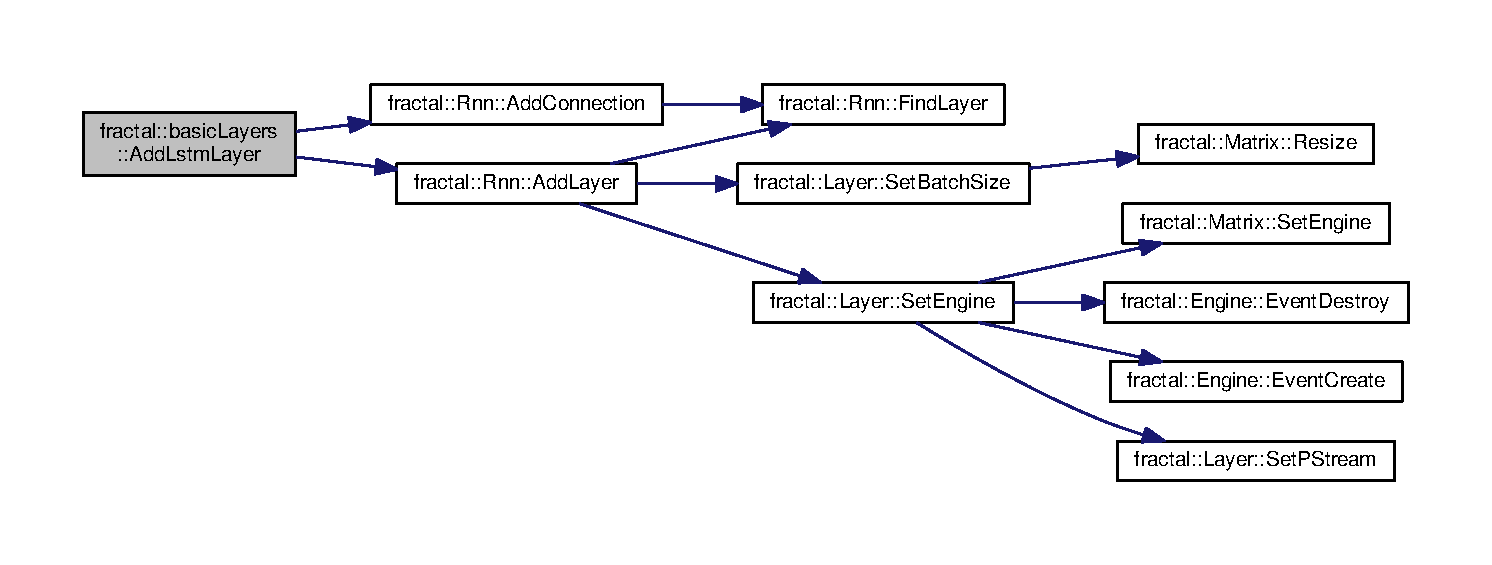
\includegraphics[width=350pt]{d9/d1c/namespacefractal_1_1basicLayers_a5b99ed6a0ad103b5fbff76a2d5c60480_cgraph}
\end{center}
\end{figure}



\hypertarget{namespacefractal_1_1cudaKernels}{\section{fractal\+:\+:cuda\+Kernels Namespace Reference}
\label{namespacefractal_1_1cudaKernels}\index{fractal\+::cuda\+Kernels@{fractal\+::cuda\+Kernels}}
}
\subsection*{Functions}
\begin{DoxyCompactItemize}
\item 
{\footnotesize template$<$class T $>$ }\\void \hyperlink{namespacefractal_1_1cudaKernels_a2f4f2776037a4f202000996e3da29b29}{Mem\+Set} (T $\ast$\+\_\+x, const T val, const unsigned long n, const cuda\+Stream\+\_\+t stream)
\item 
{\footnotesize template$<$class T $>$ }\\void \hyperlink{namespacefractal_1_1cudaKernels_af411d22b137514fd35f5da081eca1299}{Elem\+Mult} (const T $\ast$\+\_\+x, const T $\ast$\+\_\+y, T $\ast$\+\_\+z, const unsigned long n, const cuda\+Stream\+\_\+t stream)
\item 
{\footnotesize template$<$class T $>$ }\\void \hyperlink{namespacefractal_1_1cudaKernels_ad08024d3280d81d84bd682a608f1c70d}{Add} (const T $\ast$\+\_\+x, const T $\ast$\+\_\+y, T $\ast$\+\_\+z, const unsigned long n, const cuda\+Stream\+\_\+t stream)
\item 
{\footnotesize template$<$class T $>$ }\\void \hyperlink{namespacefractal_1_1cudaKernels_a0253e39cf1f3905c6aaa5f8fc875206a}{Func\+Sigmoid} (const T $\ast$\+\_\+x, T $\ast$\+\_\+y, const unsigned long n, const cuda\+Stream\+\_\+t stream)
\item 
{\footnotesize template$<$class T $>$ }\\void \hyperlink{namespacefractal_1_1cudaKernels_aab7275ddaf88bbdc0a340e1f6d1010a5}{Func\+Tanh} (const T $\ast$\+\_\+x, T $\ast$\+\_\+y, const unsigned long n, const cuda\+Stream\+\_\+t stream)
\item 
{\footnotesize template$<$class T $>$ }\\void \hyperlink{namespacefractal_1_1cudaKernels_a302c1507d587dd97bb1b0c0b4e5e6378}{Func\+Softplus} (const T $\ast$\+\_\+x, T $\ast$\+\_\+y, const unsigned long n, const cuda\+Stream\+\_\+t stream)
\item 
{\footnotesize template$<$class T $>$ }\\void \hyperlink{namespacefractal_1_1cudaKernels_a1214ead9e6a1af20689767f797e21ad7}{Func\+Rect\+Linear} (const T $\ast$\+\_\+x, T $\ast$\+\_\+y, const unsigned long n, const cuda\+Stream\+\_\+t stream)
\item 
{\footnotesize template$<$class T $>$ }\\void \hyperlink{namespacefractal_1_1cudaKernels_a715361cdca467605d0e1f1c617b3ab24}{Func\+Softmax} (const T $\ast$\+\_\+x, T $\ast$\+\_\+y, const unsigned long layer\+Size, const unsigned long batch\+Size, const cuda\+Stream\+\_\+t stream)
\item 
{\footnotesize template$<$class T $>$ }\\void \hyperlink{namespacefractal_1_1cudaKernels_a6feb31a8214d6d93c06164645f3f67ae}{Func\+Bound\+Range} (const T $\ast$\+\_\+x, T $\ast$\+\_\+y, const T min, const T max, const unsigned long n, const cuda\+Stream\+\_\+t stream)
\item 
{\footnotesize template$<$class T $>$ }\\void \hyperlink{namespacefractal_1_1cudaKernels_a694c2d619f8a1707e7ed0c74e9e5e952}{Func\+Sigmoid\+Deriv} (const T $\ast$\+\_\+x, T $\ast$\+\_\+y, const unsigned long n, const cuda\+Stream\+\_\+t stream)
\item 
{\footnotesize template$<$class T $>$ }\\void \hyperlink{namespacefractal_1_1cudaKernels_a68955cd20f3f388efca2144a0ed07925}{Func\+Tanh\+Deriv} (const T $\ast$\+\_\+x, T $\ast$\+\_\+y, const unsigned long n, const cuda\+Stream\+\_\+t stream)
\item 
{\footnotesize template$<$class T $>$ }\\void \hyperlink{namespacefractal_1_1cudaKernels_aba4be7ae2ab58b610d51df2fa9e7af73}{Func\+Softplus\+Deriv} (const T $\ast$\+\_\+x, T $\ast$\+\_\+y, const unsigned long n, const cuda\+Stream\+\_\+t stream)
\item 
{\footnotesize template$<$class T $>$ }\\void \hyperlink{namespacefractal_1_1cudaKernels_ae718cea5137940efd2fc610705cb06b2}{Func\+Rect\+Linear\+Deriv} (const T $\ast$\+\_\+x, T $\ast$\+\_\+y, const unsigned long n, const cuda\+Stream\+\_\+t stream)
\item 
{\footnotesize template$<$class T $>$ }\\void \hyperlink{namespacefractal_1_1cudaKernels_a596801702086d94d5078d612296a2207}{Rmsprop} (T $\ast$\+\_\+new\+Derivs, const T $\ast$\+\_\+derivs, T $\ast$\+\_\+ms\+Deriv, const T decay\+Rate, const unsigned long n, const cuda\+Stream\+\_\+t stream)
\item 
{\footnotesize template$<$class T $>$ }\\void \hyperlink{namespacefractal_1_1cudaKernels_a6ae4a4a96a55184eca0a59025292b6eb}{Adadelta} (T $\ast$\+\_\+deltas, const T $\ast$\+\_\+derivs, T $\ast$\+\_\+ms\+Deriv, T $\ast$\+\_\+ms\+Delta, const T learning\+Rate, const T decay\+Rate, const unsigned long n, const cuda\+Stream\+\_\+t stream)
\end{DoxyCompactItemize}


\subsection{Function Documentation}
\hypertarget{namespacefractal_1_1cudaKernels_a6ae4a4a96a55184eca0a59025292b6eb}{\index{fractal\+::cuda\+Kernels@{fractal\+::cuda\+Kernels}!Adadelta@{Adadelta}}
\index{Adadelta@{Adadelta}!fractal\+::cuda\+Kernels@{fractal\+::cuda\+Kernels}}
\subsubsection[{Adadelta}]{\setlength{\rightskip}{0pt plus 5cm}template$<$class T $>$ void fractal\+::cuda\+Kernels\+::\+Adadelta (
\begin{DoxyParamCaption}
\item[{T $\ast$}]{\+\_\+deltas, }
\item[{const T $\ast$}]{\+\_\+derivs, }
\item[{T $\ast$}]{\+\_\+ms\+Deriv, }
\item[{T $\ast$}]{\+\_\+ms\+Delta, }
\item[{const T}]{learning\+Rate, }
\item[{const T}]{decay\+Rate, }
\item[{const unsigned long}]{n, }
\item[{const cuda\+Stream\+\_\+t}]{stream}
\end{DoxyParamCaption}
)}}\label{namespacefractal_1_1cudaKernels_a6ae4a4a96a55184eca0a59025292b6eb}
\hypertarget{namespacefractal_1_1cudaKernels_ad08024d3280d81d84bd682a608f1c70d}{\index{fractal\+::cuda\+Kernels@{fractal\+::cuda\+Kernels}!Add@{Add}}
\index{Add@{Add}!fractal\+::cuda\+Kernels@{fractal\+::cuda\+Kernels}}
\subsubsection[{Add}]{\setlength{\rightskip}{0pt plus 5cm}template$<$class T $>$ void fractal\+::cuda\+Kernels\+::\+Add (
\begin{DoxyParamCaption}
\item[{const T $\ast$}]{\+\_\+x, }
\item[{const T $\ast$}]{\+\_\+y, }
\item[{T $\ast$}]{\+\_\+z, }
\item[{const unsigned long}]{n, }
\item[{const cuda\+Stream\+\_\+t}]{stream}
\end{DoxyParamCaption}
)}}\label{namespacefractal_1_1cudaKernels_ad08024d3280d81d84bd682a608f1c70d}
\hypertarget{namespacefractal_1_1cudaKernels_af411d22b137514fd35f5da081eca1299}{\index{fractal\+::cuda\+Kernels@{fractal\+::cuda\+Kernels}!Elem\+Mult@{Elem\+Mult}}
\index{Elem\+Mult@{Elem\+Mult}!fractal\+::cuda\+Kernels@{fractal\+::cuda\+Kernels}}
\subsubsection[{Elem\+Mult}]{\setlength{\rightskip}{0pt plus 5cm}template$<$class T $>$ void fractal\+::cuda\+Kernels\+::\+Elem\+Mult (
\begin{DoxyParamCaption}
\item[{const T $\ast$}]{\+\_\+x, }
\item[{const T $\ast$}]{\+\_\+y, }
\item[{T $\ast$}]{\+\_\+z, }
\item[{const unsigned long}]{n, }
\item[{const cuda\+Stream\+\_\+t}]{stream}
\end{DoxyParamCaption}
)}}\label{namespacefractal_1_1cudaKernels_af411d22b137514fd35f5da081eca1299}
\hypertarget{namespacefractal_1_1cudaKernels_a6feb31a8214d6d93c06164645f3f67ae}{\index{fractal\+::cuda\+Kernels@{fractal\+::cuda\+Kernels}!Func\+Bound\+Range@{Func\+Bound\+Range}}
\index{Func\+Bound\+Range@{Func\+Bound\+Range}!fractal\+::cuda\+Kernels@{fractal\+::cuda\+Kernels}}
\subsubsection[{Func\+Bound\+Range}]{\setlength{\rightskip}{0pt plus 5cm}template$<$class T $>$ void fractal\+::cuda\+Kernels\+::\+Func\+Bound\+Range (
\begin{DoxyParamCaption}
\item[{const T $\ast$}]{\+\_\+x, }
\item[{T $\ast$}]{\+\_\+y, }
\item[{const T}]{min, }
\item[{const T}]{max, }
\item[{const unsigned long}]{n, }
\item[{const cuda\+Stream\+\_\+t}]{stream}
\end{DoxyParamCaption}
)}}\label{namespacefractal_1_1cudaKernels_a6feb31a8214d6d93c06164645f3f67ae}


Here is the caller graph for this function\+:\nopagebreak
\begin{figure}[H]
\begin{center}
\leavevmode
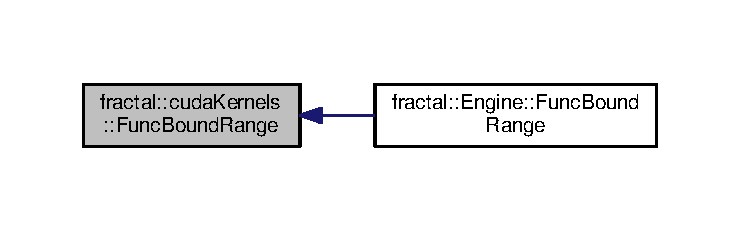
\includegraphics[width=350pt]{d3/d5d/namespacefractal_1_1cudaKernels_a6feb31a8214d6d93c06164645f3f67ae_icgraph}
\end{center}
\end{figure}


\hypertarget{namespacefractal_1_1cudaKernels_a1214ead9e6a1af20689767f797e21ad7}{\index{fractal\+::cuda\+Kernels@{fractal\+::cuda\+Kernels}!Func\+Rect\+Linear@{Func\+Rect\+Linear}}
\index{Func\+Rect\+Linear@{Func\+Rect\+Linear}!fractal\+::cuda\+Kernels@{fractal\+::cuda\+Kernels}}
\subsubsection[{Func\+Rect\+Linear}]{\setlength{\rightskip}{0pt plus 5cm}template$<$class T $>$ void fractal\+::cuda\+Kernels\+::\+Func\+Rect\+Linear (
\begin{DoxyParamCaption}
\item[{const T $\ast$}]{\+\_\+x, }
\item[{T $\ast$}]{\+\_\+y, }
\item[{const unsigned long}]{n, }
\item[{const cuda\+Stream\+\_\+t}]{stream}
\end{DoxyParamCaption}
)}}\label{namespacefractal_1_1cudaKernels_a1214ead9e6a1af20689767f797e21ad7}


Here is the caller graph for this function\+:\nopagebreak
\begin{figure}[H]
\begin{center}
\leavevmode
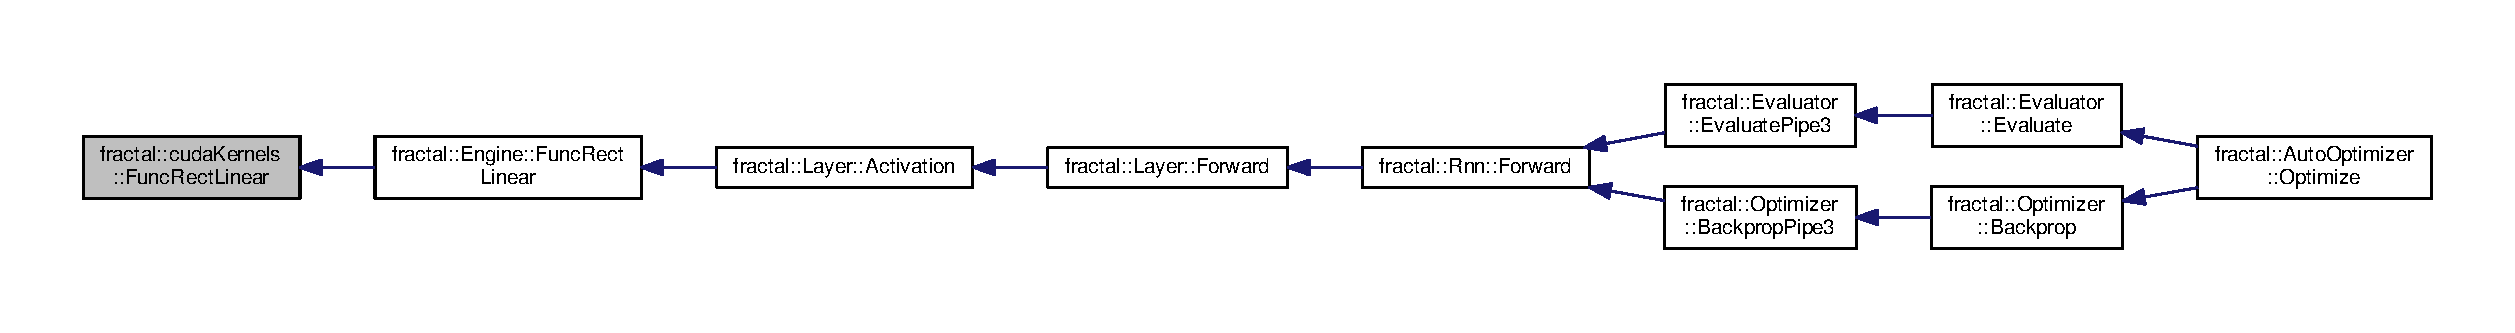
\includegraphics[width=350pt]{d3/d5d/namespacefractal_1_1cudaKernels_a1214ead9e6a1af20689767f797e21ad7_icgraph}
\end{center}
\end{figure}


\hypertarget{namespacefractal_1_1cudaKernels_ae718cea5137940efd2fc610705cb06b2}{\index{fractal\+::cuda\+Kernels@{fractal\+::cuda\+Kernels}!Func\+Rect\+Linear\+Deriv@{Func\+Rect\+Linear\+Deriv}}
\index{Func\+Rect\+Linear\+Deriv@{Func\+Rect\+Linear\+Deriv}!fractal\+::cuda\+Kernels@{fractal\+::cuda\+Kernels}}
\subsubsection[{Func\+Rect\+Linear\+Deriv}]{\setlength{\rightskip}{0pt plus 5cm}template$<$class T $>$ void fractal\+::cuda\+Kernels\+::\+Func\+Rect\+Linear\+Deriv (
\begin{DoxyParamCaption}
\item[{const T $\ast$}]{\+\_\+x, }
\item[{T $\ast$}]{\+\_\+y, }
\item[{const unsigned long}]{n, }
\item[{const cuda\+Stream\+\_\+t}]{stream}
\end{DoxyParamCaption}
)}}\label{namespacefractal_1_1cudaKernels_ae718cea5137940efd2fc610705cb06b2}
\hypertarget{namespacefractal_1_1cudaKernels_a0253e39cf1f3905c6aaa5f8fc875206a}{\index{fractal\+::cuda\+Kernels@{fractal\+::cuda\+Kernels}!Func\+Sigmoid@{Func\+Sigmoid}}
\index{Func\+Sigmoid@{Func\+Sigmoid}!fractal\+::cuda\+Kernels@{fractal\+::cuda\+Kernels}}
\subsubsection[{Func\+Sigmoid}]{\setlength{\rightskip}{0pt plus 5cm}template$<$class T $>$ void fractal\+::cuda\+Kernels\+::\+Func\+Sigmoid (
\begin{DoxyParamCaption}
\item[{const T $\ast$}]{\+\_\+x, }
\item[{T $\ast$}]{\+\_\+y, }
\item[{const unsigned long}]{n, }
\item[{const cuda\+Stream\+\_\+t}]{stream}
\end{DoxyParamCaption}
)}}\label{namespacefractal_1_1cudaKernels_a0253e39cf1f3905c6aaa5f8fc875206a}


Here is the caller graph for this function\+:\nopagebreak
\begin{figure}[H]
\begin{center}
\leavevmode
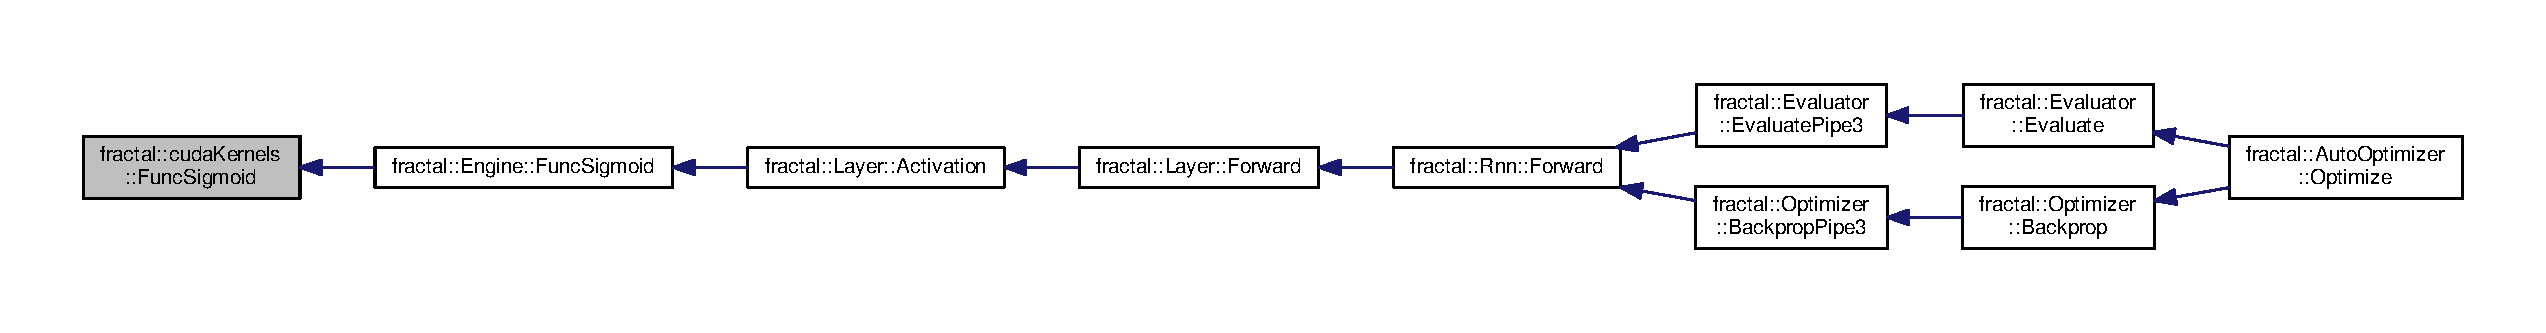
\includegraphics[width=350pt]{d3/d5d/namespacefractal_1_1cudaKernels_a0253e39cf1f3905c6aaa5f8fc875206a_icgraph}
\end{center}
\end{figure}


\hypertarget{namespacefractal_1_1cudaKernels_a694c2d619f8a1707e7ed0c74e9e5e952}{\index{fractal\+::cuda\+Kernels@{fractal\+::cuda\+Kernels}!Func\+Sigmoid\+Deriv@{Func\+Sigmoid\+Deriv}}
\index{Func\+Sigmoid\+Deriv@{Func\+Sigmoid\+Deriv}!fractal\+::cuda\+Kernels@{fractal\+::cuda\+Kernels}}
\subsubsection[{Func\+Sigmoid\+Deriv}]{\setlength{\rightskip}{0pt plus 5cm}template$<$class T $>$ void fractal\+::cuda\+Kernels\+::\+Func\+Sigmoid\+Deriv (
\begin{DoxyParamCaption}
\item[{const T $\ast$}]{\+\_\+x, }
\item[{T $\ast$}]{\+\_\+y, }
\item[{const unsigned long}]{n, }
\item[{const cuda\+Stream\+\_\+t}]{stream}
\end{DoxyParamCaption}
)}}\label{namespacefractal_1_1cudaKernels_a694c2d619f8a1707e7ed0c74e9e5e952}
\hypertarget{namespacefractal_1_1cudaKernels_a715361cdca467605d0e1f1c617b3ab24}{\index{fractal\+::cuda\+Kernels@{fractal\+::cuda\+Kernels}!Func\+Softmax@{Func\+Softmax}}
\index{Func\+Softmax@{Func\+Softmax}!fractal\+::cuda\+Kernels@{fractal\+::cuda\+Kernels}}
\subsubsection[{Func\+Softmax}]{\setlength{\rightskip}{0pt plus 5cm}template$<$class T $>$ void fractal\+::cuda\+Kernels\+::\+Func\+Softmax (
\begin{DoxyParamCaption}
\item[{const T $\ast$}]{\+\_\+x, }
\item[{T $\ast$}]{\+\_\+y, }
\item[{const unsigned long}]{layer\+Size, }
\item[{const unsigned long}]{batch\+Size, }
\item[{const cuda\+Stream\+\_\+t}]{stream}
\end{DoxyParamCaption}
)}}\label{namespacefractal_1_1cudaKernels_a715361cdca467605d0e1f1c617b3ab24}
\hypertarget{namespacefractal_1_1cudaKernels_a302c1507d587dd97bb1b0c0b4e5e6378}{\index{fractal\+::cuda\+Kernels@{fractal\+::cuda\+Kernels}!Func\+Softplus@{Func\+Softplus}}
\index{Func\+Softplus@{Func\+Softplus}!fractal\+::cuda\+Kernels@{fractal\+::cuda\+Kernels}}
\subsubsection[{Func\+Softplus}]{\setlength{\rightskip}{0pt plus 5cm}template$<$class T $>$ void fractal\+::cuda\+Kernels\+::\+Func\+Softplus (
\begin{DoxyParamCaption}
\item[{const T $\ast$}]{\+\_\+x, }
\item[{T $\ast$}]{\+\_\+y, }
\item[{const unsigned long}]{n, }
\item[{const cuda\+Stream\+\_\+t}]{stream}
\end{DoxyParamCaption}
)}}\label{namespacefractal_1_1cudaKernels_a302c1507d587dd97bb1b0c0b4e5e6378}


Here is the caller graph for this function\+:\nopagebreak
\begin{figure}[H]
\begin{center}
\leavevmode
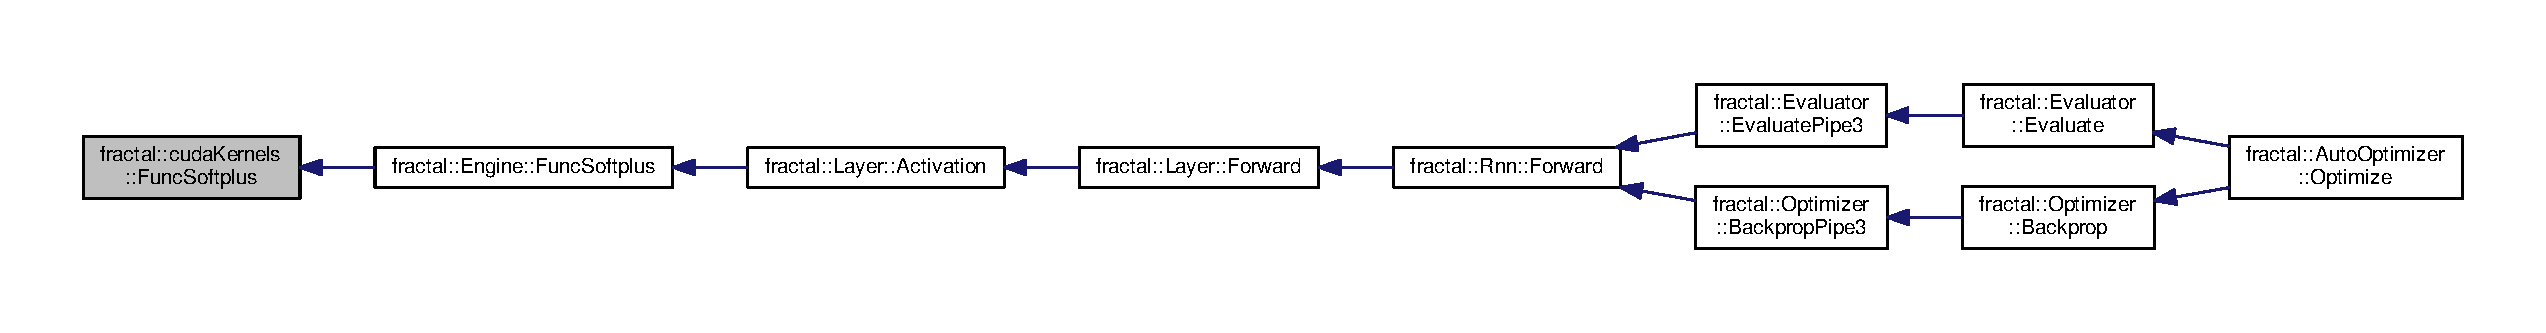
\includegraphics[width=350pt]{d3/d5d/namespacefractal_1_1cudaKernels_a302c1507d587dd97bb1b0c0b4e5e6378_icgraph}
\end{center}
\end{figure}


\hypertarget{namespacefractal_1_1cudaKernels_aba4be7ae2ab58b610d51df2fa9e7af73}{\index{fractal\+::cuda\+Kernels@{fractal\+::cuda\+Kernels}!Func\+Softplus\+Deriv@{Func\+Softplus\+Deriv}}
\index{Func\+Softplus\+Deriv@{Func\+Softplus\+Deriv}!fractal\+::cuda\+Kernels@{fractal\+::cuda\+Kernels}}
\subsubsection[{Func\+Softplus\+Deriv}]{\setlength{\rightskip}{0pt plus 5cm}template$<$class T $>$ void fractal\+::cuda\+Kernels\+::\+Func\+Softplus\+Deriv (
\begin{DoxyParamCaption}
\item[{const T $\ast$}]{\+\_\+x, }
\item[{T $\ast$}]{\+\_\+y, }
\item[{const unsigned long}]{n, }
\item[{const cuda\+Stream\+\_\+t}]{stream}
\end{DoxyParamCaption}
)}}\label{namespacefractal_1_1cudaKernels_aba4be7ae2ab58b610d51df2fa9e7af73}
\hypertarget{namespacefractal_1_1cudaKernels_aab7275ddaf88bbdc0a340e1f6d1010a5}{\index{fractal\+::cuda\+Kernels@{fractal\+::cuda\+Kernels}!Func\+Tanh@{Func\+Tanh}}
\index{Func\+Tanh@{Func\+Tanh}!fractal\+::cuda\+Kernels@{fractal\+::cuda\+Kernels}}
\subsubsection[{Func\+Tanh}]{\setlength{\rightskip}{0pt plus 5cm}template$<$class T $>$ void fractal\+::cuda\+Kernels\+::\+Func\+Tanh (
\begin{DoxyParamCaption}
\item[{const T $\ast$}]{\+\_\+x, }
\item[{T $\ast$}]{\+\_\+y, }
\item[{const unsigned long}]{n, }
\item[{const cuda\+Stream\+\_\+t}]{stream}
\end{DoxyParamCaption}
)}}\label{namespacefractal_1_1cudaKernels_aab7275ddaf88bbdc0a340e1f6d1010a5}


Here is the caller graph for this function\+:\nopagebreak
\begin{figure}[H]
\begin{center}
\leavevmode
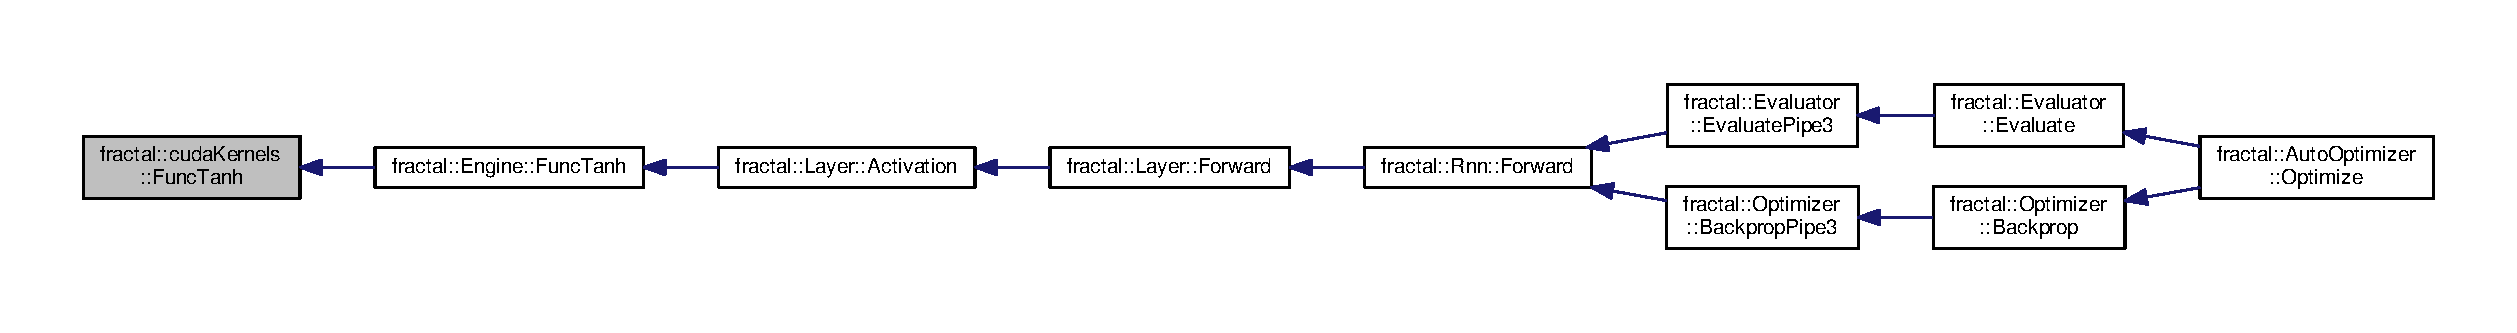
\includegraphics[width=350pt]{d3/d5d/namespacefractal_1_1cudaKernels_aab7275ddaf88bbdc0a340e1f6d1010a5_icgraph}
\end{center}
\end{figure}


\hypertarget{namespacefractal_1_1cudaKernels_a68955cd20f3f388efca2144a0ed07925}{\index{fractal\+::cuda\+Kernels@{fractal\+::cuda\+Kernels}!Func\+Tanh\+Deriv@{Func\+Tanh\+Deriv}}
\index{Func\+Tanh\+Deriv@{Func\+Tanh\+Deriv}!fractal\+::cuda\+Kernels@{fractal\+::cuda\+Kernels}}
\subsubsection[{Func\+Tanh\+Deriv}]{\setlength{\rightskip}{0pt plus 5cm}template$<$class T $>$ void fractal\+::cuda\+Kernels\+::\+Func\+Tanh\+Deriv (
\begin{DoxyParamCaption}
\item[{const T $\ast$}]{\+\_\+x, }
\item[{T $\ast$}]{\+\_\+y, }
\item[{const unsigned long}]{n, }
\item[{const cuda\+Stream\+\_\+t}]{stream}
\end{DoxyParamCaption}
)}}\label{namespacefractal_1_1cudaKernels_a68955cd20f3f388efca2144a0ed07925}
\hypertarget{namespacefractal_1_1cudaKernels_a2f4f2776037a4f202000996e3da29b29}{\index{fractal\+::cuda\+Kernels@{fractal\+::cuda\+Kernels}!Mem\+Set@{Mem\+Set}}
\index{Mem\+Set@{Mem\+Set}!fractal\+::cuda\+Kernels@{fractal\+::cuda\+Kernels}}
\subsubsection[{Mem\+Set}]{\setlength{\rightskip}{0pt plus 5cm}template$<$class T $>$ void fractal\+::cuda\+Kernels\+::\+Mem\+Set (
\begin{DoxyParamCaption}
\item[{T $\ast$}]{\+\_\+x, }
\item[{const T}]{val, }
\item[{const unsigned long}]{n, }
\item[{const cuda\+Stream\+\_\+t}]{stream}
\end{DoxyParamCaption}
)}}\label{namespacefractal_1_1cudaKernels_a2f4f2776037a4f202000996e3da29b29}
\hypertarget{namespacefractal_1_1cudaKernels_a596801702086d94d5078d612296a2207}{\index{fractal\+::cuda\+Kernels@{fractal\+::cuda\+Kernels}!Rmsprop@{Rmsprop}}
\index{Rmsprop@{Rmsprop}!fractal\+::cuda\+Kernels@{fractal\+::cuda\+Kernels}}
\subsubsection[{Rmsprop}]{\setlength{\rightskip}{0pt plus 5cm}template$<$class T $>$ void fractal\+::cuda\+Kernels\+::\+Rmsprop (
\begin{DoxyParamCaption}
\item[{T $\ast$}]{\+\_\+new\+Derivs, }
\item[{const T $\ast$}]{\+\_\+derivs, }
\item[{T $\ast$}]{\+\_\+ms\+Deriv, }
\item[{const T}]{decay\+Rate, }
\item[{const unsigned long}]{n, }
\item[{const cuda\+Stream\+\_\+t}]{stream}
\end{DoxyParamCaption}
)}}\label{namespacefractal_1_1cudaKernels_a596801702086d94d5078d612296a2207}

\chapter{Class Documentation}
\hypertarget{classfractal_1_1AutoOptimizer}{\section{fractal\+:\+:Auto\+Optimizer Class Reference}
\label{classfractal_1_1AutoOptimizer}\index{fractal\+::\+Auto\+Optimizer@{fractal\+::\+Auto\+Optimizer}}
}


{\ttfamily \#include $<$Auto\+Optimizer.\+h$>$}

\subsection*{Public Member Functions}
\begin{DoxyCompactItemize}
\item 
\hyperlink{classfractal_1_1AutoOptimizer_a256411fbacb9251bd378d64e6cbf01d3}{Auto\+Optimizer} ()
\item 
virtual \hyperlink{classfractal_1_1AutoOptimizer_acc67d4d6dcd986151cda294e9a937235}{$\sim$\+Auto\+Optimizer} ()
\item 
void \hyperlink{classfractal_1_1AutoOptimizer_afd0ac1c7fc8ee5ac80fabd38fa8891c7}{Optimize} (\hyperlink{classfractal_1_1Rnn}{Rnn} \&rnn, \hyperlink{classfractal_1_1Stream}{Stream} \&train\+Stream, \hyperlink{classfractal_1_1Stream}{Stream} \&eval\+Stream, \hyperlink{classfractal_1_1Evaluator}{Evaluator} \&evaluator, const \hyperlink{namespacefractal_a9697dee0746adccf37331470de749c2b}{Port\+Map\+List} \&input\+Ports, const \hyperlink{namespacefractal_a9697dee0746adccf37331470de749c2b}{Port\+Map\+List} \&output\+Ports, const unsigned long n\+Train\+Frame\+Per\+Epoch, const unsigned long n\+Eval\+Frame\+Per\+Epoch, const unsigned long window\+Size, const unsigned long step\+Size)
\item 
void \hyperlink{classfractal_1_1AutoOptimizer_ab54934b953c1b8fe43daf8ae842c1e72}{Set\+Workspace\+Path} (const std\+::string \&path)
\item 
void \hyperlink{classfractal_1_1AutoOptimizer_aa89945094acb81bc70df7811fb2b8e4b}{Set\+Init\+Learning\+Rate} (const \hyperlink{namespacefractal_a1c2d2530689575d5ccb56bae52af70d3}{F\+L\+O\+A\+T} val)
\item 
void \hyperlink{classfractal_1_1AutoOptimizer_a2bcb64164719207cc07363ed691bdbdf}{Set\+Min\+Learning\+Rate} (const \hyperlink{namespacefractal_a1c2d2530689575d5ccb56bae52af70d3}{F\+L\+O\+A\+T} val)
\item 
void \hyperlink{classfractal_1_1AutoOptimizer_a180cb033daeb09a77e310e6f8db390ee}{Set\+Momentum} (const \hyperlink{namespacefractal_a1c2d2530689575d5ccb56bae52af70d3}{F\+L\+O\+A\+T} val)
\item 
void \hyperlink{classfractal_1_1AutoOptimizer_a952cb29558d31e51b5dd660a3feabea4}{Set\+Rmsprop} (const bool val)
\item 
void \hyperlink{classfractal_1_1AutoOptimizer_aa89f019725afed0d82ed44580ad67041}{Set\+Adadelta} (const bool val)
\item 
void \hyperlink{classfractal_1_1AutoOptimizer_a77cc8ed1ad995342a795dd0bfcfdbca9}{Set\+Rms\+Decay\+Rate} (const \hyperlink{namespacefractal_a1c2d2530689575d5ccb56bae52af70d3}{F\+L\+O\+A\+T} val)
\item 
void \hyperlink{classfractal_1_1AutoOptimizer_a952ed95e33579334a22ebad63cd5a3a1}{Set\+Max\+Retry\+Count} (const unsigned long val)
\item 
void \hyperlink{classfractal_1_1AutoOptimizer_a34def384fd138ba5b986ceac988d7cd2}{Set\+Learning\+Rate\+Decay\+Rate} (const \hyperlink{namespacefractal_a1c2d2530689575d5ccb56bae52af70d3}{F\+L\+O\+A\+T} val)
\item 
void \hyperlink{classfractal_1_1AutoOptimizer_ad8ff2b8b03172470c3f6e04e6c80e2e5}{Set\+Lambda\+Loss} (std\+::function$<$ double(\hyperlink{classfractal_1_1Evaluator}{Evaluator} \&)$>$ lambda)
\item 
void \hyperlink{classfractal_1_1AutoOptimizer_a599d01238939f6e6b7edc17a2c75837f}{Set\+Lambda\+Post\+Eval} (std\+::function$<$ void(\hyperlink{classfractal_1_1Evaluator}{Evaluator} \&)$>$ lambda)
\item 
const std\+::string \& \hyperlink{classfractal_1_1AutoOptimizer_a40ddbe471d220a99ff63b5f6e36d9f23}{Get\+Workspace\+Path} ()
\item 
const \hyperlink{namespacefractal_a1c2d2530689575d5ccb56bae52af70d3}{F\+L\+O\+A\+T} \hyperlink{classfractal_1_1AutoOptimizer_a615800e1d9f8a74e059c6cefd8ae34a7}{Get\+Init\+Learning\+Rate} ()
\item 
const \hyperlink{namespacefractal_a1c2d2530689575d5ccb56bae52af70d3}{F\+L\+O\+A\+T} \hyperlink{classfractal_1_1AutoOptimizer_a62c50420cc7a21afccfe6dd1851cea08}{Get\+Min\+Learning\+Rate} ()
\item 
const \hyperlink{namespacefractal_a1c2d2530689575d5ccb56bae52af70d3}{F\+L\+O\+A\+T} \hyperlink{classfractal_1_1AutoOptimizer_afbabc25af9b3e25a9d574ecb4fb21d8b}{Get\+Momentum} ()
\item 
const bool \hyperlink{classfractal_1_1AutoOptimizer_a267e331f05ab03a7342c8b335894780f}{Get\+Rmsprop} ()
\item 
const bool \hyperlink{classfractal_1_1AutoOptimizer_a3ea55a1c6bcefea20d73566c6daa274d}{Get\+Adadelta} ()
\item 
const \hyperlink{namespacefractal_a1c2d2530689575d5ccb56bae52af70d3}{F\+L\+O\+A\+T} \hyperlink{classfractal_1_1AutoOptimizer_af4698e9f1d10bb66983b228b6f420ff1}{Get\+Rms\+Decay\+Rate} ()
\item 
const unsigned long \hyperlink{classfractal_1_1AutoOptimizer_a54cd7b56cb4436b9a7cffc201d9b7c9b}{Get\+Max\+Retry\+Count} ()
\item 
const \hyperlink{namespacefractal_a1c2d2530689575d5ccb56bae52af70d3}{F\+L\+O\+A\+T} \hyperlink{classfractal_1_1AutoOptimizer_aaa5835c8a82b8b02ba5b81aa8af449c9}{Get\+Learning\+Rate\+Decay\+Rate} ()
\end{DoxyCompactItemize}
\subsection*{Protected Attributes}
\begin{DoxyCompactItemize}
\item 
std\+::function$<$ double(\hyperlink{classfractal_1_1Evaluator}{Evaluator} \&)$>$ \hyperlink{classfractal_1_1AutoOptimizer_a6e9db9d03a39a7f9c3754562d54c8e6b}{lambda\+Loss}
\item 
std\+::function$<$ void(\hyperlink{classfractal_1_1Evaluator}{Evaluator} \&)$>$ \hyperlink{classfractal_1_1AutoOptimizer_a0b32551c87870d815b3333315fc72a31}{lambda\+Post\+Eval}
\item 
std\+::string \hyperlink{classfractal_1_1AutoOptimizer_a2395471e6bc9585b3a42295a030a6f80}{workspace\+Path}
\item 
\hyperlink{namespacefractal_a1c2d2530689575d5ccb56bae52af70d3}{F\+L\+O\+A\+T} \hyperlink{classfractal_1_1AutoOptimizer_a45091ce24c1eff24e60644d2d5eddb0a}{init\+Learning\+Rate}
\item 
\hyperlink{namespacefractal_a1c2d2530689575d5ccb56bae52af70d3}{F\+L\+O\+A\+T} \hyperlink{classfractal_1_1AutoOptimizer_aefc6501717ce6fc3ad1ea83ee8743c01}{min\+Learning\+Rate}
\item 
\hyperlink{namespacefractal_a1c2d2530689575d5ccb56bae52af70d3}{F\+L\+O\+A\+T} \hyperlink{classfractal_1_1AutoOptimizer_a06a388ab208b871f47edd111aad33f78}{momentum}
\item 
bool \hyperlink{classfractal_1_1AutoOptimizer_a358367f581267c957fc7fe705b19ece2}{rmsprop}
\item 
bool \hyperlink{classfractal_1_1AutoOptimizer_a7b41188a4a23629e69144073493d317f}{adadelta}
\item 
\hyperlink{namespacefractal_a1c2d2530689575d5ccb56bae52af70d3}{F\+L\+O\+A\+T} \hyperlink{classfractal_1_1AutoOptimizer_a83f0519b89b1a33810fec7503a35f732}{rms\+Decay\+Rate}
\item 
\hyperlink{namespacefractal_a1c2d2530689575d5ccb56bae52af70d3}{F\+L\+O\+A\+T} \hyperlink{classfractal_1_1AutoOptimizer_a063181ceec0a4c7f4e98ba15b74ae6a8}{learning\+Rate\+Decay\+Rate}
\item 
unsigned long \hyperlink{classfractal_1_1AutoOptimizer_a2cf0c04067aba8fd08551d9a973d3de3}{max\+Retry\+Count}
\end{DoxyCompactItemize}


\subsection{Detailed Description}


Definition at line 32 of file Auto\+Optimizer.\+h.



\subsection{Constructor \& Destructor Documentation}
\hypertarget{classfractal_1_1AutoOptimizer_a256411fbacb9251bd378d64e6cbf01d3}{\index{fractal\+::\+Auto\+Optimizer@{fractal\+::\+Auto\+Optimizer}!Auto\+Optimizer@{Auto\+Optimizer}}
\index{Auto\+Optimizer@{Auto\+Optimizer}!fractal\+::\+Auto\+Optimizer@{fractal\+::\+Auto\+Optimizer}}
\subsubsection[{Auto\+Optimizer}]{\setlength{\rightskip}{0pt plus 5cm}fractal\+::\+Auto\+Optimizer\+::\+Auto\+Optimizer (
\begin{DoxyParamCaption}
{}
\end{DoxyParamCaption}
)}}\label{classfractal_1_1AutoOptimizer_a256411fbacb9251bd378d64e6cbf01d3}


Definition at line 28 of file Auto\+Optimizer.\+cc.

\hypertarget{classfractal_1_1AutoOptimizer_acc67d4d6dcd986151cda294e9a937235}{\index{fractal\+::\+Auto\+Optimizer@{fractal\+::\+Auto\+Optimizer}!````~Auto\+Optimizer@{$\sim$\+Auto\+Optimizer}}
\index{````~Auto\+Optimizer@{$\sim$\+Auto\+Optimizer}!fractal\+::\+Auto\+Optimizer@{fractal\+::\+Auto\+Optimizer}}
\subsubsection[{$\sim$\+Auto\+Optimizer}]{\setlength{\rightskip}{0pt plus 5cm}virtual fractal\+::\+Auto\+Optimizer\+::$\sim$\+Auto\+Optimizer (
\begin{DoxyParamCaption}
{}
\end{DoxyParamCaption}
)\hspace{0.3cm}{\ttfamily [inline]}, {\ttfamily [virtual]}}}\label{classfractal_1_1AutoOptimizer_acc67d4d6dcd986151cda294e9a937235}


Definition at line 36 of file Auto\+Optimizer.\+h.



\subsection{Member Function Documentation}
\hypertarget{classfractal_1_1AutoOptimizer_a3ea55a1c6bcefea20d73566c6daa274d}{\index{fractal\+::\+Auto\+Optimizer@{fractal\+::\+Auto\+Optimizer}!Get\+Adadelta@{Get\+Adadelta}}
\index{Get\+Adadelta@{Get\+Adadelta}!fractal\+::\+Auto\+Optimizer@{fractal\+::\+Auto\+Optimizer}}
\subsubsection[{Get\+Adadelta}]{\setlength{\rightskip}{0pt plus 5cm}const bool fractal\+::\+Auto\+Optimizer\+::\+Get\+Adadelta (
\begin{DoxyParamCaption}
{}
\end{DoxyParamCaption}
)\hspace{0.3cm}{\ttfamily [inline]}}}\label{classfractal_1_1AutoOptimizer_a3ea55a1c6bcefea20d73566c6daa274d}


Definition at line 61 of file Auto\+Optimizer.\+h.

\hypertarget{classfractal_1_1AutoOptimizer_a615800e1d9f8a74e059c6cefd8ae34a7}{\index{fractal\+::\+Auto\+Optimizer@{fractal\+::\+Auto\+Optimizer}!Get\+Init\+Learning\+Rate@{Get\+Init\+Learning\+Rate}}
\index{Get\+Init\+Learning\+Rate@{Get\+Init\+Learning\+Rate}!fractal\+::\+Auto\+Optimizer@{fractal\+::\+Auto\+Optimizer}}
\subsubsection[{Get\+Init\+Learning\+Rate}]{\setlength{\rightskip}{0pt plus 5cm}const {\bf F\+L\+O\+A\+T} fractal\+::\+Auto\+Optimizer\+::\+Get\+Init\+Learning\+Rate (
\begin{DoxyParamCaption}
{}
\end{DoxyParamCaption}
)\hspace{0.3cm}{\ttfamily [inline]}}}\label{classfractal_1_1AutoOptimizer_a615800e1d9f8a74e059c6cefd8ae34a7}


Definition at line 57 of file Auto\+Optimizer.\+h.

\hypertarget{classfractal_1_1AutoOptimizer_aaa5835c8a82b8b02ba5b81aa8af449c9}{\index{fractal\+::\+Auto\+Optimizer@{fractal\+::\+Auto\+Optimizer}!Get\+Learning\+Rate\+Decay\+Rate@{Get\+Learning\+Rate\+Decay\+Rate}}
\index{Get\+Learning\+Rate\+Decay\+Rate@{Get\+Learning\+Rate\+Decay\+Rate}!fractal\+::\+Auto\+Optimizer@{fractal\+::\+Auto\+Optimizer}}
\subsubsection[{Get\+Learning\+Rate\+Decay\+Rate}]{\setlength{\rightskip}{0pt plus 5cm}const {\bf F\+L\+O\+A\+T} fractal\+::\+Auto\+Optimizer\+::\+Get\+Learning\+Rate\+Decay\+Rate (
\begin{DoxyParamCaption}
{}
\end{DoxyParamCaption}
)\hspace{0.3cm}{\ttfamily [inline]}}}\label{classfractal_1_1AutoOptimizer_aaa5835c8a82b8b02ba5b81aa8af449c9}


Definition at line 64 of file Auto\+Optimizer.\+h.

\hypertarget{classfractal_1_1AutoOptimizer_a54cd7b56cb4436b9a7cffc201d9b7c9b}{\index{fractal\+::\+Auto\+Optimizer@{fractal\+::\+Auto\+Optimizer}!Get\+Max\+Retry\+Count@{Get\+Max\+Retry\+Count}}
\index{Get\+Max\+Retry\+Count@{Get\+Max\+Retry\+Count}!fractal\+::\+Auto\+Optimizer@{fractal\+::\+Auto\+Optimizer}}
\subsubsection[{Get\+Max\+Retry\+Count}]{\setlength{\rightskip}{0pt plus 5cm}const unsigned long fractal\+::\+Auto\+Optimizer\+::\+Get\+Max\+Retry\+Count (
\begin{DoxyParamCaption}
{}
\end{DoxyParamCaption}
)\hspace{0.3cm}{\ttfamily [inline]}}}\label{classfractal_1_1AutoOptimizer_a54cd7b56cb4436b9a7cffc201d9b7c9b}


Definition at line 63 of file Auto\+Optimizer.\+h.

\hypertarget{classfractal_1_1AutoOptimizer_a62c50420cc7a21afccfe6dd1851cea08}{\index{fractal\+::\+Auto\+Optimizer@{fractal\+::\+Auto\+Optimizer}!Get\+Min\+Learning\+Rate@{Get\+Min\+Learning\+Rate}}
\index{Get\+Min\+Learning\+Rate@{Get\+Min\+Learning\+Rate}!fractal\+::\+Auto\+Optimizer@{fractal\+::\+Auto\+Optimizer}}
\subsubsection[{Get\+Min\+Learning\+Rate}]{\setlength{\rightskip}{0pt plus 5cm}const {\bf F\+L\+O\+A\+T} fractal\+::\+Auto\+Optimizer\+::\+Get\+Min\+Learning\+Rate (
\begin{DoxyParamCaption}
{}
\end{DoxyParamCaption}
)\hspace{0.3cm}{\ttfamily [inline]}}}\label{classfractal_1_1AutoOptimizer_a62c50420cc7a21afccfe6dd1851cea08}


Definition at line 58 of file Auto\+Optimizer.\+h.

\hypertarget{classfractal_1_1AutoOptimizer_afbabc25af9b3e25a9d574ecb4fb21d8b}{\index{fractal\+::\+Auto\+Optimizer@{fractal\+::\+Auto\+Optimizer}!Get\+Momentum@{Get\+Momentum}}
\index{Get\+Momentum@{Get\+Momentum}!fractal\+::\+Auto\+Optimizer@{fractal\+::\+Auto\+Optimizer}}
\subsubsection[{Get\+Momentum}]{\setlength{\rightskip}{0pt plus 5cm}const {\bf F\+L\+O\+A\+T} fractal\+::\+Auto\+Optimizer\+::\+Get\+Momentum (
\begin{DoxyParamCaption}
{}
\end{DoxyParamCaption}
)\hspace{0.3cm}{\ttfamily [inline]}}}\label{classfractal_1_1AutoOptimizer_afbabc25af9b3e25a9d574ecb4fb21d8b}


Definition at line 59 of file Auto\+Optimizer.\+h.

\hypertarget{classfractal_1_1AutoOptimizer_af4698e9f1d10bb66983b228b6f420ff1}{\index{fractal\+::\+Auto\+Optimizer@{fractal\+::\+Auto\+Optimizer}!Get\+Rms\+Decay\+Rate@{Get\+Rms\+Decay\+Rate}}
\index{Get\+Rms\+Decay\+Rate@{Get\+Rms\+Decay\+Rate}!fractal\+::\+Auto\+Optimizer@{fractal\+::\+Auto\+Optimizer}}
\subsubsection[{Get\+Rms\+Decay\+Rate}]{\setlength{\rightskip}{0pt plus 5cm}const {\bf F\+L\+O\+A\+T} fractal\+::\+Auto\+Optimizer\+::\+Get\+Rms\+Decay\+Rate (
\begin{DoxyParamCaption}
{}
\end{DoxyParamCaption}
)\hspace{0.3cm}{\ttfamily [inline]}}}\label{classfractal_1_1AutoOptimizer_af4698e9f1d10bb66983b228b6f420ff1}


Definition at line 62 of file Auto\+Optimizer.\+h.

\hypertarget{classfractal_1_1AutoOptimizer_a267e331f05ab03a7342c8b335894780f}{\index{fractal\+::\+Auto\+Optimizer@{fractal\+::\+Auto\+Optimizer}!Get\+Rmsprop@{Get\+Rmsprop}}
\index{Get\+Rmsprop@{Get\+Rmsprop}!fractal\+::\+Auto\+Optimizer@{fractal\+::\+Auto\+Optimizer}}
\subsubsection[{Get\+Rmsprop}]{\setlength{\rightskip}{0pt plus 5cm}const bool fractal\+::\+Auto\+Optimizer\+::\+Get\+Rmsprop (
\begin{DoxyParamCaption}
{}
\end{DoxyParamCaption}
)\hspace{0.3cm}{\ttfamily [inline]}}}\label{classfractal_1_1AutoOptimizer_a267e331f05ab03a7342c8b335894780f}


Definition at line 60 of file Auto\+Optimizer.\+h.

\hypertarget{classfractal_1_1AutoOptimizer_a40ddbe471d220a99ff63b5f6e36d9f23}{\index{fractal\+::\+Auto\+Optimizer@{fractal\+::\+Auto\+Optimizer}!Get\+Workspace\+Path@{Get\+Workspace\+Path}}
\index{Get\+Workspace\+Path@{Get\+Workspace\+Path}!fractal\+::\+Auto\+Optimizer@{fractal\+::\+Auto\+Optimizer}}
\subsubsection[{Get\+Workspace\+Path}]{\setlength{\rightskip}{0pt plus 5cm}const std\+::string\& fractal\+::\+Auto\+Optimizer\+::\+Get\+Workspace\+Path (
\begin{DoxyParamCaption}
{}
\end{DoxyParamCaption}
)\hspace{0.3cm}{\ttfamily [inline]}}}\label{classfractal_1_1AutoOptimizer_a40ddbe471d220a99ff63b5f6e36d9f23}


Definition at line 56 of file Auto\+Optimizer.\+h.

\hypertarget{classfractal_1_1AutoOptimizer_afd0ac1c7fc8ee5ac80fabd38fa8891c7}{\index{fractal\+::\+Auto\+Optimizer@{fractal\+::\+Auto\+Optimizer}!Optimize@{Optimize}}
\index{Optimize@{Optimize}!fractal\+::\+Auto\+Optimizer@{fractal\+::\+Auto\+Optimizer}}
\subsubsection[{Optimize}]{\setlength{\rightskip}{0pt plus 5cm}void fractal\+::\+Auto\+Optimizer\+::\+Optimize (
\begin{DoxyParamCaption}
\item[{{\bf Rnn} \&}]{rnn, }
\item[{{\bf Stream} \&}]{train\+Stream, }
\item[{{\bf Stream} \&}]{eval\+Stream, }
\item[{{\bf Evaluator} \&}]{evaluator, }
\item[{const {\bf Port\+Map\+List} \&}]{input\+Ports, }
\item[{const {\bf Port\+Map\+List} \&}]{output\+Ports, }
\item[{const unsigned long}]{n\+Train\+Frame\+Per\+Epoch, }
\item[{const unsigned long}]{n\+Eval\+Frame\+Per\+Epoch, }
\item[{const unsigned long}]{window\+Size, }
\item[{const unsigned long}]{step\+Size}
\end{DoxyParamCaption}
)}}\label{classfractal_1_1AutoOptimizer_afd0ac1c7fc8ee5ac80fabd38fa8891c7}


Definition at line 65 of file Auto\+Optimizer.\+cc.



Here is the call graph for this function\+:\nopagebreak
\begin{figure}[H]
\begin{center}
\leavevmode
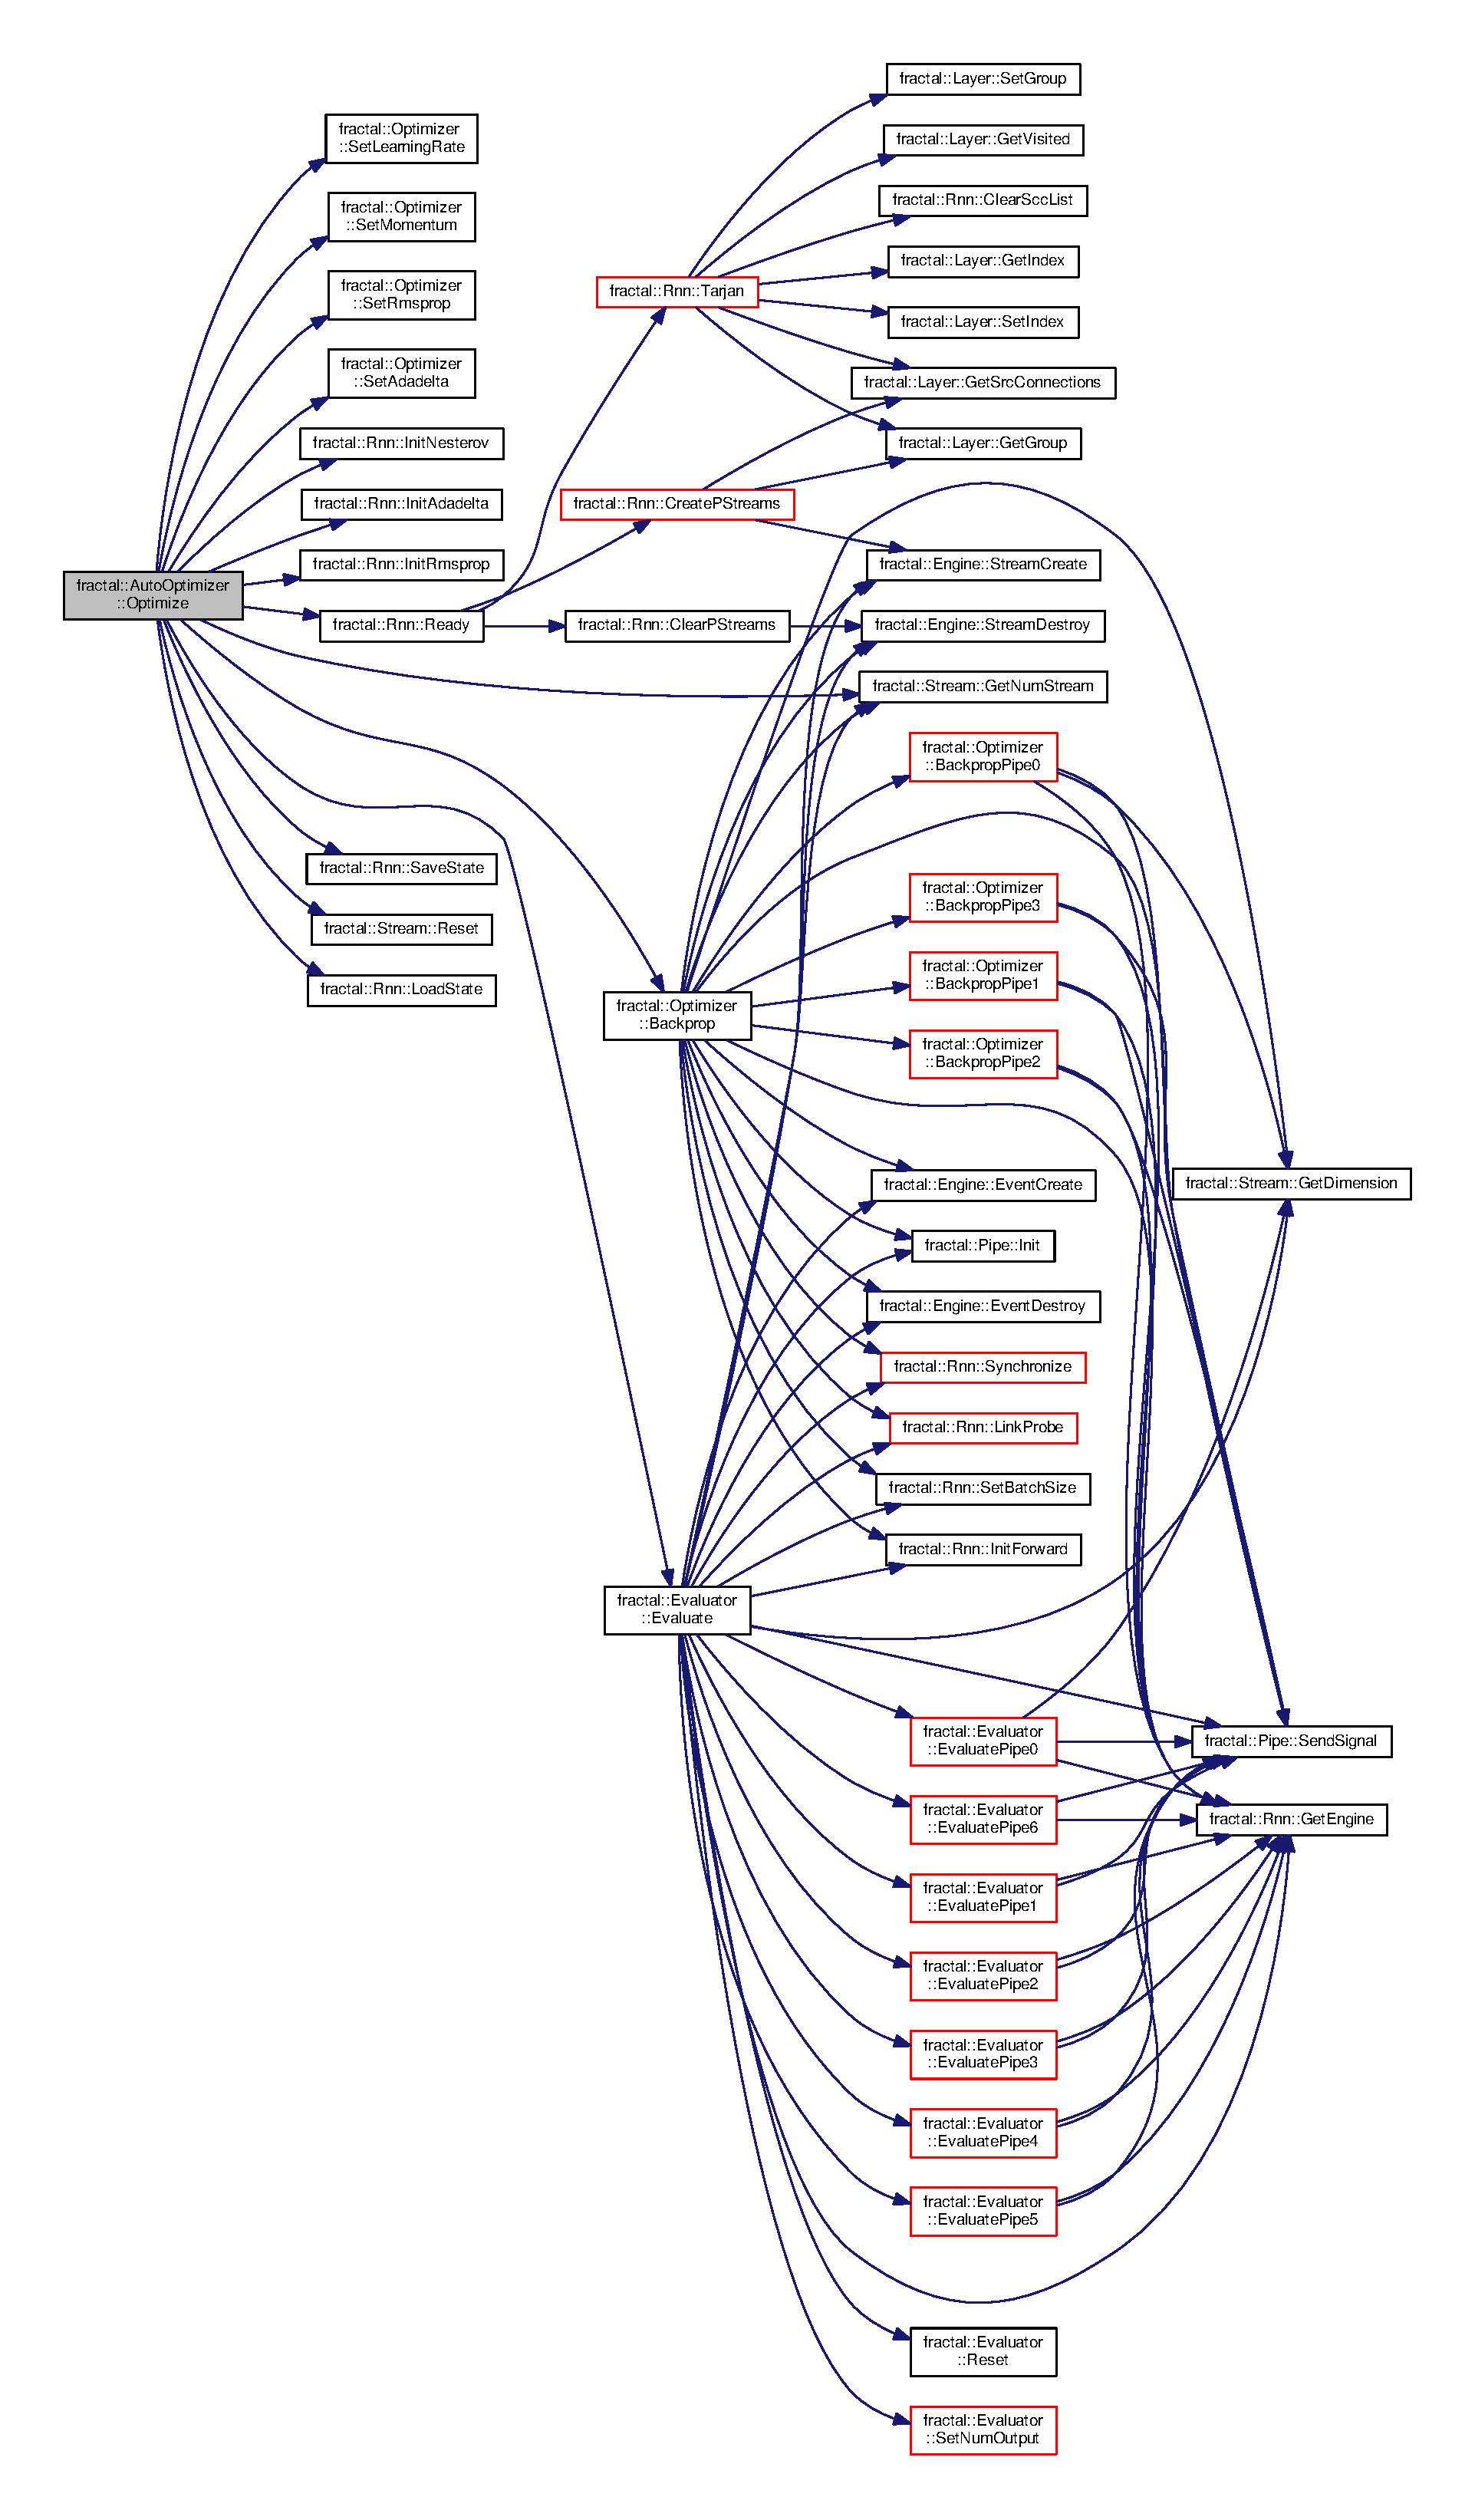
\includegraphics[height=550pt]{d0/dc0/classfractal_1_1AutoOptimizer_afd0ac1c7fc8ee5ac80fabd38fa8891c7_cgraph}
\end{center}
\end{figure}


\hypertarget{classfractal_1_1AutoOptimizer_aa89f019725afed0d82ed44580ad67041}{\index{fractal\+::\+Auto\+Optimizer@{fractal\+::\+Auto\+Optimizer}!Set\+Adadelta@{Set\+Adadelta}}
\index{Set\+Adadelta@{Set\+Adadelta}!fractal\+::\+Auto\+Optimizer@{fractal\+::\+Auto\+Optimizer}}
\subsubsection[{Set\+Adadelta}]{\setlength{\rightskip}{0pt plus 5cm}void fractal\+::\+Auto\+Optimizer\+::\+Set\+Adadelta (
\begin{DoxyParamCaption}
\item[{const bool}]{val}
\end{DoxyParamCaption}
)\hspace{0.3cm}{\ttfamily [inline]}}}\label{classfractal_1_1AutoOptimizer_aa89f019725afed0d82ed44580ad67041}


Definition at line 48 of file Auto\+Optimizer.\+h.

\hypertarget{classfractal_1_1AutoOptimizer_aa89945094acb81bc70df7811fb2b8e4b}{\index{fractal\+::\+Auto\+Optimizer@{fractal\+::\+Auto\+Optimizer}!Set\+Init\+Learning\+Rate@{Set\+Init\+Learning\+Rate}}
\index{Set\+Init\+Learning\+Rate@{Set\+Init\+Learning\+Rate}!fractal\+::\+Auto\+Optimizer@{fractal\+::\+Auto\+Optimizer}}
\subsubsection[{Set\+Init\+Learning\+Rate}]{\setlength{\rightskip}{0pt plus 5cm}void fractal\+::\+Auto\+Optimizer\+::\+Set\+Init\+Learning\+Rate (
\begin{DoxyParamCaption}
\item[{const {\bf F\+L\+O\+A\+T}}]{val}
\end{DoxyParamCaption}
)\hspace{0.3cm}{\ttfamily [inline]}}}\label{classfractal_1_1AutoOptimizer_aa89945094acb81bc70df7811fb2b8e4b}


Definition at line 44 of file Auto\+Optimizer.\+h.

\hypertarget{classfractal_1_1AutoOptimizer_ad8ff2b8b03172470c3f6e04e6c80e2e5}{\index{fractal\+::\+Auto\+Optimizer@{fractal\+::\+Auto\+Optimizer}!Set\+Lambda\+Loss@{Set\+Lambda\+Loss}}
\index{Set\+Lambda\+Loss@{Set\+Lambda\+Loss}!fractal\+::\+Auto\+Optimizer@{fractal\+::\+Auto\+Optimizer}}
\subsubsection[{Set\+Lambda\+Loss}]{\setlength{\rightskip}{0pt plus 5cm}void fractal\+::\+Auto\+Optimizer\+::\+Set\+Lambda\+Loss (
\begin{DoxyParamCaption}
\item[{std\+::function$<$ double({\bf Evaluator} \&)$>$}]{lambda}
\end{DoxyParamCaption}
)\hspace{0.3cm}{\ttfamily [inline]}}}\label{classfractal_1_1AutoOptimizer_ad8ff2b8b03172470c3f6e04e6c80e2e5}


Definition at line 53 of file Auto\+Optimizer.\+h.

\hypertarget{classfractal_1_1AutoOptimizer_a599d01238939f6e6b7edc17a2c75837f}{\index{fractal\+::\+Auto\+Optimizer@{fractal\+::\+Auto\+Optimizer}!Set\+Lambda\+Post\+Eval@{Set\+Lambda\+Post\+Eval}}
\index{Set\+Lambda\+Post\+Eval@{Set\+Lambda\+Post\+Eval}!fractal\+::\+Auto\+Optimizer@{fractal\+::\+Auto\+Optimizer}}
\subsubsection[{Set\+Lambda\+Post\+Eval}]{\setlength{\rightskip}{0pt plus 5cm}void fractal\+::\+Auto\+Optimizer\+::\+Set\+Lambda\+Post\+Eval (
\begin{DoxyParamCaption}
\item[{std\+::function$<$ void({\bf Evaluator} \&)$>$}]{lambda}
\end{DoxyParamCaption}
)\hspace{0.3cm}{\ttfamily [inline]}}}\label{classfractal_1_1AutoOptimizer_a599d01238939f6e6b7edc17a2c75837f}


Definition at line 54 of file Auto\+Optimizer.\+h.

\hypertarget{classfractal_1_1AutoOptimizer_a34def384fd138ba5b986ceac988d7cd2}{\index{fractal\+::\+Auto\+Optimizer@{fractal\+::\+Auto\+Optimizer}!Set\+Learning\+Rate\+Decay\+Rate@{Set\+Learning\+Rate\+Decay\+Rate}}
\index{Set\+Learning\+Rate\+Decay\+Rate@{Set\+Learning\+Rate\+Decay\+Rate}!fractal\+::\+Auto\+Optimizer@{fractal\+::\+Auto\+Optimizer}}
\subsubsection[{Set\+Learning\+Rate\+Decay\+Rate}]{\setlength{\rightskip}{0pt plus 5cm}void fractal\+::\+Auto\+Optimizer\+::\+Set\+Learning\+Rate\+Decay\+Rate (
\begin{DoxyParamCaption}
\item[{const {\bf F\+L\+O\+A\+T}}]{val}
\end{DoxyParamCaption}
)\hspace{0.3cm}{\ttfamily [inline]}}}\label{classfractal_1_1AutoOptimizer_a34def384fd138ba5b986ceac988d7cd2}


Definition at line 51 of file Auto\+Optimizer.\+h.

\hypertarget{classfractal_1_1AutoOptimizer_a952ed95e33579334a22ebad63cd5a3a1}{\index{fractal\+::\+Auto\+Optimizer@{fractal\+::\+Auto\+Optimizer}!Set\+Max\+Retry\+Count@{Set\+Max\+Retry\+Count}}
\index{Set\+Max\+Retry\+Count@{Set\+Max\+Retry\+Count}!fractal\+::\+Auto\+Optimizer@{fractal\+::\+Auto\+Optimizer}}
\subsubsection[{Set\+Max\+Retry\+Count}]{\setlength{\rightskip}{0pt plus 5cm}void fractal\+::\+Auto\+Optimizer\+::\+Set\+Max\+Retry\+Count (
\begin{DoxyParamCaption}
\item[{const unsigned long}]{val}
\end{DoxyParamCaption}
)\hspace{0.3cm}{\ttfamily [inline]}}}\label{classfractal_1_1AutoOptimizer_a952ed95e33579334a22ebad63cd5a3a1}


Definition at line 50 of file Auto\+Optimizer.\+h.

\hypertarget{classfractal_1_1AutoOptimizer_a2bcb64164719207cc07363ed691bdbdf}{\index{fractal\+::\+Auto\+Optimizer@{fractal\+::\+Auto\+Optimizer}!Set\+Min\+Learning\+Rate@{Set\+Min\+Learning\+Rate}}
\index{Set\+Min\+Learning\+Rate@{Set\+Min\+Learning\+Rate}!fractal\+::\+Auto\+Optimizer@{fractal\+::\+Auto\+Optimizer}}
\subsubsection[{Set\+Min\+Learning\+Rate}]{\setlength{\rightskip}{0pt plus 5cm}void fractal\+::\+Auto\+Optimizer\+::\+Set\+Min\+Learning\+Rate (
\begin{DoxyParamCaption}
\item[{const {\bf F\+L\+O\+A\+T}}]{val}
\end{DoxyParamCaption}
)\hspace{0.3cm}{\ttfamily [inline]}}}\label{classfractal_1_1AutoOptimizer_a2bcb64164719207cc07363ed691bdbdf}


Definition at line 45 of file Auto\+Optimizer.\+h.

\hypertarget{classfractal_1_1AutoOptimizer_a180cb033daeb09a77e310e6f8db390ee}{\index{fractal\+::\+Auto\+Optimizer@{fractal\+::\+Auto\+Optimizer}!Set\+Momentum@{Set\+Momentum}}
\index{Set\+Momentum@{Set\+Momentum}!fractal\+::\+Auto\+Optimizer@{fractal\+::\+Auto\+Optimizer}}
\subsubsection[{Set\+Momentum}]{\setlength{\rightskip}{0pt plus 5cm}void fractal\+::\+Auto\+Optimizer\+::\+Set\+Momentum (
\begin{DoxyParamCaption}
\item[{const {\bf F\+L\+O\+A\+T}}]{val}
\end{DoxyParamCaption}
)\hspace{0.3cm}{\ttfamily [inline]}}}\label{classfractal_1_1AutoOptimizer_a180cb033daeb09a77e310e6f8db390ee}


Definition at line 46 of file Auto\+Optimizer.\+h.

\hypertarget{classfractal_1_1AutoOptimizer_a77cc8ed1ad995342a795dd0bfcfdbca9}{\index{fractal\+::\+Auto\+Optimizer@{fractal\+::\+Auto\+Optimizer}!Set\+Rms\+Decay\+Rate@{Set\+Rms\+Decay\+Rate}}
\index{Set\+Rms\+Decay\+Rate@{Set\+Rms\+Decay\+Rate}!fractal\+::\+Auto\+Optimizer@{fractal\+::\+Auto\+Optimizer}}
\subsubsection[{Set\+Rms\+Decay\+Rate}]{\setlength{\rightskip}{0pt plus 5cm}void fractal\+::\+Auto\+Optimizer\+::\+Set\+Rms\+Decay\+Rate (
\begin{DoxyParamCaption}
\item[{const {\bf F\+L\+O\+A\+T}}]{val}
\end{DoxyParamCaption}
)\hspace{0.3cm}{\ttfamily [inline]}}}\label{classfractal_1_1AutoOptimizer_a77cc8ed1ad995342a795dd0bfcfdbca9}


Definition at line 49 of file Auto\+Optimizer.\+h.

\hypertarget{classfractal_1_1AutoOptimizer_a952cb29558d31e51b5dd660a3feabea4}{\index{fractal\+::\+Auto\+Optimizer@{fractal\+::\+Auto\+Optimizer}!Set\+Rmsprop@{Set\+Rmsprop}}
\index{Set\+Rmsprop@{Set\+Rmsprop}!fractal\+::\+Auto\+Optimizer@{fractal\+::\+Auto\+Optimizer}}
\subsubsection[{Set\+Rmsprop}]{\setlength{\rightskip}{0pt plus 5cm}void fractal\+::\+Auto\+Optimizer\+::\+Set\+Rmsprop (
\begin{DoxyParamCaption}
\item[{const bool}]{val}
\end{DoxyParamCaption}
)\hspace{0.3cm}{\ttfamily [inline]}}}\label{classfractal_1_1AutoOptimizer_a952cb29558d31e51b5dd660a3feabea4}


Definition at line 47 of file Auto\+Optimizer.\+h.

\hypertarget{classfractal_1_1AutoOptimizer_ab54934b953c1b8fe43daf8ae842c1e72}{\index{fractal\+::\+Auto\+Optimizer@{fractal\+::\+Auto\+Optimizer}!Set\+Workspace\+Path@{Set\+Workspace\+Path}}
\index{Set\+Workspace\+Path@{Set\+Workspace\+Path}!fractal\+::\+Auto\+Optimizer@{fractal\+::\+Auto\+Optimizer}}
\subsubsection[{Set\+Workspace\+Path}]{\setlength{\rightskip}{0pt plus 5cm}void fractal\+::\+Auto\+Optimizer\+::\+Set\+Workspace\+Path (
\begin{DoxyParamCaption}
\item[{const std\+::string \&}]{path}
\end{DoxyParamCaption}
)\hspace{0.3cm}{\ttfamily [inline]}}}\label{classfractal_1_1AutoOptimizer_ab54934b953c1b8fe43daf8ae842c1e72}


Definition at line 43 of file Auto\+Optimizer.\+h.



\subsection{Member Data Documentation}
\hypertarget{classfractal_1_1AutoOptimizer_a7b41188a4a23629e69144073493d317f}{\index{fractal\+::\+Auto\+Optimizer@{fractal\+::\+Auto\+Optimizer}!adadelta@{adadelta}}
\index{adadelta@{adadelta}!fractal\+::\+Auto\+Optimizer@{fractal\+::\+Auto\+Optimizer}}
\subsubsection[{adadelta}]{\setlength{\rightskip}{0pt plus 5cm}bool fractal\+::\+Auto\+Optimizer\+::adadelta\hspace{0.3cm}{\ttfamily [protected]}}}\label{classfractal_1_1AutoOptimizer_a7b41188a4a23629e69144073493d317f}


Definition at line 78 of file Auto\+Optimizer.\+h.

\hypertarget{classfractal_1_1AutoOptimizer_a45091ce24c1eff24e60644d2d5eddb0a}{\index{fractal\+::\+Auto\+Optimizer@{fractal\+::\+Auto\+Optimizer}!init\+Learning\+Rate@{init\+Learning\+Rate}}
\index{init\+Learning\+Rate@{init\+Learning\+Rate}!fractal\+::\+Auto\+Optimizer@{fractal\+::\+Auto\+Optimizer}}
\subsubsection[{init\+Learning\+Rate}]{\setlength{\rightskip}{0pt plus 5cm}{\bf F\+L\+O\+A\+T} fractal\+::\+Auto\+Optimizer\+::init\+Learning\+Rate\hspace{0.3cm}{\ttfamily [protected]}}}\label{classfractal_1_1AutoOptimizer_a45091ce24c1eff24e60644d2d5eddb0a}


Definition at line 73 of file Auto\+Optimizer.\+h.

\hypertarget{classfractal_1_1AutoOptimizer_a6e9db9d03a39a7f9c3754562d54c8e6b}{\index{fractal\+::\+Auto\+Optimizer@{fractal\+::\+Auto\+Optimizer}!lambda\+Loss@{lambda\+Loss}}
\index{lambda\+Loss@{lambda\+Loss}!fractal\+::\+Auto\+Optimizer@{fractal\+::\+Auto\+Optimizer}}
\subsubsection[{lambda\+Loss}]{\setlength{\rightskip}{0pt plus 5cm}std\+::function$<$double ({\bf Evaluator} \&)$>$ fractal\+::\+Auto\+Optimizer\+::lambda\+Loss\hspace{0.3cm}{\ttfamily [protected]}}}\label{classfractal_1_1AutoOptimizer_a6e9db9d03a39a7f9c3754562d54c8e6b}


Definition at line 68 of file Auto\+Optimizer.\+h.

\hypertarget{classfractal_1_1AutoOptimizer_a0b32551c87870d815b3333315fc72a31}{\index{fractal\+::\+Auto\+Optimizer@{fractal\+::\+Auto\+Optimizer}!lambda\+Post\+Eval@{lambda\+Post\+Eval}}
\index{lambda\+Post\+Eval@{lambda\+Post\+Eval}!fractal\+::\+Auto\+Optimizer@{fractal\+::\+Auto\+Optimizer}}
\subsubsection[{lambda\+Post\+Eval}]{\setlength{\rightskip}{0pt plus 5cm}std\+::function$<$void ({\bf Evaluator} \&)$>$ fractal\+::\+Auto\+Optimizer\+::lambda\+Post\+Eval\hspace{0.3cm}{\ttfamily [protected]}}}\label{classfractal_1_1AutoOptimizer_a0b32551c87870d815b3333315fc72a31}


Definition at line 69 of file Auto\+Optimizer.\+h.

\hypertarget{classfractal_1_1AutoOptimizer_a063181ceec0a4c7f4e98ba15b74ae6a8}{\index{fractal\+::\+Auto\+Optimizer@{fractal\+::\+Auto\+Optimizer}!learning\+Rate\+Decay\+Rate@{learning\+Rate\+Decay\+Rate}}
\index{learning\+Rate\+Decay\+Rate@{learning\+Rate\+Decay\+Rate}!fractal\+::\+Auto\+Optimizer@{fractal\+::\+Auto\+Optimizer}}
\subsubsection[{learning\+Rate\+Decay\+Rate}]{\setlength{\rightskip}{0pt plus 5cm}{\bf F\+L\+O\+A\+T} fractal\+::\+Auto\+Optimizer\+::learning\+Rate\+Decay\+Rate\hspace{0.3cm}{\ttfamily [protected]}}}\label{classfractal_1_1AutoOptimizer_a063181ceec0a4c7f4e98ba15b74ae6a8}


Definition at line 81 of file Auto\+Optimizer.\+h.

\hypertarget{classfractal_1_1AutoOptimizer_a2cf0c04067aba8fd08551d9a973d3de3}{\index{fractal\+::\+Auto\+Optimizer@{fractal\+::\+Auto\+Optimizer}!max\+Retry\+Count@{max\+Retry\+Count}}
\index{max\+Retry\+Count@{max\+Retry\+Count}!fractal\+::\+Auto\+Optimizer@{fractal\+::\+Auto\+Optimizer}}
\subsubsection[{max\+Retry\+Count}]{\setlength{\rightskip}{0pt plus 5cm}unsigned long fractal\+::\+Auto\+Optimizer\+::max\+Retry\+Count\hspace{0.3cm}{\ttfamily [protected]}}}\label{classfractal_1_1AutoOptimizer_a2cf0c04067aba8fd08551d9a973d3de3}


Definition at line 83 of file Auto\+Optimizer.\+h.

\hypertarget{classfractal_1_1AutoOptimizer_aefc6501717ce6fc3ad1ea83ee8743c01}{\index{fractal\+::\+Auto\+Optimizer@{fractal\+::\+Auto\+Optimizer}!min\+Learning\+Rate@{min\+Learning\+Rate}}
\index{min\+Learning\+Rate@{min\+Learning\+Rate}!fractal\+::\+Auto\+Optimizer@{fractal\+::\+Auto\+Optimizer}}
\subsubsection[{min\+Learning\+Rate}]{\setlength{\rightskip}{0pt plus 5cm}{\bf F\+L\+O\+A\+T} fractal\+::\+Auto\+Optimizer\+::min\+Learning\+Rate\hspace{0.3cm}{\ttfamily [protected]}}}\label{classfractal_1_1AutoOptimizer_aefc6501717ce6fc3ad1ea83ee8743c01}


Definition at line 74 of file Auto\+Optimizer.\+h.

\hypertarget{classfractal_1_1AutoOptimizer_a06a388ab208b871f47edd111aad33f78}{\index{fractal\+::\+Auto\+Optimizer@{fractal\+::\+Auto\+Optimizer}!momentum@{momentum}}
\index{momentum@{momentum}!fractal\+::\+Auto\+Optimizer@{fractal\+::\+Auto\+Optimizer}}
\subsubsection[{momentum}]{\setlength{\rightskip}{0pt plus 5cm}{\bf F\+L\+O\+A\+T} fractal\+::\+Auto\+Optimizer\+::momentum\hspace{0.3cm}{\ttfamily [protected]}}}\label{classfractal_1_1AutoOptimizer_a06a388ab208b871f47edd111aad33f78}


Definition at line 75 of file Auto\+Optimizer.\+h.

\hypertarget{classfractal_1_1AutoOptimizer_a83f0519b89b1a33810fec7503a35f732}{\index{fractal\+::\+Auto\+Optimizer@{fractal\+::\+Auto\+Optimizer}!rms\+Decay\+Rate@{rms\+Decay\+Rate}}
\index{rms\+Decay\+Rate@{rms\+Decay\+Rate}!fractal\+::\+Auto\+Optimizer@{fractal\+::\+Auto\+Optimizer}}
\subsubsection[{rms\+Decay\+Rate}]{\setlength{\rightskip}{0pt plus 5cm}{\bf F\+L\+O\+A\+T} fractal\+::\+Auto\+Optimizer\+::rms\+Decay\+Rate\hspace{0.3cm}{\ttfamily [protected]}}}\label{classfractal_1_1AutoOptimizer_a83f0519b89b1a33810fec7503a35f732}


Definition at line 79 of file Auto\+Optimizer.\+h.

\hypertarget{classfractal_1_1AutoOptimizer_a358367f581267c957fc7fe705b19ece2}{\index{fractal\+::\+Auto\+Optimizer@{fractal\+::\+Auto\+Optimizer}!rmsprop@{rmsprop}}
\index{rmsprop@{rmsprop}!fractal\+::\+Auto\+Optimizer@{fractal\+::\+Auto\+Optimizer}}
\subsubsection[{rmsprop}]{\setlength{\rightskip}{0pt plus 5cm}bool fractal\+::\+Auto\+Optimizer\+::rmsprop\hspace{0.3cm}{\ttfamily [protected]}}}\label{classfractal_1_1AutoOptimizer_a358367f581267c957fc7fe705b19ece2}


Definition at line 77 of file Auto\+Optimizer.\+h.

\hypertarget{classfractal_1_1AutoOptimizer_a2395471e6bc9585b3a42295a030a6f80}{\index{fractal\+::\+Auto\+Optimizer@{fractal\+::\+Auto\+Optimizer}!workspace\+Path@{workspace\+Path}}
\index{workspace\+Path@{workspace\+Path}!fractal\+::\+Auto\+Optimizer@{fractal\+::\+Auto\+Optimizer}}
\subsubsection[{workspace\+Path}]{\setlength{\rightskip}{0pt plus 5cm}std\+::string fractal\+::\+Auto\+Optimizer\+::workspace\+Path\hspace{0.3cm}{\ttfamily [protected]}}}\label{classfractal_1_1AutoOptimizer_a2395471e6bc9585b3a42295a030a6f80}


Definition at line 71 of file Auto\+Optimizer.\+h.



The documentation for this class was generated from the following files\+:\begin{DoxyCompactItemize}
\item 
src/util/\hyperlink{AutoOptimizer_8h}{Auto\+Optimizer.\+h}\item 
src/util/\hyperlink{AutoOptimizer_8cc}{Auto\+Optimizer.\+cc}\end{DoxyCompactItemize}

\hypertarget{classfractal_1_1BackpropArgs}{\section{fractal\+:\+:Backprop\+Args Class Reference}
\label{classfractal_1_1BackpropArgs}\index{fractal\+::\+Backprop\+Args@{fractal\+::\+Backprop\+Args}}
}


{\ttfamily \#include $<$Optimizer.\+h$>$}



Collaboration diagram for fractal\+:\+:Backprop\+Args\+:\nopagebreak
\begin{figure}[H]
\begin{center}
\leavevmode
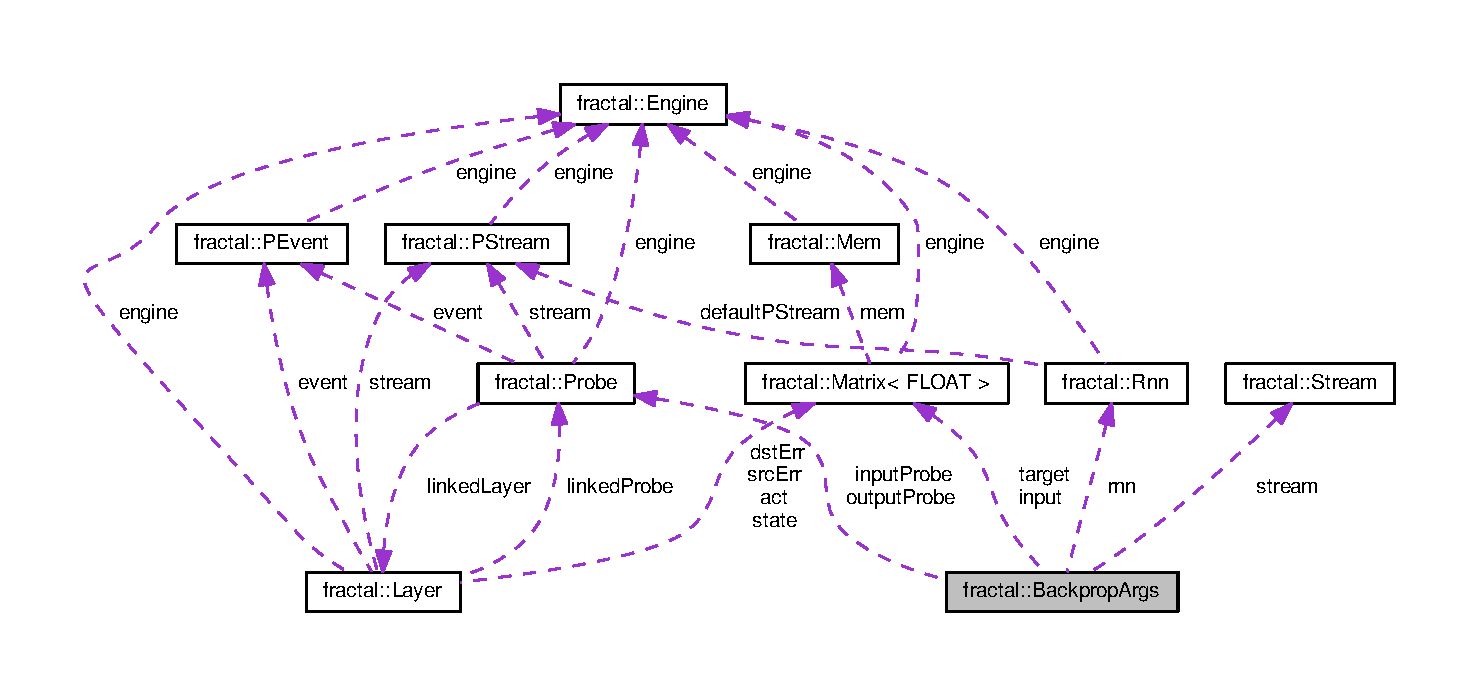
\includegraphics[width=350pt]{db/d39/classfractal_1_1BackpropArgs__coll__graph}
\end{center}
\end{figure}
\subsection*{Public Attributes}
\begin{DoxyCompactItemize}
\item 
\hyperlink{classfractal_1_1Rnn}{Rnn} $\ast$ \hyperlink{classfractal_1_1BackpropArgs_a97feb3d265db3976066700f99b657e42}{rnn}
\item 
\hyperlink{classfractal_1_1Stream}{Stream} $\ast$ \hyperlink{classfractal_1_1BackpropArgs_a16eae72910a2734b8857e02dbd15f06e}{stream}
\item 
unsigned long \hyperlink{classfractal_1_1BackpropArgs_ad9048cb8bd18097e49b46ab0bd7e7a76}{num\+Frame}
\item 
unsigned long \hyperlink{classfractal_1_1BackpropArgs_a3c715a926b61b851683280a0fd14c6b8}{n\+Stream}
\item 
unsigned long \hyperlink{classfractal_1_1BackpropArgs_ae346e9a842f88c30daa10d6edbc30bf4}{batch\+Size}
\item 
unsigned long \hyperlink{classfractal_1_1BackpropArgs_ae78c53109f97e43a3f4b167e6b562653}{frame\+Step}
\item 
unsigned long \hyperlink{classfractal_1_1BackpropArgs_a739d6ed1aa4132bd9fb18606fa1e1a17}{n\+Input}
\item 
unsigned long \hyperlink{classfractal_1_1BackpropArgs_a7b30c33f1ae37ce7e3b193a1560a292d}{n\+Output}
\item 
\hyperlink{classfractal_1_1Probe}{Probe} $\ast$ \hyperlink{classfractal_1_1BackpropArgs_a18a7ad6ff596d8f16388dae85d07794c}{input\+Probe}
\item 
\hyperlink{classfractal_1_1Probe}{Probe} $\ast$ \hyperlink{classfractal_1_1BackpropArgs_ae073c7cdaf8f81c9b634ce52e1bcf69a}{output\+Probe}
\item 
unsigned long $\ast$ \hyperlink{classfractal_1_1BackpropArgs_a054d628aec63cc312e2e211406fefd69}{input\+Channel}
\item 
unsigned long $\ast$ \hyperlink{classfractal_1_1BackpropArgs_aba9fc480f23686a563ceae2889660c23}{output\+Channel}
\item 
\hyperlink{classfractal_1_1Matrix}{Matrix}$<$ \hyperlink{namespacefractal_a1c2d2530689575d5ccb56bae52af70d3}{F\+L\+O\+A\+T} $>$ $\ast$ \hyperlink{classfractal_1_1BackpropArgs_a4e54ce09681eabdfad307e202a352fe8}{input}
\item 
\hyperlink{classfractal_1_1Matrix}{Matrix}$<$ \hyperlink{namespacefractal_a1c2d2530689575d5ccb56bae52af70d3}{F\+L\+O\+A\+T} $>$ $\ast$ \hyperlink{classfractal_1_1BackpropArgs_a7940fb93db22188b97167905155fdc44}{target}
\end{DoxyCompactItemize}


\subsection{Detailed Description}


Definition at line 31 of file Optimizer.\+h.



\subsection{Member Data Documentation}
\hypertarget{classfractal_1_1BackpropArgs_ae346e9a842f88c30daa10d6edbc30bf4}{\index{fractal\+::\+Backprop\+Args@{fractal\+::\+Backprop\+Args}!batch\+Size@{batch\+Size}}
\index{batch\+Size@{batch\+Size}!fractal\+::\+Backprop\+Args@{fractal\+::\+Backprop\+Args}}
\subsubsection[{batch\+Size}]{\setlength{\rightskip}{0pt plus 5cm}unsigned long fractal\+::\+Backprop\+Args\+::batch\+Size}}\label{classfractal_1_1BackpropArgs_ae346e9a842f88c30daa10d6edbc30bf4}


Definition at line 39 of file Optimizer.\+h.

\hypertarget{classfractal_1_1BackpropArgs_ae78c53109f97e43a3f4b167e6b562653}{\index{fractal\+::\+Backprop\+Args@{fractal\+::\+Backprop\+Args}!frame\+Step@{frame\+Step}}
\index{frame\+Step@{frame\+Step}!fractal\+::\+Backprop\+Args@{fractal\+::\+Backprop\+Args}}
\subsubsection[{frame\+Step}]{\setlength{\rightskip}{0pt plus 5cm}unsigned long fractal\+::\+Backprop\+Args\+::frame\+Step}}\label{classfractal_1_1BackpropArgs_ae78c53109f97e43a3f4b167e6b562653}


Definition at line 40 of file Optimizer.\+h.

\hypertarget{classfractal_1_1BackpropArgs_a4e54ce09681eabdfad307e202a352fe8}{\index{fractal\+::\+Backprop\+Args@{fractal\+::\+Backprop\+Args}!input@{input}}
\index{input@{input}!fractal\+::\+Backprop\+Args@{fractal\+::\+Backprop\+Args}}
\subsubsection[{input}]{\setlength{\rightskip}{0pt plus 5cm}{\bf Matrix}$<${\bf F\+L\+O\+A\+T}$>$$\ast$ fractal\+::\+Backprop\+Args\+::input}}\label{classfractal_1_1BackpropArgs_a4e54ce09681eabdfad307e202a352fe8}


Definition at line 50 of file Optimizer.\+h.

\hypertarget{classfractal_1_1BackpropArgs_a054d628aec63cc312e2e211406fefd69}{\index{fractal\+::\+Backprop\+Args@{fractal\+::\+Backprop\+Args}!input\+Channel@{input\+Channel}}
\index{input\+Channel@{input\+Channel}!fractal\+::\+Backprop\+Args@{fractal\+::\+Backprop\+Args}}
\subsubsection[{input\+Channel}]{\setlength{\rightskip}{0pt plus 5cm}unsigned long$\ast$ fractal\+::\+Backprop\+Args\+::input\+Channel}}\label{classfractal_1_1BackpropArgs_a054d628aec63cc312e2e211406fefd69}


Definition at line 47 of file Optimizer.\+h.

\hypertarget{classfractal_1_1BackpropArgs_a18a7ad6ff596d8f16388dae85d07794c}{\index{fractal\+::\+Backprop\+Args@{fractal\+::\+Backprop\+Args}!input\+Probe@{input\+Probe}}
\index{input\+Probe@{input\+Probe}!fractal\+::\+Backprop\+Args@{fractal\+::\+Backprop\+Args}}
\subsubsection[{input\+Probe}]{\setlength{\rightskip}{0pt plus 5cm}{\bf Probe}$\ast$ fractal\+::\+Backprop\+Args\+::input\+Probe}}\label{classfractal_1_1BackpropArgs_a18a7ad6ff596d8f16388dae85d07794c}


Definition at line 44 of file Optimizer.\+h.

\hypertarget{classfractal_1_1BackpropArgs_a739d6ed1aa4132bd9fb18606fa1e1a17}{\index{fractal\+::\+Backprop\+Args@{fractal\+::\+Backprop\+Args}!n\+Input@{n\+Input}}
\index{n\+Input@{n\+Input}!fractal\+::\+Backprop\+Args@{fractal\+::\+Backprop\+Args}}
\subsubsection[{n\+Input}]{\setlength{\rightskip}{0pt plus 5cm}unsigned long fractal\+::\+Backprop\+Args\+::n\+Input}}\label{classfractal_1_1BackpropArgs_a739d6ed1aa4132bd9fb18606fa1e1a17}


Definition at line 41 of file Optimizer.\+h.

\hypertarget{classfractal_1_1BackpropArgs_a7b30c33f1ae37ce7e3b193a1560a292d}{\index{fractal\+::\+Backprop\+Args@{fractal\+::\+Backprop\+Args}!n\+Output@{n\+Output}}
\index{n\+Output@{n\+Output}!fractal\+::\+Backprop\+Args@{fractal\+::\+Backprop\+Args}}
\subsubsection[{n\+Output}]{\setlength{\rightskip}{0pt plus 5cm}unsigned long fractal\+::\+Backprop\+Args\+::n\+Output}}\label{classfractal_1_1BackpropArgs_a7b30c33f1ae37ce7e3b193a1560a292d}


Definition at line 42 of file Optimizer.\+h.

\hypertarget{classfractal_1_1BackpropArgs_a3c715a926b61b851683280a0fd14c6b8}{\index{fractal\+::\+Backprop\+Args@{fractal\+::\+Backprop\+Args}!n\+Stream@{n\+Stream}}
\index{n\+Stream@{n\+Stream}!fractal\+::\+Backprop\+Args@{fractal\+::\+Backprop\+Args}}
\subsubsection[{n\+Stream}]{\setlength{\rightskip}{0pt plus 5cm}unsigned long fractal\+::\+Backprop\+Args\+::n\+Stream}}\label{classfractal_1_1BackpropArgs_a3c715a926b61b851683280a0fd14c6b8}


Definition at line 38 of file Optimizer.\+h.

\hypertarget{classfractal_1_1BackpropArgs_ad9048cb8bd18097e49b46ab0bd7e7a76}{\index{fractal\+::\+Backprop\+Args@{fractal\+::\+Backprop\+Args}!num\+Frame@{num\+Frame}}
\index{num\+Frame@{num\+Frame}!fractal\+::\+Backprop\+Args@{fractal\+::\+Backprop\+Args}}
\subsubsection[{num\+Frame}]{\setlength{\rightskip}{0pt plus 5cm}unsigned long fractal\+::\+Backprop\+Args\+::num\+Frame}}\label{classfractal_1_1BackpropArgs_ad9048cb8bd18097e49b46ab0bd7e7a76}


Definition at line 37 of file Optimizer.\+h.

\hypertarget{classfractal_1_1BackpropArgs_aba9fc480f23686a563ceae2889660c23}{\index{fractal\+::\+Backprop\+Args@{fractal\+::\+Backprop\+Args}!output\+Channel@{output\+Channel}}
\index{output\+Channel@{output\+Channel}!fractal\+::\+Backprop\+Args@{fractal\+::\+Backprop\+Args}}
\subsubsection[{output\+Channel}]{\setlength{\rightskip}{0pt plus 5cm}unsigned long$\ast$ fractal\+::\+Backprop\+Args\+::output\+Channel}}\label{classfractal_1_1BackpropArgs_aba9fc480f23686a563ceae2889660c23}


Definition at line 48 of file Optimizer.\+h.

\hypertarget{classfractal_1_1BackpropArgs_ae073c7cdaf8f81c9b634ce52e1bcf69a}{\index{fractal\+::\+Backprop\+Args@{fractal\+::\+Backprop\+Args}!output\+Probe@{output\+Probe}}
\index{output\+Probe@{output\+Probe}!fractal\+::\+Backprop\+Args@{fractal\+::\+Backprop\+Args}}
\subsubsection[{output\+Probe}]{\setlength{\rightskip}{0pt plus 5cm}{\bf Probe}$\ast$ fractal\+::\+Backprop\+Args\+::output\+Probe}}\label{classfractal_1_1BackpropArgs_ae073c7cdaf8f81c9b634ce52e1bcf69a}


Definition at line 45 of file Optimizer.\+h.

\hypertarget{classfractal_1_1BackpropArgs_a97feb3d265db3976066700f99b657e42}{\index{fractal\+::\+Backprop\+Args@{fractal\+::\+Backprop\+Args}!rnn@{rnn}}
\index{rnn@{rnn}!fractal\+::\+Backprop\+Args@{fractal\+::\+Backprop\+Args}}
\subsubsection[{rnn}]{\setlength{\rightskip}{0pt plus 5cm}{\bf Rnn}$\ast$ fractal\+::\+Backprop\+Args\+::rnn}}\label{classfractal_1_1BackpropArgs_a97feb3d265db3976066700f99b657e42}


Definition at line 34 of file Optimizer.\+h.

\hypertarget{classfractal_1_1BackpropArgs_a16eae72910a2734b8857e02dbd15f06e}{\index{fractal\+::\+Backprop\+Args@{fractal\+::\+Backprop\+Args}!stream@{stream}}
\index{stream@{stream}!fractal\+::\+Backprop\+Args@{fractal\+::\+Backprop\+Args}}
\subsubsection[{stream}]{\setlength{\rightskip}{0pt plus 5cm}{\bf Stream}$\ast$ fractal\+::\+Backprop\+Args\+::stream}}\label{classfractal_1_1BackpropArgs_a16eae72910a2734b8857e02dbd15f06e}


Definition at line 35 of file Optimizer.\+h.

\hypertarget{classfractal_1_1BackpropArgs_a7940fb93db22188b97167905155fdc44}{\index{fractal\+::\+Backprop\+Args@{fractal\+::\+Backprop\+Args}!target@{target}}
\index{target@{target}!fractal\+::\+Backprop\+Args@{fractal\+::\+Backprop\+Args}}
\subsubsection[{target}]{\setlength{\rightskip}{0pt plus 5cm}{\bf Matrix}$<${\bf F\+L\+O\+A\+T}$>$$\ast$ fractal\+::\+Backprop\+Args\+::target}}\label{classfractal_1_1BackpropArgs_a7940fb93db22188b97167905155fdc44}


Definition at line 51 of file Optimizer.\+h.



The documentation for this class was generated from the following file\+:\begin{DoxyCompactItemize}
\item 
src/util/\hyperlink{Optimizer_8h}{Optimizer.\+h}\end{DoxyCompactItemize}

\hypertarget{classfractal_1_1ClassificationEvaluator}{\section{fractal\+:\+:Classification\+Evaluator Class Reference}
\label{classfractal_1_1ClassificationEvaluator}\index{fractal\+::\+Classification\+Evaluator@{fractal\+::\+Classification\+Evaluator}}
}


{\ttfamily \#include $<$Classification\+Evaluator.\+h$>$}



Inheritance diagram for fractal\+:\+:Classification\+Evaluator\+:\nopagebreak
\begin{figure}[H]
\begin{center}
\leavevmode
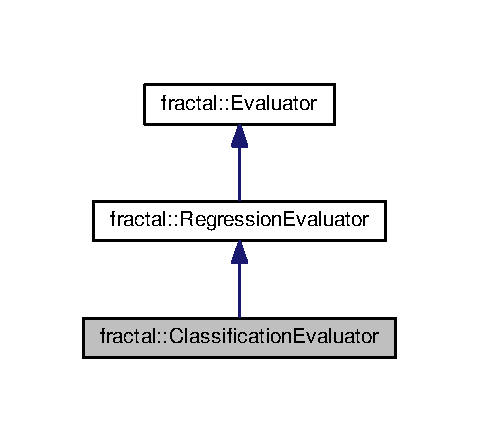
\includegraphics[width=230pt]{d6/ddb/classfractal_1_1ClassificationEvaluator__inherit__graph}
\end{center}
\end{figure}


Collaboration diagram for fractal\+:\+:Classification\+Evaluator\+:\nopagebreak
\begin{figure}[H]
\begin{center}
\leavevmode
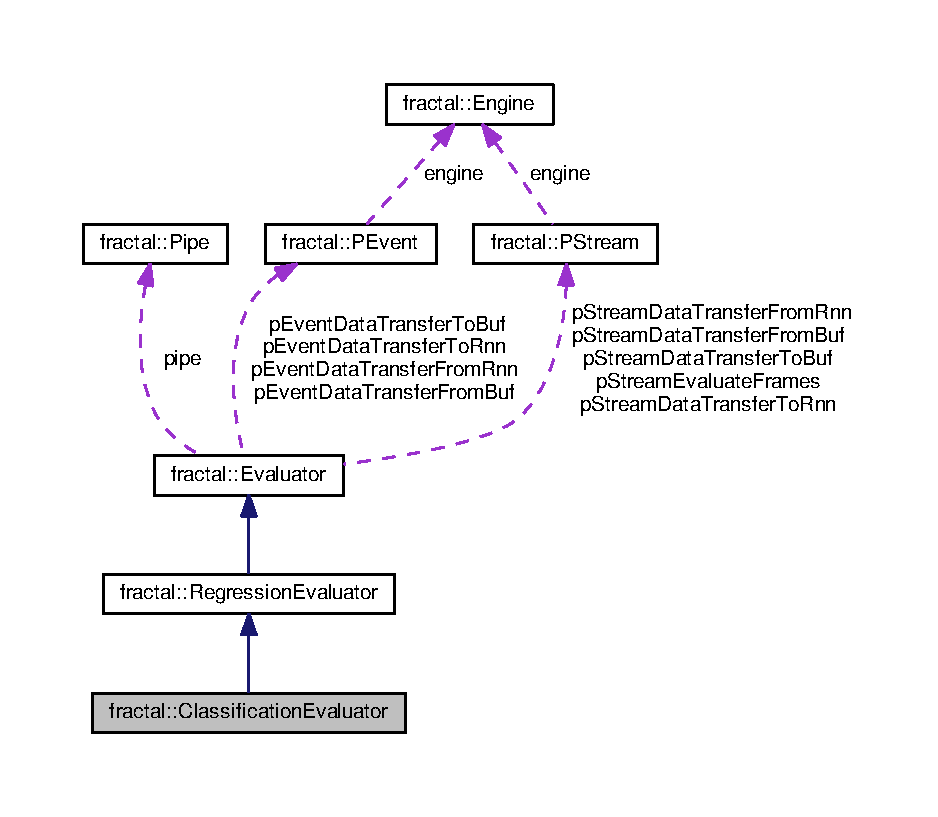
\includegraphics[width=350pt]{df/d5d/classfractal_1_1ClassificationEvaluator__coll__graph}
\end{center}
\end{figure}
\subsection*{Public Member Functions}
\begin{DoxyCompactItemize}
\item 
\hyperlink{classfractal_1_1ClassificationEvaluator_a6e0d5eac68626e054431dfc84cedf233}{Classification\+Evaluator} ()
\item 
virtual const double \hyperlink{classfractal_1_1ClassificationEvaluator_a15e9ad1d3e4c180729dd5bd07d4a6b78}{Get\+Loss} (const unsigned long output\+Idx) const 
\item 
const double \hyperlink{classfractal_1_1ClassificationEvaluator_ae0a157cb226de16be62a90491a3986c4}{Get\+Average\+Cross\+Entropy} (const unsigned long output\+Idx) const 
\item 
const double \hyperlink{classfractal_1_1ClassificationEvaluator_a07b4148d558449577463703022c4959a}{Get\+Frame\+Error\+Rate} (const unsigned long output\+Idx) const 
\item 
const unsigned long \hyperlink{classfractal_1_1ClassificationEvaluator_a4345f14ad53a36abe05627cb83c1a367}{Get\+Frame\+Error\+Count} (const unsigned long output\+Idx) const 
\end{DoxyCompactItemize}
\subsection*{Protected Member Functions}
\begin{DoxyCompactItemize}
\item 
virtual void \hyperlink{classfractal_1_1ClassificationEvaluator_a5bb2747a1915e12e6e0eec31fd857b84}{Reset} ()
\item 
virtual void \hyperlink{classfractal_1_1ClassificationEvaluator_a75e22cc1abbbeb16aa4d3e700fbe182c}{Evaluate\+Frames} (const unsigned long output\+Idx, \hyperlink{classfractal_1_1Matrix}{Matrix}$<$ \hyperlink{namespacefractal_a1c2d2530689575d5ccb56bae52af70d3}{F\+L\+O\+A\+T} $>$ \&target, \hyperlink{classfractal_1_1Matrix}{Matrix}$<$ \hyperlink{namespacefractal_a1c2d2530689575d5ccb56bae52af70d3}{F\+L\+O\+A\+T} $>$ \&output, const unsigned long n\+Stream, \hyperlink{classfractal_1_1PStream}{P\+Stream} \&stream)
\item 
virtual void \hyperlink{classfractal_1_1ClassificationEvaluator_aed4e92ea92c89ba01dd12cdde7215e70}{Mem\+Alloc} ()
\end{DoxyCompactItemize}
\subsection*{Protected Attributes}
\begin{DoxyCompactItemize}
\item 
std\+::vector$<$ unsigned long $>$ \hyperlink{classfractal_1_1ClassificationEvaluator_a3881e87f040fa426adb3f6e26d167b8b}{n\+Error}
\item 
std\+::vector$<$ double $>$ \hyperlink{classfractal_1_1ClassificationEvaluator_abea071ea947237bc9db18378509a1094}{ce\+Sum}
\end{DoxyCompactItemize}
\subsection*{Additional Inherited Members}


\subsection{Detailed Description}


Definition at line 28 of file Classification\+Evaluator.\+h.



\subsection{Constructor \& Destructor Documentation}
\hypertarget{classfractal_1_1ClassificationEvaluator_a6e0d5eac68626e054431dfc84cedf233}{\index{fractal\+::\+Classification\+Evaluator@{fractal\+::\+Classification\+Evaluator}!Classification\+Evaluator@{Classification\+Evaluator}}
\index{Classification\+Evaluator@{Classification\+Evaluator}!fractal\+::\+Classification\+Evaluator@{fractal\+::\+Classification\+Evaluator}}
\subsubsection[{Classification\+Evaluator}]{\setlength{\rightskip}{0pt plus 5cm}fractal\+::\+Classification\+Evaluator\+::\+Classification\+Evaluator (
\begin{DoxyParamCaption}
{}
\end{DoxyParamCaption}
)\hspace{0.3cm}{\ttfamily [inline]}}}\label{classfractal_1_1ClassificationEvaluator_a6e0d5eac68626e054431dfc84cedf233}


Definition at line 31 of file Classification\+Evaluator.\+h.



\subsection{Member Function Documentation}
\hypertarget{classfractal_1_1ClassificationEvaluator_a75e22cc1abbbeb16aa4d3e700fbe182c}{\index{fractal\+::\+Classification\+Evaluator@{fractal\+::\+Classification\+Evaluator}!Evaluate\+Frames@{Evaluate\+Frames}}
\index{Evaluate\+Frames@{Evaluate\+Frames}!fractal\+::\+Classification\+Evaluator@{fractal\+::\+Classification\+Evaluator}}
\subsubsection[{Evaluate\+Frames}]{\setlength{\rightskip}{0pt plus 5cm}void fractal\+::\+Classification\+Evaluator\+::\+Evaluate\+Frames (
\begin{DoxyParamCaption}
\item[{const unsigned long}]{output\+Idx, }
\item[{{\bf Matrix}$<$ {\bf F\+L\+O\+A\+T} $>$ \&}]{target, }
\item[{{\bf Matrix}$<$ {\bf F\+L\+O\+A\+T} $>$ \&}]{output, }
\item[{const unsigned long}]{n\+Stream, }
\item[{{\bf P\+Stream} \&}]{stream}
\end{DoxyParamCaption}
)\hspace{0.3cm}{\ttfamily [protected]}, {\ttfamily [virtual]}}}\label{classfractal_1_1ClassificationEvaluator_a75e22cc1abbbeb16aa4d3e700fbe182c}


Reimplemented from \hyperlink{classfractal_1_1RegressionEvaluator_ade117e7b38544fcee8c8a6518c7308b4}{fractal\+::\+Regression\+Evaluator}.



Definition at line 70 of file Classification\+Evaluator.\+cc.



Here is the call graph for this function\+:\nopagebreak
\begin{figure}[H]
\begin{center}
\leavevmode
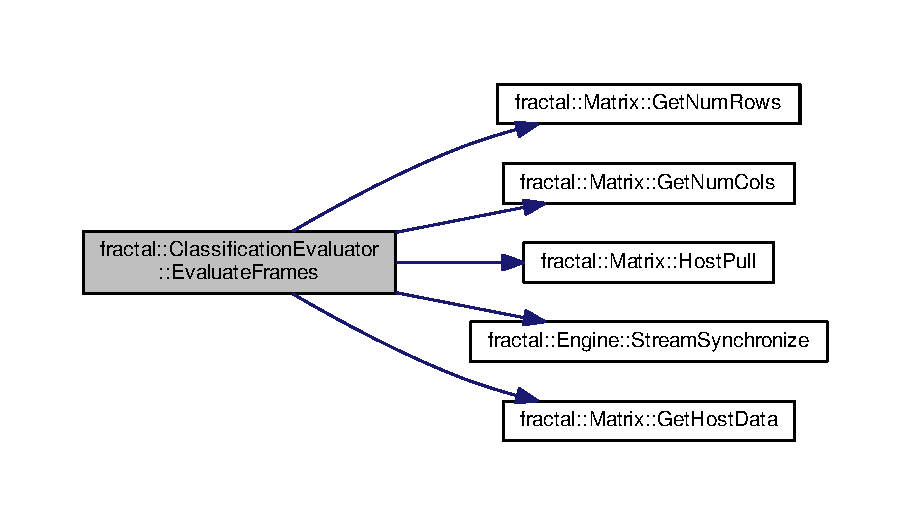
\includegraphics[width=350pt]{d2/d9c/classfractal_1_1ClassificationEvaluator_a75e22cc1abbbeb16aa4d3e700fbe182c_cgraph}
\end{center}
\end{figure}


\hypertarget{classfractal_1_1ClassificationEvaluator_ae0a157cb226de16be62a90491a3986c4}{\index{fractal\+::\+Classification\+Evaluator@{fractal\+::\+Classification\+Evaluator}!Get\+Average\+Cross\+Entropy@{Get\+Average\+Cross\+Entropy}}
\index{Get\+Average\+Cross\+Entropy@{Get\+Average\+Cross\+Entropy}!fractal\+::\+Classification\+Evaluator@{fractal\+::\+Classification\+Evaluator}}
\subsubsection[{Get\+Average\+Cross\+Entropy}]{\setlength{\rightskip}{0pt plus 5cm}const double fractal\+::\+Classification\+Evaluator\+::\+Get\+Average\+Cross\+Entropy (
\begin{DoxyParamCaption}
\item[{const unsigned long}]{output\+Idx}
\end{DoxyParamCaption}
) const}}\label{classfractal_1_1ClassificationEvaluator_ae0a157cb226de16be62a90491a3986c4}


Definition at line 32 of file Classification\+Evaluator.\+cc.



Here is the caller graph for this function\+:\nopagebreak
\begin{figure}[H]
\begin{center}
\leavevmode
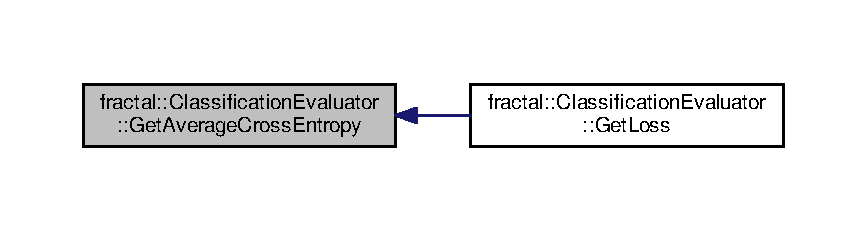
\includegraphics[width=350pt]{d2/d9c/classfractal_1_1ClassificationEvaluator_ae0a157cb226de16be62a90491a3986c4_icgraph}
\end{center}
\end{figure}


\hypertarget{classfractal_1_1ClassificationEvaluator_a4345f14ad53a36abe05627cb83c1a367}{\index{fractal\+::\+Classification\+Evaluator@{fractal\+::\+Classification\+Evaluator}!Get\+Frame\+Error\+Count@{Get\+Frame\+Error\+Count}}
\index{Get\+Frame\+Error\+Count@{Get\+Frame\+Error\+Count}!fractal\+::\+Classification\+Evaluator@{fractal\+::\+Classification\+Evaluator}}
\subsubsection[{Get\+Frame\+Error\+Count}]{\setlength{\rightskip}{0pt plus 5cm}const unsigned long fractal\+::\+Classification\+Evaluator\+::\+Get\+Frame\+Error\+Count (
\begin{DoxyParamCaption}
\item[{const unsigned long}]{output\+Idx}
\end{DoxyParamCaption}
) const}}\label{classfractal_1_1ClassificationEvaluator_a4345f14ad53a36abe05627cb83c1a367}


Definition at line 48 of file Classification\+Evaluator.\+cc.

\hypertarget{classfractal_1_1ClassificationEvaluator_a07b4148d558449577463703022c4959a}{\index{fractal\+::\+Classification\+Evaluator@{fractal\+::\+Classification\+Evaluator}!Get\+Frame\+Error\+Rate@{Get\+Frame\+Error\+Rate}}
\index{Get\+Frame\+Error\+Rate@{Get\+Frame\+Error\+Rate}!fractal\+::\+Classification\+Evaluator@{fractal\+::\+Classification\+Evaluator}}
\subsubsection[{Get\+Frame\+Error\+Rate}]{\setlength{\rightskip}{0pt plus 5cm}const double fractal\+::\+Classification\+Evaluator\+::\+Get\+Frame\+Error\+Rate (
\begin{DoxyParamCaption}
\item[{const unsigned long}]{output\+Idx}
\end{DoxyParamCaption}
) const}}\label{classfractal_1_1ClassificationEvaluator_a07b4148d558449577463703022c4959a}


Definition at line 40 of file Classification\+Evaluator.\+cc.

\hypertarget{classfractal_1_1ClassificationEvaluator_a15e9ad1d3e4c180729dd5bd07d4a6b78}{\index{fractal\+::\+Classification\+Evaluator@{fractal\+::\+Classification\+Evaluator}!Get\+Loss@{Get\+Loss}}
\index{Get\+Loss@{Get\+Loss}!fractal\+::\+Classification\+Evaluator@{fractal\+::\+Classification\+Evaluator}}
\subsubsection[{Get\+Loss}]{\setlength{\rightskip}{0pt plus 5cm}const double fractal\+::\+Classification\+Evaluator\+::\+Get\+Loss (
\begin{DoxyParamCaption}
\item[{const unsigned long}]{output\+Idx}
\end{DoxyParamCaption}
) const\hspace{0.3cm}{\ttfamily [virtual]}}}\label{classfractal_1_1ClassificationEvaluator_a15e9ad1d3e4c180729dd5bd07d4a6b78}


Reimplemented from \hyperlink{classfractal_1_1RegressionEvaluator_ab1b2e523dfb7a9886f9637541670b3e7}{fractal\+::\+Regression\+Evaluator}.



Definition at line 26 of file Classification\+Evaluator.\+cc.



Here is the call graph for this function\+:\nopagebreak
\begin{figure}[H]
\begin{center}
\leavevmode
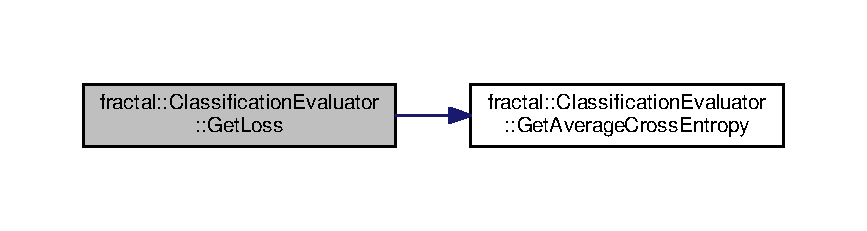
\includegraphics[width=350pt]{d2/d9c/classfractal_1_1ClassificationEvaluator_a15e9ad1d3e4c180729dd5bd07d4a6b78_cgraph}
\end{center}
\end{figure}


\hypertarget{classfractal_1_1ClassificationEvaluator_aed4e92ea92c89ba01dd12cdde7215e70}{\index{fractal\+::\+Classification\+Evaluator@{fractal\+::\+Classification\+Evaluator}!Mem\+Alloc@{Mem\+Alloc}}
\index{Mem\+Alloc@{Mem\+Alloc}!fractal\+::\+Classification\+Evaluator@{fractal\+::\+Classification\+Evaluator}}
\subsubsection[{Mem\+Alloc}]{\setlength{\rightskip}{0pt plus 5cm}void fractal\+::\+Classification\+Evaluator\+::\+Mem\+Alloc (
\begin{DoxyParamCaption}
{}
\end{DoxyParamCaption}
)\hspace{0.3cm}{\ttfamily [protected]}, {\ttfamily [virtual]}}}\label{classfractal_1_1ClassificationEvaluator_aed4e92ea92c89ba01dd12cdde7215e70}


Reimplemented from \hyperlink{classfractal_1_1RegressionEvaluator_ac2c59ad7a08a7a86b2d1b5585dd725c2}{fractal\+::\+Regression\+Evaluator}.



Definition at line 148 of file Classification\+Evaluator.\+cc.



Here is the call graph for this function\+:\nopagebreak
\begin{figure}[H]
\begin{center}
\leavevmode
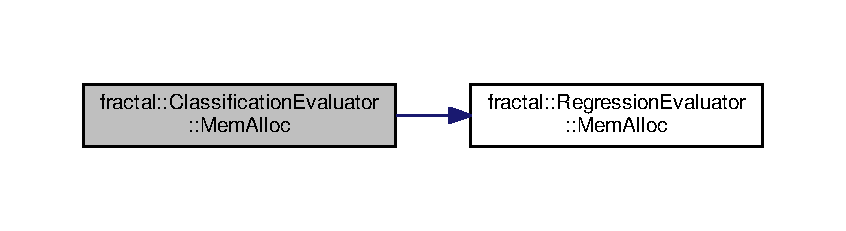
\includegraphics[width=350pt]{d2/d9c/classfractal_1_1ClassificationEvaluator_aed4e92ea92c89ba01dd12cdde7215e70_cgraph}
\end{center}
\end{figure}


\hypertarget{classfractal_1_1ClassificationEvaluator_a5bb2747a1915e12e6e0eec31fd857b84}{\index{fractal\+::\+Classification\+Evaluator@{fractal\+::\+Classification\+Evaluator}!Reset@{Reset}}
\index{Reset@{Reset}!fractal\+::\+Classification\+Evaluator@{fractal\+::\+Classification\+Evaluator}}
\subsubsection[{Reset}]{\setlength{\rightskip}{0pt plus 5cm}void fractal\+::\+Classification\+Evaluator\+::\+Reset (
\begin{DoxyParamCaption}
{}
\end{DoxyParamCaption}
)\hspace{0.3cm}{\ttfamily [protected]}, {\ttfamily [virtual]}}}\label{classfractal_1_1ClassificationEvaluator_a5bb2747a1915e12e6e0eec31fd857b84}


Reimplemented from \hyperlink{classfractal_1_1RegressionEvaluator_a3e7c99c111583353ae5a1ccb76cb86db}{fractal\+::\+Regression\+Evaluator}.



Definition at line 56 of file Classification\+Evaluator.\+cc.



Here is the call graph for this function\+:\nopagebreak
\begin{figure}[H]
\begin{center}
\leavevmode
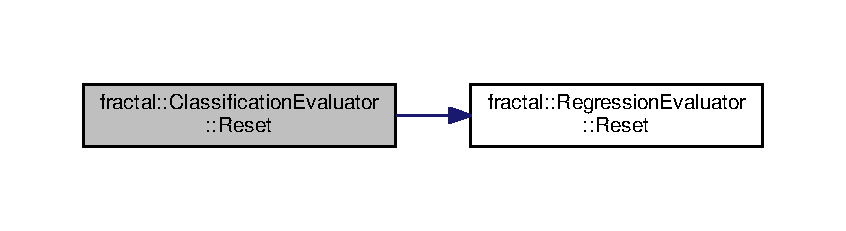
\includegraphics[width=350pt]{d2/d9c/classfractal_1_1ClassificationEvaluator_a5bb2747a1915e12e6e0eec31fd857b84_cgraph}
\end{center}
\end{figure}




\subsection{Member Data Documentation}
\hypertarget{classfractal_1_1ClassificationEvaluator_abea071ea947237bc9db18378509a1094}{\index{fractal\+::\+Classification\+Evaluator@{fractal\+::\+Classification\+Evaluator}!ce\+Sum@{ce\+Sum}}
\index{ce\+Sum@{ce\+Sum}!fractal\+::\+Classification\+Evaluator@{fractal\+::\+Classification\+Evaluator}}
\subsubsection[{ce\+Sum}]{\setlength{\rightskip}{0pt plus 5cm}std\+::vector$<$double$>$ fractal\+::\+Classification\+Evaluator\+::ce\+Sum\hspace{0.3cm}{\ttfamily [protected]}}}\label{classfractal_1_1ClassificationEvaluator_abea071ea947237bc9db18378509a1094}


Definition at line 46 of file Classification\+Evaluator.\+h.

\hypertarget{classfractal_1_1ClassificationEvaluator_a3881e87f040fa426adb3f6e26d167b8b}{\index{fractal\+::\+Classification\+Evaluator@{fractal\+::\+Classification\+Evaluator}!n\+Error@{n\+Error}}
\index{n\+Error@{n\+Error}!fractal\+::\+Classification\+Evaluator@{fractal\+::\+Classification\+Evaluator}}
\subsubsection[{n\+Error}]{\setlength{\rightskip}{0pt plus 5cm}std\+::vector$<$unsigned long$>$ fractal\+::\+Classification\+Evaluator\+::n\+Error\hspace{0.3cm}{\ttfamily [protected]}}}\label{classfractal_1_1ClassificationEvaluator_a3881e87f040fa426adb3f6e26d167b8b}


Definition at line 45 of file Classification\+Evaluator.\+h.



The documentation for this class was generated from the following files\+:\begin{DoxyCompactItemize}
\item 
src/util/\hyperlink{ClassificationEvaluator_8h}{Classification\+Evaluator.\+h}\item 
src/util/\hyperlink{ClassificationEvaluator_8cc}{Classification\+Evaluator.\+cc}\end{DoxyCompactItemize}

\hypertarget{classfractal_1_1Connection}{\section{fractal\+:\+:Connection Class Reference}
\label{classfractal_1_1Connection}\index{fractal\+::\+Connection@{fractal\+::\+Connection}}
}


{\ttfamily \#include $<$Connection.\+h$>$}



Collaboration diagram for fractal\+:\+:Connection\+:\nopagebreak
\begin{figure}[H]
\begin{center}
\leavevmode
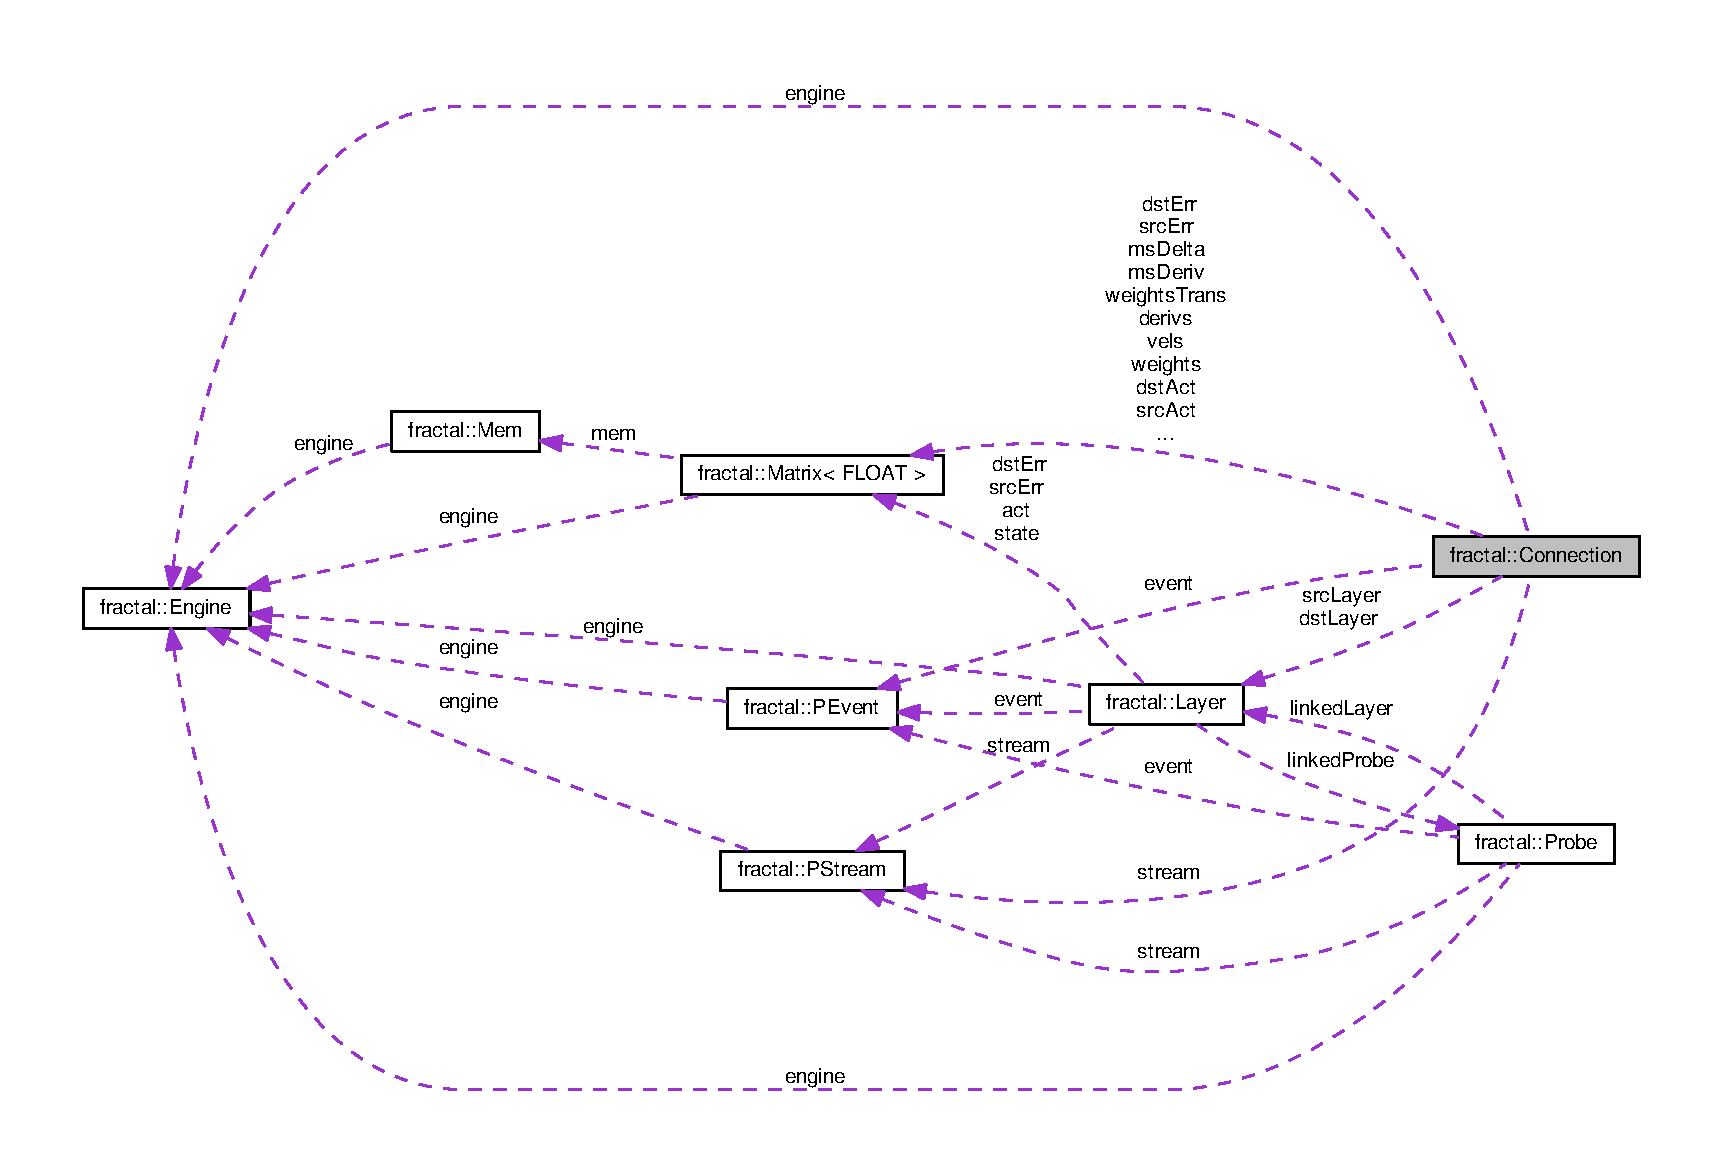
\includegraphics[width=350pt]{db/d34/classfractal_1_1Connection__coll__graph}
\end{center}
\end{figure}
\subsection*{Public Member Functions}
\begin{DoxyCompactItemize}
\item 
\hyperlink{classfractal_1_1Connection_a2e77dd8f37c2021d7b08fc012bdcd30c}{Connection} (\hyperlink{classfractal_1_1Layer}{Layer} $\ast$const from, \hyperlink{classfractal_1_1Layer}{Layer} $\ast$const to, const unsigned long \hyperlink{classfractal_1_1Connection_aeed56c0faa379d9c695e49457b63bc03}{delay\+Amount}, const bool is\+Identity)
\item 
virtual \hyperlink{classfractal_1_1Connection_a796fda5dd4b253c792d144ff483a0331}{$\sim$\+Connection} ()
\item 
void \hyperlink{classfractal_1_1Connection_a923b6313b13f60a464d417e638c4382b}{Set\+Engine} (\hyperlink{classfractal_1_1Engine}{Engine} $\ast$const \hyperlink{classfractal_1_1Connection_aed0a390a46ba6bcdff5c6238ac5b9bda}{engine}, \hyperlink{classfractal_1_1PStream}{P\+Stream} $\ast$const \hyperlink{classfractal_1_1Connection_afd1476955597e7a1fddb196fec69af82}{stream})
\item 
void \hyperlink{classfractal_1_1Connection_a09020f3027a886b7971baba901d8bf41}{Set\+Batch\+Size} (const unsigned long \hyperlink{classfractal_1_1Connection_a1c06df140701c272107c47b4ce40792b}{batch\+Size})
\item 
void \hyperlink{classfractal_1_1Connection_aab6dbd77374b404539f59d26d6c8f798}{Unlink\+Matrices} ()
\item 
void \hyperlink{classfractal_1_1Connection_a462d4925a2c205cf6c1640efe6b723be}{Init\+Weights} (const \hyperlink{classfractal_1_1InitWeightParam}{Init\+Weight\+Param} \&param)
\item 
void \hyperlink{classfractal_1_1Connection_a6beb3752a66f62f60238c22430486593}{Init\+Adadelta} (const \hyperlink{namespacefractal_a1c2d2530689575d5ccb56bae52af70d3}{F\+L\+O\+A\+T} decay\+Rate)
\item 
void \hyperlink{classfractal_1_1Connection_addddbba4b7044cad62a0541d26569f3b}{Init\+Nesterov} ()
\item 
void \hyperlink{classfractal_1_1Connection_a74c18a8efe61e4890c69b26063f74175}{Init\+Rmsprop} (const \hyperlink{namespacefractal_a1c2d2530689575d5ccb56bae52af70d3}{F\+L\+O\+A\+T} decay\+Rate)
\item 
void \hyperlink{classfractal_1_1Connection_a07f221e1751d01ed357b8bd4cc49dfbc}{Init\+Err} (const unsigned long batch\+From, const unsigned long batch\+To)
\item 
void \hyperlink{classfractal_1_1Connection_af95b3556c57e92edb06a4d33364dc0c2}{Forward} (const unsigned long batch\+From, const unsigned long batch\+To, const unsigned long n\+Stream)
\item 
void \hyperlink{classfractal_1_1Connection_af4754297e3aa7fcf27d68e7fc034d069}{Update\+Dst\+Err} (const unsigned long batch\+From, const unsigned long batch\+To)
\item 
void \hyperlink{classfractal_1_1Connection_a983f5ebf6c8072f950a0ca3c0bfdb6f1}{Backward} (const unsigned long batch\+From, const unsigned long batch\+To, const unsigned long n\+Stream)
\item 
void \hyperlink{classfractal_1_1Connection_a2b8a12fcdb97fe575d48348ac3e42daa}{Update\+Weights} (const unsigned long batch\+From, const unsigned long batch\+To, const unsigned long n\+Frame, const \hyperlink{namespacefractal_a1c2d2530689575d5ccb56bae52af70d3}{F\+L\+O\+A\+T} rate, const \hyperlink{namespacefractal_a1c2d2530689575d5ccb56bae52af70d3}{F\+L\+O\+A\+T} momentum, const bool adaptive\+Rates, const bool rmsprop)
\item 
const bool \hyperlink{classfractal_1_1Connection_a55a98b43749d2af37c492046bdabae30}{Is\+Delayed} () const 
\item 
const bool \hyperlink{classfractal_1_1Connection_a88b1bd4a69a9c1533ce0d2b261ad0825}{Is\+Identity} () const 
\item 
\hyperlink{classfractal_1_1Layer}{Layer} $\ast$const \hyperlink{classfractal_1_1Connection_a7ee554da75a227b017217121e9c0d70e}{Get\+Src\+Layer} () const 
\item 
\hyperlink{classfractal_1_1Layer}{Layer} $\ast$const \hyperlink{classfractal_1_1Connection_afeb565eb5cf7f0a86d78fb0b111eebc8}{Get\+Dst\+Layer} () const 
\item 
void \hyperlink{classfractal_1_1Connection_adf2811ab3189c8e4733b157486b26eb6}{Set\+P\+Stream} (\hyperlink{classfractal_1_1PStream}{P\+Stream} $\ast$const \hyperlink{classfractal_1_1Connection_afd1476955597e7a1fddb196fec69af82}{stream})
\item 
\hyperlink{classfractal_1_1PStream}{P\+Stream} \& \hyperlink{classfractal_1_1Connection_ad8d0ba5c34c518c24f3104448c5b0d6f}{Get\+P\+Stream} ()
\item 
void \hyperlink{classfractal_1_1Connection_a54577602a6deab30026078ce5a44f5cd}{Event\+Record} ()
\item 
void \hyperlink{classfractal_1_1Connection_a74c50d78f6c779d0a82a58f097fca3ef}{Stream\+Wait\+Event} (\hyperlink{classfractal_1_1PStream}{P\+Stream} \&\hyperlink{classfractal_1_1Connection_afd1476955597e7a1fddb196fec69af82}{stream})
\item 
void \hyperlink{classfractal_1_1Connection_a4ccde8145227156ce639a1c050ddb2a4}{Forward\+Wait} ()
\item 
void \hyperlink{classfractal_1_1Connection_aca0b898cc635378f3f246dfc6de384c6}{Backward\+Wait} ()
\item 
void \hyperlink{classfractal_1_1Connection_ae6c82dd4868442e324489ea88d12121d}{Save\+State} (const std\+::string \&filename)
\item 
void \hyperlink{classfractal_1_1Connection_a0539fa32a3eab1298eb7c373114fcc9e}{Load\+State} (const std\+::string \&filename)
\item 
const unsigned long \hyperlink{classfractal_1_1Connection_a8da7f0061214ed460eef30d18be2966d}{Get\+Num\+Weights} ()
\end{DoxyCompactItemize}
\subsection*{Protected Member Functions}
\begin{DoxyCompactItemize}
\item 
void \hyperlink{classfractal_1_1Connection_a9901894e4bd46fdcc7a8d8aa8c35b586}{Transpose\+Weight\+Matrix} ()
\end{DoxyCompactItemize}
\subsection*{Protected Attributes}
\begin{DoxyCompactItemize}
\item 
\hyperlink{classfractal_1_1Engine}{Engine} $\ast$ \hyperlink{classfractal_1_1Connection_aed0a390a46ba6bcdff5c6238ac5b9bda}{engine}
\item 
bool \hyperlink{classfractal_1_1Connection_aabe650cd29a9133e18de1a99bafd2069}{\+\_\+identity}
\item 
unsigned long \hyperlink{classfractal_1_1Connection_aeed56c0faa379d9c695e49457b63bc03}{delay\+Amount}
\item 
\hyperlink{classfractal_1_1Layer}{Layer} $\ast$ \hyperlink{classfractal_1_1Connection_a79a17a00d69083b24cd9ebcb11555952}{src\+Layer}
\item 
\hyperlink{classfractal_1_1Layer}{Layer} $\ast$ \hyperlink{classfractal_1_1Connection_a43d6bb6d604142602b3e339bb77bda33}{dst\+Layer}
\item 
unsigned long \hyperlink{classfractal_1_1Connection_a1c06df140701c272107c47b4ce40792b}{batch\+Size}
\item 
\hyperlink{namespacefractal_a1c2d2530689575d5ccb56bae52af70d3}{F\+L\+O\+A\+T} \hyperlink{classfractal_1_1Connection_ade0067c963f876032c92cd4198deaa32}{rms\+Decay\+Rate}
\item 
\hyperlink{classfractal_1_1Matrix}{Matrix}$<$ \hyperlink{namespacefractal_a1c2d2530689575d5ccb56bae52af70d3}{F\+L\+O\+A\+T} $>$ \hyperlink{classfractal_1_1Connection_a44f908ab921162e57108b5b6854e2ab0}{weights}
\item 
\hyperlink{classfractal_1_1Matrix}{Matrix}$<$ \hyperlink{namespacefractal_a1c2d2530689575d5ccb56bae52af70d3}{F\+L\+O\+A\+T} $>$ \hyperlink{classfractal_1_1Connection_a1df1793ca8ec947b29841138023e4ce7}{weights\+Trans}
\item 
bool \hyperlink{classfractal_1_1Connection_a22c55c2a935e38469f00cd7502d5bb0f}{weights\+Trans\+Valid}
\item 
\hyperlink{classfractal_1_1Matrix}{Matrix}$<$ \hyperlink{namespacefractal_a1c2d2530689575d5ccb56bae52af70d3}{F\+L\+O\+A\+T} $>$ \hyperlink{classfractal_1_1Connection_ae56d3a80cde5f872b18e11a9e087a335}{vels}
\item 
\hyperlink{classfractal_1_1Matrix}{Matrix}$<$ \hyperlink{namespacefractal_a1c2d2530689575d5ccb56bae52af70d3}{F\+L\+O\+A\+T} $>$ \hyperlink{classfractal_1_1Connection_a31f6cf9d89d0c4166dc8bde044fafd00}{derivs}
\item 
\hyperlink{classfractal_1_1Matrix}{Matrix}$<$ \hyperlink{namespacefractal_a1c2d2530689575d5ccb56bae52af70d3}{F\+L\+O\+A\+T} $>$ \hyperlink{classfractal_1_1Connection_ac4df1add96950e005f005047f25f158d}{ms\+Deriv}
\item 
\hyperlink{classfractal_1_1Matrix}{Matrix}$<$ \hyperlink{namespacefractal_a1c2d2530689575d5ccb56bae52af70d3}{F\+L\+O\+A\+T} $>$ \hyperlink{classfractal_1_1Connection_a0cd41b30d1dc0db0a6722521a20906ea}{ms\+Delta}
\item 
\hyperlink{classfractal_1_1Matrix}{Matrix}$<$ \hyperlink{namespacefractal_a1c2d2530689575d5ccb56bae52af70d3}{F\+L\+O\+A\+T} $>$ \hyperlink{classfractal_1_1Connection_a7e99d505ee81e3c7c00dceb70efdf8bf}{dst\+Act}
\item 
\hyperlink{classfractal_1_1Matrix}{Matrix}$<$ \hyperlink{namespacefractal_a1c2d2530689575d5ccb56bae52af70d3}{F\+L\+O\+A\+T} $>$ \hyperlink{classfractal_1_1Connection_aae995012548c5f535cf4dd16aa8985c5}{src\+Act}
\item 
\hyperlink{classfractal_1_1Matrix}{Matrix}$<$ \hyperlink{namespacefractal_a1c2d2530689575d5ccb56bae52af70d3}{F\+L\+O\+A\+T} $>$ \hyperlink{classfractal_1_1Connection_a2374b05f600966a36a1eec9b0946328d}{dst\+Err}
\item 
\hyperlink{classfractal_1_1Matrix}{Matrix}$<$ \hyperlink{namespacefractal_a1c2d2530689575d5ccb56bae52af70d3}{F\+L\+O\+A\+T} $>$ \hyperlink{classfractal_1_1Connection_abc00863a5dc0e43990ace905ed7f50c0}{src\+Err}
\item 
\hyperlink{classfractal_1_1PStream}{P\+Stream} $\ast$ \hyperlink{classfractal_1_1Connection_afd1476955597e7a1fddb196fec69af82}{stream}
\item 
\hyperlink{classfractal_1_1PEvent}{P\+Event} \hyperlink{classfractal_1_1Connection_a1440177a726771823d046340f1c24e59}{event}
\item 
friend \hyperlink{classfractal_1_1Connection_aee958063517851c72a62c55f049300be}{Layer}
\end{DoxyCompactItemize}


\subsection{Detailed Description}


Definition at line 36 of file Connection.\+h.



\subsection{Constructor \& Destructor Documentation}
\hypertarget{classfractal_1_1Connection_a2e77dd8f37c2021d7b08fc012bdcd30c}{\index{fractal\+::\+Connection@{fractal\+::\+Connection}!Connection@{Connection}}
\index{Connection@{Connection}!fractal\+::\+Connection@{fractal\+::\+Connection}}
\subsubsection[{Connection}]{\setlength{\rightskip}{0pt plus 5cm}fractal\+::\+Connection\+::\+Connection (
\begin{DoxyParamCaption}
\item[{{\bf Layer} $\ast$const}]{from, }
\item[{{\bf Layer} $\ast$const}]{to, }
\item[{const unsigned long}]{delay\+Amount, }
\item[{const bool}]{is\+Identity}
\end{DoxyParamCaption}
)}}\label{classfractal_1_1Connection_a2e77dd8f37c2021d7b08fc012bdcd30c}


Definition at line 29 of file Connection.\+cc.



Here is the call graph for this function\+:\nopagebreak
\begin{figure}[H]
\begin{center}
\leavevmode
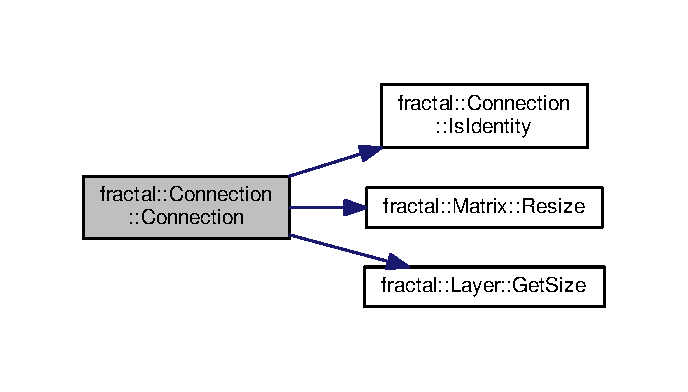
\includegraphics[width=330pt]{da/dbf/classfractal_1_1Connection_a2e77dd8f37c2021d7b08fc012bdcd30c_cgraph}
\end{center}
\end{figure}


\hypertarget{classfractal_1_1Connection_a796fda5dd4b253c792d144ff483a0331}{\index{fractal\+::\+Connection@{fractal\+::\+Connection}!````~Connection@{$\sim$\+Connection}}
\index{````~Connection@{$\sim$\+Connection}!fractal\+::\+Connection@{fractal\+::\+Connection}}
\subsubsection[{$\sim$\+Connection}]{\setlength{\rightskip}{0pt plus 5cm}fractal\+::\+Connection\+::$\sim$\+Connection (
\begin{DoxyParamCaption}
{}
\end{DoxyParamCaption}
)\hspace{0.3cm}{\ttfamily [virtual]}}}\label{classfractal_1_1Connection_a796fda5dd4b253c792d144ff483a0331}


Definition at line 54 of file Connection.\+cc.



Here is the call graph for this function\+:\nopagebreak
\begin{figure}[H]
\begin{center}
\leavevmode
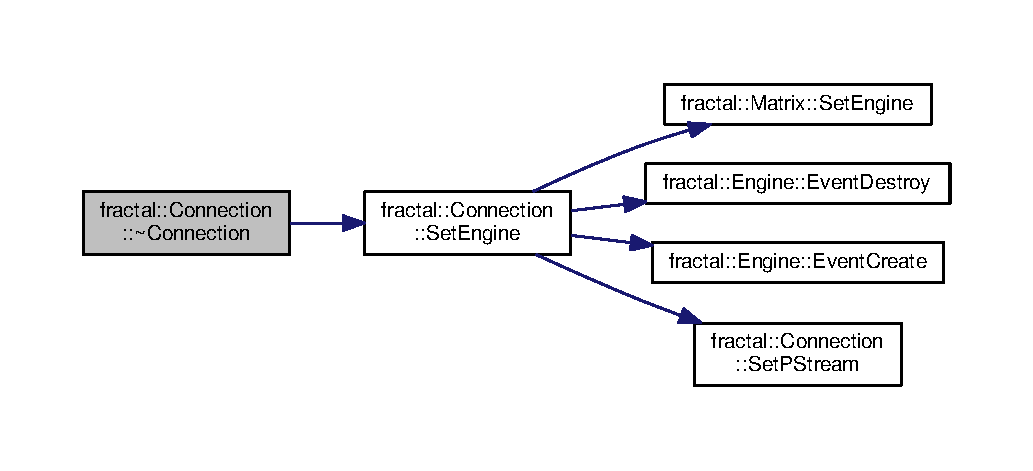
\includegraphics[width=350pt]{da/dbf/classfractal_1_1Connection_a796fda5dd4b253c792d144ff483a0331_cgraph}
\end{center}
\end{figure}




\subsection{Member Function Documentation}
\hypertarget{classfractal_1_1Connection_a983f5ebf6c8072f950a0ca3c0bfdb6f1}{\index{fractal\+::\+Connection@{fractal\+::\+Connection}!Backward@{Backward}}
\index{Backward@{Backward}!fractal\+::\+Connection@{fractal\+::\+Connection}}
\subsubsection[{Backward}]{\setlength{\rightskip}{0pt plus 5cm}void fractal\+::\+Connection\+::\+Backward (
\begin{DoxyParamCaption}
\item[{const unsigned long}]{batch\+From, }
\item[{const unsigned long}]{batch\+To, }
\item[{const unsigned long}]{n\+Stream}
\end{DoxyParamCaption}
)}}\label{classfractal_1_1Connection_a983f5ebf6c8072f950a0ca3c0bfdb6f1}


Definition at line 264 of file Connection.\+cc.



Here is the call graph for this function\+:\nopagebreak
\begin{figure}[H]
\begin{center}
\leavevmode
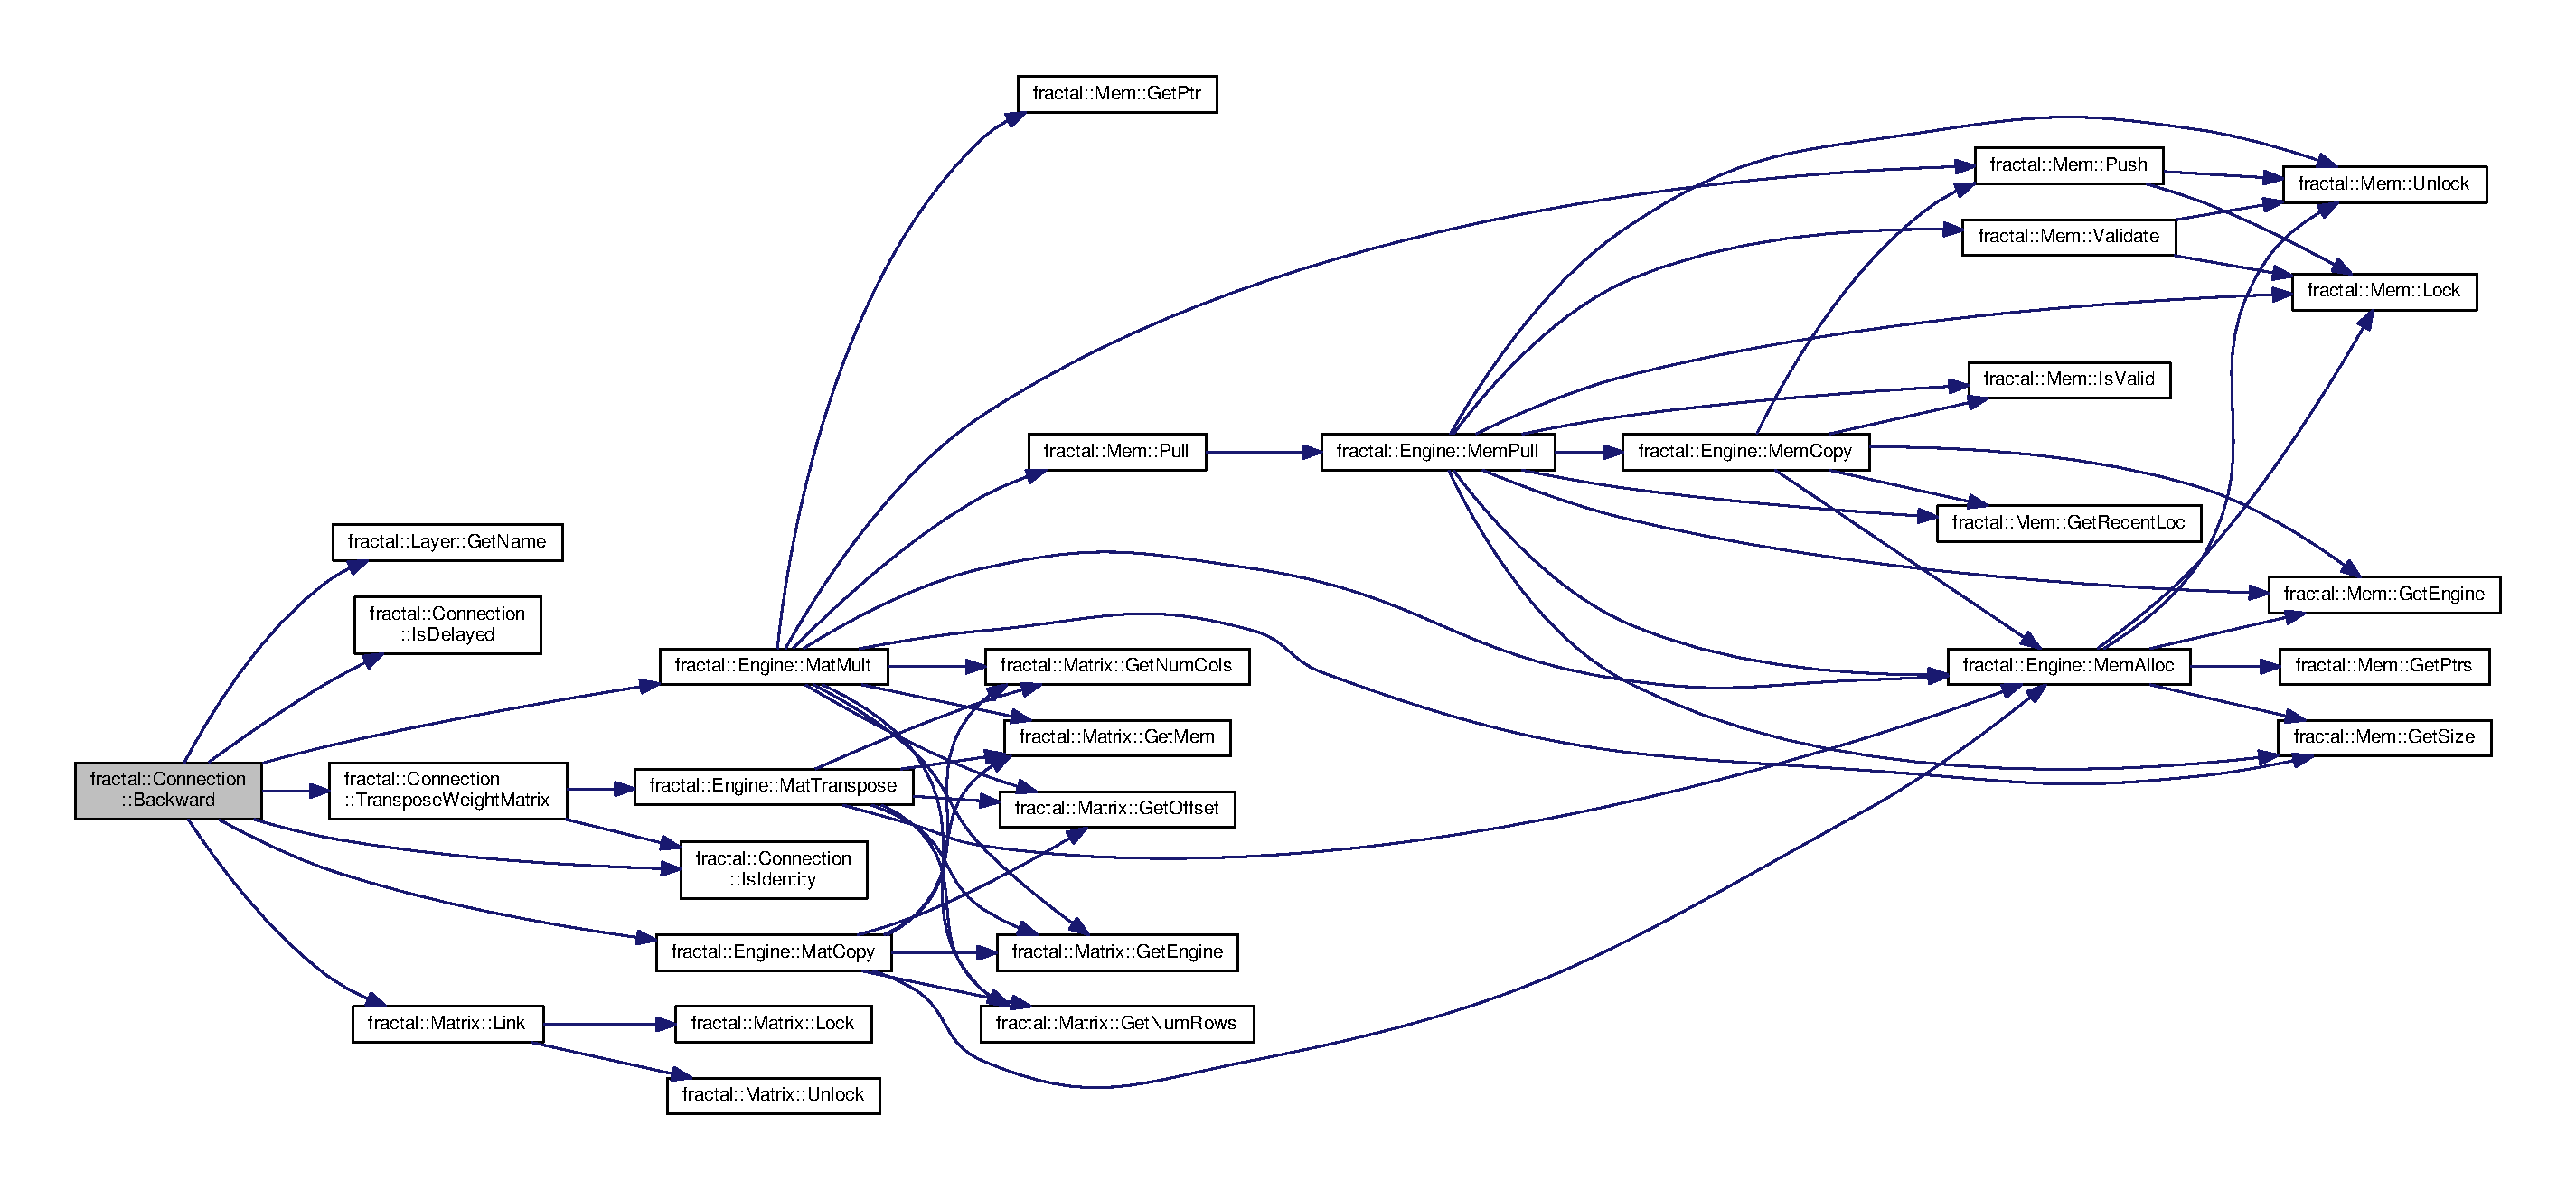
\includegraphics[width=350pt]{da/dbf/classfractal_1_1Connection_a983f5ebf6c8072f950a0ca3c0bfdb6f1_cgraph}
\end{center}
\end{figure}




Here is the caller graph for this function\+:\nopagebreak
\begin{figure}[H]
\begin{center}
\leavevmode
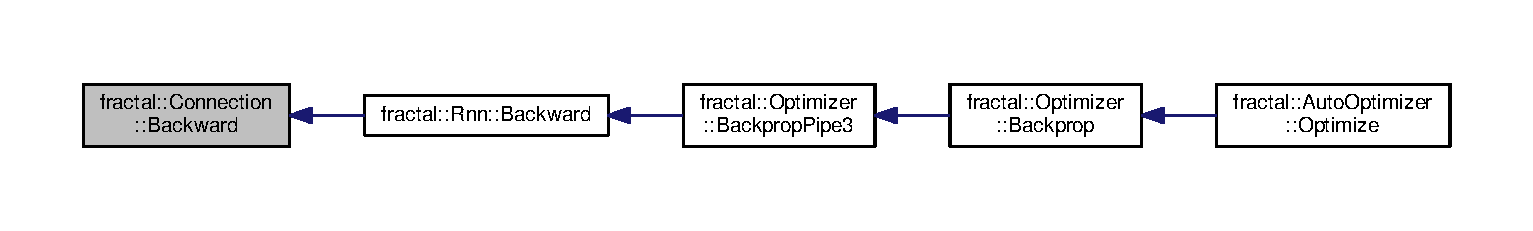
\includegraphics[width=350pt]{da/dbf/classfractal_1_1Connection_a983f5ebf6c8072f950a0ca3c0bfdb6f1_icgraph}
\end{center}
\end{figure}


\hypertarget{classfractal_1_1Connection_aca0b898cc635378f3f246dfc6de384c6}{\index{fractal\+::\+Connection@{fractal\+::\+Connection}!Backward\+Wait@{Backward\+Wait}}
\index{Backward\+Wait@{Backward\+Wait}!fractal\+::\+Connection@{fractal\+::\+Connection}}
\subsubsection[{Backward\+Wait}]{\setlength{\rightskip}{0pt plus 5cm}void fractal\+::\+Connection\+::\+Backward\+Wait (
\begin{DoxyParamCaption}
{}
\end{DoxyParamCaption}
)}}\label{classfractal_1_1Connection_aca0b898cc635378f3f246dfc6de384c6}


Definition at line 400 of file Connection.\+cc.



Here is the call graph for this function\+:\nopagebreak
\begin{figure}[H]
\begin{center}
\leavevmode
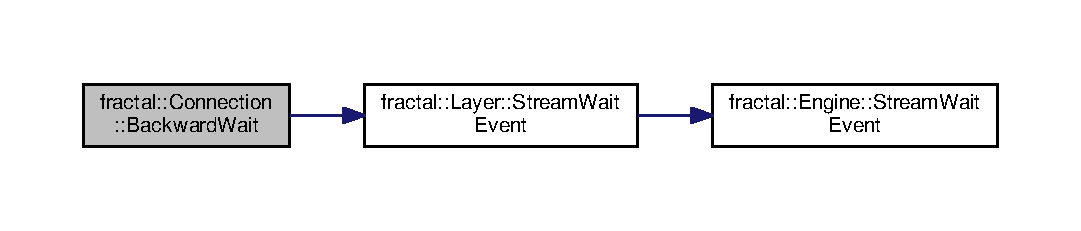
\includegraphics[width=350pt]{da/dbf/classfractal_1_1Connection_aca0b898cc635378f3f246dfc6de384c6_cgraph}
\end{center}
\end{figure}




Here is the caller graph for this function\+:\nopagebreak
\begin{figure}[H]
\begin{center}
\leavevmode
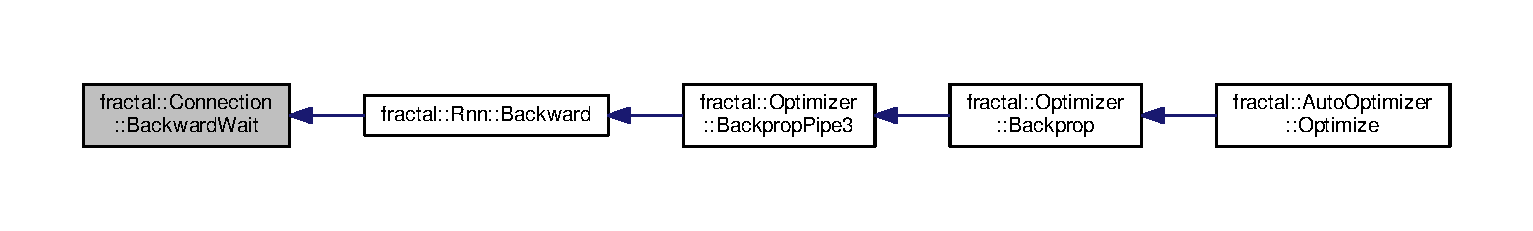
\includegraphics[width=350pt]{da/dbf/classfractal_1_1Connection_aca0b898cc635378f3f246dfc6de384c6_icgraph}
\end{center}
\end{figure}


\hypertarget{classfractal_1_1Connection_a54577602a6deab30026078ce5a44f5cd}{\index{fractal\+::\+Connection@{fractal\+::\+Connection}!Event\+Record@{Event\+Record}}
\index{Event\+Record@{Event\+Record}!fractal\+::\+Connection@{fractal\+::\+Connection}}
\subsubsection[{Event\+Record}]{\setlength{\rightskip}{0pt plus 5cm}void fractal\+::\+Connection\+::\+Event\+Record (
\begin{DoxyParamCaption}
{}
\end{DoxyParamCaption}
)}}\label{classfractal_1_1Connection_a54577602a6deab30026078ce5a44f5cd}


Definition at line 380 of file Connection.\+cc.



Here is the call graph for this function\+:\nopagebreak
\begin{figure}[H]
\begin{center}
\leavevmode
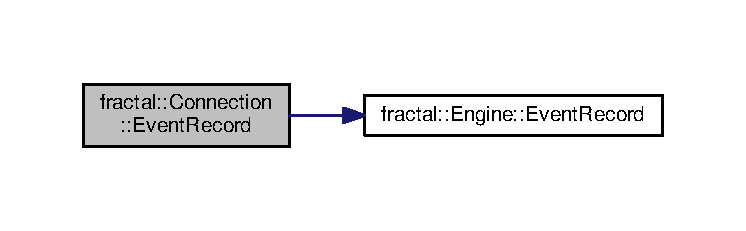
\includegraphics[width=350pt]{da/dbf/classfractal_1_1Connection_a54577602a6deab30026078ce5a44f5cd_cgraph}
\end{center}
\end{figure}




Here is the caller graph for this function\+:\nopagebreak
\begin{figure}[H]
\begin{center}
\leavevmode
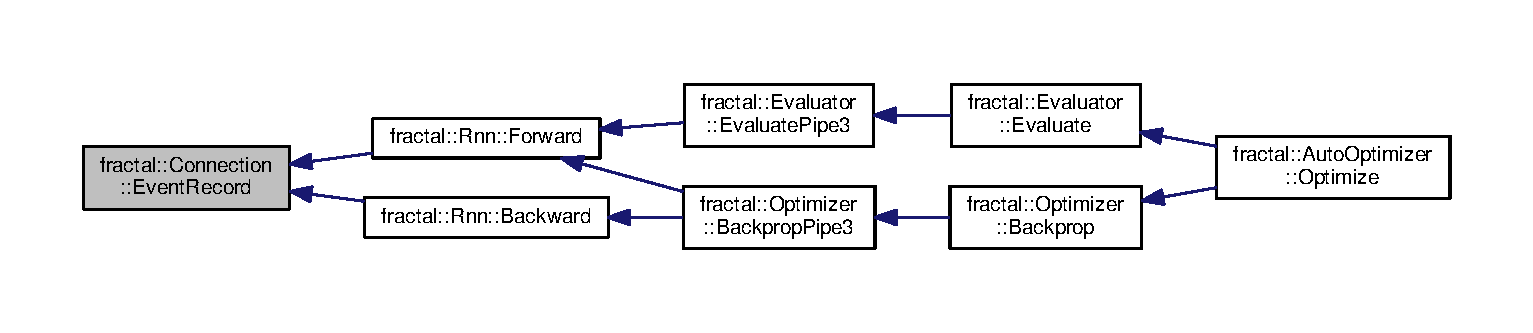
\includegraphics[width=350pt]{da/dbf/classfractal_1_1Connection_a54577602a6deab30026078ce5a44f5cd_icgraph}
\end{center}
\end{figure}


\hypertarget{classfractal_1_1Connection_af95b3556c57e92edb06a4d33364dc0c2}{\index{fractal\+::\+Connection@{fractal\+::\+Connection}!Forward@{Forward}}
\index{Forward@{Forward}!fractal\+::\+Connection@{fractal\+::\+Connection}}
\subsubsection[{Forward}]{\setlength{\rightskip}{0pt plus 5cm}void fractal\+::\+Connection\+::\+Forward (
\begin{DoxyParamCaption}
\item[{const unsigned long}]{batch\+From, }
\item[{const unsigned long}]{batch\+To, }
\item[{const unsigned long}]{n\+Stream}
\end{DoxyParamCaption}
)}}\label{classfractal_1_1Connection_af95b3556c57e92edb06a4d33364dc0c2}


Definition at line 195 of file Connection.\+cc.



Here is the call graph for this function\+:\nopagebreak
\begin{figure}[H]
\begin{center}
\leavevmode
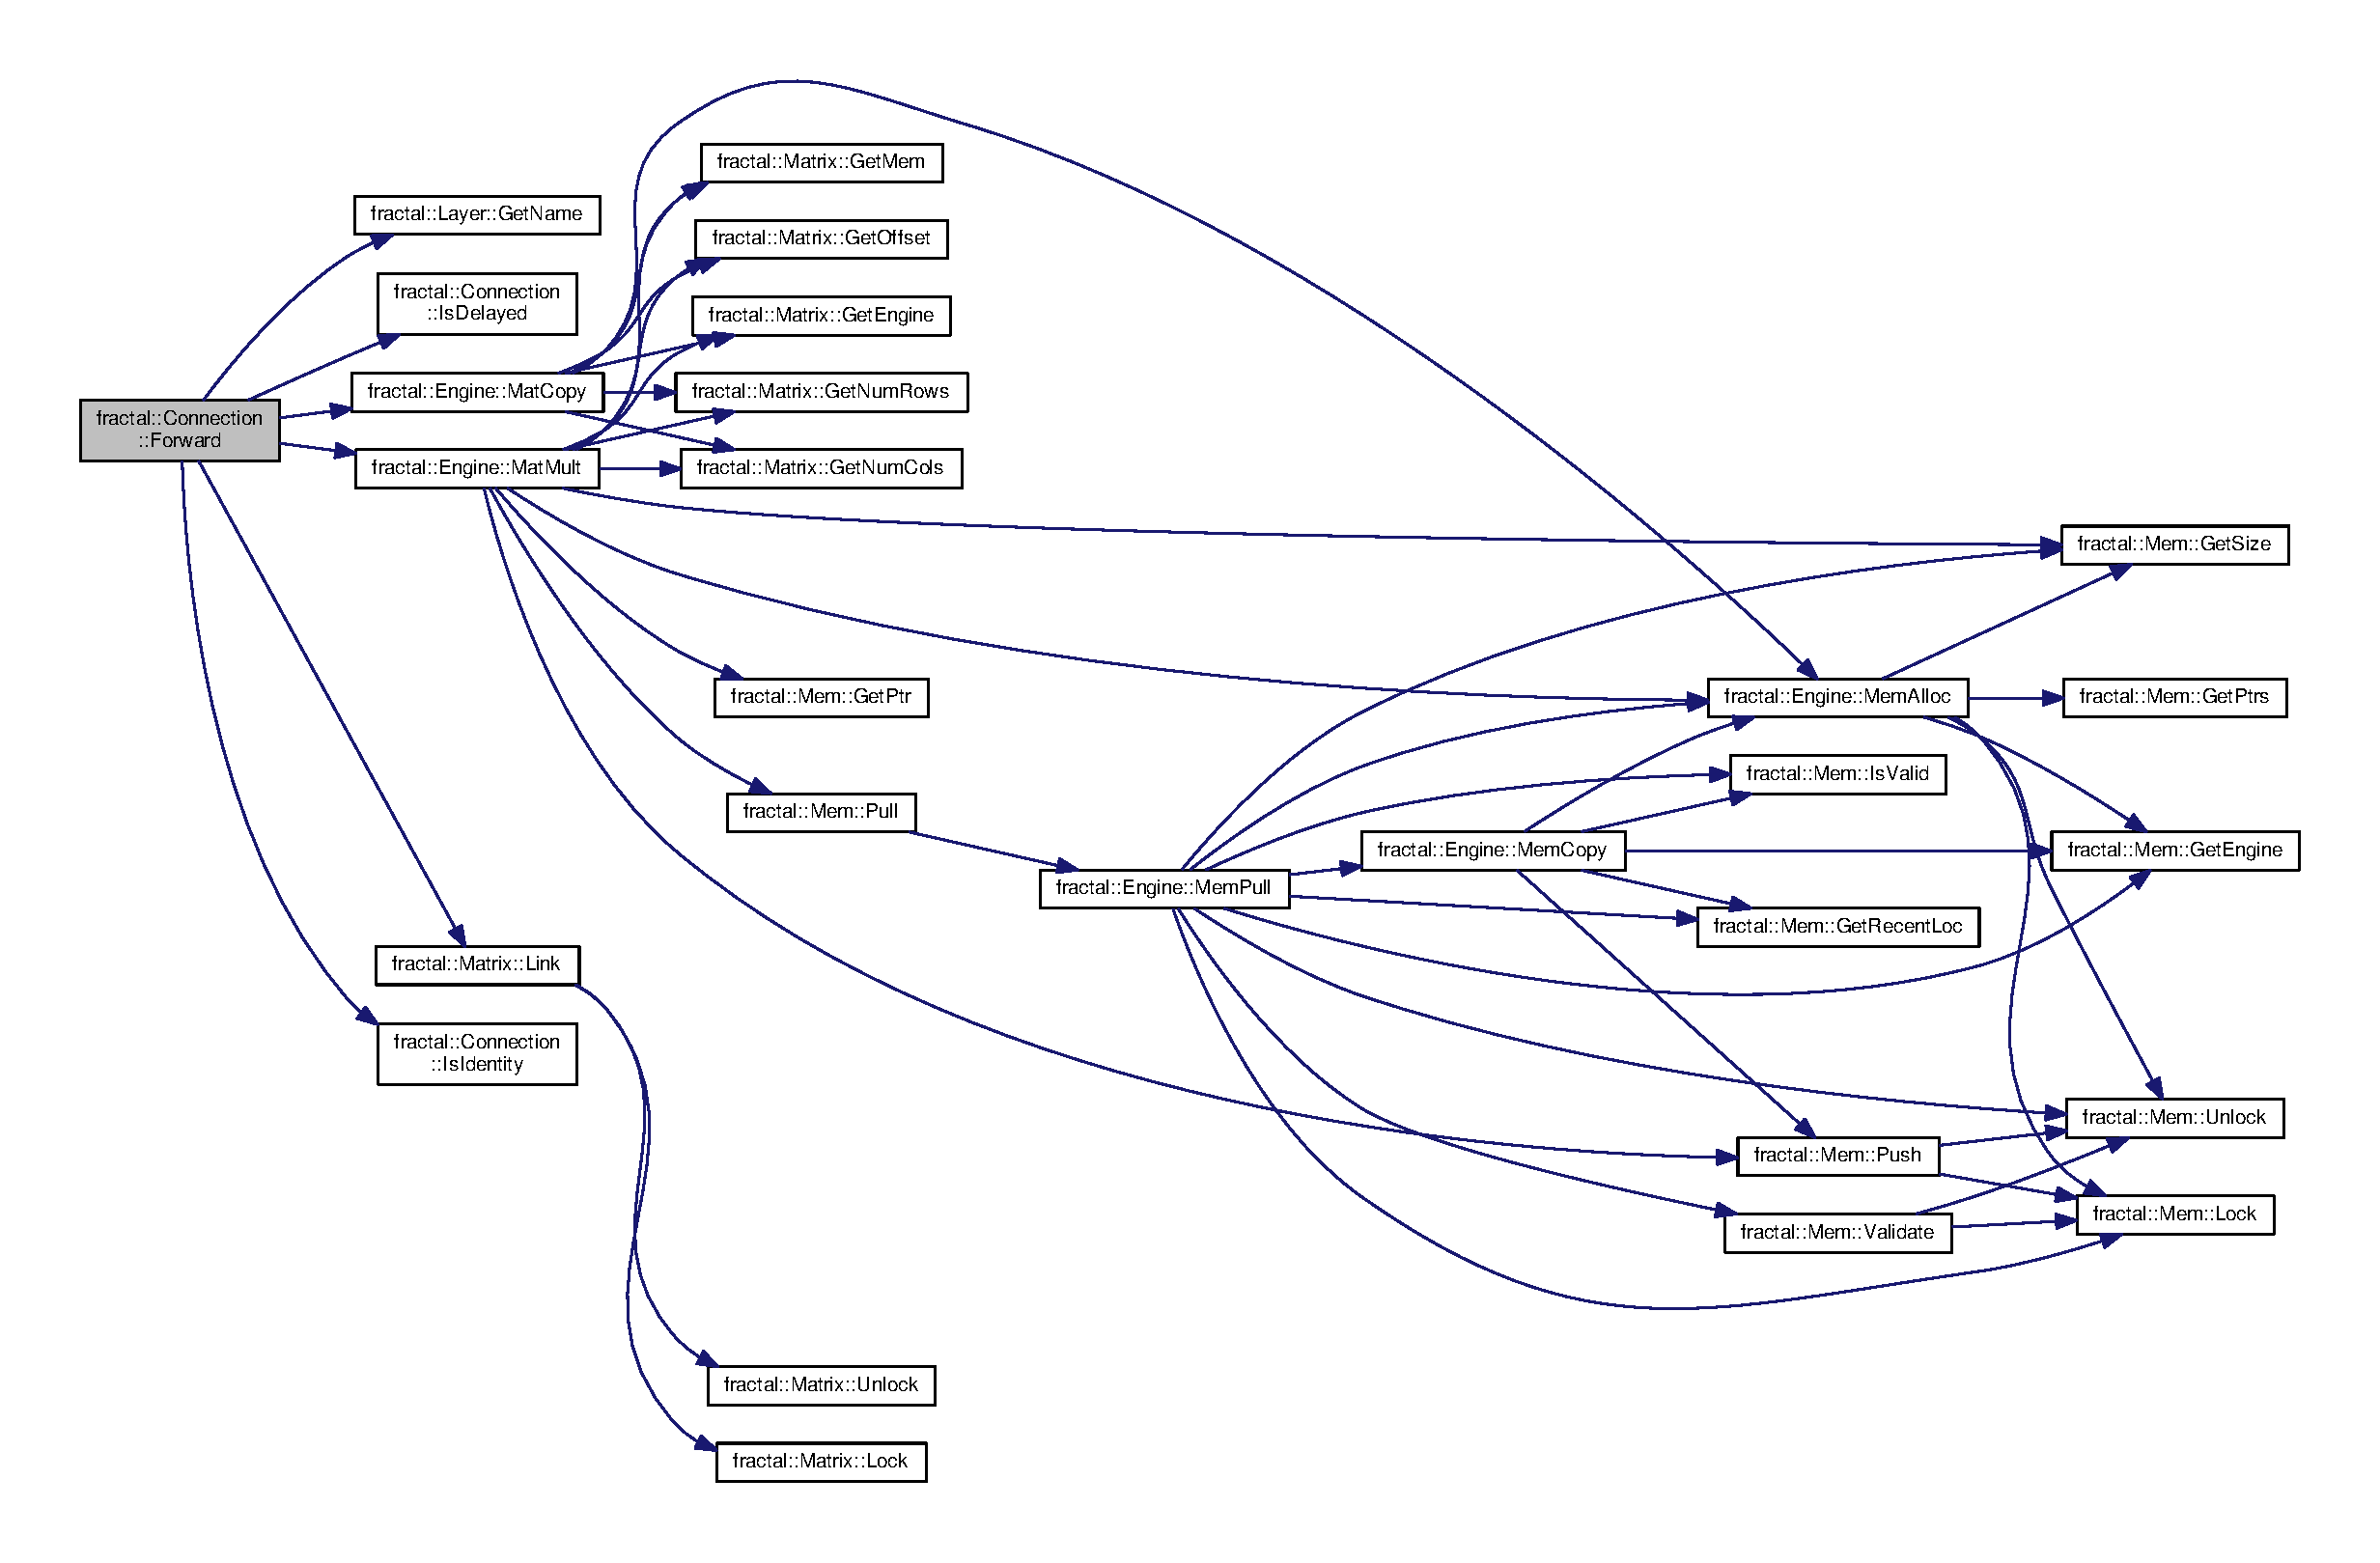
\includegraphics[width=350pt]{da/dbf/classfractal_1_1Connection_af95b3556c57e92edb06a4d33364dc0c2_cgraph}
\end{center}
\end{figure}




Here is the caller graph for this function\+:\nopagebreak
\begin{figure}[H]
\begin{center}
\leavevmode
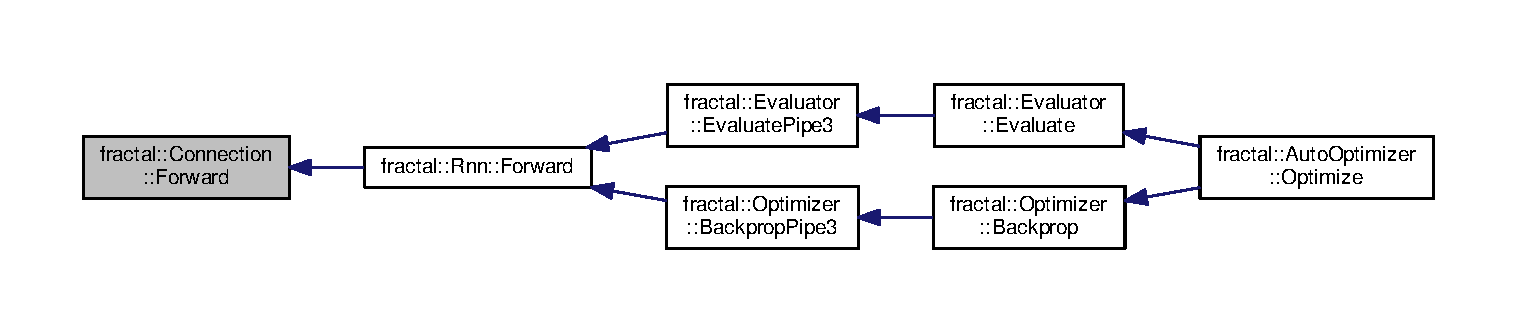
\includegraphics[width=350pt]{da/dbf/classfractal_1_1Connection_af95b3556c57e92edb06a4d33364dc0c2_icgraph}
\end{center}
\end{figure}


\hypertarget{classfractal_1_1Connection_a4ccde8145227156ce639a1c050ddb2a4}{\index{fractal\+::\+Connection@{fractal\+::\+Connection}!Forward\+Wait@{Forward\+Wait}}
\index{Forward\+Wait@{Forward\+Wait}!fractal\+::\+Connection@{fractal\+::\+Connection}}
\subsubsection[{Forward\+Wait}]{\setlength{\rightskip}{0pt plus 5cm}void fractal\+::\+Connection\+::\+Forward\+Wait (
\begin{DoxyParamCaption}
{}
\end{DoxyParamCaption}
)}}\label{classfractal_1_1Connection_a4ccde8145227156ce639a1c050ddb2a4}


Definition at line 394 of file Connection.\+cc.



Here is the call graph for this function\+:\nopagebreak
\begin{figure}[H]
\begin{center}
\leavevmode
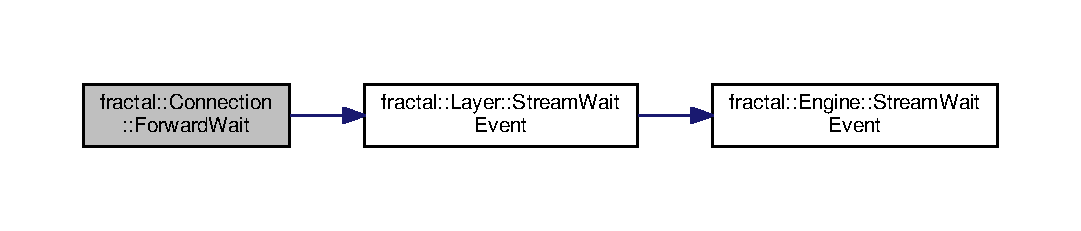
\includegraphics[width=350pt]{da/dbf/classfractal_1_1Connection_a4ccde8145227156ce639a1c050ddb2a4_cgraph}
\end{center}
\end{figure}




Here is the caller graph for this function\+:\nopagebreak
\begin{figure}[H]
\begin{center}
\leavevmode
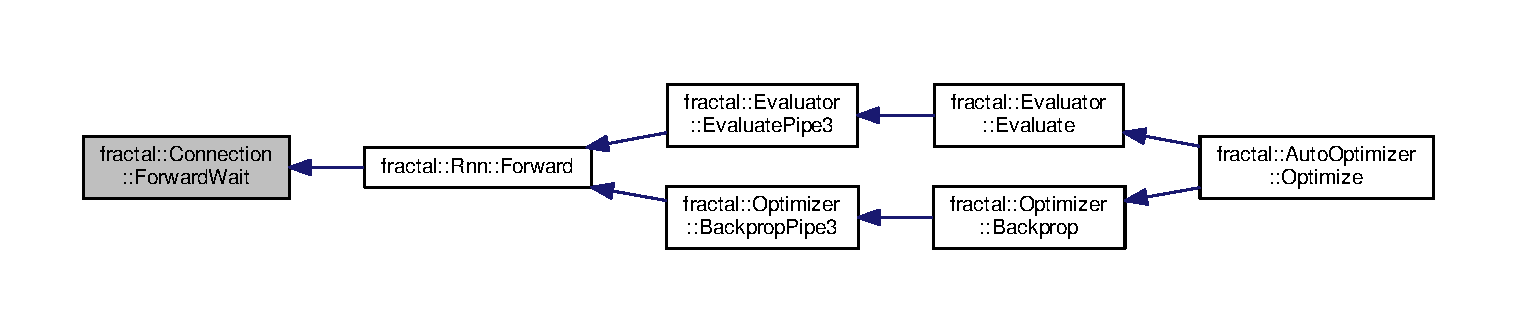
\includegraphics[width=350pt]{da/dbf/classfractal_1_1Connection_a4ccde8145227156ce639a1c050ddb2a4_icgraph}
\end{center}
\end{figure}


\hypertarget{classfractal_1_1Connection_afeb565eb5cf7f0a86d78fb0b111eebc8}{\index{fractal\+::\+Connection@{fractal\+::\+Connection}!Get\+Dst\+Layer@{Get\+Dst\+Layer}}
\index{Get\+Dst\+Layer@{Get\+Dst\+Layer}!fractal\+::\+Connection@{fractal\+::\+Connection}}
\subsubsection[{Get\+Dst\+Layer}]{\setlength{\rightskip}{0pt plus 5cm}{\bf Layer}$\ast$ const fractal\+::\+Connection\+::\+Get\+Dst\+Layer (
\begin{DoxyParamCaption}
{}
\end{DoxyParamCaption}
) const\hspace{0.3cm}{\ttfamily [inline]}}}\label{classfractal_1_1Connection_afeb565eb5cf7f0a86d78fb0b111eebc8}


Definition at line 65 of file Connection.\+h.



Here is the caller graph for this function\+:\nopagebreak
\begin{figure}[H]
\begin{center}
\leavevmode
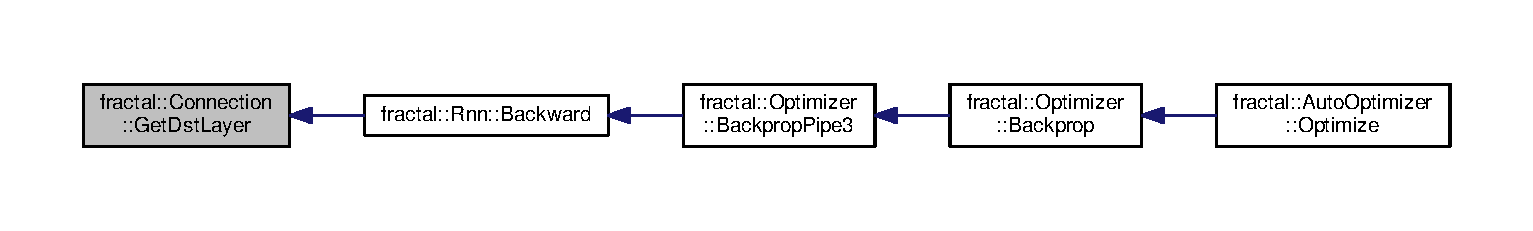
\includegraphics[width=350pt]{da/dbf/classfractal_1_1Connection_afeb565eb5cf7f0a86d78fb0b111eebc8_icgraph}
\end{center}
\end{figure}


\hypertarget{classfractal_1_1Connection_a8da7f0061214ed460eef30d18be2966d}{\index{fractal\+::\+Connection@{fractal\+::\+Connection}!Get\+Num\+Weights@{Get\+Num\+Weights}}
\index{Get\+Num\+Weights@{Get\+Num\+Weights}!fractal\+::\+Connection@{fractal\+::\+Connection}}
\subsubsection[{Get\+Num\+Weights}]{\setlength{\rightskip}{0pt plus 5cm}const unsigned long fractal\+::\+Connection\+::\+Get\+Num\+Weights (
\begin{DoxyParamCaption}
{}
\end{DoxyParamCaption}
)}}\label{classfractal_1_1Connection_a8da7f0061214ed460eef30d18be2966d}


Definition at line 500 of file Connection.\+cc.



Here is the call graph for this function\+:\nopagebreak
\begin{figure}[H]
\begin{center}
\leavevmode
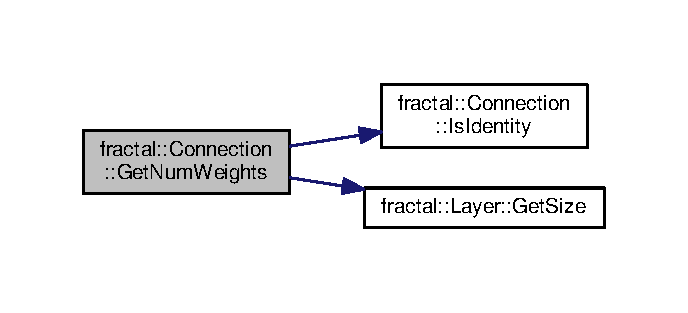
\includegraphics[width=330pt]{da/dbf/classfractal_1_1Connection_a8da7f0061214ed460eef30d18be2966d_cgraph}
\end{center}
\end{figure}


\hypertarget{classfractal_1_1Connection_ad8d0ba5c34c518c24f3104448c5b0d6f}{\index{fractal\+::\+Connection@{fractal\+::\+Connection}!Get\+P\+Stream@{Get\+P\+Stream}}
\index{Get\+P\+Stream@{Get\+P\+Stream}!fractal\+::\+Connection@{fractal\+::\+Connection}}
\subsubsection[{Get\+P\+Stream}]{\setlength{\rightskip}{0pt plus 5cm}{\bf P\+Stream} \& fractal\+::\+Connection\+::\+Get\+P\+Stream (
\begin{DoxyParamCaption}
{}
\end{DoxyParamCaption}
)}}\label{classfractal_1_1Connection_ad8d0ba5c34c518c24f3104448c5b0d6f}


Definition at line 373 of file Connection.\+cc.

\hypertarget{classfractal_1_1Connection_a7ee554da75a227b017217121e9c0d70e}{\index{fractal\+::\+Connection@{fractal\+::\+Connection}!Get\+Src\+Layer@{Get\+Src\+Layer}}
\index{Get\+Src\+Layer@{Get\+Src\+Layer}!fractal\+::\+Connection@{fractal\+::\+Connection}}
\subsubsection[{Get\+Src\+Layer}]{\setlength{\rightskip}{0pt plus 5cm}{\bf Layer}$\ast$ const fractal\+::\+Connection\+::\+Get\+Src\+Layer (
\begin{DoxyParamCaption}
{}
\end{DoxyParamCaption}
) const\hspace{0.3cm}{\ttfamily [inline]}}}\label{classfractal_1_1Connection_a7ee554da75a227b017217121e9c0d70e}


Definition at line 64 of file Connection.\+h.



Here is the caller graph for this function\+:\nopagebreak
\begin{figure}[H]
\begin{center}
\leavevmode
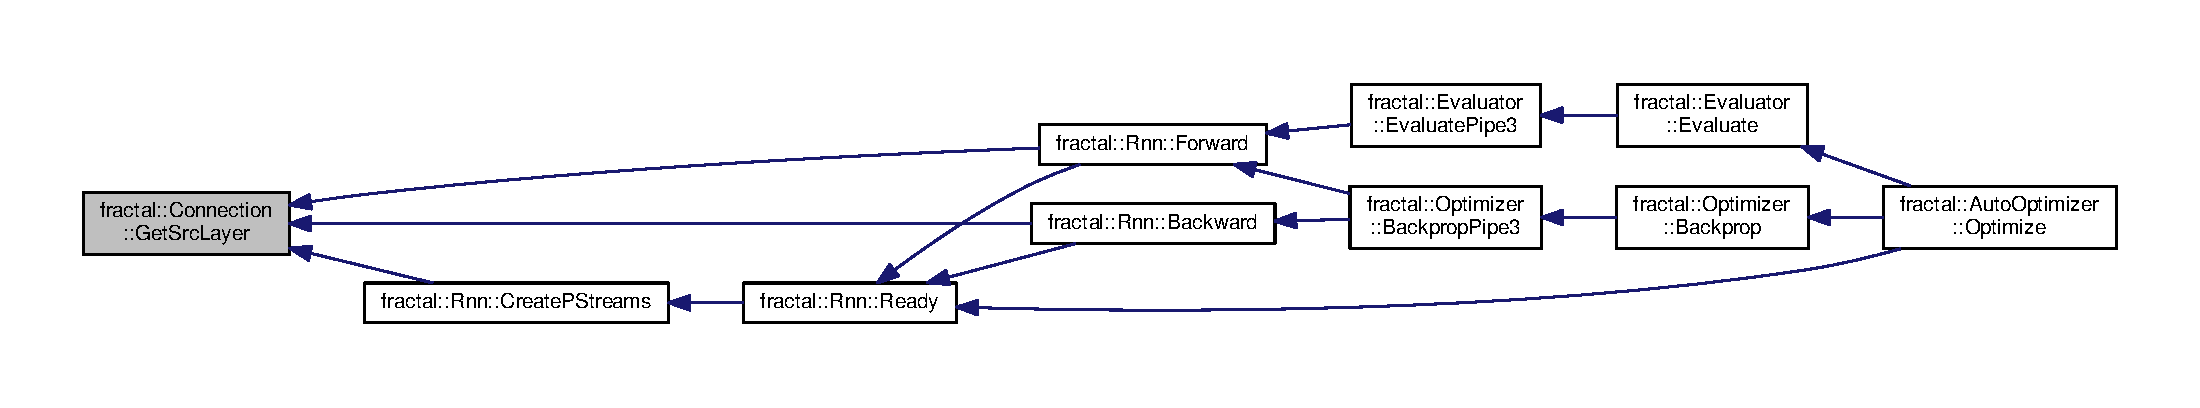
\includegraphics[width=350pt]{da/dbf/classfractal_1_1Connection_a7ee554da75a227b017217121e9c0d70e_icgraph}
\end{center}
\end{figure}


\hypertarget{classfractal_1_1Connection_a6beb3752a66f62f60238c22430486593}{\index{fractal\+::\+Connection@{fractal\+::\+Connection}!Init\+Adadelta@{Init\+Adadelta}}
\index{Init\+Adadelta@{Init\+Adadelta}!fractal\+::\+Connection@{fractal\+::\+Connection}}
\subsubsection[{Init\+Adadelta}]{\setlength{\rightskip}{0pt plus 5cm}void fractal\+::\+Connection\+::\+Init\+Adadelta (
\begin{DoxyParamCaption}
\item[{const {\bf F\+L\+O\+A\+T}}]{decay\+Rate}
\end{DoxyParamCaption}
)}}\label{classfractal_1_1Connection_a6beb3752a66f62f60238c22430486593}


Definition at line 138 of file Connection.\+cc.



Here is the call graph for this function\+:\nopagebreak
\begin{figure}[H]
\begin{center}
\leavevmode
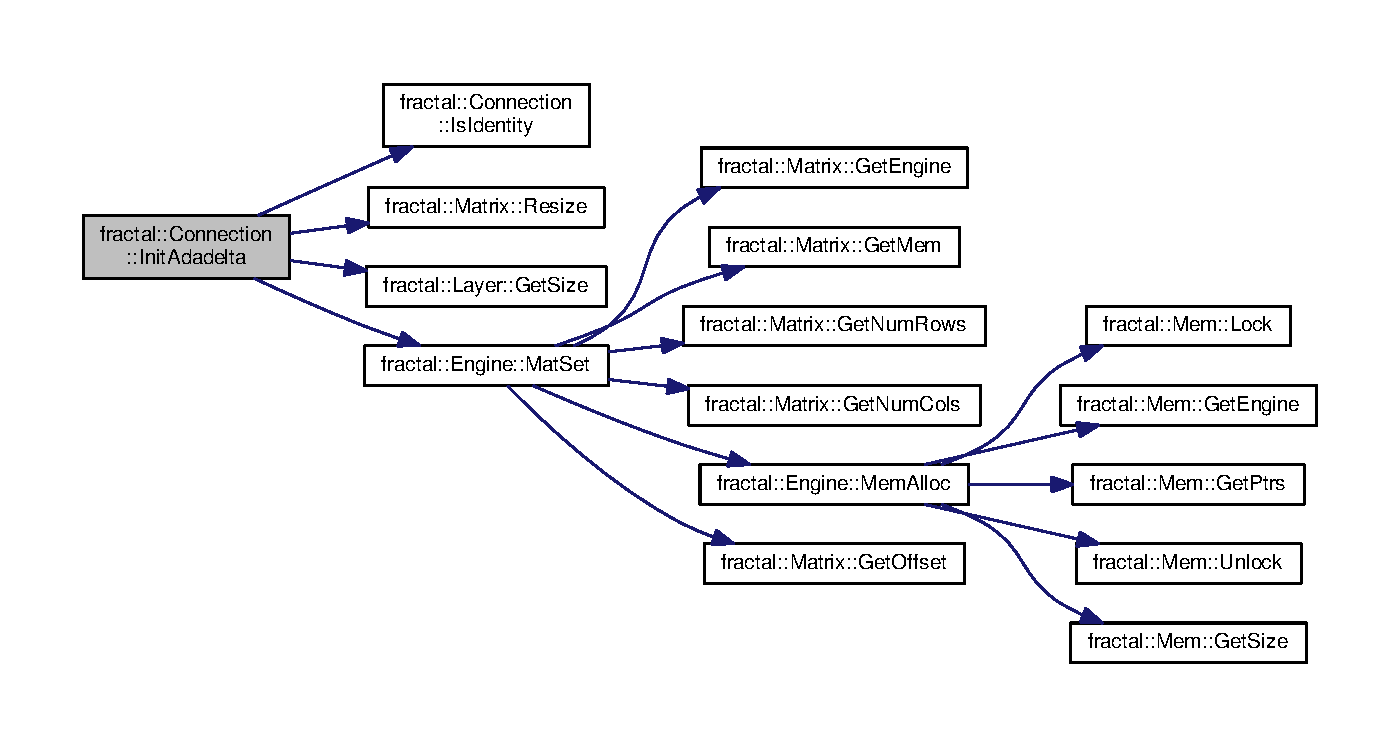
\includegraphics[width=350pt]{da/dbf/classfractal_1_1Connection_a6beb3752a66f62f60238c22430486593_cgraph}
\end{center}
\end{figure}


\hypertarget{classfractal_1_1Connection_a07f221e1751d01ed357b8bd4cc49dfbc}{\index{fractal\+::\+Connection@{fractal\+::\+Connection}!Init\+Err@{Init\+Err}}
\index{Init\+Err@{Init\+Err}!fractal\+::\+Connection@{fractal\+::\+Connection}}
\subsubsection[{Init\+Err}]{\setlength{\rightskip}{0pt plus 5cm}void fractal\+::\+Connection\+::\+Init\+Err (
\begin{DoxyParamCaption}
\item[{const unsigned long}]{batch\+From, }
\item[{const unsigned long}]{batch\+To}
\end{DoxyParamCaption}
)}}\label{classfractal_1_1Connection_a07f221e1751d01ed357b8bd4cc49dfbc}


Definition at line 183 of file Connection.\+cc.



Here is the call graph for this function\+:\nopagebreak
\begin{figure}[H]
\begin{center}
\leavevmode
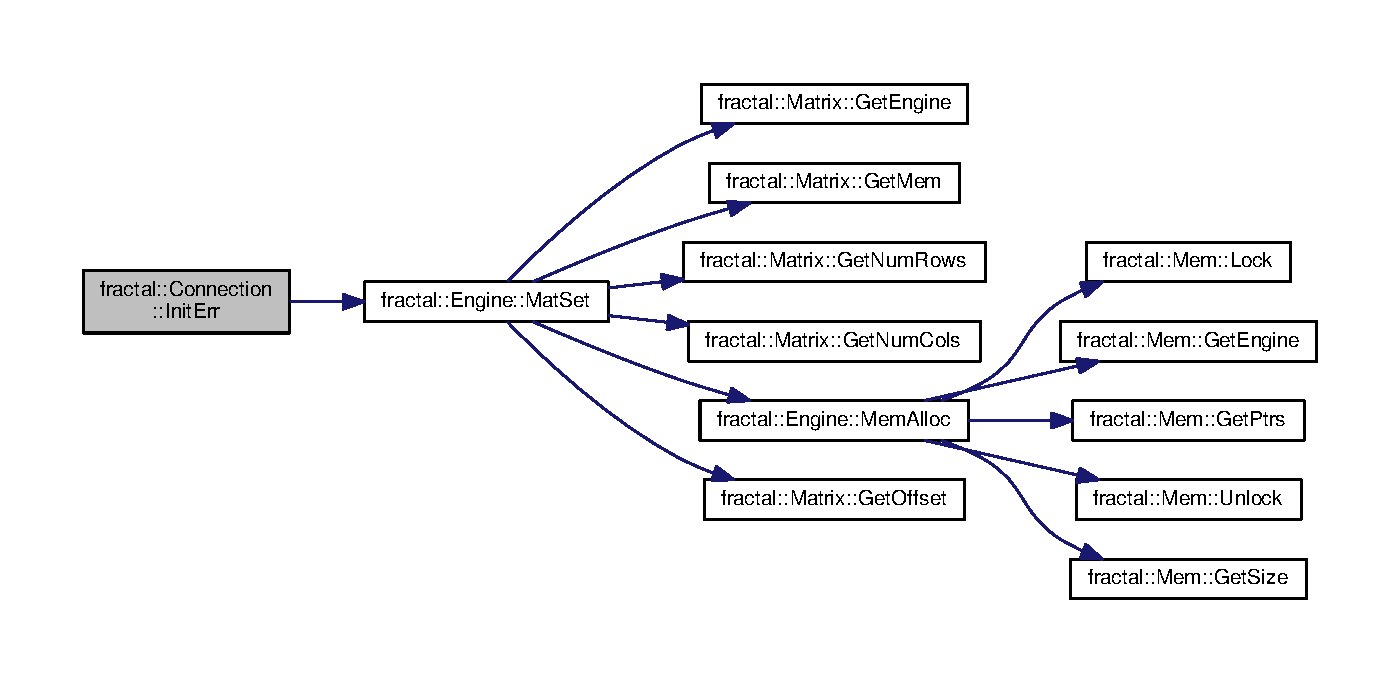
\includegraphics[width=350pt]{da/dbf/classfractal_1_1Connection_a07f221e1751d01ed357b8bd4cc49dfbc_cgraph}
\end{center}
\end{figure}


\hypertarget{classfractal_1_1Connection_addddbba4b7044cad62a0541d26569f3b}{\index{fractal\+::\+Connection@{fractal\+::\+Connection}!Init\+Nesterov@{Init\+Nesterov}}
\index{Init\+Nesterov@{Init\+Nesterov}!fractal\+::\+Connection@{fractal\+::\+Connection}}
\subsubsection[{Init\+Nesterov}]{\setlength{\rightskip}{0pt plus 5cm}void fractal\+::\+Connection\+::\+Init\+Nesterov (
\begin{DoxyParamCaption}
{}
\end{DoxyParamCaption}
)}}\label{classfractal_1_1Connection_addddbba4b7044cad62a0541d26569f3b}


Definition at line 156 of file Connection.\+cc.



Here is the call graph for this function\+:\nopagebreak
\begin{figure}[H]
\begin{center}
\leavevmode
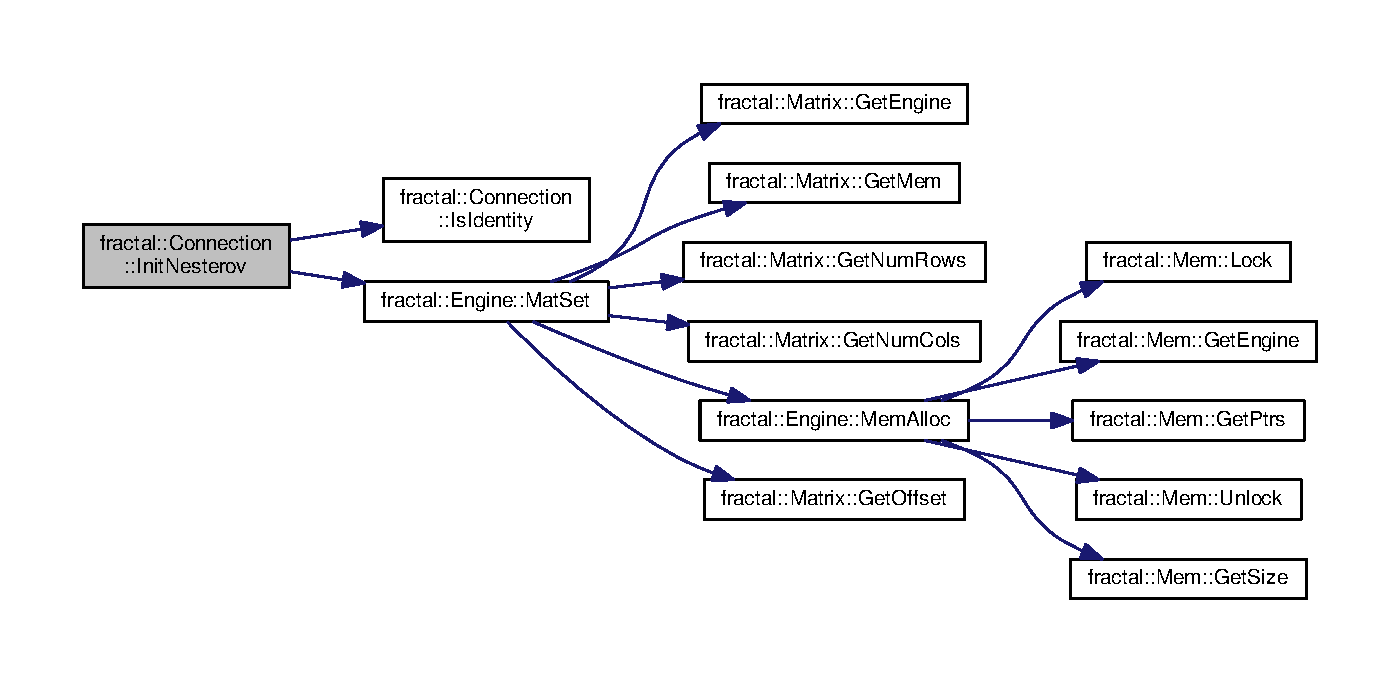
\includegraphics[width=350pt]{da/dbf/classfractal_1_1Connection_addddbba4b7044cad62a0541d26569f3b_cgraph}
\end{center}
\end{figure}


\hypertarget{classfractal_1_1Connection_a74c18a8efe61e4890c69b26063f74175}{\index{fractal\+::\+Connection@{fractal\+::\+Connection}!Init\+Rmsprop@{Init\+Rmsprop}}
\index{Init\+Rmsprop@{Init\+Rmsprop}!fractal\+::\+Connection@{fractal\+::\+Connection}}
\subsubsection[{Init\+Rmsprop}]{\setlength{\rightskip}{0pt plus 5cm}void fractal\+::\+Connection\+::\+Init\+Rmsprop (
\begin{DoxyParamCaption}
\item[{const {\bf F\+L\+O\+A\+T}}]{decay\+Rate}
\end{DoxyParamCaption}
)}}\label{classfractal_1_1Connection_a74c18a8efe61e4890c69b26063f74175}


Definition at line 167 of file Connection.\+cc.



Here is the call graph for this function\+:\nopagebreak
\begin{figure}[H]
\begin{center}
\leavevmode
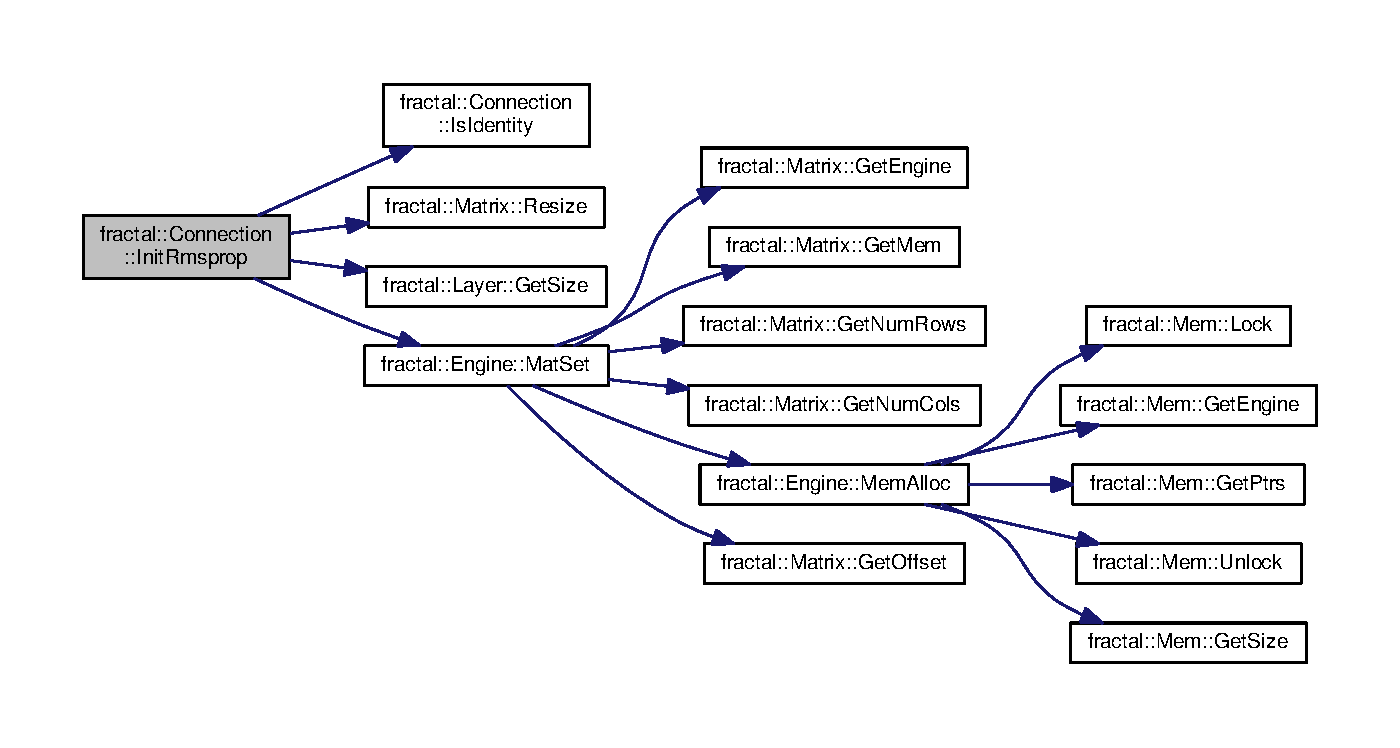
\includegraphics[width=350pt]{da/dbf/classfractal_1_1Connection_a74c18a8efe61e4890c69b26063f74175_cgraph}
\end{center}
\end{figure}


\hypertarget{classfractal_1_1Connection_a462d4925a2c205cf6c1640efe6b723be}{\index{fractal\+::\+Connection@{fractal\+::\+Connection}!Init\+Weights@{Init\+Weights}}
\index{Init\+Weights@{Init\+Weights}!fractal\+::\+Connection@{fractal\+::\+Connection}}
\subsubsection[{Init\+Weights}]{\setlength{\rightskip}{0pt plus 5cm}void fractal\+::\+Connection\+::\+Init\+Weights (
\begin{DoxyParamCaption}
\item[{const {\bf Init\+Weight\+Param} \&}]{param}
\end{DoxyParamCaption}
)}}\label{classfractal_1_1Connection_a462d4925a2c205cf6c1640efe6b723be}


Definition at line 125 of file Connection.\+cc.



Here is the call graph for this function\+:\nopagebreak
\begin{figure}[H]
\begin{center}
\leavevmode
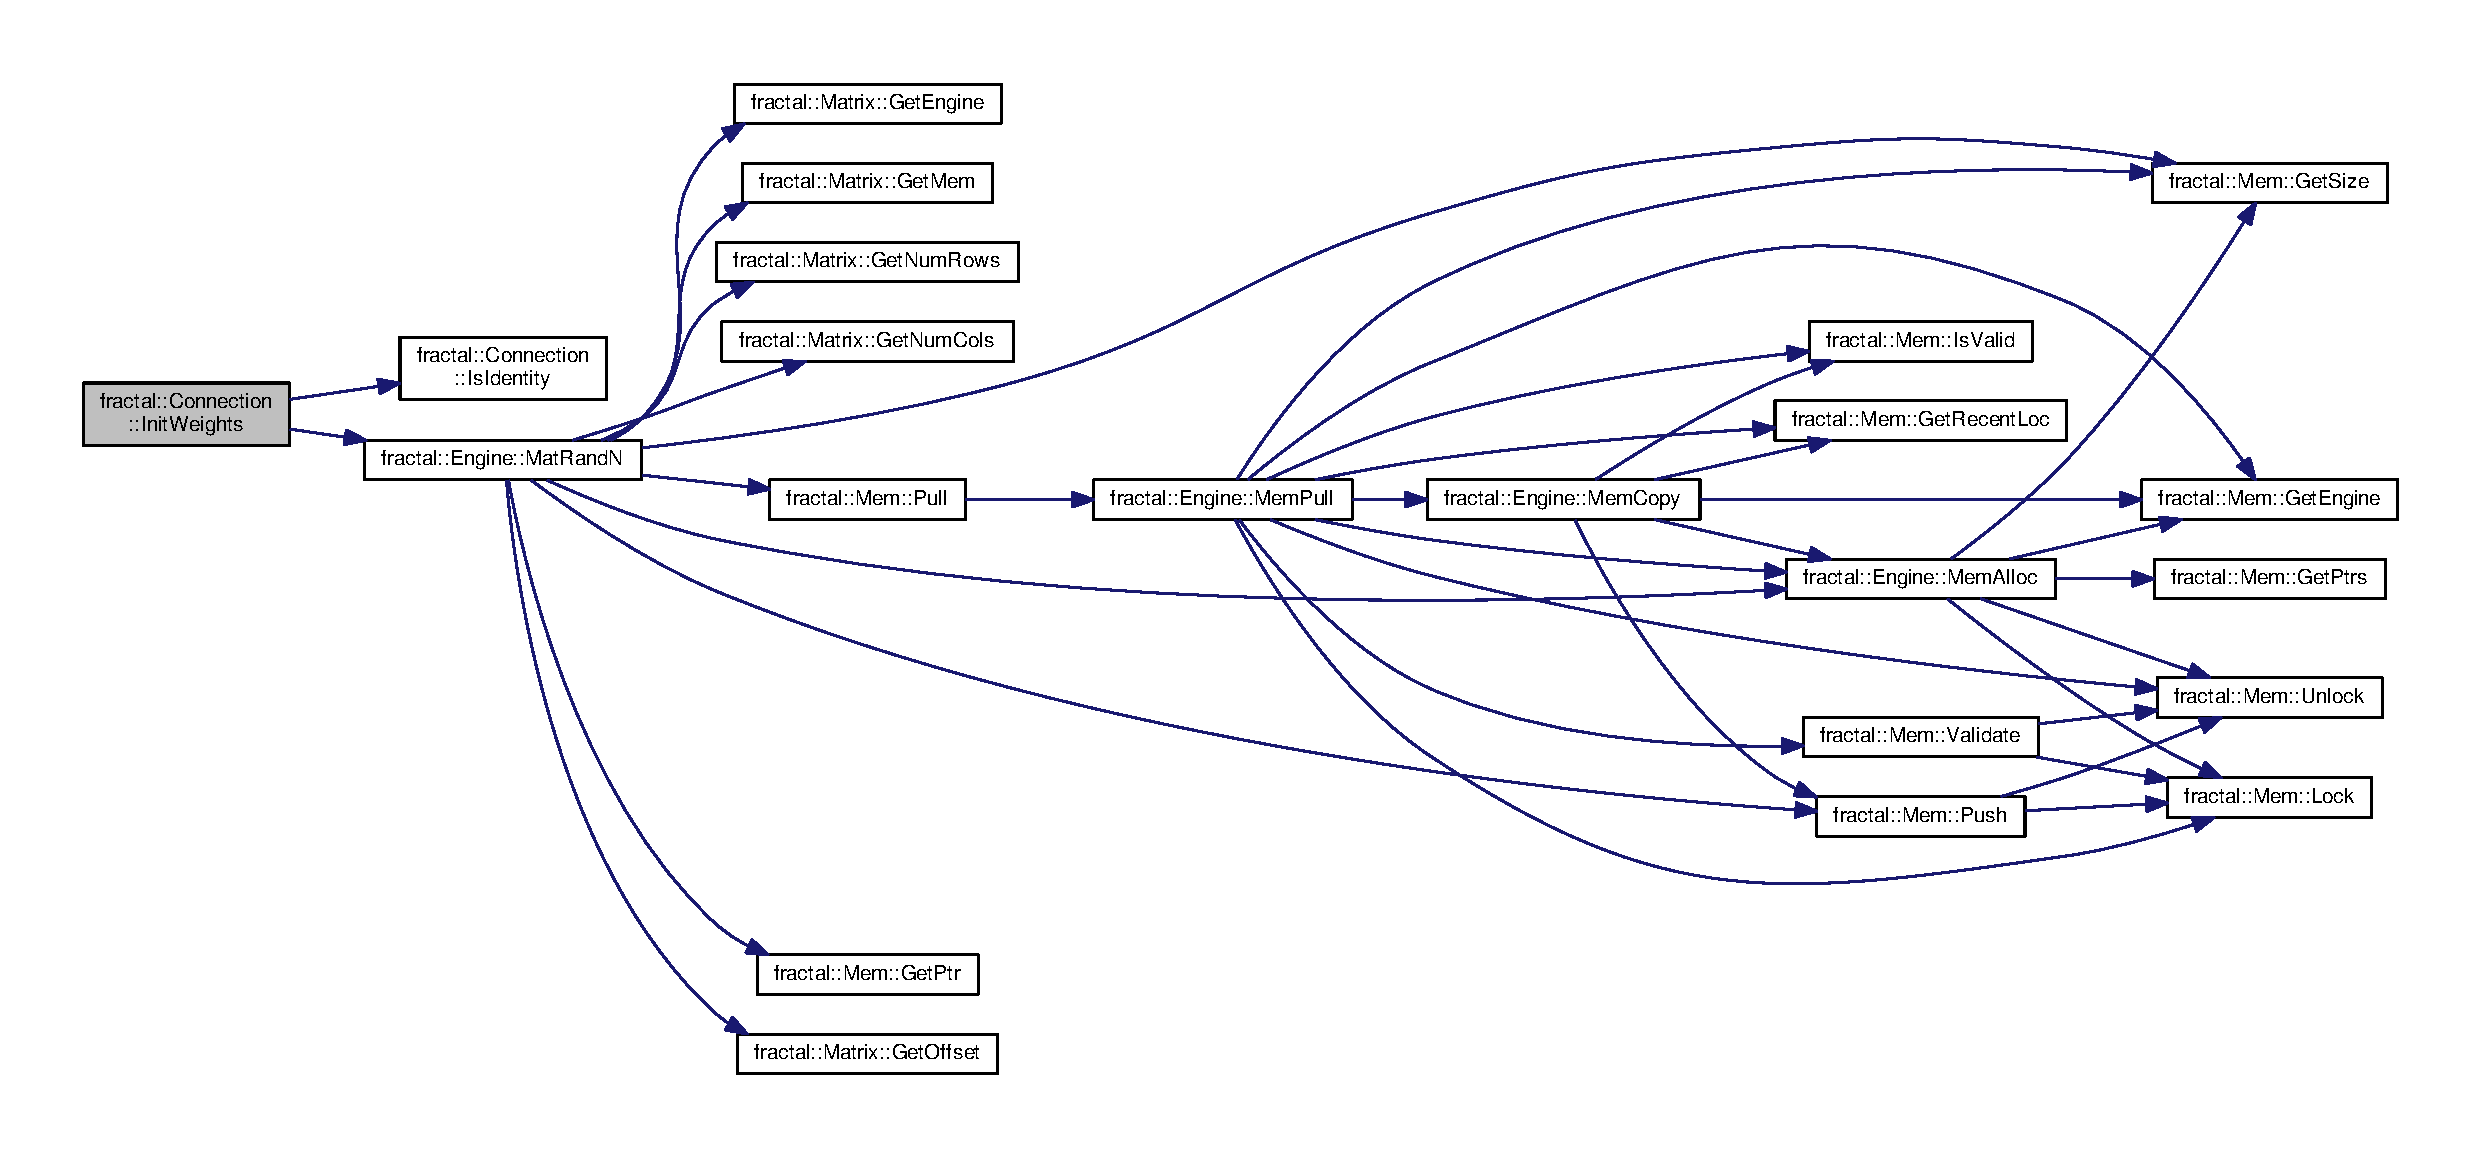
\includegraphics[width=350pt]{da/dbf/classfractal_1_1Connection_a462d4925a2c205cf6c1640efe6b723be_cgraph}
\end{center}
\end{figure}




Here is the caller graph for this function\+:\nopagebreak
\begin{figure}[H]
\begin{center}
\leavevmode
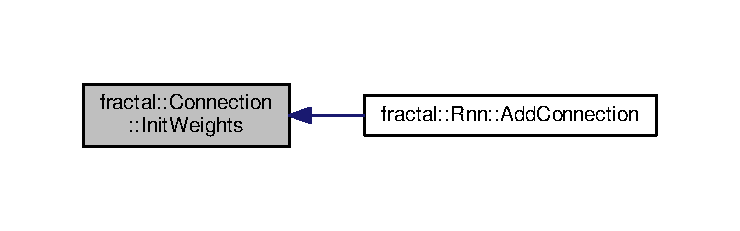
\includegraphics[width=350pt]{da/dbf/classfractal_1_1Connection_a462d4925a2c205cf6c1640efe6b723be_icgraph}
\end{center}
\end{figure}


\hypertarget{classfractal_1_1Connection_a55a98b43749d2af37c492046bdabae30}{\index{fractal\+::\+Connection@{fractal\+::\+Connection}!Is\+Delayed@{Is\+Delayed}}
\index{Is\+Delayed@{Is\+Delayed}!fractal\+::\+Connection@{fractal\+::\+Connection}}
\subsubsection[{Is\+Delayed}]{\setlength{\rightskip}{0pt plus 5cm}const bool fractal\+::\+Connection\+::\+Is\+Delayed (
\begin{DoxyParamCaption}
{}
\end{DoxyParamCaption}
) const\hspace{0.3cm}{\ttfamily [inline]}}}\label{classfractal_1_1Connection_a55a98b43749d2af37c492046bdabae30}


Definition at line 62 of file Connection.\+h.



Here is the caller graph for this function\+:\nopagebreak
\begin{figure}[H]
\begin{center}
\leavevmode
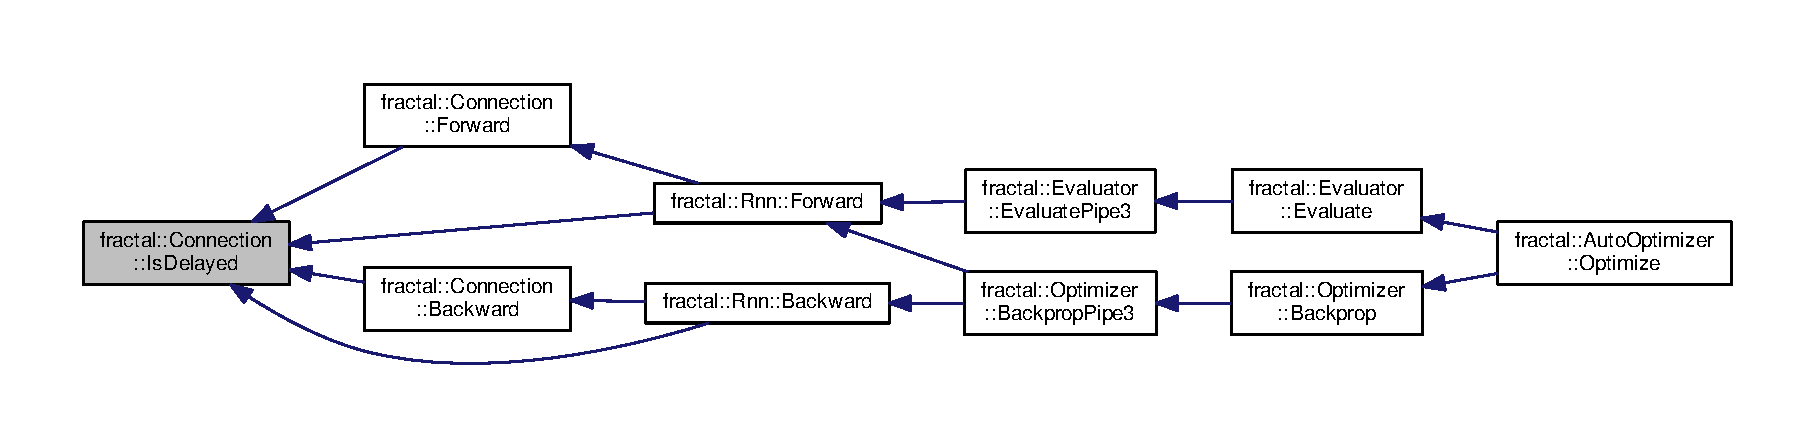
\includegraphics[width=350pt]{da/dbf/classfractal_1_1Connection_a55a98b43749d2af37c492046bdabae30_icgraph}
\end{center}
\end{figure}


\hypertarget{classfractal_1_1Connection_a88b1bd4a69a9c1533ce0d2b261ad0825}{\index{fractal\+::\+Connection@{fractal\+::\+Connection}!Is\+Identity@{Is\+Identity}}
\index{Is\+Identity@{Is\+Identity}!fractal\+::\+Connection@{fractal\+::\+Connection}}
\subsubsection[{Is\+Identity}]{\setlength{\rightskip}{0pt plus 5cm}const bool fractal\+::\+Connection\+::\+Is\+Identity (
\begin{DoxyParamCaption}
{}
\end{DoxyParamCaption}
) const\hspace{0.3cm}{\ttfamily [inline]}}}\label{classfractal_1_1Connection_a88b1bd4a69a9c1533ce0d2b261ad0825}


Definition at line 63 of file Connection.\+h.



Here is the caller graph for this function\+:\nopagebreak
\begin{figure}[H]
\begin{center}
\leavevmode
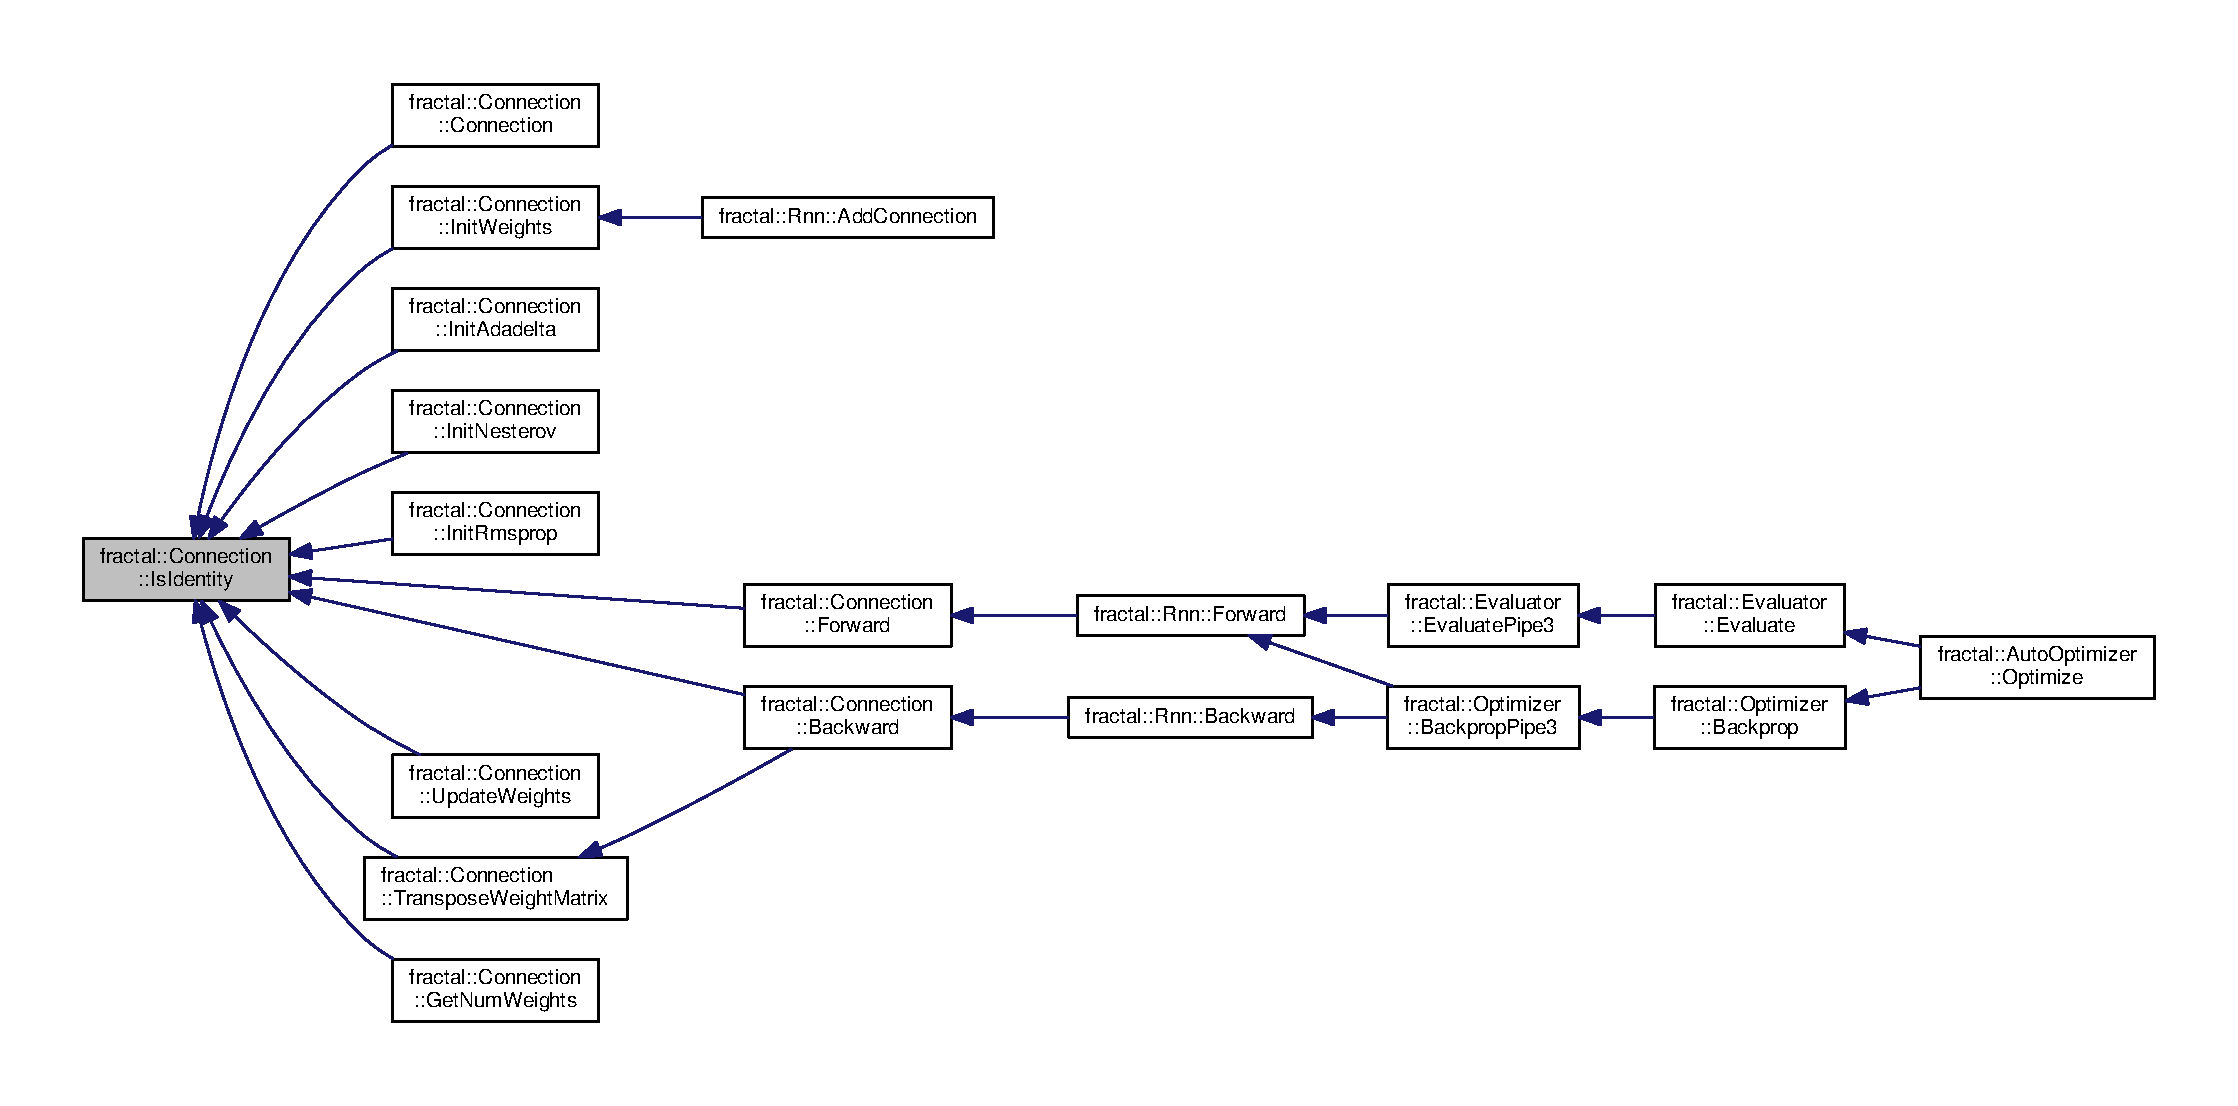
\includegraphics[width=350pt]{da/dbf/classfractal_1_1Connection_a88b1bd4a69a9c1533ce0d2b261ad0825_icgraph}
\end{center}
\end{figure}


\hypertarget{classfractal_1_1Connection_a0539fa32a3eab1298eb7c373114fcc9e}{\index{fractal\+::\+Connection@{fractal\+::\+Connection}!Load\+State@{Load\+State}}
\index{Load\+State@{Load\+State}!fractal\+::\+Connection@{fractal\+::\+Connection}}
\subsubsection[{Load\+State}]{\setlength{\rightskip}{0pt plus 5cm}void fractal\+::\+Connection\+::\+Load\+State (
\begin{DoxyParamCaption}
\item[{const std\+::string \&}]{filename}
\end{DoxyParamCaption}
)}}\label{classfractal_1_1Connection_a0539fa32a3eab1298eb7c373114fcc9e}


Definition at line 446 of file Connection.\+cc.



Here is the call graph for this function\+:\nopagebreak
\begin{figure}[H]
\begin{center}
\leavevmode
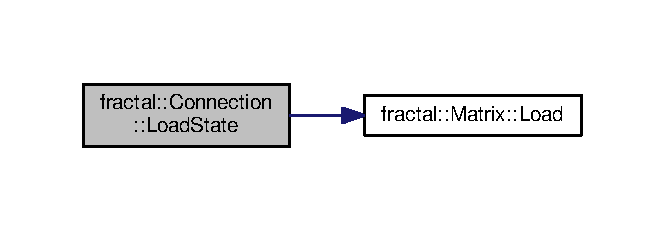
\includegraphics[width=319pt]{da/dbf/classfractal_1_1Connection_a0539fa32a3eab1298eb7c373114fcc9e_cgraph}
\end{center}
\end{figure}


\hypertarget{classfractal_1_1Connection_ae6c82dd4868442e324489ea88d12121d}{\index{fractal\+::\+Connection@{fractal\+::\+Connection}!Save\+State@{Save\+State}}
\index{Save\+State@{Save\+State}!fractal\+::\+Connection@{fractal\+::\+Connection}}
\subsubsection[{Save\+State}]{\setlength{\rightskip}{0pt plus 5cm}void fractal\+::\+Connection\+::\+Save\+State (
\begin{DoxyParamCaption}
\item[{const std\+::string \&}]{filename}
\end{DoxyParamCaption}
)}}\label{classfractal_1_1Connection_ae6c82dd4868442e324489ea88d12121d}


Definition at line 419 of file Connection.\+cc.



Here is the call graph for this function\+:\nopagebreak
\begin{figure}[H]
\begin{center}
\leavevmode
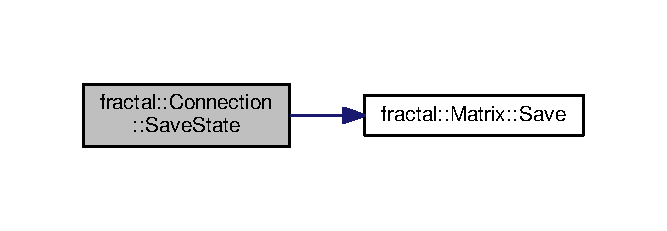
\includegraphics[width=320pt]{da/dbf/classfractal_1_1Connection_ae6c82dd4868442e324489ea88d12121d_cgraph}
\end{center}
\end{figure}


\hypertarget{classfractal_1_1Connection_a09020f3027a886b7971baba901d8bf41}{\index{fractal\+::\+Connection@{fractal\+::\+Connection}!Set\+Batch\+Size@{Set\+Batch\+Size}}
\index{Set\+Batch\+Size@{Set\+Batch\+Size}!fractal\+::\+Connection@{fractal\+::\+Connection}}
\subsubsection[{Set\+Batch\+Size}]{\setlength{\rightskip}{0pt plus 5cm}void fractal\+::\+Connection\+::\+Set\+Batch\+Size (
\begin{DoxyParamCaption}
\item[{const unsigned long}]{batch\+Size}
\end{DoxyParamCaption}
)}}\label{classfractal_1_1Connection_a09020f3027a886b7971baba901d8bf41}


Definition at line 93 of file Connection.\+cc.



Here is the call graph for this function\+:\nopagebreak
\begin{figure}[H]
\begin{center}
\leavevmode
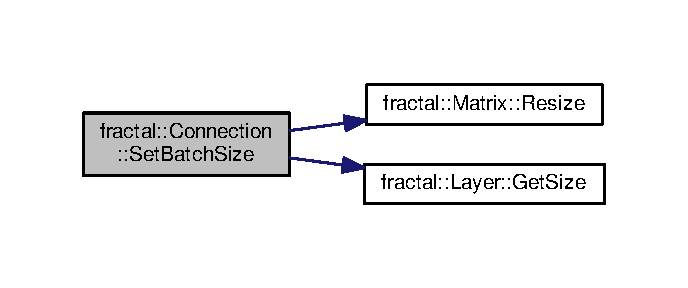
\includegraphics[width=330pt]{da/dbf/classfractal_1_1Connection_a09020f3027a886b7971baba901d8bf41_cgraph}
\end{center}
\end{figure}




Here is the caller graph for this function\+:\nopagebreak
\begin{figure}[H]
\begin{center}
\leavevmode
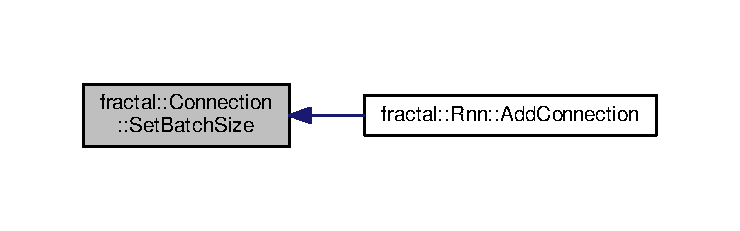
\includegraphics[width=350pt]{da/dbf/classfractal_1_1Connection_a09020f3027a886b7971baba901d8bf41_icgraph}
\end{center}
\end{figure}


\hypertarget{classfractal_1_1Connection_a923b6313b13f60a464d417e638c4382b}{\index{fractal\+::\+Connection@{fractal\+::\+Connection}!Set\+Engine@{Set\+Engine}}
\index{Set\+Engine@{Set\+Engine}!fractal\+::\+Connection@{fractal\+::\+Connection}}
\subsubsection[{Set\+Engine}]{\setlength{\rightskip}{0pt plus 5cm}void fractal\+::\+Connection\+::\+Set\+Engine (
\begin{DoxyParamCaption}
\item[{{\bf Engine} $\ast$const}]{engine, }
\item[{{\bf P\+Stream} $\ast$const}]{stream}
\end{DoxyParamCaption}
)}}\label{classfractal_1_1Connection_a923b6313b13f60a464d417e638c4382b}


Definition at line 60 of file Connection.\+cc.



Here is the call graph for this function\+:\nopagebreak
\begin{figure}[H]
\begin{center}
\leavevmode
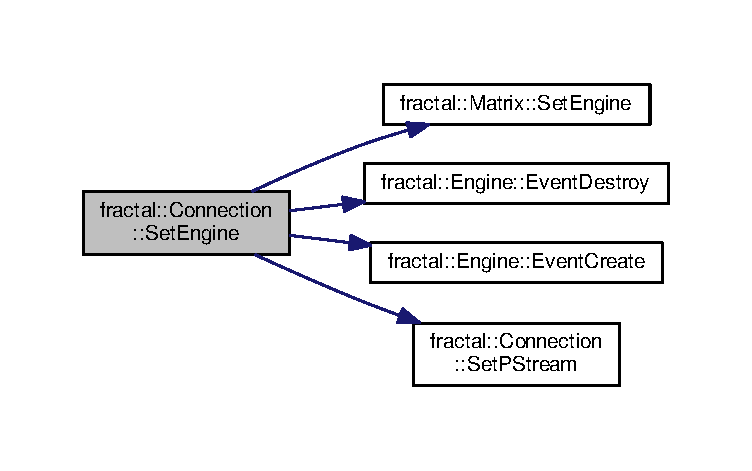
\includegraphics[width=350pt]{da/dbf/classfractal_1_1Connection_a923b6313b13f60a464d417e638c4382b_cgraph}
\end{center}
\end{figure}




Here is the caller graph for this function\+:\nopagebreak
\begin{figure}[H]
\begin{center}
\leavevmode
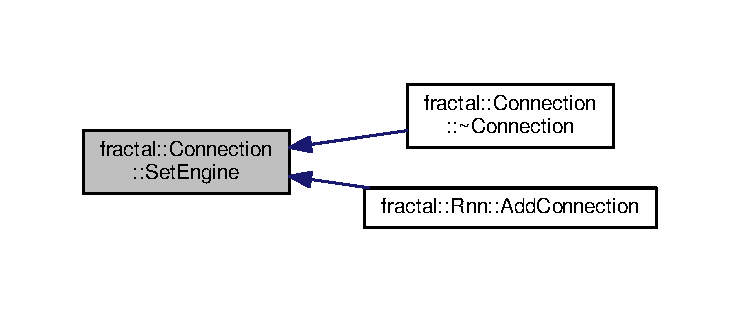
\includegraphics[width=350pt]{da/dbf/classfractal_1_1Connection_a923b6313b13f60a464d417e638c4382b_icgraph}
\end{center}
\end{figure}


\hypertarget{classfractal_1_1Connection_adf2811ab3189c8e4733b157486b26eb6}{\index{fractal\+::\+Connection@{fractal\+::\+Connection}!Set\+P\+Stream@{Set\+P\+Stream}}
\index{Set\+P\+Stream@{Set\+P\+Stream}!fractal\+::\+Connection@{fractal\+::\+Connection}}
\subsubsection[{Set\+P\+Stream}]{\setlength{\rightskip}{0pt plus 5cm}void fractal\+::\+Connection\+::\+Set\+P\+Stream (
\begin{DoxyParamCaption}
\item[{{\bf P\+Stream} $\ast$const}]{stream}
\end{DoxyParamCaption}
)}}\label{classfractal_1_1Connection_adf2811ab3189c8e4733b157486b26eb6}


Definition at line 366 of file Connection.\+cc.



Here is the caller graph for this function\+:\nopagebreak
\begin{figure}[H]
\begin{center}
\leavevmode
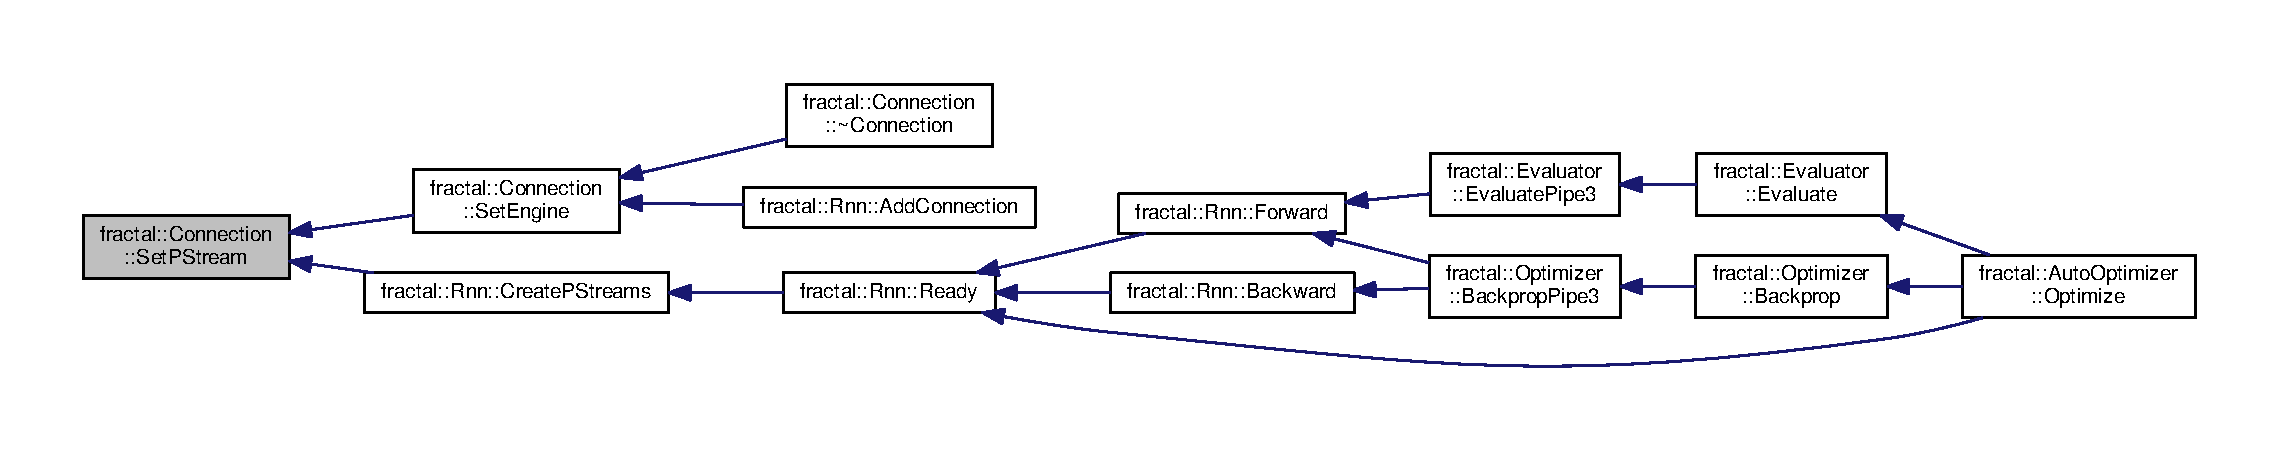
\includegraphics[width=350pt]{da/dbf/classfractal_1_1Connection_adf2811ab3189c8e4733b157486b26eb6_icgraph}
\end{center}
\end{figure}


\hypertarget{classfractal_1_1Connection_a74c50d78f6c779d0a82a58f097fca3ef}{\index{fractal\+::\+Connection@{fractal\+::\+Connection}!Stream\+Wait\+Event@{Stream\+Wait\+Event}}
\index{Stream\+Wait\+Event@{Stream\+Wait\+Event}!fractal\+::\+Connection@{fractal\+::\+Connection}}
\subsubsection[{Stream\+Wait\+Event}]{\setlength{\rightskip}{0pt plus 5cm}void fractal\+::\+Connection\+::\+Stream\+Wait\+Event (
\begin{DoxyParamCaption}
\item[{{\bf P\+Stream} \&}]{stream}
\end{DoxyParamCaption}
)}}\label{classfractal_1_1Connection_a74c50d78f6c779d0a82a58f097fca3ef}


Definition at line 387 of file Connection.\+cc.



Here is the call graph for this function\+:\nopagebreak
\begin{figure}[H]
\begin{center}
\leavevmode
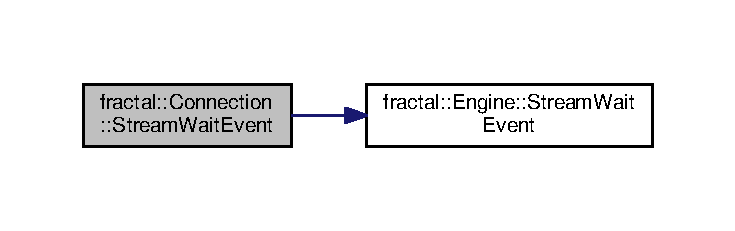
\includegraphics[width=350pt]{da/dbf/classfractal_1_1Connection_a74c50d78f6c779d0a82a58f097fca3ef_cgraph}
\end{center}
\end{figure}


\hypertarget{classfractal_1_1Connection_a9901894e4bd46fdcc7a8d8aa8c35b586}{\index{fractal\+::\+Connection@{fractal\+::\+Connection}!Transpose\+Weight\+Matrix@{Transpose\+Weight\+Matrix}}
\index{Transpose\+Weight\+Matrix@{Transpose\+Weight\+Matrix}!fractal\+::\+Connection@{fractal\+::\+Connection}}
\subsubsection[{Transpose\+Weight\+Matrix}]{\setlength{\rightskip}{0pt plus 5cm}void fractal\+::\+Connection\+::\+Transpose\+Weight\+Matrix (
\begin{DoxyParamCaption}
{}
\end{DoxyParamCaption}
)\hspace{0.3cm}{\ttfamily [protected]}}}\label{classfractal_1_1Connection_a9901894e4bd46fdcc7a8d8aa8c35b586}


Definition at line 406 of file Connection.\+cc.



Here is the call graph for this function\+:\nopagebreak
\begin{figure}[H]
\begin{center}
\leavevmode
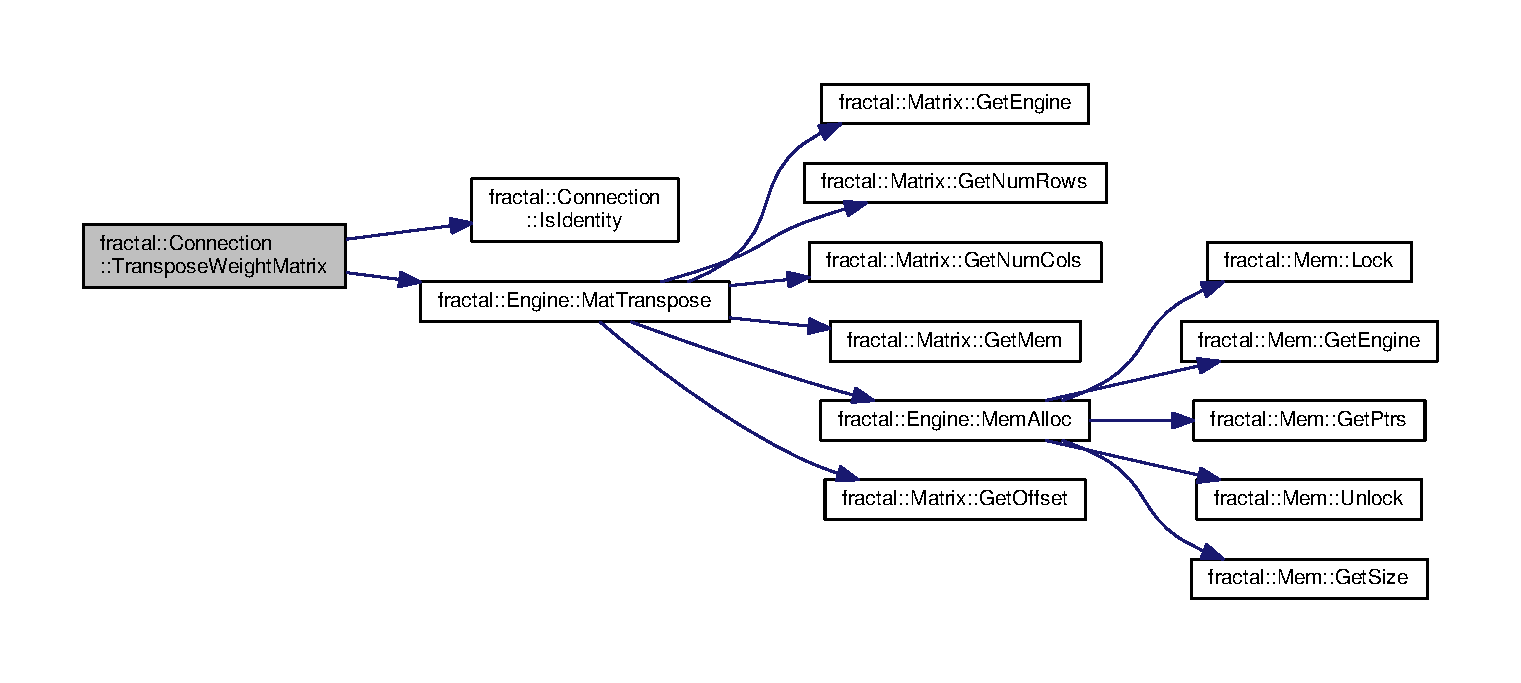
\includegraphics[width=350pt]{da/dbf/classfractal_1_1Connection_a9901894e4bd46fdcc7a8d8aa8c35b586_cgraph}
\end{center}
\end{figure}




Here is the caller graph for this function\+:\nopagebreak
\begin{figure}[H]
\begin{center}
\leavevmode
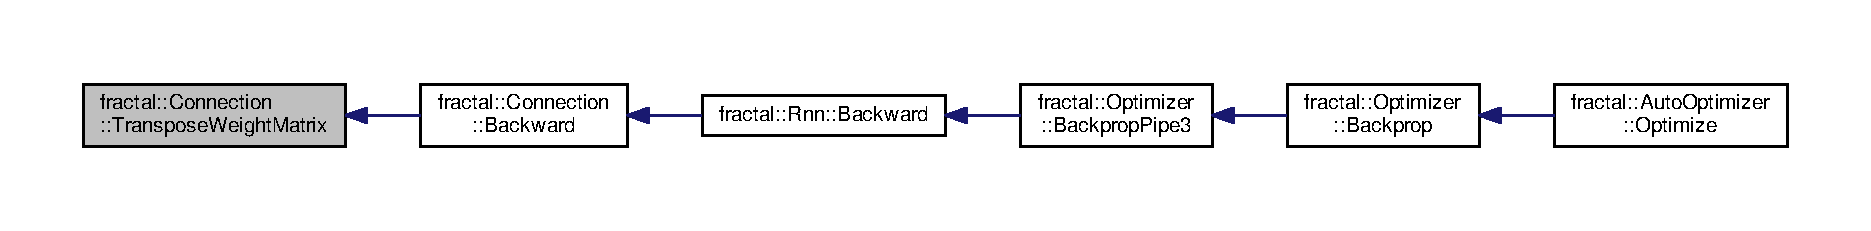
\includegraphics[width=350pt]{da/dbf/classfractal_1_1Connection_a9901894e4bd46fdcc7a8d8aa8c35b586_icgraph}
\end{center}
\end{figure}


\hypertarget{classfractal_1_1Connection_aab6dbd77374b404539f59d26d6c8f798}{\index{fractal\+::\+Connection@{fractal\+::\+Connection}!Unlink\+Matrices@{Unlink\+Matrices}}
\index{Unlink\+Matrices@{Unlink\+Matrices}!fractal\+::\+Connection@{fractal\+::\+Connection}}
\subsubsection[{Unlink\+Matrices}]{\setlength{\rightskip}{0pt plus 5cm}void fractal\+::\+Connection\+::\+Unlink\+Matrices (
\begin{DoxyParamCaption}
{}
\end{DoxyParamCaption}
)}}\label{classfractal_1_1Connection_aab6dbd77374b404539f59d26d6c8f798}


Definition at line 108 of file Connection.\+cc.



Here is the call graph for this function\+:\nopagebreak
\begin{figure}[H]
\begin{center}
\leavevmode
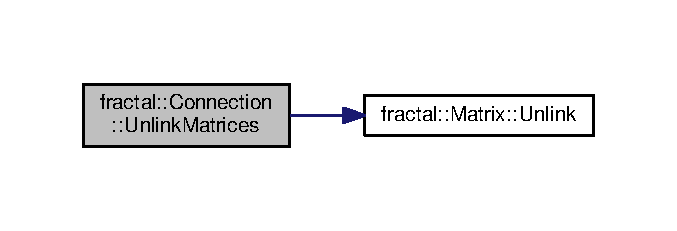
\includegraphics[width=325pt]{da/dbf/classfractal_1_1Connection_aab6dbd77374b404539f59d26d6c8f798_cgraph}
\end{center}
\end{figure}


\hypertarget{classfractal_1_1Connection_af4754297e3aa7fcf27d68e7fc034d069}{\index{fractal\+::\+Connection@{fractal\+::\+Connection}!Update\+Dst\+Err@{Update\+Dst\+Err}}
\index{Update\+Dst\+Err@{Update\+Dst\+Err}!fractal\+::\+Connection@{fractal\+::\+Connection}}
\subsubsection[{Update\+Dst\+Err}]{\setlength{\rightskip}{0pt plus 5cm}void fractal\+::\+Connection\+::\+Update\+Dst\+Err (
\begin{DoxyParamCaption}
\item[{const unsigned long}]{batch\+From, }
\item[{const unsigned long}]{batch\+To}
\end{DoxyParamCaption}
)}}\label{classfractal_1_1Connection_af4754297e3aa7fcf27d68e7fc034d069}


Definition at line 248 of file Connection.\+cc.



Here is the call graph for this function\+:\nopagebreak
\begin{figure}[H]
\begin{center}
\leavevmode
\includegraphics[width=350pt]{da/dbf/classfractal_1_1Connection_af4754297e3aa7fcf27d68e7fc034d069_cgraph}
\end{center}
\end{figure}




Here is the caller graph for this function\+:\nopagebreak
\begin{figure}[H]
\begin{center}
\leavevmode
\includegraphics[width=350pt]{da/dbf/classfractal_1_1Connection_af4754297e3aa7fcf27d68e7fc034d069_icgraph}
\end{center}
\end{figure}


\hypertarget{classfractal_1_1Connection_a2b8a12fcdb97fe575d48348ac3e42daa}{\index{fractal\+::\+Connection@{fractal\+::\+Connection}!Update\+Weights@{Update\+Weights}}
\index{Update\+Weights@{Update\+Weights}!fractal\+::\+Connection@{fractal\+::\+Connection}}
\subsubsection[{Update\+Weights}]{\setlength{\rightskip}{0pt plus 5cm}void fractal\+::\+Connection\+::\+Update\+Weights (
\begin{DoxyParamCaption}
\item[{const unsigned long}]{batch\+From, }
\item[{const unsigned long}]{batch\+To, }
\item[{const unsigned long}]{n\+Frame, }
\item[{const {\bf F\+L\+O\+A\+T}}]{rate, }
\item[{const {\bf F\+L\+O\+A\+T}}]{momentum, }
\item[{const bool}]{adaptive\+Rates, }
\item[{const bool}]{rmsprop}
\end{DoxyParamCaption}
)}}\label{classfractal_1_1Connection_a2b8a12fcdb97fe575d48348ac3e42daa}


Definition at line 316 of file Connection.\+cc.



Here is the call graph for this function\+:\nopagebreak
\begin{figure}[H]
\begin{center}
\leavevmode
\includegraphics[width=350pt]{da/dbf/classfractal_1_1Connection_a2b8a12fcdb97fe575d48348ac3e42daa_cgraph}
\end{center}
\end{figure}




\subsection{Member Data Documentation}
\hypertarget{classfractal_1_1Connection_aabe650cd29a9133e18de1a99bafd2069}{\index{fractal\+::\+Connection@{fractal\+::\+Connection}!\+\_\+identity@{\+\_\+identity}}
\index{\+\_\+identity@{\+\_\+identity}!fractal\+::\+Connection@{fractal\+::\+Connection}}
\subsubsection[{\+\_\+identity}]{\setlength{\rightskip}{0pt plus 5cm}bool fractal\+::\+Connection\+::\+\_\+identity\hspace{0.3cm}{\ttfamily [protected]}}}\label{classfractal_1_1Connection_aabe650cd29a9133e18de1a99bafd2069}


Definition at line 86 of file Connection.\+h.

\hypertarget{classfractal_1_1Connection_a1c06df140701c272107c47b4ce40792b}{\index{fractal\+::\+Connection@{fractal\+::\+Connection}!batch\+Size@{batch\+Size}}
\index{batch\+Size@{batch\+Size}!fractal\+::\+Connection@{fractal\+::\+Connection}}
\subsubsection[{batch\+Size}]{\setlength{\rightskip}{0pt plus 5cm}unsigned long fractal\+::\+Connection\+::batch\+Size\hspace{0.3cm}{\ttfamily [protected]}}}\label{classfractal_1_1Connection_a1c06df140701c272107c47b4ce40792b}


Definition at line 91 of file Connection.\+h.

\hypertarget{classfractal_1_1Connection_aeed56c0faa379d9c695e49457b63bc03}{\index{fractal\+::\+Connection@{fractal\+::\+Connection}!delay\+Amount@{delay\+Amount}}
\index{delay\+Amount@{delay\+Amount}!fractal\+::\+Connection@{fractal\+::\+Connection}}
\subsubsection[{delay\+Amount}]{\setlength{\rightskip}{0pt plus 5cm}unsigned long fractal\+::\+Connection\+::delay\+Amount\hspace{0.3cm}{\ttfamily [protected]}}}\label{classfractal_1_1Connection_aeed56c0faa379d9c695e49457b63bc03}


Definition at line 87 of file Connection.\+h.

\hypertarget{classfractal_1_1Connection_a31f6cf9d89d0c4166dc8bde044fafd00}{\index{fractal\+::\+Connection@{fractal\+::\+Connection}!derivs@{derivs}}
\index{derivs@{derivs}!fractal\+::\+Connection@{fractal\+::\+Connection}}
\subsubsection[{derivs}]{\setlength{\rightskip}{0pt plus 5cm}{\bf Matrix}$<${\bf F\+L\+O\+A\+T}$>$ fractal\+::\+Connection\+::derivs\hspace{0.3cm}{\ttfamily [protected]}}}\label{classfractal_1_1Connection_a31f6cf9d89d0c4166dc8bde044fafd00}


Definition at line 99 of file Connection.\+h.

\hypertarget{classfractal_1_1Connection_a7e99d505ee81e3c7c00dceb70efdf8bf}{\index{fractal\+::\+Connection@{fractal\+::\+Connection}!dst\+Act@{dst\+Act}}
\index{dst\+Act@{dst\+Act}!fractal\+::\+Connection@{fractal\+::\+Connection}}
\subsubsection[{dst\+Act}]{\setlength{\rightskip}{0pt plus 5cm}{\bf Matrix}$<${\bf F\+L\+O\+A\+T}$>$ fractal\+::\+Connection\+::dst\+Act\hspace{0.3cm}{\ttfamily [protected]}}}\label{classfractal_1_1Connection_a7e99d505ee81e3c7c00dceb70efdf8bf}


Definition at line 101 of file Connection.\+h.

\hypertarget{classfractal_1_1Connection_a2374b05f600966a36a1eec9b0946328d}{\index{fractal\+::\+Connection@{fractal\+::\+Connection}!dst\+Err@{dst\+Err}}
\index{dst\+Err@{dst\+Err}!fractal\+::\+Connection@{fractal\+::\+Connection}}
\subsubsection[{dst\+Err}]{\setlength{\rightskip}{0pt plus 5cm}{\bf Matrix}$<${\bf F\+L\+O\+A\+T}$>$ fractal\+::\+Connection\+::dst\+Err\hspace{0.3cm}{\ttfamily [protected]}}}\label{classfractal_1_1Connection_a2374b05f600966a36a1eec9b0946328d}


Definition at line 102 of file Connection.\+h.

\hypertarget{classfractal_1_1Connection_a43d6bb6d604142602b3e339bb77bda33}{\index{fractal\+::\+Connection@{fractal\+::\+Connection}!dst\+Layer@{dst\+Layer}}
\index{dst\+Layer@{dst\+Layer}!fractal\+::\+Connection@{fractal\+::\+Connection}}
\subsubsection[{dst\+Layer}]{\setlength{\rightskip}{0pt plus 5cm}{\bf Layer} $\ast$ fractal\+::\+Connection\+::dst\+Layer\hspace{0.3cm}{\ttfamily [protected]}}}\label{classfractal_1_1Connection_a43d6bb6d604142602b3e339bb77bda33}


Definition at line 89 of file Connection.\+h.

\hypertarget{classfractal_1_1Connection_aed0a390a46ba6bcdff5c6238ac5b9bda}{\index{fractal\+::\+Connection@{fractal\+::\+Connection}!engine@{engine}}
\index{engine@{engine}!fractal\+::\+Connection@{fractal\+::\+Connection}}
\subsubsection[{engine}]{\setlength{\rightskip}{0pt plus 5cm}{\bf Engine}$\ast$ fractal\+::\+Connection\+::engine\hspace{0.3cm}{\ttfamily [protected]}}}\label{classfractal_1_1Connection_aed0a390a46ba6bcdff5c6238ac5b9bda}


Definition at line 84 of file Connection.\+h.

\hypertarget{classfractal_1_1Connection_a1440177a726771823d046340f1c24e59}{\index{fractal\+::\+Connection@{fractal\+::\+Connection}!event@{event}}
\index{event@{event}!fractal\+::\+Connection@{fractal\+::\+Connection}}
\subsubsection[{event}]{\setlength{\rightskip}{0pt plus 5cm}{\bf P\+Event} fractal\+::\+Connection\+::event\hspace{0.3cm}{\ttfamily [protected]}}}\label{classfractal_1_1Connection_a1440177a726771823d046340f1c24e59}


Definition at line 105 of file Connection.\+h.

\hypertarget{classfractal_1_1Connection_aee958063517851c72a62c55f049300be}{\index{fractal\+::\+Connection@{fractal\+::\+Connection}!Layer@{Layer}}
\index{Layer@{Layer}!fractal\+::\+Connection@{fractal\+::\+Connection}}
\subsubsection[{Layer}]{\setlength{\rightskip}{0pt plus 5cm}friend fractal\+::\+Connection\+::\+Layer\hspace{0.3cm}{\ttfamily [protected]}}}\label{classfractal_1_1Connection_aee958063517851c72a62c55f049300be}


Definition at line 107 of file Connection.\+h.

\hypertarget{classfractal_1_1Connection_a0cd41b30d1dc0db0a6722521a20906ea}{\index{fractal\+::\+Connection@{fractal\+::\+Connection}!ms\+Delta@{ms\+Delta}}
\index{ms\+Delta@{ms\+Delta}!fractal\+::\+Connection@{fractal\+::\+Connection}}
\subsubsection[{ms\+Delta}]{\setlength{\rightskip}{0pt plus 5cm}{\bf Matrix}$<${\bf F\+L\+O\+A\+T}$>$ fractal\+::\+Connection\+::ms\+Delta\hspace{0.3cm}{\ttfamily [protected]}}}\label{classfractal_1_1Connection_a0cd41b30d1dc0db0a6722521a20906ea}


Definition at line 100 of file Connection.\+h.

\hypertarget{classfractal_1_1Connection_ac4df1add96950e005f005047f25f158d}{\index{fractal\+::\+Connection@{fractal\+::\+Connection}!ms\+Deriv@{ms\+Deriv}}
\index{ms\+Deriv@{ms\+Deriv}!fractal\+::\+Connection@{fractal\+::\+Connection}}
\subsubsection[{ms\+Deriv}]{\setlength{\rightskip}{0pt plus 5cm}{\bf Matrix}$<${\bf F\+L\+O\+A\+T}$>$ fractal\+::\+Connection\+::ms\+Deriv\hspace{0.3cm}{\ttfamily [protected]}}}\label{classfractal_1_1Connection_ac4df1add96950e005f005047f25f158d}


Definition at line 99 of file Connection.\+h.

\hypertarget{classfractal_1_1Connection_ade0067c963f876032c92cd4198deaa32}{\index{fractal\+::\+Connection@{fractal\+::\+Connection}!rms\+Decay\+Rate@{rms\+Decay\+Rate}}
\index{rms\+Decay\+Rate@{rms\+Decay\+Rate}!fractal\+::\+Connection@{fractal\+::\+Connection}}
\subsubsection[{rms\+Decay\+Rate}]{\setlength{\rightskip}{0pt plus 5cm}{\bf F\+L\+O\+A\+T} fractal\+::\+Connection\+::rms\+Decay\+Rate\hspace{0.3cm}{\ttfamily [protected]}}}\label{classfractal_1_1Connection_ade0067c963f876032c92cd4198deaa32}


Definition at line 93 of file Connection.\+h.

\hypertarget{classfractal_1_1Connection_aae995012548c5f535cf4dd16aa8985c5}{\index{fractal\+::\+Connection@{fractal\+::\+Connection}!src\+Act@{src\+Act}}
\index{src\+Act@{src\+Act}!fractal\+::\+Connection@{fractal\+::\+Connection}}
\subsubsection[{src\+Act}]{\setlength{\rightskip}{0pt plus 5cm}{\bf Matrix}$<${\bf F\+L\+O\+A\+T}$>$ fractal\+::\+Connection\+::src\+Act\hspace{0.3cm}{\ttfamily [protected]}}}\label{classfractal_1_1Connection_aae995012548c5f535cf4dd16aa8985c5}


Definition at line 101 of file Connection.\+h.

\hypertarget{classfractal_1_1Connection_abc00863a5dc0e43990ace905ed7f50c0}{\index{fractal\+::\+Connection@{fractal\+::\+Connection}!src\+Err@{src\+Err}}
\index{src\+Err@{src\+Err}!fractal\+::\+Connection@{fractal\+::\+Connection}}
\subsubsection[{src\+Err}]{\setlength{\rightskip}{0pt plus 5cm}{\bf Matrix}$<${\bf F\+L\+O\+A\+T}$>$ fractal\+::\+Connection\+::src\+Err\hspace{0.3cm}{\ttfamily [protected]}}}\label{classfractal_1_1Connection_abc00863a5dc0e43990ace905ed7f50c0}


Definition at line 102 of file Connection.\+h.

\hypertarget{classfractal_1_1Connection_a79a17a00d69083b24cd9ebcb11555952}{\index{fractal\+::\+Connection@{fractal\+::\+Connection}!src\+Layer@{src\+Layer}}
\index{src\+Layer@{src\+Layer}!fractal\+::\+Connection@{fractal\+::\+Connection}}
\subsubsection[{src\+Layer}]{\setlength{\rightskip}{0pt plus 5cm}{\bf Layer}$\ast$ fractal\+::\+Connection\+::src\+Layer\hspace{0.3cm}{\ttfamily [protected]}}}\label{classfractal_1_1Connection_a79a17a00d69083b24cd9ebcb11555952}


Definition at line 89 of file Connection.\+h.

\hypertarget{classfractal_1_1Connection_afd1476955597e7a1fddb196fec69af82}{\index{fractal\+::\+Connection@{fractal\+::\+Connection}!stream@{stream}}
\index{stream@{stream}!fractal\+::\+Connection@{fractal\+::\+Connection}}
\subsubsection[{stream}]{\setlength{\rightskip}{0pt plus 5cm}{\bf P\+Stream}$\ast$ fractal\+::\+Connection\+::stream\hspace{0.3cm}{\ttfamily [protected]}}}\label{classfractal_1_1Connection_afd1476955597e7a1fddb196fec69af82}


Definition at line 104 of file Connection.\+h.

\hypertarget{classfractal_1_1Connection_ae56d3a80cde5f872b18e11a9e087a335}{\index{fractal\+::\+Connection@{fractal\+::\+Connection}!vels@{vels}}
\index{vels@{vels}!fractal\+::\+Connection@{fractal\+::\+Connection}}
\subsubsection[{vels}]{\setlength{\rightskip}{0pt plus 5cm}{\bf Matrix}$<${\bf F\+L\+O\+A\+T}$>$ fractal\+::\+Connection\+::vels\hspace{0.3cm}{\ttfamily [protected]}}}\label{classfractal_1_1Connection_ae56d3a80cde5f872b18e11a9e087a335}


Definition at line 98 of file Connection.\+h.

\hypertarget{classfractal_1_1Connection_a44f908ab921162e57108b5b6854e2ab0}{\index{fractal\+::\+Connection@{fractal\+::\+Connection}!weights@{weights}}
\index{weights@{weights}!fractal\+::\+Connection@{fractal\+::\+Connection}}
\subsubsection[{weights}]{\setlength{\rightskip}{0pt plus 5cm}{\bf Matrix}$<${\bf F\+L\+O\+A\+T}$>$ fractal\+::\+Connection\+::weights\hspace{0.3cm}{\ttfamily [protected]}}}\label{classfractal_1_1Connection_a44f908ab921162e57108b5b6854e2ab0}


Definition at line 95 of file Connection.\+h.

\hypertarget{classfractal_1_1Connection_a1df1793ca8ec947b29841138023e4ce7}{\index{fractal\+::\+Connection@{fractal\+::\+Connection}!weights\+Trans@{weights\+Trans}}
\index{weights\+Trans@{weights\+Trans}!fractal\+::\+Connection@{fractal\+::\+Connection}}
\subsubsection[{weights\+Trans}]{\setlength{\rightskip}{0pt plus 5cm}{\bf Matrix}$<${\bf F\+L\+O\+A\+T}$>$ fractal\+::\+Connection\+::weights\+Trans\hspace{0.3cm}{\ttfamily [protected]}}}\label{classfractal_1_1Connection_a1df1793ca8ec947b29841138023e4ce7}


Definition at line 95 of file Connection.\+h.

\hypertarget{classfractal_1_1Connection_a22c55c2a935e38469f00cd7502d5bb0f}{\index{fractal\+::\+Connection@{fractal\+::\+Connection}!weights\+Trans\+Valid@{weights\+Trans\+Valid}}
\index{weights\+Trans\+Valid@{weights\+Trans\+Valid}!fractal\+::\+Connection@{fractal\+::\+Connection}}
\subsubsection[{weights\+Trans\+Valid}]{\setlength{\rightskip}{0pt plus 5cm}bool fractal\+::\+Connection\+::weights\+Trans\+Valid\hspace{0.3cm}{\ttfamily [protected]}}}\label{classfractal_1_1Connection_a22c55c2a935e38469f00cd7502d5bb0f}


Definition at line 96 of file Connection.\+h.



The documentation for this class was generated from the following files\+:\begin{DoxyCompactItemize}
\item 
src/core/\hyperlink{Connection_8h}{Connection.\+h}\item 
src/core/\hyperlink{Connection_8cc}{Connection.\+cc}\end{DoxyCompactItemize}

\hypertarget{classfractal_1_1DataSet}{\section{fractal\+:\+:Data\+Set Class Reference}
\label{classfractal_1_1DataSet}\index{fractal\+::\+Data\+Set@{fractal\+::\+Data\+Set}}
}


{\ttfamily \#include $<$Data\+Set.\+h$>$}

\subsection*{Public Member Functions}
\begin{DoxyCompactItemize}
\item 
virtual const unsigned long \hyperlink{classfractal_1_1DataSet_aa49ad76771b75f90a2abebb0161630b1}{Get\+Num\+Channel} () const =0
\item 
virtual const unsigned long \hyperlink{classfractal_1_1DataSet_ac4125586b4e24238d0bfb4d439b41195}{Get\+Dimension} (const unsigned long channel\+Idx) const =0
\item 
virtual const unsigned long \hyperlink{classfractal_1_1DataSet_a77fa290db2143cc18c161ff3f85077f2}{Get\+Num\+Seq} () const =0
\item 
virtual const unsigned long \hyperlink{classfractal_1_1DataSet_a83a59ea7372dbd74aa9a606042f236a1}{Get\+Num\+Frame} (const unsigned long seq\+Idx) const =0
\item 
virtual void \hyperlink{classfractal_1_1DataSet_ab4e10bf83d6a877e3c39533d075e4595}{Get\+Frame\+Data} (const unsigned long seq\+Idx, const unsigned long channel\+Idx, const unsigned long frame\+Idx, \hyperlink{namespacefractal_a1c2d2530689575d5ccb56bae52af70d3}{F\+L\+O\+A\+T} $\ast$const frame)=0
\end{DoxyCompactItemize}


\subsection{Detailed Description}


Definition at line 26 of file Data\+Set.\+h.



\subsection{Member Function Documentation}
\hypertarget{classfractal_1_1DataSet_ac4125586b4e24238d0bfb4d439b41195}{\index{fractal\+::\+Data\+Set@{fractal\+::\+Data\+Set}!Get\+Dimension@{Get\+Dimension}}
\index{Get\+Dimension@{Get\+Dimension}!fractal\+::\+Data\+Set@{fractal\+::\+Data\+Set}}
\subsubsection[{Get\+Dimension}]{\setlength{\rightskip}{0pt plus 5cm}virtual const unsigned long fractal\+::\+Data\+Set\+::\+Get\+Dimension (
\begin{DoxyParamCaption}
\item[{const unsigned long}]{channel\+Idx}
\end{DoxyParamCaption}
) const\hspace{0.3cm}{\ttfamily [pure virtual]}}}\label{classfractal_1_1DataSet_ac4125586b4e24238d0bfb4d439b41195}


Here is the caller graph for this function\+:\nopagebreak
\begin{figure}[H]
\begin{center}
\leavevmode
\includegraphics[width=350pt]{dd/d28/classfractal_1_1DataSet_ac4125586b4e24238d0bfb4d439b41195_icgraph}
\end{center}
\end{figure}


\hypertarget{classfractal_1_1DataSet_ab4e10bf83d6a877e3c39533d075e4595}{\index{fractal\+::\+Data\+Set@{fractal\+::\+Data\+Set}!Get\+Frame\+Data@{Get\+Frame\+Data}}
\index{Get\+Frame\+Data@{Get\+Frame\+Data}!fractal\+::\+Data\+Set@{fractal\+::\+Data\+Set}}
\subsubsection[{Get\+Frame\+Data}]{\setlength{\rightskip}{0pt plus 5cm}virtual void fractal\+::\+Data\+Set\+::\+Get\+Frame\+Data (
\begin{DoxyParamCaption}
\item[{const unsigned long}]{seq\+Idx, }
\item[{const unsigned long}]{channel\+Idx, }
\item[{const unsigned long}]{frame\+Idx, }
\item[{{\bf F\+L\+O\+A\+T} $\ast$const}]{frame}
\end{DoxyParamCaption}
)\hspace{0.3cm}{\ttfamily [pure virtual]}}}\label{classfractal_1_1DataSet_ab4e10bf83d6a877e3c39533d075e4595}


Here is the caller graph for this function\+:\nopagebreak
\begin{figure}[H]
\begin{center}
\leavevmode
\includegraphics[width=350pt]{dd/d28/classfractal_1_1DataSet_ab4e10bf83d6a877e3c39533d075e4595_icgraph}
\end{center}
\end{figure}


\hypertarget{classfractal_1_1DataSet_aa49ad76771b75f90a2abebb0161630b1}{\index{fractal\+::\+Data\+Set@{fractal\+::\+Data\+Set}!Get\+Num\+Channel@{Get\+Num\+Channel}}
\index{Get\+Num\+Channel@{Get\+Num\+Channel}!fractal\+::\+Data\+Set@{fractal\+::\+Data\+Set}}
\subsubsection[{Get\+Num\+Channel}]{\setlength{\rightskip}{0pt plus 5cm}virtual const unsigned long fractal\+::\+Data\+Set\+::\+Get\+Num\+Channel (
\begin{DoxyParamCaption}
{}
\end{DoxyParamCaption}
) const\hspace{0.3cm}{\ttfamily [pure virtual]}}}\label{classfractal_1_1DataSet_aa49ad76771b75f90a2abebb0161630b1}


Here is the caller graph for this function\+:\nopagebreak
\begin{figure}[H]
\begin{center}
\leavevmode
\includegraphics[width=346pt]{dd/d28/classfractal_1_1DataSet_aa49ad76771b75f90a2abebb0161630b1_icgraph}
\end{center}
\end{figure}


\hypertarget{classfractal_1_1DataSet_a83a59ea7372dbd74aa9a606042f236a1}{\index{fractal\+::\+Data\+Set@{fractal\+::\+Data\+Set}!Get\+Num\+Frame@{Get\+Num\+Frame}}
\index{Get\+Num\+Frame@{Get\+Num\+Frame}!fractal\+::\+Data\+Set@{fractal\+::\+Data\+Set}}
\subsubsection[{Get\+Num\+Frame}]{\setlength{\rightskip}{0pt plus 5cm}virtual const unsigned long fractal\+::\+Data\+Set\+::\+Get\+Num\+Frame (
\begin{DoxyParamCaption}
\item[{const unsigned long}]{seq\+Idx}
\end{DoxyParamCaption}
) const\hspace{0.3cm}{\ttfamily [pure virtual]}}}\label{classfractal_1_1DataSet_a83a59ea7372dbd74aa9a606042f236a1}


Here is the caller graph for this function\+:\nopagebreak
\begin{figure}[H]
\begin{center}
\leavevmode
\includegraphics[width=350pt]{dd/d28/classfractal_1_1DataSet_a83a59ea7372dbd74aa9a606042f236a1_icgraph}
\end{center}
\end{figure}


\hypertarget{classfractal_1_1DataSet_a77fa290db2143cc18c161ff3f85077f2}{\index{fractal\+::\+Data\+Set@{fractal\+::\+Data\+Set}!Get\+Num\+Seq@{Get\+Num\+Seq}}
\index{Get\+Num\+Seq@{Get\+Num\+Seq}!fractal\+::\+Data\+Set@{fractal\+::\+Data\+Set}}
\subsubsection[{Get\+Num\+Seq}]{\setlength{\rightskip}{0pt plus 5cm}virtual const unsigned long fractal\+::\+Data\+Set\+::\+Get\+Num\+Seq (
\begin{DoxyParamCaption}
{}
\end{DoxyParamCaption}
) const\hspace{0.3cm}{\ttfamily [pure virtual]}}}\label{classfractal_1_1DataSet_a77fa290db2143cc18c161ff3f85077f2}


Here is the caller graph for this function\+:\nopagebreak
\begin{figure}[H]
\begin{center}
\leavevmode
\includegraphics[width=350pt]{dd/d28/classfractal_1_1DataSet_a77fa290db2143cc18c161ff3f85077f2_icgraph}
\end{center}
\end{figure}




The documentation for this class was generated from the following file\+:\begin{DoxyCompactItemize}
\item 
src/util/\hyperlink{DataSet_8h}{Data\+Set.\+h}\end{DoxyCompactItemize}

\hypertarget{classfractal_1_1DataStream}{\section{fractal\+:\+:Data\+Stream Class Reference}
\label{classfractal_1_1DataStream}\index{fractal\+::\+Data\+Stream@{fractal\+::\+Data\+Stream}}
}


{\ttfamily \#include $<$Data\+Stream.\+h$>$}



Inheritance diagram for fractal\+:\+:Data\+Stream\+:\nopagebreak
\begin{figure}[H]
\begin{center}
\leavevmode
\includegraphics[width=182pt]{d3/d5d/classfractal_1_1DataStream__inherit__graph}
\end{center}
\end{figure}


Collaboration diagram for fractal\+:\+:Data\+Stream\+:\nopagebreak
\begin{figure}[H]
\begin{center}
\leavevmode
\includegraphics[width=266pt]{d9/d64/classfractal_1_1DataStream__coll__graph}
\end{center}
\end{figure}
\subsection*{Public Member Functions}
\begin{DoxyCompactItemize}
\item 
\hyperlink{classfractal_1_1DataStream_a5e0b49784823158039230c7e2f24dc38}{Data\+Stream} ()
\item 
void \hyperlink{classfractal_1_1DataStream_a9959a6264209e2bace1e27b942e40544}{Set\+Num\+Stream} (const unsigned long \hyperlink{classfractal_1_1DataStream_aad7f2cba4a0f2fde83daa29465f81d13}{n\+Stream})
\item 
const unsigned long \hyperlink{classfractal_1_1DataStream_a6a32912602f4fe4646c5a07b640ebfcf}{Get\+Num\+Stream} () const 
\item 
const unsigned long \hyperlink{classfractal_1_1DataStream_a17be66ba8094b0bf807938db2d4de684}{Get\+Num\+Channel} () const 
\item 
const unsigned long \hyperlink{classfractal_1_1DataStream_a65660493a4a750cc56d7521f48f76905}{Get\+Dimension} (const unsigned long channel\+Idx) const 
\item 
void \hyperlink{classfractal_1_1DataStream_aff176d1279fbd908dd4e5053877c8431}{Reset} ()
\item 
void \hyperlink{classfractal_1_1DataStream_afcd71486c0963a0b5bc3be09e9086ace}{Next} (const unsigned long stream\+Idx)
\item 
void \hyperlink{classfractal_1_1DataStream_ab77fa64192765973459f6d5602dbfd3a}{Generate\+Frame} (const unsigned long stream\+Idx, const unsigned long channel\+Idx, \hyperlink{namespacefractal_a1c2d2530689575d5ccb56bae52af70d3}{F\+L\+O\+A\+T} $\ast$const frame)
\item 
void \hyperlink{classfractal_1_1DataStream_a60b12892a760220814b78daade8375d1}{Set\+Delay} (const unsigned long channel\+Idx, const unsigned long \hyperlink{classfractal_1_1DataStream_aee0c7dd8635f71a1e1de54a420894b59}{delay})
\item 
void \hyperlink{classfractal_1_1DataStream_a8f0c3f1ba2567478f8b1ebdfe16592fd}{Link\+Data\+Set} (\hyperlink{classfractal_1_1DataSet}{Data\+Set} $\ast$\hyperlink{classfractal_1_1DataStream_a839fc0232b60bc2f7c156370d0e6f9db}{data\+Set})
\item 
void \hyperlink{classfractal_1_1DataStream_abe96c80dcab04602d4b9139ecc4f70c0}{Unlink\+Data\+Set} ()
\item 
void \hyperlink{classfractal_1_1DataStream_a26e50076d103ed6fb67697c78ea39f8c}{Set\+Random\+Seed} (unsigned long long seed)
\end{DoxyCompactItemize}
\subsection*{Protected Member Functions}
\begin{DoxyCompactItemize}
\item 
void \hyperlink{classfractal_1_1DataStream_adce5798d1aee0a41699ab115f9637bd4}{Alloc} ()
\item 
void \hyperlink{classfractal_1_1DataStream_aedc5d6e1ac88b56eb720ed6fa3c2cd88}{New\+Seq} (const unsigned long stream\+Idx)
\end{DoxyCompactItemize}
\subsection*{Protected Attributes}
\begin{DoxyCompactItemize}
\item 
unsigned long \hyperlink{classfractal_1_1DataStream_aad7f2cba4a0f2fde83daa29465f81d13}{n\+Stream}
\item 
unsigned long \hyperlink{classfractal_1_1DataStream_a5af9425ea6fd0951e8354bba788c0b44}{n\+Channel}
\item 
std\+::vector$<$ unsigned long $>$ \hyperlink{classfractal_1_1DataStream_a067bd83ca8fc147bc86c925fc8251a07}{dim}
\item 
std\+::vector$<$ unsigned long $>$ \hyperlink{classfractal_1_1DataStream_aee0c7dd8635f71a1e1de54a420894b59}{delay}
\item 
std\+::vector$<$ unsigned long $>$ \hyperlink{classfractal_1_1DataStream_acecf5629e8c466ef8dc7b4570decb247}{seq\+Idx}
\item 
std\+::vector$<$ unsigned long $>$ \hyperlink{classfractal_1_1DataStream_a9e9a2c8d0f4aa79b44b78eda8ad9e58e}{frame\+Idx}
\item 
std\+::vector$<$ std\+::vector\\*
$<$ unsigned long $>$ $>$ \hyperlink{classfractal_1_1DataStream_aee8dc86b4b1f78b3ff93e3fb5bb7d009}{buf\+Idx}
\item 
std\+::vector$<$ std\+::vector\\*
$<$ std\+::vector$<$ \hyperlink{namespacefractal_a1c2d2530689575d5ccb56bae52af70d3}{F\+L\+O\+A\+T} $>$ $>$ $>$ \hyperlink{classfractal_1_1DataStream_aa606d09cd8ee4dc947ee5422b1d69921}{buf}
\item 
\hyperlink{classfractal_1_1DataSet}{Data\+Set} $\ast$ \hyperlink{classfractal_1_1DataStream_a839fc0232b60bc2f7c156370d0e6f9db}{data\+Set}
\item 
std\+::mt19937\+\_\+64 \hyperlink{classfractal_1_1DataStream_a31caefa3fd9d99bbe0b8a19191687b53}{rand\+Gen}
\end{DoxyCompactItemize}


\subsection{Detailed Description}


Definition at line 35 of file Data\+Stream.\+h.



\subsection{Constructor \& Destructor Documentation}
\hypertarget{classfractal_1_1DataStream_a5e0b49784823158039230c7e2f24dc38}{\index{fractal\+::\+Data\+Stream@{fractal\+::\+Data\+Stream}!Data\+Stream@{Data\+Stream}}
\index{Data\+Stream@{Data\+Stream}!fractal\+::\+Data\+Stream@{fractal\+::\+Data\+Stream}}
\subsubsection[{Data\+Stream}]{\setlength{\rightskip}{0pt plus 5cm}fractal\+::\+Data\+Stream\+::\+Data\+Stream (
\begin{DoxyParamCaption}
{}
\end{DoxyParamCaption}
)}}\label{classfractal_1_1DataStream_a5e0b49784823158039230c7e2f24dc38}


Definition at line 28 of file Data\+Stream.\+cc.



Here is the call graph for this function\+:\nopagebreak
\begin{figure}[H]
\begin{center}
\leavevmode
\includegraphics[width=320pt]{de/d67/classfractal_1_1DataStream_a5e0b49784823158039230c7e2f24dc38_cgraph}
\end{center}
\end{figure}




\subsection{Member Function Documentation}
\hypertarget{classfractal_1_1DataStream_adce5798d1aee0a41699ab115f9637bd4}{\index{fractal\+::\+Data\+Stream@{fractal\+::\+Data\+Stream}!Alloc@{Alloc}}
\index{Alloc@{Alloc}!fractal\+::\+Data\+Stream@{fractal\+::\+Data\+Stream}}
\subsubsection[{Alloc}]{\setlength{\rightskip}{0pt plus 5cm}void fractal\+::\+Data\+Stream\+::\+Alloc (
\begin{DoxyParamCaption}
{}
\end{DoxyParamCaption}
)\hspace{0.3cm}{\ttfamily [protected]}}}\label{classfractal_1_1DataStream_adce5798d1aee0a41699ab115f9637bd4}


Definition at line 75 of file Data\+Stream.\+cc.



Here is the caller graph for this function\+:\nopagebreak
\begin{figure}[H]
\begin{center}
\leavevmode
\includegraphics[width=320pt]{de/d67/classfractal_1_1DataStream_adce5798d1aee0a41699ab115f9637bd4_icgraph}
\end{center}
\end{figure}


\hypertarget{classfractal_1_1DataStream_ab77fa64192765973459f6d5602dbfd3a}{\index{fractal\+::\+Data\+Stream@{fractal\+::\+Data\+Stream}!Generate\+Frame@{Generate\+Frame}}
\index{Generate\+Frame@{Generate\+Frame}!fractal\+::\+Data\+Stream@{fractal\+::\+Data\+Stream}}
\subsubsection[{Generate\+Frame}]{\setlength{\rightskip}{0pt plus 5cm}void fractal\+::\+Data\+Stream\+::\+Generate\+Frame (
\begin{DoxyParamCaption}
\item[{const unsigned long}]{stream\+Idx, }
\item[{const unsigned long}]{channel\+Idx, }
\item[{{\bf F\+L\+O\+A\+T} $\ast$const}]{frame}
\end{DoxyParamCaption}
)\hspace{0.3cm}{\ttfamily [virtual]}}}\label{classfractal_1_1DataStream_ab77fa64192765973459f6d5602dbfd3a}


Implements \hyperlink{classfractal_1_1Stream_abd510f6e3f432c3af530f94bf509a177}{fractal\+::\+Stream}.



Definition at line 204 of file Data\+Stream.\+cc.



Here is the call graph for this function\+:\nopagebreak
\begin{figure}[H]
\begin{center}
\leavevmode
\includegraphics[width=350pt]{de/d67/classfractal_1_1DataStream_ab77fa64192765973459f6d5602dbfd3a_cgraph}
\end{center}
\end{figure}


\hypertarget{classfractal_1_1DataStream_a65660493a4a750cc56d7521f48f76905}{\index{fractal\+::\+Data\+Stream@{fractal\+::\+Data\+Stream}!Get\+Dimension@{Get\+Dimension}}
\index{Get\+Dimension@{Get\+Dimension}!fractal\+::\+Data\+Stream@{fractal\+::\+Data\+Stream}}
\subsubsection[{Get\+Dimension}]{\setlength{\rightskip}{0pt plus 5cm}const unsigned long fractal\+::\+Data\+Stream\+::\+Get\+Dimension (
\begin{DoxyParamCaption}
\item[{const unsigned long}]{channel\+Idx}
\end{DoxyParamCaption}
) const\hspace{0.3cm}{\ttfamily [virtual]}}}\label{classfractal_1_1DataStream_a65660493a4a750cc56d7521f48f76905}


Implements \hyperlink{classfractal_1_1Stream_a8159e43996cb2ab25f48c02492028544}{fractal\+::\+Stream}.



Definition at line 130 of file Data\+Stream.\+cc.

\hypertarget{classfractal_1_1DataStream_a17be66ba8094b0bf807938db2d4de684}{\index{fractal\+::\+Data\+Stream@{fractal\+::\+Data\+Stream}!Get\+Num\+Channel@{Get\+Num\+Channel}}
\index{Get\+Num\+Channel@{Get\+Num\+Channel}!fractal\+::\+Data\+Stream@{fractal\+::\+Data\+Stream}}
\subsubsection[{Get\+Num\+Channel}]{\setlength{\rightskip}{0pt plus 5cm}const unsigned long fractal\+::\+Data\+Stream\+::\+Get\+Num\+Channel (
\begin{DoxyParamCaption}
{}
\end{DoxyParamCaption}
) const\hspace{0.3cm}{\ttfamily [virtual]}}}\label{classfractal_1_1DataStream_a17be66ba8094b0bf807938db2d4de684}


Implements \hyperlink{classfractal_1_1Stream_a599bdaf1050788a560802d1e7abfd5b9}{fractal\+::\+Stream}.



Definition at line 124 of file Data\+Stream.\+cc.

\hypertarget{classfractal_1_1DataStream_a6a32912602f4fe4646c5a07b640ebfcf}{\index{fractal\+::\+Data\+Stream@{fractal\+::\+Data\+Stream}!Get\+Num\+Stream@{Get\+Num\+Stream}}
\index{Get\+Num\+Stream@{Get\+Num\+Stream}!fractal\+::\+Data\+Stream@{fractal\+::\+Data\+Stream}}
\subsubsection[{Get\+Num\+Stream}]{\setlength{\rightskip}{0pt plus 5cm}const unsigned long fractal\+::\+Data\+Stream\+::\+Get\+Num\+Stream (
\begin{DoxyParamCaption}
{}
\end{DoxyParamCaption}
) const\hspace{0.3cm}{\ttfamily [virtual]}}}\label{classfractal_1_1DataStream_a6a32912602f4fe4646c5a07b640ebfcf}


Implements \hyperlink{classfractal_1_1Stream_aebff003544eb56f37de1b82a7b7d9fe0}{fractal\+::\+Stream}.



Definition at line 118 of file Data\+Stream.\+cc.

\hypertarget{classfractal_1_1DataStream_a8f0c3f1ba2567478f8b1ebdfe16592fd}{\index{fractal\+::\+Data\+Stream@{fractal\+::\+Data\+Stream}!Link\+Data\+Set@{Link\+Data\+Set}}
\index{Link\+Data\+Set@{Link\+Data\+Set}!fractal\+::\+Data\+Stream@{fractal\+::\+Data\+Stream}}
\subsubsection[{Link\+Data\+Set}]{\setlength{\rightskip}{0pt plus 5cm}void fractal\+::\+Data\+Stream\+::\+Link\+Data\+Set (
\begin{DoxyParamCaption}
\item[{{\bf Data\+Set} $\ast$}]{data\+Set}
\end{DoxyParamCaption}
)}}\label{classfractal_1_1DataStream_a8f0c3f1ba2567478f8b1ebdfe16592fd}


Definition at line 38 of file Data\+Stream.\+cc.



Here is the call graph for this function\+:\nopagebreak
\begin{figure}[H]
\begin{center}
\leavevmode
\includegraphics[width=350pt]{de/d67/classfractal_1_1DataStream_a8f0c3f1ba2567478f8b1ebdfe16592fd_cgraph}
\end{center}
\end{figure}


\hypertarget{classfractal_1_1DataStream_aedc5d6e1ac88b56eb720ed6fa3c2cd88}{\index{fractal\+::\+Data\+Stream@{fractal\+::\+Data\+Stream}!New\+Seq@{New\+Seq}}
\index{New\+Seq@{New\+Seq}!fractal\+::\+Data\+Stream@{fractal\+::\+Data\+Stream}}
\subsubsection[{New\+Seq}]{\setlength{\rightskip}{0pt plus 5cm}void fractal\+::\+Data\+Stream\+::\+New\+Seq (
\begin{DoxyParamCaption}
\item[{const unsigned long}]{stream\+Idx}
\end{DoxyParamCaption}
)\hspace{0.3cm}{\ttfamily [protected]}}}\label{classfractal_1_1DataStream_aedc5d6e1ac88b56eb720ed6fa3c2cd88}


Definition at line 241 of file Data\+Stream.\+cc.



Here is the call graph for this function\+:\nopagebreak
\begin{figure}[H]
\begin{center}
\leavevmode
\includegraphics[width=350pt]{de/d67/classfractal_1_1DataStream_aedc5d6e1ac88b56eb720ed6fa3c2cd88_cgraph}
\end{center}
\end{figure}




Here is the caller graph for this function\+:\nopagebreak
\begin{figure}[H]
\begin{center}
\leavevmode
\includegraphics[width=350pt]{de/d67/classfractal_1_1DataStream_aedc5d6e1ac88b56eb720ed6fa3c2cd88_icgraph}
\end{center}
\end{figure}


\hypertarget{classfractal_1_1DataStream_afcd71486c0963a0b5bc3be09e9086ace}{\index{fractal\+::\+Data\+Stream@{fractal\+::\+Data\+Stream}!Next@{Next}}
\index{Next@{Next}!fractal\+::\+Data\+Stream@{fractal\+::\+Data\+Stream}}
\subsubsection[{Next}]{\setlength{\rightskip}{0pt plus 5cm}void fractal\+::\+Data\+Stream\+::\+Next (
\begin{DoxyParamCaption}
\item[{const unsigned long}]{stream\+Idx}
\end{DoxyParamCaption}
)\hspace{0.3cm}{\ttfamily [virtual]}}}\label{classfractal_1_1DataStream_afcd71486c0963a0b5bc3be09e9086ace}


Implements \hyperlink{classfractal_1_1Stream_a059cd85c6b775acb36b273bfab57e6a1}{fractal\+::\+Stream}.



Definition at line 169 of file Data\+Stream.\+cc.



Here is the call graph for this function\+:\nopagebreak
\begin{figure}[H]
\begin{center}
\leavevmode
\includegraphics[width=350pt]{de/d67/classfractal_1_1DataStream_afcd71486c0963a0b5bc3be09e9086ace_cgraph}
\end{center}
\end{figure}




Here is the caller graph for this function\+:\nopagebreak
\begin{figure}[H]
\begin{center}
\leavevmode
\includegraphics[width=350pt]{de/d67/classfractal_1_1DataStream_afcd71486c0963a0b5bc3be09e9086ace_icgraph}
\end{center}
\end{figure}


\hypertarget{classfractal_1_1DataStream_aff176d1279fbd908dd4e5053877c8431}{\index{fractal\+::\+Data\+Stream@{fractal\+::\+Data\+Stream}!Reset@{Reset}}
\index{Reset@{Reset}!fractal\+::\+Data\+Stream@{fractal\+::\+Data\+Stream}}
\subsubsection[{Reset}]{\setlength{\rightskip}{0pt plus 5cm}void fractal\+::\+Data\+Stream\+::\+Reset (
\begin{DoxyParamCaption}
{}
\end{DoxyParamCaption}
)\hspace{0.3cm}{\ttfamily [virtual]}}}\label{classfractal_1_1DataStream_aff176d1279fbd908dd4e5053877c8431}


Implements \hyperlink{classfractal_1_1Stream_a0d31428cf827092ade973edf9c7fe340}{fractal\+::\+Stream}.



Definition at line 138 of file Data\+Stream.\+cc.



Here is the call graph for this function\+:\nopagebreak
\begin{figure}[H]
\begin{center}
\leavevmode
\includegraphics[width=350pt]{de/d67/classfractal_1_1DataStream_aff176d1279fbd908dd4e5053877c8431_cgraph}
\end{center}
\end{figure}




Here is the caller graph for this function\+:\nopagebreak
\begin{figure}[H]
\begin{center}
\leavevmode
\includegraphics[width=320pt]{de/d67/classfractal_1_1DataStream_aff176d1279fbd908dd4e5053877c8431_icgraph}
\end{center}
\end{figure}


\hypertarget{classfractal_1_1DataStream_a60b12892a760220814b78daade8375d1}{\index{fractal\+::\+Data\+Stream@{fractal\+::\+Data\+Stream}!Set\+Delay@{Set\+Delay}}
\index{Set\+Delay@{Set\+Delay}!fractal\+::\+Data\+Stream@{fractal\+::\+Data\+Stream}}
\subsubsection[{Set\+Delay}]{\setlength{\rightskip}{0pt plus 5cm}void fractal\+::\+Data\+Stream\+::\+Set\+Delay (
\begin{DoxyParamCaption}
\item[{const unsigned long}]{channel\+Idx, }
\item[{const unsigned long}]{delay}
\end{DoxyParamCaption}
)}}\label{classfractal_1_1DataStream_a60b12892a760220814b78daade8375d1}


Definition at line 230 of file Data\+Stream.\+cc.



Here is the call graph for this function\+:\nopagebreak
\begin{figure}[H]
\begin{center}
\leavevmode
\includegraphics[width=350pt]{de/d67/classfractal_1_1DataStream_a60b12892a760220814b78daade8375d1_cgraph}
\end{center}
\end{figure}


\hypertarget{classfractal_1_1DataStream_a9959a6264209e2bace1e27b942e40544}{\index{fractal\+::\+Data\+Stream@{fractal\+::\+Data\+Stream}!Set\+Num\+Stream@{Set\+Num\+Stream}}
\index{Set\+Num\+Stream@{Set\+Num\+Stream}!fractal\+::\+Data\+Stream@{fractal\+::\+Data\+Stream}}
\subsubsection[{Set\+Num\+Stream}]{\setlength{\rightskip}{0pt plus 5cm}void fractal\+::\+Data\+Stream\+::\+Set\+Num\+Stream (
\begin{DoxyParamCaption}
\item[{const unsigned long}]{n\+Stream}
\end{DoxyParamCaption}
)\hspace{0.3cm}{\ttfamily [virtual]}}}\label{classfractal_1_1DataStream_a9959a6264209e2bace1e27b942e40544}


Implements \hyperlink{classfractal_1_1Stream_a9e4e5f26db5d1342426d646ad1c98000}{fractal\+::\+Stream}.



Definition at line 107 of file Data\+Stream.\+cc.



Here is the call graph for this function\+:\nopagebreak
\begin{figure}[H]
\begin{center}
\leavevmode
\includegraphics[width=350pt]{de/d67/classfractal_1_1DataStream_a9959a6264209e2bace1e27b942e40544_cgraph}
\end{center}
\end{figure}


\hypertarget{classfractal_1_1DataStream_a26e50076d103ed6fb67697c78ea39f8c}{\index{fractal\+::\+Data\+Stream@{fractal\+::\+Data\+Stream}!Set\+Random\+Seed@{Set\+Random\+Seed}}
\index{Set\+Random\+Seed@{Set\+Random\+Seed}!fractal\+::\+Data\+Stream@{fractal\+::\+Data\+Stream}}
\subsubsection[{Set\+Random\+Seed}]{\setlength{\rightskip}{0pt plus 5cm}void fractal\+::\+Data\+Stream\+::\+Set\+Random\+Seed (
\begin{DoxyParamCaption}
\item[{unsigned long long}]{seed}
\end{DoxyParamCaption}
)}}\label{classfractal_1_1DataStream_a26e50076d103ed6fb67697c78ea39f8c}


Definition at line 258 of file Data\+Stream.\+cc.

\hypertarget{classfractal_1_1DataStream_abe96c80dcab04602d4b9139ecc4f70c0}{\index{fractal\+::\+Data\+Stream@{fractal\+::\+Data\+Stream}!Unlink\+Data\+Set@{Unlink\+Data\+Set}}
\index{Unlink\+Data\+Set@{Unlink\+Data\+Set}!fractal\+::\+Data\+Stream@{fractal\+::\+Data\+Stream}}
\subsubsection[{Unlink\+Data\+Set}]{\setlength{\rightskip}{0pt plus 5cm}void fractal\+::\+Data\+Stream\+::\+Unlink\+Data\+Set (
\begin{DoxyParamCaption}
{}
\end{DoxyParamCaption}
)}}\label{classfractal_1_1DataStream_abe96c80dcab04602d4b9139ecc4f70c0}


Definition at line 66 of file Data\+Stream.\+cc.



Here is the call graph for this function\+:\nopagebreak
\begin{figure}[H]
\begin{center}
\leavevmode
\includegraphics[width=320pt]{de/d67/classfractal_1_1DataStream_abe96c80dcab04602d4b9139ecc4f70c0_cgraph}
\end{center}
\end{figure}




\subsection{Member Data Documentation}
\hypertarget{classfractal_1_1DataStream_aa606d09cd8ee4dc947ee5422b1d69921}{\index{fractal\+::\+Data\+Stream@{fractal\+::\+Data\+Stream}!buf@{buf}}
\index{buf@{buf}!fractal\+::\+Data\+Stream@{fractal\+::\+Data\+Stream}}
\subsubsection[{buf}]{\setlength{\rightskip}{0pt plus 5cm}std\+::vector$<$std\+::vector$<$std\+::vector$<${\bf F\+L\+O\+A\+T}$>$ $>$ $>$ fractal\+::\+Data\+Stream\+::buf\hspace{0.3cm}{\ttfamily [protected]}}}\label{classfractal_1_1DataStream_aa606d09cd8ee4dc947ee5422b1d69921}


Definition at line 67 of file Data\+Stream.\+h.

\hypertarget{classfractal_1_1DataStream_aee8dc86b4b1f78b3ff93e3fb5bb7d009}{\index{fractal\+::\+Data\+Stream@{fractal\+::\+Data\+Stream}!buf\+Idx@{buf\+Idx}}
\index{buf\+Idx@{buf\+Idx}!fractal\+::\+Data\+Stream@{fractal\+::\+Data\+Stream}}
\subsubsection[{buf\+Idx}]{\setlength{\rightskip}{0pt plus 5cm}std\+::vector$<$std\+::vector$<$unsigned long$>$ $>$ fractal\+::\+Data\+Stream\+::buf\+Idx\hspace{0.3cm}{\ttfamily [protected]}}}\label{classfractal_1_1DataStream_aee8dc86b4b1f78b3ff93e3fb5bb7d009}


Definition at line 66 of file Data\+Stream.\+h.

\hypertarget{classfractal_1_1DataStream_a839fc0232b60bc2f7c156370d0e6f9db}{\index{fractal\+::\+Data\+Stream@{fractal\+::\+Data\+Stream}!data\+Set@{data\+Set}}
\index{data\+Set@{data\+Set}!fractal\+::\+Data\+Stream@{fractal\+::\+Data\+Stream}}
\subsubsection[{data\+Set}]{\setlength{\rightskip}{0pt plus 5cm}{\bf Data\+Set}$\ast$ fractal\+::\+Data\+Stream\+::data\+Set\hspace{0.3cm}{\ttfamily [protected]}}}\label{classfractal_1_1DataStream_a839fc0232b60bc2f7c156370d0e6f9db}


Definition at line 69 of file Data\+Stream.\+h.

\hypertarget{classfractal_1_1DataStream_aee0c7dd8635f71a1e1de54a420894b59}{\index{fractal\+::\+Data\+Stream@{fractal\+::\+Data\+Stream}!delay@{delay}}
\index{delay@{delay}!fractal\+::\+Data\+Stream@{fractal\+::\+Data\+Stream}}
\subsubsection[{delay}]{\setlength{\rightskip}{0pt plus 5cm}std\+::vector$<$unsigned long$>$ fractal\+::\+Data\+Stream\+::delay\hspace{0.3cm}{\ttfamily [protected]}}}\label{classfractal_1_1DataStream_aee0c7dd8635f71a1e1de54a420894b59}


Definition at line 64 of file Data\+Stream.\+h.

\hypertarget{classfractal_1_1DataStream_a067bd83ca8fc147bc86c925fc8251a07}{\index{fractal\+::\+Data\+Stream@{fractal\+::\+Data\+Stream}!dim@{dim}}
\index{dim@{dim}!fractal\+::\+Data\+Stream@{fractal\+::\+Data\+Stream}}
\subsubsection[{dim}]{\setlength{\rightskip}{0pt plus 5cm}std\+::vector$<$unsigned long$>$ fractal\+::\+Data\+Stream\+::dim\hspace{0.3cm}{\ttfamily [protected]}}}\label{classfractal_1_1DataStream_a067bd83ca8fc147bc86c925fc8251a07}


Definition at line 63 of file Data\+Stream.\+h.

\hypertarget{classfractal_1_1DataStream_a9e9a2c8d0f4aa79b44b78eda8ad9e58e}{\index{fractal\+::\+Data\+Stream@{fractal\+::\+Data\+Stream}!frame\+Idx@{frame\+Idx}}
\index{frame\+Idx@{frame\+Idx}!fractal\+::\+Data\+Stream@{fractal\+::\+Data\+Stream}}
\subsubsection[{frame\+Idx}]{\setlength{\rightskip}{0pt plus 5cm}std\+::vector$<$unsigned long$>$ fractal\+::\+Data\+Stream\+::frame\+Idx\hspace{0.3cm}{\ttfamily [protected]}}}\label{classfractal_1_1DataStream_a9e9a2c8d0f4aa79b44b78eda8ad9e58e}


Definition at line 65 of file Data\+Stream.\+h.

\hypertarget{classfractal_1_1DataStream_a5af9425ea6fd0951e8354bba788c0b44}{\index{fractal\+::\+Data\+Stream@{fractal\+::\+Data\+Stream}!n\+Channel@{n\+Channel}}
\index{n\+Channel@{n\+Channel}!fractal\+::\+Data\+Stream@{fractal\+::\+Data\+Stream}}
\subsubsection[{n\+Channel}]{\setlength{\rightskip}{0pt plus 5cm}unsigned long fractal\+::\+Data\+Stream\+::n\+Channel\hspace{0.3cm}{\ttfamily [protected]}}}\label{classfractal_1_1DataStream_a5af9425ea6fd0951e8354bba788c0b44}


Definition at line 61 of file Data\+Stream.\+h.

\hypertarget{classfractal_1_1DataStream_aad7f2cba4a0f2fde83daa29465f81d13}{\index{fractal\+::\+Data\+Stream@{fractal\+::\+Data\+Stream}!n\+Stream@{n\+Stream}}
\index{n\+Stream@{n\+Stream}!fractal\+::\+Data\+Stream@{fractal\+::\+Data\+Stream}}
\subsubsection[{n\+Stream}]{\setlength{\rightskip}{0pt plus 5cm}unsigned long fractal\+::\+Data\+Stream\+::n\+Stream\hspace{0.3cm}{\ttfamily [protected]}}}\label{classfractal_1_1DataStream_aad7f2cba4a0f2fde83daa29465f81d13}


Definition at line 60 of file Data\+Stream.\+h.

\hypertarget{classfractal_1_1DataStream_a31caefa3fd9d99bbe0b8a19191687b53}{\index{fractal\+::\+Data\+Stream@{fractal\+::\+Data\+Stream}!rand\+Gen@{rand\+Gen}}
\index{rand\+Gen@{rand\+Gen}!fractal\+::\+Data\+Stream@{fractal\+::\+Data\+Stream}}
\subsubsection[{rand\+Gen}]{\setlength{\rightskip}{0pt plus 5cm}std\+::mt19937\+\_\+64 fractal\+::\+Data\+Stream\+::rand\+Gen\hspace{0.3cm}{\ttfamily [protected]}}}\label{classfractal_1_1DataStream_a31caefa3fd9d99bbe0b8a19191687b53}


Definition at line 71 of file Data\+Stream.\+h.

\hypertarget{classfractal_1_1DataStream_acecf5629e8c466ef8dc7b4570decb247}{\index{fractal\+::\+Data\+Stream@{fractal\+::\+Data\+Stream}!seq\+Idx@{seq\+Idx}}
\index{seq\+Idx@{seq\+Idx}!fractal\+::\+Data\+Stream@{fractal\+::\+Data\+Stream}}
\subsubsection[{seq\+Idx}]{\setlength{\rightskip}{0pt plus 5cm}std\+::vector$<$unsigned long$>$ fractal\+::\+Data\+Stream\+::seq\+Idx\hspace{0.3cm}{\ttfamily [protected]}}}\label{classfractal_1_1DataStream_acecf5629e8c466ef8dc7b4570decb247}


Definition at line 65 of file Data\+Stream.\+h.



The documentation for this class was generated from the following files\+:\begin{DoxyCompactItemize}
\item 
src/util/\hyperlink{DataStream_8h}{Data\+Stream.\+h}\item 
src/util/\hyperlink{DataStream_8cc}{Data\+Stream.\+cc}\end{DoxyCompactItemize}

\hypertarget{classfractal_1_1Engine}{\section{fractal\+:\+:Engine Class Reference}
\label{classfractal_1_1Engine}\index{fractal\+::\+Engine@{fractal\+::\+Engine}}
}


{\ttfamily \#include $<$Engine.\+h$>$}

\subsection*{Public Member Functions}
\begin{DoxyCompactItemize}
\item 
\hyperlink{classfractal_1_1Engine_ae243fa407c42334a5863492b11dfa941}{Engine} ()
\item 
virtual \hyperlink{classfractal_1_1Engine_a1e9273ab68b6f3d204fe470d1817d304}{$\sim$\+Engine} ()
\item 
const unsigned long \hyperlink{classfractal_1_1Engine_a7cdb2977899a112b465f4dbc23e1fd7f}{Get\+Num\+Loc} ()
\item 
const unsigned long \hyperlink{classfractal_1_1Engine_adc5826324465c211533c9899243bcb60}{Get\+Host\+Loc} ()
\item 
void \hyperlink{classfractal_1_1Engine_a4dbcb6afa39e3d50e30533563c575e8e}{Mem\+Add} (\hyperlink{classfractal_1_1Mem}{Mem} $\ast$mem)
\item 
void \hyperlink{classfractal_1_1Engine_a62a9540deeaab0ecf37509b3b8807940}{Mem\+Del} (\hyperlink{classfractal_1_1Mem}{Mem} $\ast$mem)
\item 
void \hyperlink{classfractal_1_1Engine_a17bcae32ab712a4b5e6a80fbaf229596}{Mem\+Alloc} (\hyperlink{classfractal_1_1Mem}{Mem} $\ast$mem, unsigned long loc)
\item 
void \hyperlink{classfractal_1_1Engine_a1d7b634924ee719da26505940ec1cb94}{Mem\+Dealloc} (\hyperlink{classfractal_1_1Mem}{Mem} $\ast$mem)
\item 
void \hyperlink{classfractal_1_1Engine_a455fb7b51e838f09bfedf7915c25cadc}{Mem\+Pull} (\hyperlink{classfractal_1_1Mem}{Mem} $\ast$mem, const unsigned long loc, \hyperlink{classfractal_1_1PStream}{P\+Stream} \&stream)
\item 
void \hyperlink{classfractal_1_1Engine_a0459bc0fb6fcf39f8dccbd0f0ceb0446}{Mem\+Copy} (const \hyperlink{classfractal_1_1Mem}{Mem} $\ast$mem\+Src, const size\+\_\+t offset\+Src, \hyperlink{classfractal_1_1Mem}{Mem} $\ast$mem\+Dst, const size\+\_\+t offset\+Dst, const size\+\_\+t size, \hyperlink{classfractal_1_1PStream}{P\+Stream} \&stream)
\item 
void \hyperlink{classfractal_1_1Engine_a71cd485bef6bde65f3b372e130eeb32b}{Mem\+Copy\+From\+Host} (\hyperlink{classfractal_1_1Mem}{Mem} $\ast$mem\+Dst, const size\+\_\+t offset\+Dst, const void $\ast$ptr\+Src, const size\+\_\+t size, \hyperlink{classfractal_1_1PStream}{P\+Stream} \&stream)
\item 
void \hyperlink{classfractal_1_1Engine_addf726a73831cdc0408294811ba93b34}{Mem\+Copy\+To\+Host} (const \hyperlink{classfractal_1_1Mem}{Mem} $\ast$mem\+Src, const size\+\_\+t offset\+Src, void $\ast$ptr\+Dst, const size\+\_\+t size, \hyperlink{classfractal_1_1PStream}{P\+Stream} \&stream)
\item 
void \hyperlink{classfractal_1_1Engine_a8c5528c801c14c37268ec3dad8596ab6}{Mat\+Mult} (\hyperlink{classfractal_1_1Matrix}{Matrix}$<$ \hyperlink{namespacefractal_a1c2d2530689575d5ccb56bae52af70d3}{F\+L\+O\+A\+T} $>$ \&A, const bool trans\+A, \hyperlink{classfractal_1_1Matrix}{Matrix}$<$ \hyperlink{namespacefractal_a1c2d2530689575d5ccb56bae52af70d3}{F\+L\+O\+A\+T} $>$ \&B, const bool trans\+B, \hyperlink{classfractal_1_1Matrix}{Matrix}$<$ \hyperlink{namespacefractal_a1c2d2530689575d5ccb56bae52af70d3}{F\+L\+O\+A\+T} $>$ \&C, const \hyperlink{namespacefractal_a1c2d2530689575d5ccb56bae52af70d3}{F\+L\+O\+A\+T} alpha, const \hyperlink{namespacefractal_a1c2d2530689575d5ccb56bae52af70d3}{F\+L\+O\+A\+T} beta, \hyperlink{classfractal_1_1PStream}{P\+Stream} \&stream)
\item 
void \hyperlink{classfractal_1_1Engine_aa04b3c6a637a15d41a39b7a173ca68e3}{Mat\+Elem\+Mult} (\hyperlink{classfractal_1_1Matrix}{Matrix}$<$ \hyperlink{namespacefractal_a1c2d2530689575d5ccb56bae52af70d3}{F\+L\+O\+A\+T} $>$ \&A, \hyperlink{classfractal_1_1Matrix}{Matrix}$<$ \hyperlink{namespacefractal_a1c2d2530689575d5ccb56bae52af70d3}{F\+L\+O\+A\+T} $>$ \&B, \hyperlink{classfractal_1_1Matrix}{Matrix}$<$ \hyperlink{namespacefractal_a1c2d2530689575d5ccb56bae52af70d3}{F\+L\+O\+A\+T} $>$ \&C, \hyperlink{classfractal_1_1PStream}{P\+Stream} \&stream)
\item 
void \hyperlink{classfractal_1_1Engine_a59291485d88c87ef48d07b08ec72876d}{Mat\+Add} (\hyperlink{classfractal_1_1Matrix}{Matrix}$<$ \hyperlink{namespacefractal_a1c2d2530689575d5ccb56bae52af70d3}{F\+L\+O\+A\+T} $>$ \&A, \hyperlink{classfractal_1_1Matrix}{Matrix}$<$ \hyperlink{namespacefractal_a1c2d2530689575d5ccb56bae52af70d3}{F\+L\+O\+A\+T} $>$ \&B, const \hyperlink{namespacefractal_a1c2d2530689575d5ccb56bae52af70d3}{F\+L\+O\+A\+T} alpha, \hyperlink{classfractal_1_1PStream}{P\+Stream} \&stream)
\item 
void \hyperlink{classfractal_1_1Engine_a4b9525243e39da8b02c6de0d297f78a2}{Mat\+Add} (\hyperlink{classfractal_1_1Matrix}{Matrix}$<$ \hyperlink{namespacefractal_a1c2d2530689575d5ccb56bae52af70d3}{F\+L\+O\+A\+T} $>$ \&A, \hyperlink{classfractal_1_1Matrix}{Matrix}$<$ \hyperlink{namespacefractal_a1c2d2530689575d5ccb56bae52af70d3}{F\+L\+O\+A\+T} $>$ \&B, \hyperlink{classfractal_1_1Matrix}{Matrix}$<$ \hyperlink{namespacefractal_a1c2d2530689575d5ccb56bae52af70d3}{F\+L\+O\+A\+T} $>$ \&C, \hyperlink{classfractal_1_1PStream}{P\+Stream} \&stream)
\item 
void \hyperlink{classfractal_1_1Engine_aaf52ba79666cb6803b7b47648b2f9695}{Mat\+Set} (\hyperlink{classfractal_1_1Matrix}{Matrix}$<$ \hyperlink{namespacefractal_a1c2d2530689575d5ccb56bae52af70d3}{F\+L\+O\+A\+T} $>$ \&mat, const \hyperlink{namespacefractal_a1c2d2530689575d5ccb56bae52af70d3}{F\+L\+O\+A\+T} val, \hyperlink{classfractal_1_1PStream}{P\+Stream} \&stream)
\item 
void \hyperlink{classfractal_1_1Engine_aa23cc72f5e2f83fafb4ebbbbf5da23a1}{Mat\+Rand\+N} (\hyperlink{classfractal_1_1Matrix}{Matrix}$<$ \hyperlink{namespacefractal_a1c2d2530689575d5ccb56bae52af70d3}{F\+L\+O\+A\+T} $>$ \&mat, const \hyperlink{namespacefractal_a1c2d2530689575d5ccb56bae52af70d3}{F\+L\+O\+A\+T} mean, const \hyperlink{namespacefractal_a1c2d2530689575d5ccb56bae52af70d3}{F\+L\+O\+A\+T} stdev, \hyperlink{classfractal_1_1PStream}{P\+Stream} \&stream)
\item 
void \hyperlink{classfractal_1_1Engine_aa15f5b72bd80d305036151bc1fafe848}{Mat\+Copy} (\hyperlink{classfractal_1_1Matrix}{Matrix}$<$ \hyperlink{namespacefractal_a1c2d2530689575d5ccb56bae52af70d3}{F\+L\+O\+A\+T} $>$ \&A, \hyperlink{classfractal_1_1Matrix}{Matrix}$<$ \hyperlink{namespacefractal_a1c2d2530689575d5ccb56bae52af70d3}{F\+L\+O\+A\+T} $>$ \&B, \hyperlink{classfractal_1_1PStream}{P\+Stream} \&stream)
\item 
void \hyperlink{classfractal_1_1Engine_a75edbac141ebf67953ec5a6934fb7e6e}{Mat\+Transpose} (\hyperlink{classfractal_1_1Matrix}{Matrix}$<$ \hyperlink{namespacefractal_a1c2d2530689575d5ccb56bae52af70d3}{F\+L\+O\+A\+T} $>$ \&A, \hyperlink{classfractal_1_1Matrix}{Matrix}$<$ \hyperlink{namespacefractal_a1c2d2530689575d5ccb56bae52af70d3}{F\+L\+O\+A\+T} $>$ \&B, \hyperlink{classfractal_1_1PStream}{P\+Stream} \&stream)
\item 
void \hyperlink{classfractal_1_1Engine_a02808643a0a582b6b357d077e8355cd4}{Func\+Sigmoid} (\hyperlink{classfractal_1_1Matrix}{Matrix}$<$ \hyperlink{namespacefractal_a1c2d2530689575d5ccb56bae52af70d3}{F\+L\+O\+A\+T} $>$ \&X, \hyperlink{classfractal_1_1Matrix}{Matrix}$<$ \hyperlink{namespacefractal_a1c2d2530689575d5ccb56bae52af70d3}{F\+L\+O\+A\+T} $>$ \&Y, \hyperlink{classfractal_1_1PStream}{P\+Stream} \&stream)
\item 
void \hyperlink{classfractal_1_1Engine_a62e164f627f2290f13762c4f0b8df066}{Func\+Tanh} (\hyperlink{classfractal_1_1Matrix}{Matrix}$<$ \hyperlink{namespacefractal_a1c2d2530689575d5ccb56bae52af70d3}{F\+L\+O\+A\+T} $>$ \&X, \hyperlink{classfractal_1_1Matrix}{Matrix}$<$ \hyperlink{namespacefractal_a1c2d2530689575d5ccb56bae52af70d3}{F\+L\+O\+A\+T} $>$ \&Y, \hyperlink{classfractal_1_1PStream}{P\+Stream} \&stream)
\item 
void \hyperlink{classfractal_1_1Engine_a718512834ed660d461fea57dc89a9e75}{Func\+Softplus} (\hyperlink{classfractal_1_1Matrix}{Matrix}$<$ \hyperlink{namespacefractal_a1c2d2530689575d5ccb56bae52af70d3}{F\+L\+O\+A\+T} $>$ \&X, \hyperlink{classfractal_1_1Matrix}{Matrix}$<$ \hyperlink{namespacefractal_a1c2d2530689575d5ccb56bae52af70d3}{F\+L\+O\+A\+T} $>$ \&Y, \hyperlink{classfractal_1_1PStream}{P\+Stream} \&stream)
\item 
void \hyperlink{classfractal_1_1Engine_ab47e0aa39c3aa8733a55aaee6adb9171}{Func\+Rect\+Linear} (\hyperlink{classfractal_1_1Matrix}{Matrix}$<$ \hyperlink{namespacefractal_a1c2d2530689575d5ccb56bae52af70d3}{F\+L\+O\+A\+T} $>$ \&X, \hyperlink{classfractal_1_1Matrix}{Matrix}$<$ \hyperlink{namespacefractal_a1c2d2530689575d5ccb56bae52af70d3}{F\+L\+O\+A\+T} $>$ \&Y, \hyperlink{classfractal_1_1PStream}{P\+Stream} \&stream)
\item 
void \hyperlink{classfractal_1_1Engine_a36831f905f730fe773ecf64bc668507e}{Func\+Softmax} (\hyperlink{classfractal_1_1Matrix}{Matrix}$<$ \hyperlink{namespacefractal_a1c2d2530689575d5ccb56bae52af70d3}{F\+L\+O\+A\+T} $>$ \&X, \hyperlink{classfractal_1_1Matrix}{Matrix}$<$ \hyperlink{namespacefractal_a1c2d2530689575d5ccb56bae52af70d3}{F\+L\+O\+A\+T} $>$ \&Y, \hyperlink{classfractal_1_1PStream}{P\+Stream} \&stream)
\item 
void \hyperlink{classfractal_1_1Engine_aa40050d410d71f97873bc98fb5086a82}{Func\+Bound\+Range} (\hyperlink{classfractal_1_1Matrix}{Matrix}$<$ \hyperlink{namespacefractal_a1c2d2530689575d5ccb56bae52af70d3}{F\+L\+O\+A\+T} $>$ \&X, \hyperlink{classfractal_1_1Matrix}{Matrix}$<$ \hyperlink{namespacefractal_a1c2d2530689575d5ccb56bae52af70d3}{F\+L\+O\+A\+T} $>$ \&Y, const \hyperlink{namespacefractal_a1c2d2530689575d5ccb56bae52af70d3}{F\+L\+O\+A\+T} min, const \hyperlink{namespacefractal_a1c2d2530689575d5ccb56bae52af70d3}{F\+L\+O\+A\+T} max, \hyperlink{classfractal_1_1PStream}{P\+Stream} \&stream)
\item 
void \hyperlink{classfractal_1_1Engine_a0b83e5e468d5cebe5dbe101d3105e5c3}{Func\+Sigmoid\+Deriv} (\hyperlink{classfractal_1_1Matrix}{Matrix}$<$ \hyperlink{namespacefractal_a1c2d2530689575d5ccb56bae52af70d3}{F\+L\+O\+A\+T} $>$ \&X, \hyperlink{classfractal_1_1Matrix}{Matrix}$<$ \hyperlink{namespacefractal_a1c2d2530689575d5ccb56bae52af70d3}{F\+L\+O\+A\+T} $>$ \&Y, \hyperlink{classfractal_1_1PStream}{P\+Stream} \&stream)
\item 
void \hyperlink{classfractal_1_1Engine_a2274e6852df59b22f222c32fe8849591}{Func\+Tanh\+Deriv} (\hyperlink{classfractal_1_1Matrix}{Matrix}$<$ \hyperlink{namespacefractal_a1c2d2530689575d5ccb56bae52af70d3}{F\+L\+O\+A\+T} $>$ \&X, \hyperlink{classfractal_1_1Matrix}{Matrix}$<$ \hyperlink{namespacefractal_a1c2d2530689575d5ccb56bae52af70d3}{F\+L\+O\+A\+T} $>$ \&Y, \hyperlink{classfractal_1_1PStream}{P\+Stream} \&stream)
\item 
void \hyperlink{classfractal_1_1Engine_a326b78899fdc906948a157167af5bb2c}{Func\+Softplus\+Deriv} (\hyperlink{classfractal_1_1Matrix}{Matrix}$<$ \hyperlink{namespacefractal_a1c2d2530689575d5ccb56bae52af70d3}{F\+L\+O\+A\+T} $>$ \&X, \hyperlink{classfractal_1_1Matrix}{Matrix}$<$ \hyperlink{namespacefractal_a1c2d2530689575d5ccb56bae52af70d3}{F\+L\+O\+A\+T} $>$ \&Y, \hyperlink{classfractal_1_1PStream}{P\+Stream} \&stream)
\item 
void \hyperlink{classfractal_1_1Engine_ac9a626dc3b4801eb971dfe3b8d83bdeb}{Func\+Rect\+Linear\+Deriv} (\hyperlink{classfractal_1_1Matrix}{Matrix}$<$ \hyperlink{namespacefractal_a1c2d2530689575d5ccb56bae52af70d3}{F\+L\+O\+A\+T} $>$ \&X, \hyperlink{classfractal_1_1Matrix}{Matrix}$<$ \hyperlink{namespacefractal_a1c2d2530689575d5ccb56bae52af70d3}{F\+L\+O\+A\+T} $>$ \&Y, \hyperlink{classfractal_1_1PStream}{P\+Stream} \&stream)
\item 
void \hyperlink{classfractal_1_1Engine_a0099bf1f318cebb68c7d11640fb40a8e}{Rmsprop} (\hyperlink{classfractal_1_1Matrix}{Matrix}$<$ \hyperlink{namespacefractal_a1c2d2530689575d5ccb56bae52af70d3}{F\+L\+O\+A\+T} $>$ \&new\+Derivs, \hyperlink{classfractal_1_1Matrix}{Matrix}$<$ \hyperlink{namespacefractal_a1c2d2530689575d5ccb56bae52af70d3}{F\+L\+O\+A\+T} $>$ \&derivs, \hyperlink{classfractal_1_1Matrix}{Matrix}$<$ \hyperlink{namespacefractal_a1c2d2530689575d5ccb56bae52af70d3}{F\+L\+O\+A\+T} $>$ \&mean\+Squares, const \hyperlink{namespacefractal_a1c2d2530689575d5ccb56bae52af70d3}{F\+L\+O\+A\+T} decay\+Rate, \hyperlink{classfractal_1_1PStream}{P\+Stream} \&stream)
\item 
void \hyperlink{classfractal_1_1Engine_a3c46d42fbefc7465d122c6ef8ab08497}{Adadelta} (\hyperlink{classfractal_1_1Matrix}{Matrix}$<$ \hyperlink{namespacefractal_a1c2d2530689575d5ccb56bae52af70d3}{F\+L\+O\+A\+T} $>$ \&deltas, \hyperlink{classfractal_1_1Matrix}{Matrix}$<$ \hyperlink{namespacefractal_a1c2d2530689575d5ccb56bae52af70d3}{F\+L\+O\+A\+T} $>$ \&derivs, \hyperlink{classfractal_1_1Matrix}{Matrix}$<$ \hyperlink{namespacefractal_a1c2d2530689575d5ccb56bae52af70d3}{F\+L\+O\+A\+T} $>$ \&ms\+Deriv, \hyperlink{classfractal_1_1Matrix}{Matrix}$<$ \hyperlink{namespacefractal_a1c2d2530689575d5ccb56bae52af70d3}{F\+L\+O\+A\+T} $>$ \&ms\+Delta, const \hyperlink{namespacefractal_a1c2d2530689575d5ccb56bae52af70d3}{F\+L\+O\+A\+T} learning\+Rate, const \hyperlink{namespacefractal_a1c2d2530689575d5ccb56bae52af70d3}{F\+L\+O\+A\+T} decay\+Rate, \hyperlink{classfractal_1_1PStream}{P\+Stream} \&stream)
\item 
void \hyperlink{classfractal_1_1Engine_a49adf2ea56f47259c18841f66c0d2ec4}{Event\+Create} (\hyperlink{classfractal_1_1PEvent}{P\+Event} \&event, const unsigned long loc)
\item 
void \hyperlink{classfractal_1_1Engine_a28d6e3dfae065d1d66ee620db41b2e89}{Event\+Destroy} (\hyperlink{classfractal_1_1PEvent}{P\+Event} \&event)
\item 
void \hyperlink{classfractal_1_1Engine_a16d23d2844a3bb63df695b2455361a67}{Event\+Record} (\hyperlink{classfractal_1_1PEvent}{P\+Event} \&event, \hyperlink{classfractal_1_1PStream}{P\+Stream} \&stream)
\item 
void \hyperlink{classfractal_1_1Engine_a4fcd94e93136aa3a4b417da250081a6a}{Event\+Synchronize} (\hyperlink{classfractal_1_1PEvent}{P\+Event} \&event)
\item 
void \hyperlink{classfractal_1_1Engine_a780e465320bee254134a304ac30d5085}{Stream\+Create} (\hyperlink{classfractal_1_1PStream}{P\+Stream} \&stream, const unsigned long loc)
\item 
void \hyperlink{classfractal_1_1Engine_a5e0a97f06aa994afa0db976d93ed67e7}{Stream\+Destroy} (\hyperlink{classfractal_1_1PStream}{P\+Stream} \&stream)
\item 
void \hyperlink{classfractal_1_1Engine_adacb8057e763bf56883945cce3994814}{Stream\+Wait\+Event} (\hyperlink{classfractal_1_1PStream}{P\+Stream} \&stream, \hyperlink{classfractal_1_1PEvent}{P\+Event} \&event)
\item 
void \hyperlink{classfractal_1_1Engine_ad2269e3394f4270d5611234702029bc9}{Stream\+Synchronize} (\hyperlink{classfractal_1_1PStream}{P\+Stream} \&stream)
\item 
void \hyperlink{classfractal_1_1Engine_a2e4e430fb8ce9306d07afe33aa668f51}{Set\+Random\+Seed} (unsigned long long seed)
\end{DoxyCompactItemize}
\subsection*{Protected Member Functions}
\begin{DoxyCompactItemize}
\item 
void \hyperlink{classfractal_1_1Engine_af63cba9be1c0af513e8155678edf8bf4}{Mem\+Copy} (const \hyperlink{classfractal_1_1Mem}{Mem} $\ast$mem\+Src, const size\+\_\+t offset\+Src, const unsigned long loc\+Src, \hyperlink{classfractal_1_1Mem}{Mem} $\ast$mem\+Dst, const size\+\_\+t offset\+Dst, const unsigned long loc\+Dst, const size\+\_\+t size, \hyperlink{classfractal_1_1PStream}{P\+Stream} \&stream)
\item 
void \hyperlink{classfractal_1_1Engine_af28d68ffb1ec940480fddabef7b2cbe8}{Mem\+Copy} (const void $\ast$ptr\+Src, const unsigned long loc\+Src, void $\ast$ptr\+Dst, const unsigned long loc\+Dst, const size\+\_\+t size, \hyperlink{classfractal_1_1PStream}{P\+Stream} \&stream)
\end{DoxyCompactItemize}
\subsection*{Protected Attributes}
\begin{DoxyCompactItemize}
\item 
unsigned long \hyperlink{classfractal_1_1Engine_a161e75f37c70d201d205da9c997499ff}{num\+Loc}
\item 
unsigned long \hyperlink{classfractal_1_1Engine_a044c1e5fff0b3a8b2090c2e47fe4cab5}{host\+Loc}
\item 
unsigned long \hyperlink{classfractal_1_1Engine_ad501516877aed3b1b94e4fac892c3697}{mem\+Count}
\item 
unsigned long \hyperlink{classfractal_1_1Engine_ac2fb29fed1472e2763e47843f7f01ccb}{mem\+Alloc\+Count}
\item 
unsigned long \hyperlink{classfractal_1_1Engine_a3b3e1a0a0ac3cf4d120429d023c0bd5f}{event\+Count}
\item 
unsigned long \hyperlink{classfractal_1_1Engine_a7f804a8833e727e97624a3313afa2a82}{stream\+Count}
\item 
std\+::recursive\+\_\+mutex \hyperlink{classfractal_1_1Engine_a8632cb104e50c26b60b0981d6f054663}{mtx\+Mem}
\item 
std\+::mutex \hyperlink{classfractal_1_1Engine_a55a0dd26d3982ace0575a3b83fd8d711}{mtx\+Stream}
\item 
std\+::mutex \hyperlink{classfractal_1_1Engine_a6f2ce328aab974d9e5e7b45e956ed099}{mtx\+Event}
\item 
cublas\+Handle\+\_\+t \hyperlink{classfractal_1_1Engine_a3eef7a026d5f0d211a224672c96d1391}{cublas\+Handle}
\item 
curand\+Generator\+\_\+t \hyperlink{classfractal_1_1Engine_a09c10e2ff4aee389a1a1af772def3f08}{curand\+Gen}
\end{DoxyCompactItemize}


\subsection{Detailed Description}


Definition at line 80 of file Engine.\+h.



\subsection{Constructor \& Destructor Documentation}
\hypertarget{classfractal_1_1Engine_ae243fa407c42334a5863492b11dfa941}{\index{fractal\+::\+Engine@{fractal\+::\+Engine}!Engine@{Engine}}
\index{Engine@{Engine}!fractal\+::\+Engine@{fractal\+::\+Engine}}
\subsubsection[{Engine}]{\setlength{\rightskip}{0pt plus 5cm}fractal\+::\+Engine\+::\+Engine (
\begin{DoxyParamCaption}
{}
\end{DoxyParamCaption}
)}}\label{classfractal_1_1Engine_ae243fa407c42334a5863492b11dfa941}


Definition at line 61 of file Engine.\+cc.

\hypertarget{classfractal_1_1Engine_a1e9273ab68b6f3d204fe470d1817d304}{\index{fractal\+::\+Engine@{fractal\+::\+Engine}!````~Engine@{$\sim$\+Engine}}
\index{````~Engine@{$\sim$\+Engine}!fractal\+::\+Engine@{fractal\+::\+Engine}}
\subsubsection[{$\sim$\+Engine}]{\setlength{\rightskip}{0pt plus 5cm}fractal\+::\+Engine\+::$\sim$\+Engine (
\begin{DoxyParamCaption}
{}
\end{DoxyParamCaption}
)\hspace{0.3cm}{\ttfamily [virtual]}}}\label{classfractal_1_1Engine_a1e9273ab68b6f3d204fe470d1817d304}


Definition at line 83 of file Engine.\+cc.



\subsection{Member Function Documentation}
\hypertarget{classfractal_1_1Engine_a3c46d42fbefc7465d122c6ef8ab08497}{\index{fractal\+::\+Engine@{fractal\+::\+Engine}!Adadelta@{Adadelta}}
\index{Adadelta@{Adadelta}!fractal\+::\+Engine@{fractal\+::\+Engine}}
\subsubsection[{Adadelta}]{\setlength{\rightskip}{0pt plus 5cm}void fractal\+::\+Engine\+::\+Adadelta (
\begin{DoxyParamCaption}
\item[{{\bf Matrix}$<$ {\bf F\+L\+O\+A\+T} $>$ \&}]{deltas, }
\item[{{\bf Matrix}$<$ {\bf F\+L\+O\+A\+T} $>$ \&}]{derivs, }
\item[{{\bf Matrix}$<$ {\bf F\+L\+O\+A\+T} $>$ \&}]{ms\+Deriv, }
\item[{{\bf Matrix}$<$ {\bf F\+L\+O\+A\+T} $>$ \&}]{ms\+Delta, }
\item[{const {\bf F\+L\+O\+A\+T}}]{learning\+Rate, }
\item[{const {\bf F\+L\+O\+A\+T}}]{decay\+Rate, }
\item[{{\bf P\+Stream} \&}]{stream}
\end{DoxyParamCaption}
)}}\label{classfractal_1_1Engine_a3c46d42fbefc7465d122c6ef8ab08497}


Definition at line 1063 of file Engine.\+cc.



Here is the call graph for this function\+:\nopagebreak
\begin{figure}[H]
\begin{center}
\leavevmode
\includegraphics[width=350pt]{d0/d81/classfractal_1_1Engine_a3c46d42fbefc7465d122c6ef8ab08497_cgraph}
\end{center}
\end{figure}




Here is the caller graph for this function\+:\nopagebreak
\begin{figure}[H]
\begin{center}
\leavevmode
\includegraphics[width=339pt]{d0/d81/classfractal_1_1Engine_a3c46d42fbefc7465d122c6ef8ab08497_icgraph}
\end{center}
\end{figure}


\hypertarget{classfractal_1_1Engine_a49adf2ea56f47259c18841f66c0d2ec4}{\index{fractal\+::\+Engine@{fractal\+::\+Engine}!Event\+Create@{Event\+Create}}
\index{Event\+Create@{Event\+Create}!fractal\+::\+Engine@{fractal\+::\+Engine}}
\subsubsection[{Event\+Create}]{\setlength{\rightskip}{0pt plus 5cm}void fractal\+::\+Engine\+::\+Event\+Create (
\begin{DoxyParamCaption}
\item[{{\bf P\+Event} \&}]{event, }
\item[{const unsigned long}]{loc}
\end{DoxyParamCaption}
)}}\label{classfractal_1_1Engine_a49adf2ea56f47259c18841f66c0d2ec4}


Definition at line 1152 of file Engine.\+cc.



Here is the caller graph for this function\+:\nopagebreak
\begin{figure}[H]
\begin{center}
\leavevmode
\includegraphics[width=350pt]{d0/d81/classfractal_1_1Engine_a49adf2ea56f47259c18841f66c0d2ec4_icgraph}
\end{center}
\end{figure}


\hypertarget{classfractal_1_1Engine_a28d6e3dfae065d1d66ee620db41b2e89}{\index{fractal\+::\+Engine@{fractal\+::\+Engine}!Event\+Destroy@{Event\+Destroy}}
\index{Event\+Destroy@{Event\+Destroy}!fractal\+::\+Engine@{fractal\+::\+Engine}}
\subsubsection[{Event\+Destroy}]{\setlength{\rightskip}{0pt plus 5cm}void fractal\+::\+Engine\+::\+Event\+Destroy (
\begin{DoxyParamCaption}
\item[{{\bf P\+Event} \&}]{event}
\end{DoxyParamCaption}
)}}\label{classfractal_1_1Engine_a28d6e3dfae065d1d66ee620db41b2e89}


Definition at line 1172 of file Engine.\+cc.



Here is the caller graph for this function\+:\nopagebreak
\begin{figure}[H]
\begin{center}
\leavevmode
\includegraphics[width=350pt]{d0/d81/classfractal_1_1Engine_a28d6e3dfae065d1d66ee620db41b2e89_icgraph}
\end{center}
\end{figure}


\hypertarget{classfractal_1_1Engine_a16d23d2844a3bb63df695b2455361a67}{\index{fractal\+::\+Engine@{fractal\+::\+Engine}!Event\+Record@{Event\+Record}}
\index{Event\+Record@{Event\+Record}!fractal\+::\+Engine@{fractal\+::\+Engine}}
\subsubsection[{Event\+Record}]{\setlength{\rightskip}{0pt plus 5cm}void fractal\+::\+Engine\+::\+Event\+Record (
\begin{DoxyParamCaption}
\item[{{\bf P\+Event} \&}]{event, }
\item[{{\bf P\+Stream} \&}]{stream}
\end{DoxyParamCaption}
)}}\label{classfractal_1_1Engine_a16d23d2844a3bb63df695b2455361a67}


Definition at line 1189 of file Engine.\+cc.



Here is the caller graph for this function\+:\nopagebreak
\begin{figure}[H]
\begin{center}
\leavevmode
\includegraphics[width=350pt]{d0/d81/classfractal_1_1Engine_a16d23d2844a3bb63df695b2455361a67_icgraph}
\end{center}
\end{figure}


\hypertarget{classfractal_1_1Engine_a4fcd94e93136aa3a4b417da250081a6a}{\index{fractal\+::\+Engine@{fractal\+::\+Engine}!Event\+Synchronize@{Event\+Synchronize}}
\index{Event\+Synchronize@{Event\+Synchronize}!fractal\+::\+Engine@{fractal\+::\+Engine}}
\subsubsection[{Event\+Synchronize}]{\setlength{\rightskip}{0pt plus 5cm}void fractal\+::\+Engine\+::\+Event\+Synchronize (
\begin{DoxyParamCaption}
\item[{{\bf P\+Event} \&}]{event}
\end{DoxyParamCaption}
)}}\label{classfractal_1_1Engine_a4fcd94e93136aa3a4b417da250081a6a}


Definition at line 1210 of file Engine.\+cc.



Here is the caller graph for this function\+:\nopagebreak
\begin{figure}[H]
\begin{center}
\leavevmode
\includegraphics[width=350pt]{d0/d81/classfractal_1_1Engine_a4fcd94e93136aa3a4b417da250081a6a_icgraph}
\end{center}
\end{figure}


\hypertarget{classfractal_1_1Engine_aa40050d410d71f97873bc98fb5086a82}{\index{fractal\+::\+Engine@{fractal\+::\+Engine}!Func\+Bound\+Range@{Func\+Bound\+Range}}
\index{Func\+Bound\+Range@{Func\+Bound\+Range}!fractal\+::\+Engine@{fractal\+::\+Engine}}
\subsubsection[{Func\+Bound\+Range}]{\setlength{\rightskip}{0pt plus 5cm}void fractal\+::\+Engine\+::\+Func\+Bound\+Range (
\begin{DoxyParamCaption}
\item[{{\bf Matrix}$<$ {\bf F\+L\+O\+A\+T} $>$ \&}]{X, }
\item[{{\bf Matrix}$<$ {\bf F\+L\+O\+A\+T} $>$ \&}]{Y, }
\item[{const {\bf F\+L\+O\+A\+T}}]{min, }
\item[{const {\bf F\+L\+O\+A\+T}}]{max, }
\item[{{\bf P\+Stream} \&}]{stream}
\end{DoxyParamCaption}
)}}\label{classfractal_1_1Engine_aa40050d410d71f97873bc98fb5086a82}


Definition at line 882 of file Engine.\+cc.



Here is the call graph for this function\+:\nopagebreak
\begin{figure}[H]
\begin{center}
\leavevmode
\includegraphics[width=350pt]{d0/d81/classfractal_1_1Engine_aa40050d410d71f97873bc98fb5086a82_cgraph}
\end{center}
\end{figure}


\hypertarget{classfractal_1_1Engine_ab47e0aa39c3aa8733a55aaee6adb9171}{\index{fractal\+::\+Engine@{fractal\+::\+Engine}!Func\+Rect\+Linear@{Func\+Rect\+Linear}}
\index{Func\+Rect\+Linear@{Func\+Rect\+Linear}!fractal\+::\+Engine@{fractal\+::\+Engine}}
\subsubsection[{Func\+Rect\+Linear}]{\setlength{\rightskip}{0pt plus 5cm}void fractal\+::\+Engine\+::\+Func\+Rect\+Linear (
\begin{DoxyParamCaption}
\item[{{\bf Matrix}$<$ {\bf F\+L\+O\+A\+T} $>$ \&}]{X, }
\item[{{\bf Matrix}$<$ {\bf F\+L\+O\+A\+T} $>$ \&}]{Y, }
\item[{{\bf P\+Stream} \&}]{stream}
\end{DoxyParamCaption}
)}}\label{classfractal_1_1Engine_ab47e0aa39c3aa8733a55aaee6adb9171}


Definition at line 810 of file Engine.\+cc.



Here is the call graph for this function\+:\nopagebreak
\begin{figure}[H]
\begin{center}
\leavevmode
\includegraphics[width=350pt]{d0/d81/classfractal_1_1Engine_ab47e0aa39c3aa8733a55aaee6adb9171_cgraph}
\end{center}
\end{figure}




Here is the caller graph for this function\+:\nopagebreak
\begin{figure}[H]
\begin{center}
\leavevmode
\includegraphics[width=350pt]{d0/d81/classfractal_1_1Engine_ab47e0aa39c3aa8733a55aaee6adb9171_icgraph}
\end{center}
\end{figure}


\hypertarget{classfractal_1_1Engine_ac9a626dc3b4801eb971dfe3b8d83bdeb}{\index{fractal\+::\+Engine@{fractal\+::\+Engine}!Func\+Rect\+Linear\+Deriv@{Func\+Rect\+Linear\+Deriv}}
\index{Func\+Rect\+Linear\+Deriv@{Func\+Rect\+Linear\+Deriv}!fractal\+::\+Engine@{fractal\+::\+Engine}}
\subsubsection[{Func\+Rect\+Linear\+Deriv}]{\setlength{\rightskip}{0pt plus 5cm}void fractal\+::\+Engine\+::\+Func\+Rect\+Linear\+Deriv (
\begin{DoxyParamCaption}
\item[{{\bf Matrix}$<$ {\bf F\+L\+O\+A\+T} $>$ \&}]{X, }
\item[{{\bf Matrix}$<$ {\bf F\+L\+O\+A\+T} $>$ \&}]{Y, }
\item[{{\bf P\+Stream} \&}]{stream}
\end{DoxyParamCaption}
)}}\label{classfractal_1_1Engine_ac9a626dc3b4801eb971dfe3b8d83bdeb}


Definition at line 1027 of file Engine.\+cc.



Here is the call graph for this function\+:\nopagebreak
\begin{figure}[H]
\begin{center}
\leavevmode
\includegraphics[width=350pt]{d0/d81/classfractal_1_1Engine_ac9a626dc3b4801eb971dfe3b8d83bdeb_cgraph}
\end{center}
\end{figure}




Here is the caller graph for this function\+:\nopagebreak
\begin{figure}[H]
\begin{center}
\leavevmode
\includegraphics[width=350pt]{d0/d81/classfractal_1_1Engine_ac9a626dc3b4801eb971dfe3b8d83bdeb_icgraph}
\end{center}
\end{figure}


\hypertarget{classfractal_1_1Engine_a02808643a0a582b6b357d077e8355cd4}{\index{fractal\+::\+Engine@{fractal\+::\+Engine}!Func\+Sigmoid@{Func\+Sigmoid}}
\index{Func\+Sigmoid@{Func\+Sigmoid}!fractal\+::\+Engine@{fractal\+::\+Engine}}
\subsubsection[{Func\+Sigmoid}]{\setlength{\rightskip}{0pt plus 5cm}void fractal\+::\+Engine\+::\+Func\+Sigmoid (
\begin{DoxyParamCaption}
\item[{{\bf Matrix}$<$ {\bf F\+L\+O\+A\+T} $>$ \&}]{X, }
\item[{{\bf Matrix}$<$ {\bf F\+L\+O\+A\+T} $>$ \&}]{Y, }
\item[{{\bf P\+Stream} \&}]{stream}
\end{DoxyParamCaption}
)}}\label{classfractal_1_1Engine_a02808643a0a582b6b357d077e8355cd4}


Definition at line 702 of file Engine.\+cc.



Here is the call graph for this function\+:\nopagebreak
\begin{figure}[H]
\begin{center}
\leavevmode
\includegraphics[width=350pt]{d0/d81/classfractal_1_1Engine_a02808643a0a582b6b357d077e8355cd4_cgraph}
\end{center}
\end{figure}




Here is the caller graph for this function\+:\nopagebreak
\begin{figure}[H]
\begin{center}
\leavevmode
\includegraphics[width=350pt]{d0/d81/classfractal_1_1Engine_a02808643a0a582b6b357d077e8355cd4_icgraph}
\end{center}
\end{figure}


\hypertarget{classfractal_1_1Engine_a0b83e5e468d5cebe5dbe101d3105e5c3}{\index{fractal\+::\+Engine@{fractal\+::\+Engine}!Func\+Sigmoid\+Deriv@{Func\+Sigmoid\+Deriv}}
\index{Func\+Sigmoid\+Deriv@{Func\+Sigmoid\+Deriv}!fractal\+::\+Engine@{fractal\+::\+Engine}}
\subsubsection[{Func\+Sigmoid\+Deriv}]{\setlength{\rightskip}{0pt plus 5cm}void fractal\+::\+Engine\+::\+Func\+Sigmoid\+Deriv (
\begin{DoxyParamCaption}
\item[{{\bf Matrix}$<$ {\bf F\+L\+O\+A\+T} $>$ \&}]{X, }
\item[{{\bf Matrix}$<$ {\bf F\+L\+O\+A\+T} $>$ \&}]{Y, }
\item[{{\bf P\+Stream} \&}]{stream}
\end{DoxyParamCaption}
)}}\label{classfractal_1_1Engine_a0b83e5e468d5cebe5dbe101d3105e5c3}


Definition at line 919 of file Engine.\+cc.



Here is the call graph for this function\+:\nopagebreak
\begin{figure}[H]
\begin{center}
\leavevmode
\includegraphics[width=350pt]{d0/d81/classfractal_1_1Engine_a0b83e5e468d5cebe5dbe101d3105e5c3_cgraph}
\end{center}
\end{figure}




Here is the caller graph for this function\+:\nopagebreak
\begin{figure}[H]
\begin{center}
\leavevmode
\includegraphics[width=350pt]{d0/d81/classfractal_1_1Engine_a0b83e5e468d5cebe5dbe101d3105e5c3_icgraph}
\end{center}
\end{figure}


\hypertarget{classfractal_1_1Engine_a36831f905f730fe773ecf64bc668507e}{\index{fractal\+::\+Engine@{fractal\+::\+Engine}!Func\+Softmax@{Func\+Softmax}}
\index{Func\+Softmax@{Func\+Softmax}!fractal\+::\+Engine@{fractal\+::\+Engine}}
\subsubsection[{Func\+Softmax}]{\setlength{\rightskip}{0pt plus 5cm}void fractal\+::\+Engine\+::\+Func\+Softmax (
\begin{DoxyParamCaption}
\item[{{\bf Matrix}$<$ {\bf F\+L\+O\+A\+T} $>$ \&}]{X, }
\item[{{\bf Matrix}$<$ {\bf F\+L\+O\+A\+T} $>$ \&}]{Y, }
\item[{{\bf P\+Stream} \&}]{stream}
\end{DoxyParamCaption}
)}}\label{classfractal_1_1Engine_a36831f905f730fe773ecf64bc668507e}


Definition at line 846 of file Engine.\+cc.



Here is the call graph for this function\+:\nopagebreak
\begin{figure}[H]
\begin{center}
\leavevmode
\includegraphics[width=350pt]{d0/d81/classfractal_1_1Engine_a36831f905f730fe773ecf64bc668507e_cgraph}
\end{center}
\end{figure}




Here is the caller graph for this function\+:\nopagebreak
\begin{figure}[H]
\begin{center}
\leavevmode
\includegraphics[width=350pt]{d0/d81/classfractal_1_1Engine_a36831f905f730fe773ecf64bc668507e_icgraph}
\end{center}
\end{figure}


\hypertarget{classfractal_1_1Engine_a718512834ed660d461fea57dc89a9e75}{\index{fractal\+::\+Engine@{fractal\+::\+Engine}!Func\+Softplus@{Func\+Softplus}}
\index{Func\+Softplus@{Func\+Softplus}!fractal\+::\+Engine@{fractal\+::\+Engine}}
\subsubsection[{Func\+Softplus}]{\setlength{\rightskip}{0pt plus 5cm}void fractal\+::\+Engine\+::\+Func\+Softplus (
\begin{DoxyParamCaption}
\item[{{\bf Matrix}$<$ {\bf F\+L\+O\+A\+T} $>$ \&}]{X, }
\item[{{\bf Matrix}$<$ {\bf F\+L\+O\+A\+T} $>$ \&}]{Y, }
\item[{{\bf P\+Stream} \&}]{stream}
\end{DoxyParamCaption}
)}}\label{classfractal_1_1Engine_a718512834ed660d461fea57dc89a9e75}


Definition at line 774 of file Engine.\+cc.



Here is the call graph for this function\+:\nopagebreak
\begin{figure}[H]
\begin{center}
\leavevmode
\includegraphics[width=350pt]{d0/d81/classfractal_1_1Engine_a718512834ed660d461fea57dc89a9e75_cgraph}
\end{center}
\end{figure}




Here is the caller graph for this function\+:\nopagebreak
\begin{figure}[H]
\begin{center}
\leavevmode
\includegraphics[width=350pt]{d0/d81/classfractal_1_1Engine_a718512834ed660d461fea57dc89a9e75_icgraph}
\end{center}
\end{figure}


\hypertarget{classfractal_1_1Engine_a326b78899fdc906948a157167af5bb2c}{\index{fractal\+::\+Engine@{fractal\+::\+Engine}!Func\+Softplus\+Deriv@{Func\+Softplus\+Deriv}}
\index{Func\+Softplus\+Deriv@{Func\+Softplus\+Deriv}!fractal\+::\+Engine@{fractal\+::\+Engine}}
\subsubsection[{Func\+Softplus\+Deriv}]{\setlength{\rightskip}{0pt plus 5cm}void fractal\+::\+Engine\+::\+Func\+Softplus\+Deriv (
\begin{DoxyParamCaption}
\item[{{\bf Matrix}$<$ {\bf F\+L\+O\+A\+T} $>$ \&}]{X, }
\item[{{\bf Matrix}$<$ {\bf F\+L\+O\+A\+T} $>$ \&}]{Y, }
\item[{{\bf P\+Stream} \&}]{stream}
\end{DoxyParamCaption}
)}}\label{classfractal_1_1Engine_a326b78899fdc906948a157167af5bb2c}


Definition at line 991 of file Engine.\+cc.



Here is the call graph for this function\+:\nopagebreak
\begin{figure}[H]
\begin{center}
\leavevmode
\includegraphics[width=350pt]{d0/d81/classfractal_1_1Engine_a326b78899fdc906948a157167af5bb2c_cgraph}
\end{center}
\end{figure}




Here is the caller graph for this function\+:\nopagebreak
\begin{figure}[H]
\begin{center}
\leavevmode
\includegraphics[width=350pt]{d0/d81/classfractal_1_1Engine_a326b78899fdc906948a157167af5bb2c_icgraph}
\end{center}
\end{figure}


\hypertarget{classfractal_1_1Engine_a62e164f627f2290f13762c4f0b8df066}{\index{fractal\+::\+Engine@{fractal\+::\+Engine}!Func\+Tanh@{Func\+Tanh}}
\index{Func\+Tanh@{Func\+Tanh}!fractal\+::\+Engine@{fractal\+::\+Engine}}
\subsubsection[{Func\+Tanh}]{\setlength{\rightskip}{0pt plus 5cm}void fractal\+::\+Engine\+::\+Func\+Tanh (
\begin{DoxyParamCaption}
\item[{{\bf Matrix}$<$ {\bf F\+L\+O\+A\+T} $>$ \&}]{X, }
\item[{{\bf Matrix}$<$ {\bf F\+L\+O\+A\+T} $>$ \&}]{Y, }
\item[{{\bf P\+Stream} \&}]{stream}
\end{DoxyParamCaption}
)}}\label{classfractal_1_1Engine_a62e164f627f2290f13762c4f0b8df066}


Definition at line 738 of file Engine.\+cc.



Here is the call graph for this function\+:\nopagebreak
\begin{figure}[H]
\begin{center}
\leavevmode
\includegraphics[width=350pt]{d0/d81/classfractal_1_1Engine_a62e164f627f2290f13762c4f0b8df066_cgraph}
\end{center}
\end{figure}




Here is the caller graph for this function\+:\nopagebreak
\begin{figure}[H]
\begin{center}
\leavevmode
\includegraphics[width=350pt]{d0/d81/classfractal_1_1Engine_a62e164f627f2290f13762c4f0b8df066_icgraph}
\end{center}
\end{figure}


\hypertarget{classfractal_1_1Engine_a2274e6852df59b22f222c32fe8849591}{\index{fractal\+::\+Engine@{fractal\+::\+Engine}!Func\+Tanh\+Deriv@{Func\+Tanh\+Deriv}}
\index{Func\+Tanh\+Deriv@{Func\+Tanh\+Deriv}!fractal\+::\+Engine@{fractal\+::\+Engine}}
\subsubsection[{Func\+Tanh\+Deriv}]{\setlength{\rightskip}{0pt plus 5cm}void fractal\+::\+Engine\+::\+Func\+Tanh\+Deriv (
\begin{DoxyParamCaption}
\item[{{\bf Matrix}$<$ {\bf F\+L\+O\+A\+T} $>$ \&}]{X, }
\item[{{\bf Matrix}$<$ {\bf F\+L\+O\+A\+T} $>$ \&}]{Y, }
\item[{{\bf P\+Stream} \&}]{stream}
\end{DoxyParamCaption}
)}}\label{classfractal_1_1Engine_a2274e6852df59b22f222c32fe8849591}


Definition at line 955 of file Engine.\+cc.



Here is the call graph for this function\+:\nopagebreak
\begin{figure}[H]
\begin{center}
\leavevmode
\includegraphics[width=350pt]{d0/d81/classfractal_1_1Engine_a2274e6852df59b22f222c32fe8849591_cgraph}
\end{center}
\end{figure}




Here is the caller graph for this function\+:\nopagebreak
\begin{figure}[H]
\begin{center}
\leavevmode
\includegraphics[width=350pt]{d0/d81/classfractal_1_1Engine_a2274e6852df59b22f222c32fe8849591_icgraph}
\end{center}
\end{figure}


\hypertarget{classfractal_1_1Engine_adc5826324465c211533c9899243bcb60}{\index{fractal\+::\+Engine@{fractal\+::\+Engine}!Get\+Host\+Loc@{Get\+Host\+Loc}}
\index{Get\+Host\+Loc@{Get\+Host\+Loc}!fractal\+::\+Engine@{fractal\+::\+Engine}}
\subsubsection[{Get\+Host\+Loc}]{\setlength{\rightskip}{0pt plus 5cm}const unsigned long fractal\+::\+Engine\+::\+Get\+Host\+Loc (
\begin{DoxyParamCaption}
{}
\end{DoxyParamCaption}
)\hspace{0.3cm}{\ttfamily [inline]}}}\label{classfractal_1_1Engine_adc5826324465c211533c9899243bcb60}


Definition at line 87 of file Engine.\+h.



Here is the caller graph for this function\+:\nopagebreak
\begin{figure}[H]
\begin{center}
\leavevmode
\includegraphics[width=350pt]{d0/d81/classfractal_1_1Engine_adc5826324465c211533c9899243bcb60_icgraph}
\end{center}
\end{figure}


\hypertarget{classfractal_1_1Engine_a7cdb2977899a112b465f4dbc23e1fd7f}{\index{fractal\+::\+Engine@{fractal\+::\+Engine}!Get\+Num\+Loc@{Get\+Num\+Loc}}
\index{Get\+Num\+Loc@{Get\+Num\+Loc}!fractal\+::\+Engine@{fractal\+::\+Engine}}
\subsubsection[{Get\+Num\+Loc}]{\setlength{\rightskip}{0pt plus 5cm}const unsigned long fractal\+::\+Engine\+::\+Get\+Num\+Loc (
\begin{DoxyParamCaption}
{}
\end{DoxyParamCaption}
)\hspace{0.3cm}{\ttfamily [inline]}}}\label{classfractal_1_1Engine_a7cdb2977899a112b465f4dbc23e1fd7f}


Definition at line 86 of file Engine.\+h.



Here is the caller graph for this function\+:\nopagebreak
\begin{figure}[H]
\begin{center}
\leavevmode
\includegraphics[width=350pt]{d0/d81/classfractal_1_1Engine_a7cdb2977899a112b465f4dbc23e1fd7f_icgraph}
\end{center}
\end{figure}


\hypertarget{classfractal_1_1Engine_a59291485d88c87ef48d07b08ec72876d}{\index{fractal\+::\+Engine@{fractal\+::\+Engine}!Mat\+Add@{Mat\+Add}}
\index{Mat\+Add@{Mat\+Add}!fractal\+::\+Engine@{fractal\+::\+Engine}}
\subsubsection[{Mat\+Add}]{\setlength{\rightskip}{0pt plus 5cm}void fractal\+::\+Engine\+::\+Mat\+Add (
\begin{DoxyParamCaption}
\item[{{\bf Matrix}$<$ {\bf F\+L\+O\+A\+T} $>$ \&}]{A, }
\item[{{\bf Matrix}$<$ {\bf F\+L\+O\+A\+T} $>$ \&}]{B, }
\item[{const {\bf F\+L\+O\+A\+T}}]{alpha, }
\item[{{\bf P\+Stream} \&}]{stream}
\end{DoxyParamCaption}
)}}\label{classfractal_1_1Engine_a59291485d88c87ef48d07b08ec72876d}


Definition at line 455 of file Engine.\+cc.



Here is the call graph for this function\+:\nopagebreak
\begin{figure}[H]
\begin{center}
\leavevmode
\includegraphics[width=350pt]{d0/d81/classfractal_1_1Engine_a59291485d88c87ef48d07b08ec72876d_cgraph}
\end{center}
\end{figure}




Here is the caller graph for this function\+:\nopagebreak
\begin{figure}[H]
\begin{center}
\leavevmode
\includegraphics[width=350pt]{d0/d81/classfractal_1_1Engine_a59291485d88c87ef48d07b08ec72876d_icgraph}
\end{center}
\end{figure}


\hypertarget{classfractal_1_1Engine_a4b9525243e39da8b02c6de0d297f78a2}{\index{fractal\+::\+Engine@{fractal\+::\+Engine}!Mat\+Add@{Mat\+Add}}
\index{Mat\+Add@{Mat\+Add}!fractal\+::\+Engine@{fractal\+::\+Engine}}
\subsubsection[{Mat\+Add}]{\setlength{\rightskip}{0pt plus 5cm}void fractal\+::\+Engine\+::\+Mat\+Add (
\begin{DoxyParamCaption}
\item[{{\bf Matrix}$<$ {\bf F\+L\+O\+A\+T} $>$ \&}]{A, }
\item[{{\bf Matrix}$<$ {\bf F\+L\+O\+A\+T} $>$ \&}]{B, }
\item[{{\bf Matrix}$<$ {\bf F\+L\+O\+A\+T} $>$ \&}]{C, }
\item[{{\bf P\+Stream} \&}]{stream}
\end{DoxyParamCaption}
)}}\label{classfractal_1_1Engine_a4b9525243e39da8b02c6de0d297f78a2}


Definition at line 496 of file Engine.\+cc.



Here is the call graph for this function\+:\nopagebreak
\begin{figure}[H]
\begin{center}
\leavevmode
\includegraphics[width=350pt]{d0/d81/classfractal_1_1Engine_a4b9525243e39da8b02c6de0d297f78a2_cgraph}
\end{center}
\end{figure}


\hypertarget{classfractal_1_1Engine_aa15f5b72bd80d305036151bc1fafe848}{\index{fractal\+::\+Engine@{fractal\+::\+Engine}!Mat\+Copy@{Mat\+Copy}}
\index{Mat\+Copy@{Mat\+Copy}!fractal\+::\+Engine@{fractal\+::\+Engine}}
\subsubsection[{Mat\+Copy}]{\setlength{\rightskip}{0pt plus 5cm}void fractal\+::\+Engine\+::\+Mat\+Copy (
\begin{DoxyParamCaption}
\item[{{\bf Matrix}$<$ {\bf F\+L\+O\+A\+T} $>$ \&}]{A, }
\item[{{\bf Matrix}$<$ {\bf F\+L\+O\+A\+T} $>$ \&}]{B, }
\item[{{\bf P\+Stream} \&}]{stream}
\end{DoxyParamCaption}
)}}\label{classfractal_1_1Engine_aa15f5b72bd80d305036151bc1fafe848}


Definition at line 604 of file Engine.\+cc.



Here is the call graph for this function\+:\nopagebreak
\begin{figure}[H]
\begin{center}
\leavevmode
\includegraphics[width=350pt]{d0/d81/classfractal_1_1Engine_aa15f5b72bd80d305036151bc1fafe848_cgraph}
\end{center}
\end{figure}




Here is the caller graph for this function\+:\nopagebreak
\begin{figure}[H]
\begin{center}
\leavevmode
\includegraphics[width=350pt]{d0/d81/classfractal_1_1Engine_aa15f5b72bd80d305036151bc1fafe848_icgraph}
\end{center}
\end{figure}


\hypertarget{classfractal_1_1Engine_aa04b3c6a637a15d41a39b7a173ca68e3}{\index{fractal\+::\+Engine@{fractal\+::\+Engine}!Mat\+Elem\+Mult@{Mat\+Elem\+Mult}}
\index{Mat\+Elem\+Mult@{Mat\+Elem\+Mult}!fractal\+::\+Engine@{fractal\+::\+Engine}}
\subsubsection[{Mat\+Elem\+Mult}]{\setlength{\rightskip}{0pt plus 5cm}void fractal\+::\+Engine\+::\+Mat\+Elem\+Mult (
\begin{DoxyParamCaption}
\item[{{\bf Matrix}$<$ {\bf F\+L\+O\+A\+T} $>$ \&}]{A, }
\item[{{\bf Matrix}$<$ {\bf F\+L\+O\+A\+T} $>$ \&}]{B, }
\item[{{\bf Matrix}$<$ {\bf F\+L\+O\+A\+T} $>$ \&}]{C, }
\item[{{\bf P\+Stream} \&}]{stream}
\end{DoxyParamCaption}
)}}\label{classfractal_1_1Engine_aa04b3c6a637a15d41a39b7a173ca68e3}


Definition at line 413 of file Engine.\+cc.



Here is the call graph for this function\+:\nopagebreak
\begin{figure}[H]
\begin{center}
\leavevmode
\includegraphics[width=350pt]{d0/d81/classfractal_1_1Engine_aa04b3c6a637a15d41a39b7a173ca68e3_cgraph}
\end{center}
\end{figure}




Here is the caller graph for this function\+:\nopagebreak
\begin{figure}[H]
\begin{center}
\leavevmode
\includegraphics[width=350pt]{d0/d81/classfractal_1_1Engine_aa04b3c6a637a15d41a39b7a173ca68e3_icgraph}
\end{center}
\end{figure}


\hypertarget{classfractal_1_1Engine_a8c5528c801c14c37268ec3dad8596ab6}{\index{fractal\+::\+Engine@{fractal\+::\+Engine}!Mat\+Mult@{Mat\+Mult}}
\index{Mat\+Mult@{Mat\+Mult}!fractal\+::\+Engine@{fractal\+::\+Engine}}
\subsubsection[{Mat\+Mult}]{\setlength{\rightskip}{0pt plus 5cm}void fractal\+::\+Engine\+::\+Mat\+Mult (
\begin{DoxyParamCaption}
\item[{{\bf Matrix}$<$ {\bf F\+L\+O\+A\+T} $>$ \&}]{A, }
\item[{const bool}]{trans\+A, }
\item[{{\bf Matrix}$<$ {\bf F\+L\+O\+A\+T} $>$ \&}]{B, }
\item[{const bool}]{trans\+B, }
\item[{{\bf Matrix}$<$ {\bf F\+L\+O\+A\+T} $>$ \&}]{C, }
\item[{const {\bf F\+L\+O\+A\+T}}]{alpha, }
\item[{const {\bf F\+L\+O\+A\+T}}]{beta, }
\item[{{\bf P\+Stream} \&}]{stream}
\end{DoxyParamCaption}
)}}\label{classfractal_1_1Engine_a8c5528c801c14c37268ec3dad8596ab6}


Definition at line 336 of file Engine.\+cc.



Here is the call graph for this function\+:\nopagebreak
\begin{figure}[H]
\begin{center}
\leavevmode
\includegraphics[width=350pt]{d0/d81/classfractal_1_1Engine_a8c5528c801c14c37268ec3dad8596ab6_cgraph}
\end{center}
\end{figure}




Here is the caller graph for this function\+:\nopagebreak
\begin{figure}[H]
\begin{center}
\leavevmode
\includegraphics[width=350pt]{d0/d81/classfractal_1_1Engine_a8c5528c801c14c37268ec3dad8596ab6_icgraph}
\end{center}
\end{figure}


\hypertarget{classfractal_1_1Engine_aa23cc72f5e2f83fafb4ebbbbf5da23a1}{\index{fractal\+::\+Engine@{fractal\+::\+Engine}!Mat\+Rand\+N@{Mat\+Rand\+N}}
\index{Mat\+Rand\+N@{Mat\+Rand\+N}!fractal\+::\+Engine@{fractal\+::\+Engine}}
\subsubsection[{Mat\+Rand\+N}]{\setlength{\rightskip}{0pt plus 5cm}void fractal\+::\+Engine\+::\+Mat\+Rand\+N (
\begin{DoxyParamCaption}
\item[{{\bf Matrix}$<$ {\bf F\+L\+O\+A\+T} $>$ \&}]{mat, }
\item[{const {\bf F\+L\+O\+A\+T}}]{mean, }
\item[{const {\bf F\+L\+O\+A\+T}}]{stdev, }
\item[{{\bf P\+Stream} \&}]{stream}
\end{DoxyParamCaption}
)}}\label{classfractal_1_1Engine_aa23cc72f5e2f83fafb4ebbbbf5da23a1}


Definition at line 567 of file Engine.\+cc.



Here is the call graph for this function\+:\nopagebreak
\begin{figure}[H]
\begin{center}
\leavevmode
\includegraphics[width=350pt]{d0/d81/classfractal_1_1Engine_aa23cc72f5e2f83fafb4ebbbbf5da23a1_cgraph}
\end{center}
\end{figure}




Here is the caller graph for this function\+:\nopagebreak
\begin{figure}[H]
\begin{center}
\leavevmode
\includegraphics[width=350pt]{d0/d81/classfractal_1_1Engine_aa23cc72f5e2f83fafb4ebbbbf5da23a1_icgraph}
\end{center}
\end{figure}


\hypertarget{classfractal_1_1Engine_aaf52ba79666cb6803b7b47648b2f9695}{\index{fractal\+::\+Engine@{fractal\+::\+Engine}!Mat\+Set@{Mat\+Set}}
\index{Mat\+Set@{Mat\+Set}!fractal\+::\+Engine@{fractal\+::\+Engine}}
\subsubsection[{Mat\+Set}]{\setlength{\rightskip}{0pt plus 5cm}void fractal\+::\+Engine\+::\+Mat\+Set (
\begin{DoxyParamCaption}
\item[{{\bf Matrix}$<$ {\bf F\+L\+O\+A\+T} $>$ \&}]{mat, }
\item[{const {\bf F\+L\+O\+A\+T}}]{val, }
\item[{{\bf P\+Stream} \&}]{stream}
\end{DoxyParamCaption}
)}}\label{classfractal_1_1Engine_aaf52ba79666cb6803b7b47648b2f9695}


Definition at line 538 of file Engine.\+cc.



Here is the call graph for this function\+:\nopagebreak
\begin{figure}[H]
\begin{center}
\leavevmode
\includegraphics[width=350pt]{d0/d81/classfractal_1_1Engine_aaf52ba79666cb6803b7b47648b2f9695_cgraph}
\end{center}
\end{figure}




Here is the caller graph for this function\+:\nopagebreak
\begin{figure}[H]
\begin{center}
\leavevmode
\includegraphics[width=350pt]{d0/d81/classfractal_1_1Engine_aaf52ba79666cb6803b7b47648b2f9695_icgraph}
\end{center}
\end{figure}


\hypertarget{classfractal_1_1Engine_a75edbac141ebf67953ec5a6934fb7e6e}{\index{fractal\+::\+Engine@{fractal\+::\+Engine}!Mat\+Transpose@{Mat\+Transpose}}
\index{Mat\+Transpose@{Mat\+Transpose}!fractal\+::\+Engine@{fractal\+::\+Engine}}
\subsubsection[{Mat\+Transpose}]{\setlength{\rightskip}{0pt plus 5cm}void fractal\+::\+Engine\+::\+Mat\+Transpose (
\begin{DoxyParamCaption}
\item[{{\bf Matrix}$<$ {\bf F\+L\+O\+A\+T} $>$ \&}]{A, }
\item[{{\bf Matrix}$<$ {\bf F\+L\+O\+A\+T} $>$ \&}]{B, }
\item[{{\bf P\+Stream} \&}]{stream}
\end{DoxyParamCaption}
)}}\label{classfractal_1_1Engine_a75edbac141ebf67953ec5a6934fb7e6e}


Definition at line 648 of file Engine.\+cc.



Here is the call graph for this function\+:\nopagebreak
\begin{figure}[H]
\begin{center}
\leavevmode
\includegraphics[width=350pt]{d0/d81/classfractal_1_1Engine_a75edbac141ebf67953ec5a6934fb7e6e_cgraph}
\end{center}
\end{figure}




Here is the caller graph for this function\+:\nopagebreak
\begin{figure}[H]
\begin{center}
\leavevmode
\includegraphics[width=350pt]{d0/d81/classfractal_1_1Engine_a75edbac141ebf67953ec5a6934fb7e6e_icgraph}
\end{center}
\end{figure}


\hypertarget{classfractal_1_1Engine_a4dbcb6afa39e3d50e30533563c575e8e}{\index{fractal\+::\+Engine@{fractal\+::\+Engine}!Mem\+Add@{Mem\+Add}}
\index{Mem\+Add@{Mem\+Add}!fractal\+::\+Engine@{fractal\+::\+Engine}}
\subsubsection[{Mem\+Add}]{\setlength{\rightskip}{0pt plus 5cm}void fractal\+::\+Engine\+::\+Mem\+Add (
\begin{DoxyParamCaption}
\item[{{\bf Mem} $\ast$}]{mem}
\end{DoxyParamCaption}
)}}\label{classfractal_1_1Engine_a4dbcb6afa39e3d50e30533563c575e8e}


Definition at line 100 of file Engine.\+cc.



Here is the call graph for this function\+:\nopagebreak
\begin{figure}[H]
\begin{center}
\leavevmode
\includegraphics[width=350pt]{d0/d81/classfractal_1_1Engine_a4dbcb6afa39e3d50e30533563c575e8e_cgraph}
\end{center}
\end{figure}




Here is the caller graph for this function\+:\nopagebreak
\begin{figure}[H]
\begin{center}
\leavevmode
\includegraphics[width=340pt]{d0/d81/classfractal_1_1Engine_a4dbcb6afa39e3d50e30533563c575e8e_icgraph}
\end{center}
\end{figure}


\hypertarget{classfractal_1_1Engine_a17bcae32ab712a4b5e6a80fbaf229596}{\index{fractal\+::\+Engine@{fractal\+::\+Engine}!Mem\+Alloc@{Mem\+Alloc}}
\index{Mem\+Alloc@{Mem\+Alloc}!fractal\+::\+Engine@{fractal\+::\+Engine}}
\subsubsection[{Mem\+Alloc}]{\setlength{\rightskip}{0pt plus 5cm}void fractal\+::\+Engine\+::\+Mem\+Alloc (
\begin{DoxyParamCaption}
\item[{{\bf Mem} $\ast$}]{mem, }
\item[{unsigned long}]{loc}
\end{DoxyParamCaption}
)}}\label{classfractal_1_1Engine_a17bcae32ab712a4b5e6a80fbaf229596}


Definition at line 124 of file Engine.\+cc.



Here is the call graph for this function\+:\nopagebreak
\begin{figure}[H]
\begin{center}
\leavevmode
\includegraphics[width=350pt]{d0/d81/classfractal_1_1Engine_a17bcae32ab712a4b5e6a80fbaf229596_cgraph}
\end{center}
\end{figure}




Here is the caller graph for this function\+:\nopagebreak
\begin{figure}[H]
\begin{center}
\leavevmode
\includegraphics[width=350pt]{d0/d81/classfractal_1_1Engine_a17bcae32ab712a4b5e6a80fbaf229596_icgraph}
\end{center}
\end{figure}


\hypertarget{classfractal_1_1Engine_a0459bc0fb6fcf39f8dccbd0f0ceb0446}{\index{fractal\+::\+Engine@{fractal\+::\+Engine}!Mem\+Copy@{Mem\+Copy}}
\index{Mem\+Copy@{Mem\+Copy}!fractal\+::\+Engine@{fractal\+::\+Engine}}
\subsubsection[{Mem\+Copy}]{\setlength{\rightskip}{0pt plus 5cm}void fractal\+::\+Engine\+::\+Mem\+Copy (
\begin{DoxyParamCaption}
\item[{const {\bf Mem} $\ast$}]{mem\+Src, }
\item[{const size\+\_\+t}]{offset\+Src, }
\item[{{\bf Mem} $\ast$}]{mem\+Dst, }
\item[{const size\+\_\+t}]{offset\+Dst, }
\item[{const size\+\_\+t}]{size, }
\item[{{\bf P\+Stream} \&}]{stream}
\end{DoxyParamCaption}
)}}\label{classfractal_1_1Engine_a0459bc0fb6fcf39f8dccbd0f0ceb0446}


Definition at line 240 of file Engine.\+cc.



Here is the call graph for this function\+:\nopagebreak
\begin{figure}[H]
\begin{center}
\leavevmode
\includegraphics[width=350pt]{d0/d81/classfractal_1_1Engine_a0459bc0fb6fcf39f8dccbd0f0ceb0446_cgraph}
\end{center}
\end{figure}




Here is the caller graph for this function\+:\nopagebreak
\begin{figure}[H]
\begin{center}
\leavevmode
\includegraphics[width=350pt]{d0/d81/classfractal_1_1Engine_a0459bc0fb6fcf39f8dccbd0f0ceb0446_icgraph}
\end{center}
\end{figure}


\hypertarget{classfractal_1_1Engine_af63cba9be1c0af513e8155678edf8bf4}{\index{fractal\+::\+Engine@{fractal\+::\+Engine}!Mem\+Copy@{Mem\+Copy}}
\index{Mem\+Copy@{Mem\+Copy}!fractal\+::\+Engine@{fractal\+::\+Engine}}
\subsubsection[{Mem\+Copy}]{\setlength{\rightskip}{0pt plus 5cm}void fractal\+::\+Engine\+::\+Mem\+Copy (
\begin{DoxyParamCaption}
\item[{const {\bf Mem} $\ast$}]{mem\+Src, }
\item[{const size\+\_\+t}]{offset\+Src, }
\item[{const unsigned long}]{loc\+Src, }
\item[{{\bf Mem} $\ast$}]{mem\+Dst, }
\item[{const size\+\_\+t}]{offset\+Dst, }
\item[{const unsigned long}]{loc\+Dst, }
\item[{const size\+\_\+t}]{size, }
\item[{{\bf P\+Stream} \&}]{stream}
\end{DoxyParamCaption}
)\hspace{0.3cm}{\ttfamily [protected]}}}\label{classfractal_1_1Engine_af63cba9be1c0af513e8155678edf8bf4}


Definition at line 299 of file Engine.\+cc.



Here is the call graph for this function\+:\nopagebreak
\begin{figure}[H]
\begin{center}
\leavevmode
\includegraphics[width=350pt]{d0/d81/classfractal_1_1Engine_af63cba9be1c0af513e8155678edf8bf4_cgraph}
\end{center}
\end{figure}


\hypertarget{classfractal_1_1Engine_af28d68ffb1ec940480fddabef7b2cbe8}{\index{fractal\+::\+Engine@{fractal\+::\+Engine}!Mem\+Copy@{Mem\+Copy}}
\index{Mem\+Copy@{Mem\+Copy}!fractal\+::\+Engine@{fractal\+::\+Engine}}
\subsubsection[{Mem\+Copy}]{\setlength{\rightskip}{0pt plus 5cm}void fractal\+::\+Engine\+::\+Mem\+Copy (
\begin{DoxyParamCaption}
\item[{const void $\ast$}]{ptr\+Src, }
\item[{const unsigned long}]{loc\+Src, }
\item[{void $\ast$}]{ptr\+Dst, }
\item[{const unsigned long}]{loc\+Dst, }
\item[{const size\+\_\+t}]{size, }
\item[{{\bf P\+Stream} \&}]{stream}
\end{DoxyParamCaption}
)\hspace{0.3cm}{\ttfamily [protected]}}}\label{classfractal_1_1Engine_af28d68ffb1ec940480fddabef7b2cbe8}


Definition at line 317 of file Engine.\+cc.

\hypertarget{classfractal_1_1Engine_a71cd485bef6bde65f3b372e130eeb32b}{\index{fractal\+::\+Engine@{fractal\+::\+Engine}!Mem\+Copy\+From\+Host@{Mem\+Copy\+From\+Host}}
\index{Mem\+Copy\+From\+Host@{Mem\+Copy\+From\+Host}!fractal\+::\+Engine@{fractal\+::\+Engine}}
\subsubsection[{Mem\+Copy\+From\+Host}]{\setlength{\rightskip}{0pt plus 5cm}void fractal\+::\+Engine\+::\+Mem\+Copy\+From\+Host (
\begin{DoxyParamCaption}
\item[{{\bf Mem} $\ast$}]{mem\+Dst, }
\item[{const size\+\_\+t}]{offset\+Dst, }
\item[{const void $\ast$}]{ptr\+Src, }
\item[{const size\+\_\+t}]{size, }
\item[{{\bf P\+Stream} \&}]{stream}
\end{DoxyParamCaption}
)}}\label{classfractal_1_1Engine_a71cd485bef6bde65f3b372e130eeb32b}


Definition at line 263 of file Engine.\+cc.



Here is the call graph for this function\+:\nopagebreak
\begin{figure}[H]
\begin{center}
\leavevmode
\includegraphics[width=350pt]{d0/d81/classfractal_1_1Engine_a71cd485bef6bde65f3b372e130eeb32b_cgraph}
\end{center}
\end{figure}




Here is the caller graph for this function\+:\nopagebreak
\begin{figure}[H]
\begin{center}
\leavevmode
\includegraphics[width=350pt]{d0/d81/classfractal_1_1Engine_a71cd485bef6bde65f3b372e130eeb32b_icgraph}
\end{center}
\end{figure}


\hypertarget{classfractal_1_1Engine_addf726a73831cdc0408294811ba93b34}{\index{fractal\+::\+Engine@{fractal\+::\+Engine}!Mem\+Copy\+To\+Host@{Mem\+Copy\+To\+Host}}
\index{Mem\+Copy\+To\+Host@{Mem\+Copy\+To\+Host}!fractal\+::\+Engine@{fractal\+::\+Engine}}
\subsubsection[{Mem\+Copy\+To\+Host}]{\setlength{\rightskip}{0pt plus 5cm}void fractal\+::\+Engine\+::\+Mem\+Copy\+To\+Host (
\begin{DoxyParamCaption}
\item[{const {\bf Mem} $\ast$}]{mem\+Src, }
\item[{const size\+\_\+t}]{offset\+Src, }
\item[{void $\ast$}]{ptr\+Dst, }
\item[{const size\+\_\+t}]{size, }
\item[{{\bf P\+Stream} \&}]{stream}
\end{DoxyParamCaption}
)}}\label{classfractal_1_1Engine_addf726a73831cdc0408294811ba93b34}


Definition at line 282 of file Engine.\+cc.



Here is the call graph for this function\+:\nopagebreak
\begin{figure}[H]
\begin{center}
\leavevmode
\includegraphics[width=350pt]{d0/d81/classfractal_1_1Engine_addf726a73831cdc0408294811ba93b34_cgraph}
\end{center}
\end{figure}




Here is the caller graph for this function\+:\nopagebreak
\begin{figure}[H]
\begin{center}
\leavevmode
\includegraphics[width=350pt]{d0/d81/classfractal_1_1Engine_addf726a73831cdc0408294811ba93b34_icgraph}
\end{center}
\end{figure}


\hypertarget{classfractal_1_1Engine_a1d7b634924ee719da26505940ec1cb94}{\index{fractal\+::\+Engine@{fractal\+::\+Engine}!Mem\+Dealloc@{Mem\+Dealloc}}
\index{Mem\+Dealloc@{Mem\+Dealloc}!fractal\+::\+Engine@{fractal\+::\+Engine}}
\subsubsection[{Mem\+Dealloc}]{\setlength{\rightskip}{0pt plus 5cm}void fractal\+::\+Engine\+::\+Mem\+Dealloc (
\begin{DoxyParamCaption}
\item[{{\bf Mem} $\ast$}]{mem}
\end{DoxyParamCaption}
)}}\label{classfractal_1_1Engine_a1d7b634924ee719da26505940ec1cb94}


Definition at line 167 of file Engine.\+cc.



Here is the call graph for this function\+:\nopagebreak
\begin{figure}[H]
\begin{center}
\leavevmode
\includegraphics[width=350pt]{d0/d81/classfractal_1_1Engine_a1d7b634924ee719da26505940ec1cb94_cgraph}
\end{center}
\end{figure}




Here is the caller graph for this function\+:\nopagebreak
\begin{figure}[H]
\begin{center}
\leavevmode
\includegraphics[width=350pt]{d0/d81/classfractal_1_1Engine_a1d7b634924ee719da26505940ec1cb94_icgraph}
\end{center}
\end{figure}


\hypertarget{classfractal_1_1Engine_a62a9540deeaab0ecf37509b3b8807940}{\index{fractal\+::\+Engine@{fractal\+::\+Engine}!Mem\+Del@{Mem\+Del}}
\index{Mem\+Del@{Mem\+Del}!fractal\+::\+Engine@{fractal\+::\+Engine}}
\subsubsection[{Mem\+Del}]{\setlength{\rightskip}{0pt plus 5cm}void fractal\+::\+Engine\+::\+Mem\+Del (
\begin{DoxyParamCaption}
\item[{{\bf Mem} $\ast$}]{mem}
\end{DoxyParamCaption}
)}}\label{classfractal_1_1Engine_a62a9540deeaab0ecf37509b3b8807940}


Definition at line 112 of file Engine.\+cc.



Here is the call graph for this function\+:\nopagebreak
\begin{figure}[H]
\begin{center}
\leavevmode
\includegraphics[width=350pt]{d0/d81/classfractal_1_1Engine_a62a9540deeaab0ecf37509b3b8807940_cgraph}
\end{center}
\end{figure}




Here is the caller graph for this function\+:\nopagebreak
\begin{figure}[H]
\begin{center}
\leavevmode
\includegraphics[width=343pt]{d0/d81/classfractal_1_1Engine_a62a9540deeaab0ecf37509b3b8807940_icgraph}
\end{center}
\end{figure}


\hypertarget{classfractal_1_1Engine_a455fb7b51e838f09bfedf7915c25cadc}{\index{fractal\+::\+Engine@{fractal\+::\+Engine}!Mem\+Pull@{Mem\+Pull}}
\index{Mem\+Pull@{Mem\+Pull}!fractal\+::\+Engine@{fractal\+::\+Engine}}
\subsubsection[{Mem\+Pull}]{\setlength{\rightskip}{0pt plus 5cm}void fractal\+::\+Engine\+::\+Mem\+Pull (
\begin{DoxyParamCaption}
\item[{{\bf Mem} $\ast$}]{mem, }
\item[{const unsigned long}]{loc, }
\item[{{\bf P\+Stream} \&}]{stream}
\end{DoxyParamCaption}
)}}\label{classfractal_1_1Engine_a455fb7b51e838f09bfedf7915c25cadc}


Definition at line 209 of file Engine.\+cc.



Here is the call graph for this function\+:\nopagebreak
\begin{figure}[H]
\begin{center}
\leavevmode
\includegraphics[width=350pt]{d0/d81/classfractal_1_1Engine_a455fb7b51e838f09bfedf7915c25cadc_cgraph}
\end{center}
\end{figure}




Here is the caller graph for this function\+:\nopagebreak
\begin{figure}[H]
\begin{center}
\leavevmode
\includegraphics[width=350pt]{d0/d81/classfractal_1_1Engine_a455fb7b51e838f09bfedf7915c25cadc_icgraph}
\end{center}
\end{figure}


\hypertarget{classfractal_1_1Engine_a0099bf1f318cebb68c7d11640fb40a8e}{\index{fractal\+::\+Engine@{fractal\+::\+Engine}!Rmsprop@{Rmsprop}}
\index{Rmsprop@{Rmsprop}!fractal\+::\+Engine@{fractal\+::\+Engine}}
\subsubsection[{Rmsprop}]{\setlength{\rightskip}{0pt plus 5cm}void fractal\+::\+Engine\+::\+Rmsprop (
\begin{DoxyParamCaption}
\item[{{\bf Matrix}$<$ {\bf F\+L\+O\+A\+T} $>$ \&}]{new\+Derivs, }
\item[{{\bf Matrix}$<$ {\bf F\+L\+O\+A\+T} $>$ \&}]{derivs, }
\item[{{\bf Matrix}$<$ {\bf F\+L\+O\+A\+T} $>$ \&}]{mean\+Squares, }
\item[{const {\bf F\+L\+O\+A\+T}}]{decay\+Rate, }
\item[{{\bf P\+Stream} \&}]{stream}
\end{DoxyParamCaption}
)}}\label{classfractal_1_1Engine_a0099bf1f318cebb68c7d11640fb40a8e}


Definition at line 1110 of file Engine.\+cc.



Here is the call graph for this function\+:\nopagebreak
\begin{figure}[H]
\begin{center}
\leavevmode
\includegraphics[width=350pt]{d0/d81/classfractal_1_1Engine_a0099bf1f318cebb68c7d11640fb40a8e_cgraph}
\end{center}
\end{figure}




Here is the caller graph for this function\+:\nopagebreak
\begin{figure}[H]
\begin{center}
\leavevmode
\includegraphics[width=340pt]{d0/d81/classfractal_1_1Engine_a0099bf1f318cebb68c7d11640fb40a8e_icgraph}
\end{center}
\end{figure}


\hypertarget{classfractal_1_1Engine_a2e4e430fb8ce9306d07afe33aa668f51}{\index{fractal\+::\+Engine@{fractal\+::\+Engine}!Set\+Random\+Seed@{Set\+Random\+Seed}}
\index{Set\+Random\+Seed@{Set\+Random\+Seed}!fractal\+::\+Engine@{fractal\+::\+Engine}}
\subsubsection[{Set\+Random\+Seed}]{\setlength{\rightskip}{0pt plus 5cm}void fractal\+::\+Engine\+::\+Set\+Random\+Seed (
\begin{DoxyParamCaption}
\item[{unsigned long long}]{seed}
\end{DoxyParamCaption}
)}}\label{classfractal_1_1Engine_a2e4e430fb8ce9306d07afe33aa668f51}


Definition at line 1316 of file Engine.\+cc.

\hypertarget{classfractal_1_1Engine_a780e465320bee254134a304ac30d5085}{\index{fractal\+::\+Engine@{fractal\+::\+Engine}!Stream\+Create@{Stream\+Create}}
\index{Stream\+Create@{Stream\+Create}!fractal\+::\+Engine@{fractal\+::\+Engine}}
\subsubsection[{Stream\+Create}]{\setlength{\rightskip}{0pt plus 5cm}void fractal\+::\+Engine\+::\+Stream\+Create (
\begin{DoxyParamCaption}
\item[{{\bf P\+Stream} \&}]{stream, }
\item[{const unsigned long}]{loc}
\end{DoxyParamCaption}
)}}\label{classfractal_1_1Engine_a780e465320bee254134a304ac30d5085}


Definition at line 1224 of file Engine.\+cc.



Here is the caller graph for this function\+:\nopagebreak
\begin{figure}[H]
\begin{center}
\leavevmode
\includegraphics[width=350pt]{d0/d81/classfractal_1_1Engine_a780e465320bee254134a304ac30d5085_icgraph}
\end{center}
\end{figure}


\hypertarget{classfractal_1_1Engine_a5e0a97f06aa994afa0db976d93ed67e7}{\index{fractal\+::\+Engine@{fractal\+::\+Engine}!Stream\+Destroy@{Stream\+Destroy}}
\index{Stream\+Destroy@{Stream\+Destroy}!fractal\+::\+Engine@{fractal\+::\+Engine}}
\subsubsection[{Stream\+Destroy}]{\setlength{\rightskip}{0pt plus 5cm}void fractal\+::\+Engine\+::\+Stream\+Destroy (
\begin{DoxyParamCaption}
\item[{{\bf P\+Stream} \&}]{stream}
\end{DoxyParamCaption}
)}}\label{classfractal_1_1Engine_a5e0a97f06aa994afa0db976d93ed67e7}


Definition at line 1246 of file Engine.\+cc.



Here is the caller graph for this function\+:\nopagebreak
\begin{figure}[H]
\begin{center}
\leavevmode
\includegraphics[width=350pt]{d0/d81/classfractal_1_1Engine_a5e0a97f06aa994afa0db976d93ed67e7_icgraph}
\end{center}
\end{figure}


\hypertarget{classfractal_1_1Engine_ad2269e3394f4270d5611234702029bc9}{\index{fractal\+::\+Engine@{fractal\+::\+Engine}!Stream\+Synchronize@{Stream\+Synchronize}}
\index{Stream\+Synchronize@{Stream\+Synchronize}!fractal\+::\+Engine@{fractal\+::\+Engine}}
\subsubsection[{Stream\+Synchronize}]{\setlength{\rightskip}{0pt plus 5cm}void fractal\+::\+Engine\+::\+Stream\+Synchronize (
\begin{DoxyParamCaption}
\item[{{\bf P\+Stream} \&}]{stream}
\end{DoxyParamCaption}
)}}\label{classfractal_1_1Engine_ad2269e3394f4270d5611234702029bc9}


Definition at line 1300 of file Engine.\+cc.



Here is the caller graph for this function\+:\nopagebreak
\begin{figure}[H]
\begin{center}
\leavevmode
\includegraphics[width=350pt]{d0/d81/classfractal_1_1Engine_ad2269e3394f4270d5611234702029bc9_icgraph}
\end{center}
\end{figure}


\hypertarget{classfractal_1_1Engine_adacb8057e763bf56883945cce3994814}{\index{fractal\+::\+Engine@{fractal\+::\+Engine}!Stream\+Wait\+Event@{Stream\+Wait\+Event}}
\index{Stream\+Wait\+Event@{Stream\+Wait\+Event}!fractal\+::\+Engine@{fractal\+::\+Engine}}
\subsubsection[{Stream\+Wait\+Event}]{\setlength{\rightskip}{0pt plus 5cm}void fractal\+::\+Engine\+::\+Stream\+Wait\+Event (
\begin{DoxyParamCaption}
\item[{{\bf P\+Stream} \&}]{stream, }
\item[{{\bf P\+Event} \&}]{event}
\end{DoxyParamCaption}
)}}\label{classfractal_1_1Engine_adacb8057e763bf56883945cce3994814}


Definition at line 1266 of file Engine.\+cc.



Here is the caller graph for this function\+:\nopagebreak
\begin{figure}[H]
\begin{center}
\leavevmode
\includegraphics[width=350pt]{d0/d81/classfractal_1_1Engine_adacb8057e763bf56883945cce3994814_icgraph}
\end{center}
\end{figure}




\subsection{Member Data Documentation}
\hypertarget{classfractal_1_1Engine_a3eef7a026d5f0d211a224672c96d1391}{\index{fractal\+::\+Engine@{fractal\+::\+Engine}!cublas\+Handle@{cublas\+Handle}}
\index{cublas\+Handle@{cublas\+Handle}!fractal\+::\+Engine@{fractal\+::\+Engine}}
\subsubsection[{cublas\+Handle}]{\setlength{\rightskip}{0pt plus 5cm}cublas\+Handle\+\_\+t fractal\+::\+Engine\+::cublas\+Handle\hspace{0.3cm}{\ttfamily [protected]}}}\label{classfractal_1_1Engine_a3eef7a026d5f0d211a224672c96d1391}


Definition at line 175 of file Engine.\+h.

\hypertarget{classfractal_1_1Engine_a09c10e2ff4aee389a1a1af772def3f08}{\index{fractal\+::\+Engine@{fractal\+::\+Engine}!curand\+Gen@{curand\+Gen}}
\index{curand\+Gen@{curand\+Gen}!fractal\+::\+Engine@{fractal\+::\+Engine}}
\subsubsection[{curand\+Gen}]{\setlength{\rightskip}{0pt plus 5cm}curand\+Generator\+\_\+t fractal\+::\+Engine\+::curand\+Gen\hspace{0.3cm}{\ttfamily [protected]}}}\label{classfractal_1_1Engine_a09c10e2ff4aee389a1a1af772def3f08}


Definition at line 176 of file Engine.\+h.

\hypertarget{classfractal_1_1Engine_a3b3e1a0a0ac3cf4d120429d023c0bd5f}{\index{fractal\+::\+Engine@{fractal\+::\+Engine}!event\+Count@{event\+Count}}
\index{event\+Count@{event\+Count}!fractal\+::\+Engine@{fractal\+::\+Engine}}
\subsubsection[{event\+Count}]{\setlength{\rightskip}{0pt plus 5cm}unsigned long fractal\+::\+Engine\+::event\+Count\hspace{0.3cm}{\ttfamily [protected]}}}\label{classfractal_1_1Engine_a3b3e1a0a0ac3cf4d120429d023c0bd5f}


Definition at line 167 of file Engine.\+h.

\hypertarget{classfractal_1_1Engine_a044c1e5fff0b3a8b2090c2e47fe4cab5}{\index{fractal\+::\+Engine@{fractal\+::\+Engine}!host\+Loc@{host\+Loc}}
\index{host\+Loc@{host\+Loc}!fractal\+::\+Engine@{fractal\+::\+Engine}}
\subsubsection[{host\+Loc}]{\setlength{\rightskip}{0pt plus 5cm}unsigned long fractal\+::\+Engine\+::host\+Loc\hspace{0.3cm}{\ttfamily [protected]}}}\label{classfractal_1_1Engine_a044c1e5fff0b3a8b2090c2e47fe4cab5}


Definition at line 162 of file Engine.\+h.

\hypertarget{classfractal_1_1Engine_ac2fb29fed1472e2763e47843f7f01ccb}{\index{fractal\+::\+Engine@{fractal\+::\+Engine}!mem\+Alloc\+Count@{mem\+Alloc\+Count}}
\index{mem\+Alloc\+Count@{mem\+Alloc\+Count}!fractal\+::\+Engine@{fractal\+::\+Engine}}
\subsubsection[{mem\+Alloc\+Count}]{\setlength{\rightskip}{0pt plus 5cm}unsigned long fractal\+::\+Engine\+::mem\+Alloc\+Count\hspace{0.3cm}{\ttfamily [protected]}}}\label{classfractal_1_1Engine_ac2fb29fed1472e2763e47843f7f01ccb}


Definition at line 165 of file Engine.\+h.

\hypertarget{classfractal_1_1Engine_ad501516877aed3b1b94e4fac892c3697}{\index{fractal\+::\+Engine@{fractal\+::\+Engine}!mem\+Count@{mem\+Count}}
\index{mem\+Count@{mem\+Count}!fractal\+::\+Engine@{fractal\+::\+Engine}}
\subsubsection[{mem\+Count}]{\setlength{\rightskip}{0pt plus 5cm}unsigned long fractal\+::\+Engine\+::mem\+Count\hspace{0.3cm}{\ttfamily [protected]}}}\label{classfractal_1_1Engine_ad501516877aed3b1b94e4fac892c3697}


Definition at line 164 of file Engine.\+h.

\hypertarget{classfractal_1_1Engine_a6f2ce328aab974d9e5e7b45e956ed099}{\index{fractal\+::\+Engine@{fractal\+::\+Engine}!mtx\+Event@{mtx\+Event}}
\index{mtx\+Event@{mtx\+Event}!fractal\+::\+Engine@{fractal\+::\+Engine}}
\subsubsection[{mtx\+Event}]{\setlength{\rightskip}{0pt plus 5cm}std\+::mutex fractal\+::\+Engine\+::mtx\+Event\hspace{0.3cm}{\ttfamily [protected]}}}\label{classfractal_1_1Engine_a6f2ce328aab974d9e5e7b45e956ed099}


Definition at line 172 of file Engine.\+h.

\hypertarget{classfractal_1_1Engine_a8632cb104e50c26b60b0981d6f054663}{\index{fractal\+::\+Engine@{fractal\+::\+Engine}!mtx\+Mem@{mtx\+Mem}}
\index{mtx\+Mem@{mtx\+Mem}!fractal\+::\+Engine@{fractal\+::\+Engine}}
\subsubsection[{mtx\+Mem}]{\setlength{\rightskip}{0pt plus 5cm}std\+::recursive\+\_\+mutex fractal\+::\+Engine\+::mtx\+Mem\hspace{0.3cm}{\ttfamily [protected]}}}\label{classfractal_1_1Engine_a8632cb104e50c26b60b0981d6f054663}


Definition at line 170 of file Engine.\+h.

\hypertarget{classfractal_1_1Engine_a55a0dd26d3982ace0575a3b83fd8d711}{\index{fractal\+::\+Engine@{fractal\+::\+Engine}!mtx\+Stream@{mtx\+Stream}}
\index{mtx\+Stream@{mtx\+Stream}!fractal\+::\+Engine@{fractal\+::\+Engine}}
\subsubsection[{mtx\+Stream}]{\setlength{\rightskip}{0pt plus 5cm}std\+::mutex fractal\+::\+Engine\+::mtx\+Stream\hspace{0.3cm}{\ttfamily [protected]}}}\label{classfractal_1_1Engine_a55a0dd26d3982ace0575a3b83fd8d711}


Definition at line 171 of file Engine.\+h.

\hypertarget{classfractal_1_1Engine_a161e75f37c70d201d205da9c997499ff}{\index{fractal\+::\+Engine@{fractal\+::\+Engine}!num\+Loc@{num\+Loc}}
\index{num\+Loc@{num\+Loc}!fractal\+::\+Engine@{fractal\+::\+Engine}}
\subsubsection[{num\+Loc}]{\setlength{\rightskip}{0pt plus 5cm}unsigned long fractal\+::\+Engine\+::num\+Loc\hspace{0.3cm}{\ttfamily [protected]}}}\label{classfractal_1_1Engine_a161e75f37c70d201d205da9c997499ff}


Definition at line 161 of file Engine.\+h.

\hypertarget{classfractal_1_1Engine_a7f804a8833e727e97624a3313afa2a82}{\index{fractal\+::\+Engine@{fractal\+::\+Engine}!stream\+Count@{stream\+Count}}
\index{stream\+Count@{stream\+Count}!fractal\+::\+Engine@{fractal\+::\+Engine}}
\subsubsection[{stream\+Count}]{\setlength{\rightskip}{0pt plus 5cm}unsigned long fractal\+::\+Engine\+::stream\+Count\hspace{0.3cm}{\ttfamily [protected]}}}\label{classfractal_1_1Engine_a7f804a8833e727e97624a3313afa2a82}


Definition at line 168 of file Engine.\+h.



The documentation for this class was generated from the following files\+:\begin{DoxyCompactItemize}
\item 
src/core/\hyperlink{Engine_8h}{Engine.\+h}\item 
src/core/\hyperlink{Engine_8cc}{Engine.\+cc}\end{DoxyCompactItemize}

\hypertarget{classfractal_1_1EvaluateArgs}{\section{fractal\+:\+:Evaluate\+Args Class Reference}
\label{classfractal_1_1EvaluateArgs}\index{fractal\+::\+Evaluate\+Args@{fractal\+::\+Evaluate\+Args}}
}


{\ttfamily \#include $<$Evaluator.\+h$>$}



Collaboration diagram for fractal\+:\+:Evaluate\+Args\+:\nopagebreak
\begin{figure}[H]
\begin{center}
\leavevmode
\includegraphics[width=350pt]{d2/d95/classfractal_1_1EvaluateArgs__coll__graph}
\end{center}
\end{figure}
\subsection*{Public Attributes}
\begin{DoxyCompactItemize}
\item 
\hyperlink{classfractal_1_1Rnn}{Rnn} $\ast$ \hyperlink{classfractal_1_1EvaluateArgs_aaf7bd34d480385ed5d821673f60f41d5}{rnn}
\item 
\hyperlink{classfractal_1_1Stream}{Stream} $\ast$ \hyperlink{classfractal_1_1EvaluateArgs_a5753c9c7878403d1d72f2f6fa248345d}{stream}
\item 
unsigned long \hyperlink{classfractal_1_1EvaluateArgs_a3ec9fe1a96427e11893c7d112f0772a3}{num\+Frame}
\item 
unsigned long \hyperlink{classfractal_1_1EvaluateArgs_a3cff560e1489ef23f330cde1401cfa17}{n\+Stream}
\item 
unsigned long \hyperlink{classfractal_1_1EvaluateArgs_ad1a758b48f7b8980d205cc0d2184aca7}{frame\+Step}
\item 
unsigned long \hyperlink{classfractal_1_1EvaluateArgs_a4e30174710dd14fd17280950c0e56f01}{n\+Input}
\item 
unsigned long \hyperlink{classfractal_1_1EvaluateArgs_acadb8c401ebd94bf13b410337e5bd48f}{n\+Output}
\item 
\hyperlink{classfractal_1_1Probe}{Probe} $\ast$ \hyperlink{classfractal_1_1EvaluateArgs_a167edb46a0b2b2810369a8ac9ae16b34}{input\+Probe}
\item 
\hyperlink{classfractal_1_1Probe}{Probe} $\ast$ \hyperlink{classfractal_1_1EvaluateArgs_a40445d2ce74fd96775037b13046ec349}{output\+Probe}
\item 
unsigned long $\ast$ \hyperlink{classfractal_1_1EvaluateArgs_a04e555137e4ae34be8c8e1d99c8a1fde}{input\+Channel}
\item 
unsigned long $\ast$ \hyperlink{classfractal_1_1EvaluateArgs_a5ab52cd8a035d8a83c0067a52c3fbb48}{output\+Channel}
\item 
\hyperlink{classfractal_1_1Matrix}{Matrix}$<$ \hyperlink{namespacefractal_a1c2d2530689575d5ccb56bae52af70d3}{F\+L\+O\+A\+T} $>$ $\ast$ \hyperlink{classfractal_1_1EvaluateArgs_a4a07d1045a8616deccf1329674dbdd2f}{input}
\item 
\hyperlink{classfractal_1_1Matrix}{Matrix}$<$ \hyperlink{namespacefractal_a1c2d2530689575d5ccb56bae52af70d3}{F\+L\+O\+A\+T} $>$ $\ast$ \hyperlink{classfractal_1_1EvaluateArgs_a1d08b06d5c6c57834227a770b86ce9cc}{output}
\item 
\hyperlink{classfractal_1_1Matrix}{Matrix}$<$ \hyperlink{namespacefractal_a1c2d2530689575d5ccb56bae52af70d3}{F\+L\+O\+A\+T} $>$ $\ast$ \hyperlink{classfractal_1_1EvaluateArgs_a865c5f2cd3bdea63ce35ff7be47efae0}{output\+Buf}
\item 
\hyperlink{classfractal_1_1Matrix}{Matrix}$<$ \hyperlink{namespacefractal_a1c2d2530689575d5ccb56bae52af70d3}{F\+L\+O\+A\+T} $>$ $\ast$ \hyperlink{classfractal_1_1EvaluateArgs_a95bd723535f23bee00ea69b3f5e6757e}{target}
\item 
\hyperlink{classfractal_1_1Matrix}{Matrix}$<$ \hyperlink{namespacefractal_a1c2d2530689575d5ccb56bae52af70d3}{F\+L\+O\+A\+T} $>$ $\ast$ \hyperlink{classfractal_1_1EvaluateArgs_abbb5bcd9a0f6ac125ba51bb0d1549734}{target\+Pipe1}
\item 
\hyperlink{classfractal_1_1Matrix}{Matrix}$<$ \hyperlink{namespacefractal_a1c2d2530689575d5ccb56bae52af70d3}{F\+L\+O\+A\+T} $>$ $\ast$ \hyperlink{classfractal_1_1EvaluateArgs_a5503443ded604e0f95343f3b6194467b}{target\+Pipe2}
\item 
\hyperlink{classfractal_1_1Matrix}{Matrix}$<$ \hyperlink{namespacefractal_a1c2d2530689575d5ccb56bae52af70d3}{F\+L\+O\+A\+T} $>$ $\ast$ \hyperlink{classfractal_1_1EvaluateArgs_a938e15436e08cad34ad4e3a4fd434074}{target\+Pipe3}
\item 
\hyperlink{classfractal_1_1Matrix}{Matrix}$<$ \hyperlink{namespacefractal_a1c2d2530689575d5ccb56bae52af70d3}{F\+L\+O\+A\+T} $>$ $\ast$ \hyperlink{classfractal_1_1EvaluateArgs_af2b1a8c78b4080660bdf0c7753d9252e}{target\+Pipe4}
\item 
\hyperlink{classfractal_1_1Matrix}{Matrix}$<$ \hyperlink{namespacefractal_a1c2d2530689575d5ccb56bae52af70d3}{F\+L\+O\+A\+T} $>$ $\ast$ \hyperlink{classfractal_1_1EvaluateArgs_abe97827806053e234d60751979a87a39}{target\+Pipe5}
\end{DoxyCompactItemize}


\subsection{Detailed Description}


Definition at line 31 of file Evaluator.\+h.



\subsection{Member Data Documentation}
\hypertarget{classfractal_1_1EvaluateArgs_ad1a758b48f7b8980d205cc0d2184aca7}{\index{fractal\+::\+Evaluate\+Args@{fractal\+::\+Evaluate\+Args}!frame\+Step@{frame\+Step}}
\index{frame\+Step@{frame\+Step}!fractal\+::\+Evaluate\+Args@{fractal\+::\+Evaluate\+Args}}
\subsubsection[{frame\+Step}]{\setlength{\rightskip}{0pt plus 5cm}unsigned long fractal\+::\+Evaluate\+Args\+::frame\+Step}}\label{classfractal_1_1EvaluateArgs_ad1a758b48f7b8980d205cc0d2184aca7}


Definition at line 39 of file Evaluator.\+h.

\hypertarget{classfractal_1_1EvaluateArgs_a4a07d1045a8616deccf1329674dbdd2f}{\index{fractal\+::\+Evaluate\+Args@{fractal\+::\+Evaluate\+Args}!input@{input}}
\index{input@{input}!fractal\+::\+Evaluate\+Args@{fractal\+::\+Evaluate\+Args}}
\subsubsection[{input}]{\setlength{\rightskip}{0pt plus 5cm}{\bf Matrix}$<${\bf F\+L\+O\+A\+T}$>$$\ast$ fractal\+::\+Evaluate\+Args\+::input}}\label{classfractal_1_1EvaluateArgs_a4a07d1045a8616deccf1329674dbdd2f}


Definition at line 49 of file Evaluator.\+h.

\hypertarget{classfractal_1_1EvaluateArgs_a04e555137e4ae34be8c8e1d99c8a1fde}{\index{fractal\+::\+Evaluate\+Args@{fractal\+::\+Evaluate\+Args}!input\+Channel@{input\+Channel}}
\index{input\+Channel@{input\+Channel}!fractal\+::\+Evaluate\+Args@{fractal\+::\+Evaluate\+Args}}
\subsubsection[{input\+Channel}]{\setlength{\rightskip}{0pt plus 5cm}unsigned long$\ast$ fractal\+::\+Evaluate\+Args\+::input\+Channel}}\label{classfractal_1_1EvaluateArgs_a04e555137e4ae34be8c8e1d99c8a1fde}


Definition at line 46 of file Evaluator.\+h.

\hypertarget{classfractal_1_1EvaluateArgs_a167edb46a0b2b2810369a8ac9ae16b34}{\index{fractal\+::\+Evaluate\+Args@{fractal\+::\+Evaluate\+Args}!input\+Probe@{input\+Probe}}
\index{input\+Probe@{input\+Probe}!fractal\+::\+Evaluate\+Args@{fractal\+::\+Evaluate\+Args}}
\subsubsection[{input\+Probe}]{\setlength{\rightskip}{0pt plus 5cm}{\bf Probe}$\ast$ fractal\+::\+Evaluate\+Args\+::input\+Probe}}\label{classfractal_1_1EvaluateArgs_a167edb46a0b2b2810369a8ac9ae16b34}


Definition at line 43 of file Evaluator.\+h.

\hypertarget{classfractal_1_1EvaluateArgs_a4e30174710dd14fd17280950c0e56f01}{\index{fractal\+::\+Evaluate\+Args@{fractal\+::\+Evaluate\+Args}!n\+Input@{n\+Input}}
\index{n\+Input@{n\+Input}!fractal\+::\+Evaluate\+Args@{fractal\+::\+Evaluate\+Args}}
\subsubsection[{n\+Input}]{\setlength{\rightskip}{0pt plus 5cm}unsigned long fractal\+::\+Evaluate\+Args\+::n\+Input}}\label{classfractal_1_1EvaluateArgs_a4e30174710dd14fd17280950c0e56f01}


Definition at line 40 of file Evaluator.\+h.

\hypertarget{classfractal_1_1EvaluateArgs_acadb8c401ebd94bf13b410337e5bd48f}{\index{fractal\+::\+Evaluate\+Args@{fractal\+::\+Evaluate\+Args}!n\+Output@{n\+Output}}
\index{n\+Output@{n\+Output}!fractal\+::\+Evaluate\+Args@{fractal\+::\+Evaluate\+Args}}
\subsubsection[{n\+Output}]{\setlength{\rightskip}{0pt plus 5cm}unsigned long fractal\+::\+Evaluate\+Args\+::n\+Output}}\label{classfractal_1_1EvaluateArgs_acadb8c401ebd94bf13b410337e5bd48f}


Definition at line 41 of file Evaluator.\+h.

\hypertarget{classfractal_1_1EvaluateArgs_a3cff560e1489ef23f330cde1401cfa17}{\index{fractal\+::\+Evaluate\+Args@{fractal\+::\+Evaluate\+Args}!n\+Stream@{n\+Stream}}
\index{n\+Stream@{n\+Stream}!fractal\+::\+Evaluate\+Args@{fractal\+::\+Evaluate\+Args}}
\subsubsection[{n\+Stream}]{\setlength{\rightskip}{0pt plus 5cm}unsigned long fractal\+::\+Evaluate\+Args\+::n\+Stream}}\label{classfractal_1_1EvaluateArgs_a3cff560e1489ef23f330cde1401cfa17}


Definition at line 38 of file Evaluator.\+h.

\hypertarget{classfractal_1_1EvaluateArgs_a3ec9fe1a96427e11893c7d112f0772a3}{\index{fractal\+::\+Evaluate\+Args@{fractal\+::\+Evaluate\+Args}!num\+Frame@{num\+Frame}}
\index{num\+Frame@{num\+Frame}!fractal\+::\+Evaluate\+Args@{fractal\+::\+Evaluate\+Args}}
\subsubsection[{num\+Frame}]{\setlength{\rightskip}{0pt plus 5cm}unsigned long fractal\+::\+Evaluate\+Args\+::num\+Frame}}\label{classfractal_1_1EvaluateArgs_a3ec9fe1a96427e11893c7d112f0772a3}


Definition at line 37 of file Evaluator.\+h.

\hypertarget{classfractal_1_1EvaluateArgs_a1d08b06d5c6c57834227a770b86ce9cc}{\index{fractal\+::\+Evaluate\+Args@{fractal\+::\+Evaluate\+Args}!output@{output}}
\index{output@{output}!fractal\+::\+Evaluate\+Args@{fractal\+::\+Evaluate\+Args}}
\subsubsection[{output}]{\setlength{\rightskip}{0pt plus 5cm}{\bf Matrix}$<${\bf F\+L\+O\+A\+T}$>$$\ast$ fractal\+::\+Evaluate\+Args\+::output}}\label{classfractal_1_1EvaluateArgs_a1d08b06d5c6c57834227a770b86ce9cc}


Definition at line 50 of file Evaluator.\+h.

\hypertarget{classfractal_1_1EvaluateArgs_a865c5f2cd3bdea63ce35ff7be47efae0}{\index{fractal\+::\+Evaluate\+Args@{fractal\+::\+Evaluate\+Args}!output\+Buf@{output\+Buf}}
\index{output\+Buf@{output\+Buf}!fractal\+::\+Evaluate\+Args@{fractal\+::\+Evaluate\+Args}}
\subsubsection[{output\+Buf}]{\setlength{\rightskip}{0pt plus 5cm}{\bf Matrix}$<${\bf F\+L\+O\+A\+T}$>$ $\ast$ fractal\+::\+Evaluate\+Args\+::output\+Buf}}\label{classfractal_1_1EvaluateArgs_a865c5f2cd3bdea63ce35ff7be47efae0}


Definition at line 50 of file Evaluator.\+h.

\hypertarget{classfractal_1_1EvaluateArgs_a5ab52cd8a035d8a83c0067a52c3fbb48}{\index{fractal\+::\+Evaluate\+Args@{fractal\+::\+Evaluate\+Args}!output\+Channel@{output\+Channel}}
\index{output\+Channel@{output\+Channel}!fractal\+::\+Evaluate\+Args@{fractal\+::\+Evaluate\+Args}}
\subsubsection[{output\+Channel}]{\setlength{\rightskip}{0pt plus 5cm}unsigned long$\ast$ fractal\+::\+Evaluate\+Args\+::output\+Channel}}\label{classfractal_1_1EvaluateArgs_a5ab52cd8a035d8a83c0067a52c3fbb48}


Definition at line 47 of file Evaluator.\+h.

\hypertarget{classfractal_1_1EvaluateArgs_a40445d2ce74fd96775037b13046ec349}{\index{fractal\+::\+Evaluate\+Args@{fractal\+::\+Evaluate\+Args}!output\+Probe@{output\+Probe}}
\index{output\+Probe@{output\+Probe}!fractal\+::\+Evaluate\+Args@{fractal\+::\+Evaluate\+Args}}
\subsubsection[{output\+Probe}]{\setlength{\rightskip}{0pt plus 5cm}{\bf Probe}$\ast$ fractal\+::\+Evaluate\+Args\+::output\+Probe}}\label{classfractal_1_1EvaluateArgs_a40445d2ce74fd96775037b13046ec349}


Definition at line 44 of file Evaluator.\+h.

\hypertarget{classfractal_1_1EvaluateArgs_aaf7bd34d480385ed5d821673f60f41d5}{\index{fractal\+::\+Evaluate\+Args@{fractal\+::\+Evaluate\+Args}!rnn@{rnn}}
\index{rnn@{rnn}!fractal\+::\+Evaluate\+Args@{fractal\+::\+Evaluate\+Args}}
\subsubsection[{rnn}]{\setlength{\rightskip}{0pt plus 5cm}{\bf Rnn}$\ast$ fractal\+::\+Evaluate\+Args\+::rnn}}\label{classfractal_1_1EvaluateArgs_aaf7bd34d480385ed5d821673f60f41d5}


Definition at line 34 of file Evaluator.\+h.

\hypertarget{classfractal_1_1EvaluateArgs_a5753c9c7878403d1d72f2f6fa248345d}{\index{fractal\+::\+Evaluate\+Args@{fractal\+::\+Evaluate\+Args}!stream@{stream}}
\index{stream@{stream}!fractal\+::\+Evaluate\+Args@{fractal\+::\+Evaluate\+Args}}
\subsubsection[{stream}]{\setlength{\rightskip}{0pt plus 5cm}{\bf Stream}$\ast$ fractal\+::\+Evaluate\+Args\+::stream}}\label{classfractal_1_1EvaluateArgs_a5753c9c7878403d1d72f2f6fa248345d}


Definition at line 35 of file Evaluator.\+h.

\hypertarget{classfractal_1_1EvaluateArgs_a95bd723535f23bee00ea69b3f5e6757e}{\index{fractal\+::\+Evaluate\+Args@{fractal\+::\+Evaluate\+Args}!target@{target}}
\index{target@{target}!fractal\+::\+Evaluate\+Args@{fractal\+::\+Evaluate\+Args}}
\subsubsection[{target}]{\setlength{\rightskip}{0pt plus 5cm}{\bf Matrix}$<${\bf F\+L\+O\+A\+T}$>$$\ast$ fractal\+::\+Evaluate\+Args\+::target}}\label{classfractal_1_1EvaluateArgs_a95bd723535f23bee00ea69b3f5e6757e}


Definition at line 51 of file Evaluator.\+h.

\hypertarget{classfractal_1_1EvaluateArgs_abbb5bcd9a0f6ac125ba51bb0d1549734}{\index{fractal\+::\+Evaluate\+Args@{fractal\+::\+Evaluate\+Args}!target\+Pipe1@{target\+Pipe1}}
\index{target\+Pipe1@{target\+Pipe1}!fractal\+::\+Evaluate\+Args@{fractal\+::\+Evaluate\+Args}}
\subsubsection[{target\+Pipe1}]{\setlength{\rightskip}{0pt plus 5cm}{\bf Matrix}$<${\bf F\+L\+O\+A\+T}$>$$\ast$ fractal\+::\+Evaluate\+Args\+::target\+Pipe1}}\label{classfractal_1_1EvaluateArgs_abbb5bcd9a0f6ac125ba51bb0d1549734}


Definition at line 52 of file Evaluator.\+h.

\hypertarget{classfractal_1_1EvaluateArgs_a5503443ded604e0f95343f3b6194467b}{\index{fractal\+::\+Evaluate\+Args@{fractal\+::\+Evaluate\+Args}!target\+Pipe2@{target\+Pipe2}}
\index{target\+Pipe2@{target\+Pipe2}!fractal\+::\+Evaluate\+Args@{fractal\+::\+Evaluate\+Args}}
\subsubsection[{target\+Pipe2}]{\setlength{\rightskip}{0pt plus 5cm}{\bf Matrix}$<${\bf F\+L\+O\+A\+T}$>$ $\ast$ fractal\+::\+Evaluate\+Args\+::target\+Pipe2}}\label{classfractal_1_1EvaluateArgs_a5503443ded604e0f95343f3b6194467b}


Definition at line 52 of file Evaluator.\+h.

\hypertarget{classfractal_1_1EvaluateArgs_a938e15436e08cad34ad4e3a4fd434074}{\index{fractal\+::\+Evaluate\+Args@{fractal\+::\+Evaluate\+Args}!target\+Pipe3@{target\+Pipe3}}
\index{target\+Pipe3@{target\+Pipe3}!fractal\+::\+Evaluate\+Args@{fractal\+::\+Evaluate\+Args}}
\subsubsection[{target\+Pipe3}]{\setlength{\rightskip}{0pt plus 5cm}{\bf Matrix}$<${\bf F\+L\+O\+A\+T}$>$ $\ast$ fractal\+::\+Evaluate\+Args\+::target\+Pipe3}}\label{classfractal_1_1EvaluateArgs_a938e15436e08cad34ad4e3a4fd434074}


Definition at line 52 of file Evaluator.\+h.

\hypertarget{classfractal_1_1EvaluateArgs_af2b1a8c78b4080660bdf0c7753d9252e}{\index{fractal\+::\+Evaluate\+Args@{fractal\+::\+Evaluate\+Args}!target\+Pipe4@{target\+Pipe4}}
\index{target\+Pipe4@{target\+Pipe4}!fractal\+::\+Evaluate\+Args@{fractal\+::\+Evaluate\+Args}}
\subsubsection[{target\+Pipe4}]{\setlength{\rightskip}{0pt plus 5cm}{\bf Matrix}$<${\bf F\+L\+O\+A\+T}$>$ $\ast$ fractal\+::\+Evaluate\+Args\+::target\+Pipe4}}\label{classfractal_1_1EvaluateArgs_af2b1a8c78b4080660bdf0c7753d9252e}


Definition at line 52 of file Evaluator.\+h.

\hypertarget{classfractal_1_1EvaluateArgs_abe97827806053e234d60751979a87a39}{\index{fractal\+::\+Evaluate\+Args@{fractal\+::\+Evaluate\+Args}!target\+Pipe5@{target\+Pipe5}}
\index{target\+Pipe5@{target\+Pipe5}!fractal\+::\+Evaluate\+Args@{fractal\+::\+Evaluate\+Args}}
\subsubsection[{target\+Pipe5}]{\setlength{\rightskip}{0pt plus 5cm}{\bf Matrix}$<${\bf F\+L\+O\+A\+T}$>$ $\ast$ fractal\+::\+Evaluate\+Args\+::target\+Pipe5}}\label{classfractal_1_1EvaluateArgs_abe97827806053e234d60751979a87a39}


Definition at line 52 of file Evaluator.\+h.



The documentation for this class was generated from the following file\+:\begin{DoxyCompactItemize}
\item 
src/util/\hyperlink{Evaluator_8h}{Evaluator.\+h}\end{DoxyCompactItemize}

\hypertarget{classfractal_1_1Evaluator}{\section{fractal\+:\+:Evaluator Class Reference}
\label{classfractal_1_1Evaluator}\index{fractal\+::\+Evaluator@{fractal\+::\+Evaluator}}
}


{\ttfamily \#include $<$Evaluator.\+h$>$}



Inheritance diagram for fractal\+:\+:Evaluator\+:\nopagebreak
\begin{figure}[H]
\begin{center}
\leavevmode
\includegraphics[width=230pt]{dc/d3f/classfractal_1_1Evaluator__inherit__graph}
\end{center}
\end{figure}


Collaboration diagram for fractal\+:\+:Evaluator\+:\nopagebreak
\begin{figure}[H]
\begin{center}
\leavevmode
\includegraphics[width=350pt]{d8/d87/classfractal_1_1Evaluator__coll__graph}
\end{center}
\end{figure}
\subsection*{Public Member Functions}
\begin{DoxyCompactItemize}
\item 
\hyperlink{classfractal_1_1Evaluator_a5f0c980a04028f0278f6d81780d1cef2}{Evaluator} ()
\item 
void \hyperlink{classfractal_1_1Evaluator_a66e573448393210cf678e564d0595879}{Evaluate} (\hyperlink{classfractal_1_1Rnn}{Rnn} \&rnn, \hyperlink{classfractal_1_1Stream}{Stream} \&stream, const \hyperlink{namespacefractal_a9697dee0746adccf37331470de749c2b}{Port\+Map\+List} \&input\+Ports, const \hyperlink{namespacefractal_a9697dee0746adccf37331470de749c2b}{Port\+Map\+List} \&output\+Ports, const unsigned long num\+Frame, const unsigned long step\+Size)
\item 
virtual const double \hyperlink{classfractal_1_1Evaluator_adefc2a02527a14868fed601bd6827525}{Get\+Loss} (const unsigned long output\+Idx) const =0
\item 
const unsigned long \hyperlink{classfractal_1_1Evaluator_a42d49a2c230f7fca213c0d65fde3538e}{Get\+Num\+Output} ()
\end{DoxyCompactItemize}
\subsection*{Protected Member Functions}
\begin{DoxyCompactItemize}
\item 
virtual void \hyperlink{classfractal_1_1Evaluator_a53ebcfd31f9742a6f0e8eec5556c6cd2}{Reset} ()=0
\item 
virtual void \hyperlink{classfractal_1_1Evaluator_a9bb323a73e59475ce155bb593911b0f7}{Evaluate\+Frames} (const unsigned long output\+Idx, \hyperlink{classfractal_1_1Matrix}{Matrix}$<$ \hyperlink{namespacefractal_a1c2d2530689575d5ccb56bae52af70d3}{F\+L\+O\+A\+T} $>$ \&target, \hyperlink{classfractal_1_1Matrix}{Matrix}$<$ \hyperlink{namespacefractal_a1c2d2530689575d5ccb56bae52af70d3}{F\+L\+O\+A\+T} $>$ \&output, const unsigned long n\+Stream, \hyperlink{classfractal_1_1PStream}{P\+Stream} \&stream)=0
\item 
virtual void \hyperlink{classfractal_1_1Evaluator_a52a8eb1bb6fd4d1194050479ecb31c65}{Mem\+Alloc} ()=0
\item 
void \hyperlink{classfractal_1_1Evaluator_a3251a42209e27f5c5e502b805cb8a58b}{Set\+Num\+Output} (const unsigned long \hyperlink{classfractal_1_1Evaluator_a2bfee4084662b6816c8c07c818f7482e}{n\+Output})
\end{DoxyCompactItemize}
\subsection*{Static Protected Member Functions}
\begin{DoxyCompactItemize}
\item 
static void \hyperlink{classfractal_1_1Evaluator_a01d3e00a030bc70c5e217f193bf25841}{Evaluate\+Pipe0} (\hyperlink{classfractal_1_1Evaluator}{Evaluator} $\ast$evaluator, \hyperlink{classfractal_1_1EvaluateArgs}{Evaluate\+Args} \&args)
\item 
static void \hyperlink{classfractal_1_1Evaluator_a37874e270a3691656a3840f3d6e87d8d}{Evaluate\+Pipe1} (\hyperlink{classfractal_1_1Evaluator}{Evaluator} $\ast$evaluator, \hyperlink{classfractal_1_1EvaluateArgs}{Evaluate\+Args} \&args)
\item 
static void \hyperlink{classfractal_1_1Evaluator_a3e189048bf105581682a2dad0cd5d951}{Evaluate\+Pipe2} (\hyperlink{classfractal_1_1Evaluator}{Evaluator} $\ast$evaluator, \hyperlink{classfractal_1_1EvaluateArgs}{Evaluate\+Args} \&args)
\item 
static void \hyperlink{classfractal_1_1Evaluator_a110e52128446e4a05007ba8a4660a665}{Evaluate\+Pipe3} (\hyperlink{classfractal_1_1Evaluator}{Evaluator} $\ast$evaluator, \hyperlink{classfractal_1_1EvaluateArgs}{Evaluate\+Args} \&args)
\item 
static void \hyperlink{classfractal_1_1Evaluator_a0d2aaa3679819e39c7627319179d66d5}{Evaluate\+Pipe4} (\hyperlink{classfractal_1_1Evaluator}{Evaluator} $\ast$evaluator, \hyperlink{classfractal_1_1EvaluateArgs}{Evaluate\+Args} \&args)
\item 
static void \hyperlink{classfractal_1_1Evaluator_aea59965bbba49d9ccd91dfe81ede68d2}{Evaluate\+Pipe5} (\hyperlink{classfractal_1_1Evaluator}{Evaluator} $\ast$evaluator, \hyperlink{classfractal_1_1EvaluateArgs}{Evaluate\+Args} \&args)
\item 
static void \hyperlink{classfractal_1_1Evaluator_a79328ff78b4cc4cb8f712656cb9cfd82}{Evaluate\+Pipe6} (\hyperlink{classfractal_1_1Evaluator}{Evaluator} $\ast$evaluator, \hyperlink{classfractal_1_1EvaluateArgs}{Evaluate\+Args} \&args)
\end{DoxyCompactItemize}
\subsection*{Protected Attributes}
\begin{DoxyCompactItemize}
\item 
\hyperlink{classfractal_1_1Pipe}{Pipe} \hyperlink{classfractal_1_1Evaluator_af1b7a76f5d14c5447561cbda1ecd37d6}{pipe} \mbox{[}7\mbox{]}
\item 
\hyperlink{classfractal_1_1PStream}{P\+Stream} \hyperlink{classfractal_1_1Evaluator_ab34befc0627eb94e9559282c687eb183}{p\+Stream\+Data\+Transfer\+To\+Buf}
\item 
\hyperlink{classfractal_1_1PStream}{P\+Stream} \hyperlink{classfractal_1_1Evaluator_a4e4c2b409fe2ab8460ebbbb1e41fca90}{p\+Stream\+Data\+Transfer\+To\+Rnn}
\item 
\hyperlink{classfractal_1_1PStream}{P\+Stream} \hyperlink{classfractal_1_1Evaluator_a06f1136f2b87a4fbd5ea81aeb148e45f}{p\+Stream\+Data\+Transfer\+From\+Rnn}
\item 
\hyperlink{classfractal_1_1PStream}{P\+Stream} \hyperlink{classfractal_1_1Evaluator_a58509a00a0d2c1d8088f8c8689b11f5c}{p\+Stream\+Data\+Transfer\+From\+Buf}
\item 
\hyperlink{classfractal_1_1PStream}{P\+Stream} \hyperlink{classfractal_1_1Evaluator_a1b28c337bbd72ffbef3d74a98954bbee}{p\+Stream\+Evaluate\+Frames}
\item 
\hyperlink{classfractal_1_1PEvent}{P\+Event} \hyperlink{classfractal_1_1Evaluator_a8b97c09b92c03045342a14239bf6efdf}{p\+Event\+Data\+Transfer\+To\+Buf}
\item 
\hyperlink{classfractal_1_1PEvent}{P\+Event} \hyperlink{classfractal_1_1Evaluator_a8548966331cd0aa862ec992a720a5e1f}{p\+Event\+Data\+Transfer\+To\+Rnn}
\item 
\hyperlink{classfractal_1_1PEvent}{P\+Event} \hyperlink{classfractal_1_1Evaluator_a58cc420ff3c4d3eb859afc74c9fb3efa}{p\+Event\+Data\+Transfer\+From\+Rnn}
\item 
\hyperlink{classfractal_1_1PEvent}{P\+Event} \hyperlink{classfractal_1_1Evaluator_adc747963637fee84d11bae8101f0545f}{p\+Event\+Data\+Transfer\+From\+Buf}
\item 
unsigned long \hyperlink{classfractal_1_1Evaluator_a2bfee4084662b6816c8c07c818f7482e}{n\+Output}
\end{DoxyCompactItemize}


\subsection{Detailed Description}


Definition at line 56 of file Evaluator.\+h.



\subsection{Constructor \& Destructor Documentation}
\hypertarget{classfractal_1_1Evaluator_a5f0c980a04028f0278f6d81780d1cef2}{\index{fractal\+::\+Evaluator@{fractal\+::\+Evaluator}!Evaluator@{Evaluator}}
\index{Evaluator@{Evaluator}!fractal\+::\+Evaluator@{fractal\+::\+Evaluator}}
\subsubsection[{Evaluator}]{\setlength{\rightskip}{0pt plus 5cm}fractal\+::\+Evaluator\+::\+Evaluator (
\begin{DoxyParamCaption}
{}
\end{DoxyParamCaption}
)\hspace{0.3cm}{\ttfamily [inline]}}}\label{classfractal_1_1Evaluator_a5f0c980a04028f0278f6d81780d1cef2}


Definition at line 59 of file Evaluator.\+h.



\subsection{Member Function Documentation}
\hypertarget{classfractal_1_1Evaluator_a66e573448393210cf678e564d0595879}{\index{fractal\+::\+Evaluator@{fractal\+::\+Evaluator}!Evaluate@{Evaluate}}
\index{Evaluate@{Evaluate}!fractal\+::\+Evaluator@{fractal\+::\+Evaluator}}
\subsubsection[{Evaluate}]{\setlength{\rightskip}{0pt plus 5cm}void fractal\+::\+Evaluator\+::\+Evaluate (
\begin{DoxyParamCaption}
\item[{{\bf Rnn} \&}]{rnn, }
\item[{{\bf Stream} \&}]{stream, }
\item[{const {\bf Port\+Map\+List} \&}]{input\+Ports, }
\item[{const {\bf Port\+Map\+List} \&}]{output\+Ports, }
\item[{const unsigned long}]{num\+Frame, }
\item[{const unsigned long}]{step\+Size}
\end{DoxyParamCaption}
)}}\label{classfractal_1_1Evaluator_a66e573448393210cf678e564d0595879}


Definition at line 42 of file Evaluator.\+cc.



Here is the call graph for this function\+:\nopagebreak
\begin{figure}[H]
\begin{center}
\leavevmode
\includegraphics[height=550pt]{d2/d13/classfractal_1_1Evaluator_a66e573448393210cf678e564d0595879_cgraph}
\end{center}
\end{figure}




Here is the caller graph for this function\+:\nopagebreak
\begin{figure}[H]
\begin{center}
\leavevmode
\includegraphics[width=319pt]{d2/d13/classfractal_1_1Evaluator_a66e573448393210cf678e564d0595879_icgraph}
\end{center}
\end{figure}


\hypertarget{classfractal_1_1Evaluator_a9bb323a73e59475ce155bb593911b0f7}{\index{fractal\+::\+Evaluator@{fractal\+::\+Evaluator}!Evaluate\+Frames@{Evaluate\+Frames}}
\index{Evaluate\+Frames@{Evaluate\+Frames}!fractal\+::\+Evaluator@{fractal\+::\+Evaluator}}
\subsubsection[{Evaluate\+Frames}]{\setlength{\rightskip}{0pt plus 5cm}virtual void fractal\+::\+Evaluator\+::\+Evaluate\+Frames (
\begin{DoxyParamCaption}
\item[{const unsigned long}]{output\+Idx, }
\item[{{\bf Matrix}$<$ {\bf F\+L\+O\+A\+T} $>$ \&}]{target, }
\item[{{\bf Matrix}$<$ {\bf F\+L\+O\+A\+T} $>$ \&}]{output, }
\item[{const unsigned long}]{n\+Stream, }
\item[{{\bf P\+Stream} \&}]{stream}
\end{DoxyParamCaption}
)\hspace{0.3cm}{\ttfamily [protected]}, {\ttfamily [pure virtual]}}}\label{classfractal_1_1Evaluator_a9bb323a73e59475ce155bb593911b0f7}


Implemented in \hyperlink{classfractal_1_1ClassificationEvaluator_a75e22cc1abbbeb16aa4d3e700fbe182c}{fractal\+::\+Classification\+Evaluator}, and \hyperlink{classfractal_1_1RegressionEvaluator_ade117e7b38544fcee8c8a6518c7308b4}{fractal\+::\+Regression\+Evaluator}.



Here is the caller graph for this function\+:\nopagebreak
\begin{figure}[H]
\begin{center}
\leavevmode
\includegraphics[width=350pt]{d2/d13/classfractal_1_1Evaluator_a9bb323a73e59475ce155bb593911b0f7_icgraph}
\end{center}
\end{figure}


\hypertarget{classfractal_1_1Evaluator_a01d3e00a030bc70c5e217f193bf25841}{\index{fractal\+::\+Evaluator@{fractal\+::\+Evaluator}!Evaluate\+Pipe0@{Evaluate\+Pipe0}}
\index{Evaluate\+Pipe0@{Evaluate\+Pipe0}!fractal\+::\+Evaluator@{fractal\+::\+Evaluator}}
\subsubsection[{Evaluate\+Pipe0}]{\setlength{\rightskip}{0pt plus 5cm}void fractal\+::\+Evaluator\+::\+Evaluate\+Pipe0 (
\begin{DoxyParamCaption}
\item[{{\bf Evaluator} $\ast$}]{evaluator, }
\item[{{\bf Evaluate\+Args} \&}]{args}
\end{DoxyParamCaption}
)\hspace{0.3cm}{\ttfamily [static]}, {\ttfamily [protected]}}}\label{classfractal_1_1Evaluator_a01d3e00a030bc70c5e217f193bf25841}


Definition at line 217 of file Evaluator.\+cc.



Here is the call graph for this function\+:\nopagebreak
\begin{figure}[H]
\begin{center}
\leavevmode
\includegraphics[width=350pt]{d2/d13/classfractal_1_1Evaluator_a01d3e00a030bc70c5e217f193bf25841_cgraph}
\end{center}
\end{figure}




Here is the caller graph for this function\+:\nopagebreak
\begin{figure}[H]
\begin{center}
\leavevmode
\includegraphics[width=350pt]{d2/d13/classfractal_1_1Evaluator_a01d3e00a030bc70c5e217f193bf25841_icgraph}
\end{center}
\end{figure}


\hypertarget{classfractal_1_1Evaluator_a37874e270a3691656a3840f3d6e87d8d}{\index{fractal\+::\+Evaluator@{fractal\+::\+Evaluator}!Evaluate\+Pipe1@{Evaluate\+Pipe1}}
\index{Evaluate\+Pipe1@{Evaluate\+Pipe1}!fractal\+::\+Evaluator@{fractal\+::\+Evaluator}}
\subsubsection[{Evaluate\+Pipe1}]{\setlength{\rightskip}{0pt plus 5cm}void fractal\+::\+Evaluator\+::\+Evaluate\+Pipe1 (
\begin{DoxyParamCaption}
\item[{{\bf Evaluator} $\ast$}]{evaluator, }
\item[{{\bf Evaluate\+Args} \&}]{args}
\end{DoxyParamCaption}
)\hspace{0.3cm}{\ttfamily [static]}, {\ttfamily [protected]}}}\label{classfractal_1_1Evaluator_a37874e270a3691656a3840f3d6e87d8d}


Definition at line 264 of file Evaluator.\+cc.



Here is the call graph for this function\+:\nopagebreak
\begin{figure}[H]
\begin{center}
\leavevmode
\includegraphics[width=350pt]{d2/d13/classfractal_1_1Evaluator_a37874e270a3691656a3840f3d6e87d8d_cgraph}
\end{center}
\end{figure}




Here is the caller graph for this function\+:\nopagebreak
\begin{figure}[H]
\begin{center}
\leavevmode
\includegraphics[width=350pt]{d2/d13/classfractal_1_1Evaluator_a37874e270a3691656a3840f3d6e87d8d_icgraph}
\end{center}
\end{figure}


\hypertarget{classfractal_1_1Evaluator_a3e189048bf105581682a2dad0cd5d951}{\index{fractal\+::\+Evaluator@{fractal\+::\+Evaluator}!Evaluate\+Pipe2@{Evaluate\+Pipe2}}
\index{Evaluate\+Pipe2@{Evaluate\+Pipe2}!fractal\+::\+Evaluator@{fractal\+::\+Evaluator}}
\subsubsection[{Evaluate\+Pipe2}]{\setlength{\rightskip}{0pt plus 5cm}void fractal\+::\+Evaluator\+::\+Evaluate\+Pipe2 (
\begin{DoxyParamCaption}
\item[{{\bf Evaluator} $\ast$}]{evaluator, }
\item[{{\bf Evaluate\+Args} \&}]{args}
\end{DoxyParamCaption}
)\hspace{0.3cm}{\ttfamily [static]}, {\ttfamily [protected]}}}\label{classfractal_1_1Evaluator_a3e189048bf105581682a2dad0cd5d951}


Definition at line 296 of file Evaluator.\+cc.



Here is the call graph for this function\+:\nopagebreak
\begin{figure}[H]
\begin{center}
\leavevmode
\includegraphics[width=350pt]{d2/d13/classfractal_1_1Evaluator_a3e189048bf105581682a2dad0cd5d951_cgraph}
\end{center}
\end{figure}




Here is the caller graph for this function\+:\nopagebreak
\begin{figure}[H]
\begin{center}
\leavevmode
\includegraphics[width=350pt]{d2/d13/classfractal_1_1Evaluator_a3e189048bf105581682a2dad0cd5d951_icgraph}
\end{center}
\end{figure}


\hypertarget{classfractal_1_1Evaluator_a110e52128446e4a05007ba8a4660a665}{\index{fractal\+::\+Evaluator@{fractal\+::\+Evaluator}!Evaluate\+Pipe3@{Evaluate\+Pipe3}}
\index{Evaluate\+Pipe3@{Evaluate\+Pipe3}!fractal\+::\+Evaluator@{fractal\+::\+Evaluator}}
\subsubsection[{Evaluate\+Pipe3}]{\setlength{\rightskip}{0pt plus 5cm}void fractal\+::\+Evaluator\+::\+Evaluate\+Pipe3 (
\begin{DoxyParamCaption}
\item[{{\bf Evaluator} $\ast$}]{evaluator, }
\item[{{\bf Evaluate\+Args} \&}]{args}
\end{DoxyParamCaption}
)\hspace{0.3cm}{\ttfamily [static]}, {\ttfamily [protected]}}}\label{classfractal_1_1Evaluator_a110e52128446e4a05007ba8a4660a665}


Definition at line 342 of file Evaluator.\+cc.



Here is the call graph for this function\+:\nopagebreak
\begin{figure}[H]
\begin{center}
\leavevmode
\includegraphics[width=350pt]{d2/d13/classfractal_1_1Evaluator_a110e52128446e4a05007ba8a4660a665_cgraph}
\end{center}
\end{figure}




Here is the caller graph for this function\+:\nopagebreak
\begin{figure}[H]
\begin{center}
\leavevmode
\includegraphics[width=350pt]{d2/d13/classfractal_1_1Evaluator_a110e52128446e4a05007ba8a4660a665_icgraph}
\end{center}
\end{figure}


\hypertarget{classfractal_1_1Evaluator_a0d2aaa3679819e39c7627319179d66d5}{\index{fractal\+::\+Evaluator@{fractal\+::\+Evaluator}!Evaluate\+Pipe4@{Evaluate\+Pipe4}}
\index{Evaluate\+Pipe4@{Evaluate\+Pipe4}!fractal\+::\+Evaluator@{fractal\+::\+Evaluator}}
\subsubsection[{Evaluate\+Pipe4}]{\setlength{\rightskip}{0pt plus 5cm}void fractal\+::\+Evaluator\+::\+Evaluate\+Pipe4 (
\begin{DoxyParamCaption}
\item[{{\bf Evaluator} $\ast$}]{evaluator, }
\item[{{\bf Evaluate\+Args} \&}]{args}
\end{DoxyParamCaption}
)\hspace{0.3cm}{\ttfamily [static]}, {\ttfamily [protected]}}}\label{classfractal_1_1Evaluator_a0d2aaa3679819e39c7627319179d66d5}


Definition at line 389 of file Evaluator.\+cc.



Here is the call graph for this function\+:\nopagebreak
\begin{figure}[H]
\begin{center}
\leavevmode
\includegraphics[width=350pt]{d2/d13/classfractal_1_1Evaluator_a0d2aaa3679819e39c7627319179d66d5_cgraph}
\end{center}
\end{figure}




Here is the caller graph for this function\+:\nopagebreak
\begin{figure}[H]
\begin{center}
\leavevmode
\includegraphics[width=350pt]{d2/d13/classfractal_1_1Evaluator_a0d2aaa3679819e39c7627319179d66d5_icgraph}
\end{center}
\end{figure}


\hypertarget{classfractal_1_1Evaluator_aea59965bbba49d9ccd91dfe81ede68d2}{\index{fractal\+::\+Evaluator@{fractal\+::\+Evaluator}!Evaluate\+Pipe5@{Evaluate\+Pipe5}}
\index{Evaluate\+Pipe5@{Evaluate\+Pipe5}!fractal\+::\+Evaluator@{fractal\+::\+Evaluator}}
\subsubsection[{Evaluate\+Pipe5}]{\setlength{\rightskip}{0pt plus 5cm}void fractal\+::\+Evaluator\+::\+Evaluate\+Pipe5 (
\begin{DoxyParamCaption}
\item[{{\bf Evaluator} $\ast$}]{evaluator, }
\item[{{\bf Evaluate\+Args} \&}]{args}
\end{DoxyParamCaption}
)\hspace{0.3cm}{\ttfamily [static]}, {\ttfamily [protected]}}}\label{classfractal_1_1Evaluator_aea59965bbba49d9ccd91dfe81ede68d2}


Definition at line 426 of file Evaluator.\+cc.



Here is the call graph for this function\+:\nopagebreak
\begin{figure}[H]
\begin{center}
\leavevmode
\includegraphics[width=350pt]{d2/d13/classfractal_1_1Evaluator_aea59965bbba49d9ccd91dfe81ede68d2_cgraph}
\end{center}
\end{figure}




Here is the caller graph for this function\+:\nopagebreak
\begin{figure}[H]
\begin{center}
\leavevmode
\includegraphics[width=350pt]{d2/d13/classfractal_1_1Evaluator_aea59965bbba49d9ccd91dfe81ede68d2_icgraph}
\end{center}
\end{figure}


\hypertarget{classfractal_1_1Evaluator_a79328ff78b4cc4cb8f712656cb9cfd82}{\index{fractal\+::\+Evaluator@{fractal\+::\+Evaluator}!Evaluate\+Pipe6@{Evaluate\+Pipe6}}
\index{Evaluate\+Pipe6@{Evaluate\+Pipe6}!fractal\+::\+Evaluator@{fractal\+::\+Evaluator}}
\subsubsection[{Evaluate\+Pipe6}]{\setlength{\rightskip}{0pt plus 5cm}void fractal\+::\+Evaluator\+::\+Evaluate\+Pipe6 (
\begin{DoxyParamCaption}
\item[{{\bf Evaluator} $\ast$}]{evaluator, }
\item[{{\bf Evaluate\+Args} \&}]{args}
\end{DoxyParamCaption}
)\hspace{0.3cm}{\ttfamily [static]}, {\ttfamily [protected]}}}\label{classfractal_1_1Evaluator_a79328ff78b4cc4cb8f712656cb9cfd82}


Definition at line 458 of file Evaluator.\+cc.



Here is the call graph for this function\+:\nopagebreak
\begin{figure}[H]
\begin{center}
\leavevmode
\includegraphics[width=350pt]{d2/d13/classfractal_1_1Evaluator_a79328ff78b4cc4cb8f712656cb9cfd82_cgraph}
\end{center}
\end{figure}




Here is the caller graph for this function\+:\nopagebreak
\begin{figure}[H]
\begin{center}
\leavevmode
\includegraphics[width=350pt]{d2/d13/classfractal_1_1Evaluator_a79328ff78b4cc4cb8f712656cb9cfd82_icgraph}
\end{center}
\end{figure}


\hypertarget{classfractal_1_1Evaluator_adefc2a02527a14868fed601bd6827525}{\index{fractal\+::\+Evaluator@{fractal\+::\+Evaluator}!Get\+Loss@{Get\+Loss}}
\index{Get\+Loss@{Get\+Loss}!fractal\+::\+Evaluator@{fractal\+::\+Evaluator}}
\subsubsection[{Get\+Loss}]{\setlength{\rightskip}{0pt plus 5cm}virtual const double fractal\+::\+Evaluator\+::\+Get\+Loss (
\begin{DoxyParamCaption}
\item[{const unsigned long}]{output\+Idx}
\end{DoxyParamCaption}
) const\hspace{0.3cm}{\ttfamily [pure virtual]}}}\label{classfractal_1_1Evaluator_adefc2a02527a14868fed601bd6827525}


Implemented in \hyperlink{classfractal_1_1ClassificationEvaluator_a15e9ad1d3e4c180729dd5bd07d4a6b78}{fractal\+::\+Classification\+Evaluator}, and \hyperlink{classfractal_1_1RegressionEvaluator_ab1b2e523dfb7a9886f9637541670b3e7}{fractal\+::\+Regression\+Evaluator}.

\hypertarget{classfractal_1_1Evaluator_a42d49a2c230f7fca213c0d65fde3538e}{\index{fractal\+::\+Evaluator@{fractal\+::\+Evaluator}!Get\+Num\+Output@{Get\+Num\+Output}}
\index{Get\+Num\+Output@{Get\+Num\+Output}!fractal\+::\+Evaluator@{fractal\+::\+Evaluator}}
\subsubsection[{Get\+Num\+Output}]{\setlength{\rightskip}{0pt plus 5cm}const unsigned long fractal\+::\+Evaluator\+::\+Get\+Num\+Output (
\begin{DoxyParamCaption}
{}
\end{DoxyParamCaption}
)\hspace{0.3cm}{\ttfamily [inline]}}}\label{classfractal_1_1Evaluator_a42d49a2c230f7fca213c0d65fde3538e}


Definition at line 66 of file Evaluator.\+h.

\hypertarget{classfractal_1_1Evaluator_a52a8eb1bb6fd4d1194050479ecb31c65}{\index{fractal\+::\+Evaluator@{fractal\+::\+Evaluator}!Mem\+Alloc@{Mem\+Alloc}}
\index{Mem\+Alloc@{Mem\+Alloc}!fractal\+::\+Evaluator@{fractal\+::\+Evaluator}}
\subsubsection[{Mem\+Alloc}]{\setlength{\rightskip}{0pt plus 5cm}virtual void fractal\+::\+Evaluator\+::\+Mem\+Alloc (
\begin{DoxyParamCaption}
{}
\end{DoxyParamCaption}
)\hspace{0.3cm}{\ttfamily [protected]}, {\ttfamily [pure virtual]}}}\label{classfractal_1_1Evaluator_a52a8eb1bb6fd4d1194050479ecb31c65}


Implemented in \hyperlink{classfractal_1_1ClassificationEvaluator_aed4e92ea92c89ba01dd12cdde7215e70}{fractal\+::\+Classification\+Evaluator}, and \hyperlink{classfractal_1_1RegressionEvaluator_ac2c59ad7a08a7a86b2d1b5585dd725c2}{fractal\+::\+Regression\+Evaluator}.



Here is the caller graph for this function\+:\nopagebreak
\begin{figure}[H]
\begin{center}
\leavevmode
\includegraphics[width=350pt]{d2/d13/classfractal_1_1Evaluator_a52a8eb1bb6fd4d1194050479ecb31c65_icgraph}
\end{center}
\end{figure}


\hypertarget{classfractal_1_1Evaluator_a53ebcfd31f9742a6f0e8eec5556c6cd2}{\index{fractal\+::\+Evaluator@{fractal\+::\+Evaluator}!Reset@{Reset}}
\index{Reset@{Reset}!fractal\+::\+Evaluator@{fractal\+::\+Evaluator}}
\subsubsection[{Reset}]{\setlength{\rightskip}{0pt plus 5cm}virtual void fractal\+::\+Evaluator\+::\+Reset (
\begin{DoxyParamCaption}
{}
\end{DoxyParamCaption}
)\hspace{0.3cm}{\ttfamily [protected]}, {\ttfamily [pure virtual]}}}\label{classfractal_1_1Evaluator_a53ebcfd31f9742a6f0e8eec5556c6cd2}


Implemented in \hyperlink{classfractal_1_1ClassificationEvaluator_a5bb2747a1915e12e6e0eec31fd857b84}{fractal\+::\+Classification\+Evaluator}, and \hyperlink{classfractal_1_1RegressionEvaluator_a3e7c99c111583353ae5a1ccb76cb86db}{fractal\+::\+Regression\+Evaluator}.



Here is the caller graph for this function\+:\nopagebreak
\begin{figure}[H]
\begin{center}
\leavevmode
\includegraphics[width=350pt]{d2/d13/classfractal_1_1Evaluator_a53ebcfd31f9742a6f0e8eec5556c6cd2_icgraph}
\end{center}
\end{figure}


\hypertarget{classfractal_1_1Evaluator_a3251a42209e27f5c5e502b805cb8a58b}{\index{fractal\+::\+Evaluator@{fractal\+::\+Evaluator}!Set\+Num\+Output@{Set\+Num\+Output}}
\index{Set\+Num\+Output@{Set\+Num\+Output}!fractal\+::\+Evaluator@{fractal\+::\+Evaluator}}
\subsubsection[{Set\+Num\+Output}]{\setlength{\rightskip}{0pt plus 5cm}void fractal\+::\+Evaluator\+::\+Set\+Num\+Output (
\begin{DoxyParamCaption}
\item[{const unsigned long}]{n\+Output}
\end{DoxyParamCaption}
)\hspace{0.3cm}{\ttfamily [protected]}}}\label{classfractal_1_1Evaluator_a3251a42209e27f5c5e502b805cb8a58b}


Definition at line 33 of file Evaluator.\+cc.



Here is the call graph for this function\+:\nopagebreak
\begin{figure}[H]
\begin{center}
\leavevmode
\includegraphics[width=298pt]{d2/d13/classfractal_1_1Evaluator_a3251a42209e27f5c5e502b805cb8a58b_cgraph}
\end{center}
\end{figure}




Here is the caller graph for this function\+:\nopagebreak
\begin{figure}[H]
\begin{center}
\leavevmode
\includegraphics[width=350pt]{d2/d13/classfractal_1_1Evaluator_a3251a42209e27f5c5e502b805cb8a58b_icgraph}
\end{center}
\end{figure}




\subsection{Member Data Documentation}
\hypertarget{classfractal_1_1Evaluator_a2bfee4084662b6816c8c07c818f7482e}{\index{fractal\+::\+Evaluator@{fractal\+::\+Evaluator}!n\+Output@{n\+Output}}
\index{n\+Output@{n\+Output}!fractal\+::\+Evaluator@{fractal\+::\+Evaluator}}
\subsubsection[{n\+Output}]{\setlength{\rightskip}{0pt plus 5cm}unsigned long fractal\+::\+Evaluator\+::n\+Output\hspace{0.3cm}{\ttfamily [protected]}}}\label{classfractal_1_1Evaluator_a2bfee4084662b6816c8c07c818f7482e}


Definition at line 98 of file Evaluator.\+h.

\hypertarget{classfractal_1_1Evaluator_adc747963637fee84d11bae8101f0545f}{\index{fractal\+::\+Evaluator@{fractal\+::\+Evaluator}!p\+Event\+Data\+Transfer\+From\+Buf@{p\+Event\+Data\+Transfer\+From\+Buf}}
\index{p\+Event\+Data\+Transfer\+From\+Buf@{p\+Event\+Data\+Transfer\+From\+Buf}!fractal\+::\+Evaluator@{fractal\+::\+Evaluator}}
\subsubsection[{p\+Event\+Data\+Transfer\+From\+Buf}]{\setlength{\rightskip}{0pt plus 5cm}{\bf P\+Event} fractal\+::\+Evaluator\+::p\+Event\+Data\+Transfer\+From\+Buf\hspace{0.3cm}{\ttfamily [protected]}}}\label{classfractal_1_1Evaluator_adc747963637fee84d11bae8101f0545f}


Definition at line 96 of file Evaluator.\+h.

\hypertarget{classfractal_1_1Evaluator_a58cc420ff3c4d3eb859afc74c9fb3efa}{\index{fractal\+::\+Evaluator@{fractal\+::\+Evaluator}!p\+Event\+Data\+Transfer\+From\+Rnn@{p\+Event\+Data\+Transfer\+From\+Rnn}}
\index{p\+Event\+Data\+Transfer\+From\+Rnn@{p\+Event\+Data\+Transfer\+From\+Rnn}!fractal\+::\+Evaluator@{fractal\+::\+Evaluator}}
\subsubsection[{p\+Event\+Data\+Transfer\+From\+Rnn}]{\setlength{\rightskip}{0pt plus 5cm}{\bf P\+Event} fractal\+::\+Evaluator\+::p\+Event\+Data\+Transfer\+From\+Rnn\hspace{0.3cm}{\ttfamily [protected]}}}\label{classfractal_1_1Evaluator_a58cc420ff3c4d3eb859afc74c9fb3efa}


Definition at line 95 of file Evaluator.\+h.

\hypertarget{classfractal_1_1Evaluator_a8b97c09b92c03045342a14239bf6efdf}{\index{fractal\+::\+Evaluator@{fractal\+::\+Evaluator}!p\+Event\+Data\+Transfer\+To\+Buf@{p\+Event\+Data\+Transfer\+To\+Buf}}
\index{p\+Event\+Data\+Transfer\+To\+Buf@{p\+Event\+Data\+Transfer\+To\+Buf}!fractal\+::\+Evaluator@{fractal\+::\+Evaluator}}
\subsubsection[{p\+Event\+Data\+Transfer\+To\+Buf}]{\setlength{\rightskip}{0pt plus 5cm}{\bf P\+Event} fractal\+::\+Evaluator\+::p\+Event\+Data\+Transfer\+To\+Buf\hspace{0.3cm}{\ttfamily [protected]}}}\label{classfractal_1_1Evaluator_a8b97c09b92c03045342a14239bf6efdf}


Definition at line 93 of file Evaluator.\+h.

\hypertarget{classfractal_1_1Evaluator_a8548966331cd0aa862ec992a720a5e1f}{\index{fractal\+::\+Evaluator@{fractal\+::\+Evaluator}!p\+Event\+Data\+Transfer\+To\+Rnn@{p\+Event\+Data\+Transfer\+To\+Rnn}}
\index{p\+Event\+Data\+Transfer\+To\+Rnn@{p\+Event\+Data\+Transfer\+To\+Rnn}!fractal\+::\+Evaluator@{fractal\+::\+Evaluator}}
\subsubsection[{p\+Event\+Data\+Transfer\+To\+Rnn}]{\setlength{\rightskip}{0pt plus 5cm}{\bf P\+Event} fractal\+::\+Evaluator\+::p\+Event\+Data\+Transfer\+To\+Rnn\hspace{0.3cm}{\ttfamily [protected]}}}\label{classfractal_1_1Evaluator_a8548966331cd0aa862ec992a720a5e1f}


Definition at line 94 of file Evaluator.\+h.

\hypertarget{classfractal_1_1Evaluator_af1b7a76f5d14c5447561cbda1ecd37d6}{\index{fractal\+::\+Evaluator@{fractal\+::\+Evaluator}!pipe@{pipe}}
\index{pipe@{pipe}!fractal\+::\+Evaluator@{fractal\+::\+Evaluator}}
\subsubsection[{pipe}]{\setlength{\rightskip}{0pt plus 5cm}{\bf Pipe} fractal\+::\+Evaluator\+::pipe\mbox{[}7\mbox{]}\hspace{0.3cm}{\ttfamily [protected]}}}\label{classfractal_1_1Evaluator_af1b7a76f5d14c5447561cbda1ecd37d6}


Definition at line 87 of file Evaluator.\+h.

\hypertarget{classfractal_1_1Evaluator_a58509a00a0d2c1d8088f8c8689b11f5c}{\index{fractal\+::\+Evaluator@{fractal\+::\+Evaluator}!p\+Stream\+Data\+Transfer\+From\+Buf@{p\+Stream\+Data\+Transfer\+From\+Buf}}
\index{p\+Stream\+Data\+Transfer\+From\+Buf@{p\+Stream\+Data\+Transfer\+From\+Buf}!fractal\+::\+Evaluator@{fractal\+::\+Evaluator}}
\subsubsection[{p\+Stream\+Data\+Transfer\+From\+Buf}]{\setlength{\rightskip}{0pt plus 5cm}{\bf P\+Stream} fractal\+::\+Evaluator\+::p\+Stream\+Data\+Transfer\+From\+Buf\hspace{0.3cm}{\ttfamily [protected]}}}\label{classfractal_1_1Evaluator_a58509a00a0d2c1d8088f8c8689b11f5c}


Definition at line 91 of file Evaluator.\+h.

\hypertarget{classfractal_1_1Evaluator_a06f1136f2b87a4fbd5ea81aeb148e45f}{\index{fractal\+::\+Evaluator@{fractal\+::\+Evaluator}!p\+Stream\+Data\+Transfer\+From\+Rnn@{p\+Stream\+Data\+Transfer\+From\+Rnn}}
\index{p\+Stream\+Data\+Transfer\+From\+Rnn@{p\+Stream\+Data\+Transfer\+From\+Rnn}!fractal\+::\+Evaluator@{fractal\+::\+Evaluator}}
\subsubsection[{p\+Stream\+Data\+Transfer\+From\+Rnn}]{\setlength{\rightskip}{0pt plus 5cm}{\bf P\+Stream} fractal\+::\+Evaluator\+::p\+Stream\+Data\+Transfer\+From\+Rnn\hspace{0.3cm}{\ttfamily [protected]}}}\label{classfractal_1_1Evaluator_a06f1136f2b87a4fbd5ea81aeb148e45f}


Definition at line 90 of file Evaluator.\+h.

\hypertarget{classfractal_1_1Evaluator_ab34befc0627eb94e9559282c687eb183}{\index{fractal\+::\+Evaluator@{fractal\+::\+Evaluator}!p\+Stream\+Data\+Transfer\+To\+Buf@{p\+Stream\+Data\+Transfer\+To\+Buf}}
\index{p\+Stream\+Data\+Transfer\+To\+Buf@{p\+Stream\+Data\+Transfer\+To\+Buf}!fractal\+::\+Evaluator@{fractal\+::\+Evaluator}}
\subsubsection[{p\+Stream\+Data\+Transfer\+To\+Buf}]{\setlength{\rightskip}{0pt plus 5cm}{\bf P\+Stream} fractal\+::\+Evaluator\+::p\+Stream\+Data\+Transfer\+To\+Buf\hspace{0.3cm}{\ttfamily [protected]}}}\label{classfractal_1_1Evaluator_ab34befc0627eb94e9559282c687eb183}


Definition at line 88 of file Evaluator.\+h.

\hypertarget{classfractal_1_1Evaluator_a4e4c2b409fe2ab8460ebbbb1e41fca90}{\index{fractal\+::\+Evaluator@{fractal\+::\+Evaluator}!p\+Stream\+Data\+Transfer\+To\+Rnn@{p\+Stream\+Data\+Transfer\+To\+Rnn}}
\index{p\+Stream\+Data\+Transfer\+To\+Rnn@{p\+Stream\+Data\+Transfer\+To\+Rnn}!fractal\+::\+Evaluator@{fractal\+::\+Evaluator}}
\subsubsection[{p\+Stream\+Data\+Transfer\+To\+Rnn}]{\setlength{\rightskip}{0pt plus 5cm}{\bf P\+Stream} fractal\+::\+Evaluator\+::p\+Stream\+Data\+Transfer\+To\+Rnn\hspace{0.3cm}{\ttfamily [protected]}}}\label{classfractal_1_1Evaluator_a4e4c2b409fe2ab8460ebbbb1e41fca90}


Definition at line 89 of file Evaluator.\+h.

\hypertarget{classfractal_1_1Evaluator_a1b28c337bbd72ffbef3d74a98954bbee}{\index{fractal\+::\+Evaluator@{fractal\+::\+Evaluator}!p\+Stream\+Evaluate\+Frames@{p\+Stream\+Evaluate\+Frames}}
\index{p\+Stream\+Evaluate\+Frames@{p\+Stream\+Evaluate\+Frames}!fractal\+::\+Evaluator@{fractal\+::\+Evaluator}}
\subsubsection[{p\+Stream\+Evaluate\+Frames}]{\setlength{\rightskip}{0pt plus 5cm}{\bf P\+Stream} fractal\+::\+Evaluator\+::p\+Stream\+Evaluate\+Frames\hspace{0.3cm}{\ttfamily [protected]}}}\label{classfractal_1_1Evaluator_a1b28c337bbd72ffbef3d74a98954bbee}


Definition at line 92 of file Evaluator.\+h.



The documentation for this class was generated from the following files\+:\begin{DoxyCompactItemize}
\item 
src/util/\hyperlink{Evaluator_8h}{Evaluator.\+h}\item 
src/util/\hyperlink{Evaluator_8cc}{Evaluator.\+cc}\end{DoxyCompactItemize}

\hypertarget{classfractal_1_1InitWeightParam}{\section{fractal\+:\+:Init\+Weight\+Param Class Reference}
\label{classfractal_1_1InitWeightParam}\index{fractal\+::\+Init\+Weight\+Param@{fractal\+::\+Init\+Weight\+Param}}
}


{\ttfamily \#include $<$Init\+Weight\+Param.\+h$>$}

\subsection*{Public Member Functions}
\begin{DoxyCompactItemize}
\item 
\hyperlink{classfractal_1_1InitWeightParam_a6e3cd890172e284ff30db0a129f2fa7f}{Init\+Weight\+Param} ()
\item 
\hyperlink{classfractal_1_1InitWeightParam_a866e408e8c5767d886c78ce86ff63268}{Init\+Weight\+Param} (\hyperlink{namespacefractal_a1c2d2530689575d5ccb56bae52af70d3}{F\+L\+O\+A\+T} \hyperlink{classfractal_1_1InitWeightParam_ad2bf1b55480d3c4e4e6ff9557c246267}{stdev})
\item 
\hyperlink{classfractal_1_1InitWeightParam_a775dfc6bab902fa353fe852d12fb99fa}{Init\+Weight\+Param} (\hyperlink{namespacefractal_a1c2d2530689575d5ccb56bae52af70d3}{F\+L\+O\+A\+T} \hyperlink{classfractal_1_1InitWeightParam_af34e10c526d4f2bd0b3d610b1f899359}{mean}, \hyperlink{namespacefractal_a1c2d2530689575d5ccb56bae52af70d3}{F\+L\+O\+A\+T} \hyperlink{classfractal_1_1InitWeightParam_ad2bf1b55480d3c4e4e6ff9557c246267}{stdev})
\item 
const bool \hyperlink{classfractal_1_1InitWeightParam_adef209133b1589188935bcfb306b7e8a}{Is\+Valid} () const 
\end{DoxyCompactItemize}
\subsection*{Public Attributes}
\begin{DoxyCompactItemize}
\item 
\hyperlink{namespacefractal_a1c2d2530689575d5ccb56bae52af70d3}{F\+L\+O\+A\+T} \hyperlink{classfractal_1_1InitWeightParam_af34e10c526d4f2bd0b3d610b1f899359}{mean}
\item 
\hyperlink{namespacefractal_a1c2d2530689575d5ccb56bae52af70d3}{F\+L\+O\+A\+T} \hyperlink{classfractal_1_1InitWeightParam_ad2bf1b55480d3c4e4e6ff9557c246267}{stdev}
\end{DoxyCompactItemize}


\subsection{Detailed Description}


Definition at line 26 of file Init\+Weight\+Param.\+h.



\subsection{Constructor \& Destructor Documentation}
\hypertarget{classfractal_1_1InitWeightParam_a6e3cd890172e284ff30db0a129f2fa7f}{\index{fractal\+::\+Init\+Weight\+Param@{fractal\+::\+Init\+Weight\+Param}!Init\+Weight\+Param@{Init\+Weight\+Param}}
\index{Init\+Weight\+Param@{Init\+Weight\+Param}!fractal\+::\+Init\+Weight\+Param@{fractal\+::\+Init\+Weight\+Param}}
\subsubsection[{Init\+Weight\+Param}]{\setlength{\rightskip}{0pt plus 5cm}fractal\+::\+Init\+Weight\+Param\+::\+Init\+Weight\+Param (
\begin{DoxyParamCaption}
{}
\end{DoxyParamCaption}
)\hspace{0.3cm}{\ttfamily [inline]}}}\label{classfractal_1_1InitWeightParam_a6e3cd890172e284ff30db0a129f2fa7f}


Definition at line 29 of file Init\+Weight\+Param.\+h.

\hypertarget{classfractal_1_1InitWeightParam_a866e408e8c5767d886c78ce86ff63268}{\index{fractal\+::\+Init\+Weight\+Param@{fractal\+::\+Init\+Weight\+Param}!Init\+Weight\+Param@{Init\+Weight\+Param}}
\index{Init\+Weight\+Param@{Init\+Weight\+Param}!fractal\+::\+Init\+Weight\+Param@{fractal\+::\+Init\+Weight\+Param}}
\subsubsection[{Init\+Weight\+Param}]{\setlength{\rightskip}{0pt plus 5cm}fractal\+::\+Init\+Weight\+Param\+::\+Init\+Weight\+Param (
\begin{DoxyParamCaption}
\item[{{\bf F\+L\+O\+A\+T}}]{stdev}
\end{DoxyParamCaption}
)\hspace{0.3cm}{\ttfamily [inline]}}}\label{classfractal_1_1InitWeightParam_a866e408e8c5767d886c78ce86ff63268}


Definition at line 30 of file Init\+Weight\+Param.\+h.

\hypertarget{classfractal_1_1InitWeightParam_a775dfc6bab902fa353fe852d12fb99fa}{\index{fractal\+::\+Init\+Weight\+Param@{fractal\+::\+Init\+Weight\+Param}!Init\+Weight\+Param@{Init\+Weight\+Param}}
\index{Init\+Weight\+Param@{Init\+Weight\+Param}!fractal\+::\+Init\+Weight\+Param@{fractal\+::\+Init\+Weight\+Param}}
\subsubsection[{Init\+Weight\+Param}]{\setlength{\rightskip}{0pt plus 5cm}fractal\+::\+Init\+Weight\+Param\+::\+Init\+Weight\+Param (
\begin{DoxyParamCaption}
\item[{{\bf F\+L\+O\+A\+T}}]{mean, }
\item[{{\bf F\+L\+O\+A\+T}}]{stdev}
\end{DoxyParamCaption}
)\hspace{0.3cm}{\ttfamily [inline]}}}\label{classfractal_1_1InitWeightParam_a775dfc6bab902fa353fe852d12fb99fa}


Definition at line 31 of file Init\+Weight\+Param.\+h.



\subsection{Member Function Documentation}
\hypertarget{classfractal_1_1InitWeightParam_adef209133b1589188935bcfb306b7e8a}{\index{fractal\+::\+Init\+Weight\+Param@{fractal\+::\+Init\+Weight\+Param}!Is\+Valid@{Is\+Valid}}
\index{Is\+Valid@{Is\+Valid}!fractal\+::\+Init\+Weight\+Param@{fractal\+::\+Init\+Weight\+Param}}
\subsubsection[{Is\+Valid}]{\setlength{\rightskip}{0pt plus 5cm}const bool fractal\+::\+Init\+Weight\+Param\+::\+Is\+Valid (
\begin{DoxyParamCaption}
{}
\end{DoxyParamCaption}
) const\hspace{0.3cm}{\ttfamily [inline]}}}\label{classfractal_1_1InitWeightParam_adef209133b1589188935bcfb306b7e8a}


Definition at line 33 of file Init\+Weight\+Param.\+h.



Here is the caller graph for this function\+:\nopagebreak
\begin{figure}[H]
\begin{center}
\leavevmode
\includegraphics[width=350pt]{db/d0b/classfractal_1_1InitWeightParam_adef209133b1589188935bcfb306b7e8a_icgraph}
\end{center}
\end{figure}




\subsection{Member Data Documentation}
\hypertarget{classfractal_1_1InitWeightParam_af34e10c526d4f2bd0b3d610b1f899359}{\index{fractal\+::\+Init\+Weight\+Param@{fractal\+::\+Init\+Weight\+Param}!mean@{mean}}
\index{mean@{mean}!fractal\+::\+Init\+Weight\+Param@{fractal\+::\+Init\+Weight\+Param}}
\subsubsection[{mean}]{\setlength{\rightskip}{0pt plus 5cm}{\bf F\+L\+O\+A\+T} fractal\+::\+Init\+Weight\+Param\+::mean}}\label{classfractal_1_1InitWeightParam_af34e10c526d4f2bd0b3d610b1f899359}


Definition at line 35 of file Init\+Weight\+Param.\+h.

\hypertarget{classfractal_1_1InitWeightParam_ad2bf1b55480d3c4e4e6ff9557c246267}{\index{fractal\+::\+Init\+Weight\+Param@{fractal\+::\+Init\+Weight\+Param}!stdev@{stdev}}
\index{stdev@{stdev}!fractal\+::\+Init\+Weight\+Param@{fractal\+::\+Init\+Weight\+Param}}
\subsubsection[{stdev}]{\setlength{\rightskip}{0pt plus 5cm}{\bf F\+L\+O\+A\+T} fractal\+::\+Init\+Weight\+Param\+::stdev}}\label{classfractal_1_1InitWeightParam_ad2bf1b55480d3c4e4e6ff9557c246267}


Definition at line 36 of file Init\+Weight\+Param.\+h.



The documentation for this class was generated from the following file\+:\begin{DoxyCompactItemize}
\item 
src/core/\hyperlink{InitWeightParam_8h}{Init\+Weight\+Param.\+h}\end{DoxyCompactItemize}

\hypertarget{classfractal_1_1Layer}{\section{fractal\+:\+:Layer Class Reference}
\label{classfractal_1_1Layer}\index{fractal\+::\+Layer@{fractal\+::\+Layer}}
}


{\ttfamily \#include $<$Layer.\+h$>$}



Collaboration diagram for fractal\+:\+:Layer\+:\nopagebreak
\begin{figure}[H]
\begin{center}
\leavevmode
\includegraphics[width=350pt]{d0/d56/classfractal_1_1Layer__coll__graph}
\end{center}
\end{figure}
\subsection*{Public Types}
\begin{DoxyCompactItemize}
\item 
typedef std\+::list$<$ \hyperlink{classfractal_1_1Connection}{Connection} $\ast$ $>$ \hyperlink{classfractal_1_1Layer_a112ea548588704c0915a32aa3269b5a6}{Conn\+List}
\end{DoxyCompactItemize}
\subsection*{Public Member Functions}
\begin{DoxyCompactItemize}
\item 
\hyperlink{classfractal_1_1Layer_a5b609c2c63c95ace0b4bc7d787def055}{Layer} (const std\+::string \&\hyperlink{classfractal_1_1Layer_a657c8772dd166aca9aafc082850c1c78}{name}, \hyperlink{namespacefractal_a6b4f3887f3de57d4b1cbb00d198833ec}{Act\+Type} \hyperlink{classfractal_1_1Layer_a042deda27b82d3ff498bb5f9c4bbf115}{act\+Type}, \hyperlink{namespacefractal_a17646dafc0f3fc262f238822cca09f2e}{State\+Type} \hyperlink{classfractal_1_1Layer_a4f837fc5c1e649317ef534083ea24dfe}{state\+Type}, const unsigned long \hyperlink{classfractal_1_1Layer_ad772ed1139baedba2bb70b7f235f32d5}{size}, const \hyperlink{classfractal_1_1LayerParam}{Layer\+Param} \&param)
\item 
virtual \hyperlink{classfractal_1_1Layer_ab3e3a921b0b98b1a8b9dc749bc55239f}{$\sim$\+Layer} ()
\item 
void \hyperlink{classfractal_1_1Layer_ae407d121b9ce2586d782bb7a61a7ed81}{Set\+Engine} (\hyperlink{classfractal_1_1Engine}{Engine} $\ast$const \hyperlink{classfractal_1_1Layer_a95f0129c9d79e1292d7d1e5732d70e5e}{engine}, \hyperlink{classfractal_1_1PStream}{P\+Stream} $\ast$const \hyperlink{classfractal_1_1Layer_aef36108269bffa0d3ecbd67f190362fa}{stream})
\item 
void \hyperlink{classfractal_1_1Layer_aec6987d45b69d42f21f58c28443d9b1f}{Add\+Src\+Connection} (\hyperlink{classfractal_1_1Connection}{Connection} $\ast$const conn)
\item 
void \hyperlink{classfractal_1_1Layer_ac5eb5c22c720d95cf37d05a2e73a85e4}{Add\+Dst\+Connection} (\hyperlink{classfractal_1_1Connection}{Connection} $\ast$const conn)
\item 
void \hyperlink{classfractal_1_1Layer_a2d2919469482d824750ef4b901181a35}{Remove\+Src\+Connection} (\hyperlink{classfractal_1_1Connection}{Connection} $\ast$const conn)
\item 
void \hyperlink{classfractal_1_1Layer_afbdad6fd27ae9498f4b2070099b84619}{Remove\+Dst\+Connection} (\hyperlink{classfractal_1_1Connection}{Connection} $\ast$const conn)
\item 
const std\+::string \& \hyperlink{classfractal_1_1Layer_a2759b1e5c36b3e0c9bc904f8648f5ca1}{Get\+Name} () const 
\item 
const unsigned long \hyperlink{classfractal_1_1Layer_a5d7c10187a49ccdadedc12e4c930c090}{Get\+Size} () const 
\item 
const unsigned long \hyperlink{classfractal_1_1Layer_ad1e9cb194a5ad8ea269857b2f16e001b}{Get\+Batch\+Size} () const 
\item 
void \hyperlink{classfractal_1_1Layer_af2dd6884fc31a42299d200e6c872e67f}{Set\+Batch\+Size} (const unsigned long \hyperlink{classfractal_1_1Layer_ab1bc36200fdb731ad1142d1dc96a6031}{batch\+Size})
\item 
void \hyperlink{classfractal_1_1Layer_a48def7f0cfc273b4b56c52d8d73670b6}{Set\+Init\+Val} (const \hyperlink{namespacefractal_a1c2d2530689575d5ccb56bae52af70d3}{F\+L\+O\+A\+T} val)
\item 
void \hyperlink{classfractal_1_1Layer_a0c698b46cbbf0b8c3cc58605dfcbf21c}{Set\+State\+Penalty} (const \hyperlink{namespacefractal_a1c2d2530689575d5ccb56bae52af70d3}{F\+L\+O\+A\+T} val)
\item 
void \hyperlink{classfractal_1_1Layer_af834c8d49a9c2edffd2652b4ae344aa9}{Unlink\+Matrices} ()
\item 
void \hyperlink{classfractal_1_1Layer_a9e26171500b461c31e56f34debd96796}{Init\+Act} (const unsigned long batch\+From, const unsigned long batch\+To)
\item 
void \hyperlink{classfractal_1_1Layer_a6e7a9753a4995b1774080fa078354125}{Init\+Err} (const unsigned long batch\+From, const unsigned long batch\+To)
\item 
void \hyperlink{classfractal_1_1Layer_a242176b7a427ac0f4e522ca43f311878}{Forward} (const unsigned long batch\+From, const unsigned long batch\+To)
\item 
void \hyperlink{classfractal_1_1Layer_abebbf457abc715017fc0f5813ccfa699}{Backward} (const unsigned long batch\+From, const unsigned long batch\+To)
\item 
void \hyperlink{classfractal_1_1Layer_a4665111b779d272a8b01258625b2116d}{Calc\+Act\+Deriv} (const unsigned long batch\+From, const unsigned long batch\+To)
\item 
void \hyperlink{classfractal_1_1Layer_a506a056312e53b1589f8238df9f6b24b}{Link\+Probe} (\hyperlink{classfractal_1_1Probe}{Probe} $\ast$const probe)
\item 
void \hyperlink{classfractal_1_1Layer_a25ddff557cde6b0e741fdaa71918aedf}{Unlink\+Probe} ()
\item 
const bool \hyperlink{classfractal_1_1Layer_a0582631c535238fac0448fad1b248323}{Is\+Linked} () const 
\item 
const \hyperlink{classfractal_1_1Layer_a112ea548588704c0915a32aa3269b5a6}{Conn\+List} \& \hyperlink{classfractal_1_1Layer_a345e1871562625f4f230f66a2953efa8}{Get\+Src\+Connections} () const 
\item 
const \hyperlink{classfractal_1_1Layer_a112ea548588704c0915a32aa3269b5a6}{Conn\+List} \& \hyperlink{classfractal_1_1Layer_a6ca77ba55f272bd0dc70ad4787c8925a}{Get\+Dst\+Connections} () const 
\item 
void \hyperlink{classfractal_1_1Layer_abe9143e5f9015b11b2b189cff34f19c1}{Set\+Visited} (const bool \hyperlink{classfractal_1_1Layer_a4c2ad17160182ca22905e7439138a93e}{is\+Visited})
\item 
const bool \hyperlink{classfractal_1_1Layer_a2306748e27c9a06e8b30b66e8ad73b05}{Get\+Visited} () const 
\item 
void \hyperlink{classfractal_1_1Layer_a21bda82f81853060af6b2b9482fae28f}{Set\+Index} (const long \hyperlink{classfractal_1_1Layer_ad144193dca351470ca700e0efcead8a2}{index})
\item 
const long \hyperlink{classfractal_1_1Layer_a0417ae6bb056b22b11028d2d3999b710}{Get\+Index} () const 
\item 
void \hyperlink{classfractal_1_1Layer_a28468f7fe1c049a6575a97dd4b2b567a}{Set\+Group} (const long \hyperlink{classfractal_1_1Layer_a10d561417d3701d22b3a0e87178f1dcb}{group})
\item 
const long \hyperlink{classfractal_1_1Layer_a540bed9ed5f273403b4ed3131b4da72d}{Get\+Group} () const 
\item 
void \hyperlink{classfractal_1_1Layer_a41741a12021eb7b3e700c1e5e7938ccb}{Set\+P\+Stream} (\hyperlink{classfractal_1_1PStream}{P\+Stream} $\ast$const \hyperlink{classfractal_1_1Layer_aef36108269bffa0d3ecbd67f190362fa}{stream})
\item 
\hyperlink{classfractal_1_1PStream}{P\+Stream} \& \hyperlink{classfractal_1_1Layer_a55796962120c83e2c69aaa982921f8aa}{Get\+P\+Stream} ()
\item 
void \hyperlink{classfractal_1_1Layer_af559422de96bff34f588f55fbf7be1ef}{Event\+Record} ()
\item 
void \hyperlink{classfractal_1_1Layer_a9d4506c25955a82e09f0c35d43e953d6}{Stream\+Wait\+Event} (\hyperlink{classfractal_1_1PStream}{P\+Stream} \&\hyperlink{classfractal_1_1Layer_aef36108269bffa0d3ecbd67f190362fa}{stream})
\item 
void \hyperlink{classfractal_1_1Layer_aebbc3e3f785b1761b50aa4d4607629e5}{Forward\+Wait} ()
\item 
void \hyperlink{classfractal_1_1Layer_aac82571573071128dbfcb4cbca2ae4d4}{Backward\+Wait} ()
\end{DoxyCompactItemize}
\subsection*{Protected Member Functions}
\begin{DoxyCompactItemize}
\item 
\hyperlink{classfractal_1_1Layer_a199534e5328b9f8032e8fb5825c6af08}{Layer} (const \hyperlink{classfractal_1_1Layer}{Layer} \&obj)
\item 
void \hyperlink{classfractal_1_1Layer_a15ae052db7f8840740bb8f0eb61ac495}{Activation} (const unsigned long batch\+From, const unsigned long batch\+To)
\item 
void \hyperlink{classfractal_1_1Layer_a85bedac6dd991b7a01a3332f469e2675}{Update\+State} (const unsigned long batch\+From, const unsigned long batch\+To)
\item 
void \hyperlink{classfractal_1_1Layer_a0fe2f9c641f45e5214ff8606a12a3bbe}{Update\+Dst\+Err} (const unsigned long batch\+From, const unsigned long batch\+To)
\item 
void \hyperlink{classfractal_1_1Layer_a19537c998c460cdeae37f20d522540fa}{Update\+Src\+Err} (const unsigned long batch\+From, const unsigned long batch\+To)
\item 
void \hyperlink{classfractal_1_1Layer_a741bcadfe5821e3fc6a9a22bdd22e38a}{Distribute\+Err} (\hyperlink{classfractal_1_1Connection}{Connection} $\ast$conn, const unsigned long batch\+From, const unsigned long batch\+To)
\end{DoxyCompactItemize}
\subsection*{Protected Attributes}
\begin{DoxyCompactItemize}
\item 
\hyperlink{classfractal_1_1Engine}{Engine} $\ast$ \hyperlink{classfractal_1_1Layer_a95f0129c9d79e1292d7d1e5732d70e5e}{engine}
\item 
\hyperlink{namespacefractal_a6b4f3887f3de57d4b1cbb00d198833ec}{Act\+Type} \hyperlink{classfractal_1_1Layer_a042deda27b82d3ff498bb5f9c4bbf115}{act\+Type}
\item 
\hyperlink{namespacefractal_a17646dafc0f3fc262f238822cca09f2e}{State\+Type} \hyperlink{classfractal_1_1Layer_a4f837fc5c1e649317ef534083ea24dfe}{state\+Type}
\item 
std\+::string \hyperlink{classfractal_1_1Layer_a657c8772dd166aca9aafc082850c1c78}{name}
\item 
unsigned long \hyperlink{classfractal_1_1Layer_ad772ed1139baedba2bb70b7f235f32d5}{size}
\item 
unsigned long \hyperlink{classfractal_1_1Layer_ab1bc36200fdb731ad1142d1dc96a6031}{batch\+Size}
\item 
\hyperlink{classfractal_1_1Layer_a112ea548588704c0915a32aa3269b5a6}{Conn\+List} \hyperlink{classfractal_1_1Layer_a9f497e9df823d1c65558e24a7ea2993e}{src\+List}
\item 
\hyperlink{classfractal_1_1Layer_a112ea548588704c0915a32aa3269b5a6}{Conn\+List} \hyperlink{classfractal_1_1Layer_ac0625856995bf53809a52fc1266bf706}{dst\+List}
\item 
\hyperlink{classfractal_1_1Matrix}{Matrix}$<$ \hyperlink{namespacefractal_a1c2d2530689575d5ccb56bae52af70d3}{F\+L\+O\+A\+T} $>$ \hyperlink{classfractal_1_1Layer_ab25f2b99a417bff762f544adf1efb08c}{act}
\item 
\hyperlink{classfractal_1_1Matrix}{Matrix}$<$ \hyperlink{namespacefractal_a1c2d2530689575d5ccb56bae52af70d3}{F\+L\+O\+A\+T} $>$ \hyperlink{classfractal_1_1Layer_a1d9a52b5c715cd8d769f36ed9136e1d3}{state}
\item 
\hyperlink{classfractal_1_1Matrix}{Matrix}$<$ \hyperlink{namespacefractal_a1c2d2530689575d5ccb56bae52af70d3}{F\+L\+O\+A\+T} $>$ \hyperlink{classfractal_1_1Layer_a1b0dd6aba3bd642fd8d60914d070779d}{src\+Err}
\item 
\hyperlink{classfractal_1_1Matrix}{Matrix}$<$ \hyperlink{namespacefractal_a1c2d2530689575d5ccb56bae52af70d3}{F\+L\+O\+A\+T} $>$ \hyperlink{classfractal_1_1Layer_a299f9cb54bb1bc123a78e2fe6486b6c2}{dst\+Err}
\item 
\hyperlink{classfractal_1_1Probe}{Probe} $\ast$ \hyperlink{classfractal_1_1Layer_a2c58f72836357e0ab4b16e7e2ee5b4b7}{linked\+Probe}
\item 
\hyperlink{namespacefractal_a1c2d2530689575d5ccb56bae52af70d3}{F\+L\+O\+A\+T} \hyperlink{classfractal_1_1Layer_a275d1bbf7c4d6976b695311dc8e7a71e}{init\+Val}
\item 
\hyperlink{namespacefractal_a1c2d2530689575d5ccb56bae52af70d3}{F\+L\+O\+A\+T} \hyperlink{classfractal_1_1Layer_a2d9020e0da1993e16d9fcd9b86b94d91}{state\+Penalty}
\item 
bool \hyperlink{classfractal_1_1Layer_a4c2ad17160182ca22905e7439138a93e}{is\+Visited}
\item 
long \hyperlink{classfractal_1_1Layer_ad144193dca351470ca700e0efcead8a2}{index}
\item 
long \hyperlink{classfractal_1_1Layer_a10d561417d3701d22b3a0e87178f1dcb}{group}
\item 
\hyperlink{classfractal_1_1PStream}{P\+Stream} $\ast$ \hyperlink{classfractal_1_1Layer_aef36108269bffa0d3ecbd67f190362fa}{stream}
\item 
\hyperlink{classfractal_1_1PEvent}{P\+Event} \hyperlink{classfractal_1_1Layer_a6f4b1783eae158a746c0f2d43114cba3}{event}
\item 
friend \hyperlink{classfractal_1_1Layer_af01de55572c632f393ec441fc4c244f5}{Probe}
\item 
friend \hyperlink{classfractal_1_1Layer_a462ead8af5a9f5acfc359a348488b87f}{Connection}
\end{DoxyCompactItemize}


\subsection{Detailed Description}


Definition at line 53 of file Layer.\+h.



\subsection{Member Typedef Documentation}
\hypertarget{classfractal_1_1Layer_a112ea548588704c0915a32aa3269b5a6}{\index{fractal\+::\+Layer@{fractal\+::\+Layer}!Conn\+List@{Conn\+List}}
\index{Conn\+List@{Conn\+List}!fractal\+::\+Layer@{fractal\+::\+Layer}}
\subsubsection[{Conn\+List}]{\setlength{\rightskip}{0pt plus 5cm}typedef std\+::list$<${\bf Connection} $\ast$$>$ {\bf fractal\+::\+Layer\+::\+Conn\+List}}}\label{classfractal_1_1Layer_a112ea548588704c0915a32aa3269b5a6}


Definition at line 56 of file Layer.\+h.



\subsection{Constructor \& Destructor Documentation}
\hypertarget{classfractal_1_1Layer_a5b609c2c63c95ace0b4bc7d787def055}{\index{fractal\+::\+Layer@{fractal\+::\+Layer}!Layer@{Layer}}
\index{Layer@{Layer}!fractal\+::\+Layer@{fractal\+::\+Layer}}
\subsubsection[{Layer}]{\setlength{\rightskip}{0pt plus 5cm}fractal\+::\+Layer\+::\+Layer (
\begin{DoxyParamCaption}
\item[{const std\+::string \&}]{name, }
\item[{{\bf Act\+Type}}]{act\+Type, }
\item[{{\bf State\+Type}}]{state\+Type, }
\item[{const unsigned long}]{size, }
\item[{const {\bf Layer\+Param} \&}]{param}
\end{DoxyParamCaption}
)}}\label{classfractal_1_1Layer_a5b609c2c63c95ace0b4bc7d787def055}


Definition at line 29 of file Layer.\+cc.



Here is the call graph for this function\+:\nopagebreak
\begin{figure}[H]
\begin{center}
\leavevmode
\includegraphics[width=342pt]{dc/d55/classfractal_1_1Layer_a5b609c2c63c95ace0b4bc7d787def055_cgraph}
\end{center}
\end{figure}


\hypertarget{classfractal_1_1Layer_ab3e3a921b0b98b1a8b9dc749bc55239f}{\index{fractal\+::\+Layer@{fractal\+::\+Layer}!````~Layer@{$\sim$\+Layer}}
\index{````~Layer@{$\sim$\+Layer}!fractal\+::\+Layer@{fractal\+::\+Layer}}
\subsubsection[{$\sim$\+Layer}]{\setlength{\rightskip}{0pt plus 5cm}fractal\+::\+Layer\+::$\sim$\+Layer (
\begin{DoxyParamCaption}
{}
\end{DoxyParamCaption}
)\hspace{0.3cm}{\ttfamily [virtual]}}}\label{classfractal_1_1Layer_ab3e3a921b0b98b1a8b9dc749bc55239f}


Definition at line 53 of file Layer.\+cc.



Here is the call graph for this function\+:\nopagebreak
\begin{figure}[H]
\begin{center}
\leavevmode
\includegraphics[width=350pt]{dc/d55/classfractal_1_1Layer_ab3e3a921b0b98b1a8b9dc749bc55239f_cgraph}
\end{center}
\end{figure}


\hypertarget{classfractal_1_1Layer_a199534e5328b9f8032e8fb5825c6af08}{\index{fractal\+::\+Layer@{fractal\+::\+Layer}!Layer@{Layer}}
\index{Layer@{Layer}!fractal\+::\+Layer@{fractal\+::\+Layer}}
\subsubsection[{Layer}]{\setlength{\rightskip}{0pt plus 5cm}fractal\+::\+Layer\+::\+Layer (
\begin{DoxyParamCaption}
\item[{const {\bf Layer} \&}]{obj}
\end{DoxyParamCaption}
)\hspace{0.3cm}{\ttfamily [protected]}}}\label{classfractal_1_1Layer_a199534e5328b9f8032e8fb5825c6af08}


\subsection{Member Function Documentation}
\hypertarget{classfractal_1_1Layer_a15ae052db7f8840740bb8f0eb61ac495}{\index{fractal\+::\+Layer@{fractal\+::\+Layer}!Activation@{Activation}}
\index{Activation@{Activation}!fractal\+::\+Layer@{fractal\+::\+Layer}}
\subsubsection[{Activation}]{\setlength{\rightskip}{0pt plus 5cm}void fractal\+::\+Layer\+::\+Activation (
\begin{DoxyParamCaption}
\item[{const unsigned long}]{batch\+From, }
\item[{const unsigned long}]{batch\+To}
\end{DoxyParamCaption}
)\hspace{0.3cm}{\ttfamily [protected]}}}\label{classfractal_1_1Layer_a15ae052db7f8840740bb8f0eb61ac495}


Definition at line 302 of file Layer.\+cc.



Here is the call graph for this function\+:\nopagebreak
\begin{figure}[H]
\begin{center}
\leavevmode
\includegraphics[width=350pt]{dc/d55/classfractal_1_1Layer_a15ae052db7f8840740bb8f0eb61ac495_cgraph}
\end{center}
\end{figure}




Here is the caller graph for this function\+:\nopagebreak
\begin{figure}[H]
\begin{center}
\leavevmode
\includegraphics[width=350pt]{dc/d55/classfractal_1_1Layer_a15ae052db7f8840740bb8f0eb61ac495_icgraph}
\end{center}
\end{figure}


\hypertarget{classfractal_1_1Layer_ac5eb5c22c720d95cf37d05a2e73a85e4}{\index{fractal\+::\+Layer@{fractal\+::\+Layer}!Add\+Dst\+Connection@{Add\+Dst\+Connection}}
\index{Add\+Dst\+Connection@{Add\+Dst\+Connection}!fractal\+::\+Layer@{fractal\+::\+Layer}}
\subsubsection[{Add\+Dst\+Connection}]{\setlength{\rightskip}{0pt plus 5cm}void fractal\+::\+Layer\+::\+Add\+Dst\+Connection (
\begin{DoxyParamCaption}
\item[{{\bf Connection} $\ast$const}]{conn}
\end{DoxyParamCaption}
)}}\label{classfractal_1_1Layer_ac5eb5c22c720d95cf37d05a2e73a85e4}


Definition at line 254 of file Layer.\+cc.



Here is the caller graph for this function\+:\nopagebreak
\begin{figure}[H]
\begin{center}
\leavevmode
\includegraphics[width=350pt]{dc/d55/classfractal_1_1Layer_ac5eb5c22c720d95cf37d05a2e73a85e4_icgraph}
\end{center}
\end{figure}


\hypertarget{classfractal_1_1Layer_aec6987d45b69d42f21f58c28443d9b1f}{\index{fractal\+::\+Layer@{fractal\+::\+Layer}!Add\+Src\+Connection@{Add\+Src\+Connection}}
\index{Add\+Src\+Connection@{Add\+Src\+Connection}!fractal\+::\+Layer@{fractal\+::\+Layer}}
\subsubsection[{Add\+Src\+Connection}]{\setlength{\rightskip}{0pt plus 5cm}void fractal\+::\+Layer\+::\+Add\+Src\+Connection (
\begin{DoxyParamCaption}
\item[{{\bf Connection} $\ast$const}]{conn}
\end{DoxyParamCaption}
)}}\label{classfractal_1_1Layer_aec6987d45b69d42f21f58c28443d9b1f}


Definition at line 248 of file Layer.\+cc.



Here is the caller graph for this function\+:\nopagebreak
\begin{figure}[H]
\begin{center}
\leavevmode
\includegraphics[width=350pt]{dc/d55/classfractal_1_1Layer_aec6987d45b69d42f21f58c28443d9b1f_icgraph}
\end{center}
\end{figure}


\hypertarget{classfractal_1_1Layer_abebbf457abc715017fc0f5813ccfa699}{\index{fractal\+::\+Layer@{fractal\+::\+Layer}!Backward@{Backward}}
\index{Backward@{Backward}!fractal\+::\+Layer@{fractal\+::\+Layer}}
\subsubsection[{Backward}]{\setlength{\rightskip}{0pt plus 5cm}void fractal\+::\+Layer\+::\+Backward (
\begin{DoxyParamCaption}
\item[{const unsigned long}]{batch\+From, }
\item[{const unsigned long}]{batch\+To}
\end{DoxyParamCaption}
)}}\label{classfractal_1_1Layer_abebbf457abc715017fc0f5813ccfa699}


Definition at line 172 of file Layer.\+cc.



Here is the call graph for this function\+:\nopagebreak
\begin{figure}[H]
\begin{center}
\leavevmode
\includegraphics[width=350pt]{dc/d55/classfractal_1_1Layer_abebbf457abc715017fc0f5813ccfa699_cgraph}
\end{center}
\end{figure}




Here is the caller graph for this function\+:\nopagebreak
\begin{figure}[H]
\begin{center}
\leavevmode
\includegraphics[width=350pt]{dc/d55/classfractal_1_1Layer_abebbf457abc715017fc0f5813ccfa699_icgraph}
\end{center}
\end{figure}


\hypertarget{classfractal_1_1Layer_aac82571573071128dbfcb4cbca2ae4d4}{\index{fractal\+::\+Layer@{fractal\+::\+Layer}!Backward\+Wait@{Backward\+Wait}}
\index{Backward\+Wait@{Backward\+Wait}!fractal\+::\+Layer@{fractal\+::\+Layer}}
\subsubsection[{Backward\+Wait}]{\setlength{\rightskip}{0pt plus 5cm}void fractal\+::\+Layer\+::\+Backward\+Wait (
\begin{DoxyParamCaption}
{}
\end{DoxyParamCaption}
)}}\label{classfractal_1_1Layer_aac82571573071128dbfcb4cbca2ae4d4}


Definition at line 614 of file Layer.\+cc.



Here is the call graph for this function\+:\nopagebreak
\begin{figure}[H]
\begin{center}
\leavevmode
\includegraphics[width=350pt]{dc/d55/classfractal_1_1Layer_aac82571573071128dbfcb4cbca2ae4d4_cgraph}
\end{center}
\end{figure}




Here is the caller graph for this function\+:\nopagebreak
\begin{figure}[H]
\begin{center}
\leavevmode
\includegraphics[width=350pt]{dc/d55/classfractal_1_1Layer_aac82571573071128dbfcb4cbca2ae4d4_icgraph}
\end{center}
\end{figure}


\hypertarget{classfractal_1_1Layer_a4665111b779d272a8b01258625b2116d}{\index{fractal\+::\+Layer@{fractal\+::\+Layer}!Calc\+Act\+Deriv@{Calc\+Act\+Deriv}}
\index{Calc\+Act\+Deriv@{Calc\+Act\+Deriv}!fractal\+::\+Layer@{fractal\+::\+Layer}}
\subsubsection[{Calc\+Act\+Deriv}]{\setlength{\rightskip}{0pt plus 5cm}void fractal\+::\+Layer\+::\+Calc\+Act\+Deriv (
\begin{DoxyParamCaption}
\item[{const unsigned long}]{batch\+From, }
\item[{const unsigned long}]{batch\+To}
\end{DoxyParamCaption}
)}}\label{classfractal_1_1Layer_a4665111b779d272a8b01258625b2116d}


Definition at line 195 of file Layer.\+cc.



Here is the call graph for this function\+:\nopagebreak
\begin{figure}[H]
\begin{center}
\leavevmode
\includegraphics[width=350pt]{dc/d55/classfractal_1_1Layer_a4665111b779d272a8b01258625b2116d_cgraph}
\end{center}
\end{figure}


\hypertarget{classfractal_1_1Layer_a741bcadfe5821e3fc6a9a22bdd22e38a}{\index{fractal\+::\+Layer@{fractal\+::\+Layer}!Distribute\+Err@{Distribute\+Err}}
\index{Distribute\+Err@{Distribute\+Err}!fractal\+::\+Layer@{fractal\+::\+Layer}}
\subsubsection[{Distribute\+Err}]{\setlength{\rightskip}{0pt plus 5cm}void fractal\+::\+Layer\+::\+Distribute\+Err (
\begin{DoxyParamCaption}
\item[{{\bf Connection} $\ast$}]{conn, }
\item[{const unsigned long}]{batch\+From, }
\item[{const unsigned long}]{batch\+To}
\end{DoxyParamCaption}
)\hspace{0.3cm}{\ttfamily [protected]}}}\label{classfractal_1_1Layer_a741bcadfe5821e3fc6a9a22bdd22e38a}


Definition at line 518 of file Layer.\+cc.



Here is the call graph for this function\+:\nopagebreak
\begin{figure}[H]
\begin{center}
\leavevmode
\includegraphics[width=350pt]{dc/d55/classfractal_1_1Layer_a741bcadfe5821e3fc6a9a22bdd22e38a_cgraph}
\end{center}
\end{figure}




Here is the caller graph for this function\+:\nopagebreak
\begin{figure}[H]
\begin{center}
\leavevmode
\includegraphics[width=350pt]{dc/d55/classfractal_1_1Layer_a741bcadfe5821e3fc6a9a22bdd22e38a_icgraph}
\end{center}
\end{figure}


\hypertarget{classfractal_1_1Layer_af559422de96bff34f588f55fbf7be1ef}{\index{fractal\+::\+Layer@{fractal\+::\+Layer}!Event\+Record@{Event\+Record}}
\index{Event\+Record@{Event\+Record}!fractal\+::\+Layer@{fractal\+::\+Layer}}
\subsubsection[{Event\+Record}]{\setlength{\rightskip}{0pt plus 5cm}void fractal\+::\+Layer\+::\+Event\+Record (
\begin{DoxyParamCaption}
{}
\end{DoxyParamCaption}
)}}\label{classfractal_1_1Layer_af559422de96bff34f588f55fbf7be1ef}


Definition at line 583 of file Layer.\+cc.



Here is the call graph for this function\+:\nopagebreak
\begin{figure}[H]
\begin{center}
\leavevmode
\includegraphics[width=350pt]{dc/d55/classfractal_1_1Layer_af559422de96bff34f588f55fbf7be1ef_cgraph}
\end{center}
\end{figure}




Here is the caller graph for this function\+:\nopagebreak
\begin{figure}[H]
\begin{center}
\leavevmode
\includegraphics[width=350pt]{dc/d55/classfractal_1_1Layer_af559422de96bff34f588f55fbf7be1ef_icgraph}
\end{center}
\end{figure}


\hypertarget{classfractal_1_1Layer_a242176b7a427ac0f4e522ca43f311878}{\index{fractal\+::\+Layer@{fractal\+::\+Layer}!Forward@{Forward}}
\index{Forward@{Forward}!fractal\+::\+Layer@{fractal\+::\+Layer}}
\subsubsection[{Forward}]{\setlength{\rightskip}{0pt plus 5cm}void fractal\+::\+Layer\+::\+Forward (
\begin{DoxyParamCaption}
\item[{const unsigned long}]{batch\+From, }
\item[{const unsigned long}]{batch\+To}
\end{DoxyParamCaption}
)}}\label{classfractal_1_1Layer_a242176b7a427ac0f4e522ca43f311878}


Definition at line 148 of file Layer.\+cc.



Here is the call graph for this function\+:\nopagebreak
\begin{figure}[H]
\begin{center}
\leavevmode
\includegraphics[width=350pt]{dc/d55/classfractal_1_1Layer_a242176b7a427ac0f4e522ca43f311878_cgraph}
\end{center}
\end{figure}




Here is the caller graph for this function\+:\nopagebreak
\begin{figure}[H]
\begin{center}
\leavevmode
\includegraphics[width=350pt]{dc/d55/classfractal_1_1Layer_a242176b7a427ac0f4e522ca43f311878_icgraph}
\end{center}
\end{figure}


\hypertarget{classfractal_1_1Layer_aebbc3e3f785b1761b50aa4d4607629e5}{\index{fractal\+::\+Layer@{fractal\+::\+Layer}!Forward\+Wait@{Forward\+Wait}}
\index{Forward\+Wait@{Forward\+Wait}!fractal\+::\+Layer@{fractal\+::\+Layer}}
\subsubsection[{Forward\+Wait}]{\setlength{\rightskip}{0pt plus 5cm}void fractal\+::\+Layer\+::\+Forward\+Wait (
\begin{DoxyParamCaption}
{}
\end{DoxyParamCaption}
)}}\label{classfractal_1_1Layer_aebbc3e3f785b1761b50aa4d4607629e5}


Definition at line 597 of file Layer.\+cc.



Here is the call graph for this function\+:\nopagebreak
\begin{figure}[H]
\begin{center}
\leavevmode
\includegraphics[width=350pt]{dc/d55/classfractal_1_1Layer_aebbc3e3f785b1761b50aa4d4607629e5_cgraph}
\end{center}
\end{figure}




Here is the caller graph for this function\+:\nopagebreak
\begin{figure}[H]
\begin{center}
\leavevmode
\includegraphics[width=350pt]{dc/d55/classfractal_1_1Layer_aebbc3e3f785b1761b50aa4d4607629e5_icgraph}
\end{center}
\end{figure}


\hypertarget{classfractal_1_1Layer_ad1e9cb194a5ad8ea269857b2f16e001b}{\index{fractal\+::\+Layer@{fractal\+::\+Layer}!Get\+Batch\+Size@{Get\+Batch\+Size}}
\index{Get\+Batch\+Size@{Get\+Batch\+Size}!fractal\+::\+Layer@{fractal\+::\+Layer}}
\subsubsection[{Get\+Batch\+Size}]{\setlength{\rightskip}{0pt plus 5cm}const unsigned long fractal\+::\+Layer\+::\+Get\+Batch\+Size (
\begin{DoxyParamCaption}
{}
\end{DoxyParamCaption}
) const\hspace{0.3cm}{\ttfamily [inline]}}}\label{classfractal_1_1Layer_ad1e9cb194a5ad8ea269857b2f16e001b}


Definition at line 70 of file Layer.\+h.

\hypertarget{classfractal_1_1Layer_a6ca77ba55f272bd0dc70ad4787c8925a}{\index{fractal\+::\+Layer@{fractal\+::\+Layer}!Get\+Dst\+Connections@{Get\+Dst\+Connections}}
\index{Get\+Dst\+Connections@{Get\+Dst\+Connections}!fractal\+::\+Layer@{fractal\+::\+Layer}}
\subsubsection[{Get\+Dst\+Connections}]{\setlength{\rightskip}{0pt plus 5cm}const {\bf Conn\+List}\& fractal\+::\+Layer\+::\+Get\+Dst\+Connections (
\begin{DoxyParamCaption}
{}
\end{DoxyParamCaption}
) const\hspace{0.3cm}{\ttfamily [inline]}}}\label{classfractal_1_1Layer_a6ca77ba55f272bd0dc70ad4787c8925a}


Definition at line 91 of file Layer.\+h.



Here is the caller graph for this function\+:\nopagebreak
\begin{figure}[H]
\begin{center}
\leavevmode
\includegraphics[width=350pt]{dc/d55/classfractal_1_1Layer_a6ca77ba55f272bd0dc70ad4787c8925a_icgraph}
\end{center}
\end{figure}


\hypertarget{classfractal_1_1Layer_a540bed9ed5f273403b4ed3131b4da72d}{\index{fractal\+::\+Layer@{fractal\+::\+Layer}!Get\+Group@{Get\+Group}}
\index{Get\+Group@{Get\+Group}!fractal\+::\+Layer@{fractal\+::\+Layer}}
\subsubsection[{Get\+Group}]{\setlength{\rightskip}{0pt plus 5cm}const long fractal\+::\+Layer\+::\+Get\+Group (
\begin{DoxyParamCaption}
{}
\end{DoxyParamCaption}
) const\hspace{0.3cm}{\ttfamily [inline]}}}\label{classfractal_1_1Layer_a540bed9ed5f273403b4ed3131b4da72d}


Definition at line 99 of file Layer.\+h.



Here is the caller graph for this function\+:\nopagebreak
\begin{figure}[H]
\begin{center}
\leavevmode
\includegraphics[width=350pt]{dc/d55/classfractal_1_1Layer_a540bed9ed5f273403b4ed3131b4da72d_icgraph}
\end{center}
\end{figure}


\hypertarget{classfractal_1_1Layer_a0417ae6bb056b22b11028d2d3999b710}{\index{fractal\+::\+Layer@{fractal\+::\+Layer}!Get\+Index@{Get\+Index}}
\index{Get\+Index@{Get\+Index}!fractal\+::\+Layer@{fractal\+::\+Layer}}
\subsubsection[{Get\+Index}]{\setlength{\rightskip}{0pt plus 5cm}const long fractal\+::\+Layer\+::\+Get\+Index (
\begin{DoxyParamCaption}
{}
\end{DoxyParamCaption}
) const\hspace{0.3cm}{\ttfamily [inline]}}}\label{classfractal_1_1Layer_a0417ae6bb056b22b11028d2d3999b710}


Definition at line 97 of file Layer.\+h.



Here is the caller graph for this function\+:\nopagebreak
\begin{figure}[H]
\begin{center}
\leavevmode
\includegraphics[width=350pt]{dc/d55/classfractal_1_1Layer_a0417ae6bb056b22b11028d2d3999b710_icgraph}
\end{center}
\end{figure}


\hypertarget{classfractal_1_1Layer_a2759b1e5c36b3e0c9bc904f8648f5ca1}{\index{fractal\+::\+Layer@{fractal\+::\+Layer}!Get\+Name@{Get\+Name}}
\index{Get\+Name@{Get\+Name}!fractal\+::\+Layer@{fractal\+::\+Layer}}
\subsubsection[{Get\+Name}]{\setlength{\rightskip}{0pt plus 5cm}const std\+::string\& fractal\+::\+Layer\+::\+Get\+Name (
\begin{DoxyParamCaption}
{}
\end{DoxyParamCaption}
) const\hspace{0.3cm}{\ttfamily [inline]}}}\label{classfractal_1_1Layer_a2759b1e5c36b3e0c9bc904f8648f5ca1}


Definition at line 68 of file Layer.\+h.



Here is the caller graph for this function\+:\nopagebreak
\begin{figure}[H]
\begin{center}
\leavevmode
\includegraphics[width=350pt]{dc/d55/classfractal_1_1Layer_a2759b1e5c36b3e0c9bc904f8648f5ca1_icgraph}
\end{center}
\end{figure}


\hypertarget{classfractal_1_1Layer_a55796962120c83e2c69aaa982921f8aa}{\index{fractal\+::\+Layer@{fractal\+::\+Layer}!Get\+P\+Stream@{Get\+P\+Stream}}
\index{Get\+P\+Stream@{Get\+P\+Stream}!fractal\+::\+Layer@{fractal\+::\+Layer}}
\subsubsection[{Get\+P\+Stream}]{\setlength{\rightskip}{0pt plus 5cm}{\bf P\+Stream} \& fractal\+::\+Layer\+::\+Get\+P\+Stream (
\begin{DoxyParamCaption}
{}
\end{DoxyParamCaption}
)}}\label{classfractal_1_1Layer_a55796962120c83e2c69aaa982921f8aa}


Definition at line 576 of file Layer.\+cc.

\hypertarget{classfractal_1_1Layer_a5d7c10187a49ccdadedc12e4c930c090}{\index{fractal\+::\+Layer@{fractal\+::\+Layer}!Get\+Size@{Get\+Size}}
\index{Get\+Size@{Get\+Size}!fractal\+::\+Layer@{fractal\+::\+Layer}}
\subsubsection[{Get\+Size}]{\setlength{\rightskip}{0pt plus 5cm}const unsigned long fractal\+::\+Layer\+::\+Get\+Size (
\begin{DoxyParamCaption}
{}
\end{DoxyParamCaption}
) const\hspace{0.3cm}{\ttfamily [inline]}}}\label{classfractal_1_1Layer_a5d7c10187a49ccdadedc12e4c930c090}


Definition at line 69 of file Layer.\+h.



Here is the caller graph for this function\+:\nopagebreak
\begin{figure}[H]
\begin{center}
\leavevmode
\includegraphics[width=350pt]{dc/d55/classfractal_1_1Layer_a5d7c10187a49ccdadedc12e4c930c090_icgraph}
\end{center}
\end{figure}


\hypertarget{classfractal_1_1Layer_a345e1871562625f4f230f66a2953efa8}{\index{fractal\+::\+Layer@{fractal\+::\+Layer}!Get\+Src\+Connections@{Get\+Src\+Connections}}
\index{Get\+Src\+Connections@{Get\+Src\+Connections}!fractal\+::\+Layer@{fractal\+::\+Layer}}
\subsubsection[{Get\+Src\+Connections}]{\setlength{\rightskip}{0pt plus 5cm}const {\bf Conn\+List}\& fractal\+::\+Layer\+::\+Get\+Src\+Connections (
\begin{DoxyParamCaption}
{}
\end{DoxyParamCaption}
) const\hspace{0.3cm}{\ttfamily [inline]}}}\label{classfractal_1_1Layer_a345e1871562625f4f230f66a2953efa8}


Definition at line 90 of file Layer.\+h.



Here is the caller graph for this function\+:\nopagebreak
\begin{figure}[H]
\begin{center}
\leavevmode
\includegraphics[width=350pt]{dc/d55/classfractal_1_1Layer_a345e1871562625f4f230f66a2953efa8_icgraph}
\end{center}
\end{figure}


\hypertarget{classfractal_1_1Layer_a2306748e27c9a06e8b30b66e8ad73b05}{\index{fractal\+::\+Layer@{fractal\+::\+Layer}!Get\+Visited@{Get\+Visited}}
\index{Get\+Visited@{Get\+Visited}!fractal\+::\+Layer@{fractal\+::\+Layer}}
\subsubsection[{Get\+Visited}]{\setlength{\rightskip}{0pt plus 5cm}const bool fractal\+::\+Layer\+::\+Get\+Visited (
\begin{DoxyParamCaption}
{}
\end{DoxyParamCaption}
) const\hspace{0.3cm}{\ttfamily [inline]}}}\label{classfractal_1_1Layer_a2306748e27c9a06e8b30b66e8ad73b05}


Definition at line 95 of file Layer.\+h.



Here is the caller graph for this function\+:\nopagebreak
\begin{figure}[H]
\begin{center}
\leavevmode
\includegraphics[width=350pt]{dc/d55/classfractal_1_1Layer_a2306748e27c9a06e8b30b66e8ad73b05_icgraph}
\end{center}
\end{figure}


\hypertarget{classfractal_1_1Layer_a9e26171500b461c31e56f34debd96796}{\index{fractal\+::\+Layer@{fractal\+::\+Layer}!Init\+Act@{Init\+Act}}
\index{Init\+Act@{Init\+Act}!fractal\+::\+Layer@{fractal\+::\+Layer}}
\subsubsection[{Init\+Act}]{\setlength{\rightskip}{0pt plus 5cm}void fractal\+::\+Layer\+::\+Init\+Act (
\begin{DoxyParamCaption}
\item[{const unsigned long}]{batch\+From, }
\item[{const unsigned long}]{batch\+To}
\end{DoxyParamCaption}
)}}\label{classfractal_1_1Layer_a9e26171500b461c31e56f34debd96796}


Definition at line 122 of file Layer.\+cc.



Here is the call graph for this function\+:\nopagebreak
\begin{figure}[H]
\begin{center}
\leavevmode
\includegraphics[width=350pt]{dc/d55/classfractal_1_1Layer_a9e26171500b461c31e56f34debd96796_cgraph}
\end{center}
\end{figure}


\hypertarget{classfractal_1_1Layer_a6e7a9753a4995b1774080fa078354125}{\index{fractal\+::\+Layer@{fractal\+::\+Layer}!Init\+Err@{Init\+Err}}
\index{Init\+Err@{Init\+Err}!fractal\+::\+Layer@{fractal\+::\+Layer}}
\subsubsection[{Init\+Err}]{\setlength{\rightskip}{0pt plus 5cm}void fractal\+::\+Layer\+::\+Init\+Err (
\begin{DoxyParamCaption}
\item[{const unsigned long}]{batch\+From, }
\item[{const unsigned long}]{batch\+To}
\end{DoxyParamCaption}
)}}\label{classfractal_1_1Layer_a6e7a9753a4995b1774080fa078354125}


Definition at line 135 of file Layer.\+cc.



Here is the call graph for this function\+:\nopagebreak
\begin{figure}[H]
\begin{center}
\leavevmode
\includegraphics[width=350pt]{dc/d55/classfractal_1_1Layer_a6e7a9753a4995b1774080fa078354125_cgraph}
\end{center}
\end{figure}


\hypertarget{classfractal_1_1Layer_a0582631c535238fac0448fad1b248323}{\index{fractal\+::\+Layer@{fractal\+::\+Layer}!Is\+Linked@{Is\+Linked}}
\index{Is\+Linked@{Is\+Linked}!fractal\+::\+Layer@{fractal\+::\+Layer}}
\subsubsection[{Is\+Linked}]{\setlength{\rightskip}{0pt plus 5cm}const bool fractal\+::\+Layer\+::\+Is\+Linked (
\begin{DoxyParamCaption}
{}
\end{DoxyParamCaption}
) const}}\label{classfractal_1_1Layer_a0582631c535238fac0448fad1b248323}


Definition at line 296 of file Layer.\+cc.



Here is the caller graph for this function\+:\nopagebreak
\begin{figure}[H]
\begin{center}
\leavevmode
\includegraphics[width=350pt]{dc/d55/classfractal_1_1Layer_a0582631c535238fac0448fad1b248323_icgraph}
\end{center}
\end{figure}


\hypertarget{classfractal_1_1Layer_a506a056312e53b1589f8238df9f6b24b}{\index{fractal\+::\+Layer@{fractal\+::\+Layer}!Link\+Probe@{Link\+Probe}}
\index{Link\+Probe@{Link\+Probe}!fractal\+::\+Layer@{fractal\+::\+Layer}}
\subsubsection[{Link\+Probe}]{\setlength{\rightskip}{0pt plus 5cm}void fractal\+::\+Layer\+::\+Link\+Probe (
\begin{DoxyParamCaption}
\item[{{\bf Probe} $\ast$const}]{probe}
\end{DoxyParamCaption}
)}}\label{classfractal_1_1Layer_a506a056312e53b1589f8238df9f6b24b}


Definition at line 272 of file Layer.\+cc.



Here is the call graph for this function\+:\nopagebreak
\begin{figure}[H]
\begin{center}
\leavevmode
\includegraphics[width=350pt]{dc/d55/classfractal_1_1Layer_a506a056312e53b1589f8238df9f6b24b_cgraph}
\end{center}
\end{figure}




Here is the caller graph for this function\+:\nopagebreak
\begin{figure}[H]
\begin{center}
\leavevmode
\includegraphics[width=350pt]{dc/d55/classfractal_1_1Layer_a506a056312e53b1589f8238df9f6b24b_icgraph}
\end{center}
\end{figure}


\hypertarget{classfractal_1_1Layer_afbdad6fd27ae9498f4b2070099b84619}{\index{fractal\+::\+Layer@{fractal\+::\+Layer}!Remove\+Dst\+Connection@{Remove\+Dst\+Connection}}
\index{Remove\+Dst\+Connection@{Remove\+Dst\+Connection}!fractal\+::\+Layer@{fractal\+::\+Layer}}
\subsubsection[{Remove\+Dst\+Connection}]{\setlength{\rightskip}{0pt plus 5cm}void fractal\+::\+Layer\+::\+Remove\+Dst\+Connection (
\begin{DoxyParamCaption}
\item[{{\bf Connection} $\ast$const}]{conn}
\end{DoxyParamCaption}
)}}\label{classfractal_1_1Layer_afbdad6fd27ae9498f4b2070099b84619}


Definition at line 266 of file Layer.\+cc.



Here is the caller graph for this function\+:\nopagebreak
\begin{figure}[H]
\begin{center}
\leavevmode
\includegraphics[width=350pt]{dc/d55/classfractal_1_1Layer_afbdad6fd27ae9498f4b2070099b84619_icgraph}
\end{center}
\end{figure}


\hypertarget{classfractal_1_1Layer_a2d2919469482d824750ef4b901181a35}{\index{fractal\+::\+Layer@{fractal\+::\+Layer}!Remove\+Src\+Connection@{Remove\+Src\+Connection}}
\index{Remove\+Src\+Connection@{Remove\+Src\+Connection}!fractal\+::\+Layer@{fractal\+::\+Layer}}
\subsubsection[{Remove\+Src\+Connection}]{\setlength{\rightskip}{0pt plus 5cm}void fractal\+::\+Layer\+::\+Remove\+Src\+Connection (
\begin{DoxyParamCaption}
\item[{{\bf Connection} $\ast$const}]{conn}
\end{DoxyParamCaption}
)}}\label{classfractal_1_1Layer_a2d2919469482d824750ef4b901181a35}


Definition at line 260 of file Layer.\+cc.



Here is the caller graph for this function\+:\nopagebreak
\begin{figure}[H]
\begin{center}
\leavevmode
\includegraphics[width=350pt]{dc/d55/classfractal_1_1Layer_a2d2919469482d824750ef4b901181a35_icgraph}
\end{center}
\end{figure}


\hypertarget{classfractal_1_1Layer_af2dd6884fc31a42299d200e6c872e67f}{\index{fractal\+::\+Layer@{fractal\+::\+Layer}!Set\+Batch\+Size@{Set\+Batch\+Size}}
\index{Set\+Batch\+Size@{Set\+Batch\+Size}!fractal\+::\+Layer@{fractal\+::\+Layer}}
\subsubsection[{Set\+Batch\+Size}]{\setlength{\rightskip}{0pt plus 5cm}void fractal\+::\+Layer\+::\+Set\+Batch\+Size (
\begin{DoxyParamCaption}
\item[{const unsigned long}]{batch\+Size}
\end{DoxyParamCaption}
)}}\label{classfractal_1_1Layer_af2dd6884fc31a42299d200e6c872e67f}


Definition at line 86 of file Layer.\+cc.



Here is the call graph for this function\+:\nopagebreak
\begin{figure}[H]
\begin{center}
\leavevmode
\includegraphics[width=350pt]{dc/d55/classfractal_1_1Layer_af2dd6884fc31a42299d200e6c872e67f_cgraph}
\end{center}
\end{figure}




Here is the caller graph for this function\+:\nopagebreak
\begin{figure}[H]
\begin{center}
\leavevmode
\includegraphics[width=350pt]{dc/d55/classfractal_1_1Layer_af2dd6884fc31a42299d200e6c872e67f_icgraph}
\end{center}
\end{figure}


\hypertarget{classfractal_1_1Layer_ae407d121b9ce2586d782bb7a61a7ed81}{\index{fractal\+::\+Layer@{fractal\+::\+Layer}!Set\+Engine@{Set\+Engine}}
\index{Set\+Engine@{Set\+Engine}!fractal\+::\+Layer@{fractal\+::\+Layer}}
\subsubsection[{Set\+Engine}]{\setlength{\rightskip}{0pt plus 5cm}void fractal\+::\+Layer\+::\+Set\+Engine (
\begin{DoxyParamCaption}
\item[{{\bf Engine} $\ast$const}]{engine, }
\item[{{\bf P\+Stream} $\ast$const}]{stream}
\end{DoxyParamCaption}
)}}\label{classfractal_1_1Layer_ae407d121b9ce2586d782bb7a61a7ed81}


Definition at line 61 of file Layer.\+cc.



Here is the call graph for this function\+:\nopagebreak
\begin{figure}[H]
\begin{center}
\leavevmode
\includegraphics[width=350pt]{dc/d55/classfractal_1_1Layer_ae407d121b9ce2586d782bb7a61a7ed81_cgraph}
\end{center}
\end{figure}




Here is the caller graph for this function\+:\nopagebreak
\begin{figure}[H]
\begin{center}
\leavevmode
\includegraphics[width=350pt]{dc/d55/classfractal_1_1Layer_ae407d121b9ce2586d782bb7a61a7ed81_icgraph}
\end{center}
\end{figure}


\hypertarget{classfractal_1_1Layer_a28468f7fe1c049a6575a97dd4b2b567a}{\index{fractal\+::\+Layer@{fractal\+::\+Layer}!Set\+Group@{Set\+Group}}
\index{Set\+Group@{Set\+Group}!fractal\+::\+Layer@{fractal\+::\+Layer}}
\subsubsection[{Set\+Group}]{\setlength{\rightskip}{0pt plus 5cm}void fractal\+::\+Layer\+::\+Set\+Group (
\begin{DoxyParamCaption}
\item[{const long}]{group}
\end{DoxyParamCaption}
)\hspace{0.3cm}{\ttfamily [inline]}}}\label{classfractal_1_1Layer_a28468f7fe1c049a6575a97dd4b2b567a}


Definition at line 98 of file Layer.\+h.



Here is the caller graph for this function\+:\nopagebreak
\begin{figure}[H]
\begin{center}
\leavevmode
\includegraphics[width=350pt]{dc/d55/classfractal_1_1Layer_a28468f7fe1c049a6575a97dd4b2b567a_icgraph}
\end{center}
\end{figure}


\hypertarget{classfractal_1_1Layer_a21bda82f81853060af6b2b9482fae28f}{\index{fractal\+::\+Layer@{fractal\+::\+Layer}!Set\+Index@{Set\+Index}}
\index{Set\+Index@{Set\+Index}!fractal\+::\+Layer@{fractal\+::\+Layer}}
\subsubsection[{Set\+Index}]{\setlength{\rightskip}{0pt plus 5cm}void fractal\+::\+Layer\+::\+Set\+Index (
\begin{DoxyParamCaption}
\item[{const long}]{index}
\end{DoxyParamCaption}
)\hspace{0.3cm}{\ttfamily [inline]}}}\label{classfractal_1_1Layer_a21bda82f81853060af6b2b9482fae28f}


Definition at line 96 of file Layer.\+h.



Here is the caller graph for this function\+:\nopagebreak
\begin{figure}[H]
\begin{center}
\leavevmode
\includegraphics[width=350pt]{dc/d55/classfractal_1_1Layer_a21bda82f81853060af6b2b9482fae28f_icgraph}
\end{center}
\end{figure}


\hypertarget{classfractal_1_1Layer_a48def7f0cfc273b4b56c52d8d73670b6}{\index{fractal\+::\+Layer@{fractal\+::\+Layer}!Set\+Init\+Val@{Set\+Init\+Val}}
\index{Set\+Init\+Val@{Set\+Init\+Val}!fractal\+::\+Layer@{fractal\+::\+Layer}}
\subsubsection[{Set\+Init\+Val}]{\setlength{\rightskip}{0pt plus 5cm}void fractal\+::\+Layer\+::\+Set\+Init\+Val (
\begin{DoxyParamCaption}
\item[{const {\bf F\+L\+O\+A\+T}}]{val}
\end{DoxyParamCaption}
)}}\label{classfractal_1_1Layer_a48def7f0cfc273b4b56c52d8d73670b6}


Definition at line 116 of file Layer.\+cc.



Here is the caller graph for this function\+:\nopagebreak
\begin{figure}[H]
\begin{center}
\leavevmode
\includegraphics[width=342pt]{dc/d55/classfractal_1_1Layer_a48def7f0cfc273b4b56c52d8d73670b6_icgraph}
\end{center}
\end{figure}


\hypertarget{classfractal_1_1Layer_a41741a12021eb7b3e700c1e5e7938ccb}{\index{fractal\+::\+Layer@{fractal\+::\+Layer}!Set\+P\+Stream@{Set\+P\+Stream}}
\index{Set\+P\+Stream@{Set\+P\+Stream}!fractal\+::\+Layer@{fractal\+::\+Layer}}
\subsubsection[{Set\+P\+Stream}]{\setlength{\rightskip}{0pt plus 5cm}void fractal\+::\+Layer\+::\+Set\+P\+Stream (
\begin{DoxyParamCaption}
\item[{{\bf P\+Stream} $\ast$const}]{stream}
\end{DoxyParamCaption}
)}}\label{classfractal_1_1Layer_a41741a12021eb7b3e700c1e5e7938ccb}


Definition at line 569 of file Layer.\+cc.



Here is the caller graph for this function\+:\nopagebreak
\begin{figure}[H]
\begin{center}
\leavevmode
\includegraphics[width=350pt]{dc/d55/classfractal_1_1Layer_a41741a12021eb7b3e700c1e5e7938ccb_icgraph}
\end{center}
\end{figure}


\hypertarget{classfractal_1_1Layer_a0c698b46cbbf0b8c3cc58605dfcbf21c}{\index{fractal\+::\+Layer@{fractal\+::\+Layer}!Set\+State\+Penalty@{Set\+State\+Penalty}}
\index{Set\+State\+Penalty@{Set\+State\+Penalty}!fractal\+::\+Layer@{fractal\+::\+Layer}}
\subsubsection[{Set\+State\+Penalty}]{\setlength{\rightskip}{0pt plus 5cm}void fractal\+::\+Layer\+::\+Set\+State\+Penalty (
\begin{DoxyParamCaption}
\item[{const {\bf F\+L\+O\+A\+T}}]{val}
\end{DoxyParamCaption}
)}}\label{classfractal_1_1Layer_a0c698b46cbbf0b8c3cc58605dfcbf21c}


Definition at line 101 of file Layer.\+cc.



Here is the caller graph for this function\+:\nopagebreak
\begin{figure}[H]
\begin{center}
\leavevmode
\includegraphics[width=338pt]{dc/d55/classfractal_1_1Layer_a0c698b46cbbf0b8c3cc58605dfcbf21c_icgraph}
\end{center}
\end{figure}


\hypertarget{classfractal_1_1Layer_abe9143e5f9015b11b2b189cff34f19c1}{\index{fractal\+::\+Layer@{fractal\+::\+Layer}!Set\+Visited@{Set\+Visited}}
\index{Set\+Visited@{Set\+Visited}!fractal\+::\+Layer@{fractal\+::\+Layer}}
\subsubsection[{Set\+Visited}]{\setlength{\rightskip}{0pt plus 5cm}void fractal\+::\+Layer\+::\+Set\+Visited (
\begin{DoxyParamCaption}
\item[{const bool}]{is\+Visited}
\end{DoxyParamCaption}
)\hspace{0.3cm}{\ttfamily [inline]}}}\label{classfractal_1_1Layer_abe9143e5f9015b11b2b189cff34f19c1}


Definition at line 94 of file Layer.\+h.



Here is the caller graph for this function\+:\nopagebreak
\begin{figure}[H]
\begin{center}
\leavevmode
\includegraphics[width=350pt]{dc/d55/classfractal_1_1Layer_abe9143e5f9015b11b2b189cff34f19c1_icgraph}
\end{center}
\end{figure}


\hypertarget{classfractal_1_1Layer_a9d4506c25955a82e09f0c35d43e953d6}{\index{fractal\+::\+Layer@{fractal\+::\+Layer}!Stream\+Wait\+Event@{Stream\+Wait\+Event}}
\index{Stream\+Wait\+Event@{Stream\+Wait\+Event}!fractal\+::\+Layer@{fractal\+::\+Layer}}
\subsubsection[{Stream\+Wait\+Event}]{\setlength{\rightskip}{0pt plus 5cm}void fractal\+::\+Layer\+::\+Stream\+Wait\+Event (
\begin{DoxyParamCaption}
\item[{{\bf P\+Stream} \&}]{stream}
\end{DoxyParamCaption}
)}}\label{classfractal_1_1Layer_a9d4506c25955a82e09f0c35d43e953d6}


Definition at line 590 of file Layer.\+cc.



Here is the call graph for this function\+:\nopagebreak
\begin{figure}[H]
\begin{center}
\leavevmode
\includegraphics[width=350pt]{dc/d55/classfractal_1_1Layer_a9d4506c25955a82e09f0c35d43e953d6_cgraph}
\end{center}
\end{figure}




Here is the caller graph for this function\+:\nopagebreak
\begin{figure}[H]
\begin{center}
\leavevmode
\includegraphics[width=350pt]{dc/d55/classfractal_1_1Layer_a9d4506c25955a82e09f0c35d43e953d6_icgraph}
\end{center}
\end{figure}


\hypertarget{classfractal_1_1Layer_af834c8d49a9c2edffd2652b4ae344aa9}{\index{fractal\+::\+Layer@{fractal\+::\+Layer}!Unlink\+Matrices@{Unlink\+Matrices}}
\index{Unlink\+Matrices@{Unlink\+Matrices}!fractal\+::\+Layer@{fractal\+::\+Layer}}
\subsubsection[{Unlink\+Matrices}]{\setlength{\rightskip}{0pt plus 5cm}void fractal\+::\+Layer\+::\+Unlink\+Matrices (
\begin{DoxyParamCaption}
{}
\end{DoxyParamCaption}
)}}\label{classfractal_1_1Layer_af834c8d49a9c2edffd2652b4ae344aa9}


Definition at line 107 of file Layer.\+cc.



Here is the call graph for this function\+:\nopagebreak
\begin{figure}[H]
\begin{center}
\leavevmode
\includegraphics[width=350pt]{dc/d55/classfractal_1_1Layer_af834c8d49a9c2edffd2652b4ae344aa9_cgraph}
\end{center}
\end{figure}




Here is the caller graph for this function\+:\nopagebreak
\begin{figure}[H]
\begin{center}
\leavevmode
\includegraphics[width=350pt]{dc/d55/classfractal_1_1Layer_af834c8d49a9c2edffd2652b4ae344aa9_icgraph}
\end{center}
\end{figure}


\hypertarget{classfractal_1_1Layer_a25ddff557cde6b0e741fdaa71918aedf}{\index{fractal\+::\+Layer@{fractal\+::\+Layer}!Unlink\+Probe@{Unlink\+Probe}}
\index{Unlink\+Probe@{Unlink\+Probe}!fractal\+::\+Layer@{fractal\+::\+Layer}}
\subsubsection[{Unlink\+Probe}]{\setlength{\rightskip}{0pt plus 5cm}void fractal\+::\+Layer\+::\+Unlink\+Probe (
\begin{DoxyParamCaption}
{}
\end{DoxyParamCaption}
)}}\label{classfractal_1_1Layer_a25ddff557cde6b0e741fdaa71918aedf}


Definition at line 283 of file Layer.\+cc.



Here is the call graph for this function\+:\nopagebreak
\begin{figure}[H]
\begin{center}
\leavevmode
\includegraphics[width=350pt]{dc/d55/classfractal_1_1Layer_a25ddff557cde6b0e741fdaa71918aedf_cgraph}
\end{center}
\end{figure}




Here is the caller graph for this function\+:\nopagebreak
\begin{figure}[H]
\begin{center}
\leavevmode
\includegraphics[width=350pt]{dc/d55/classfractal_1_1Layer_a25ddff557cde6b0e741fdaa71918aedf_icgraph}
\end{center}
\end{figure}


\hypertarget{classfractal_1_1Layer_a0fe2f9c641f45e5214ff8606a12a3bbe}{\index{fractal\+::\+Layer@{fractal\+::\+Layer}!Update\+Dst\+Err@{Update\+Dst\+Err}}
\index{Update\+Dst\+Err@{Update\+Dst\+Err}!fractal\+::\+Layer@{fractal\+::\+Layer}}
\subsubsection[{Update\+Dst\+Err}]{\setlength{\rightskip}{0pt plus 5cm}void fractal\+::\+Layer\+::\+Update\+Dst\+Err (
\begin{DoxyParamCaption}
\item[{const unsigned long}]{batch\+From, }
\item[{const unsigned long}]{batch\+To}
\end{DoxyParamCaption}
)\hspace{0.3cm}{\ttfamily [protected]}}}\label{classfractal_1_1Layer_a0fe2f9c641f45e5214ff8606a12a3bbe}


Definition at line 423 of file Layer.\+cc.



Here is the call graph for this function\+:\nopagebreak
\begin{figure}[H]
\begin{center}
\leavevmode
\includegraphics[width=350pt]{dc/d55/classfractal_1_1Layer_a0fe2f9c641f45e5214ff8606a12a3bbe_cgraph}
\end{center}
\end{figure}




Here is the caller graph for this function\+:\nopagebreak
\begin{figure}[H]
\begin{center}
\leavevmode
\includegraphics[width=350pt]{dc/d55/classfractal_1_1Layer_a0fe2f9c641f45e5214ff8606a12a3bbe_icgraph}
\end{center}
\end{figure}


\hypertarget{classfractal_1_1Layer_a19537c998c460cdeae37f20d522540fa}{\index{fractal\+::\+Layer@{fractal\+::\+Layer}!Update\+Src\+Err@{Update\+Src\+Err}}
\index{Update\+Src\+Err@{Update\+Src\+Err}!fractal\+::\+Layer@{fractal\+::\+Layer}}
\subsubsection[{Update\+Src\+Err}]{\setlength{\rightskip}{0pt plus 5cm}void fractal\+::\+Layer\+::\+Update\+Src\+Err (
\begin{DoxyParamCaption}
\item[{const unsigned long}]{batch\+From, }
\item[{const unsigned long}]{batch\+To}
\end{DoxyParamCaption}
)\hspace{0.3cm}{\ttfamily [protected]}}}\label{classfractal_1_1Layer_a19537c998c460cdeae37f20d522540fa}


Definition at line 474 of file Layer.\+cc.



Here is the call graph for this function\+:\nopagebreak
\begin{figure}[H]
\begin{center}
\leavevmode
\includegraphics[width=350pt]{dc/d55/classfractal_1_1Layer_a19537c998c460cdeae37f20d522540fa_cgraph}
\end{center}
\end{figure}




Here is the caller graph for this function\+:\nopagebreak
\begin{figure}[H]
\begin{center}
\leavevmode
\includegraphics[width=350pt]{dc/d55/classfractal_1_1Layer_a19537c998c460cdeae37f20d522540fa_icgraph}
\end{center}
\end{figure}


\hypertarget{classfractal_1_1Layer_a85bedac6dd991b7a01a3332f469e2675}{\index{fractal\+::\+Layer@{fractal\+::\+Layer}!Update\+State@{Update\+State}}
\index{Update\+State@{Update\+State}!fractal\+::\+Layer@{fractal\+::\+Layer}}
\subsubsection[{Update\+State}]{\setlength{\rightskip}{0pt plus 5cm}void fractal\+::\+Layer\+::\+Update\+State (
\begin{DoxyParamCaption}
\item[{const unsigned long}]{batch\+From, }
\item[{const unsigned long}]{batch\+To}
\end{DoxyParamCaption}
)\hspace{0.3cm}{\ttfamily [protected]}}}\label{classfractal_1_1Layer_a85bedac6dd991b7a01a3332f469e2675}


Definition at line 356 of file Layer.\+cc.



Here is the call graph for this function\+:\nopagebreak
\begin{figure}[H]
\begin{center}
\leavevmode
\includegraphics[width=350pt]{dc/d55/classfractal_1_1Layer_a85bedac6dd991b7a01a3332f469e2675_cgraph}
\end{center}
\end{figure}




Here is the caller graph for this function\+:\nopagebreak
\begin{figure}[H]
\begin{center}
\leavevmode
\includegraphics[width=350pt]{dc/d55/classfractal_1_1Layer_a85bedac6dd991b7a01a3332f469e2675_icgraph}
\end{center}
\end{figure}




\subsection{Member Data Documentation}
\hypertarget{classfractal_1_1Layer_ab25f2b99a417bff762f544adf1efb08c}{\index{fractal\+::\+Layer@{fractal\+::\+Layer}!act@{act}}
\index{act@{act}!fractal\+::\+Layer@{fractal\+::\+Layer}}
\subsubsection[{act}]{\setlength{\rightskip}{0pt plus 5cm}{\bf Matrix}$<${\bf F\+L\+O\+A\+T}$>$ fractal\+::\+Layer\+::act\hspace{0.3cm}{\ttfamily [protected]}}}\label{classfractal_1_1Layer_ab25f2b99a417bff762f544adf1efb08c}


Definition at line 131 of file Layer.\+h.

\hypertarget{classfractal_1_1Layer_a042deda27b82d3ff498bb5f9c4bbf115}{\index{fractal\+::\+Layer@{fractal\+::\+Layer}!act\+Type@{act\+Type}}
\index{act\+Type@{act\+Type}!fractal\+::\+Layer@{fractal\+::\+Layer}}
\subsubsection[{act\+Type}]{\setlength{\rightskip}{0pt plus 5cm}{\bf Act\+Type} fractal\+::\+Layer\+::act\+Type\hspace{0.3cm}{\ttfamily [protected]}}}\label{classfractal_1_1Layer_a042deda27b82d3ff498bb5f9c4bbf115}


Definition at line 122 of file Layer.\+h.

\hypertarget{classfractal_1_1Layer_ab1bc36200fdb731ad1142d1dc96a6031}{\index{fractal\+::\+Layer@{fractal\+::\+Layer}!batch\+Size@{batch\+Size}}
\index{batch\+Size@{batch\+Size}!fractal\+::\+Layer@{fractal\+::\+Layer}}
\subsubsection[{batch\+Size}]{\setlength{\rightskip}{0pt plus 5cm}unsigned long fractal\+::\+Layer\+::batch\+Size\hspace{0.3cm}{\ttfamily [protected]}}}\label{classfractal_1_1Layer_ab1bc36200fdb731ad1142d1dc96a6031}


Definition at line 126 of file Layer.\+h.

\hypertarget{classfractal_1_1Layer_a462ead8af5a9f5acfc359a348488b87f}{\index{fractal\+::\+Layer@{fractal\+::\+Layer}!Connection@{Connection}}
\index{Connection@{Connection}!fractal\+::\+Layer@{fractal\+::\+Layer}}
\subsubsection[{Connection}]{\setlength{\rightskip}{0pt plus 5cm}friend fractal\+::\+Layer\+::\+Connection\hspace{0.3cm}{\ttfamily [protected]}}}\label{classfractal_1_1Layer_a462ead8af5a9f5acfc359a348488b87f}


Definition at line 145 of file Layer.\+h.

\hypertarget{classfractal_1_1Layer_a299f9cb54bb1bc123a78e2fe6486b6c2}{\index{fractal\+::\+Layer@{fractal\+::\+Layer}!dst\+Err@{dst\+Err}}
\index{dst\+Err@{dst\+Err}!fractal\+::\+Layer@{fractal\+::\+Layer}}
\subsubsection[{dst\+Err}]{\setlength{\rightskip}{0pt plus 5cm}{\bf Matrix}$<${\bf F\+L\+O\+A\+T}$>$ fractal\+::\+Layer\+::dst\+Err\hspace{0.3cm}{\ttfamily [protected]}}}\label{classfractal_1_1Layer_a299f9cb54bb1bc123a78e2fe6486b6c2}


Definition at line 131 of file Layer.\+h.

\hypertarget{classfractal_1_1Layer_ac0625856995bf53809a52fc1266bf706}{\index{fractal\+::\+Layer@{fractal\+::\+Layer}!dst\+List@{dst\+List}}
\index{dst\+List@{dst\+List}!fractal\+::\+Layer@{fractal\+::\+Layer}}
\subsubsection[{dst\+List}]{\setlength{\rightskip}{0pt plus 5cm}{\bf Conn\+List} fractal\+::\+Layer\+::dst\+List\hspace{0.3cm}{\ttfamily [protected]}}}\label{classfractal_1_1Layer_ac0625856995bf53809a52fc1266bf706}


Definition at line 129 of file Layer.\+h.

\hypertarget{classfractal_1_1Layer_a95f0129c9d79e1292d7d1e5732d70e5e}{\index{fractal\+::\+Layer@{fractal\+::\+Layer}!engine@{engine}}
\index{engine@{engine}!fractal\+::\+Layer@{fractal\+::\+Layer}}
\subsubsection[{engine}]{\setlength{\rightskip}{0pt plus 5cm}{\bf Engine}$\ast$ fractal\+::\+Layer\+::engine\hspace{0.3cm}{\ttfamily [protected]}}}\label{classfractal_1_1Layer_a95f0129c9d79e1292d7d1e5732d70e5e}


Definition at line 120 of file Layer.\+h.

\hypertarget{classfractal_1_1Layer_a6f4b1783eae158a746c0f2d43114cba3}{\index{fractal\+::\+Layer@{fractal\+::\+Layer}!event@{event}}
\index{event@{event}!fractal\+::\+Layer@{fractal\+::\+Layer}}
\subsubsection[{event}]{\setlength{\rightskip}{0pt plus 5cm}{\bf P\+Event} fractal\+::\+Layer\+::event\hspace{0.3cm}{\ttfamily [protected]}}}\label{classfractal_1_1Layer_a6f4b1783eae158a746c0f2d43114cba3}


Definition at line 142 of file Layer.\+h.

\hypertarget{classfractal_1_1Layer_a10d561417d3701d22b3a0e87178f1dcb}{\index{fractal\+::\+Layer@{fractal\+::\+Layer}!group@{group}}
\index{group@{group}!fractal\+::\+Layer@{fractal\+::\+Layer}}
\subsubsection[{group}]{\setlength{\rightskip}{0pt plus 5cm}long fractal\+::\+Layer\+::group\hspace{0.3cm}{\ttfamily [protected]}}}\label{classfractal_1_1Layer_a10d561417d3701d22b3a0e87178f1dcb}


Definition at line 139 of file Layer.\+h.

\hypertarget{classfractal_1_1Layer_ad144193dca351470ca700e0efcead8a2}{\index{fractal\+::\+Layer@{fractal\+::\+Layer}!index@{index}}
\index{index@{index}!fractal\+::\+Layer@{fractal\+::\+Layer}}
\subsubsection[{index}]{\setlength{\rightskip}{0pt plus 5cm}long fractal\+::\+Layer\+::index\hspace{0.3cm}{\ttfamily [protected]}}}\label{classfractal_1_1Layer_ad144193dca351470ca700e0efcead8a2}


Definition at line 139 of file Layer.\+h.

\hypertarget{classfractal_1_1Layer_a275d1bbf7c4d6976b695311dc8e7a71e}{\index{fractal\+::\+Layer@{fractal\+::\+Layer}!init\+Val@{init\+Val}}
\index{init\+Val@{init\+Val}!fractal\+::\+Layer@{fractal\+::\+Layer}}
\subsubsection[{init\+Val}]{\setlength{\rightskip}{0pt plus 5cm}{\bf F\+L\+O\+A\+T} fractal\+::\+Layer\+::init\+Val\hspace{0.3cm}{\ttfamily [protected]}}}\label{classfractal_1_1Layer_a275d1bbf7c4d6976b695311dc8e7a71e}


Definition at line 135 of file Layer.\+h.

\hypertarget{classfractal_1_1Layer_a4c2ad17160182ca22905e7439138a93e}{\index{fractal\+::\+Layer@{fractal\+::\+Layer}!is\+Visited@{is\+Visited}}
\index{is\+Visited@{is\+Visited}!fractal\+::\+Layer@{fractal\+::\+Layer}}
\subsubsection[{is\+Visited}]{\setlength{\rightskip}{0pt plus 5cm}bool fractal\+::\+Layer\+::is\+Visited\hspace{0.3cm}{\ttfamily [protected]}}}\label{classfractal_1_1Layer_a4c2ad17160182ca22905e7439138a93e}


Definition at line 138 of file Layer.\+h.

\hypertarget{classfractal_1_1Layer_a2c58f72836357e0ab4b16e7e2ee5b4b7}{\index{fractal\+::\+Layer@{fractal\+::\+Layer}!linked\+Probe@{linked\+Probe}}
\index{linked\+Probe@{linked\+Probe}!fractal\+::\+Layer@{fractal\+::\+Layer}}
\subsubsection[{linked\+Probe}]{\setlength{\rightskip}{0pt plus 5cm}{\bf Probe}$\ast$ fractal\+::\+Layer\+::linked\+Probe\hspace{0.3cm}{\ttfamily [protected]}}}\label{classfractal_1_1Layer_a2c58f72836357e0ab4b16e7e2ee5b4b7}


Definition at line 133 of file Layer.\+h.

\hypertarget{classfractal_1_1Layer_a657c8772dd166aca9aafc082850c1c78}{\index{fractal\+::\+Layer@{fractal\+::\+Layer}!name@{name}}
\index{name@{name}!fractal\+::\+Layer@{fractal\+::\+Layer}}
\subsubsection[{name}]{\setlength{\rightskip}{0pt plus 5cm}std\+::string fractal\+::\+Layer\+::name\hspace{0.3cm}{\ttfamily [protected]}}}\label{classfractal_1_1Layer_a657c8772dd166aca9aafc082850c1c78}


Definition at line 125 of file Layer.\+h.

\hypertarget{classfractal_1_1Layer_af01de55572c632f393ec441fc4c244f5}{\index{fractal\+::\+Layer@{fractal\+::\+Layer}!Probe@{Probe}}
\index{Probe@{Probe}!fractal\+::\+Layer@{fractal\+::\+Layer}}
\subsubsection[{Probe}]{\setlength{\rightskip}{0pt plus 5cm}friend fractal\+::\+Layer\+::\+Probe\hspace{0.3cm}{\ttfamily [protected]}}}\label{classfractal_1_1Layer_af01de55572c632f393ec441fc4c244f5}


Definition at line 144 of file Layer.\+h.

\hypertarget{classfractal_1_1Layer_ad772ed1139baedba2bb70b7f235f32d5}{\index{fractal\+::\+Layer@{fractal\+::\+Layer}!size@{size}}
\index{size@{size}!fractal\+::\+Layer@{fractal\+::\+Layer}}
\subsubsection[{size}]{\setlength{\rightskip}{0pt plus 5cm}unsigned long fractal\+::\+Layer\+::size\hspace{0.3cm}{\ttfamily [protected]}}}\label{classfractal_1_1Layer_ad772ed1139baedba2bb70b7f235f32d5}


Definition at line 126 of file Layer.\+h.

\hypertarget{classfractal_1_1Layer_a1b0dd6aba3bd642fd8d60914d070779d}{\index{fractal\+::\+Layer@{fractal\+::\+Layer}!src\+Err@{src\+Err}}
\index{src\+Err@{src\+Err}!fractal\+::\+Layer@{fractal\+::\+Layer}}
\subsubsection[{src\+Err}]{\setlength{\rightskip}{0pt plus 5cm}{\bf Matrix}$<${\bf F\+L\+O\+A\+T}$>$ fractal\+::\+Layer\+::src\+Err\hspace{0.3cm}{\ttfamily [protected]}}}\label{classfractal_1_1Layer_a1b0dd6aba3bd642fd8d60914d070779d}


Definition at line 131 of file Layer.\+h.

\hypertarget{classfractal_1_1Layer_a9f497e9df823d1c65558e24a7ea2993e}{\index{fractal\+::\+Layer@{fractal\+::\+Layer}!src\+List@{src\+List}}
\index{src\+List@{src\+List}!fractal\+::\+Layer@{fractal\+::\+Layer}}
\subsubsection[{src\+List}]{\setlength{\rightskip}{0pt plus 5cm}{\bf Conn\+List} fractal\+::\+Layer\+::src\+List\hspace{0.3cm}{\ttfamily [protected]}}}\label{classfractal_1_1Layer_a9f497e9df823d1c65558e24a7ea2993e}


Definition at line 128 of file Layer.\+h.

\hypertarget{classfractal_1_1Layer_a1d9a52b5c715cd8d769f36ed9136e1d3}{\index{fractal\+::\+Layer@{fractal\+::\+Layer}!state@{state}}
\index{state@{state}!fractal\+::\+Layer@{fractal\+::\+Layer}}
\subsubsection[{state}]{\setlength{\rightskip}{0pt plus 5cm}{\bf Matrix}$<${\bf F\+L\+O\+A\+T}$>$ fractal\+::\+Layer\+::state\hspace{0.3cm}{\ttfamily [protected]}}}\label{classfractal_1_1Layer_a1d9a52b5c715cd8d769f36ed9136e1d3}


Definition at line 131 of file Layer.\+h.

\hypertarget{classfractal_1_1Layer_a2d9020e0da1993e16d9fcd9b86b94d91}{\index{fractal\+::\+Layer@{fractal\+::\+Layer}!state\+Penalty@{state\+Penalty}}
\index{state\+Penalty@{state\+Penalty}!fractal\+::\+Layer@{fractal\+::\+Layer}}
\subsubsection[{state\+Penalty}]{\setlength{\rightskip}{0pt plus 5cm}{\bf F\+L\+O\+A\+T} fractal\+::\+Layer\+::state\+Penalty\hspace{0.3cm}{\ttfamily [protected]}}}\label{classfractal_1_1Layer_a2d9020e0da1993e16d9fcd9b86b94d91}


Definition at line 135 of file Layer.\+h.

\hypertarget{classfractal_1_1Layer_a4f837fc5c1e649317ef534083ea24dfe}{\index{fractal\+::\+Layer@{fractal\+::\+Layer}!state\+Type@{state\+Type}}
\index{state\+Type@{state\+Type}!fractal\+::\+Layer@{fractal\+::\+Layer}}
\subsubsection[{state\+Type}]{\setlength{\rightskip}{0pt plus 5cm}{\bf State\+Type} fractal\+::\+Layer\+::state\+Type\hspace{0.3cm}{\ttfamily [protected]}}}\label{classfractal_1_1Layer_a4f837fc5c1e649317ef534083ea24dfe}


Definition at line 123 of file Layer.\+h.

\hypertarget{classfractal_1_1Layer_aef36108269bffa0d3ecbd67f190362fa}{\index{fractal\+::\+Layer@{fractal\+::\+Layer}!stream@{stream}}
\index{stream@{stream}!fractal\+::\+Layer@{fractal\+::\+Layer}}
\subsubsection[{stream}]{\setlength{\rightskip}{0pt plus 5cm}{\bf P\+Stream}$\ast$ fractal\+::\+Layer\+::stream\hspace{0.3cm}{\ttfamily [protected]}}}\label{classfractal_1_1Layer_aef36108269bffa0d3ecbd67f190362fa}


Definition at line 141 of file Layer.\+h.



The documentation for this class was generated from the following files\+:\begin{DoxyCompactItemize}
\item 
src/core/\hyperlink{Layer_8h}{Layer.\+h}\item 
src/core/\hyperlink{Layer_8cc}{Layer.\+cc}\end{DoxyCompactItemize}

\hypertarget{classfractal_1_1LayerParam}{\section{fractal\+:\+:Layer\+Param Class Reference}
\label{classfractal_1_1LayerParam}\index{fractal\+::\+Layer\+Param@{fractal\+::\+Layer\+Param}}
}


{\ttfamily \#include $<$Layer.\+h$>$}

\subsection*{Public Member Functions}
\begin{DoxyCompactItemize}
\item 
\hyperlink{classfractal_1_1LayerParam_a41eb408928a57f2d92336bed3f5e6945}{Layer\+Param} ()
\end{DoxyCompactItemize}
\subsection*{Public Attributes}
\begin{DoxyCompactItemize}
\item 
\hyperlink{namespacefractal_a1c2d2530689575d5ccb56bae52af70d3}{F\+L\+O\+A\+T} \hyperlink{classfractal_1_1LayerParam_aae6edad72d27d1cf21edf34620d59a4d}{init\+Val}
\item 
\hyperlink{namespacefractal_a1c2d2530689575d5ccb56bae52af70d3}{F\+L\+O\+A\+T} \hyperlink{classfractal_1_1LayerParam_a1742fd1a80deb366a7157a643cbf27c6}{state\+Penalty}
\end{DoxyCompactItemize}


\subsection{Detailed Description}


Definition at line 43 of file Layer.\+h.



\subsection{Constructor \& Destructor Documentation}
\hypertarget{classfractal_1_1LayerParam_a41eb408928a57f2d92336bed3f5e6945}{\index{fractal\+::\+Layer\+Param@{fractal\+::\+Layer\+Param}!Layer\+Param@{Layer\+Param}}
\index{Layer\+Param@{Layer\+Param}!fractal\+::\+Layer\+Param@{fractal\+::\+Layer\+Param}}
\subsubsection[{Layer\+Param}]{\setlength{\rightskip}{0pt plus 5cm}fractal\+::\+Layer\+Param\+::\+Layer\+Param (
\begin{DoxyParamCaption}
{}
\end{DoxyParamCaption}
)\hspace{0.3cm}{\ttfamily [inline]}}}\label{classfractal_1_1LayerParam_a41eb408928a57f2d92336bed3f5e6945}


Definition at line 46 of file Layer.\+h.



\subsection{Member Data Documentation}
\hypertarget{classfractal_1_1LayerParam_aae6edad72d27d1cf21edf34620d59a4d}{\index{fractal\+::\+Layer\+Param@{fractal\+::\+Layer\+Param}!init\+Val@{init\+Val}}
\index{init\+Val@{init\+Val}!fractal\+::\+Layer\+Param@{fractal\+::\+Layer\+Param}}
\subsubsection[{init\+Val}]{\setlength{\rightskip}{0pt plus 5cm}{\bf F\+L\+O\+A\+T} fractal\+::\+Layer\+Param\+::init\+Val}}\label{classfractal_1_1LayerParam_aae6edad72d27d1cf21edf34620d59a4d}


Definition at line 48 of file Layer.\+h.

\hypertarget{classfractal_1_1LayerParam_a1742fd1a80deb366a7157a643cbf27c6}{\index{fractal\+::\+Layer\+Param@{fractal\+::\+Layer\+Param}!state\+Penalty@{state\+Penalty}}
\index{state\+Penalty@{state\+Penalty}!fractal\+::\+Layer\+Param@{fractal\+::\+Layer\+Param}}
\subsubsection[{state\+Penalty}]{\setlength{\rightskip}{0pt plus 5cm}{\bf F\+L\+O\+A\+T} fractal\+::\+Layer\+Param\+::state\+Penalty}}\label{classfractal_1_1LayerParam_a1742fd1a80deb366a7157a643cbf27c6}


Definition at line 49 of file Layer.\+h.



The documentation for this class was generated from the following file\+:\begin{DoxyCompactItemize}
\item 
src/core/\hyperlink{Layer_8h}{Layer.\+h}\end{DoxyCompactItemize}

\hypertarget{classfractal_1_1Matrix}{\section{fractal\+:\+:Matrix$<$ T $>$ Class Template Reference}
\label{classfractal_1_1Matrix}\index{fractal\+::\+Matrix$<$ T $>$@{fractal\+::\+Matrix$<$ T $>$}}
}


{\ttfamily \#include $<$Matrix.\+h$>$}



Collaboration diagram for fractal\+:\+:Matrix$<$ T $>$\+:\nopagebreak
\begin{figure}[H]
\begin{center}
\leavevmode
\includegraphics[width=236pt]{d3/d86/classfractal_1_1Matrix__coll__graph}
\end{center}
\end{figure}
\subsection*{Public Member Functions}
\begin{DoxyCompactItemize}
\item 
\hyperlink{classfractal_1_1Matrix_a227540039b2776f434cfdf84d3f47b49}{Matrix} (const unsigned long \hyperlink{classfractal_1_1Matrix_a1f328cc516cc0090940aaef4c1511616}{n\+Rows}=0, const unsigned long \hyperlink{classfractal_1_1Matrix_a6098a4de6b5fd299195916b99d7f3046}{n\+Cols}=1)
\item 
\hyperlink{classfractal_1_1Matrix_a30a6e15e354bdc6594e5f5fb62c2750d}{Matrix} (\hyperlink{classfractal_1_1Matrix}{Matrix}$<$ T $>$ \&A, const unsigned long a1, const unsigned long a2)
\item 
virtual \hyperlink{classfractal_1_1Matrix_a00462379475da0740d8b449450f4b796}{$\sim$\+Matrix} ()
\item 
void \hyperlink{classfractal_1_1Matrix_aa0ac62abd619f153baae9980b7731164}{Set\+Engine} (\hyperlink{classfractal_1_1Engine}{Engine} $\ast$\hyperlink{classfractal_1_1Matrix_a8cd6330ad7742ba28aca98d2a6be185d}{engine})
\item 
const unsigned long \hyperlink{classfractal_1_1Matrix_ad88d611ddf1f811d189229a80904b607}{Get\+Offset} () const 
\item 
const unsigned long \hyperlink{classfractal_1_1Matrix_ab2b62fd6991c32429b80c5e8d7b1b7d3}{Get\+Num\+Rows} () const 
\item 
const unsigned long \hyperlink{classfractal_1_1Matrix_a1877f1a0488da6737672fde4a1612718}{Get\+Num\+Cols} () const 
\item 
const \hyperlink{classfractal_1_1Engine}{Engine} $\ast$ \hyperlink{classfractal_1_1Matrix_a93c7ba34d553149900a652dcc8ece6c0}{Get\+Engine} () const 
\item 
\hyperlink{classfractal_1_1Mem}{Mem} $\ast$ \hyperlink{classfractal_1_1Matrix_a09197b1241a2a0dab1454beca8c0e759}{Get\+Mem} ()
\item 
\hyperlink{namespacefractal_a1c2d2530689575d5ccb56bae52af70d3}{F\+L\+O\+A\+T} $\ast$const \hyperlink{classfractal_1_1Matrix_a30d2a69f1bbb44f10f430e56481b818c}{Get\+Host\+Data} ()
\item 
void \hyperlink{classfractal_1_1Matrix_af69ce9268ef1aad1bd2bbef2d3bce66c}{Host\+Push} ()
\item 
void \hyperlink{classfractal_1_1Matrix_a57b3a183709d354fc83020a8ef87d1b2}{Host\+Pull} (\hyperlink{classfractal_1_1PStream}{P\+Stream} \&stream)
\item 
void \hyperlink{classfractal_1_1Matrix_aca1a601a0a04affdf12f6b0d1454cc55}{Resize} (const unsigned long \hyperlink{classfractal_1_1Matrix_a1f328cc516cc0090940aaef4c1511616}{n\+Rows}, const unsigned long \hyperlink{classfractal_1_1Matrix_a6098a4de6b5fd299195916b99d7f3046}{n\+Cols})
\item 
void \hyperlink{classfractal_1_1Matrix_aab75a76f7b7f9c91b76ce4c9adc076ed}{Link} (\hyperlink{classfractal_1_1Matrix}{Matrix}$<$ T $>$ \&src)
\item 
void \hyperlink{classfractal_1_1Matrix_aff4e5e09948b75ee8677357708b8b266}{Unlink} ()
\item 
void \hyperlink{classfractal_1_1Matrix_afaa53ad5fa474a1c4fa662028a96afe9}{Import} (const std\+::vector$<$ T $>$ \&vec, \hyperlink{classfractal_1_1PStream}{P\+Stream} \&stream)
\item 
void \hyperlink{classfractal_1_1Matrix_a645a6f2f96e95698793124397c96457f}{Import} (const \hyperlink{classfractal_1_1Matrix}{Matrix}$<$ T $>$ \&mat, \hyperlink{classfractal_1_1PStream}{P\+Stream} \&stream)
\item 
void \hyperlink{classfractal_1_1Matrix_ad320af8c8e5c1e882d56cb5f935da75e}{Export} (std\+::vector$<$ T $>$ \&vec, \hyperlink{classfractal_1_1PStream}{P\+Stream} \&stream) const 
\item 
void \hyperlink{classfractal_1_1Matrix_affdcf02e6ca987dc753d931a26ed9738}{Export} (\hyperlink{classfractal_1_1Matrix}{Matrix}$<$ T $>$ \&mat, \hyperlink{classfractal_1_1PStream}{P\+Stream} \&stream) const 
\item 
void \hyperlink{classfractal_1_1Matrix_aefedaea457f317ae9c5b37fb464d123a}{Swap} (\hyperlink{classfractal_1_1Matrix}{Matrix}$<$ T $>$ \&mat)
\item 
void \hyperlink{classfractal_1_1Matrix_ad50c4aba6a3ea0496ffb863ad23e494f}{Lock} ()
\item 
void \hyperlink{classfractal_1_1Matrix_a701c094fe728e9f83aaafe109e9e921f}{Unlock} ()
\item 
void \hyperlink{classfractal_1_1Matrix_ab3c9ceb8d18394e440f897047890aa6c}{Save} (const std\+::string \&filename)
\item 
void \hyperlink{classfractal_1_1Matrix_a2a01c4bb1aeea5046cde3d1974225f2e}{Load} (const std\+::string \&filename)
\end{DoxyCompactItemize}
\subsection*{Protected Member Functions}
\begin{DoxyCompactItemize}
\item 
\hyperlink{classfractal_1_1Matrix_a5a21ac036432fabf45a8d7bc3ab80cb4}{Matrix} (const \hyperlink{classfractal_1_1Matrix}{Matrix}$<$ T $>$ \&)
\item 
void \hyperlink{classfractal_1_1Matrix_a853bffc92778e846bb9c9c841978a992}{Malloc} ()
\item 
void \hyperlink{classfractal_1_1Matrix_a236c6b554535460eead0282d58d62cc4}{Clear} ()
\end{DoxyCompactItemize}
\subsection*{Protected Attributes}
\begin{DoxyCompactItemize}
\item 
\hyperlink{classfractal_1_1Mem}{Mem} $\ast$ \hyperlink{classfractal_1_1Matrix_a98ec2abf749d3c6d1a525f873e87e681}{mem}
\item 
unsigned long \hyperlink{classfractal_1_1Matrix_adc683802129e0fff65fd3fc51d427b29}{offset}
\item 
unsigned long \hyperlink{classfractal_1_1Matrix_a1f328cc516cc0090940aaef4c1511616}{n\+Rows}
\item 
unsigned long \hyperlink{classfractal_1_1Matrix_a6098a4de6b5fd299195916b99d7f3046}{n\+Cols}
\item 
bool \hyperlink{classfractal_1_1Matrix_aacf488b80d376418358035986c1041ef}{is\+Sub}
\item 
std\+::recursive\+\_\+mutex \hyperlink{classfractal_1_1Matrix_ab062a0299275e1daf43287422ba381f6}{mtx}
\item 
\hyperlink{classfractal_1_1Engine}{Engine} $\ast$ \hyperlink{classfractal_1_1Matrix_a8cd6330ad7742ba28aca98d2a6be185d}{engine}
\end{DoxyCompactItemize}


\subsection{Detailed Description}
\subsubsection*{template$<$class T$>$class fractal\+::\+Matrix$<$ T $>$}



Definition at line 37 of file Matrix.\+h.



\subsection{Constructor \& Destructor Documentation}
\hypertarget{classfractal_1_1Matrix_a227540039b2776f434cfdf84d3f47b49}{\index{fractal\+::\+Matrix@{fractal\+::\+Matrix}!Matrix@{Matrix}}
\index{Matrix@{Matrix}!fractal\+::\+Matrix@{fractal\+::\+Matrix}}
\subsubsection[{Matrix}]{\setlength{\rightskip}{0pt plus 5cm}template$<$class T $>$ {\bf fractal\+::\+Matrix}$<$ T $>$\+::{\bf Matrix} (
\begin{DoxyParamCaption}
\item[{const unsigned long}]{n\+Rows = {\ttfamily 0}, }
\item[{const unsigned long}]{n\+Cols = {\ttfamily 1}}
\end{DoxyParamCaption}
)}}\label{classfractal_1_1Matrix_a227540039b2776f434cfdf84d3f47b49}


Definition at line 29 of file Matrix.\+cc.

\hypertarget{classfractal_1_1Matrix_a30a6e15e354bdc6594e5f5fb62c2750d}{\index{fractal\+::\+Matrix@{fractal\+::\+Matrix}!Matrix@{Matrix}}
\index{Matrix@{Matrix}!fractal\+::\+Matrix@{fractal\+::\+Matrix}}
\subsubsection[{Matrix}]{\setlength{\rightskip}{0pt plus 5cm}template$<$class T$>$ {\bf fractal\+::\+Matrix}$<$ T $>$\+::{\bf Matrix} (
\begin{DoxyParamCaption}
\item[{{\bf Matrix}$<$ T $>$ \&}]{A, }
\item[{const unsigned long}]{a1, }
\item[{const unsigned long}]{a2}
\end{DoxyParamCaption}
)}}\label{classfractal_1_1Matrix_a30a6e15e354bdc6594e5f5fb62c2750d}


Definition at line 43 of file Matrix.\+cc.



Here is the call graph for this function\+:\nopagebreak
\begin{figure}[H]
\begin{center}
\leavevmode
\includegraphics[width=339pt]{da/db4/classfractal_1_1Matrix_a30a6e15e354bdc6594e5f5fb62c2750d_cgraph}
\end{center}
\end{figure}


\hypertarget{classfractal_1_1Matrix_a00462379475da0740d8b449450f4b796}{\index{fractal\+::\+Matrix@{fractal\+::\+Matrix}!````~Matrix@{$\sim$\+Matrix}}
\index{````~Matrix@{$\sim$\+Matrix}!fractal\+::\+Matrix@{fractal\+::\+Matrix}}
\subsubsection[{$\sim$\+Matrix}]{\setlength{\rightskip}{0pt plus 5cm}template$<$class T $>$ {\bf fractal\+::\+Matrix}$<$ T $>$\+::$\sim${\bf Matrix} (
\begin{DoxyParamCaption}
{}
\end{DoxyParamCaption}
)\hspace{0.3cm}{\ttfamily [virtual]}}}\label{classfractal_1_1Matrix_a00462379475da0740d8b449450f4b796}


Definition at line 67 of file Matrix.\+cc.

\hypertarget{classfractal_1_1Matrix_a5a21ac036432fabf45a8d7bc3ab80cb4}{\index{fractal\+::\+Matrix@{fractal\+::\+Matrix}!Matrix@{Matrix}}
\index{Matrix@{Matrix}!fractal\+::\+Matrix@{fractal\+::\+Matrix}}
\subsubsection[{Matrix}]{\setlength{\rightskip}{0pt plus 5cm}template$<$class T$>$ {\bf fractal\+::\+Matrix}$<$ T $>$\+::{\bf Matrix} (
\begin{DoxyParamCaption}
\item[{const {\bf Matrix}$<$ T $>$ \&}]{}
\end{DoxyParamCaption}
)\hspace{0.3cm}{\ttfamily [protected]}}}\label{classfractal_1_1Matrix_a5a21ac036432fabf45a8d7bc3ab80cb4}


\subsection{Member Function Documentation}
\hypertarget{classfractal_1_1Matrix_a236c6b554535460eead0282d58d62cc4}{\index{fractal\+::\+Matrix@{fractal\+::\+Matrix}!Clear@{Clear}}
\index{Clear@{Clear}!fractal\+::\+Matrix@{fractal\+::\+Matrix}}
\subsubsection[{Clear}]{\setlength{\rightskip}{0pt plus 5cm}template$<$class T $>$ void {\bf fractal\+::\+Matrix}$<$ T $>$\+::Clear (
\begin{DoxyParamCaption}
{}
\end{DoxyParamCaption}
)\hspace{0.3cm}{\ttfamily [protected]}}}\label{classfractal_1_1Matrix_a236c6b554535460eead0282d58d62cc4}


Definition at line 121 of file Matrix.\+cc.

\hypertarget{classfractal_1_1Matrix_ad320af8c8e5c1e882d56cb5f935da75e}{\index{fractal\+::\+Matrix@{fractal\+::\+Matrix}!Export@{Export}}
\index{Export@{Export}!fractal\+::\+Matrix@{fractal\+::\+Matrix}}
\subsubsection[{Export}]{\setlength{\rightskip}{0pt plus 5cm}template$<$class T$>$ void {\bf fractal\+::\+Matrix}$<$ T $>$\+::Export (
\begin{DoxyParamCaption}
\item[{std\+::vector$<$ T $>$ \&}]{vec, }
\item[{{\bf P\+Stream} \&}]{stream}
\end{DoxyParamCaption}
) const}}\label{classfractal_1_1Matrix_ad320af8c8e5c1e882d56cb5f935da75e}


Definition at line 209 of file Matrix.\+cc.

\hypertarget{classfractal_1_1Matrix_affdcf02e6ca987dc753d931a26ed9738}{\index{fractal\+::\+Matrix@{fractal\+::\+Matrix}!Export@{Export}}
\index{Export@{Export}!fractal\+::\+Matrix@{fractal\+::\+Matrix}}
\subsubsection[{Export}]{\setlength{\rightskip}{0pt plus 5cm}template$<$class T$>$ void {\bf fractal\+::\+Matrix}$<$ T $>$\+::Export (
\begin{DoxyParamCaption}
\item[{{\bf Matrix}$<$ T $>$ \&}]{mat, }
\item[{{\bf P\+Stream} \&}]{stream}
\end{DoxyParamCaption}
) const}}\label{classfractal_1_1Matrix_affdcf02e6ca987dc753d931a26ed9738}


Definition at line 218 of file Matrix.\+cc.

\hypertarget{classfractal_1_1Matrix_a93c7ba34d553149900a652dcc8ece6c0}{\index{fractal\+::\+Matrix@{fractal\+::\+Matrix}!Get\+Engine@{Get\+Engine}}
\index{Get\+Engine@{Get\+Engine}!fractal\+::\+Matrix@{fractal\+::\+Matrix}}
\subsubsection[{Get\+Engine}]{\setlength{\rightskip}{0pt plus 5cm}template$<$class T$>$ const {\bf Engine}$\ast$ {\bf fractal\+::\+Matrix}$<$ T $>$\+::Get\+Engine (
\begin{DoxyParamCaption}
{}
\end{DoxyParamCaption}
) const\hspace{0.3cm}{\ttfamily [inline]}}}\label{classfractal_1_1Matrix_a93c7ba34d553149900a652dcc8ece6c0}


Definition at line 49 of file Matrix.\+h.



Here is the caller graph for this function\+:\nopagebreak
\begin{figure}[H]
\begin{center}
\leavevmode
\includegraphics[width=350pt]{da/db4/classfractal_1_1Matrix_a93c7ba34d553149900a652dcc8ece6c0_icgraph}
\end{center}
\end{figure}


\hypertarget{classfractal_1_1Matrix_a30d2a69f1bbb44f10f430e56481b818c}{\index{fractal\+::\+Matrix@{fractal\+::\+Matrix}!Get\+Host\+Data@{Get\+Host\+Data}}
\index{Get\+Host\+Data@{Get\+Host\+Data}!fractal\+::\+Matrix@{fractal\+::\+Matrix}}
\subsubsection[{Get\+Host\+Data}]{\setlength{\rightskip}{0pt plus 5cm}template$<$class T $>$ {\bf F\+L\+O\+A\+T} $\ast$const {\bf fractal\+::\+Matrix}$<$ T $>$\+::Get\+Host\+Data (
\begin{DoxyParamCaption}
{}
\end{DoxyParamCaption}
)}}\label{classfractal_1_1Matrix_a30d2a69f1bbb44f10f430e56481b818c}


Definition at line 231 of file Matrix.\+cc.



Here is the caller graph for this function\+:\nopagebreak
\begin{figure}[H]
\begin{center}
\leavevmode
\includegraphics[width=350pt]{da/db4/classfractal_1_1Matrix_a30d2a69f1bbb44f10f430e56481b818c_icgraph}
\end{center}
\end{figure}


\hypertarget{classfractal_1_1Matrix_a09197b1241a2a0dab1454beca8c0e759}{\index{fractal\+::\+Matrix@{fractal\+::\+Matrix}!Get\+Mem@{Get\+Mem}}
\index{Get\+Mem@{Get\+Mem}!fractal\+::\+Matrix@{fractal\+::\+Matrix}}
\subsubsection[{Get\+Mem}]{\setlength{\rightskip}{0pt plus 5cm}template$<$class T$>$ {\bf Mem}$\ast$ {\bf fractal\+::\+Matrix}$<$ T $>$\+::Get\+Mem (
\begin{DoxyParamCaption}
{}
\end{DoxyParamCaption}
)\hspace{0.3cm}{\ttfamily [inline]}}}\label{classfractal_1_1Matrix_a09197b1241a2a0dab1454beca8c0e759}


Definition at line 50 of file Matrix.\+h.



Here is the caller graph for this function\+:\nopagebreak
\begin{figure}[H]
\begin{center}
\leavevmode
\includegraphics[width=350pt]{da/db4/classfractal_1_1Matrix_a09197b1241a2a0dab1454beca8c0e759_icgraph}
\end{center}
\end{figure}


\hypertarget{classfractal_1_1Matrix_a1877f1a0488da6737672fde4a1612718}{\index{fractal\+::\+Matrix@{fractal\+::\+Matrix}!Get\+Num\+Cols@{Get\+Num\+Cols}}
\index{Get\+Num\+Cols@{Get\+Num\+Cols}!fractal\+::\+Matrix@{fractal\+::\+Matrix}}
\subsubsection[{Get\+Num\+Cols}]{\setlength{\rightskip}{0pt plus 5cm}template$<$class T$>$ const unsigned long {\bf fractal\+::\+Matrix}$<$ T $>$\+::Get\+Num\+Cols (
\begin{DoxyParamCaption}
{}
\end{DoxyParamCaption}
) const\hspace{0.3cm}{\ttfamily [inline]}}}\label{classfractal_1_1Matrix_a1877f1a0488da6737672fde4a1612718}


Definition at line 48 of file Matrix.\+h.



Here is the caller graph for this function\+:\nopagebreak
\begin{figure}[H]
\begin{center}
\leavevmode
\includegraphics[width=350pt]{da/db4/classfractal_1_1Matrix_a1877f1a0488da6737672fde4a1612718_icgraph}
\end{center}
\end{figure}


\hypertarget{classfractal_1_1Matrix_ab2b62fd6991c32429b80c5e8d7b1b7d3}{\index{fractal\+::\+Matrix@{fractal\+::\+Matrix}!Get\+Num\+Rows@{Get\+Num\+Rows}}
\index{Get\+Num\+Rows@{Get\+Num\+Rows}!fractal\+::\+Matrix@{fractal\+::\+Matrix}}
\subsubsection[{Get\+Num\+Rows}]{\setlength{\rightskip}{0pt plus 5cm}template$<$class T$>$ const unsigned long {\bf fractal\+::\+Matrix}$<$ T $>$\+::Get\+Num\+Rows (
\begin{DoxyParamCaption}
{}
\end{DoxyParamCaption}
) const\hspace{0.3cm}{\ttfamily [inline]}}}\label{classfractal_1_1Matrix_ab2b62fd6991c32429b80c5e8d7b1b7d3}


Definition at line 47 of file Matrix.\+h.



Here is the caller graph for this function\+:\nopagebreak
\begin{figure}[H]
\begin{center}
\leavevmode
\includegraphics[width=350pt]{da/db4/classfractal_1_1Matrix_ab2b62fd6991c32429b80c5e8d7b1b7d3_icgraph}
\end{center}
\end{figure}


\hypertarget{classfractal_1_1Matrix_ad88d611ddf1f811d189229a80904b607}{\index{fractal\+::\+Matrix@{fractal\+::\+Matrix}!Get\+Offset@{Get\+Offset}}
\index{Get\+Offset@{Get\+Offset}!fractal\+::\+Matrix@{fractal\+::\+Matrix}}
\subsubsection[{Get\+Offset}]{\setlength{\rightskip}{0pt plus 5cm}template$<$class T$>$ const unsigned long {\bf fractal\+::\+Matrix}$<$ T $>$\+::Get\+Offset (
\begin{DoxyParamCaption}
{}
\end{DoxyParamCaption}
) const\hspace{0.3cm}{\ttfamily [inline]}}}\label{classfractal_1_1Matrix_ad88d611ddf1f811d189229a80904b607}


Definition at line 46 of file Matrix.\+h.



Here is the caller graph for this function\+:\nopagebreak
\begin{figure}[H]
\begin{center}
\leavevmode
\includegraphics[width=350pt]{da/db4/classfractal_1_1Matrix_ad88d611ddf1f811d189229a80904b607_icgraph}
\end{center}
\end{figure}


\hypertarget{classfractal_1_1Matrix_a57b3a183709d354fc83020a8ef87d1b2}{\index{fractal\+::\+Matrix@{fractal\+::\+Matrix}!Host\+Pull@{Host\+Pull}}
\index{Host\+Pull@{Host\+Pull}!fractal\+::\+Matrix@{fractal\+::\+Matrix}}
\subsubsection[{Host\+Pull}]{\setlength{\rightskip}{0pt plus 5cm}template$<$class T $>$ void {\bf fractal\+::\+Matrix}$<$ T $>$\+::Host\+Pull (
\begin{DoxyParamCaption}
\item[{{\bf P\+Stream} \&}]{stream}
\end{DoxyParamCaption}
)}}\label{classfractal_1_1Matrix_a57b3a183709d354fc83020a8ef87d1b2}


Definition at line 260 of file Matrix.\+cc.



Here is the caller graph for this function\+:\nopagebreak
\begin{figure}[H]
\begin{center}
\leavevmode
\includegraphics[width=350pt]{da/db4/classfractal_1_1Matrix_a57b3a183709d354fc83020a8ef87d1b2_icgraph}
\end{center}
\end{figure}


\hypertarget{classfractal_1_1Matrix_af69ce9268ef1aad1bd2bbef2d3bce66c}{\index{fractal\+::\+Matrix@{fractal\+::\+Matrix}!Host\+Push@{Host\+Push}}
\index{Host\+Push@{Host\+Push}!fractal\+::\+Matrix@{fractal\+::\+Matrix}}
\subsubsection[{Host\+Push}]{\setlength{\rightskip}{0pt plus 5cm}template$<$class T $>$ void {\bf fractal\+::\+Matrix}$<$ T $>$\+::Host\+Push (
\begin{DoxyParamCaption}
{}
\end{DoxyParamCaption}
)}}\label{classfractal_1_1Matrix_af69ce9268ef1aad1bd2bbef2d3bce66c}


Definition at line 250 of file Matrix.\+cc.



Here is the caller graph for this function\+:\nopagebreak
\begin{figure}[H]
\begin{center}
\leavevmode
\includegraphics[width=350pt]{da/db4/classfractal_1_1Matrix_af69ce9268ef1aad1bd2bbef2d3bce66c_icgraph}
\end{center}
\end{figure}


\hypertarget{classfractal_1_1Matrix_afaa53ad5fa474a1c4fa662028a96afe9}{\index{fractal\+::\+Matrix@{fractal\+::\+Matrix}!Import@{Import}}
\index{Import@{Import}!fractal\+::\+Matrix@{fractal\+::\+Matrix}}
\subsubsection[{Import}]{\setlength{\rightskip}{0pt plus 5cm}template$<$class T$>$ void {\bf fractal\+::\+Matrix}$<$ T $>$\+::Import (
\begin{DoxyParamCaption}
\item[{const std\+::vector$<$ T $>$ \&}]{vec, }
\item[{{\bf P\+Stream} \&}]{stream}
\end{DoxyParamCaption}
)}}\label{classfractal_1_1Matrix_afaa53ad5fa474a1c4fa662028a96afe9}


Definition at line 187 of file Matrix.\+cc.

\hypertarget{classfractal_1_1Matrix_a645a6f2f96e95698793124397c96457f}{\index{fractal\+::\+Matrix@{fractal\+::\+Matrix}!Import@{Import}}
\index{Import@{Import}!fractal\+::\+Matrix@{fractal\+::\+Matrix}}
\subsubsection[{Import}]{\setlength{\rightskip}{0pt plus 5cm}template$<$class T$>$ void {\bf fractal\+::\+Matrix}$<$ T $>$\+::Import (
\begin{DoxyParamCaption}
\item[{const {\bf Matrix}$<$ T $>$ \&}]{mat, }
\item[{{\bf P\+Stream} \&}]{stream}
\end{DoxyParamCaption}
)}}\label{classfractal_1_1Matrix_a645a6f2f96e95698793124397c96457f}


Definition at line 196 of file Matrix.\+cc.

\hypertarget{classfractal_1_1Matrix_aab75a76f7b7f9c91b76ce4c9adc076ed}{\index{fractal\+::\+Matrix@{fractal\+::\+Matrix}!Link@{Link}}
\index{Link@{Link}!fractal\+::\+Matrix@{fractal\+::\+Matrix}}
\subsubsection[{Link}]{\setlength{\rightskip}{0pt plus 5cm}template$<$class T$>$ void {\bf fractal\+::\+Matrix}$<$ T $>$\+::Link (
\begin{DoxyParamCaption}
\item[{{\bf Matrix}$<$ T $>$ \&}]{src}
\end{DoxyParamCaption}
)}}\label{classfractal_1_1Matrix_aab75a76f7b7f9c91b76ce4c9adc076ed}


Definition at line 133 of file Matrix.\+cc.



Here is the call graph for this function\+:\nopagebreak
\begin{figure}[H]
\begin{center}
\leavevmode
\includegraphics[width=330pt]{da/db4/classfractal_1_1Matrix_aab75a76f7b7f9c91b76ce4c9adc076ed_cgraph}
\end{center}
\end{figure}




Here is the caller graph for this function\+:\nopagebreak
\begin{figure}[H]
\begin{center}
\leavevmode
\includegraphics[width=350pt]{da/db4/classfractal_1_1Matrix_aab75a76f7b7f9c91b76ce4c9adc076ed_icgraph}
\end{center}
\end{figure}


\hypertarget{classfractal_1_1Matrix_a2a01c4bb1aeea5046cde3d1974225f2e}{\index{fractal\+::\+Matrix@{fractal\+::\+Matrix}!Load@{Load}}
\index{Load@{Load}!fractal\+::\+Matrix@{fractal\+::\+Matrix}}
\subsubsection[{Load}]{\setlength{\rightskip}{0pt plus 5cm}template$<$class T $>$ void {\bf fractal\+::\+Matrix}$<$ T $>$\+::Load (
\begin{DoxyParamCaption}
\item[{const std\+::string \&}]{filename}
\end{DoxyParamCaption}
)}}\label{classfractal_1_1Matrix_a2a01c4bb1aeea5046cde3d1974225f2e}


Definition at line 334 of file Matrix.\+cc.



Here is the caller graph for this function\+:\nopagebreak
\begin{figure}[H]
\begin{center}
\leavevmode
\includegraphics[width=319pt]{da/db4/classfractal_1_1Matrix_a2a01c4bb1aeea5046cde3d1974225f2e_icgraph}
\end{center}
\end{figure}


\hypertarget{classfractal_1_1Matrix_ad50c4aba6a3ea0496ffb863ad23e494f}{\index{fractal\+::\+Matrix@{fractal\+::\+Matrix}!Lock@{Lock}}
\index{Lock@{Lock}!fractal\+::\+Matrix@{fractal\+::\+Matrix}}
\subsubsection[{Lock}]{\setlength{\rightskip}{0pt plus 5cm}template$<$class T$>$ void {\bf fractal\+::\+Matrix}$<$ T $>$\+::Lock (
\begin{DoxyParamCaption}
{}
\end{DoxyParamCaption}
)\hspace{0.3cm}{\ttfamily [inline]}}}\label{classfractal_1_1Matrix_ad50c4aba6a3ea0496ffb863ad23e494f}


Definition at line 67 of file Matrix.\+h.



Here is the caller graph for this function\+:\nopagebreak
\begin{figure}[H]
\begin{center}
\leavevmode
\includegraphics[width=350pt]{da/db4/classfractal_1_1Matrix_ad50c4aba6a3ea0496ffb863ad23e494f_icgraph}
\end{center}
\end{figure}


\hypertarget{classfractal_1_1Matrix_a853bffc92778e846bb9c9c841978a992}{\index{fractal\+::\+Matrix@{fractal\+::\+Matrix}!Malloc@{Malloc}}
\index{Malloc@{Malloc}!fractal\+::\+Matrix@{fractal\+::\+Matrix}}
\subsubsection[{Malloc}]{\setlength{\rightskip}{0pt plus 5cm}template$<$class T $>$ void {\bf fractal\+::\+Matrix}$<$ T $>$\+::Malloc (
\begin{DoxyParamCaption}
{}
\end{DoxyParamCaption}
)\hspace{0.3cm}{\ttfamily [protected]}}}\label{classfractal_1_1Matrix_a853bffc92778e846bb9c9c841978a992}


Definition at line 107 of file Matrix.\+cc.

\hypertarget{classfractal_1_1Matrix_aca1a601a0a04affdf12f6b0d1454cc55}{\index{fractal\+::\+Matrix@{fractal\+::\+Matrix}!Resize@{Resize}}
\index{Resize@{Resize}!fractal\+::\+Matrix@{fractal\+::\+Matrix}}
\subsubsection[{Resize}]{\setlength{\rightskip}{0pt plus 5cm}template$<$class T $>$ void {\bf fractal\+::\+Matrix}$<$ T $>$\+::Resize (
\begin{DoxyParamCaption}
\item[{const unsigned long}]{n\+Rows, }
\item[{const unsigned long}]{n\+Cols}
\end{DoxyParamCaption}
)}}\label{classfractal_1_1Matrix_aca1a601a0a04affdf12f6b0d1454cc55}


Definition at line 89 of file Matrix.\+cc.



Here is the caller graph for this function\+:\nopagebreak
\begin{figure}[H]
\begin{center}
\leavevmode
\includegraphics[width=350pt]{da/db4/classfractal_1_1Matrix_aca1a601a0a04affdf12f6b0d1454cc55_icgraph}
\end{center}
\end{figure}


\hypertarget{classfractal_1_1Matrix_ab3c9ceb8d18394e440f897047890aa6c}{\index{fractal\+::\+Matrix@{fractal\+::\+Matrix}!Save@{Save}}
\index{Save@{Save}!fractal\+::\+Matrix@{fractal\+::\+Matrix}}
\subsubsection[{Save}]{\setlength{\rightskip}{0pt plus 5cm}template$<$class T $>$ void {\bf fractal\+::\+Matrix}$<$ T $>$\+::Save (
\begin{DoxyParamCaption}
\item[{const std\+::string \&}]{filename}
\end{DoxyParamCaption}
)}}\label{classfractal_1_1Matrix_ab3c9ceb8d18394e440f897047890aa6c}


Definition at line 294 of file Matrix.\+cc.



Here is the caller graph for this function\+:\nopagebreak
\begin{figure}[H]
\begin{center}
\leavevmode
\includegraphics[width=320pt]{da/db4/classfractal_1_1Matrix_ab3c9ceb8d18394e440f897047890aa6c_icgraph}
\end{center}
\end{figure}


\hypertarget{classfractal_1_1Matrix_aa0ac62abd619f153baae9980b7731164}{\index{fractal\+::\+Matrix@{fractal\+::\+Matrix}!Set\+Engine@{Set\+Engine}}
\index{Set\+Engine@{Set\+Engine}!fractal\+::\+Matrix@{fractal\+::\+Matrix}}
\subsubsection[{Set\+Engine}]{\setlength{\rightskip}{0pt plus 5cm}template$<$class T $>$ void {\bf fractal\+::\+Matrix}$<$ T $>$\+::Set\+Engine (
\begin{DoxyParamCaption}
\item[{{\bf Engine} $\ast$}]{engine}
\end{DoxyParamCaption}
)}}\label{classfractal_1_1Matrix_aa0ac62abd619f153baae9980b7731164}


Definition at line 74 of file Matrix.\+cc.



Here is the caller graph for this function\+:\nopagebreak
\begin{figure}[H]
\begin{center}
\leavevmode
\includegraphics[width=350pt]{da/db4/classfractal_1_1Matrix_aa0ac62abd619f153baae9980b7731164_icgraph}
\end{center}
\end{figure}


\hypertarget{classfractal_1_1Matrix_aefedaea457f317ae9c5b37fb464d123a}{\index{fractal\+::\+Matrix@{fractal\+::\+Matrix}!Swap@{Swap}}
\index{Swap@{Swap}!fractal\+::\+Matrix@{fractal\+::\+Matrix}}
\subsubsection[{Swap}]{\setlength{\rightskip}{0pt plus 5cm}template$<$class T$>$ void {\bf fractal\+::\+Matrix}$<$ T $>$\+::Swap (
\begin{DoxyParamCaption}
\item[{{\bf Matrix}$<$ T $>$ \&}]{mat}
\end{DoxyParamCaption}
)}}\label{classfractal_1_1Matrix_aefedaea457f317ae9c5b37fb464d123a}


Definition at line 270 of file Matrix.\+cc.



Here is the call graph for this function\+:\nopagebreak
\begin{figure}[H]
\begin{center}
\leavevmode
\includegraphics[width=336pt]{da/db4/classfractal_1_1Matrix_aefedaea457f317ae9c5b37fb464d123a_cgraph}
\end{center}
\end{figure}




Here is the caller graph for this function\+:\nopagebreak
\begin{figure}[H]
\begin{center}
\leavevmode
\includegraphics[width=350pt]{da/db4/classfractal_1_1Matrix_aefedaea457f317ae9c5b37fb464d123a_icgraph}
\end{center}
\end{figure}


\hypertarget{classfractal_1_1Matrix_aff4e5e09948b75ee8677357708b8b266}{\index{fractal\+::\+Matrix@{fractal\+::\+Matrix}!Unlink@{Unlink}}
\index{Unlink@{Unlink}!fractal\+::\+Matrix@{fractal\+::\+Matrix}}
\subsubsection[{Unlink}]{\setlength{\rightskip}{0pt plus 5cm}template$<$class T $>$ void {\bf fractal\+::\+Matrix}$<$ T $>$\+::Unlink (
\begin{DoxyParamCaption}
{}
\end{DoxyParamCaption}
)}}\label{classfractal_1_1Matrix_aff4e5e09948b75ee8677357708b8b266}


Definition at line 164 of file Matrix.\+cc.



Here is the caller graph for this function\+:\nopagebreak
\begin{figure}[H]
\begin{center}
\leavevmode
\includegraphics[width=350pt]{da/db4/classfractal_1_1Matrix_aff4e5e09948b75ee8677357708b8b266_icgraph}
\end{center}
\end{figure}


\hypertarget{classfractal_1_1Matrix_a701c094fe728e9f83aaafe109e9e921f}{\index{fractal\+::\+Matrix@{fractal\+::\+Matrix}!Unlock@{Unlock}}
\index{Unlock@{Unlock}!fractal\+::\+Matrix@{fractal\+::\+Matrix}}
\subsubsection[{Unlock}]{\setlength{\rightskip}{0pt plus 5cm}template$<$class T$>$ void {\bf fractal\+::\+Matrix}$<$ T $>$\+::Unlock (
\begin{DoxyParamCaption}
{}
\end{DoxyParamCaption}
)\hspace{0.3cm}{\ttfamily [inline]}}}\label{classfractal_1_1Matrix_a701c094fe728e9f83aaafe109e9e921f}


Definition at line 68 of file Matrix.\+h.



Here is the caller graph for this function\+:\nopagebreak
\begin{figure}[H]
\begin{center}
\leavevmode
\includegraphics[width=350pt]{da/db4/classfractal_1_1Matrix_a701c094fe728e9f83aaafe109e9e921f_icgraph}
\end{center}
\end{figure}




\subsection{Member Data Documentation}
\hypertarget{classfractal_1_1Matrix_a8cd6330ad7742ba28aca98d2a6be185d}{\index{fractal\+::\+Matrix@{fractal\+::\+Matrix}!engine@{engine}}
\index{engine@{engine}!fractal\+::\+Matrix@{fractal\+::\+Matrix}}
\subsubsection[{engine}]{\setlength{\rightskip}{0pt plus 5cm}template$<$class T$>$ {\bf Engine}$\ast$ {\bf fractal\+::\+Matrix}$<$ T $>$\+::engine\hspace{0.3cm}{\ttfamily [protected]}}}\label{classfractal_1_1Matrix_a8cd6330ad7742ba28aca98d2a6be185d}


Definition at line 86 of file Matrix.\+h.

\hypertarget{classfractal_1_1Matrix_aacf488b80d376418358035986c1041ef}{\index{fractal\+::\+Matrix@{fractal\+::\+Matrix}!is\+Sub@{is\+Sub}}
\index{is\+Sub@{is\+Sub}!fractal\+::\+Matrix@{fractal\+::\+Matrix}}
\subsubsection[{is\+Sub}]{\setlength{\rightskip}{0pt plus 5cm}template$<$class T$>$ bool {\bf fractal\+::\+Matrix}$<$ T $>$\+::is\+Sub\hspace{0.3cm}{\ttfamily [protected]}}}\label{classfractal_1_1Matrix_aacf488b80d376418358035986c1041ef}


Definition at line 83 of file Matrix.\+h.

\hypertarget{classfractal_1_1Matrix_a98ec2abf749d3c6d1a525f873e87e681}{\index{fractal\+::\+Matrix@{fractal\+::\+Matrix}!mem@{mem}}
\index{mem@{mem}!fractal\+::\+Matrix@{fractal\+::\+Matrix}}
\subsubsection[{mem}]{\setlength{\rightskip}{0pt plus 5cm}template$<$class T$>$ {\bf Mem}$\ast$ {\bf fractal\+::\+Matrix}$<$ T $>$\+::mem\hspace{0.3cm}{\ttfamily [protected]}}}\label{classfractal_1_1Matrix_a98ec2abf749d3c6d1a525f873e87e681}


Definition at line 80 of file Matrix.\+h.

\hypertarget{classfractal_1_1Matrix_ab062a0299275e1daf43287422ba381f6}{\index{fractal\+::\+Matrix@{fractal\+::\+Matrix}!mtx@{mtx}}
\index{mtx@{mtx}!fractal\+::\+Matrix@{fractal\+::\+Matrix}}
\subsubsection[{mtx}]{\setlength{\rightskip}{0pt plus 5cm}template$<$class T$>$ std\+::recursive\+\_\+mutex {\bf fractal\+::\+Matrix}$<$ T $>$\+::mtx\hspace{0.3cm}{\ttfamily [protected]}}}\label{classfractal_1_1Matrix_ab062a0299275e1daf43287422ba381f6}


Definition at line 85 of file Matrix.\+h.

\hypertarget{classfractal_1_1Matrix_a6098a4de6b5fd299195916b99d7f3046}{\index{fractal\+::\+Matrix@{fractal\+::\+Matrix}!n\+Cols@{n\+Cols}}
\index{n\+Cols@{n\+Cols}!fractal\+::\+Matrix@{fractal\+::\+Matrix}}
\subsubsection[{n\+Cols}]{\setlength{\rightskip}{0pt plus 5cm}template$<$class T$>$ unsigned long {\bf fractal\+::\+Matrix}$<$ T $>$\+::n\+Cols\hspace{0.3cm}{\ttfamily [protected]}}}\label{classfractal_1_1Matrix_a6098a4de6b5fd299195916b99d7f3046}


Definition at line 82 of file Matrix.\+h.

\hypertarget{classfractal_1_1Matrix_a1f328cc516cc0090940aaef4c1511616}{\index{fractal\+::\+Matrix@{fractal\+::\+Matrix}!n\+Rows@{n\+Rows}}
\index{n\+Rows@{n\+Rows}!fractal\+::\+Matrix@{fractal\+::\+Matrix}}
\subsubsection[{n\+Rows}]{\setlength{\rightskip}{0pt plus 5cm}template$<$class T$>$ unsigned long {\bf fractal\+::\+Matrix}$<$ T $>$\+::n\+Rows\hspace{0.3cm}{\ttfamily [protected]}}}\label{classfractal_1_1Matrix_a1f328cc516cc0090940aaef4c1511616}


Definition at line 82 of file Matrix.\+h.

\hypertarget{classfractal_1_1Matrix_adc683802129e0fff65fd3fc51d427b29}{\index{fractal\+::\+Matrix@{fractal\+::\+Matrix}!offset@{offset}}
\index{offset@{offset}!fractal\+::\+Matrix@{fractal\+::\+Matrix}}
\subsubsection[{offset}]{\setlength{\rightskip}{0pt plus 5cm}template$<$class T$>$ unsigned long {\bf fractal\+::\+Matrix}$<$ T $>$\+::offset\hspace{0.3cm}{\ttfamily [protected]}}}\label{classfractal_1_1Matrix_adc683802129e0fff65fd3fc51d427b29}


Definition at line 81 of file Matrix.\+h.



The documentation for this class was generated from the following files\+:\begin{DoxyCompactItemize}
\item 
src/core/\hyperlink{Matrix_8h}{Matrix.\+h}\item 
src/core/\hyperlink{Matrix_8cc}{Matrix.\+cc}\end{DoxyCompactItemize}

\hypertarget{classfractal_1_1Mem}{\section{fractal\+:\+:Mem Class Reference}
\label{classfractal_1_1Mem}\index{fractal\+::\+Mem@{fractal\+::\+Mem}}
}


{\ttfamily \#include $<$Mem.\+h$>$}



Collaboration diagram for fractal\+:\+:Mem\+:\nopagebreak
\begin{figure}[H]
\begin{center}
\leavevmode
\includegraphics[width=160pt]{d4/d05/classfractal_1_1Mem__coll__graph}
\end{center}
\end{figure}
\subsection*{Public Member Functions}
\begin{DoxyCompactItemize}
\item 
\hyperlink{classfractal_1_1Mem_a4b62d6cdc99c862d4d0aeca2bd1f67d4}{Mem} (\hyperlink{classfractal_1_1Engine}{Engine} $\ast$const \hyperlink{classfractal_1_1Mem_a36371a8e475f1aad6df2fc0243c0db58}{engine}, size\+\_\+t \hyperlink{classfractal_1_1Mem_a4bddc66ce0aa9b7a58418645f840f537}{size})
\item 
virtual \hyperlink{classfractal_1_1Mem_aa2fd1f08e88a38a2ec92d882e23a05ac}{$\sim$\+Mem} ()
\item 
const \hyperlink{classfractal_1_1Engine}{Engine} $\ast$ \hyperlink{classfractal_1_1Mem_ac8e506d4c690fed4e7247a8c1cf2e024}{Get\+Engine} () const 
\item 
void $\ast$const \hyperlink{classfractal_1_1Mem_a978e450c0bba7860c86f7b850aca0a8c}{Get\+Ptr} (const unsigned long loc) const 
\item 
void $\ast$$\ast$const \hyperlink{classfractal_1_1Mem_a9c3533baf2dcbdc104da53029e687710}{Get\+Ptrs} ()
\item 
const bool \hyperlink{classfractal_1_1Mem_ae1b9d2868628f25a489cebee833e9ae2}{Is\+Real\+Valid} (const unsigned long loc)
\item 
const bool \hyperlink{classfractal_1_1Mem_aff8487ed33c6a9130f04c913901ee074}{Is\+Valid} (const unsigned long loc) const 
\item 
const unsigned long \hyperlink{classfractal_1_1Mem_af6c5ae15ba7a93fbe8c817ac5795aac6}{Get\+Recent\+Loc} () const 
\item 
const size\+\_\+t \hyperlink{classfractal_1_1Mem_ad43670c786097e153ce1348e57ca615c}{Get\+Size} () const 
\item 
void \hyperlink{classfractal_1_1Mem_a5d69c5fadf2b5e28f1876bec6e01d92c}{Set\+Size} (size\+\_\+t \hyperlink{classfractal_1_1Mem_a4bddc66ce0aa9b7a58418645f840f537}{size})
\item 
void \hyperlink{classfractal_1_1Mem_a53625eca9f0dbaf09a39d175962c6f4b}{Copy\+From\+Host} (const size\+\_\+t offset\+Dst, const void $\ast$ptr\+Src, const size\+\_\+t \hyperlink{classfractal_1_1Mem_a4bddc66ce0aa9b7a58418645f840f537}{size}, \hyperlink{classfractal_1_1PStream}{P\+Stream} \&stream)
\item 
void \hyperlink{classfractal_1_1Mem_a5acd986b3c170d6800fa85f605466068}{Copy\+To\+Host} (const size\+\_\+t offset\+Src, void $\ast$ptr\+Dst, const size\+\_\+t \hyperlink{classfractal_1_1Mem_a4bddc66ce0aa9b7a58418645f840f537}{size}, \hyperlink{classfractal_1_1PStream}{P\+Stream} \&stream) const 
\item 
void \hyperlink{classfractal_1_1Mem_a81f0764f0de4a0f4ac82f298295ae6b5}{Validate} (const unsigned long loc)
\item 
void \hyperlink{classfractal_1_1Mem_a08238f277dd7d2022fb4a60e33a402d6}{Invalidate} ()
\item 
void \hyperlink{classfractal_1_1Mem_ac519f15876ce1fbb5bae620524b84ddf}{Pull} (const unsigned long loc, \hyperlink{classfractal_1_1PStream}{P\+Stream} \&stream)
\item 
void \hyperlink{classfractal_1_1Mem_a25560a7b7449ea9dd5362c0174281e66}{Push} (const unsigned long loc)
\item 
void \hyperlink{classfractal_1_1Mem_a0e59780ee2946da2b5747b80265adee6}{Lock} ()
\item 
void \hyperlink{classfractal_1_1Mem_ab247f522279cc0de74a9d21256026b95}{Unlock} ()
\end{DoxyCompactItemize}
\subsection*{Protected Member Functions}
\begin{DoxyCompactItemize}
\item 
\hyperlink{classfractal_1_1Mem_a08cbccf1b08c274c0e8e159591f2dd6b}{Mem} (const \hyperlink{classfractal_1_1Mem}{Mem} \&mem)
\end{DoxyCompactItemize}
\subsection*{Protected Attributes}
\begin{DoxyCompactItemize}
\item 
unsigned long \hyperlink{classfractal_1_1Mem_af439baa77e71a82ed3af0c4008a2acab}{num\+Loc}
\item 
unsigned long \hyperlink{classfractal_1_1Mem_a88ed47770d54303686603e4c16e959bb}{recent\+Loc}
\item 
size\+\_\+t \hyperlink{classfractal_1_1Mem_a4bddc66ce0aa9b7a58418645f840f537}{size}
\item 
void $\ast$$\ast$ \hyperlink{classfractal_1_1Mem_ae58554129a5f44942fe556518d97251e}{ptr}
\item 
bool $\ast$ \hyperlink{classfractal_1_1Mem_a1042b8d79e8e6e141aac6c0ddf6677d3}{valid}
\item 
std\+::recursive\+\_\+mutex \hyperlink{classfractal_1_1Mem_aa30c383915eb0b8987746c11b45fa807}{mtx}
\item 
\hyperlink{classfractal_1_1Engine}{Engine} $\ast$ \hyperlink{classfractal_1_1Mem_a36371a8e475f1aad6df2fc0243c0db58}{engine}
\end{DoxyCompactItemize}


\subsection{Detailed Description}


Definition at line 33 of file Mem.\+h.



\subsection{Constructor \& Destructor Documentation}
\hypertarget{classfractal_1_1Mem_a4b62d6cdc99c862d4d0aeca2bd1f67d4}{\index{fractal\+::\+Mem@{fractal\+::\+Mem}!Mem@{Mem}}
\index{Mem@{Mem}!fractal\+::\+Mem@{fractal\+::\+Mem}}
\subsubsection[{Mem}]{\setlength{\rightskip}{0pt plus 5cm}fractal\+::\+Mem\+::\+Mem (
\begin{DoxyParamCaption}
\item[{{\bf Engine} $\ast$const}]{engine, }
\item[{size\+\_\+t}]{size}
\end{DoxyParamCaption}
)}}\label{classfractal_1_1Mem_a4b62d6cdc99c862d4d0aeca2bd1f67d4}


Definition at line 25 of file Mem.\+cc.



Here is the call graph for this function\+:\nopagebreak
\begin{figure}[H]
\begin{center}
\leavevmode
\includegraphics[width=350pt]{d2/d2d/classfractal_1_1Mem_a4b62d6cdc99c862d4d0aeca2bd1f67d4_cgraph}
\end{center}
\end{figure}


\hypertarget{classfractal_1_1Mem_aa2fd1f08e88a38a2ec92d882e23a05ac}{\index{fractal\+::\+Mem@{fractal\+::\+Mem}!````~Mem@{$\sim$\+Mem}}
\index{````~Mem@{$\sim$\+Mem}!fractal\+::\+Mem@{fractal\+::\+Mem}}
\subsubsection[{$\sim$\+Mem}]{\setlength{\rightskip}{0pt plus 5cm}fractal\+::\+Mem\+::$\sim$\+Mem (
\begin{DoxyParamCaption}
{}
\end{DoxyParamCaption}
)\hspace{0.3cm}{\ttfamily [virtual]}}}\label{classfractal_1_1Mem_aa2fd1f08e88a38a2ec92d882e23a05ac}


Definition at line 45 of file Mem.\+cc.



Here is the call graph for this function\+:\nopagebreak
\begin{figure}[H]
\begin{center}
\leavevmode
\includegraphics[width=350pt]{d2/d2d/classfractal_1_1Mem_aa2fd1f08e88a38a2ec92d882e23a05ac_cgraph}
\end{center}
\end{figure}


\hypertarget{classfractal_1_1Mem_a08cbccf1b08c274c0e8e159591f2dd6b}{\index{fractal\+::\+Mem@{fractal\+::\+Mem}!Mem@{Mem}}
\index{Mem@{Mem}!fractal\+::\+Mem@{fractal\+::\+Mem}}
\subsubsection[{Mem}]{\setlength{\rightskip}{0pt plus 5cm}fractal\+::\+Mem\+::\+Mem (
\begin{DoxyParamCaption}
\item[{const {\bf Mem} \&}]{mem}
\end{DoxyParamCaption}
)\hspace{0.3cm}{\ttfamily [protected]}}}\label{classfractal_1_1Mem_a08cbccf1b08c274c0e8e159591f2dd6b}


\subsection{Member Function Documentation}
\hypertarget{classfractal_1_1Mem_a53625eca9f0dbaf09a39d175962c6f4b}{\index{fractal\+::\+Mem@{fractal\+::\+Mem}!Copy\+From\+Host@{Copy\+From\+Host}}
\index{Copy\+From\+Host@{Copy\+From\+Host}!fractal\+::\+Mem@{fractal\+::\+Mem}}
\subsubsection[{Copy\+From\+Host}]{\setlength{\rightskip}{0pt plus 5cm}void fractal\+::\+Mem\+::\+Copy\+From\+Host (
\begin{DoxyParamCaption}
\item[{const size\+\_\+t}]{offset\+Dst, }
\item[{const void $\ast$}]{ptr\+Src, }
\item[{const size\+\_\+t}]{size, }
\item[{{\bf P\+Stream} \&}]{stream}
\end{DoxyParamCaption}
)}}\label{classfractal_1_1Mem_a53625eca9f0dbaf09a39d175962c6f4b}


Definition at line 55 of file Mem.\+cc.



Here is the call graph for this function\+:\nopagebreak
\begin{figure}[H]
\begin{center}
\leavevmode
\includegraphics[width=350pt]{d2/d2d/classfractal_1_1Mem_a53625eca9f0dbaf09a39d175962c6f4b_cgraph}
\end{center}
\end{figure}


\hypertarget{classfractal_1_1Mem_a5acd986b3c170d6800fa85f605466068}{\index{fractal\+::\+Mem@{fractal\+::\+Mem}!Copy\+To\+Host@{Copy\+To\+Host}}
\index{Copy\+To\+Host@{Copy\+To\+Host}!fractal\+::\+Mem@{fractal\+::\+Mem}}
\subsubsection[{Copy\+To\+Host}]{\setlength{\rightskip}{0pt plus 5cm}void fractal\+::\+Mem\+::\+Copy\+To\+Host (
\begin{DoxyParamCaption}
\item[{const size\+\_\+t}]{offset\+Src, }
\item[{void $\ast$}]{ptr\+Dst, }
\item[{const size\+\_\+t}]{size, }
\item[{{\bf P\+Stream} \&}]{stream}
\end{DoxyParamCaption}
) const}}\label{classfractal_1_1Mem_a5acd986b3c170d6800fa85f605466068}


Definition at line 63 of file Mem.\+cc.



Here is the call graph for this function\+:\nopagebreak
\begin{figure}[H]
\begin{center}
\leavevmode
\includegraphics[width=350pt]{d2/d2d/classfractal_1_1Mem_a5acd986b3c170d6800fa85f605466068_cgraph}
\end{center}
\end{figure}


\hypertarget{classfractal_1_1Mem_ac8e506d4c690fed4e7247a8c1cf2e024}{\index{fractal\+::\+Mem@{fractal\+::\+Mem}!Get\+Engine@{Get\+Engine}}
\index{Get\+Engine@{Get\+Engine}!fractal\+::\+Mem@{fractal\+::\+Mem}}
\subsubsection[{Get\+Engine}]{\setlength{\rightskip}{0pt plus 5cm}const {\bf Engine}$\ast$ fractal\+::\+Mem\+::\+Get\+Engine (
\begin{DoxyParamCaption}
{}
\end{DoxyParamCaption}
) const\hspace{0.3cm}{\ttfamily [inline]}}}\label{classfractal_1_1Mem_ac8e506d4c690fed4e7247a8c1cf2e024}


Definition at line 39 of file Mem.\+h.



Here is the caller graph for this function\+:\nopagebreak
\begin{figure}[H]
\begin{center}
\leavevmode
\includegraphics[width=350pt]{d2/d2d/classfractal_1_1Mem_ac8e506d4c690fed4e7247a8c1cf2e024_icgraph}
\end{center}
\end{figure}


\hypertarget{classfractal_1_1Mem_a978e450c0bba7860c86f7b850aca0a8c}{\index{fractal\+::\+Mem@{fractal\+::\+Mem}!Get\+Ptr@{Get\+Ptr}}
\index{Get\+Ptr@{Get\+Ptr}!fractal\+::\+Mem@{fractal\+::\+Mem}}
\subsubsection[{Get\+Ptr}]{\setlength{\rightskip}{0pt plus 5cm}void$\ast$ const fractal\+::\+Mem\+::\+Get\+Ptr (
\begin{DoxyParamCaption}
\item[{const unsigned long}]{loc}
\end{DoxyParamCaption}
) const\hspace{0.3cm}{\ttfamily [inline]}}}\label{classfractal_1_1Mem_a978e450c0bba7860c86f7b850aca0a8c}


Definition at line 40 of file Mem.\+h.



Here is the caller graph for this function\+:\nopagebreak
\begin{figure}[H]
\begin{center}
\leavevmode
\includegraphics[width=350pt]{d2/d2d/classfractal_1_1Mem_a978e450c0bba7860c86f7b850aca0a8c_icgraph}
\end{center}
\end{figure}


\hypertarget{classfractal_1_1Mem_a9c3533baf2dcbdc104da53029e687710}{\index{fractal\+::\+Mem@{fractal\+::\+Mem}!Get\+Ptrs@{Get\+Ptrs}}
\index{Get\+Ptrs@{Get\+Ptrs}!fractal\+::\+Mem@{fractal\+::\+Mem}}
\subsubsection[{Get\+Ptrs}]{\setlength{\rightskip}{0pt plus 5cm}void$\ast$$\ast$ const fractal\+::\+Mem\+::\+Get\+Ptrs (
\begin{DoxyParamCaption}
{}
\end{DoxyParamCaption}
)\hspace{0.3cm}{\ttfamily [inline]}}}\label{classfractal_1_1Mem_a9c3533baf2dcbdc104da53029e687710}


Definition at line 41 of file Mem.\+h.



Here is the caller graph for this function\+:\nopagebreak
\begin{figure}[H]
\begin{center}
\leavevmode
\includegraphics[width=350pt]{d2/d2d/classfractal_1_1Mem_a9c3533baf2dcbdc104da53029e687710_icgraph}
\end{center}
\end{figure}


\hypertarget{classfractal_1_1Mem_af6c5ae15ba7a93fbe8c817ac5795aac6}{\index{fractal\+::\+Mem@{fractal\+::\+Mem}!Get\+Recent\+Loc@{Get\+Recent\+Loc}}
\index{Get\+Recent\+Loc@{Get\+Recent\+Loc}!fractal\+::\+Mem@{fractal\+::\+Mem}}
\subsubsection[{Get\+Recent\+Loc}]{\setlength{\rightskip}{0pt plus 5cm}const unsigned long fractal\+::\+Mem\+::\+Get\+Recent\+Loc (
\begin{DoxyParamCaption}
{}
\end{DoxyParamCaption}
) const\hspace{0.3cm}{\ttfamily [inline]}}}\label{classfractal_1_1Mem_af6c5ae15ba7a93fbe8c817ac5795aac6}


Definition at line 44 of file Mem.\+h.



Here is the caller graph for this function\+:\nopagebreak
\begin{figure}[H]
\begin{center}
\leavevmode
\includegraphics[width=350pt]{d2/d2d/classfractal_1_1Mem_af6c5ae15ba7a93fbe8c817ac5795aac6_icgraph}
\end{center}
\end{figure}


\hypertarget{classfractal_1_1Mem_ad43670c786097e153ce1348e57ca615c}{\index{fractal\+::\+Mem@{fractal\+::\+Mem}!Get\+Size@{Get\+Size}}
\index{Get\+Size@{Get\+Size}!fractal\+::\+Mem@{fractal\+::\+Mem}}
\subsubsection[{Get\+Size}]{\setlength{\rightskip}{0pt plus 5cm}const size\+\_\+t fractal\+::\+Mem\+::\+Get\+Size (
\begin{DoxyParamCaption}
{}
\end{DoxyParamCaption}
) const\hspace{0.3cm}{\ttfamily [inline]}}}\label{classfractal_1_1Mem_ad43670c786097e153ce1348e57ca615c}


Definition at line 45 of file Mem.\+h.



Here is the caller graph for this function\+:\nopagebreak
\begin{figure}[H]
\begin{center}
\leavevmode
\includegraphics[width=350pt]{d2/d2d/classfractal_1_1Mem_ad43670c786097e153ce1348e57ca615c_icgraph}
\end{center}
\end{figure}


\hypertarget{classfractal_1_1Mem_a08238f277dd7d2022fb4a60e33a402d6}{\index{fractal\+::\+Mem@{fractal\+::\+Mem}!Invalidate@{Invalidate}}
\index{Invalidate@{Invalidate}!fractal\+::\+Mem@{fractal\+::\+Mem}}
\subsubsection[{Invalidate}]{\setlength{\rightskip}{0pt plus 5cm}void fractal\+::\+Mem\+::\+Invalidate (
\begin{DoxyParamCaption}
{}
\end{DoxyParamCaption}
)}}\label{classfractal_1_1Mem_a08238f277dd7d2022fb4a60e33a402d6}


Definition at line 82 of file Mem.\+cc.



Here is the call graph for this function\+:\nopagebreak
\begin{figure}[H]
\begin{center}
\leavevmode
\includegraphics[width=343pt]{d2/d2d/classfractal_1_1Mem_a08238f277dd7d2022fb4a60e33a402d6_cgraph}
\end{center}
\end{figure}




Here is the caller graph for this function\+:\nopagebreak
\begin{figure}[H]
\begin{center}
\leavevmode
\includegraphics[width=350pt]{d2/d2d/classfractal_1_1Mem_a08238f277dd7d2022fb4a60e33a402d6_icgraph}
\end{center}
\end{figure}


\hypertarget{classfractal_1_1Mem_ae1b9d2868628f25a489cebee833e9ae2}{\index{fractal\+::\+Mem@{fractal\+::\+Mem}!Is\+Real\+Valid@{Is\+Real\+Valid}}
\index{Is\+Real\+Valid@{Is\+Real\+Valid}!fractal\+::\+Mem@{fractal\+::\+Mem}}
\subsubsection[{Is\+Real\+Valid}]{\setlength{\rightskip}{0pt plus 5cm}const bool fractal\+::\+Mem\+::\+Is\+Real\+Valid (
\begin{DoxyParamCaption}
\item[{const unsigned long}]{loc}
\end{DoxyParamCaption}
)\hspace{0.3cm}{\ttfamily [inline]}}}\label{classfractal_1_1Mem_ae1b9d2868628f25a489cebee833e9ae2}


Definition at line 42 of file Mem.\+h.



Here is the call graph for this function\+:\nopagebreak
\begin{figure}[H]
\begin{center}
\leavevmode
\includegraphics[width=350pt]{d2/d2d/classfractal_1_1Mem_ae1b9d2868628f25a489cebee833e9ae2_cgraph}
\end{center}
\end{figure}


\hypertarget{classfractal_1_1Mem_aff8487ed33c6a9130f04c913901ee074}{\index{fractal\+::\+Mem@{fractal\+::\+Mem}!Is\+Valid@{Is\+Valid}}
\index{Is\+Valid@{Is\+Valid}!fractal\+::\+Mem@{fractal\+::\+Mem}}
\subsubsection[{Is\+Valid}]{\setlength{\rightskip}{0pt plus 5cm}const bool fractal\+::\+Mem\+::\+Is\+Valid (
\begin{DoxyParamCaption}
\item[{const unsigned long}]{loc}
\end{DoxyParamCaption}
) const\hspace{0.3cm}{\ttfamily [inline]}}}\label{classfractal_1_1Mem_aff8487ed33c6a9130f04c913901ee074}


Definition at line 43 of file Mem.\+h.



Here is the caller graph for this function\+:\nopagebreak
\begin{figure}[H]
\begin{center}
\leavevmode
\includegraphics[width=350pt]{d2/d2d/classfractal_1_1Mem_aff8487ed33c6a9130f04c913901ee074_icgraph}
\end{center}
\end{figure}


\hypertarget{classfractal_1_1Mem_a0e59780ee2946da2b5747b80265adee6}{\index{fractal\+::\+Mem@{fractal\+::\+Mem}!Lock@{Lock}}
\index{Lock@{Lock}!fractal\+::\+Mem@{fractal\+::\+Mem}}
\subsubsection[{Lock}]{\setlength{\rightskip}{0pt plus 5cm}void fractal\+::\+Mem\+::\+Lock (
\begin{DoxyParamCaption}
{}
\end{DoxyParamCaption}
)\hspace{0.3cm}{\ttfamily [inline]}}}\label{classfractal_1_1Mem_a0e59780ee2946da2b5747b80265adee6}


Definition at line 57 of file Mem.\+h.



Here is the caller graph for this function\+:\nopagebreak
\begin{figure}[H]
\begin{center}
\leavevmode
\includegraphics[width=350pt]{d2/d2d/classfractal_1_1Mem_a0e59780ee2946da2b5747b80265adee6_icgraph}
\end{center}
\end{figure}


\hypertarget{classfractal_1_1Mem_ac519f15876ce1fbb5bae620524b84ddf}{\index{fractal\+::\+Mem@{fractal\+::\+Mem}!Pull@{Pull}}
\index{Pull@{Pull}!fractal\+::\+Mem@{fractal\+::\+Mem}}
\subsubsection[{Pull}]{\setlength{\rightskip}{0pt plus 5cm}void fractal\+::\+Mem\+::\+Pull (
\begin{DoxyParamCaption}
\item[{const unsigned long}]{loc, }
\item[{{\bf P\+Stream} \&}]{stream}
\end{DoxyParamCaption}
)}}\label{classfractal_1_1Mem_ac519f15876ce1fbb5bae620524b84ddf}


Definition at line 95 of file Mem.\+cc.



Here is the call graph for this function\+:\nopagebreak
\begin{figure}[H]
\begin{center}
\leavevmode
\includegraphics[width=350pt]{d2/d2d/classfractal_1_1Mem_ac519f15876ce1fbb5bae620524b84ddf_cgraph}
\end{center}
\end{figure}




Here is the caller graph for this function\+:\nopagebreak
\begin{figure}[H]
\begin{center}
\leavevmode
\includegraphics[width=350pt]{d2/d2d/classfractal_1_1Mem_ac519f15876ce1fbb5bae620524b84ddf_icgraph}
\end{center}
\end{figure}


\hypertarget{classfractal_1_1Mem_a25560a7b7449ea9dd5362c0174281e66}{\index{fractal\+::\+Mem@{fractal\+::\+Mem}!Push@{Push}}
\index{Push@{Push}!fractal\+::\+Mem@{fractal\+::\+Mem}}
\subsubsection[{Push}]{\setlength{\rightskip}{0pt plus 5cm}void fractal\+::\+Mem\+::\+Push (
\begin{DoxyParamCaption}
\item[{const unsigned long}]{loc}
\end{DoxyParamCaption}
)}}\label{classfractal_1_1Mem_a25560a7b7449ea9dd5362c0174281e66}


Definition at line 101 of file Mem.\+cc.



Here is the call graph for this function\+:\nopagebreak
\begin{figure}[H]
\begin{center}
\leavevmode
\includegraphics[width=324pt]{d2/d2d/classfractal_1_1Mem_a25560a7b7449ea9dd5362c0174281e66_cgraph}
\end{center}
\end{figure}




Here is the caller graph for this function\+:\nopagebreak
\begin{figure}[H]
\begin{center}
\leavevmode
\includegraphics[width=350pt]{d2/d2d/classfractal_1_1Mem_a25560a7b7449ea9dd5362c0174281e66_icgraph}
\end{center}
\end{figure}


\hypertarget{classfractal_1_1Mem_a5d69c5fadf2b5e28f1876bec6e01d92c}{\index{fractal\+::\+Mem@{fractal\+::\+Mem}!Set\+Size@{Set\+Size}}
\index{Set\+Size@{Set\+Size}!fractal\+::\+Mem@{fractal\+::\+Mem}}
\subsubsection[{Set\+Size}]{\setlength{\rightskip}{0pt plus 5cm}void fractal\+::\+Mem\+::\+Set\+Size (
\begin{DoxyParamCaption}
\item[{size\+\_\+t}]{size}
\end{DoxyParamCaption}
)\hspace{0.3cm}{\ttfamily [inline]}}}\label{classfractal_1_1Mem_a5d69c5fadf2b5e28f1876bec6e01d92c}


Definition at line 46 of file Mem.\+h.

\hypertarget{classfractal_1_1Mem_ab247f522279cc0de74a9d21256026b95}{\index{fractal\+::\+Mem@{fractal\+::\+Mem}!Unlock@{Unlock}}
\index{Unlock@{Unlock}!fractal\+::\+Mem@{fractal\+::\+Mem}}
\subsubsection[{Unlock}]{\setlength{\rightskip}{0pt plus 5cm}void fractal\+::\+Mem\+::\+Unlock (
\begin{DoxyParamCaption}
{}
\end{DoxyParamCaption}
)\hspace{0.3cm}{\ttfamily [inline]}}}\label{classfractal_1_1Mem_ab247f522279cc0de74a9d21256026b95}


Definition at line 58 of file Mem.\+h.



Here is the caller graph for this function\+:\nopagebreak
\begin{figure}[H]
\begin{center}
\leavevmode
\includegraphics[width=350pt]{d2/d2d/classfractal_1_1Mem_ab247f522279cc0de74a9d21256026b95_icgraph}
\end{center}
\end{figure}


\hypertarget{classfractal_1_1Mem_a81f0764f0de4a0f4ac82f298295ae6b5}{\index{fractal\+::\+Mem@{fractal\+::\+Mem}!Validate@{Validate}}
\index{Validate@{Validate}!fractal\+::\+Mem@{fractal\+::\+Mem}}
\subsubsection[{Validate}]{\setlength{\rightskip}{0pt plus 5cm}void fractal\+::\+Mem\+::\+Validate (
\begin{DoxyParamCaption}
\item[{const unsigned long}]{loc}
\end{DoxyParamCaption}
)}}\label{classfractal_1_1Mem_a81f0764f0de4a0f4ac82f298295ae6b5}


Definition at line 71 of file Mem.\+cc.



Here is the call graph for this function\+:\nopagebreak
\begin{figure}[H]
\begin{center}
\leavevmode
\includegraphics[width=337pt]{d2/d2d/classfractal_1_1Mem_a81f0764f0de4a0f4ac82f298295ae6b5_cgraph}
\end{center}
\end{figure}




Here is the caller graph for this function\+:\nopagebreak
\begin{figure}[H]
\begin{center}
\leavevmode
\includegraphics[width=350pt]{d2/d2d/classfractal_1_1Mem_a81f0764f0de4a0f4ac82f298295ae6b5_icgraph}
\end{center}
\end{figure}




\subsection{Member Data Documentation}
\hypertarget{classfractal_1_1Mem_a36371a8e475f1aad6df2fc0243c0db58}{\index{fractal\+::\+Mem@{fractal\+::\+Mem}!engine@{engine}}
\index{engine@{engine}!fractal\+::\+Mem@{fractal\+::\+Mem}}
\subsubsection[{engine}]{\setlength{\rightskip}{0pt plus 5cm}{\bf Engine}$\ast$ fractal\+::\+Mem\+::engine\hspace{0.3cm}{\ttfamily [protected]}}}\label{classfractal_1_1Mem_a36371a8e475f1aad6df2fc0243c0db58}


Definition at line 71 of file Mem.\+h.

\hypertarget{classfractal_1_1Mem_aa30c383915eb0b8987746c11b45fa807}{\index{fractal\+::\+Mem@{fractal\+::\+Mem}!mtx@{mtx}}
\index{mtx@{mtx}!fractal\+::\+Mem@{fractal\+::\+Mem}}
\subsubsection[{mtx}]{\setlength{\rightskip}{0pt plus 5cm}std\+::recursive\+\_\+mutex fractal\+::\+Mem\+::mtx\hspace{0.3cm}{\ttfamily [protected]}}}\label{classfractal_1_1Mem_aa30c383915eb0b8987746c11b45fa807}


Definition at line 69 of file Mem.\+h.

\hypertarget{classfractal_1_1Mem_af439baa77e71a82ed3af0c4008a2acab}{\index{fractal\+::\+Mem@{fractal\+::\+Mem}!num\+Loc@{num\+Loc}}
\index{num\+Loc@{num\+Loc}!fractal\+::\+Mem@{fractal\+::\+Mem}}
\subsubsection[{num\+Loc}]{\setlength{\rightskip}{0pt plus 5cm}unsigned long fractal\+::\+Mem\+::num\+Loc\hspace{0.3cm}{\ttfamily [protected]}}}\label{classfractal_1_1Mem_af439baa77e71a82ed3af0c4008a2acab}


Definition at line 63 of file Mem.\+h.

\hypertarget{classfractal_1_1Mem_ae58554129a5f44942fe556518d97251e}{\index{fractal\+::\+Mem@{fractal\+::\+Mem}!ptr@{ptr}}
\index{ptr@{ptr}!fractal\+::\+Mem@{fractal\+::\+Mem}}
\subsubsection[{ptr}]{\setlength{\rightskip}{0pt plus 5cm}void$\ast$$\ast$ fractal\+::\+Mem\+::ptr\hspace{0.3cm}{\ttfamily [protected]}}}\label{classfractal_1_1Mem_ae58554129a5f44942fe556518d97251e}


Definition at line 66 of file Mem.\+h.

\hypertarget{classfractal_1_1Mem_a88ed47770d54303686603e4c16e959bb}{\index{fractal\+::\+Mem@{fractal\+::\+Mem}!recent\+Loc@{recent\+Loc}}
\index{recent\+Loc@{recent\+Loc}!fractal\+::\+Mem@{fractal\+::\+Mem}}
\subsubsection[{recent\+Loc}]{\setlength{\rightskip}{0pt plus 5cm}unsigned long fractal\+::\+Mem\+::recent\+Loc\hspace{0.3cm}{\ttfamily [protected]}}}\label{classfractal_1_1Mem_a88ed47770d54303686603e4c16e959bb}


Definition at line 64 of file Mem.\+h.

\hypertarget{classfractal_1_1Mem_a4bddc66ce0aa9b7a58418645f840f537}{\index{fractal\+::\+Mem@{fractal\+::\+Mem}!size@{size}}
\index{size@{size}!fractal\+::\+Mem@{fractal\+::\+Mem}}
\subsubsection[{size}]{\setlength{\rightskip}{0pt plus 5cm}size\+\_\+t fractal\+::\+Mem\+::size\hspace{0.3cm}{\ttfamily [protected]}}}\label{classfractal_1_1Mem_a4bddc66ce0aa9b7a58418645f840f537}


Definition at line 65 of file Mem.\+h.

\hypertarget{classfractal_1_1Mem_a1042b8d79e8e6e141aac6c0ddf6677d3}{\index{fractal\+::\+Mem@{fractal\+::\+Mem}!valid@{valid}}
\index{valid@{valid}!fractal\+::\+Mem@{fractal\+::\+Mem}}
\subsubsection[{valid}]{\setlength{\rightskip}{0pt plus 5cm}bool$\ast$ fractal\+::\+Mem\+::valid\hspace{0.3cm}{\ttfamily [protected]}}}\label{classfractal_1_1Mem_a1042b8d79e8e6e141aac6c0ddf6677d3}


Definition at line 67 of file Mem.\+h.



The documentation for this class was generated from the following files\+:\begin{DoxyCompactItemize}
\item 
src/core/\hyperlink{Mem_8h}{Mem.\+h}\item 
src/core/\hyperlink{Mem_8cc}{Mem.\+cc}\end{DoxyCompactItemize}

\hypertarget{classfractal_1_1Optimizer}{\section{fractal\+:\+:Optimizer Class Reference}
\label{classfractal_1_1Optimizer}\index{fractal\+::\+Optimizer@{fractal\+::\+Optimizer}}
}


{\ttfamily \#include $<$Optimizer.\+h$>$}



Collaboration diagram for fractal\+:\+:Optimizer\+:\nopagebreak
\begin{figure}[H]
\begin{center}
\leavevmode
\includegraphics[width=350pt]{d1/dba/classfractal_1_1Optimizer__coll__graph}
\end{center}
\end{figure}
\subsection*{Public Member Functions}
\begin{DoxyCompactItemize}
\item 
\hyperlink{classfractal_1_1Optimizer_af23260ba20d8d818a0a0e4366ef9f0db}{Optimizer} ()
\item 
virtual \hyperlink{classfractal_1_1Optimizer_a48177000c5ae0bc136fad98d603bc13c}{$\sim$\+Optimizer} ()
\item 
void \hyperlink{classfractal_1_1Optimizer_a64b16b4d1cf533253a137a2bb6744b53}{Backprop} (\hyperlink{classfractal_1_1Rnn}{Rnn} \&rnn, \hyperlink{classfractal_1_1Stream}{Stream} \&stream, const \hyperlink{namespacefractal_a9697dee0746adccf37331470de749c2b}{Port\+Map\+List} \&input\+Ports, const \hyperlink{namespacefractal_a9697dee0746adccf37331470de749c2b}{Port\+Map\+List} \&output\+Ports, const unsigned long num\+Frame, const unsigned long window\+Size, const unsigned long step\+Size)
\item 
void \hyperlink{classfractal_1_1Optimizer_a60c57187720ea8f6af8ad18cc907701a}{Set\+Learning\+Rate} (const \hyperlink{namespacefractal_a1c2d2530689575d5ccb56bae52af70d3}{F\+L\+O\+A\+T} val)
\item 
void \hyperlink{classfractal_1_1Optimizer_aa1cb73be3f71b75d1414517c34ed0a64}{Set\+Momentum} (const \hyperlink{namespacefractal_a1c2d2530689575d5ccb56bae52af70d3}{F\+L\+O\+A\+T} val)
\item 
void \hyperlink{classfractal_1_1Optimizer_ad67cbee80ee6c2ec5fe1dd4b41f9afa1}{Set\+Adadelta} (const bool val)
\item 
void \hyperlink{classfractal_1_1Optimizer_a51246a85425060de9119af6696e391dc}{Set\+Rmsprop} (const bool val)
\item 
const \hyperlink{namespacefractal_a1c2d2530689575d5ccb56bae52af70d3}{F\+L\+O\+A\+T} \hyperlink{classfractal_1_1Optimizer_a25e1255267cdf33453cfc723cda8dcd5}{Get\+Learning\+Rate} ()
\item 
const \hyperlink{namespacefractal_a1c2d2530689575d5ccb56bae52af70d3}{F\+L\+O\+A\+T} \hyperlink{classfractal_1_1Optimizer_a807884a97e313edc918c3a386ea4b676}{Get\+Momentum} ()
\item 
const bool \hyperlink{classfractal_1_1Optimizer_adbedaa0d2cc9f2a9a288f420829f5fd8}{Get\+Adadelta} ()
\item 
const bool \hyperlink{classfractal_1_1Optimizer_a8c082e46d0383817425e809c79d659e7}{Get\+Rmsprop} ()
\end{DoxyCompactItemize}
\subsection*{Static Protected Member Functions}
\begin{DoxyCompactItemize}
\item 
static void \hyperlink{classfractal_1_1Optimizer_a37719e06ea61f1b0a6d77e8c75cc97d1}{Backprop\+Pipe0} (\hyperlink{classfractal_1_1Optimizer}{Optimizer} $\ast$optimizer, \hyperlink{classfractal_1_1BackpropArgs}{Backprop\+Args} \&args)
\item 
static void \hyperlink{classfractal_1_1Optimizer_acb69ea9328efed040ef54b0150f96663}{Backprop\+Pipe1} (\hyperlink{classfractal_1_1Optimizer}{Optimizer} $\ast$optimizer, \hyperlink{classfractal_1_1BackpropArgs}{Backprop\+Args} \&args)
\item 
static void \hyperlink{classfractal_1_1Optimizer_a38d36c5b2dd0d4d2d971d6d8a7d2631e}{Backprop\+Pipe2} (\hyperlink{classfractal_1_1Optimizer}{Optimizer} $\ast$optimizer, \hyperlink{classfractal_1_1BackpropArgs}{Backprop\+Args} \&args)
\item 
static void \hyperlink{classfractal_1_1Optimizer_a220eb53debdc9adc8462f993113da58d}{Backprop\+Pipe3} (\hyperlink{classfractal_1_1Optimizer}{Optimizer} $\ast$optimizer, \hyperlink{classfractal_1_1BackpropArgs}{Backprop\+Args} \&args)
\end{DoxyCompactItemize}
\subsection*{Protected Attributes}
\begin{DoxyCompactItemize}
\item 
\hyperlink{namespacefractal_a1c2d2530689575d5ccb56bae52af70d3}{F\+L\+O\+A\+T} \hyperlink{classfractal_1_1Optimizer_ab900db4006216b5dbf8ca9d8b8f91014}{learning\+Rate}
\item 
\hyperlink{namespacefractal_a1c2d2530689575d5ccb56bae52af70d3}{F\+L\+O\+A\+T} \hyperlink{classfractal_1_1Optimizer_aa315327874078b0221eaceeb744338fc}{momentum}
\item 
\hyperlink{classfractal_1_1Pipe}{Pipe} \hyperlink{classfractal_1_1Optimizer_ab10adad03dfda986596f93ce68ce8b9f}{pipe} \mbox{[}4\mbox{]}
\item 
\hyperlink{classfractal_1_1PStream}{P\+Stream} \hyperlink{classfractal_1_1Optimizer_a9108d6e52cded35a910a643b868cb3d5}{p\+Stream\+Data\+Transfer\+To\+Buf}
\item 
\hyperlink{classfractal_1_1PStream}{P\+Stream} \hyperlink{classfractal_1_1Optimizer_a8c8748626bbb8e1e304cc962f5b3697a}{p\+Stream\+Data\+Transfer\+To\+Rnn}
\item 
\hyperlink{classfractal_1_1PEvent}{P\+Event} \hyperlink{classfractal_1_1Optimizer_aff318edfab3e05da288fcf795918217b}{p\+Event\+Data\+Transfer\+To\+Buf}
\item 
\hyperlink{classfractal_1_1PEvent}{P\+Event} \hyperlink{classfractal_1_1Optimizer_aadca2e0d88dd1aad36653938b0376e0d}{p\+Event\+Data\+Transfer\+To\+Rnn}
\item 
bool \hyperlink{classfractal_1_1Optimizer_a1a823fe0fb44a4760516c76cd5686cb9}{adadelta}
\item 
bool \hyperlink{classfractal_1_1Optimizer_a8724cfada07f856e1d69d53cf380ad13}{rmsprop}
\end{DoxyCompactItemize}


\subsection{Detailed Description}


Definition at line 55 of file Optimizer.\+h.



\subsection{Constructor \& Destructor Documentation}
\hypertarget{classfractal_1_1Optimizer_af23260ba20d8d818a0a0e4366ef9f0db}{\index{fractal\+::\+Optimizer@{fractal\+::\+Optimizer}!Optimizer@{Optimizer}}
\index{Optimizer@{Optimizer}!fractal\+::\+Optimizer@{fractal\+::\+Optimizer}}
\subsubsection[{Optimizer}]{\setlength{\rightskip}{0pt plus 5cm}fractal\+::\+Optimizer\+::\+Optimizer (
\begin{DoxyParamCaption}
{}
\end{DoxyParamCaption}
)}}\label{classfractal_1_1Optimizer_af23260ba20d8d818a0a0e4366ef9f0db}


Definition at line 35 of file Optimizer.\+cc.

\hypertarget{classfractal_1_1Optimizer_a48177000c5ae0bc136fad98d603bc13c}{\index{fractal\+::\+Optimizer@{fractal\+::\+Optimizer}!````~Optimizer@{$\sim$\+Optimizer}}
\index{````~Optimizer@{$\sim$\+Optimizer}!fractal\+::\+Optimizer@{fractal\+::\+Optimizer}}
\subsubsection[{$\sim$\+Optimizer}]{\setlength{\rightskip}{0pt plus 5cm}fractal\+::\+Optimizer\+::$\sim$\+Optimizer (
\begin{DoxyParamCaption}
{}
\end{DoxyParamCaption}
)\hspace{0.3cm}{\ttfamily [virtual]}}}\label{classfractal_1_1Optimizer_a48177000c5ae0bc136fad98d603bc13c}


Definition at line 46 of file Optimizer.\+cc.



\subsection{Member Function Documentation}
\hypertarget{classfractal_1_1Optimizer_a64b16b4d1cf533253a137a2bb6744b53}{\index{fractal\+::\+Optimizer@{fractal\+::\+Optimizer}!Backprop@{Backprop}}
\index{Backprop@{Backprop}!fractal\+::\+Optimizer@{fractal\+::\+Optimizer}}
\subsubsection[{Backprop}]{\setlength{\rightskip}{0pt plus 5cm}void fractal\+::\+Optimizer\+::\+Backprop (
\begin{DoxyParamCaption}
\item[{{\bf Rnn} \&}]{rnn, }
\item[{{\bf Stream} \&}]{stream, }
\item[{const {\bf Port\+Map\+List} \&}]{input\+Ports, }
\item[{const {\bf Port\+Map\+List} \&}]{output\+Ports, }
\item[{const unsigned long}]{num\+Frame, }
\item[{const unsigned long}]{window\+Size, }
\item[{const unsigned long}]{step\+Size}
\end{DoxyParamCaption}
)}}\label{classfractal_1_1Optimizer_a64b16b4d1cf533253a137a2bb6744b53}


Definition at line 296 of file Optimizer.\+cc.



Here is the call graph for this function\+:\nopagebreak
\begin{figure}[H]
\begin{center}
\leavevmode
\includegraphics[width=350pt]{d8/ddf/classfractal_1_1Optimizer_a64b16b4d1cf533253a137a2bb6744b53_cgraph}
\end{center}
\end{figure}




Here is the caller graph for this function\+:\nopagebreak
\begin{figure}[H]
\begin{center}
\leavevmode
\includegraphics[width=320pt]{d8/ddf/classfractal_1_1Optimizer_a64b16b4d1cf533253a137a2bb6744b53_icgraph}
\end{center}
\end{figure}


\hypertarget{classfractal_1_1Optimizer_a37719e06ea61f1b0a6d77e8c75cc97d1}{\index{fractal\+::\+Optimizer@{fractal\+::\+Optimizer}!Backprop\+Pipe0@{Backprop\+Pipe0}}
\index{Backprop\+Pipe0@{Backprop\+Pipe0}!fractal\+::\+Optimizer@{fractal\+::\+Optimizer}}
\subsubsection[{Backprop\+Pipe0}]{\setlength{\rightskip}{0pt plus 5cm}void fractal\+::\+Optimizer\+::\+Backprop\+Pipe0 (
\begin{DoxyParamCaption}
\item[{{\bf Optimizer} $\ast$}]{optimizer, }
\item[{{\bf Backprop\+Args} \&}]{args}
\end{DoxyParamCaption}
)\hspace{0.3cm}{\ttfamily [static]}, {\ttfamily [protected]}}}\label{classfractal_1_1Optimizer_a37719e06ea61f1b0a6d77e8c75cc97d1}


Definition at line 413 of file Optimizer.\+cc.



Here is the call graph for this function\+:\nopagebreak
\begin{figure}[H]
\begin{center}
\leavevmode
\includegraphics[width=350pt]{d8/ddf/classfractal_1_1Optimizer_a37719e06ea61f1b0a6d77e8c75cc97d1_cgraph}
\end{center}
\end{figure}




Here is the caller graph for this function\+:\nopagebreak
\begin{figure}[H]
\begin{center}
\leavevmode
\includegraphics[width=350pt]{d8/ddf/classfractal_1_1Optimizer_a37719e06ea61f1b0a6d77e8c75cc97d1_icgraph}
\end{center}
\end{figure}


\hypertarget{classfractal_1_1Optimizer_acb69ea9328efed040ef54b0150f96663}{\index{fractal\+::\+Optimizer@{fractal\+::\+Optimizer}!Backprop\+Pipe1@{Backprop\+Pipe1}}
\index{Backprop\+Pipe1@{Backprop\+Pipe1}!fractal\+::\+Optimizer@{fractal\+::\+Optimizer}}
\subsubsection[{Backprop\+Pipe1}]{\setlength{\rightskip}{0pt plus 5cm}void fractal\+::\+Optimizer\+::\+Backprop\+Pipe1 (
\begin{DoxyParamCaption}
\item[{{\bf Optimizer} $\ast$}]{optimizer, }
\item[{{\bf Backprop\+Args} \&}]{args}
\end{DoxyParamCaption}
)\hspace{0.3cm}{\ttfamily [static]}, {\ttfamily [protected]}}}\label{classfractal_1_1Optimizer_acb69ea9328efed040ef54b0150f96663}


Definition at line 460 of file Optimizer.\+cc.



Here is the call graph for this function\+:\nopagebreak
\begin{figure}[H]
\begin{center}
\leavevmode
\includegraphics[width=350pt]{d8/ddf/classfractal_1_1Optimizer_acb69ea9328efed040ef54b0150f96663_cgraph}
\end{center}
\end{figure}




Here is the caller graph for this function\+:\nopagebreak
\begin{figure}[H]
\begin{center}
\leavevmode
\includegraphics[width=350pt]{d8/ddf/classfractal_1_1Optimizer_acb69ea9328efed040ef54b0150f96663_icgraph}
\end{center}
\end{figure}


\hypertarget{classfractal_1_1Optimizer_a38d36c5b2dd0d4d2d971d6d8a7d2631e}{\index{fractal\+::\+Optimizer@{fractal\+::\+Optimizer}!Backprop\+Pipe2@{Backprop\+Pipe2}}
\index{Backprop\+Pipe2@{Backprop\+Pipe2}!fractal\+::\+Optimizer@{fractal\+::\+Optimizer}}
\subsubsection[{Backprop\+Pipe2}]{\setlength{\rightskip}{0pt plus 5cm}void fractal\+::\+Optimizer\+::\+Backprop\+Pipe2 (
\begin{DoxyParamCaption}
\item[{{\bf Optimizer} $\ast$}]{optimizer, }
\item[{{\bf Backprop\+Args} \&}]{args}
\end{DoxyParamCaption}
)\hspace{0.3cm}{\ttfamily [static]}, {\ttfamily [protected]}}}\label{classfractal_1_1Optimizer_a38d36c5b2dd0d4d2d971d6d8a7d2631e}


Definition at line 494 of file Optimizer.\+cc.



Here is the call graph for this function\+:\nopagebreak
\begin{figure}[H]
\begin{center}
\leavevmode
\includegraphics[width=350pt]{d8/ddf/classfractal_1_1Optimizer_a38d36c5b2dd0d4d2d971d6d8a7d2631e_cgraph}
\end{center}
\end{figure}




Here is the caller graph for this function\+:\nopagebreak
\begin{figure}[H]
\begin{center}
\leavevmode
\includegraphics[width=350pt]{d8/ddf/classfractal_1_1Optimizer_a38d36c5b2dd0d4d2d971d6d8a7d2631e_icgraph}
\end{center}
\end{figure}


\hypertarget{classfractal_1_1Optimizer_a220eb53debdc9adc8462f993113da58d}{\index{fractal\+::\+Optimizer@{fractal\+::\+Optimizer}!Backprop\+Pipe3@{Backprop\+Pipe3}}
\index{Backprop\+Pipe3@{Backprop\+Pipe3}!fractal\+::\+Optimizer@{fractal\+::\+Optimizer}}
\subsubsection[{Backprop\+Pipe3}]{\setlength{\rightskip}{0pt plus 5cm}void fractal\+::\+Optimizer\+::\+Backprop\+Pipe3 (
\begin{DoxyParamCaption}
\item[{{\bf Optimizer} $\ast$}]{optimizer, }
\item[{{\bf Backprop\+Args} \&}]{args}
\end{DoxyParamCaption}
)\hspace{0.3cm}{\ttfamily [static]}, {\ttfamily [protected]}}}\label{classfractal_1_1Optimizer_a220eb53debdc9adc8462f993113da58d}


Definition at line 545 of file Optimizer.\+cc.



Here is the call graph for this function\+:\nopagebreak
\begin{figure}[H]
\begin{center}
\leavevmode
\includegraphics[width=350pt]{d8/ddf/classfractal_1_1Optimizer_a220eb53debdc9adc8462f993113da58d_cgraph}
\end{center}
\end{figure}




Here is the caller graph for this function\+:\nopagebreak
\begin{figure}[H]
\begin{center}
\leavevmode
\includegraphics[width=350pt]{d8/ddf/classfractal_1_1Optimizer_a220eb53debdc9adc8462f993113da58d_icgraph}
\end{center}
\end{figure}


\hypertarget{classfractal_1_1Optimizer_adbedaa0d2cc9f2a9a288f420829f5fd8}{\index{fractal\+::\+Optimizer@{fractal\+::\+Optimizer}!Get\+Adadelta@{Get\+Adadelta}}
\index{Get\+Adadelta@{Get\+Adadelta}!fractal\+::\+Optimizer@{fractal\+::\+Optimizer}}
\subsubsection[{Get\+Adadelta}]{\setlength{\rightskip}{0pt plus 5cm}const bool fractal\+::\+Optimizer\+::\+Get\+Adadelta (
\begin{DoxyParamCaption}
{}
\end{DoxyParamCaption}
)\hspace{0.3cm}{\ttfamily [inline]}}}\label{classfractal_1_1Optimizer_adbedaa0d2cc9f2a9a288f420829f5fd8}


Definition at line 72 of file Optimizer.\+h.

\hypertarget{classfractal_1_1Optimizer_a25e1255267cdf33453cfc723cda8dcd5}{\index{fractal\+::\+Optimizer@{fractal\+::\+Optimizer}!Get\+Learning\+Rate@{Get\+Learning\+Rate}}
\index{Get\+Learning\+Rate@{Get\+Learning\+Rate}!fractal\+::\+Optimizer@{fractal\+::\+Optimizer}}
\subsubsection[{Get\+Learning\+Rate}]{\setlength{\rightskip}{0pt plus 5cm}const {\bf F\+L\+O\+A\+T} fractal\+::\+Optimizer\+::\+Get\+Learning\+Rate (
\begin{DoxyParamCaption}
{}
\end{DoxyParamCaption}
)\hspace{0.3cm}{\ttfamily [inline]}}}\label{classfractal_1_1Optimizer_a25e1255267cdf33453cfc723cda8dcd5}


Definition at line 70 of file Optimizer.\+h.

\hypertarget{classfractal_1_1Optimizer_a807884a97e313edc918c3a386ea4b676}{\index{fractal\+::\+Optimizer@{fractal\+::\+Optimizer}!Get\+Momentum@{Get\+Momentum}}
\index{Get\+Momentum@{Get\+Momentum}!fractal\+::\+Optimizer@{fractal\+::\+Optimizer}}
\subsubsection[{Get\+Momentum}]{\setlength{\rightskip}{0pt plus 5cm}const {\bf F\+L\+O\+A\+T} fractal\+::\+Optimizer\+::\+Get\+Momentum (
\begin{DoxyParamCaption}
{}
\end{DoxyParamCaption}
)\hspace{0.3cm}{\ttfamily [inline]}}}\label{classfractal_1_1Optimizer_a807884a97e313edc918c3a386ea4b676}


Definition at line 71 of file Optimizer.\+h.

\hypertarget{classfractal_1_1Optimizer_a8c082e46d0383817425e809c79d659e7}{\index{fractal\+::\+Optimizer@{fractal\+::\+Optimizer}!Get\+Rmsprop@{Get\+Rmsprop}}
\index{Get\+Rmsprop@{Get\+Rmsprop}!fractal\+::\+Optimizer@{fractal\+::\+Optimizer}}
\subsubsection[{Get\+Rmsprop}]{\setlength{\rightskip}{0pt plus 5cm}const bool fractal\+::\+Optimizer\+::\+Get\+Rmsprop (
\begin{DoxyParamCaption}
{}
\end{DoxyParamCaption}
)\hspace{0.3cm}{\ttfamily [inline]}}}\label{classfractal_1_1Optimizer_a8c082e46d0383817425e809c79d659e7}


Definition at line 73 of file Optimizer.\+h.

\hypertarget{classfractal_1_1Optimizer_ad67cbee80ee6c2ec5fe1dd4b41f9afa1}{\index{fractal\+::\+Optimizer@{fractal\+::\+Optimizer}!Set\+Adadelta@{Set\+Adadelta}}
\index{Set\+Adadelta@{Set\+Adadelta}!fractal\+::\+Optimizer@{fractal\+::\+Optimizer}}
\subsubsection[{Set\+Adadelta}]{\setlength{\rightskip}{0pt plus 5cm}void fractal\+::\+Optimizer\+::\+Set\+Adadelta (
\begin{DoxyParamCaption}
\item[{const bool}]{val}
\end{DoxyParamCaption}
)\hspace{0.3cm}{\ttfamily [inline]}}}\label{classfractal_1_1Optimizer_ad67cbee80ee6c2ec5fe1dd4b41f9afa1}


Definition at line 67 of file Optimizer.\+h.



Here is the caller graph for this function\+:\nopagebreak
\begin{figure}[H]
\begin{center}
\leavevmode
\includegraphics[width=320pt]{d8/ddf/classfractal_1_1Optimizer_ad67cbee80ee6c2ec5fe1dd4b41f9afa1_icgraph}
\end{center}
\end{figure}


\hypertarget{classfractal_1_1Optimizer_a60c57187720ea8f6af8ad18cc907701a}{\index{fractal\+::\+Optimizer@{fractal\+::\+Optimizer}!Set\+Learning\+Rate@{Set\+Learning\+Rate}}
\index{Set\+Learning\+Rate@{Set\+Learning\+Rate}!fractal\+::\+Optimizer@{fractal\+::\+Optimizer}}
\subsubsection[{Set\+Learning\+Rate}]{\setlength{\rightskip}{0pt plus 5cm}void fractal\+::\+Optimizer\+::\+Set\+Learning\+Rate (
\begin{DoxyParamCaption}
\item[{const {\bf F\+L\+O\+A\+T}}]{val}
\end{DoxyParamCaption}
)\hspace{0.3cm}{\ttfamily [inline]}}}\label{classfractal_1_1Optimizer_a60c57187720ea8f6af8ad18cc907701a}


Definition at line 65 of file Optimizer.\+h.



Here is the caller graph for this function\+:\nopagebreak
\begin{figure}[H]
\begin{center}
\leavevmode
\includegraphics[width=323pt]{d8/ddf/classfractal_1_1Optimizer_a60c57187720ea8f6af8ad18cc907701a_icgraph}
\end{center}
\end{figure}


\hypertarget{classfractal_1_1Optimizer_aa1cb73be3f71b75d1414517c34ed0a64}{\index{fractal\+::\+Optimizer@{fractal\+::\+Optimizer}!Set\+Momentum@{Set\+Momentum}}
\index{Set\+Momentum@{Set\+Momentum}!fractal\+::\+Optimizer@{fractal\+::\+Optimizer}}
\subsubsection[{Set\+Momentum}]{\setlength{\rightskip}{0pt plus 5cm}void fractal\+::\+Optimizer\+::\+Set\+Momentum (
\begin{DoxyParamCaption}
\item[{const {\bf F\+L\+O\+A\+T}}]{val}
\end{DoxyParamCaption}
)\hspace{0.3cm}{\ttfamily [inline]}}}\label{classfractal_1_1Optimizer_aa1cb73be3f71b75d1414517c34ed0a64}


Definition at line 66 of file Optimizer.\+h.



Here is the caller graph for this function\+:\nopagebreak
\begin{figure}[H]
\begin{center}
\leavevmode
\includegraphics[width=320pt]{d8/ddf/classfractal_1_1Optimizer_aa1cb73be3f71b75d1414517c34ed0a64_icgraph}
\end{center}
\end{figure}


\hypertarget{classfractal_1_1Optimizer_a51246a85425060de9119af6696e391dc}{\index{fractal\+::\+Optimizer@{fractal\+::\+Optimizer}!Set\+Rmsprop@{Set\+Rmsprop}}
\index{Set\+Rmsprop@{Set\+Rmsprop}!fractal\+::\+Optimizer@{fractal\+::\+Optimizer}}
\subsubsection[{Set\+Rmsprop}]{\setlength{\rightskip}{0pt plus 5cm}void fractal\+::\+Optimizer\+::\+Set\+Rmsprop (
\begin{DoxyParamCaption}
\item[{const bool}]{val}
\end{DoxyParamCaption}
)\hspace{0.3cm}{\ttfamily [inline]}}}\label{classfractal_1_1Optimizer_a51246a85425060de9119af6696e391dc}


Definition at line 68 of file Optimizer.\+h.



Here is the caller graph for this function\+:\nopagebreak
\begin{figure}[H]
\begin{center}
\leavevmode
\includegraphics[width=320pt]{d8/ddf/classfractal_1_1Optimizer_a51246a85425060de9119af6696e391dc_icgraph}
\end{center}
\end{figure}




\subsection{Member Data Documentation}
\hypertarget{classfractal_1_1Optimizer_a1a823fe0fb44a4760516c76cd5686cb9}{\index{fractal\+::\+Optimizer@{fractal\+::\+Optimizer}!adadelta@{adadelta}}
\index{adadelta@{adadelta}!fractal\+::\+Optimizer@{fractal\+::\+Optimizer}}
\subsubsection[{adadelta}]{\setlength{\rightskip}{0pt plus 5cm}bool fractal\+::\+Optimizer\+::adadelta\hspace{0.3cm}{\ttfamily [protected]}}}\label{classfractal_1_1Optimizer_a1a823fe0fb44a4760516c76cd5686cb9}


Definition at line 90 of file Optimizer.\+h.

\hypertarget{classfractal_1_1Optimizer_ab900db4006216b5dbf8ca9d8b8f91014}{\index{fractal\+::\+Optimizer@{fractal\+::\+Optimizer}!learning\+Rate@{learning\+Rate}}
\index{learning\+Rate@{learning\+Rate}!fractal\+::\+Optimizer@{fractal\+::\+Optimizer}}
\subsubsection[{learning\+Rate}]{\setlength{\rightskip}{0pt plus 5cm}{\bf F\+L\+O\+A\+T} fractal\+::\+Optimizer\+::learning\+Rate\hspace{0.3cm}{\ttfamily [protected]}}}\label{classfractal_1_1Optimizer_ab900db4006216b5dbf8ca9d8b8f91014}


Definition at line 81 of file Optimizer.\+h.

\hypertarget{classfractal_1_1Optimizer_aa315327874078b0221eaceeb744338fc}{\index{fractal\+::\+Optimizer@{fractal\+::\+Optimizer}!momentum@{momentum}}
\index{momentum@{momentum}!fractal\+::\+Optimizer@{fractal\+::\+Optimizer}}
\subsubsection[{momentum}]{\setlength{\rightskip}{0pt plus 5cm}{\bf F\+L\+O\+A\+T} fractal\+::\+Optimizer\+::momentum\hspace{0.3cm}{\ttfamily [protected]}}}\label{classfractal_1_1Optimizer_aa315327874078b0221eaceeb744338fc}


Definition at line 82 of file Optimizer.\+h.

\hypertarget{classfractal_1_1Optimizer_aff318edfab3e05da288fcf795918217b}{\index{fractal\+::\+Optimizer@{fractal\+::\+Optimizer}!p\+Event\+Data\+Transfer\+To\+Buf@{p\+Event\+Data\+Transfer\+To\+Buf}}
\index{p\+Event\+Data\+Transfer\+To\+Buf@{p\+Event\+Data\+Transfer\+To\+Buf}!fractal\+::\+Optimizer@{fractal\+::\+Optimizer}}
\subsubsection[{p\+Event\+Data\+Transfer\+To\+Buf}]{\setlength{\rightskip}{0pt plus 5cm}{\bf P\+Event} fractal\+::\+Optimizer\+::p\+Event\+Data\+Transfer\+To\+Buf\hspace{0.3cm}{\ttfamily [protected]}}}\label{classfractal_1_1Optimizer_aff318edfab3e05da288fcf795918217b}


Definition at line 87 of file Optimizer.\+h.

\hypertarget{classfractal_1_1Optimizer_aadca2e0d88dd1aad36653938b0376e0d}{\index{fractal\+::\+Optimizer@{fractal\+::\+Optimizer}!p\+Event\+Data\+Transfer\+To\+Rnn@{p\+Event\+Data\+Transfer\+To\+Rnn}}
\index{p\+Event\+Data\+Transfer\+To\+Rnn@{p\+Event\+Data\+Transfer\+To\+Rnn}!fractal\+::\+Optimizer@{fractal\+::\+Optimizer}}
\subsubsection[{p\+Event\+Data\+Transfer\+To\+Rnn}]{\setlength{\rightskip}{0pt plus 5cm}{\bf P\+Event} fractal\+::\+Optimizer\+::p\+Event\+Data\+Transfer\+To\+Rnn\hspace{0.3cm}{\ttfamily [protected]}}}\label{classfractal_1_1Optimizer_aadca2e0d88dd1aad36653938b0376e0d}


Definition at line 88 of file Optimizer.\+h.

\hypertarget{classfractal_1_1Optimizer_ab10adad03dfda986596f93ce68ce8b9f}{\index{fractal\+::\+Optimizer@{fractal\+::\+Optimizer}!pipe@{pipe}}
\index{pipe@{pipe}!fractal\+::\+Optimizer@{fractal\+::\+Optimizer}}
\subsubsection[{pipe}]{\setlength{\rightskip}{0pt plus 5cm}{\bf Pipe} fractal\+::\+Optimizer\+::pipe\mbox{[}4\mbox{]}\hspace{0.3cm}{\ttfamily [protected]}}}\label{classfractal_1_1Optimizer_ab10adad03dfda986596f93ce68ce8b9f}


Definition at line 84 of file Optimizer.\+h.

\hypertarget{classfractal_1_1Optimizer_a9108d6e52cded35a910a643b868cb3d5}{\index{fractal\+::\+Optimizer@{fractal\+::\+Optimizer}!p\+Stream\+Data\+Transfer\+To\+Buf@{p\+Stream\+Data\+Transfer\+To\+Buf}}
\index{p\+Stream\+Data\+Transfer\+To\+Buf@{p\+Stream\+Data\+Transfer\+To\+Buf}!fractal\+::\+Optimizer@{fractal\+::\+Optimizer}}
\subsubsection[{p\+Stream\+Data\+Transfer\+To\+Buf}]{\setlength{\rightskip}{0pt plus 5cm}{\bf P\+Stream} fractal\+::\+Optimizer\+::p\+Stream\+Data\+Transfer\+To\+Buf\hspace{0.3cm}{\ttfamily [protected]}}}\label{classfractal_1_1Optimizer_a9108d6e52cded35a910a643b868cb3d5}


Definition at line 85 of file Optimizer.\+h.

\hypertarget{classfractal_1_1Optimizer_a8c8748626bbb8e1e304cc962f5b3697a}{\index{fractal\+::\+Optimizer@{fractal\+::\+Optimizer}!p\+Stream\+Data\+Transfer\+To\+Rnn@{p\+Stream\+Data\+Transfer\+To\+Rnn}}
\index{p\+Stream\+Data\+Transfer\+To\+Rnn@{p\+Stream\+Data\+Transfer\+To\+Rnn}!fractal\+::\+Optimizer@{fractal\+::\+Optimizer}}
\subsubsection[{p\+Stream\+Data\+Transfer\+To\+Rnn}]{\setlength{\rightskip}{0pt plus 5cm}{\bf P\+Stream} fractal\+::\+Optimizer\+::p\+Stream\+Data\+Transfer\+To\+Rnn\hspace{0.3cm}{\ttfamily [protected]}}}\label{classfractal_1_1Optimizer_a8c8748626bbb8e1e304cc962f5b3697a}


Definition at line 86 of file Optimizer.\+h.

\hypertarget{classfractal_1_1Optimizer_a8724cfada07f856e1d69d53cf380ad13}{\index{fractal\+::\+Optimizer@{fractal\+::\+Optimizer}!rmsprop@{rmsprop}}
\index{rmsprop@{rmsprop}!fractal\+::\+Optimizer@{fractal\+::\+Optimizer}}
\subsubsection[{rmsprop}]{\setlength{\rightskip}{0pt plus 5cm}bool fractal\+::\+Optimizer\+::rmsprop\hspace{0.3cm}{\ttfamily [protected]}}}\label{classfractal_1_1Optimizer_a8724cfada07f856e1d69d53cf380ad13}


Definition at line 91 of file Optimizer.\+h.



The documentation for this class was generated from the following files\+:\begin{DoxyCompactItemize}
\item 
src/util/\hyperlink{Optimizer_8h}{Optimizer.\+h}\item 
src/util/\hyperlink{Optimizer_8cc}{Optimizer.\+cc}\end{DoxyCompactItemize}

\hypertarget{classfractal_1_1PEvent}{\section{fractal\+:\+:P\+Event Class Reference}
\label{classfractal_1_1PEvent}\index{fractal\+::\+P\+Event@{fractal\+::\+P\+Event}}
}


{\ttfamily \#include $<$Engine.\+h$>$}



Collaboration diagram for fractal\+:\+:P\+Event\+:\nopagebreak
\begin{figure}[H]
\begin{center}
\leavevmode
\includegraphics[width=162pt]{d4/da1/classfractal_1_1PEvent__coll__graph}
\end{center}
\end{figure}
\subsection*{Public Member Functions}
\begin{DoxyCompactItemize}
\item 
\hyperlink{classfractal_1_1PEvent_a8b312996c1ea893e9b4fa527755ed0b4}{P\+Event} ()
\end{DoxyCompactItemize}
\subsection*{Public Attributes}
\begin{DoxyCompactItemize}
\item 
unsigned long \hyperlink{classfractal_1_1PEvent_ae2c92e05304c05636ebe15728d13788f}{loc}
\item 
cuda\+Event\+\_\+t \hyperlink{classfractal_1_1PEvent_ada08050f5728d816091de2a7b3fb5163}{cuda\+Event}
\item 
cuda\+Stream\+\_\+t \hyperlink{classfractal_1_1PEvent_a6cda2428b24079deeff47349649f83d7}{cuda\+Stream}
\item 
\hyperlink{classfractal_1_1Engine}{Engine} $\ast$ \hyperlink{classfractal_1_1PEvent_a9e6bab27d00cf626cf5c0047a2b2977d}{engine}
\end{DoxyCompactItemize}


\subsection{Detailed Description}


Definition at line 44 of file Engine.\+h.



\subsection{Constructor \& Destructor Documentation}
\hypertarget{classfractal_1_1PEvent_a8b312996c1ea893e9b4fa527755ed0b4}{\index{fractal\+::\+P\+Event@{fractal\+::\+P\+Event}!P\+Event@{P\+Event}}
\index{P\+Event@{P\+Event}!fractal\+::\+P\+Event@{fractal\+::\+P\+Event}}
\subsubsection[{P\+Event}]{\setlength{\rightskip}{0pt plus 5cm}fractal\+::\+P\+Event\+::\+P\+Event (
\begin{DoxyParamCaption}
{}
\end{DoxyParamCaption}
)\hspace{0.3cm}{\ttfamily [inline]}}}\label{classfractal_1_1PEvent_a8b312996c1ea893e9b4fa527755ed0b4}


Definition at line 47 of file Engine.\+h.



\subsection{Member Data Documentation}
\hypertarget{classfractal_1_1PEvent_ada08050f5728d816091de2a7b3fb5163}{\index{fractal\+::\+P\+Event@{fractal\+::\+P\+Event}!cuda\+Event@{cuda\+Event}}
\index{cuda\+Event@{cuda\+Event}!fractal\+::\+P\+Event@{fractal\+::\+P\+Event}}
\subsubsection[{cuda\+Event}]{\setlength{\rightskip}{0pt plus 5cm}cuda\+Event\+\_\+t fractal\+::\+P\+Event\+::cuda\+Event}}\label{classfractal_1_1PEvent_ada08050f5728d816091de2a7b3fb5163}


Definition at line 52 of file Engine.\+h.

\hypertarget{classfractal_1_1PEvent_a6cda2428b24079deeff47349649f83d7}{\index{fractal\+::\+P\+Event@{fractal\+::\+P\+Event}!cuda\+Stream@{cuda\+Stream}}
\index{cuda\+Stream@{cuda\+Stream}!fractal\+::\+P\+Event@{fractal\+::\+P\+Event}}
\subsubsection[{cuda\+Stream}]{\setlength{\rightskip}{0pt plus 5cm}cuda\+Stream\+\_\+t fractal\+::\+P\+Event\+::cuda\+Stream}}\label{classfractal_1_1PEvent_a6cda2428b24079deeff47349649f83d7}


Definition at line 53 of file Engine.\+h.

\hypertarget{classfractal_1_1PEvent_a9e6bab27d00cf626cf5c0047a2b2977d}{\index{fractal\+::\+P\+Event@{fractal\+::\+P\+Event}!engine@{engine}}
\index{engine@{engine}!fractal\+::\+P\+Event@{fractal\+::\+P\+Event}}
\subsubsection[{engine}]{\setlength{\rightskip}{0pt plus 5cm}{\bf Engine}$\ast$ fractal\+::\+P\+Event\+::engine}}\label{classfractal_1_1PEvent_a9e6bab27d00cf626cf5c0047a2b2977d}


Definition at line 59 of file Engine.\+h.

\hypertarget{classfractal_1_1PEvent_ae2c92e05304c05636ebe15728d13788f}{\index{fractal\+::\+P\+Event@{fractal\+::\+P\+Event}!loc@{loc}}
\index{loc@{loc}!fractal\+::\+P\+Event@{fractal\+::\+P\+Event}}
\subsubsection[{loc}]{\setlength{\rightskip}{0pt plus 5cm}unsigned long fractal\+::\+P\+Event\+::loc}}\label{classfractal_1_1PEvent_ae2c92e05304c05636ebe15728d13788f}


Definition at line 49 of file Engine.\+h.



The documentation for this class was generated from the following file\+:\begin{DoxyCompactItemize}
\item 
src/core/\hyperlink{Engine_8h}{Engine.\+h}\end{DoxyCompactItemize}

\hypertarget{classfractal_1_1Pipe}{\section{fractal\+:\+:Pipe Class Reference}
\label{classfractal_1_1Pipe}\index{fractal\+::\+Pipe@{fractal\+::\+Pipe}}
}


{\ttfamily \#include $<$Pipe.\+h$>$}

\subsection*{Public Member Functions}
\begin{DoxyCompactItemize}
\item 
\hyperlink{classfractal_1_1Pipe_abee9371536a55c2505748d578347d8f5}{Pipe} ()
\item 
void \hyperlink{classfractal_1_1Pipe_a7fbe703b977ec065a85aa06ce332cbef}{Init} ()
\item 
void \hyperlink{classfractal_1_1Pipe_a362e71ce0faa900ad7f2fcc2a1565920}{Send\+Signal} ()
\item 
void \hyperlink{classfractal_1_1Pipe_affd60158440ecf977873621f7efe769d}{Wait} (const unsigned long count)
\end{DoxyCompactItemize}
\subsection*{Protected Attributes}
\begin{DoxyCompactItemize}
\item 
unsigned long \hyperlink{classfractal_1_1Pipe_ade5cb784c7d73bd720e60e0101f62e7b}{signal\+Count}
\item 
std\+::mutex \hyperlink{classfractal_1_1Pipe_aa318a819fc2ba87eacbb305a10c02122}{mtx}
\item 
std\+::condition\+\_\+variable \hyperlink{classfractal_1_1Pipe_af9d5912c0ba763d39ac9b1c03cd54b5e}{cv}
\end{DoxyCompactItemize}


\subsection{Detailed Description}


Definition at line 31 of file Pipe.\+h.



\subsection{Constructor \& Destructor Documentation}
\hypertarget{classfractal_1_1Pipe_abee9371536a55c2505748d578347d8f5}{\index{fractal\+::\+Pipe@{fractal\+::\+Pipe}!Pipe@{Pipe}}
\index{Pipe@{Pipe}!fractal\+::\+Pipe@{fractal\+::\+Pipe}}
\subsubsection[{Pipe}]{\setlength{\rightskip}{0pt plus 5cm}fractal\+::\+Pipe\+::\+Pipe (
\begin{DoxyParamCaption}
{}
\end{DoxyParamCaption}
)}}\label{classfractal_1_1Pipe_abee9371536a55c2505748d578347d8f5}


Definition at line 23 of file Pipe.\+cc.



Here is the call graph for this function\+:\nopagebreak
\begin{figure}[H]
\begin{center}
\leavevmode
\includegraphics[width=300pt]{db/d22/classfractal_1_1Pipe_abee9371536a55c2505748d578347d8f5_cgraph}
\end{center}
\end{figure}




\subsection{Member Function Documentation}
\hypertarget{classfractal_1_1Pipe_a7fbe703b977ec065a85aa06ce332cbef}{\index{fractal\+::\+Pipe@{fractal\+::\+Pipe}!Init@{Init}}
\index{Init@{Init}!fractal\+::\+Pipe@{fractal\+::\+Pipe}}
\subsubsection[{Init}]{\setlength{\rightskip}{0pt plus 5cm}void fractal\+::\+Pipe\+::\+Init (
\begin{DoxyParamCaption}
{}
\end{DoxyParamCaption}
)}}\label{classfractal_1_1Pipe_a7fbe703b977ec065a85aa06ce332cbef}


Definition at line 29 of file Pipe.\+cc.



Here is the caller graph for this function\+:\nopagebreak
\begin{figure}[H]
\begin{center}
\leavevmode
\includegraphics[width=350pt]{db/d22/classfractal_1_1Pipe_a7fbe703b977ec065a85aa06ce332cbef_icgraph}
\end{center}
\end{figure}


\hypertarget{classfractal_1_1Pipe_a362e71ce0faa900ad7f2fcc2a1565920}{\index{fractal\+::\+Pipe@{fractal\+::\+Pipe}!Send\+Signal@{Send\+Signal}}
\index{Send\+Signal@{Send\+Signal}!fractal\+::\+Pipe@{fractal\+::\+Pipe}}
\subsubsection[{Send\+Signal}]{\setlength{\rightskip}{0pt plus 5cm}void fractal\+::\+Pipe\+::\+Send\+Signal (
\begin{DoxyParamCaption}
{}
\end{DoxyParamCaption}
)}}\label{classfractal_1_1Pipe_a362e71ce0faa900ad7f2fcc2a1565920}


Definition at line 35 of file Pipe.\+cc.



Here is the caller graph for this function\+:\nopagebreak
\begin{figure}[H]
\begin{center}
\leavevmode
\includegraphics[width=350pt]{db/d22/classfractal_1_1Pipe_a362e71ce0faa900ad7f2fcc2a1565920_icgraph}
\end{center}
\end{figure}


\hypertarget{classfractal_1_1Pipe_affd60158440ecf977873621f7efe769d}{\index{fractal\+::\+Pipe@{fractal\+::\+Pipe}!Wait@{Wait}}
\index{Wait@{Wait}!fractal\+::\+Pipe@{fractal\+::\+Pipe}}
\subsubsection[{Wait}]{\setlength{\rightskip}{0pt plus 5cm}void fractal\+::\+Pipe\+::\+Wait (
\begin{DoxyParamCaption}
\item[{const unsigned long}]{count}
\end{DoxyParamCaption}
)}}\label{classfractal_1_1Pipe_affd60158440ecf977873621f7efe769d}


Definition at line 44 of file Pipe.\+cc.



Here is the caller graph for this function\+:\nopagebreak
\begin{figure}[H]
\begin{center}
\leavevmode
\includegraphics[width=350pt]{db/d22/classfractal_1_1Pipe_affd60158440ecf977873621f7efe769d_icgraph}
\end{center}
\end{figure}




\subsection{Member Data Documentation}
\hypertarget{classfractal_1_1Pipe_af9d5912c0ba763d39ac9b1c03cd54b5e}{\index{fractal\+::\+Pipe@{fractal\+::\+Pipe}!cv@{cv}}
\index{cv@{cv}!fractal\+::\+Pipe@{fractal\+::\+Pipe}}
\subsubsection[{cv}]{\setlength{\rightskip}{0pt plus 5cm}std\+::condition\+\_\+variable fractal\+::\+Pipe\+::cv\hspace{0.3cm}{\ttfamily [protected]}}}\label{classfractal_1_1Pipe_af9d5912c0ba763d39ac9b1c03cd54b5e}


Definition at line 45 of file Pipe.\+h.

\hypertarget{classfractal_1_1Pipe_aa318a819fc2ba87eacbb305a10c02122}{\index{fractal\+::\+Pipe@{fractal\+::\+Pipe}!mtx@{mtx}}
\index{mtx@{mtx}!fractal\+::\+Pipe@{fractal\+::\+Pipe}}
\subsubsection[{mtx}]{\setlength{\rightskip}{0pt plus 5cm}std\+::mutex fractal\+::\+Pipe\+::mtx\hspace{0.3cm}{\ttfamily [protected]}}}\label{classfractal_1_1Pipe_aa318a819fc2ba87eacbb305a10c02122}


Definition at line 44 of file Pipe.\+h.

\hypertarget{classfractal_1_1Pipe_ade5cb784c7d73bd720e60e0101f62e7b}{\index{fractal\+::\+Pipe@{fractal\+::\+Pipe}!signal\+Count@{signal\+Count}}
\index{signal\+Count@{signal\+Count}!fractal\+::\+Pipe@{fractal\+::\+Pipe}}
\subsubsection[{signal\+Count}]{\setlength{\rightskip}{0pt plus 5cm}unsigned long fractal\+::\+Pipe\+::signal\+Count\hspace{0.3cm}{\ttfamily [protected]}}}\label{classfractal_1_1Pipe_ade5cb784c7d73bd720e60e0101f62e7b}


Definition at line 42 of file Pipe.\+h.



The documentation for this class was generated from the following files\+:\begin{DoxyCompactItemize}
\item 
src/util/\hyperlink{Pipe_8h}{Pipe.\+h}\item 
src/util/\hyperlink{Pipe_8cc}{Pipe.\+cc}\end{DoxyCompactItemize}

\hypertarget{classfractal_1_1Probe}{\section{fractal\+:\+:Probe Class Reference}
\label{classfractal_1_1Probe}\index{fractal\+::\+Probe@{fractal\+::\+Probe}}
}


{\ttfamily \#include $<$Probe.\+h$>$}



Collaboration diagram for fractal\+:\+:Probe\+:\nopagebreak
\begin{figure}[H]
\begin{center}
\leavevmode
\includegraphics[width=350pt]{dd/dd3/classfractal_1_1Probe__coll__graph}
\end{center}
\end{figure}
\subsection*{Public Member Functions}
\begin{DoxyCompactItemize}
\item 
\hyperlink{classfractal_1_1Probe_ae6f922ee5d4b5fbb050b0ff7e62f3584}{Probe} ()
\item 
virtual \hyperlink{classfractal_1_1Probe_ab17d168b158187ba42171551da0beb2e}{$\sim$\+Probe} ()
\item 
void \hyperlink{classfractal_1_1Probe_ab861ab7eb2377dda2c4f71f9d89de44c}{Set\+Engine} (\hyperlink{classfractal_1_1Engine}{Engine} $\ast$\hyperlink{classfractal_1_1Probe_a20487048a2d0f3e33eb4a53dac23dd22}{engine})
\item 
\hyperlink{classfractal_1_1Engine}{Engine} $\ast$ \hyperlink{classfractal_1_1Probe_a179259d205501a3a4cbcdaca68e9a1c9}{Get\+Engine} () const 
\item 
void \hyperlink{classfractal_1_1Probe_ae686d6bf13bd20fb3d92a0adc95f11f7}{Set\+Input} (const bool val)
\item 
void \hyperlink{classfractal_1_1Probe_aef282d33b0695e0b813fe6e2cd4c50ce}{Set\+Output} (const bool val)
\item 
const bool \hyperlink{classfractal_1_1Probe_a3e7f32bf6372d20f9235c9094fa82ab5}{Is\+Input} () const 
\item 
const bool \hyperlink{classfractal_1_1Probe_a93e07e319ac45653b129e627ff4f2174}{Is\+Output} () const 
\item 
void \hyperlink{classfractal_1_1Probe_a83518ea7168658d8a9dd58f6a6ac1019}{Link\+Layer} (\hyperlink{classfractal_1_1Layer}{Layer} $\ast$const layer)
\item 
void \hyperlink{classfractal_1_1Probe_a6919b6dea4da1b6945dfca5194adaa3d}{Unlink\+Layer} ()
\item 
const bool \hyperlink{classfractal_1_1Probe_a8abda82903370ff19b8afa122d4091b5}{Is\+Linked} () const 
\item 
const unsigned long \hyperlink{classfractal_1_1Probe_a015e5e7f7535d4f67b3e191bea7cb42f}{Get\+Layer\+Size} () const 
\item 
\hyperlink{classfractal_1_1Matrix}{Matrix}$<$ \hyperlink{namespacefractal_a1c2d2530689575d5ccb56bae52af70d3}{F\+L\+O\+A\+T} $>$ \& \hyperlink{classfractal_1_1Probe_aad059792f9676c8141d3aa88022763f1}{Get\+Activation} ()
\item 
\hyperlink{classfractal_1_1Matrix}{Matrix}$<$ \hyperlink{namespacefractal_a1c2d2530689575d5ccb56bae52af70d3}{F\+L\+O\+A\+T} $>$ \& \hyperlink{classfractal_1_1Probe_a20b9a33116f00cdd56d3ae0fa8c7635c}{Get\+State} ()
\item 
\hyperlink{classfractal_1_1Matrix}{Matrix}$<$ \hyperlink{namespacefractal_a1c2d2530689575d5ccb56bae52af70d3}{F\+L\+O\+A\+T} $>$ \& \hyperlink{classfractal_1_1Probe_aa38a65aec5733dc17757f5d8f2bc9eba}{Get\+Error} ()
\item 
\hyperlink{classfractal_1_1PStream}{P\+Stream} \& \hyperlink{classfractal_1_1Probe_a4cd80fb80b8c8a6fae9bc2e0afa3cc55}{Get\+P\+Stream} ()
\item 
void \hyperlink{classfractal_1_1Probe_a0ee39bdf4e92d6cb8482dffb5b05d1b0}{Event\+Record} ()
\item 
void \hyperlink{classfractal_1_1Probe_a3273f2b6b99cf3971a790fda6bc1ea76}{Event\+Synchronize} ()
\item 
void \hyperlink{classfractal_1_1Probe_a4348ca6db3c7a6ac3145d33a9d4bfcd3}{Stream\+Wait\+Event} (\hyperlink{classfractal_1_1PStream}{P\+Stream} \&\hyperlink{classfractal_1_1Probe_ae26569f9d3f272e044e62839fce87174}{stream})
\item 
void \hyperlink{classfractal_1_1Probe_a999335e1857d0d21155c5316eaf74f3e}{Wait} ()
\end{DoxyCompactItemize}
\subsection*{Protected Attributes}
\begin{DoxyCompactItemize}
\item 
bool \hyperlink{classfractal_1_1Probe_ae30770576d97d498d261568425194dc7}{\+\_\+input}
\item 
bool \hyperlink{classfractal_1_1Probe_acbc689a83084b63d5d774a139e7f99b3}{\+\_\+output}
\item 
\hyperlink{classfractal_1_1Engine}{Engine} $\ast$ \hyperlink{classfractal_1_1Probe_a20487048a2d0f3e33eb4a53dac23dd22}{engine}
\item 
\hyperlink{classfractal_1_1PStream}{P\+Stream} \hyperlink{classfractal_1_1Probe_ae26569f9d3f272e044e62839fce87174}{stream}
\item 
\hyperlink{classfractal_1_1PEvent}{P\+Event} \hyperlink{classfractal_1_1Probe_a09b0d12f41483fd93c6449040ba1f540}{event}
\item 
\hyperlink{classfractal_1_1Layer}{Layer} $\ast$ \hyperlink{classfractal_1_1Probe_a121e11df32602fb8b1864845aa93c3aa}{linked\+Layer}
\end{DoxyCompactItemize}


\subsection{Detailed Description}


Definition at line 32 of file Probe.\+h.



\subsection{Constructor \& Destructor Documentation}
\hypertarget{classfractal_1_1Probe_ae6f922ee5d4b5fbb050b0ff7e62f3584}{\index{fractal\+::\+Probe@{fractal\+::\+Probe}!Probe@{Probe}}
\index{Probe@{Probe}!fractal\+::\+Probe@{fractal\+::\+Probe}}
\subsubsection[{Probe}]{\setlength{\rightskip}{0pt plus 5cm}fractal\+::\+Probe\+::\+Probe (
\begin{DoxyParamCaption}
{}
\end{DoxyParamCaption}
)}}\label{classfractal_1_1Probe_ae6f922ee5d4b5fbb050b0ff7e62f3584}


Definition at line 26 of file Probe.\+cc.

\hypertarget{classfractal_1_1Probe_ab17d168b158187ba42171551da0beb2e}{\index{fractal\+::\+Probe@{fractal\+::\+Probe}!````~Probe@{$\sim$\+Probe}}
\index{````~Probe@{$\sim$\+Probe}!fractal\+::\+Probe@{fractal\+::\+Probe}}
\subsubsection[{$\sim$\+Probe}]{\setlength{\rightskip}{0pt plus 5cm}fractal\+::\+Probe\+::$\sim$\+Probe (
\begin{DoxyParamCaption}
{}
\end{DoxyParamCaption}
)\hspace{0.3cm}{\ttfamily [virtual]}}}\label{classfractal_1_1Probe_ab17d168b158187ba42171551da0beb2e}


Definition at line 35 of file Probe.\+cc.



Here is the call graph for this function\+:\nopagebreak
\begin{figure}[H]
\begin{center}
\leavevmode
\includegraphics[width=350pt]{de/db1/classfractal_1_1Probe_ab17d168b158187ba42171551da0beb2e_cgraph}
\end{center}
\end{figure}




\subsection{Member Function Documentation}
\hypertarget{classfractal_1_1Probe_a0ee39bdf4e92d6cb8482dffb5b05d1b0}{\index{fractal\+::\+Probe@{fractal\+::\+Probe}!Event\+Record@{Event\+Record}}
\index{Event\+Record@{Event\+Record}!fractal\+::\+Probe@{fractal\+::\+Probe}}
\subsubsection[{Event\+Record}]{\setlength{\rightskip}{0pt plus 5cm}void fractal\+::\+Probe\+::\+Event\+Record (
\begin{DoxyParamCaption}
{}
\end{DoxyParamCaption}
)}}\label{classfractal_1_1Probe_a0ee39bdf4e92d6cb8482dffb5b05d1b0}


Definition at line 143 of file Probe.\+cc.



Here is the call graph for this function\+:\nopagebreak
\begin{figure}[H]
\begin{center}
\leavevmode
\includegraphics[width=350pt]{de/db1/classfractal_1_1Probe_a0ee39bdf4e92d6cb8482dffb5b05d1b0_cgraph}
\end{center}
\end{figure}




Here is the caller graph for this function\+:\nopagebreak
\begin{figure}[H]
\begin{center}
\leavevmode
\includegraphics[width=350pt]{de/db1/classfractal_1_1Probe_a0ee39bdf4e92d6cb8482dffb5b05d1b0_icgraph}
\end{center}
\end{figure}


\hypertarget{classfractal_1_1Probe_a3273f2b6b99cf3971a790fda6bc1ea76}{\index{fractal\+::\+Probe@{fractal\+::\+Probe}!Event\+Synchronize@{Event\+Synchronize}}
\index{Event\+Synchronize@{Event\+Synchronize}!fractal\+::\+Probe@{fractal\+::\+Probe}}
\subsubsection[{Event\+Synchronize}]{\setlength{\rightskip}{0pt plus 5cm}void fractal\+::\+Probe\+::\+Event\+Synchronize (
\begin{DoxyParamCaption}
{}
\end{DoxyParamCaption}
)}}\label{classfractal_1_1Probe_a3273f2b6b99cf3971a790fda6bc1ea76}


Definition at line 150 of file Probe.\+cc.



Here is the call graph for this function\+:\nopagebreak
\begin{figure}[H]
\begin{center}
\leavevmode
\includegraphics[width=350pt]{de/db1/classfractal_1_1Probe_a3273f2b6b99cf3971a790fda6bc1ea76_cgraph}
\end{center}
\end{figure}


\hypertarget{classfractal_1_1Probe_aad059792f9676c8141d3aa88022763f1}{\index{fractal\+::\+Probe@{fractal\+::\+Probe}!Get\+Activation@{Get\+Activation}}
\index{Get\+Activation@{Get\+Activation}!fractal\+::\+Probe@{fractal\+::\+Probe}}
\subsubsection[{Get\+Activation}]{\setlength{\rightskip}{0pt plus 5cm}{\bf Matrix}$<$ {\bf F\+L\+O\+A\+T} $>$ \& fractal\+::\+Probe\+::\+Get\+Activation (
\begin{DoxyParamCaption}
{}
\end{DoxyParamCaption}
)}}\label{classfractal_1_1Probe_aad059792f9676c8141d3aa88022763f1}


Definition at line 115 of file Probe.\+cc.



Here is the caller graph for this function\+:\nopagebreak
\begin{figure}[H]
\begin{center}
\leavevmode
\includegraphics[width=350pt]{de/db1/classfractal_1_1Probe_aad059792f9676c8141d3aa88022763f1_icgraph}
\end{center}
\end{figure}


\hypertarget{classfractal_1_1Probe_a179259d205501a3a4cbcdaca68e9a1c9}{\index{fractal\+::\+Probe@{fractal\+::\+Probe}!Get\+Engine@{Get\+Engine}}
\index{Get\+Engine@{Get\+Engine}!fractal\+::\+Probe@{fractal\+::\+Probe}}
\subsubsection[{Get\+Engine}]{\setlength{\rightskip}{0pt plus 5cm}{\bf Engine} $\ast$ fractal\+::\+Probe\+::\+Get\+Engine (
\begin{DoxyParamCaption}
{}
\end{DoxyParamCaption}
) const}}\label{classfractal_1_1Probe_a179259d205501a3a4cbcdaca68e9a1c9}


Definition at line 60 of file Probe.\+cc.

\hypertarget{classfractal_1_1Probe_aa38a65aec5733dc17757f5d8f2bc9eba}{\index{fractal\+::\+Probe@{fractal\+::\+Probe}!Get\+Error@{Get\+Error}}
\index{Get\+Error@{Get\+Error}!fractal\+::\+Probe@{fractal\+::\+Probe}}
\subsubsection[{Get\+Error}]{\setlength{\rightskip}{0pt plus 5cm}{\bf Matrix}$<$ {\bf F\+L\+O\+A\+T} $>$ \& fractal\+::\+Probe\+::\+Get\+Error (
\begin{DoxyParamCaption}
{}
\end{DoxyParamCaption}
)}}\label{classfractal_1_1Probe_aa38a65aec5733dc17757f5d8f2bc9eba}


Definition at line 129 of file Probe.\+cc.



Here is the caller graph for this function\+:\nopagebreak
\begin{figure}[H]
\begin{center}
\leavevmode
\includegraphics[width=350pt]{de/db1/classfractal_1_1Probe_aa38a65aec5733dc17757f5d8f2bc9eba_icgraph}
\end{center}
\end{figure}


\hypertarget{classfractal_1_1Probe_a015e5e7f7535d4f67b3e191bea7cb42f}{\index{fractal\+::\+Probe@{fractal\+::\+Probe}!Get\+Layer\+Size@{Get\+Layer\+Size}}
\index{Get\+Layer\+Size@{Get\+Layer\+Size}!fractal\+::\+Probe@{fractal\+::\+Probe}}
\subsubsection[{Get\+Layer\+Size}]{\setlength{\rightskip}{0pt plus 5cm}const unsigned long fractal\+::\+Probe\+::\+Get\+Layer\+Size (
\begin{DoxyParamCaption}
{}
\end{DoxyParamCaption}
) const}}\label{classfractal_1_1Probe_a015e5e7f7535d4f67b3e191bea7cb42f}


Definition at line 108 of file Probe.\+cc.



Here is the call graph for this function\+:\nopagebreak
\begin{figure}[H]
\begin{center}
\leavevmode
\includegraphics[width=350pt]{de/db1/classfractal_1_1Probe_a015e5e7f7535d4f67b3e191bea7cb42f_cgraph}
\end{center}
\end{figure}


\hypertarget{classfractal_1_1Probe_a4cd80fb80b8c8a6fae9bc2e0afa3cc55}{\index{fractal\+::\+Probe@{fractal\+::\+Probe}!Get\+P\+Stream@{Get\+P\+Stream}}
\index{Get\+P\+Stream@{Get\+P\+Stream}!fractal\+::\+Probe@{fractal\+::\+Probe}}
\subsubsection[{Get\+P\+Stream}]{\setlength{\rightskip}{0pt plus 5cm}{\bf P\+Stream} \& fractal\+::\+Probe\+::\+Get\+P\+Stream (
\begin{DoxyParamCaption}
{}
\end{DoxyParamCaption}
)}}\label{classfractal_1_1Probe_a4cd80fb80b8c8a6fae9bc2e0afa3cc55}


Definition at line 136 of file Probe.\+cc.



Here is the caller graph for this function\+:\nopagebreak
\begin{figure}[H]
\begin{center}
\leavevmode
\includegraphics[width=350pt]{de/db1/classfractal_1_1Probe_a4cd80fb80b8c8a6fae9bc2e0afa3cc55_icgraph}
\end{center}
\end{figure}


\hypertarget{classfractal_1_1Probe_a20b9a33116f00cdd56d3ae0fa8c7635c}{\index{fractal\+::\+Probe@{fractal\+::\+Probe}!Get\+State@{Get\+State}}
\index{Get\+State@{Get\+State}!fractal\+::\+Probe@{fractal\+::\+Probe}}
\subsubsection[{Get\+State}]{\setlength{\rightskip}{0pt plus 5cm}{\bf Matrix}$<$ {\bf F\+L\+O\+A\+T} $>$ \& fractal\+::\+Probe\+::\+Get\+State (
\begin{DoxyParamCaption}
{}
\end{DoxyParamCaption}
)}}\label{classfractal_1_1Probe_a20b9a33116f00cdd56d3ae0fa8c7635c}


Definition at line 122 of file Probe.\+cc.



Here is the caller graph for this function\+:\nopagebreak
\begin{figure}[H]
\begin{center}
\leavevmode
\includegraphics[width=350pt]{de/db1/classfractal_1_1Probe_a20b9a33116f00cdd56d3ae0fa8c7635c_icgraph}
\end{center}
\end{figure}


\hypertarget{classfractal_1_1Probe_a3e7f32bf6372d20f9235c9094fa82ab5}{\index{fractal\+::\+Probe@{fractal\+::\+Probe}!Is\+Input@{Is\+Input}}
\index{Is\+Input@{Is\+Input}!fractal\+::\+Probe@{fractal\+::\+Probe}}
\subsubsection[{Is\+Input}]{\setlength{\rightskip}{0pt plus 5cm}const bool fractal\+::\+Probe\+::\+Is\+Input (
\begin{DoxyParamCaption}
{}
\end{DoxyParamCaption}
) const\hspace{0.3cm}{\ttfamily [inline]}}}\label{classfractal_1_1Probe_a3e7f32bf6372d20f9235c9094fa82ab5}


Definition at line 43 of file Probe.\+h.



Here is the caller graph for this function\+:\nopagebreak
\begin{figure}[H]
\begin{center}
\leavevmode
\includegraphics[width=350pt]{de/db1/classfractal_1_1Probe_a3e7f32bf6372d20f9235c9094fa82ab5_icgraph}
\end{center}
\end{figure}


\hypertarget{classfractal_1_1Probe_a8abda82903370ff19b8afa122d4091b5}{\index{fractal\+::\+Probe@{fractal\+::\+Probe}!Is\+Linked@{Is\+Linked}}
\index{Is\+Linked@{Is\+Linked}!fractal\+::\+Probe@{fractal\+::\+Probe}}
\subsubsection[{Is\+Linked}]{\setlength{\rightskip}{0pt plus 5cm}const bool fractal\+::\+Probe\+::\+Is\+Linked (
\begin{DoxyParamCaption}
{}
\end{DoxyParamCaption}
) const}}\label{classfractal_1_1Probe_a8abda82903370ff19b8afa122d4091b5}


Definition at line 102 of file Probe.\+cc.

\hypertarget{classfractal_1_1Probe_a93e07e319ac45653b129e627ff4f2174}{\index{fractal\+::\+Probe@{fractal\+::\+Probe}!Is\+Output@{Is\+Output}}
\index{Is\+Output@{Is\+Output}!fractal\+::\+Probe@{fractal\+::\+Probe}}
\subsubsection[{Is\+Output}]{\setlength{\rightskip}{0pt plus 5cm}const bool fractal\+::\+Probe\+::\+Is\+Output (
\begin{DoxyParamCaption}
{}
\end{DoxyParamCaption}
) const\hspace{0.3cm}{\ttfamily [inline]}}}\label{classfractal_1_1Probe_a93e07e319ac45653b129e627ff4f2174}


Definition at line 44 of file Probe.\+h.



Here is the caller graph for this function\+:\nopagebreak
\begin{figure}[H]
\begin{center}
\leavevmode
\includegraphics[width=350pt]{de/db1/classfractal_1_1Probe_a93e07e319ac45653b129e627ff4f2174_icgraph}
\end{center}
\end{figure}


\hypertarget{classfractal_1_1Probe_a83518ea7168658d8a9dd58f6a6ac1019}{\index{fractal\+::\+Probe@{fractal\+::\+Probe}!Link\+Layer@{Link\+Layer}}
\index{Link\+Layer@{Link\+Layer}!fractal\+::\+Probe@{fractal\+::\+Probe}}
\subsubsection[{Link\+Layer}]{\setlength{\rightskip}{0pt plus 5cm}void fractal\+::\+Probe\+::\+Link\+Layer (
\begin{DoxyParamCaption}
\item[{{\bf Layer} $\ast$const}]{layer}
\end{DoxyParamCaption}
)}}\label{classfractal_1_1Probe_a83518ea7168658d8a9dd58f6a6ac1019}


Definition at line 78 of file Probe.\+cc.



Here is the call graph for this function\+:\nopagebreak
\begin{figure}[H]
\begin{center}
\leavevmode
\includegraphics[width=350pt]{de/db1/classfractal_1_1Probe_a83518ea7168658d8a9dd58f6a6ac1019_cgraph}
\end{center}
\end{figure}




Here is the caller graph for this function\+:\nopagebreak
\begin{figure}[H]
\begin{center}
\leavevmode
\includegraphics[width=350pt]{de/db1/classfractal_1_1Probe_a83518ea7168658d8a9dd58f6a6ac1019_icgraph}
\end{center}
\end{figure}


\hypertarget{classfractal_1_1Probe_ab861ab7eb2377dda2c4f71f9d89de44c}{\index{fractal\+::\+Probe@{fractal\+::\+Probe}!Set\+Engine@{Set\+Engine}}
\index{Set\+Engine@{Set\+Engine}!fractal\+::\+Probe@{fractal\+::\+Probe}}
\subsubsection[{Set\+Engine}]{\setlength{\rightskip}{0pt plus 5cm}void fractal\+::\+Probe\+::\+Set\+Engine (
\begin{DoxyParamCaption}
\item[{{\bf Engine} $\ast$}]{engine}
\end{DoxyParamCaption}
)}}\label{classfractal_1_1Probe_ab861ab7eb2377dda2c4f71f9d89de44c}


Definition at line 42 of file Probe.\+cc.



Here is the call graph for this function\+:\nopagebreak
\begin{figure}[H]
\begin{center}
\leavevmode
\includegraphics[width=350pt]{de/db1/classfractal_1_1Probe_ab861ab7eb2377dda2c4f71f9d89de44c_cgraph}
\end{center}
\end{figure}




Here is the caller graph for this function\+:\nopagebreak
\begin{figure}[H]
\begin{center}
\leavevmode
\includegraphics[width=350pt]{de/db1/classfractal_1_1Probe_ab861ab7eb2377dda2c4f71f9d89de44c_icgraph}
\end{center}
\end{figure}


\hypertarget{classfractal_1_1Probe_ae686d6bf13bd20fb3d92a0adc95f11f7}{\index{fractal\+::\+Probe@{fractal\+::\+Probe}!Set\+Input@{Set\+Input}}
\index{Set\+Input@{Set\+Input}!fractal\+::\+Probe@{fractal\+::\+Probe}}
\subsubsection[{Set\+Input}]{\setlength{\rightskip}{0pt plus 5cm}void fractal\+::\+Probe\+::\+Set\+Input (
\begin{DoxyParamCaption}
\item[{const bool}]{val}
\end{DoxyParamCaption}
)}}\label{classfractal_1_1Probe_ae686d6bf13bd20fb3d92a0adc95f11f7}


Definition at line 66 of file Probe.\+cc.

\hypertarget{classfractal_1_1Probe_aef282d33b0695e0b813fe6e2cd4c50ce}{\index{fractal\+::\+Probe@{fractal\+::\+Probe}!Set\+Output@{Set\+Output}}
\index{Set\+Output@{Set\+Output}!fractal\+::\+Probe@{fractal\+::\+Probe}}
\subsubsection[{Set\+Output}]{\setlength{\rightskip}{0pt plus 5cm}void fractal\+::\+Probe\+::\+Set\+Output (
\begin{DoxyParamCaption}
\item[{const bool}]{val}
\end{DoxyParamCaption}
)}}\label{classfractal_1_1Probe_aef282d33b0695e0b813fe6e2cd4c50ce}


Definition at line 72 of file Probe.\+cc.

\hypertarget{classfractal_1_1Probe_a4348ca6db3c7a6ac3145d33a9d4bfcd3}{\index{fractal\+::\+Probe@{fractal\+::\+Probe}!Stream\+Wait\+Event@{Stream\+Wait\+Event}}
\index{Stream\+Wait\+Event@{Stream\+Wait\+Event}!fractal\+::\+Probe@{fractal\+::\+Probe}}
\subsubsection[{Stream\+Wait\+Event}]{\setlength{\rightskip}{0pt plus 5cm}void fractal\+::\+Probe\+::\+Stream\+Wait\+Event (
\begin{DoxyParamCaption}
\item[{{\bf P\+Stream} \&}]{stream}
\end{DoxyParamCaption}
)}}\label{classfractal_1_1Probe_a4348ca6db3c7a6ac3145d33a9d4bfcd3}


Definition at line 157 of file Probe.\+cc.



Here is the call graph for this function\+:\nopagebreak
\begin{figure}[H]
\begin{center}
\leavevmode
\includegraphics[width=350pt]{de/db1/classfractal_1_1Probe_a4348ca6db3c7a6ac3145d33a9d4bfcd3_cgraph}
\end{center}
\end{figure}




Here is the caller graph for this function\+:\nopagebreak
\begin{figure}[H]
\begin{center}
\leavevmode
\includegraphics[width=350pt]{de/db1/classfractal_1_1Probe_a4348ca6db3c7a6ac3145d33a9d4bfcd3_icgraph}
\end{center}
\end{figure}


\hypertarget{classfractal_1_1Probe_a6919b6dea4da1b6945dfca5194adaa3d}{\index{fractal\+::\+Probe@{fractal\+::\+Probe}!Unlink\+Layer@{Unlink\+Layer}}
\index{Unlink\+Layer@{Unlink\+Layer}!fractal\+::\+Probe@{fractal\+::\+Probe}}
\subsubsection[{Unlink\+Layer}]{\setlength{\rightskip}{0pt plus 5cm}void fractal\+::\+Probe\+::\+Unlink\+Layer (
\begin{DoxyParamCaption}
{}
\end{DoxyParamCaption}
)}}\label{classfractal_1_1Probe_a6919b6dea4da1b6945dfca5194adaa3d}


Definition at line 89 of file Probe.\+cc.



Here is the call graph for this function\+:\nopagebreak
\begin{figure}[H]
\begin{center}
\leavevmode
\includegraphics[width=350pt]{de/db1/classfractal_1_1Probe_a6919b6dea4da1b6945dfca5194adaa3d_cgraph}
\end{center}
\end{figure}




Here is the caller graph for this function\+:\nopagebreak
\begin{figure}[H]
\begin{center}
\leavevmode
\includegraphics[width=350pt]{de/db1/classfractal_1_1Probe_a6919b6dea4da1b6945dfca5194adaa3d_icgraph}
\end{center}
\end{figure}


\hypertarget{classfractal_1_1Probe_a999335e1857d0d21155c5316eaf74f3e}{\index{fractal\+::\+Probe@{fractal\+::\+Probe}!Wait@{Wait}}
\index{Wait@{Wait}!fractal\+::\+Probe@{fractal\+::\+Probe}}
\subsubsection[{Wait}]{\setlength{\rightskip}{0pt plus 5cm}void fractal\+::\+Probe\+::\+Wait (
\begin{DoxyParamCaption}
{}
\end{DoxyParamCaption}
)}}\label{classfractal_1_1Probe_a999335e1857d0d21155c5316eaf74f3e}


Definition at line 164 of file Probe.\+cc.



Here is the call graph for this function\+:\nopagebreak
\begin{figure}[H]
\begin{center}
\leavevmode
\includegraphics[width=350pt]{de/db1/classfractal_1_1Probe_a999335e1857d0d21155c5316eaf74f3e_cgraph}
\end{center}
\end{figure}




Here is the caller graph for this function\+:\nopagebreak
\begin{figure}[H]
\begin{center}
\leavevmode
\includegraphics[width=350pt]{de/db1/classfractal_1_1Probe_a999335e1857d0d21155c5316eaf74f3e_icgraph}
\end{center}
\end{figure}




\subsection{Member Data Documentation}
\hypertarget{classfractal_1_1Probe_ae30770576d97d498d261568425194dc7}{\index{fractal\+::\+Probe@{fractal\+::\+Probe}!\+\_\+input@{\+\_\+input}}
\index{\+\_\+input@{\+\_\+input}!fractal\+::\+Probe@{fractal\+::\+Probe}}
\subsubsection[{\+\_\+input}]{\setlength{\rightskip}{0pt plus 5cm}bool fractal\+::\+Probe\+::\+\_\+input\hspace{0.3cm}{\ttfamily [protected]}}}\label{classfractal_1_1Probe_ae30770576d97d498d261568425194dc7}


Definition at line 65 of file Probe.\+h.

\hypertarget{classfractal_1_1Probe_acbc689a83084b63d5d774a139e7f99b3}{\index{fractal\+::\+Probe@{fractal\+::\+Probe}!\+\_\+output@{\+\_\+output}}
\index{\+\_\+output@{\+\_\+output}!fractal\+::\+Probe@{fractal\+::\+Probe}}
\subsubsection[{\+\_\+output}]{\setlength{\rightskip}{0pt plus 5cm}bool fractal\+::\+Probe\+::\+\_\+output\hspace{0.3cm}{\ttfamily [protected]}}}\label{classfractal_1_1Probe_acbc689a83084b63d5d774a139e7f99b3}


Definition at line 65 of file Probe.\+h.

\hypertarget{classfractal_1_1Probe_a20487048a2d0f3e33eb4a53dac23dd22}{\index{fractal\+::\+Probe@{fractal\+::\+Probe}!engine@{engine}}
\index{engine@{engine}!fractal\+::\+Probe@{fractal\+::\+Probe}}
\subsubsection[{engine}]{\setlength{\rightskip}{0pt plus 5cm}{\bf Engine}$\ast$ fractal\+::\+Probe\+::engine\hspace{0.3cm}{\ttfamily [protected]}}}\label{classfractal_1_1Probe_a20487048a2d0f3e33eb4a53dac23dd22}


Definition at line 66 of file Probe.\+h.

\hypertarget{classfractal_1_1Probe_a09b0d12f41483fd93c6449040ba1f540}{\index{fractal\+::\+Probe@{fractal\+::\+Probe}!event@{event}}
\index{event@{event}!fractal\+::\+Probe@{fractal\+::\+Probe}}
\subsubsection[{event}]{\setlength{\rightskip}{0pt plus 5cm}{\bf P\+Event} fractal\+::\+Probe\+::event\hspace{0.3cm}{\ttfamily [protected]}}}\label{classfractal_1_1Probe_a09b0d12f41483fd93c6449040ba1f540}


Definition at line 68 of file Probe.\+h.

\hypertarget{classfractal_1_1Probe_a121e11df32602fb8b1864845aa93c3aa}{\index{fractal\+::\+Probe@{fractal\+::\+Probe}!linked\+Layer@{linked\+Layer}}
\index{linked\+Layer@{linked\+Layer}!fractal\+::\+Probe@{fractal\+::\+Probe}}
\subsubsection[{linked\+Layer}]{\setlength{\rightskip}{0pt plus 5cm}{\bf Layer}$\ast$ fractal\+::\+Probe\+::linked\+Layer\hspace{0.3cm}{\ttfamily [protected]}}}\label{classfractal_1_1Probe_a121e11df32602fb8b1864845aa93c3aa}


Definition at line 69 of file Probe.\+h.

\hypertarget{classfractal_1_1Probe_ae26569f9d3f272e044e62839fce87174}{\index{fractal\+::\+Probe@{fractal\+::\+Probe}!stream@{stream}}
\index{stream@{stream}!fractal\+::\+Probe@{fractal\+::\+Probe}}
\subsubsection[{stream}]{\setlength{\rightskip}{0pt plus 5cm}{\bf P\+Stream} fractal\+::\+Probe\+::stream\hspace{0.3cm}{\ttfamily [protected]}}}\label{classfractal_1_1Probe_ae26569f9d3f272e044e62839fce87174}


Definition at line 67 of file Probe.\+h.



The documentation for this class was generated from the following files\+:\begin{DoxyCompactItemize}
\item 
src/core/\hyperlink{Probe_8h}{Probe.\+h}\item 
src/core/\hyperlink{Probe_8cc}{Probe.\+cc}\end{DoxyCompactItemize}

\hypertarget{classfractal_1_1PStream}{\section{fractal\+:\+:P\+Stream Class Reference}
\label{classfractal_1_1PStream}\index{fractal\+::\+P\+Stream@{fractal\+::\+P\+Stream}}
}


{\ttfamily \#include $<$Engine.\+h$>$}



Collaboration diagram for fractal\+:\+:P\+Stream\+:\nopagebreak
\begin{figure}[H]
\begin{center}
\leavevmode
\includegraphics[width=168pt]{d9/d16/classfractal_1_1PStream__coll__graph}
\end{center}
\end{figure}
\subsection*{Public Member Functions}
\begin{DoxyCompactItemize}
\item 
\hyperlink{classfractal_1_1PStream_a5b2368142135eddf580e0a742fa762fe}{P\+Stream} ()
\end{DoxyCompactItemize}
\subsection*{Public Attributes}
\begin{DoxyCompactItemize}
\item 
unsigned long \hyperlink{classfractal_1_1PStream_a552ad139e6d6591c02c86df3f94905ea}{loc}
\item 
cuda\+Stream\+\_\+t \hyperlink{classfractal_1_1PStream_a75bccf805316d8cbe246894f51d10dbc}{cuda\+Stream}
\item 
\hyperlink{classfractal_1_1Engine}{Engine} $\ast$ \hyperlink{classfractal_1_1PStream_a34e04d597a6674f08fdba4a9d548b200}{engine}
\end{DoxyCompactItemize}


\subsection{Detailed Description}


Definition at line 63 of file Engine.\+h.



\subsection{Constructor \& Destructor Documentation}
\hypertarget{classfractal_1_1PStream_a5b2368142135eddf580e0a742fa762fe}{\index{fractal\+::\+P\+Stream@{fractal\+::\+P\+Stream}!P\+Stream@{P\+Stream}}
\index{P\+Stream@{P\+Stream}!fractal\+::\+P\+Stream@{fractal\+::\+P\+Stream}}
\subsubsection[{P\+Stream}]{\setlength{\rightskip}{0pt plus 5cm}fractal\+::\+P\+Stream\+::\+P\+Stream (
\begin{DoxyParamCaption}
{}
\end{DoxyParamCaption}
)\hspace{0.3cm}{\ttfamily [inline]}}}\label{classfractal_1_1PStream_a5b2368142135eddf580e0a742fa762fe}


Definition at line 66 of file Engine.\+h.



\subsection{Member Data Documentation}
\hypertarget{classfractal_1_1PStream_a75bccf805316d8cbe246894f51d10dbc}{\index{fractal\+::\+P\+Stream@{fractal\+::\+P\+Stream}!cuda\+Stream@{cuda\+Stream}}
\index{cuda\+Stream@{cuda\+Stream}!fractal\+::\+P\+Stream@{fractal\+::\+P\+Stream}}
\subsubsection[{cuda\+Stream}]{\setlength{\rightskip}{0pt plus 5cm}cuda\+Stream\+\_\+t fractal\+::\+P\+Stream\+::cuda\+Stream}}\label{classfractal_1_1PStream_a75bccf805316d8cbe246894f51d10dbc}


Definition at line 71 of file Engine.\+h.

\hypertarget{classfractal_1_1PStream_a34e04d597a6674f08fdba4a9d548b200}{\index{fractal\+::\+P\+Stream@{fractal\+::\+P\+Stream}!engine@{engine}}
\index{engine@{engine}!fractal\+::\+P\+Stream@{fractal\+::\+P\+Stream}}
\subsubsection[{engine}]{\setlength{\rightskip}{0pt plus 5cm}{\bf Engine}$\ast$ fractal\+::\+P\+Stream\+::engine}}\label{classfractal_1_1PStream_a34e04d597a6674f08fdba4a9d548b200}


Definition at line 76 of file Engine.\+h.

\hypertarget{classfractal_1_1PStream_a552ad139e6d6591c02c86df3f94905ea}{\index{fractal\+::\+P\+Stream@{fractal\+::\+P\+Stream}!loc@{loc}}
\index{loc@{loc}!fractal\+::\+P\+Stream@{fractal\+::\+P\+Stream}}
\subsubsection[{loc}]{\setlength{\rightskip}{0pt plus 5cm}unsigned long fractal\+::\+P\+Stream\+::loc}}\label{classfractal_1_1PStream_a552ad139e6d6591c02c86df3f94905ea}


Definition at line 68 of file Engine.\+h.



The documentation for this class was generated from the following file\+:\begin{DoxyCompactItemize}
\item 
src/core/\hyperlink{Engine_8h}{Engine.\+h}\end{DoxyCompactItemize}

\hypertarget{classfractal_1_1RegressionEvaluator}{\section{fractal\+:\+:Regression\+Evaluator Class Reference}
\label{classfractal_1_1RegressionEvaluator}\index{fractal\+::\+Regression\+Evaluator@{fractal\+::\+Regression\+Evaluator}}
}


{\ttfamily \#include $<$Regression\+Evaluator.\+h$>$}



Inheritance diagram for fractal\+:\+:Regression\+Evaluator\+:\nopagebreak
\begin{figure}[H]
\begin{center}
\leavevmode
\includegraphics[width=230pt]{d0/d94/classfractal_1_1RegressionEvaluator__inherit__graph}
\end{center}
\end{figure}


Collaboration diagram for fractal\+:\+:Regression\+Evaluator\+:\nopagebreak
\begin{figure}[H]
\begin{center}
\leavevmode
\includegraphics[width=350pt]{da/d79/classfractal_1_1RegressionEvaluator__coll__graph}
\end{center}
\end{figure}
\subsection*{Public Member Functions}
\begin{DoxyCompactItemize}
\item 
\hyperlink{classfractal_1_1RegressionEvaluator_a52a29990f3eee02f9792c38b4f765e95}{Regression\+Evaluator} ()
\item 
virtual const double \hyperlink{classfractal_1_1RegressionEvaluator_ab1b2e523dfb7a9886f9637541670b3e7}{Get\+Loss} (const unsigned long output\+Idx) const 
\item 
const double \hyperlink{classfractal_1_1RegressionEvaluator_a2833c1db6df6a332ab9fa62f62269c42}{Get\+Mean\+Squared\+Error} (const unsigned long output\+Idx) const 
\end{DoxyCompactItemize}
\subsection*{Protected Member Functions}
\begin{DoxyCompactItemize}
\item 
virtual void \hyperlink{classfractal_1_1RegressionEvaluator_a3e7c99c111583353ae5a1ccb76cb86db}{Reset} ()
\item 
virtual void \hyperlink{classfractal_1_1RegressionEvaluator_ade117e7b38544fcee8c8a6518c7308b4}{Evaluate\+Frames} (const unsigned long output\+Idx, \hyperlink{classfractal_1_1Matrix}{Matrix}$<$ \hyperlink{namespacefractal_a1c2d2530689575d5ccb56bae52af70d3}{F\+L\+O\+A\+T} $>$ \&target, \hyperlink{classfractal_1_1Matrix}{Matrix}$<$ \hyperlink{namespacefractal_a1c2d2530689575d5ccb56bae52af70d3}{F\+L\+O\+A\+T} $>$ \&output, const unsigned long n\+Stream, \hyperlink{classfractal_1_1PStream}{P\+Stream} \&stream)
\item 
virtual void \hyperlink{classfractal_1_1RegressionEvaluator_ac2c59ad7a08a7a86b2d1b5585dd725c2}{Mem\+Alloc} ()
\end{DoxyCompactItemize}
\subsection*{Protected Attributes}
\begin{DoxyCompactItemize}
\item 
std\+::vector$<$ unsigned long $>$ \hyperlink{classfractal_1_1RegressionEvaluator_aee654f8276188da1e182e7fc73c491d2}{n\+Sample}
\item 
std\+::vector$<$ double $>$ \hyperlink{classfractal_1_1RegressionEvaluator_a5a0d13a04c2e3b8d82a85a6fa59a4abf}{se\+Sum}
\end{DoxyCompactItemize}
\subsection*{Additional Inherited Members}


\subsection{Detailed Description}


Definition at line 28 of file Regression\+Evaluator.\+h.



\subsection{Constructor \& Destructor Documentation}
\hypertarget{classfractal_1_1RegressionEvaluator_a52a29990f3eee02f9792c38b4f765e95}{\index{fractal\+::\+Regression\+Evaluator@{fractal\+::\+Regression\+Evaluator}!Regression\+Evaluator@{Regression\+Evaluator}}
\index{Regression\+Evaluator@{Regression\+Evaluator}!fractal\+::\+Regression\+Evaluator@{fractal\+::\+Regression\+Evaluator}}
\subsubsection[{Regression\+Evaluator}]{\setlength{\rightskip}{0pt plus 5cm}fractal\+::\+Regression\+Evaluator\+::\+Regression\+Evaluator (
\begin{DoxyParamCaption}
{}
\end{DoxyParamCaption}
)\hspace{0.3cm}{\ttfamily [inline]}}}\label{classfractal_1_1RegressionEvaluator_a52a29990f3eee02f9792c38b4f765e95}


Definition at line 31 of file Regression\+Evaluator.\+h.



\subsection{Member Function Documentation}
\hypertarget{classfractal_1_1RegressionEvaluator_ade117e7b38544fcee8c8a6518c7308b4}{\index{fractal\+::\+Regression\+Evaluator@{fractal\+::\+Regression\+Evaluator}!Evaluate\+Frames@{Evaluate\+Frames}}
\index{Evaluate\+Frames@{Evaluate\+Frames}!fractal\+::\+Regression\+Evaluator@{fractal\+::\+Regression\+Evaluator}}
\subsubsection[{Evaluate\+Frames}]{\setlength{\rightskip}{0pt plus 5cm}void fractal\+::\+Regression\+Evaluator\+::\+Evaluate\+Frames (
\begin{DoxyParamCaption}
\item[{const unsigned long}]{output\+Idx, }
\item[{{\bf Matrix}$<$ {\bf F\+L\+O\+A\+T} $>$ \&}]{target, }
\item[{{\bf Matrix}$<$ {\bf F\+L\+O\+A\+T} $>$ \&}]{output, }
\item[{const unsigned long}]{n\+Stream, }
\item[{{\bf P\+Stream} \&}]{stream}
\end{DoxyParamCaption}
)\hspace{0.3cm}{\ttfamily [protected]}, {\ttfamily [virtual]}}}\label{classfractal_1_1RegressionEvaluator_ade117e7b38544fcee8c8a6518c7308b4}


Implements \hyperlink{classfractal_1_1Evaluator_a9bb323a73e59475ce155bb593911b0f7}{fractal\+::\+Evaluator}.



Reimplemented in \hyperlink{classfractal_1_1ClassificationEvaluator_a75e22cc1abbbeb16aa4d3e700fbe182c}{fractal\+::\+Classification\+Evaluator}.



Definition at line 48 of file Regression\+Evaluator.\+cc.



Here is the call graph for this function\+:\nopagebreak
\begin{figure}[H]
\begin{center}
\leavevmode
\includegraphics[width=350pt]{da/da8/classfractal_1_1RegressionEvaluator_ade117e7b38544fcee8c8a6518c7308b4_cgraph}
\end{center}
\end{figure}


\hypertarget{classfractal_1_1RegressionEvaluator_ab1b2e523dfb7a9886f9637541670b3e7}{\index{fractal\+::\+Regression\+Evaluator@{fractal\+::\+Regression\+Evaluator}!Get\+Loss@{Get\+Loss}}
\index{Get\+Loss@{Get\+Loss}!fractal\+::\+Regression\+Evaluator@{fractal\+::\+Regression\+Evaluator}}
\subsubsection[{Get\+Loss}]{\setlength{\rightskip}{0pt plus 5cm}const double fractal\+::\+Regression\+Evaluator\+::\+Get\+Loss (
\begin{DoxyParamCaption}
\item[{const unsigned long}]{output\+Idx}
\end{DoxyParamCaption}
) const\hspace{0.3cm}{\ttfamily [virtual]}}}\label{classfractal_1_1RegressionEvaluator_ab1b2e523dfb7a9886f9637541670b3e7}


Implements \hyperlink{classfractal_1_1Evaluator_adefc2a02527a14868fed601bd6827525}{fractal\+::\+Evaluator}.



Reimplemented in \hyperlink{classfractal_1_1ClassificationEvaluator_a15e9ad1d3e4c180729dd5bd07d4a6b78}{fractal\+::\+Classification\+Evaluator}.



Definition at line 23 of file Regression\+Evaluator.\+cc.



Here is the call graph for this function\+:\nopagebreak
\begin{figure}[H]
\begin{center}
\leavevmode
\includegraphics[width=350pt]{da/da8/classfractal_1_1RegressionEvaluator_ab1b2e523dfb7a9886f9637541670b3e7_cgraph}
\end{center}
\end{figure}


\hypertarget{classfractal_1_1RegressionEvaluator_a2833c1db6df6a332ab9fa62f62269c42}{\index{fractal\+::\+Regression\+Evaluator@{fractal\+::\+Regression\+Evaluator}!Get\+Mean\+Squared\+Error@{Get\+Mean\+Squared\+Error}}
\index{Get\+Mean\+Squared\+Error@{Get\+Mean\+Squared\+Error}!fractal\+::\+Regression\+Evaluator@{fractal\+::\+Regression\+Evaluator}}
\subsubsection[{Get\+Mean\+Squared\+Error}]{\setlength{\rightskip}{0pt plus 5cm}const double fractal\+::\+Regression\+Evaluator\+::\+Get\+Mean\+Squared\+Error (
\begin{DoxyParamCaption}
\item[{const unsigned long}]{output\+Idx}
\end{DoxyParamCaption}
) const}}\label{classfractal_1_1RegressionEvaluator_a2833c1db6df6a332ab9fa62f62269c42}


Definition at line 28 of file Regression\+Evaluator.\+cc.



Here is the caller graph for this function\+:\nopagebreak
\begin{figure}[H]
\begin{center}
\leavevmode
\includegraphics[width=350pt]{da/da8/classfractal_1_1RegressionEvaluator_a2833c1db6df6a332ab9fa62f62269c42_icgraph}
\end{center}
\end{figure}


\hypertarget{classfractal_1_1RegressionEvaluator_ac2c59ad7a08a7a86b2d1b5585dd725c2}{\index{fractal\+::\+Regression\+Evaluator@{fractal\+::\+Regression\+Evaluator}!Mem\+Alloc@{Mem\+Alloc}}
\index{Mem\+Alloc@{Mem\+Alloc}!fractal\+::\+Regression\+Evaluator@{fractal\+::\+Regression\+Evaluator}}
\subsubsection[{Mem\+Alloc}]{\setlength{\rightskip}{0pt plus 5cm}void fractal\+::\+Regression\+Evaluator\+::\+Mem\+Alloc (
\begin{DoxyParamCaption}
{}
\end{DoxyParamCaption}
)\hspace{0.3cm}{\ttfamily [protected]}, {\ttfamily [virtual]}}}\label{classfractal_1_1RegressionEvaluator_ac2c59ad7a08a7a86b2d1b5585dd725c2}


Implements \hyperlink{classfractal_1_1Evaluator_a52a8eb1bb6fd4d1194050479ecb31c65}{fractal\+::\+Evaluator}.



Reimplemented in \hyperlink{classfractal_1_1ClassificationEvaluator_aed4e92ea92c89ba01dd12cdde7215e70}{fractal\+::\+Classification\+Evaluator}.



Definition at line 89 of file Regression\+Evaluator.\+cc.



Here is the caller graph for this function\+:\nopagebreak
\begin{figure}[H]
\begin{center}
\leavevmode
\includegraphics[width=350pt]{da/da8/classfractal_1_1RegressionEvaluator_ac2c59ad7a08a7a86b2d1b5585dd725c2_icgraph}
\end{center}
\end{figure}


\hypertarget{classfractal_1_1RegressionEvaluator_a3e7c99c111583353ae5a1ccb76cb86db}{\index{fractal\+::\+Regression\+Evaluator@{fractal\+::\+Regression\+Evaluator}!Reset@{Reset}}
\index{Reset@{Reset}!fractal\+::\+Regression\+Evaluator@{fractal\+::\+Regression\+Evaluator}}
\subsubsection[{Reset}]{\setlength{\rightskip}{0pt plus 5cm}void fractal\+::\+Regression\+Evaluator\+::\+Reset (
\begin{DoxyParamCaption}
{}
\end{DoxyParamCaption}
)\hspace{0.3cm}{\ttfamily [protected]}, {\ttfamily [virtual]}}}\label{classfractal_1_1RegressionEvaluator_a3e7c99c111583353ae5a1ccb76cb86db}


Implements \hyperlink{classfractal_1_1Evaluator_a53ebcfd31f9742a6f0e8eec5556c6cd2}{fractal\+::\+Evaluator}.



Reimplemented in \hyperlink{classfractal_1_1ClassificationEvaluator_a5bb2747a1915e12e6e0eec31fd857b84}{fractal\+::\+Classification\+Evaluator}.



Definition at line 36 of file Regression\+Evaluator.\+cc.



Here is the caller graph for this function\+:\nopagebreak
\begin{figure}[H]
\begin{center}
\leavevmode
\includegraphics[width=350pt]{da/da8/classfractal_1_1RegressionEvaluator_a3e7c99c111583353ae5a1ccb76cb86db_icgraph}
\end{center}
\end{figure}




\subsection{Member Data Documentation}
\hypertarget{classfractal_1_1RegressionEvaluator_aee654f8276188da1e182e7fc73c491d2}{\index{fractal\+::\+Regression\+Evaluator@{fractal\+::\+Regression\+Evaluator}!n\+Sample@{n\+Sample}}
\index{n\+Sample@{n\+Sample}!fractal\+::\+Regression\+Evaluator@{fractal\+::\+Regression\+Evaluator}}
\subsubsection[{n\+Sample}]{\setlength{\rightskip}{0pt plus 5cm}std\+::vector$<$unsigned long$>$ fractal\+::\+Regression\+Evaluator\+::n\+Sample\hspace{0.3cm}{\ttfamily [protected]}}}\label{classfractal_1_1RegressionEvaluator_aee654f8276188da1e182e7fc73c491d2}


Definition at line 43 of file Regression\+Evaluator.\+h.

\hypertarget{classfractal_1_1RegressionEvaluator_a5a0d13a04c2e3b8d82a85a6fa59a4abf}{\index{fractal\+::\+Regression\+Evaluator@{fractal\+::\+Regression\+Evaluator}!se\+Sum@{se\+Sum}}
\index{se\+Sum@{se\+Sum}!fractal\+::\+Regression\+Evaluator@{fractal\+::\+Regression\+Evaluator}}
\subsubsection[{se\+Sum}]{\setlength{\rightskip}{0pt plus 5cm}std\+::vector$<$double$>$ fractal\+::\+Regression\+Evaluator\+::se\+Sum\hspace{0.3cm}{\ttfamily [protected]}}}\label{classfractal_1_1RegressionEvaluator_a5a0d13a04c2e3b8d82a85a6fa59a4abf}


Definition at line 44 of file Regression\+Evaluator.\+h.



The documentation for this class was generated from the following files\+:\begin{DoxyCompactItemize}
\item 
src/util/\hyperlink{RegressionEvaluator_8h}{Regression\+Evaluator.\+h}\item 
src/util/\hyperlink{RegressionEvaluator_8cc}{Regression\+Evaluator.\+cc}\end{DoxyCompactItemize}

\hypertarget{classfractal_1_1Rnn}{\section{fractal\+:\+:Rnn Class Reference}
\label{classfractal_1_1Rnn}\index{fractal\+::\+Rnn@{fractal\+::\+Rnn}}
}


A network structure container.  




{\ttfamily \#include $<$Rnn.\+h$>$}



Collaboration diagram for fractal\+:\+:Rnn\+:\nopagebreak
\begin{figure}[H]
\begin{center}
\leavevmode
\includegraphics[width=227pt]{d8/dc5/classfractal_1_1Rnn__coll__graph}
\end{center}
\end{figure}
\subsection*{Public Member Functions}
\begin{DoxyCompactItemize}
\item 
\hyperlink{classfractal_1_1Rnn_a544edffb4b139d116f151647a024f0cc}{Rnn} ()
\begin{DoxyCompactList}\small\item\em The constructor. \end{DoxyCompactList}\item 
virtual \hyperlink{classfractal_1_1Rnn_a7c31fea1e6eecb80d0f3139b2ea12206}{$\sim$\+Rnn} ()
\begin{DoxyCompactList}\small\item\em The destructor. \end{DoxyCompactList}\item 
void \hyperlink{classfractal_1_1Rnn_a81f50740ac51ff686045dbc632029b8b}{Set\+Engine} (\hyperlink{classfractal_1_1Engine}{Engine} $\ast$\hyperlink{classfractal_1_1Rnn_ae1ab28da171d29e77200295cf86e85f7}{engine})
\begin{DoxyCompactList}\small\item\em Set a computation engine. \end{DoxyCompactList}\item 
\hyperlink{classfractal_1_1Engine}{Engine} $\ast$ \hyperlink{classfractal_1_1Rnn_a8bdfcdaeda6fbd1b02ab77f720140e65}{Get\+Engine} () const 
\begin{DoxyCompactList}\small\item\em Get the computation engine. \end{DoxyCompactList}\item 
void \hyperlink{classfractal_1_1Rnn_acd58e1c848aaa729566ab15fe53f0a11}{Add\+Layer} (const std\+::string \&name, \hyperlink{namespacefractal_a6b4f3887f3de57d4b1cbb00d198833ec}{Act\+Type} act\+Type, \hyperlink{namespacefractal_a17646dafc0f3fc262f238822cca09f2e}{State\+Type} state\+Type, const unsigned long size, const \hyperlink{classfractal_1_1LayerParam}{Layer\+Param} \&param=\hyperlink{classfractal_1_1LayerParam}{Layer\+Param}())
\begin{DoxyCompactList}\small\item\em Add a layer. \end{DoxyCompactList}\item 
void \hyperlink{classfractal_1_1Rnn_a2d5b53ec397838bd9fa7f1d1e3dd1ea9}{Add\+Connection} (const std\+::string \&from, const std\+::string \&to, const unsigned long delay\+Amount, const bool is\+Identity, const \hyperlink{classfractal_1_1InitWeightParam}{Init\+Weight\+Param} \&init\+Weight\+Param=\hyperlink{classfractal_1_1InitWeightParam}{Init\+Weight\+Param}())
\begin{DoxyCompactList}\small\item\em Add a connection. \end{DoxyCompactList}\item 
void \hyperlink{classfractal_1_1Rnn_a7eb0a079ff4771e29182e1827757faa2}{Delete\+Layer} (const std\+::string \&name)
\begin{DoxyCompactList}\small\item\em Delete a \hyperlink{classfractal_1_1Layer}{Layer}. \end{DoxyCompactList}\item 
void \hyperlink{classfractal_1_1Rnn_a0b79a070742c4f39f13267f62e36996d}{Delete\+Connection} (const std\+::string \&from, const std\+::string \&to)
\begin{DoxyCompactList}\small\item\em Delete a connection. \end{DoxyCompactList}\item 
void \hyperlink{classfractal_1_1Rnn_ad8c57efd5d6de9043f7861b7432c1208}{Link\+Probe} (\hyperlink{classfractal_1_1Probe}{Probe} \&probe, const std\+::string \&layer\+Name)
\begin{DoxyCompactList}\small\item\em Link a probe to a layer. \end{DoxyCompactList}\item 
void \hyperlink{classfractal_1_1Rnn_a9bd883f73fede973121b095c13fd8ef8}{Set\+Batch\+Size} (const unsigned long \hyperlink{classfractal_1_1Rnn_a18afcf7887c5a86d4f6cccae67646ed0}{batch\+Size})
\begin{DoxyCompactList}\small\item\em Set the mini-\/batch size. \end{DoxyCompactList}\item 
const unsigned long \hyperlink{classfractal_1_1Rnn_a10b9fb7a283460b9ea2bbaa5b9efb9ae}{Get\+Batch\+Size} () const 
\begin{DoxyCompactList}\small\item\em Get the mini-\/batch size. \end{DoxyCompactList}\item 
void \hyperlink{classfractal_1_1Rnn_a7552f1eb6e925b2996d092371d578076}{Init\+Forward} (const unsigned long batch\+From, const unsigned long batch\+To)
\begin{DoxyCompactList}\small\item\em Initialize layer activations for forward propagation. \end{DoxyCompactList}\item 
void \hyperlink{classfractal_1_1Rnn_a7b6cce657b3a765903d4f90076555e5b}{Init\+Backward} (const unsigned long batch\+From, const unsigned long batch\+To)
\begin{DoxyCompactList}\small\item\em Initialize errors in connections for backward propagation. \end{DoxyCompactList}\item 
void \hyperlink{classfractal_1_1Rnn_afa174b5308bcc168f69dc62a0a3f8764}{Init\+Weights} (const \hyperlink{classfractal_1_1InitWeightParam}{Init\+Weight\+Param} \&param)
\begin{DoxyCompactList}\small\item\em Initialize all weights. \end{DoxyCompactList}\item 
void \hyperlink{classfractal_1_1Rnn_a267ef049cbe20675a8e38c72406db3d2}{Init\+Adadelta} (const \hyperlink{namespacefractal_a1c2d2530689575d5ccb56bae52af70d3}{F\+L\+O\+A\+T} decay\+Rate)
\begin{DoxyCompactList}\small\item\em Initialize Ada\+Delta. \end{DoxyCompactList}\item 
void \hyperlink{classfractal_1_1Rnn_ad8ccfbbadc57a8d69927b15596e91be0}{Init\+Nesterov} ()
\begin{DoxyCompactList}\small\item\em Initialize Nesterov momentum. \end{DoxyCompactList}\item 
void \hyperlink{classfractal_1_1Rnn_af8c861ddd6a937c03ed98f96583fa0a4}{Init\+Rmsprop} (const \hyperlink{namespacefractal_a1c2d2530689575d5ccb56bae52af70d3}{F\+L\+O\+A\+T} decay\+Rate)
\begin{DoxyCompactList}\small\item\em Initialize R\+M\+Sprop. \end{DoxyCompactList}\item 
void \hyperlink{classfractal_1_1Rnn_aec12209e9e2d9f47ee70eb714be32433}{Forward} (const unsigned long batch\+From, const unsigned long batch\+To, const unsigned long n\+Stream)
\begin{DoxyCompactList}\small\item\em Forward propagation. \end{DoxyCompactList}\item 
void \hyperlink{classfractal_1_1Rnn_ad0221aacc16940ec45bb5fef7a5106e5}{Backward} (const unsigned long batch\+From, const unsigned long batch\+To, const unsigned long n\+Stream)
\begin{DoxyCompactList}\small\item\em Backward propagation. \end{DoxyCompactList}\item 
void \hyperlink{classfractal_1_1Rnn_a36ebbae7902ee09a1ee64eea1219e939}{Calc\+Act\+Deriv} (const unsigned long batch\+From, const unsigned long batch\+To)
\begin{DoxyCompactList}\small\item\em Compute the derivatives of the activation functions with respect to the layer states. \end{DoxyCompactList}\item 
void \hyperlink{classfractal_1_1Rnn_ac1431fc224150e1e7753b1a3ad2c7fac}{Update\+Weights} (const unsigned long batch\+From, const unsigned long batch\+To, const unsigned long n\+Frame, const \hyperlink{namespacefractal_a1c2d2530689575d5ccb56bae52af70d3}{F\+L\+O\+A\+T} rate, const \hyperlink{namespacefractal_a1c2d2530689575d5ccb56bae52af70d3}{F\+L\+O\+A\+T} momentum, const bool adadelta, const bool rmsprop)
\begin{DoxyCompactList}\small\item\em Update the weights. \end{DoxyCompactList}\item 
void \hyperlink{classfractal_1_1Rnn_a61f2e8a15b24e37207f473418c30324e}{Synchronize} ()
\begin{DoxyCompactList}\small\item\em Wait until all asynchronous operations are finished. \end{DoxyCompactList}\item 
void \hyperlink{classfractal_1_1Rnn_ab309d7133835bb7c64415679c977c92d}{Stream\+Wait} (\hyperlink{classfractal_1_1PStream}{P\+Stream} \&stream)
\begin{DoxyCompactList}\small\item\em Force a {\itshape stream} to wait until all asynchronous operations of this R\+N\+N are finished. \end{DoxyCompactList}\item 
void \hyperlink{classfractal_1_1Rnn_a907f94c280782ef96ee7041d5711db61}{Ready} ()
\begin{DoxyCompactList}\small\item\em Get ready to perform forward and backward propagation. \end{DoxyCompactList}\item 
void \hyperlink{classfractal_1_1Rnn_adfde0d83db888e47db7ed9e71369fab1}{Clear} ()
\begin{DoxyCompactList}\small\item\em Free resources. \end{DoxyCompactList}\item 
void \hyperlink{classfractal_1_1Rnn_a34a6ff28eb4507ef1ae8d88089c3161f}{Save\+State} (const std\+::string \&path)
\begin{DoxyCompactList}\small\item\em Save the current network states. \end{DoxyCompactList}\item 
void \hyperlink{classfractal_1_1Rnn_a50c21992806cf5bf160ec9c3b9a07a15}{Load\+State} (const std\+::string \&path)
\begin{DoxyCompactList}\small\item\em Load the previously saved network states. \end{DoxyCompactList}\item 
const unsigned long \hyperlink{classfractal_1_1Rnn_af78a3d552f1abaa0ad8176a296ca72b4}{Get\+Num\+Weights} ()
\begin{DoxyCompactList}\small\item\em Get the total number of weights. \end{DoxyCompactList}\end{DoxyCompactItemize}
\subsection*{Protected Types}
\begin{DoxyCompactItemize}
\item 
typedef std\+::list$<$ \hyperlink{classfractal_1_1Layer}{Layer} $\ast$ $>$ \hyperlink{classfractal_1_1Rnn_aea69a9549eee7a4de8163e2bc6be19a1}{Scc}
\begin{DoxyCompactList}\small\item\em Structure for strongly connected components. \end{DoxyCompactList}\item 
typedef std\+::list$<$ \hyperlink{classfractal_1_1Layer}{Layer} $\ast$ $>$ \hyperlink{classfractal_1_1Rnn_a47ec5588c6a0bed3c6af1b34ea8e8070}{Layer\+List}
\begin{DoxyCompactList}\small\item\em List structure of \hyperlink{classfractal_1_1Layer}{Layer} objects. \end{DoxyCompactList}\item 
typedef std\+::unordered\+\_\+map\\*
$<$ std\+::string, \hyperlink{classfractal_1_1Layer}{Layer} $\ast$ $>$ \hyperlink{classfractal_1_1Rnn_a41ef29c0e8d4bfa783a6abe33b685ec0}{Layer\+Map}
\begin{DoxyCompactList}\small\item\em Map structure that maps each layer name to the corresponding \hyperlink{classfractal_1_1Layer}{Layer} object. \end{DoxyCompactList}\item 
typedef std\+::unordered\+\_\+set\\*
$<$ \hyperlink{classfractal_1_1Connection}{Connection} $\ast$ $>$ \hyperlink{classfractal_1_1Rnn_a9899dedd3e89a1375a09ba7cc86fbf2b}{Conn\+Set}
\begin{DoxyCompactList}\small\item\em Set structure that contains the pointers to all connections. \end{DoxyCompactList}\item 
typedef std\+::list$<$ \hyperlink{classfractal_1_1Rnn_aea69a9549eee7a4de8163e2bc6be19a1}{Scc} $\ast$ $>$ \hyperlink{classfractal_1_1Rnn_a640b44b0317d2b4055fcdabbfd6456ce}{Scc\+List}
\begin{DoxyCompactList}\small\item\em List structure of Scc objects. \end{DoxyCompactList}\item 
typedef std\+::list$<$ \hyperlink{classfractal_1_1PStream}{P\+Stream} $\ast$ $>$ \hyperlink{classfractal_1_1Rnn_af804f677610b7429ca199ac35510e503}{P\+Stream\+List}
\begin{DoxyCompactList}\small\item\em List structure of \hyperlink{classfractal_1_1PStream}{P\+Stream} objects. \end{DoxyCompactList}\end{DoxyCompactItemize}
\subsection*{Protected Member Functions}
\begin{DoxyCompactItemize}
\item 
\hyperlink{classfractal_1_1Layer}{Layer} $\ast$ \hyperlink{classfractal_1_1Rnn_a5b97c7b0db5b405e8e2721155ed0514e}{Find\+Layer} (const std\+::string \&layer\+Name)
\begin{DoxyCompactList}\small\item\em Find a layer using its name. \end{DoxyCompactList}\item 
void \hyperlink{classfractal_1_1Rnn_aab6852a5cb264078d3ea17c264bdd569}{Add\+Connection} (\hyperlink{classfractal_1_1Layer}{Layer} $\ast$const from, \hyperlink{classfractal_1_1Layer}{Layer} $\ast$const to, const unsigned long delay\+Amount, const bool is\+Identity, const \hyperlink{classfractal_1_1InitWeightParam}{Init\+Weight\+Param} \&init\+Weight\+Param)
\begin{DoxyCompactList}\small\item\em Add a connection. \end{DoxyCompactList}\item 
void \hyperlink{classfractal_1_1Rnn_a6962b669f59fced06ce094a6d08cbc4e}{Delete\+Connection} (\hyperlink{classfractal_1_1Layer}{Layer} $\ast$const from, \hyperlink{classfractal_1_1Layer}{Layer} $\ast$const to)
\begin{DoxyCompactList}\small\item\em Delete a connection. \end{DoxyCompactList}\item 
void \hyperlink{classfractal_1_1Rnn_aba2b13c1855723bef6ddfffd7fbc6f04}{Link\+Probe} (\hyperlink{classfractal_1_1Probe}{Probe} \&probe, \hyperlink{classfractal_1_1Layer}{Layer} $\ast$const layer)
\begin{DoxyCompactList}\small\item\em Link a probe to a layer. \end{DoxyCompactList}\item 
void \hyperlink{classfractal_1_1Rnn_a54ec7bf1206c5f9bd634ee1703c859c1}{Clear\+Layers} ()
\begin{DoxyCompactList}\small\item\em Clear all layers. \end{DoxyCompactList}\item 
void \hyperlink{classfractal_1_1Rnn_a961fb4540a58d76b4d9cab51cd5a3ef9}{Clear\+Connections} ()
\begin{DoxyCompactList}\small\item\em Clear all connections. \end{DoxyCompactList}\item 
void \hyperlink{classfractal_1_1Rnn_a6bb983dfd300fc9d906ed05bc481d2e8}{Clear\+Scc\+List} ()
\begin{DoxyCompactList}\small\item\em Clear all S\+C\+Cs. \end{DoxyCompactList}\item 
void \hyperlink{classfractal_1_1Rnn_a1a94073d8b65fbb0d9a1fa262f60bc3f}{Clear\+P\+Streams} ()
\begin{DoxyCompactList}\small\item\em Clear all P\+Streams. \end{DoxyCompactList}\item 
void \hyperlink{classfractal_1_1Rnn_aff5d760fe57f949ad69a913757deb874}{Tarjan} ()
\begin{DoxyCompactList}\small\item\em Perform Tarjan's strongly connected component (S\+C\+C) algorithm. \end{DoxyCompactList}\item 
\hyperlink{classfractal_1_1Rnn_aea69a9549eee7a4de8163e2bc6be19a1}{Scc} $\ast$const \hyperlink{classfractal_1_1Rnn_a76287a6b58925f1a7b40ace3ed261e9f}{Create\+Scc} (std\+::stack$<$ \hyperlink{classfractal_1_1Layer}{Layer} $\ast$ $>$ \&scc\+Stack, const \hyperlink{classfractal_1_1Layer}{Layer} $\ast$const root, const long group)
\begin{DoxyCompactList}\small\item\em Create an S\+C\+C and perform topological sort. \end{DoxyCompactList}\item 
void \hyperlink{classfractal_1_1Rnn_adaf84bde48406ad0c51bfbba084c5516}{Create\+P\+Streams} (const unsigned long loc)
\begin{DoxyCompactList}\small\item\em Create a \hyperlink{classfractal_1_1PStream}{P\+Stream} object with the location {\itshape loc}. \end{DoxyCompactList}\item 
void \hyperlink{classfractal_1_1Rnn_a3644eda8587be1557f9a3432bc6f4665}{Create\+Default\+P\+Stream} (const unsigned long loc)
\begin{DoxyCompactList}\small\item\em Create the default \hyperlink{classfractal_1_1PStream}{P\+Stream} object with the location {\itshape loc}. \end{DoxyCompactList}\item 
void \hyperlink{classfractal_1_1Rnn_a7e1b6fb3ff4b5cb2de93f19ce94b709d}{Destroy\+Default\+P\+Stream} ()
\begin{DoxyCompactList}\small\item\em Destroy the default \hyperlink{classfractal_1_1PStream}{P\+Stream} object. \end{DoxyCompactList}\end{DoxyCompactItemize}
\subsection*{Protected Attributes}
\begin{DoxyCompactItemize}
\item 
\hyperlink{classfractal_1_1Engine}{Engine} $\ast$ \hyperlink{classfractal_1_1Rnn_ae1ab28da171d29e77200295cf86e85f7}{engine}
\begin{DoxyCompactList}\small\item\em \hyperlink{classfractal_1_1Engine}{Engine} pointer. \end{DoxyCompactList}\item 
\hyperlink{classfractal_1_1Rnn_a41ef29c0e8d4bfa783a6abe33b685ec0}{Layer\+Map} \hyperlink{classfractal_1_1Rnn_ae1950b5b6ceb1b32a063d10b6e392f1d}{layer\+Map}
\begin{DoxyCompactList}\small\item\em \hyperlink{classfractal_1_1Layer}{Layer} map. \end{DoxyCompactList}\item 
\hyperlink{classfractal_1_1Rnn_a9899dedd3e89a1375a09ba7cc86fbf2b}{Conn\+Set} \hyperlink{classfractal_1_1Rnn_adc46382430319f0ef64ee9119f370cad}{conn\+Set}
\begin{DoxyCompactList}\small\item\em \hyperlink{classfractal_1_1Connection}{Connection} set. \end{DoxyCompactList}\item 
\hyperlink{classfractal_1_1Rnn_a640b44b0317d2b4055fcdabbfd6456ce}{Scc\+List} \hyperlink{classfractal_1_1Rnn_a796f665aead28ee054bd7eaec5270329}{scc\+List}
\begin{DoxyCompactList}\small\item\em Scc list. \end{DoxyCompactList}\item 
\hyperlink{classfractal_1_1Rnn_af804f677610b7429ca199ac35510e503}{P\+Stream\+List} \hyperlink{classfractal_1_1Rnn_a0e876daf59f24181e88726b181b28748}{p\+Stream\+List}
\begin{DoxyCompactList}\small\item\em \hyperlink{classfractal_1_1PStream}{P\+Stream} list. \end{DoxyCompactList}\item 
\hyperlink{classfractal_1_1PStream}{P\+Stream} $\ast$ \hyperlink{classfractal_1_1Rnn_a69ee08dd3cf7e88e99b8138db8cdf8d7}{default\+P\+Stream}
\begin{DoxyCompactList}\small\item\em Default \hyperlink{classfractal_1_1PStream}{P\+Stream}. \end{DoxyCompactList}\item 
unsigned long \hyperlink{classfractal_1_1Rnn_a18afcf7887c5a86d4f6cccae67646ed0}{batch\+Size}
\begin{DoxyCompactList}\small\item\em Mini-\/batch size. \end{DoxyCompactList}\item 
bool \hyperlink{classfractal_1_1Rnn_a5d66a5d50e9c7282f467e3e1a947ff17}{is\+Ready}
\begin{DoxyCompactList}\small\item\em Indicates whether the network is analyzed or not. \end{DoxyCompactList}\end{DoxyCompactItemize}


\subsection{Detailed Description}
A network structure container. 

This class contains a neural network structure with graph-\/based representation. Nodes and edges correspond to layers and connections respectively. 

Definition at line 44 of file Rnn.\+h.



\subsection{Member Typedef Documentation}
\hypertarget{classfractal_1_1Rnn_a9899dedd3e89a1375a09ba7cc86fbf2b}{\index{fractal\+::\+Rnn@{fractal\+::\+Rnn}!Conn\+Set@{Conn\+Set}}
\index{Conn\+Set@{Conn\+Set}!fractal\+::\+Rnn@{fractal\+::\+Rnn}}
\subsubsection[{Conn\+Set}]{\setlength{\rightskip}{0pt plus 5cm}typedef std\+::unordered\+\_\+set$<${\bf Connection} $\ast$$>$ {\bf fractal\+::\+Rnn\+::\+Conn\+Set}\hspace{0.3cm}{\ttfamily [protected]}}}\label{classfractal_1_1Rnn_a9899dedd3e89a1375a09ba7cc86fbf2b}


Set structure that contains the pointers to all connections. 



Definition at line 234 of file Rnn.\+h.

\hypertarget{classfractal_1_1Rnn_a47ec5588c6a0bed3c6af1b34ea8e8070}{\index{fractal\+::\+Rnn@{fractal\+::\+Rnn}!Layer\+List@{Layer\+List}}
\index{Layer\+List@{Layer\+List}!fractal\+::\+Rnn@{fractal\+::\+Rnn}}
\subsubsection[{Layer\+List}]{\setlength{\rightskip}{0pt plus 5cm}typedef std\+::list$<${\bf Layer} $\ast$$>$ {\bf fractal\+::\+Rnn\+::\+Layer\+List}\hspace{0.3cm}{\ttfamily [protected]}}}\label{classfractal_1_1Rnn_a47ec5588c6a0bed3c6af1b34ea8e8070}


List structure of \hyperlink{classfractal_1_1Layer}{Layer} objects. 



Definition at line 228 of file Rnn.\+h.

\hypertarget{classfractal_1_1Rnn_a41ef29c0e8d4bfa783a6abe33b685ec0}{\index{fractal\+::\+Rnn@{fractal\+::\+Rnn}!Layer\+Map@{Layer\+Map}}
\index{Layer\+Map@{Layer\+Map}!fractal\+::\+Rnn@{fractal\+::\+Rnn}}
\subsubsection[{Layer\+Map}]{\setlength{\rightskip}{0pt plus 5cm}typedef std\+::unordered\+\_\+map$<$std\+::string, {\bf Layer} $\ast$$>$ {\bf fractal\+::\+Rnn\+::\+Layer\+Map}\hspace{0.3cm}{\ttfamily [protected]}}}\label{classfractal_1_1Rnn_a41ef29c0e8d4bfa783a6abe33b685ec0}


Map structure that maps each layer name to the corresponding \hyperlink{classfractal_1_1Layer}{Layer} object. 



Definition at line 231 of file Rnn.\+h.

\hypertarget{classfractal_1_1Rnn_af804f677610b7429ca199ac35510e503}{\index{fractal\+::\+Rnn@{fractal\+::\+Rnn}!P\+Stream\+List@{P\+Stream\+List}}
\index{P\+Stream\+List@{P\+Stream\+List}!fractal\+::\+Rnn@{fractal\+::\+Rnn}}
\subsubsection[{P\+Stream\+List}]{\setlength{\rightskip}{0pt plus 5cm}typedef std\+::list$<${\bf P\+Stream} $\ast$$>$ {\bf fractal\+::\+Rnn\+::\+P\+Stream\+List}\hspace{0.3cm}{\ttfamily [protected]}}}\label{classfractal_1_1Rnn_af804f677610b7429ca199ac35510e503}


List structure of \hyperlink{classfractal_1_1PStream}{P\+Stream} objects. 



Definition at line 240 of file Rnn.\+h.

\hypertarget{classfractal_1_1Rnn_aea69a9549eee7a4de8163e2bc6be19a1}{\index{fractal\+::\+Rnn@{fractal\+::\+Rnn}!Scc@{Scc}}
\index{Scc@{Scc}!fractal\+::\+Rnn@{fractal\+::\+Rnn}}
\subsubsection[{Scc}]{\setlength{\rightskip}{0pt plus 5cm}typedef std\+::list$<${\bf Layer} $\ast$$>$ {\bf fractal\+::\+Rnn\+::\+Scc}\hspace{0.3cm}{\ttfamily [protected]}}}\label{classfractal_1_1Rnn_aea69a9549eee7a4de8163e2bc6be19a1}


Structure for strongly connected components. 



Definition at line 225 of file Rnn.\+h.

\hypertarget{classfractal_1_1Rnn_a640b44b0317d2b4055fcdabbfd6456ce}{\index{fractal\+::\+Rnn@{fractal\+::\+Rnn}!Scc\+List@{Scc\+List}}
\index{Scc\+List@{Scc\+List}!fractal\+::\+Rnn@{fractal\+::\+Rnn}}
\subsubsection[{Scc\+List}]{\setlength{\rightskip}{0pt plus 5cm}typedef std\+::list$<${\bf Scc} $\ast$$>$ {\bf fractal\+::\+Rnn\+::\+Scc\+List}\hspace{0.3cm}{\ttfamily [protected]}}}\label{classfractal_1_1Rnn_a640b44b0317d2b4055fcdabbfd6456ce}


List structure of Scc objects. 



Definition at line 237 of file Rnn.\+h.



\subsection{Constructor \& Destructor Documentation}
\hypertarget{classfractal_1_1Rnn_a544edffb4b139d116f151647a024f0cc}{\index{fractal\+::\+Rnn@{fractal\+::\+Rnn}!Rnn@{Rnn}}
\index{Rnn@{Rnn}!fractal\+::\+Rnn@{fractal\+::\+Rnn}}
\subsubsection[{Rnn}]{\setlength{\rightskip}{0pt plus 5cm}fractal\+::\+Rnn\+::\+Rnn (
\begin{DoxyParamCaption}
{}
\end{DoxyParamCaption}
)}}\label{classfractal_1_1Rnn_a544edffb4b139d116f151647a024f0cc}


The constructor. 

Initialize variables. 

Definition at line 39 of file Rnn.\+cc.

\hypertarget{classfractal_1_1Rnn_a7c31fea1e6eecb80d0f3139b2ea12206}{\index{fractal\+::\+Rnn@{fractal\+::\+Rnn}!````~Rnn@{$\sim$\+Rnn}}
\index{````~Rnn@{$\sim$\+Rnn}!fractal\+::\+Rnn@{fractal\+::\+Rnn}}
\subsubsection[{$\sim$\+Rnn}]{\setlength{\rightskip}{0pt plus 5cm}fractal\+::\+Rnn\+::$\sim$\+Rnn (
\begin{DoxyParamCaption}
{}
\end{DoxyParamCaption}
)\hspace{0.3cm}{\ttfamily [virtual]}}}\label{classfractal_1_1Rnn_a7c31fea1e6eecb80d0f3139b2ea12206}


The destructor. 

Free resources. 

Definition at line 48 of file Rnn.\+cc.



Here is the call graph for this function\+:\nopagebreak
\begin{figure}[H]
\begin{center}
\leavevmode
\includegraphics[width=350pt]{de/dca/classfractal_1_1Rnn_a7c31fea1e6eecb80d0f3139b2ea12206_cgraph}
\end{center}
\end{figure}




\subsection{Member Function Documentation}
\hypertarget{classfractal_1_1Rnn_a2d5b53ec397838bd9fa7f1d1e3dd1ea9}{\index{fractal\+::\+Rnn@{fractal\+::\+Rnn}!Add\+Connection@{Add\+Connection}}
\index{Add\+Connection@{Add\+Connection}!fractal\+::\+Rnn@{fractal\+::\+Rnn}}
\subsubsection[{Add\+Connection}]{\setlength{\rightskip}{0pt plus 5cm}void fractal\+::\+Rnn\+::\+Add\+Connection (
\begin{DoxyParamCaption}
\item[{const std\+::string \&}]{from, }
\item[{const std\+::string \&}]{to, }
\item[{const unsigned long}]{delay\+Amount, }
\item[{const bool}]{is\+Identity, }
\item[{const {\bf Init\+Weight\+Param} \&}]{init\+Weight\+Param = {\ttfamily {\bf Init\+Weight\+Param}()}}
\end{DoxyParamCaption}
)}}\label{classfractal_1_1Rnn_a2d5b53ec397838bd9fa7f1d1e3dd1ea9}


Add a connection. 


\begin{DoxyParams}{Parameters}
{\em from} & The name of the anterior layer. \\
\hline
{\em to} & The name of the posterior layer. \\
\hline
{\em delay\+Amount} & Delay amount. \\
\hline
{\em is\+Identity} & If set to {\ttfamily true}, an identity matrix is used as the weight matrix. \\
\hline
{\em init\+Weight\+Param} & Weight initialization parameter. \\
\hline
\end{DoxyParams}


Definition at line 104 of file Rnn.\+cc.



Here is the call graph for this function\+:\nopagebreak
\begin{figure}[H]
\begin{center}
\leavevmode
\includegraphics[width=350pt]{de/dca/classfractal_1_1Rnn_a2d5b53ec397838bd9fa7f1d1e3dd1ea9_cgraph}
\end{center}
\end{figure}




Here is the caller graph for this function\+:\nopagebreak
\begin{figure}[H]
\begin{center}
\leavevmode
\includegraphics[width=350pt]{de/dca/classfractal_1_1Rnn_a2d5b53ec397838bd9fa7f1d1e3dd1ea9_icgraph}
\end{center}
\end{figure}


\hypertarget{classfractal_1_1Rnn_aab6852a5cb264078d3ea17c264bdd569}{\index{fractal\+::\+Rnn@{fractal\+::\+Rnn}!Add\+Connection@{Add\+Connection}}
\index{Add\+Connection@{Add\+Connection}!fractal\+::\+Rnn@{fractal\+::\+Rnn}}
\subsubsection[{Add\+Connection}]{\setlength{\rightskip}{0pt plus 5cm}void fractal\+::\+Rnn\+::\+Add\+Connection (
\begin{DoxyParamCaption}
\item[{{\bf Layer} $\ast$const}]{from, }
\item[{{\bf Layer} $\ast$const}]{to, }
\item[{const unsigned long}]{delay\+Amount, }
\item[{const bool}]{is\+Identity, }
\item[{const {\bf Init\+Weight\+Param} \&}]{init\+Weight\+Param}
\end{DoxyParamCaption}
)\hspace{0.3cm}{\ttfamily [protected]}}}\label{classfractal_1_1Rnn_aab6852a5cb264078d3ea17c264bdd569}


Add a connection. 


\begin{DoxyParams}{Parameters}
{\em from} & The pointer to the anterior layer. \\
\hline
{\em to} & The pointer to the posterior layer. \\
\hline
{\em delay\+Amount} & Delay amount. \\
\hline
{\em is\+Identity} & If set to {\ttfamily true}, an identity matrix is used as the weight matrix. \\
\hline
{\em init\+Weight\+Param} & Weight initialization parameter. \\
\hline
\end{DoxyParams}


Definition at line 1173 of file Rnn.\+cc.



Here is the call graph for this function\+:\nopagebreak
\begin{figure}[H]
\begin{center}
\leavevmode
\includegraphics[width=350pt]{de/dca/classfractal_1_1Rnn_aab6852a5cb264078d3ea17c264bdd569_cgraph}
\end{center}
\end{figure}


\hypertarget{classfractal_1_1Rnn_acd58e1c848aaa729566ab15fe53f0a11}{\index{fractal\+::\+Rnn@{fractal\+::\+Rnn}!Add\+Layer@{Add\+Layer}}
\index{Add\+Layer@{Add\+Layer}!fractal\+::\+Rnn@{fractal\+::\+Rnn}}
\subsubsection[{Add\+Layer}]{\setlength{\rightskip}{0pt plus 5cm}void fractal\+::\+Rnn\+::\+Add\+Layer (
\begin{DoxyParamCaption}
\item[{const std\+::string \&}]{name, }
\item[{{\bf Act\+Type}}]{act\+Type, }
\item[{{\bf State\+Type}}]{state\+Type, }
\item[{const unsigned long}]{size, }
\item[{const {\bf Layer\+Param} \&}]{param = {\ttfamily {\bf Layer\+Param}()}}
\end{DoxyParamCaption}
)}}\label{classfractal_1_1Rnn_acd58e1c848aaa729566ab15fe53f0a11}


Add a layer. 


\begin{DoxyParams}{Parameters}
{\em name} & Layer name. \\
\hline
{\em act\+Type} & Activation function type. \\
\hline
{\em state\+Type} & Aggregation function type. \\
\hline
{\em size} & Layer size. \\
\hline
{\em param} & Extra layer parameter. \\
\hline
\end{DoxyParams}


Definition at line 89 of file Rnn.\+cc.



Here is the call graph for this function\+:\nopagebreak
\begin{figure}[H]
\begin{center}
\leavevmode
\includegraphics[width=350pt]{de/dca/classfractal_1_1Rnn_acd58e1c848aaa729566ab15fe53f0a11_cgraph}
\end{center}
\end{figure}




Here is the caller graph for this function\+:\nopagebreak
\begin{figure}[H]
\begin{center}
\leavevmode
\includegraphics[width=333pt]{de/dca/classfractal_1_1Rnn_acd58e1c848aaa729566ab15fe53f0a11_icgraph}
\end{center}
\end{figure}


\hypertarget{classfractal_1_1Rnn_ad0221aacc16940ec45bb5fef7a5106e5}{\index{fractal\+::\+Rnn@{fractal\+::\+Rnn}!Backward@{Backward}}
\index{Backward@{Backward}!fractal\+::\+Rnn@{fractal\+::\+Rnn}}
\subsubsection[{Backward}]{\setlength{\rightskip}{0pt plus 5cm}void fractal\+::\+Rnn\+::\+Backward (
\begin{DoxyParamCaption}
\item[{const unsigned long}]{batch\+From, }
\item[{const unsigned long}]{batch\+To, }
\item[{const unsigned long}]{n\+Stream}
\end{DoxyParamCaption}
)}}\label{classfractal_1_1Rnn_ad0221aacc16940ec45bb5fef7a5106e5}


Backward propagation. 

Perform backward propagation from {\itshape batch\+To} to {\itshape batch\+From} with the stride of {\itshape n\+Stream}. The total number of backward steps per data stream is ({\itshape batch\+To} -\/ {\itshape batch\+From} + 1) / {\itshape n\+Stream}. 
\begin{DoxyParams}{Parameters}
{\em batch\+From} & The start index of the mini-\/batch to perform the operation. \\
\hline
{\em batch\+To} & The end index of the mini-\/batch to perform the operation. \\
\hline
{\em n\+Stream} & The number of data streams. \\
\hline
\end{DoxyParams}


Definition at line 448 of file Rnn.\+cc.



Here is the call graph for this function\+:\nopagebreak
\begin{figure}[H]
\begin{center}
\leavevmode
\includegraphics[width=350pt]{de/dca/classfractal_1_1Rnn_ad0221aacc16940ec45bb5fef7a5106e5_cgraph}
\end{center}
\end{figure}




Here is the caller graph for this function\+:\nopagebreak
\begin{figure}[H]
\begin{center}
\leavevmode
\includegraphics[width=350pt]{de/dca/classfractal_1_1Rnn_ad0221aacc16940ec45bb5fef7a5106e5_icgraph}
\end{center}
\end{figure}


\hypertarget{classfractal_1_1Rnn_a36ebbae7902ee09a1ee64eea1219e939}{\index{fractal\+::\+Rnn@{fractal\+::\+Rnn}!Calc\+Act\+Deriv@{Calc\+Act\+Deriv}}
\index{Calc\+Act\+Deriv@{Calc\+Act\+Deriv}!fractal\+::\+Rnn@{fractal\+::\+Rnn}}
\subsubsection[{Calc\+Act\+Deriv}]{\setlength{\rightskip}{0pt plus 5cm}void fractal\+::\+Rnn\+::\+Calc\+Act\+Deriv (
\begin{DoxyParamCaption}
\item[{const unsigned long}]{batch\+From, }
\item[{const unsigned long}]{batch\+To}
\end{DoxyParamCaption}
)}}\label{classfractal_1_1Rnn_a36ebbae7902ee09a1ee64eea1219e939}


Compute the derivatives of the activation functions with respect to the layer states. 


\begin{DoxyParams}{Parameters}
{\em batch\+From} & The start index of the mini-\/batch to perform the operation. \\
\hline
{\em batch\+To} & The end index of the mini-\/batch to perform the operation. \\
\hline
\end{DoxyParams}


Definition at line 603 of file Rnn.\+cc.



Here is the caller graph for this function\+:\nopagebreak
\begin{figure}[H]
\begin{center}
\leavevmode
\includegraphics[width=350pt]{de/dca/classfractal_1_1Rnn_a36ebbae7902ee09a1ee64eea1219e939_icgraph}
\end{center}
\end{figure}


\hypertarget{classfractal_1_1Rnn_adfde0d83db888e47db7ed9e71369fab1}{\index{fractal\+::\+Rnn@{fractal\+::\+Rnn}!Clear@{Clear}}
\index{Clear@{Clear}!fractal\+::\+Rnn@{fractal\+::\+Rnn}}
\subsubsection[{Clear}]{\setlength{\rightskip}{0pt plus 5cm}void fractal\+::\+Rnn\+::\+Clear (
\begin{DoxyParamCaption}
{}
\end{DoxyParamCaption}
)}}\label{classfractal_1_1Rnn_adfde0d83db888e47db7ed9e71369fab1}


Free resources. 



Definition at line 1148 of file Rnn.\+cc.



Here is the call graph for this function\+:\nopagebreak
\begin{figure}[H]
\begin{center}
\leavevmode
\includegraphics[width=350pt]{de/dca/classfractal_1_1Rnn_adfde0d83db888e47db7ed9e71369fab1_cgraph}
\end{center}
\end{figure}




Here is the caller graph for this function\+:\nopagebreak
\begin{figure}[H]
\begin{center}
\leavevmode
\includegraphics[width=311pt]{de/dca/classfractal_1_1Rnn_adfde0d83db888e47db7ed9e71369fab1_icgraph}
\end{center}
\end{figure}


\hypertarget{classfractal_1_1Rnn_a961fb4540a58d76b4d9cab51cd5a3ef9}{\index{fractal\+::\+Rnn@{fractal\+::\+Rnn}!Clear\+Connections@{Clear\+Connections}}
\index{Clear\+Connections@{Clear\+Connections}!fractal\+::\+Rnn@{fractal\+::\+Rnn}}
\subsubsection[{Clear\+Connections}]{\setlength{\rightskip}{0pt plus 5cm}void fractal\+::\+Rnn\+::\+Clear\+Connections (
\begin{DoxyParamCaption}
{}
\end{DoxyParamCaption}
)\hspace{0.3cm}{\ttfamily [protected]}}}\label{classfractal_1_1Rnn_a961fb4540a58d76b4d9cab51cd5a3ef9}


Clear all connections. 



Definition at line 1238 of file Rnn.\+cc.



Here is the caller graph for this function\+:\nopagebreak
\begin{figure}[H]
\begin{center}
\leavevmode
\includegraphics[width=350pt]{de/dca/classfractal_1_1Rnn_a961fb4540a58d76b4d9cab51cd5a3ef9_icgraph}
\end{center}
\end{figure}


\hypertarget{classfractal_1_1Rnn_a54ec7bf1206c5f9bd634ee1703c859c1}{\index{fractal\+::\+Rnn@{fractal\+::\+Rnn}!Clear\+Layers@{Clear\+Layers}}
\index{Clear\+Layers@{Clear\+Layers}!fractal\+::\+Rnn@{fractal\+::\+Rnn}}
\subsubsection[{Clear\+Layers}]{\setlength{\rightskip}{0pt plus 5cm}void fractal\+::\+Rnn\+::\+Clear\+Layers (
\begin{DoxyParamCaption}
{}
\end{DoxyParamCaption}
)\hspace{0.3cm}{\ttfamily [protected]}}}\label{classfractal_1_1Rnn_a54ec7bf1206c5f9bd634ee1703c859c1}


Clear all layers. 



Definition at line 1224 of file Rnn.\+cc.



Here is the caller graph for this function\+:\nopagebreak
\begin{figure}[H]
\begin{center}
\leavevmode
\includegraphics[width=350pt]{de/dca/classfractal_1_1Rnn_a54ec7bf1206c5f9bd634ee1703c859c1_icgraph}
\end{center}
\end{figure}


\hypertarget{classfractal_1_1Rnn_a1a94073d8b65fbb0d9a1fa262f60bc3f}{\index{fractal\+::\+Rnn@{fractal\+::\+Rnn}!Clear\+P\+Streams@{Clear\+P\+Streams}}
\index{Clear\+P\+Streams@{Clear\+P\+Streams}!fractal\+::\+Rnn@{fractal\+::\+Rnn}}
\subsubsection[{Clear\+P\+Streams}]{\setlength{\rightskip}{0pt plus 5cm}void fractal\+::\+Rnn\+::\+Clear\+P\+Streams (
\begin{DoxyParamCaption}
{}
\end{DoxyParamCaption}
)\hspace{0.3cm}{\ttfamily [protected]}}}\label{classfractal_1_1Rnn_a1a94073d8b65fbb0d9a1fa262f60bc3f}


Clear all P\+Streams. 



Definition at line 1266 of file Rnn.\+cc.



Here is the call graph for this function\+:\nopagebreak
\begin{figure}[H]
\begin{center}
\leavevmode
\includegraphics[width=350pt]{de/dca/classfractal_1_1Rnn_a1a94073d8b65fbb0d9a1fa262f60bc3f_cgraph}
\end{center}
\end{figure}




Here is the caller graph for this function\+:\nopagebreak
\begin{figure}[H]
\begin{center}
\leavevmode
\includegraphics[width=350pt]{de/dca/classfractal_1_1Rnn_a1a94073d8b65fbb0d9a1fa262f60bc3f_icgraph}
\end{center}
\end{figure}


\hypertarget{classfractal_1_1Rnn_a6bb983dfd300fc9d906ed05bc481d2e8}{\index{fractal\+::\+Rnn@{fractal\+::\+Rnn}!Clear\+Scc\+List@{Clear\+Scc\+List}}
\index{Clear\+Scc\+List@{Clear\+Scc\+List}!fractal\+::\+Rnn@{fractal\+::\+Rnn}}
\subsubsection[{Clear\+Scc\+List}]{\setlength{\rightskip}{0pt plus 5cm}void fractal\+::\+Rnn\+::\+Clear\+Scc\+List (
\begin{DoxyParamCaption}
{}
\end{DoxyParamCaption}
)\hspace{0.3cm}{\ttfamily [protected]}}}\label{classfractal_1_1Rnn_a6bb983dfd300fc9d906ed05bc481d2e8}


Clear all S\+C\+Cs. 



Definition at line 1252 of file Rnn.\+cc.



Here is the caller graph for this function\+:\nopagebreak
\begin{figure}[H]
\begin{center}
\leavevmode
\includegraphics[width=350pt]{de/dca/classfractal_1_1Rnn_a6bb983dfd300fc9d906ed05bc481d2e8_icgraph}
\end{center}
\end{figure}


\hypertarget{classfractal_1_1Rnn_a3644eda8587be1557f9a3432bc6f4665}{\index{fractal\+::\+Rnn@{fractal\+::\+Rnn}!Create\+Default\+P\+Stream@{Create\+Default\+P\+Stream}}
\index{Create\+Default\+P\+Stream@{Create\+Default\+P\+Stream}!fractal\+::\+Rnn@{fractal\+::\+Rnn}}
\subsubsection[{Create\+Default\+P\+Stream}]{\setlength{\rightskip}{0pt plus 5cm}void fractal\+::\+Rnn\+::\+Create\+Default\+P\+Stream (
\begin{DoxyParamCaption}
\item[{const unsigned long}]{loc}
\end{DoxyParamCaption}
)\hspace{0.3cm}{\ttfamily [protected]}}}\label{classfractal_1_1Rnn_a3644eda8587be1557f9a3432bc6f4665}


Create the default \hyperlink{classfractal_1_1PStream}{P\+Stream} object with the location {\itshape loc}. 


\begin{DoxyParams}{Parameters}
{\em loc} & Location. \\
\hline
\end{DoxyParams}


Definition at line 1090 of file Rnn.\+cc.



Here is the call graph for this function\+:\nopagebreak
\begin{figure}[H]
\begin{center}
\leavevmode
\includegraphics[width=350pt]{de/dca/classfractal_1_1Rnn_a3644eda8587be1557f9a3432bc6f4665_cgraph}
\end{center}
\end{figure}




Here is the caller graph for this function\+:\nopagebreak
\begin{figure}[H]
\begin{center}
\leavevmode
\includegraphics[width=350pt]{de/dca/classfractal_1_1Rnn_a3644eda8587be1557f9a3432bc6f4665_icgraph}
\end{center}
\end{figure}


\hypertarget{classfractal_1_1Rnn_adaf84bde48406ad0c51bfbba084c5516}{\index{fractal\+::\+Rnn@{fractal\+::\+Rnn}!Create\+P\+Streams@{Create\+P\+Streams}}
\index{Create\+P\+Streams@{Create\+P\+Streams}!fractal\+::\+Rnn@{fractal\+::\+Rnn}}
\subsubsection[{Create\+P\+Streams}]{\setlength{\rightskip}{0pt plus 5cm}void fractal\+::\+Rnn\+::\+Create\+P\+Streams (
\begin{DoxyParamCaption}
\item[{const unsigned long}]{loc}
\end{DoxyParamCaption}
)\hspace{0.3cm}{\ttfamily [protected]}}}\label{classfractal_1_1Rnn_adaf84bde48406ad0c51bfbba084c5516}


Create a \hyperlink{classfractal_1_1PStream}{P\+Stream} object with the location {\itshape loc}. 


\begin{DoxyParams}{Parameters}
{\em loc} & Location. \\
\hline
\end{DoxyParams}


Definition at line 975 of file Rnn.\+cc.



Here is the call graph for this function\+:\nopagebreak
\begin{figure}[H]
\begin{center}
\leavevmode
\includegraphics[width=350pt]{de/dca/classfractal_1_1Rnn_adaf84bde48406ad0c51bfbba084c5516_cgraph}
\end{center}
\end{figure}




Here is the caller graph for this function\+:\nopagebreak
\begin{figure}[H]
\begin{center}
\leavevmode
\includegraphics[width=350pt]{de/dca/classfractal_1_1Rnn_adaf84bde48406ad0c51bfbba084c5516_icgraph}
\end{center}
\end{figure}


\hypertarget{classfractal_1_1Rnn_a76287a6b58925f1a7b40ace3ed261e9f}{\index{fractal\+::\+Rnn@{fractal\+::\+Rnn}!Create\+Scc@{Create\+Scc}}
\index{Create\+Scc@{Create\+Scc}!fractal\+::\+Rnn@{fractal\+::\+Rnn}}
\subsubsection[{Create\+Scc}]{\setlength{\rightskip}{0pt plus 5cm}{\bf Rnn\+::\+Scc} $\ast$const fractal\+::\+Rnn\+::\+Create\+Scc (
\begin{DoxyParamCaption}
\item[{std\+::stack$<$ {\bf Layer} $\ast$ $>$ \&}]{scc\+Stack, }
\item[{const {\bf Layer} $\ast$const}]{root, }
\item[{const long}]{group}
\end{DoxyParamCaption}
)\hspace{0.3cm}{\ttfamily [protected]}}}\label{classfractal_1_1Rnn_a76287a6b58925f1a7b40ace3ed261e9f}


Create an S\+C\+C and perform topological sort. 

Subroutine of \hyperlink{classfractal_1_1Rnn_aff5d760fe57f949ad69a913757deb874}{Tarjan()}. 
\begin{DoxyParams}{Parameters}
{\em scc\+Stack} & Stack of nodes (\hyperlink{classfractal_1_1Layer}{Layer} objects). \\
\hline
{\em root} & The pointer to the root node (\hyperlink{classfractal_1_1Layer}{Layer} object). \\
\hline
{\em group} & The group index or S\+C\+C index. \\
\hline
\end{DoxyParams}
\begin{DoxyReturn}{Returns}
The pointer to the newly created S\+C\+C object. 
\end{DoxyReturn}
\begin{DoxyNote}{Note}
Memory space is dynamically allocated for the returned S\+C\+C object. 
\end{DoxyNote}


Definition at line 755 of file Rnn.\+cc.



Here is the call graph for this function\+:\nopagebreak
\begin{figure}[H]
\begin{center}
\leavevmode
\includegraphics[width=350pt]{de/dca/classfractal_1_1Rnn_a76287a6b58925f1a7b40ace3ed261e9f_cgraph}
\end{center}
\end{figure}




Here is the caller graph for this function\+:\nopagebreak
\begin{figure}[H]
\begin{center}
\leavevmode
\includegraphics[width=350pt]{de/dca/classfractal_1_1Rnn_a76287a6b58925f1a7b40ace3ed261e9f_icgraph}
\end{center}
\end{figure}


\hypertarget{classfractal_1_1Rnn_a0b79a070742c4f39f13267f62e36996d}{\index{fractal\+::\+Rnn@{fractal\+::\+Rnn}!Delete\+Connection@{Delete\+Connection}}
\index{Delete\+Connection@{Delete\+Connection}!fractal\+::\+Rnn@{fractal\+::\+Rnn}}
\subsubsection[{Delete\+Connection}]{\setlength{\rightskip}{0pt plus 5cm}void fractal\+::\+Rnn\+::\+Delete\+Connection (
\begin{DoxyParamCaption}
\item[{const std\+::string \&}]{from, }
\item[{const std\+::string \&}]{to}
\end{DoxyParamCaption}
)}}\label{classfractal_1_1Rnn_a0b79a070742c4f39f13267f62e36996d}


Delete a connection. 


\begin{DoxyParams}{Parameters}
{\em from} & The name of the anterior layer of the connection to be deleted. \\
\hline
{\em to} & The name of the posterior layer of the connection to be deleted. \\
\hline
\end{DoxyParams}


Definition at line 158 of file Rnn.\+cc.



Here is the call graph for this function\+:\nopagebreak
\begin{figure}[H]
\begin{center}
\leavevmode
\includegraphics[width=350pt]{de/dca/classfractal_1_1Rnn_a0b79a070742c4f39f13267f62e36996d_cgraph}
\end{center}
\end{figure}


\hypertarget{classfractal_1_1Rnn_a6962b669f59fced06ce094a6d08cbc4e}{\index{fractal\+::\+Rnn@{fractal\+::\+Rnn}!Delete\+Connection@{Delete\+Connection}}
\index{Delete\+Connection@{Delete\+Connection}!fractal\+::\+Rnn@{fractal\+::\+Rnn}}
\subsubsection[{Delete\+Connection}]{\setlength{\rightskip}{0pt plus 5cm}void fractal\+::\+Rnn\+::\+Delete\+Connection (
\begin{DoxyParamCaption}
\item[{{\bf Layer} $\ast$const}]{from, }
\item[{{\bf Layer} $\ast$const}]{to}
\end{DoxyParamCaption}
)\hspace{0.3cm}{\ttfamily [protected]}}}\label{classfractal_1_1Rnn_a6962b669f59fced06ce094a6d08cbc4e}


Delete a connection. 


\begin{DoxyParams}{Parameters}
{\em from} & The pointer to the anterior layer of the connection to be deleted. \\
\hline
{\em to} & The pointer to the posterior layer of the connection to be deleted. \\
\hline
\end{DoxyParams}


Definition at line 1192 of file Rnn.\+cc.



Here is the call graph for this function\+:\nopagebreak
\begin{figure}[H]
\begin{center}
\leavevmode
\includegraphics[width=350pt]{de/dca/classfractal_1_1Rnn_a6962b669f59fced06ce094a6d08cbc4e_cgraph}
\end{center}
\end{figure}


\hypertarget{classfractal_1_1Rnn_a7eb0a079ff4771e29182e1827757faa2}{\index{fractal\+::\+Rnn@{fractal\+::\+Rnn}!Delete\+Layer@{Delete\+Layer}}
\index{Delete\+Layer@{Delete\+Layer}!fractal\+::\+Rnn@{fractal\+::\+Rnn}}
\subsubsection[{Delete\+Layer}]{\setlength{\rightskip}{0pt plus 5cm}void fractal\+::\+Rnn\+::\+Delete\+Layer (
\begin{DoxyParamCaption}
\item[{const std\+::string \&}]{name}
\end{DoxyParamCaption}
)}}\label{classfractal_1_1Rnn_a7eb0a079ff4771e29182e1827757faa2}


Delete a \hyperlink{classfractal_1_1Layer}{Layer}. 

All connections from or to this layer is automatically removed. 
\begin{DoxyParams}{Parameters}
{\em name} & The name of the layer to be deleted. \\
\hline
\end{DoxyParams}


Definition at line 120 of file Rnn.\+cc.



Here is the call graph for this function\+:\nopagebreak
\begin{figure}[H]
\begin{center}
\leavevmode
\includegraphics[width=350pt]{de/dca/classfractal_1_1Rnn_a7eb0a079ff4771e29182e1827757faa2_cgraph}
\end{center}
\end{figure}


\hypertarget{classfractal_1_1Rnn_a7e1b6fb3ff4b5cb2de93f19ce94b709d}{\index{fractal\+::\+Rnn@{fractal\+::\+Rnn}!Destroy\+Default\+P\+Stream@{Destroy\+Default\+P\+Stream}}
\index{Destroy\+Default\+P\+Stream@{Destroy\+Default\+P\+Stream}!fractal\+::\+Rnn@{fractal\+::\+Rnn}}
\subsubsection[{Destroy\+Default\+P\+Stream}]{\setlength{\rightskip}{0pt plus 5cm}void fractal\+::\+Rnn\+::\+Destroy\+Default\+P\+Stream (
\begin{DoxyParamCaption}
{}
\end{DoxyParamCaption}
)\hspace{0.3cm}{\ttfamily [protected]}}}\label{classfractal_1_1Rnn_a7e1b6fb3ff4b5cb2de93f19ce94b709d}


Destroy the default \hyperlink{classfractal_1_1PStream}{P\+Stream} object. 



Definition at line 1099 of file Rnn.\+cc.



Here is the call graph for this function\+:\nopagebreak
\begin{figure}[H]
\begin{center}
\leavevmode
\includegraphics[width=350pt]{de/dca/classfractal_1_1Rnn_a7e1b6fb3ff4b5cb2de93f19ce94b709d_cgraph}
\end{center}
\end{figure}




Here is the caller graph for this function\+:\nopagebreak
\begin{figure}[H]
\begin{center}
\leavevmode
\includegraphics[width=350pt]{de/dca/classfractal_1_1Rnn_a7e1b6fb3ff4b5cb2de93f19ce94b709d_icgraph}
\end{center}
\end{figure}


\hypertarget{classfractal_1_1Rnn_a5b97c7b0db5b405e8e2721155ed0514e}{\index{fractal\+::\+Rnn@{fractal\+::\+Rnn}!Find\+Layer@{Find\+Layer}}
\index{Find\+Layer@{Find\+Layer}!fractal\+::\+Rnn@{fractal\+::\+Rnn}}
\subsubsection[{Find\+Layer}]{\setlength{\rightskip}{0pt plus 5cm}{\bf Layer} $\ast$ fractal\+::\+Rnn\+::\+Find\+Layer (
\begin{DoxyParamCaption}
\item[{const std\+::string \&}]{layer\+Name}
\end{DoxyParamCaption}
)\hspace{0.3cm}{\ttfamily [protected]}}}\label{classfractal_1_1Rnn_a5b97c7b0db5b405e8e2721155ed0514e}


Find a layer using its name. 


\begin{DoxyParams}{Parameters}
{\em layer\+Name} & Layer name. \\
\hline
\end{DoxyParams}
\begin{DoxyReturn}{Returns}
The pointer to the corresponding layer. If there is no matching layer, {\ttfamily N\+U\+L\+L} is returned. 
\end{DoxyReturn}


Definition at line 1162 of file Rnn.\+cc.



Here is the caller graph for this function\+:\nopagebreak
\begin{figure}[H]
\begin{center}
\leavevmode
\includegraphics[width=350pt]{de/dca/classfractal_1_1Rnn_a5b97c7b0db5b405e8e2721155ed0514e_icgraph}
\end{center}
\end{figure}


\hypertarget{classfractal_1_1Rnn_aec12209e9e2d9f47ee70eb714be32433}{\index{fractal\+::\+Rnn@{fractal\+::\+Rnn}!Forward@{Forward}}
\index{Forward@{Forward}!fractal\+::\+Rnn@{fractal\+::\+Rnn}}
\subsubsection[{Forward}]{\setlength{\rightskip}{0pt plus 5cm}void fractal\+::\+Rnn\+::\+Forward (
\begin{DoxyParamCaption}
\item[{const unsigned long}]{batch\+From, }
\item[{const unsigned long}]{batch\+To, }
\item[{const unsigned long}]{n\+Stream}
\end{DoxyParamCaption}
)}}\label{classfractal_1_1Rnn_aec12209e9e2d9f47ee70eb714be32433}


Forward propagation. 

Perform forward propagation from {\itshape batch\+From} to {\itshape batch\+To} with the stride of {\itshape n\+Stream}. The total number of forward steps per data stream is ({\itshape batch\+To} -\/ {\itshape batch\+From} + 1) / {\itshape n\+Stream}. 
\begin{DoxyParams}{Parameters}
{\em batch\+From} & The start index of the mini-\/batch to perform the operation. \\
\hline
{\em batch\+To} & The end index of the mini-\/batch to perform the operation. \\
\hline
{\em n\+Stream} & The number of data streams. \\
\hline
\end{DoxyParams}


Definition at line 308 of file Rnn.\+cc.



Here is the call graph for this function\+:\nopagebreak
\begin{figure}[H]
\begin{center}
\leavevmode
\includegraphics[width=350pt]{de/dca/classfractal_1_1Rnn_aec12209e9e2d9f47ee70eb714be32433_cgraph}
\end{center}
\end{figure}




Here is the caller graph for this function\+:\nopagebreak
\begin{figure}[H]
\begin{center}
\leavevmode
\includegraphics[width=350pt]{de/dca/classfractal_1_1Rnn_aec12209e9e2d9f47ee70eb714be32433_icgraph}
\end{center}
\end{figure}


\hypertarget{classfractal_1_1Rnn_a10b9fb7a283460b9ea2bbaa5b9efb9ae}{\index{fractal\+::\+Rnn@{fractal\+::\+Rnn}!Get\+Batch\+Size@{Get\+Batch\+Size}}
\index{Get\+Batch\+Size@{Get\+Batch\+Size}!fractal\+::\+Rnn@{fractal\+::\+Rnn}}
\subsubsection[{Get\+Batch\+Size}]{\setlength{\rightskip}{0pt plus 5cm}const unsigned long fractal\+::\+Rnn\+::\+Get\+Batch\+Size (
\begin{DoxyParamCaption}
{}
\end{DoxyParamCaption}
) const}}\label{classfractal_1_1Rnn_a10b9fb7a283460b9ea2bbaa5b9efb9ae}


Get the mini-\/batch size. 

\begin{DoxyReturn}{Returns}
Mini-\/batch size. 
\end{DoxyReturn}


Definition at line 210 of file Rnn.\+cc.

\hypertarget{classfractal_1_1Rnn_a8bdfcdaeda6fbd1b02ab77f720140e65}{\index{fractal\+::\+Rnn@{fractal\+::\+Rnn}!Get\+Engine@{Get\+Engine}}
\index{Get\+Engine@{Get\+Engine}!fractal\+::\+Rnn@{fractal\+::\+Rnn}}
\subsubsection[{Get\+Engine}]{\setlength{\rightskip}{0pt plus 5cm}{\bf Engine} $\ast$ fractal\+::\+Rnn\+::\+Get\+Engine (
\begin{DoxyParamCaption}
{}
\end{DoxyParamCaption}
) const}}\label{classfractal_1_1Rnn_a8bdfcdaeda6fbd1b02ab77f720140e65}


Get the computation engine. 

\begin{DoxyReturn}{Returns}
A pointer to the \hyperlink{classfractal_1_1Engine}{Engine} instance of this R\+N\+N. The return value is {\ttfamily N\+U\+L\+L} when the engine is not set. 
\end{DoxyReturn}


Definition at line 83 of file Rnn.\+cc.



Here is the caller graph for this function\+:\nopagebreak
\begin{figure}[H]
\begin{center}
\leavevmode
\includegraphics[width=350pt]{de/dca/classfractal_1_1Rnn_a8bdfcdaeda6fbd1b02ab77f720140e65_icgraph}
\end{center}
\end{figure}


\hypertarget{classfractal_1_1Rnn_af78a3d552f1abaa0ad8176a296ca72b4}{\index{fractal\+::\+Rnn@{fractal\+::\+Rnn}!Get\+Num\+Weights@{Get\+Num\+Weights}}
\index{Get\+Num\+Weights@{Get\+Num\+Weights}!fractal\+::\+Rnn@{fractal\+::\+Rnn}}
\subsubsection[{Get\+Num\+Weights}]{\setlength{\rightskip}{0pt plus 5cm}const unsigned long fractal\+::\+Rnn\+::\+Get\+Num\+Weights (
\begin{DoxyParamCaption}
{}
\end{DoxyParamCaption}
)}}\label{classfractal_1_1Rnn_af78a3d552f1abaa0ad8176a296ca72b4}


Get the total number of weights. 



Definition at line 1341 of file Rnn.\+cc.

\hypertarget{classfractal_1_1Rnn_a267ef049cbe20675a8e38c72406db3d2}{\index{fractal\+::\+Rnn@{fractal\+::\+Rnn}!Init\+Adadelta@{Init\+Adadelta}}
\index{Init\+Adadelta@{Init\+Adadelta}!fractal\+::\+Rnn@{fractal\+::\+Rnn}}
\subsubsection[{Init\+Adadelta}]{\setlength{\rightskip}{0pt plus 5cm}void fractal\+::\+Rnn\+::\+Init\+Adadelta (
\begin{DoxyParamCaption}
\item[{const {\bf F\+L\+O\+A\+T}}]{decay\+Rate}
\end{DoxyParamCaption}
)}}\label{classfractal_1_1Rnn_a267ef049cbe20675a8e38c72406db3d2}


Initialize Ada\+Delta. 

Initialize mean-\/square variables. 
\begin{DoxyParams}{Parameters}
{\em decay\+Rate} & Decay rate of exponential averaging. \\
\hline
\end{DoxyParams}


Definition at line 280 of file Rnn.\+cc.



Here is the caller graph for this function\+:\nopagebreak
\begin{figure}[H]
\begin{center}
\leavevmode
\includegraphics[width=350pt]{de/dca/classfractal_1_1Rnn_a267ef049cbe20675a8e38c72406db3d2_icgraph}
\end{center}
\end{figure}


\hypertarget{classfractal_1_1Rnn_a7b6cce657b3a765903d4f90076555e5b}{\index{fractal\+::\+Rnn@{fractal\+::\+Rnn}!Init\+Backward@{Init\+Backward}}
\index{Init\+Backward@{Init\+Backward}!fractal\+::\+Rnn@{fractal\+::\+Rnn}}
\subsubsection[{Init\+Backward}]{\setlength{\rightskip}{0pt plus 5cm}void fractal\+::\+Rnn\+::\+Init\+Backward (
\begin{DoxyParamCaption}
\item[{const unsigned long}]{batch\+From, }
\item[{const unsigned long}]{batch\+To}
\end{DoxyParamCaption}
)}}\label{classfractal_1_1Rnn_a7b6cce657b3a765903d4f90076555e5b}


Initialize errors in connections for backward propagation. 


\begin{DoxyParams}{Parameters}
{\em batch\+From} & The start index of the mini-\/batch to perform the operation. \\
\hline
{\em batch\+To} & The end index of the mini-\/batch to perform the operation. \\
\hline
\end{DoxyParams}


Definition at line 234 of file Rnn.\+cc.



Here is the caller graph for this function\+:\nopagebreak
\begin{figure}[H]
\begin{center}
\leavevmode
\includegraphics[width=350pt]{de/dca/classfractal_1_1Rnn_a7b6cce657b3a765903d4f90076555e5b_icgraph}
\end{center}
\end{figure}


\hypertarget{classfractal_1_1Rnn_a7552f1eb6e925b2996d092371d578076}{\index{fractal\+::\+Rnn@{fractal\+::\+Rnn}!Init\+Forward@{Init\+Forward}}
\index{Init\+Forward@{Init\+Forward}!fractal\+::\+Rnn@{fractal\+::\+Rnn}}
\subsubsection[{Init\+Forward}]{\setlength{\rightskip}{0pt plus 5cm}void fractal\+::\+Rnn\+::\+Init\+Forward (
\begin{DoxyParamCaption}
\item[{const unsigned long}]{batch\+From, }
\item[{const unsigned long}]{batch\+To}
\end{DoxyParamCaption}
)}}\label{classfractal_1_1Rnn_a7552f1eb6e925b2996d092371d578076}


Initialize layer activations for forward propagation. 


\begin{DoxyParams}{Parameters}
{\em batch\+From} & The start index of the mini-\/batch to perform the operation. \\
\hline
{\em batch\+To} & The end index of the mini-\/batch to perform the operation. \\
\hline
\end{DoxyParams}


Definition at line 216 of file Rnn.\+cc.



Here is the caller graph for this function\+:\nopagebreak
\begin{figure}[H]
\begin{center}
\leavevmode
\includegraphics[width=350pt]{de/dca/classfractal_1_1Rnn_a7552f1eb6e925b2996d092371d578076_icgraph}
\end{center}
\end{figure}


\hypertarget{classfractal_1_1Rnn_ad8ccfbbadc57a8d69927b15596e91be0}{\index{fractal\+::\+Rnn@{fractal\+::\+Rnn}!Init\+Nesterov@{Init\+Nesterov}}
\index{Init\+Nesterov@{Init\+Nesterov}!fractal\+::\+Rnn@{fractal\+::\+Rnn}}
\subsubsection[{Init\+Nesterov}]{\setlength{\rightskip}{0pt plus 5cm}void fractal\+::\+Rnn\+::\+Init\+Nesterov (
\begin{DoxyParamCaption}
{}
\end{DoxyParamCaption}
)}}\label{classfractal_1_1Rnn_ad8ccfbbadc57a8d69927b15596e91be0}


Initialize Nesterov momentum. 

Initialize the velocities to zero. 

Definition at line 268 of file Rnn.\+cc.



Here is the caller graph for this function\+:\nopagebreak
\begin{figure}[H]
\begin{center}
\leavevmode
\includegraphics[width=350pt]{de/dca/classfractal_1_1Rnn_ad8ccfbbadc57a8d69927b15596e91be0_icgraph}
\end{center}
\end{figure}


\hypertarget{classfractal_1_1Rnn_af8c861ddd6a937c03ed98f96583fa0a4}{\index{fractal\+::\+Rnn@{fractal\+::\+Rnn}!Init\+Rmsprop@{Init\+Rmsprop}}
\index{Init\+Rmsprop@{Init\+Rmsprop}!fractal\+::\+Rnn@{fractal\+::\+Rnn}}
\subsubsection[{Init\+Rmsprop}]{\setlength{\rightskip}{0pt plus 5cm}void fractal\+::\+Rnn\+::\+Init\+Rmsprop (
\begin{DoxyParamCaption}
\item[{const {\bf F\+L\+O\+A\+T}}]{decay\+Rate}
\end{DoxyParamCaption}
)}}\label{classfractal_1_1Rnn_af8c861ddd6a937c03ed98f96583fa0a4}


Initialize R\+M\+Sprop. 

Initialize the mean-\/square variables to one. 
\begin{DoxyParams}{Parameters}
{\em decay\+Rate} & Decay rate of exponential averaging. \\
\hline
\end{DoxyParams}


Definition at line 294 of file Rnn.\+cc.



Here is the caller graph for this function\+:\nopagebreak
\begin{figure}[H]
\begin{center}
\leavevmode
\includegraphics[width=350pt]{de/dca/classfractal_1_1Rnn_af8c861ddd6a937c03ed98f96583fa0a4_icgraph}
\end{center}
\end{figure}


\hypertarget{classfractal_1_1Rnn_afa174b5308bcc168f69dc62a0a3f8764}{\index{fractal\+::\+Rnn@{fractal\+::\+Rnn}!Init\+Weights@{Init\+Weights}}
\index{Init\+Weights@{Init\+Weights}!fractal\+::\+Rnn@{fractal\+::\+Rnn}}
\subsubsection[{Init\+Weights}]{\setlength{\rightskip}{0pt plus 5cm}void fractal\+::\+Rnn\+::\+Init\+Weights (
\begin{DoxyParamCaption}
\item[{const {\bf Init\+Weight\+Param} \&}]{param}
\end{DoxyParamCaption}
)}}\label{classfractal_1_1Rnn_afa174b5308bcc168f69dc62a0a3f8764}


Initialize all weights. 


\begin{DoxyParams}{Parameters}
{\em param} & Weight initialization parameter. \\
\hline
\end{DoxyParams}


Definition at line 252 of file Rnn.\+cc.



Here is the call graph for this function\+:\nopagebreak
\begin{figure}[H]
\begin{center}
\leavevmode
\includegraphics[width=350pt]{de/dca/classfractal_1_1Rnn_afa174b5308bcc168f69dc62a0a3f8764_cgraph}
\end{center}
\end{figure}


\hypertarget{classfractal_1_1Rnn_ad8c57efd5d6de9043f7861b7432c1208}{\index{fractal\+::\+Rnn@{fractal\+::\+Rnn}!Link\+Probe@{Link\+Probe}}
\index{Link\+Probe@{Link\+Probe}!fractal\+::\+Rnn@{fractal\+::\+Rnn}}
\subsubsection[{Link\+Probe}]{\setlength{\rightskip}{0pt plus 5cm}void fractal\+::\+Rnn\+::\+Link\+Probe (
\begin{DoxyParamCaption}
\item[{{\bf Probe} \&}]{probe, }
\item[{const std\+::string \&}]{layer\+Name}
\end{DoxyParamCaption}
)}}\label{classfractal_1_1Rnn_ad8c57efd5d6de9043f7861b7432c1208}


Link a probe to a layer. 


\begin{DoxyParams}{Parameters}
{\em probe} & The probe instance. \\
\hline
{\em layer\+Name} & Layer name. \\
\hline
\end{DoxyParams}


Definition at line 174 of file Rnn.\+cc.



Here is the call graph for this function\+:\nopagebreak
\begin{figure}[H]
\begin{center}
\leavevmode
\includegraphics[width=349pt]{de/dca/classfractal_1_1Rnn_ad8c57efd5d6de9043f7861b7432c1208_cgraph}
\end{center}
\end{figure}




Here is the caller graph for this function\+:\nopagebreak
\begin{figure}[H]
\begin{center}
\leavevmode
\includegraphics[width=350pt]{de/dca/classfractal_1_1Rnn_ad8c57efd5d6de9043f7861b7432c1208_icgraph}
\end{center}
\end{figure}


\hypertarget{classfractal_1_1Rnn_aba2b13c1855723bef6ddfffd7fbc6f04}{\index{fractal\+::\+Rnn@{fractal\+::\+Rnn}!Link\+Probe@{Link\+Probe}}
\index{Link\+Probe@{Link\+Probe}!fractal\+::\+Rnn@{fractal\+::\+Rnn}}
\subsubsection[{Link\+Probe}]{\setlength{\rightskip}{0pt plus 5cm}void fractal\+::\+Rnn\+::\+Link\+Probe (
\begin{DoxyParamCaption}
\item[{{\bf Probe} \&}]{probe, }
\item[{{\bf Layer} $\ast$const}]{layer}
\end{DoxyParamCaption}
)\hspace{0.3cm}{\ttfamily [protected]}}}\label{classfractal_1_1Rnn_aba2b13c1855723bef6ddfffd7fbc6f04}


Link a probe to a layer. 


\begin{DoxyParams}{Parameters}
{\em probe} & The probe instance. \\
\hline
{\em layer} & The pointer to the layer. \\
\hline
\end{DoxyParams}


Definition at line 1218 of file Rnn.\+cc.



Here is the call graph for this function\+:\nopagebreak
\begin{figure}[H]
\begin{center}
\leavevmode
\includegraphics[width=350pt]{de/dca/classfractal_1_1Rnn_aba2b13c1855723bef6ddfffd7fbc6f04_cgraph}
\end{center}
\end{figure}


\hypertarget{classfractal_1_1Rnn_a50c21992806cf5bf160ec9c3b9a07a15}{\index{fractal\+::\+Rnn@{fractal\+::\+Rnn}!Load\+State@{Load\+State}}
\index{Load\+State@{Load\+State}!fractal\+::\+Rnn@{fractal\+::\+Rnn}}
\subsubsection[{Load\+State}]{\setlength{\rightskip}{0pt plus 5cm}void fractal\+::\+Rnn\+::\+Load\+State (
\begin{DoxyParamCaption}
\item[{const std\+::string \&}]{path}
\end{DoxyParamCaption}
)}}\label{classfractal_1_1Rnn_a50c21992806cf5bf160ec9c3b9a07a15}


Load the previously saved network states. 


\begin{DoxyParams}{Parameters}
{\em path} & Path to load. \\
\hline
\end{DoxyParams}


Definition at line 1313 of file Rnn.\+cc.



Here is the caller graph for this function\+:\nopagebreak
\begin{figure}[H]
\begin{center}
\leavevmode
\includegraphics[width=346pt]{de/dca/classfractal_1_1Rnn_a50c21992806cf5bf160ec9c3b9a07a15_icgraph}
\end{center}
\end{figure}


\hypertarget{classfractal_1_1Rnn_a907f94c280782ef96ee7041d5711db61}{\index{fractal\+::\+Rnn@{fractal\+::\+Rnn}!Ready@{Ready}}
\index{Ready@{Ready}!fractal\+::\+Rnn@{fractal\+::\+Rnn}}
\subsubsection[{Ready}]{\setlength{\rightskip}{0pt plus 5cm}void fractal\+::\+Rnn\+::\+Ready (
\begin{DoxyParamCaption}
{}
\end{DoxyParamCaption}
)}}\label{classfractal_1_1Rnn_a907f94c280782ef96ee7041d5711db61}


Get ready to perform forward and backward propagation. 

Analyze the network structure to find strongly connected components (loops) and determine the activation order. Automatically called when needed. 

Definition at line 632 of file Rnn.\+cc.



Here is the call graph for this function\+:\nopagebreak
\begin{figure}[H]
\begin{center}
\leavevmode
\includegraphics[width=350pt]{de/dca/classfractal_1_1Rnn_a907f94c280782ef96ee7041d5711db61_cgraph}
\end{center}
\end{figure}




Here is the caller graph for this function\+:\nopagebreak
\begin{figure}[H]
\begin{center}
\leavevmode
\includegraphics[width=350pt]{de/dca/classfractal_1_1Rnn_a907f94c280782ef96ee7041d5711db61_icgraph}
\end{center}
\end{figure}


\hypertarget{classfractal_1_1Rnn_a34a6ff28eb4507ef1ae8d88089c3161f}{\index{fractal\+::\+Rnn@{fractal\+::\+Rnn}!Save\+State@{Save\+State}}
\index{Save\+State@{Save\+State}!fractal\+::\+Rnn@{fractal\+::\+Rnn}}
\subsubsection[{Save\+State}]{\setlength{\rightskip}{0pt plus 5cm}void fractal\+::\+Rnn\+::\+Save\+State (
\begin{DoxyParamCaption}
\item[{const std\+::string \&}]{path}
\end{DoxyParamCaption}
)}}\label{classfractal_1_1Rnn_a34a6ff28eb4507ef1ae8d88089c3161f}


Save the current network states. 


\begin{DoxyParams}{Parameters}
{\em path} & Path to save. \\
\hline
\end{DoxyParams}


Definition at line 1281 of file Rnn.\+cc.



Here is the caller graph for this function\+:\nopagebreak
\begin{figure}[H]
\begin{center}
\leavevmode
\includegraphics[width=347pt]{de/dca/classfractal_1_1Rnn_a34a6ff28eb4507ef1ae8d88089c3161f_icgraph}
\end{center}
\end{figure}


\hypertarget{classfractal_1_1Rnn_a9bd883f73fede973121b095c13fd8ef8}{\index{fractal\+::\+Rnn@{fractal\+::\+Rnn}!Set\+Batch\+Size@{Set\+Batch\+Size}}
\index{Set\+Batch\+Size@{Set\+Batch\+Size}!fractal\+::\+Rnn@{fractal\+::\+Rnn}}
\subsubsection[{Set\+Batch\+Size}]{\setlength{\rightskip}{0pt plus 5cm}void fractal\+::\+Rnn\+::\+Set\+Batch\+Size (
\begin{DoxyParamCaption}
\item[{const unsigned long}]{batch\+Size}
\end{DoxyParamCaption}
)}}\label{classfractal_1_1Rnn_a9bd883f73fede973121b095c13fd8ef8}


Set the mini-\/batch size. 

Unroll the network {\itshape batch\+Size} times with a circular buffer. 
\begin{DoxyParams}{Parameters}
{\em batch\+Size} & Mini-\/batch size. \\
\hline
\end{DoxyParams}


Definition at line 186 of file Rnn.\+cc.



Here is the caller graph for this function\+:\nopagebreak
\begin{figure}[H]
\begin{center}
\leavevmode
\includegraphics[width=350pt]{de/dca/classfractal_1_1Rnn_a9bd883f73fede973121b095c13fd8ef8_icgraph}
\end{center}
\end{figure}


\hypertarget{classfractal_1_1Rnn_a81f50740ac51ff686045dbc632029b8b}{\index{fractal\+::\+Rnn@{fractal\+::\+Rnn}!Set\+Engine@{Set\+Engine}}
\index{Set\+Engine@{Set\+Engine}!fractal\+::\+Rnn@{fractal\+::\+Rnn}}
\subsubsection[{Set\+Engine}]{\setlength{\rightskip}{0pt plus 5cm}void fractal\+::\+Rnn\+::\+Set\+Engine (
\begin{DoxyParamCaption}
\item[{{\bf Engine} $\ast$}]{engine}
\end{DoxyParamCaption}
)}}\label{classfractal_1_1Rnn_a81f50740ac51ff686045dbc632029b8b}


Set a computation engine. 

If {\itshape engine} is set to {\ttfamily N\+U\+L\+L}, free resources. 
\begin{DoxyParams}{Parameters}
{\em engine} & A pointer to an \hyperlink{classfractal_1_1Engine}{Engine} instance. \\
\hline
\end{DoxyParams}


Definition at line 54 of file Rnn.\+cc.



Here is the call graph for this function\+:\nopagebreak
\begin{figure}[H]
\begin{center}
\leavevmode
\includegraphics[width=350pt]{de/dca/classfractal_1_1Rnn_a81f50740ac51ff686045dbc632029b8b_cgraph}
\end{center}
\end{figure}




Here is the caller graph for this function\+:\nopagebreak
\begin{figure}[H]
\begin{center}
\leavevmode
\includegraphics[width=350pt]{de/dca/classfractal_1_1Rnn_a81f50740ac51ff686045dbc632029b8b_icgraph}
\end{center}
\end{figure}


\hypertarget{classfractal_1_1Rnn_ab309d7133835bb7c64415679c977c92d}{\index{fractal\+::\+Rnn@{fractal\+::\+Rnn}!Stream\+Wait@{Stream\+Wait}}
\index{Stream\+Wait@{Stream\+Wait}!fractal\+::\+Rnn@{fractal\+::\+Rnn}}
\subsubsection[{Stream\+Wait}]{\setlength{\rightskip}{0pt plus 5cm}void fractal\+::\+Rnn\+::\+Stream\+Wait (
\begin{DoxyParamCaption}
\item[{{\bf P\+Stream} \&}]{stream}
\end{DoxyParamCaption}
)}}\label{classfractal_1_1Rnn_ab309d7133835bb7c64415679c977c92d}


Force a {\itshape stream} to wait until all asynchronous operations of this R\+N\+N are finished. 


\begin{DoxyParams}{Parameters}
{\em stream} & \hyperlink{classfractal_1_1PStream}{P\+Stream} object. \\
\hline
\end{DoxyParams}


Definition at line 1124 of file Rnn.\+cc.



Here is the caller graph for this function\+:\nopagebreak
\begin{figure}[H]
\begin{center}
\leavevmode
\includegraphics[width=350pt]{de/dca/classfractal_1_1Rnn_ab309d7133835bb7c64415679c977c92d_icgraph}
\end{center}
\end{figure}


\hypertarget{classfractal_1_1Rnn_a61f2e8a15b24e37207f473418c30324e}{\index{fractal\+::\+Rnn@{fractal\+::\+Rnn}!Synchronize@{Synchronize}}
\index{Synchronize@{Synchronize}!fractal\+::\+Rnn@{fractal\+::\+Rnn}}
\subsubsection[{Synchronize}]{\setlength{\rightskip}{0pt plus 5cm}void fractal\+::\+Rnn\+::\+Synchronize (
\begin{DoxyParamCaption}
{}
\end{DoxyParamCaption}
)}}\label{classfractal_1_1Rnn_a61f2e8a15b24e37207f473418c30324e}


Wait until all asynchronous operations are finished. 



Definition at line 1110 of file Rnn.\+cc.



Here is the call graph for this function\+:\nopagebreak
\begin{figure}[H]
\begin{center}
\leavevmode
\includegraphics[width=350pt]{de/dca/classfractal_1_1Rnn_a61f2e8a15b24e37207f473418c30324e_cgraph}
\end{center}
\end{figure}




Here is the caller graph for this function\+:\nopagebreak
\begin{figure}[H]
\begin{center}
\leavevmode
\includegraphics[width=350pt]{de/dca/classfractal_1_1Rnn_a61f2e8a15b24e37207f473418c30324e_icgraph}
\end{center}
\end{figure}


\hypertarget{classfractal_1_1Rnn_aff5d760fe57f949ad69a913757deb874}{\index{fractal\+::\+Rnn@{fractal\+::\+Rnn}!Tarjan@{Tarjan}}
\index{Tarjan@{Tarjan}!fractal\+::\+Rnn@{fractal\+::\+Rnn}}
\subsubsection[{Tarjan}]{\setlength{\rightskip}{0pt plus 5cm}void fractal\+::\+Rnn\+::\+Tarjan (
\begin{DoxyParamCaption}
{}
\end{DoxyParamCaption}
)\hspace{0.3cm}{\ttfamily [protected]}}}\label{classfractal_1_1Rnn_aff5d760fe57f949ad69a913757deb874}


Perform Tarjan's strongly connected component (S\+C\+C) algorithm. 

This function analyzes the network structure to find S\+C\+Cs and loops. 

Definition at line 665 of file Rnn.\+cc.



Here is the call graph for this function\+:\nopagebreak
\begin{figure}[H]
\begin{center}
\leavevmode
\includegraphics[width=350pt]{de/dca/classfractal_1_1Rnn_aff5d760fe57f949ad69a913757deb874_cgraph}
\end{center}
\end{figure}




Here is the caller graph for this function\+:\nopagebreak
\begin{figure}[H]
\begin{center}
\leavevmode
\includegraphics[width=350pt]{de/dca/classfractal_1_1Rnn_aff5d760fe57f949ad69a913757deb874_icgraph}
\end{center}
\end{figure}


\hypertarget{classfractal_1_1Rnn_ac1431fc224150e1e7753b1a3ad2c7fac}{\index{fractal\+::\+Rnn@{fractal\+::\+Rnn}!Update\+Weights@{Update\+Weights}}
\index{Update\+Weights@{Update\+Weights}!fractal\+::\+Rnn@{fractal\+::\+Rnn}}
\subsubsection[{Update\+Weights}]{\setlength{\rightskip}{0pt plus 5cm}void fractal\+::\+Rnn\+::\+Update\+Weights (
\begin{DoxyParamCaption}
\item[{const unsigned long}]{batch\+From, }
\item[{const unsigned long}]{batch\+To, }
\item[{const unsigned long}]{n\+Frame, }
\item[{const {\bf F\+L\+O\+A\+T}}]{rate, }
\item[{const {\bf F\+L\+O\+A\+T}}]{momentum, }
\item[{const bool}]{adadelta, }
\item[{const bool}]{rmsprop}
\end{DoxyParamCaption}
)}}\label{classfractal_1_1Rnn_ac1431fc224150e1e7753b1a3ad2c7fac}


Update the weights. 


\begin{DoxyParams}{Parameters}
{\em batch\+From} & The start index of the mini-\/batch to perform the operation. \\
\hline
{\em batch\+To} & The end index of the mini-\/batch to perform the operation. \\
\hline
{\em n\+Frame} & The total number of forward frames. \\
\hline
{\em rate} & Learning rate. \\
\hline
{\em momentum} & Momentum. \\
\hline
{\em adadelta} & Set to {\ttfamily true} to perform Ada\+Delta. \\
\hline
{\em rmsprop} & Set to {\ttfamily true} to perform R\+M\+Sprop. \\
\hline
\end{DoxyParams}
\begin{DoxyNote}{Note}
{\itshape Ada\+Delta} and {\itshape R\+M\+Sprop} cannot be set to {\ttfamily true} at the same time. 
\end{DoxyNote}


Definition at line 616 of file Rnn.\+cc.



Here is the caller graph for this function\+:\nopagebreak
\begin{figure}[H]
\begin{center}
\leavevmode
\includegraphics[width=350pt]{de/dca/classfractal_1_1Rnn_ac1431fc224150e1e7753b1a3ad2c7fac_icgraph}
\end{center}
\end{figure}




\subsection{Member Data Documentation}
\hypertarget{classfractal_1_1Rnn_a18afcf7887c5a86d4f6cccae67646ed0}{\index{fractal\+::\+Rnn@{fractal\+::\+Rnn}!batch\+Size@{batch\+Size}}
\index{batch\+Size@{batch\+Size}!fractal\+::\+Rnn@{fractal\+::\+Rnn}}
\subsubsection[{batch\+Size}]{\setlength{\rightskip}{0pt plus 5cm}unsigned long fractal\+::\+Rnn\+::batch\+Size\hspace{0.3cm}{\ttfamily [protected]}}}\label{classfractal_1_1Rnn_a18afcf7887c5a86d4f6cccae67646ed0}


Mini-\/batch size. 

The network is unrolled {\itshape batch\+Size} times. 

Definition at line 331 of file Rnn.\+h.

\hypertarget{classfractal_1_1Rnn_adc46382430319f0ef64ee9119f370cad}{\index{fractal\+::\+Rnn@{fractal\+::\+Rnn}!conn\+Set@{conn\+Set}}
\index{conn\+Set@{conn\+Set}!fractal\+::\+Rnn@{fractal\+::\+Rnn}}
\subsubsection[{conn\+Set}]{\setlength{\rightskip}{0pt plus 5cm}{\bf Conn\+Set} fractal\+::\+Rnn\+::conn\+Set\hspace{0.3cm}{\ttfamily [protected]}}}\label{classfractal_1_1Rnn_adc46382430319f0ef64ee9119f370cad}


\hyperlink{classfractal_1_1Connection}{Connection} set. 



Definition at line 317 of file Rnn.\+h.

\hypertarget{classfractal_1_1Rnn_a69ee08dd3cf7e88e99b8138db8cdf8d7}{\index{fractal\+::\+Rnn@{fractal\+::\+Rnn}!default\+P\+Stream@{default\+P\+Stream}}
\index{default\+P\+Stream@{default\+P\+Stream}!fractal\+::\+Rnn@{fractal\+::\+Rnn}}
\subsubsection[{default\+P\+Stream}]{\setlength{\rightskip}{0pt plus 5cm}{\bf P\+Stream}$\ast$ fractal\+::\+Rnn\+::default\+P\+Stream\hspace{0.3cm}{\ttfamily [protected]}}}\label{classfractal_1_1Rnn_a69ee08dd3cf7e88e99b8138db8cdf8d7}


Default \hyperlink{classfractal_1_1PStream}{P\+Stream}. 



Definition at line 326 of file Rnn.\+h.

\hypertarget{classfractal_1_1Rnn_ae1ab28da171d29e77200295cf86e85f7}{\index{fractal\+::\+Rnn@{fractal\+::\+Rnn}!engine@{engine}}
\index{engine@{engine}!fractal\+::\+Rnn@{fractal\+::\+Rnn}}
\subsubsection[{engine}]{\setlength{\rightskip}{0pt plus 5cm}{\bf Engine}$\ast$ fractal\+::\+Rnn\+::engine\hspace{0.3cm}{\ttfamily [protected]}}}\label{classfractal_1_1Rnn_ae1ab28da171d29e77200295cf86e85f7}


\hyperlink{classfractal_1_1Engine}{Engine} pointer. 



Definition at line 311 of file Rnn.\+h.

\hypertarget{classfractal_1_1Rnn_a5d66a5d50e9c7282f467e3e1a947ff17}{\index{fractal\+::\+Rnn@{fractal\+::\+Rnn}!is\+Ready@{is\+Ready}}
\index{is\+Ready@{is\+Ready}!fractal\+::\+Rnn@{fractal\+::\+Rnn}}
\subsubsection[{is\+Ready}]{\setlength{\rightskip}{0pt plus 5cm}bool fractal\+::\+Rnn\+::is\+Ready\hspace{0.3cm}{\ttfamily [protected]}}}\label{classfractal_1_1Rnn_a5d66a5d50e9c7282f467e3e1a947ff17}


Indicates whether the network is analyzed or not. 



Definition at line 334 of file Rnn.\+h.

\hypertarget{classfractal_1_1Rnn_ae1950b5b6ceb1b32a063d10b6e392f1d}{\index{fractal\+::\+Rnn@{fractal\+::\+Rnn}!layer\+Map@{layer\+Map}}
\index{layer\+Map@{layer\+Map}!fractal\+::\+Rnn@{fractal\+::\+Rnn}}
\subsubsection[{layer\+Map}]{\setlength{\rightskip}{0pt plus 5cm}{\bf Layer\+Map} fractal\+::\+Rnn\+::layer\+Map\hspace{0.3cm}{\ttfamily [protected]}}}\label{classfractal_1_1Rnn_ae1950b5b6ceb1b32a063d10b6e392f1d}


\hyperlink{classfractal_1_1Layer}{Layer} map. 



Definition at line 314 of file Rnn.\+h.

\hypertarget{classfractal_1_1Rnn_a0e876daf59f24181e88726b181b28748}{\index{fractal\+::\+Rnn@{fractal\+::\+Rnn}!p\+Stream\+List@{p\+Stream\+List}}
\index{p\+Stream\+List@{p\+Stream\+List}!fractal\+::\+Rnn@{fractal\+::\+Rnn}}
\subsubsection[{p\+Stream\+List}]{\setlength{\rightskip}{0pt plus 5cm}{\bf P\+Stream\+List} fractal\+::\+Rnn\+::p\+Stream\+List\hspace{0.3cm}{\ttfamily [protected]}}}\label{classfractal_1_1Rnn_a0e876daf59f24181e88726b181b28748}


\hyperlink{classfractal_1_1PStream}{P\+Stream} list. 



Definition at line 323 of file Rnn.\+h.

\hypertarget{classfractal_1_1Rnn_a796f665aead28ee054bd7eaec5270329}{\index{fractal\+::\+Rnn@{fractal\+::\+Rnn}!scc\+List@{scc\+List}}
\index{scc\+List@{scc\+List}!fractal\+::\+Rnn@{fractal\+::\+Rnn}}
\subsubsection[{scc\+List}]{\setlength{\rightskip}{0pt plus 5cm}{\bf Scc\+List} fractal\+::\+Rnn\+::scc\+List\hspace{0.3cm}{\ttfamily [protected]}}}\label{classfractal_1_1Rnn_a796f665aead28ee054bd7eaec5270329}


Scc list. 



Definition at line 320 of file Rnn.\+h.



The documentation for this class was generated from the following files\+:\begin{DoxyCompactItemize}
\item 
src/core/\hyperlink{Rnn_8h}{Rnn.\+h}\item 
src/core/\hyperlink{Rnn_8cc}{Rnn.\+cc}\end{DoxyCompactItemize}

\hypertarget{classfractal_1_1Stream}{\section{fractal\+:\+:Stream Class Reference}
\label{classfractal_1_1Stream}\index{fractal\+::\+Stream@{fractal\+::\+Stream}}
}


{\ttfamily \#include $<$Stream.\+h$>$}



Inheritance diagram for fractal\+:\+:Stream\+:\nopagebreak
\begin{figure}[H]
\begin{center}
\leavevmode
\includegraphics[width=182pt]{d7/d57/classfractal_1_1Stream__inherit__graph}
\end{center}
\end{figure}
\subsection*{Public Member Functions}
\begin{DoxyCompactItemize}
\item 
virtual void \hyperlink{classfractal_1_1Stream_a9e4e5f26db5d1342426d646ad1c98000}{Set\+Num\+Stream} (const unsigned long n\+Stream)=0
\item 
virtual const unsigned long \hyperlink{classfractal_1_1Stream_aebff003544eb56f37de1b82a7b7d9fe0}{Get\+Num\+Stream} () const =0
\item 
virtual const unsigned long \hyperlink{classfractal_1_1Stream_a599bdaf1050788a560802d1e7abfd5b9}{Get\+Num\+Channel} () const =0
\item 
virtual const unsigned long \hyperlink{classfractal_1_1Stream_a8159e43996cb2ab25f48c02492028544}{Get\+Dimension} (const unsigned long channel\+Idx) const =0
\item 
virtual void \hyperlink{classfractal_1_1Stream_a0d31428cf827092ade973edf9c7fe340}{Reset} ()=0
\item 
virtual void \hyperlink{classfractal_1_1Stream_a059cd85c6b775acb36b273bfab57e6a1}{Next} (const unsigned long stream\+Idx)=0
\item 
virtual void \hyperlink{classfractal_1_1Stream_abd510f6e3f432c3af530f94bf509a177}{Generate\+Frame} (const unsigned long stream\+Idx, const unsigned long channel\+Idx, \hyperlink{namespacefractal_a1c2d2530689575d5ccb56bae52af70d3}{F\+L\+O\+A\+T} $\ast$const frame)=0
\end{DoxyCompactItemize}


\subsection{Detailed Description}


Definition at line 30 of file Stream.\+h.



\subsection{Member Function Documentation}
\hypertarget{classfractal_1_1Stream_abd510f6e3f432c3af530f94bf509a177}{\index{fractal\+::\+Stream@{fractal\+::\+Stream}!Generate\+Frame@{Generate\+Frame}}
\index{Generate\+Frame@{Generate\+Frame}!fractal\+::\+Stream@{fractal\+::\+Stream}}
\subsubsection[{Generate\+Frame}]{\setlength{\rightskip}{0pt plus 5cm}virtual void fractal\+::\+Stream\+::\+Generate\+Frame (
\begin{DoxyParamCaption}
\item[{const unsigned long}]{stream\+Idx, }
\item[{const unsigned long}]{channel\+Idx, }
\item[{{\bf F\+L\+O\+A\+T} $\ast$const}]{frame}
\end{DoxyParamCaption}
)\hspace{0.3cm}{\ttfamily [pure virtual]}}}\label{classfractal_1_1Stream_abd510f6e3f432c3af530f94bf509a177}


Implemented in \hyperlink{classfractal_1_1DataStream_ab77fa64192765973459f6d5602dbfd3a}{fractal\+::\+Data\+Stream}.



Here is the caller graph for this function\+:\nopagebreak
\begin{figure}[H]
\begin{center}
\leavevmode
\includegraphics[width=350pt]{df/db7/classfractal_1_1Stream_abd510f6e3f432c3af530f94bf509a177_icgraph}
\end{center}
\end{figure}


\hypertarget{classfractal_1_1Stream_a8159e43996cb2ab25f48c02492028544}{\index{fractal\+::\+Stream@{fractal\+::\+Stream}!Get\+Dimension@{Get\+Dimension}}
\index{Get\+Dimension@{Get\+Dimension}!fractal\+::\+Stream@{fractal\+::\+Stream}}
\subsubsection[{Get\+Dimension}]{\setlength{\rightskip}{0pt plus 5cm}virtual const unsigned long fractal\+::\+Stream\+::\+Get\+Dimension (
\begin{DoxyParamCaption}
\item[{const unsigned long}]{channel\+Idx}
\end{DoxyParamCaption}
) const\hspace{0.3cm}{\ttfamily [pure virtual]}}}\label{classfractal_1_1Stream_a8159e43996cb2ab25f48c02492028544}


Implemented in \hyperlink{classfractal_1_1DataStream_a65660493a4a750cc56d7521f48f76905}{fractal\+::\+Data\+Stream}.



Here is the caller graph for this function\+:\nopagebreak
\begin{figure}[H]
\begin{center}
\leavevmode
\includegraphics[width=350pt]{df/db7/classfractal_1_1Stream_a8159e43996cb2ab25f48c02492028544_icgraph}
\end{center}
\end{figure}


\hypertarget{classfractal_1_1Stream_a599bdaf1050788a560802d1e7abfd5b9}{\index{fractal\+::\+Stream@{fractal\+::\+Stream}!Get\+Num\+Channel@{Get\+Num\+Channel}}
\index{Get\+Num\+Channel@{Get\+Num\+Channel}!fractal\+::\+Stream@{fractal\+::\+Stream}}
\subsubsection[{Get\+Num\+Channel}]{\setlength{\rightskip}{0pt plus 5cm}virtual const unsigned long fractal\+::\+Stream\+::\+Get\+Num\+Channel (
\begin{DoxyParamCaption}
{}
\end{DoxyParamCaption}
) const\hspace{0.3cm}{\ttfamily [pure virtual]}}}\label{classfractal_1_1Stream_a599bdaf1050788a560802d1e7abfd5b9}


Implemented in \hyperlink{classfractal_1_1DataStream_a17be66ba8094b0bf807938db2d4de684}{fractal\+::\+Data\+Stream}.

\hypertarget{classfractal_1_1Stream_aebff003544eb56f37de1b82a7b7d9fe0}{\index{fractal\+::\+Stream@{fractal\+::\+Stream}!Get\+Num\+Stream@{Get\+Num\+Stream}}
\index{Get\+Num\+Stream@{Get\+Num\+Stream}!fractal\+::\+Stream@{fractal\+::\+Stream}}
\subsubsection[{Get\+Num\+Stream}]{\setlength{\rightskip}{0pt plus 5cm}virtual const unsigned long fractal\+::\+Stream\+::\+Get\+Num\+Stream (
\begin{DoxyParamCaption}
{}
\end{DoxyParamCaption}
) const\hspace{0.3cm}{\ttfamily [pure virtual]}}}\label{classfractal_1_1Stream_aebff003544eb56f37de1b82a7b7d9fe0}


Implemented in \hyperlink{classfractal_1_1DataStream_a6a32912602f4fe4646c5a07b640ebfcf}{fractal\+::\+Data\+Stream}.



Here is the caller graph for this function\+:\nopagebreak
\begin{figure}[H]
\begin{center}
\leavevmode
\includegraphics[width=350pt]{df/db7/classfractal_1_1Stream_aebff003544eb56f37de1b82a7b7d9fe0_icgraph}
\end{center}
\end{figure}


\hypertarget{classfractal_1_1Stream_a059cd85c6b775acb36b273bfab57e6a1}{\index{fractal\+::\+Stream@{fractal\+::\+Stream}!Next@{Next}}
\index{Next@{Next}!fractal\+::\+Stream@{fractal\+::\+Stream}}
\subsubsection[{Next}]{\setlength{\rightskip}{0pt plus 5cm}virtual void fractal\+::\+Stream\+::\+Next (
\begin{DoxyParamCaption}
\item[{const unsigned long}]{stream\+Idx}
\end{DoxyParamCaption}
)\hspace{0.3cm}{\ttfamily [pure virtual]}}}\label{classfractal_1_1Stream_a059cd85c6b775acb36b273bfab57e6a1}


Implemented in \hyperlink{classfractal_1_1DataStream_afcd71486c0963a0b5bc3be09e9086ace}{fractal\+::\+Data\+Stream}.



Here is the caller graph for this function\+:\nopagebreak
\begin{figure}[H]
\begin{center}
\leavevmode
\includegraphics[width=350pt]{df/db7/classfractal_1_1Stream_a059cd85c6b775acb36b273bfab57e6a1_icgraph}
\end{center}
\end{figure}


\hypertarget{classfractal_1_1Stream_a0d31428cf827092ade973edf9c7fe340}{\index{fractal\+::\+Stream@{fractal\+::\+Stream}!Reset@{Reset}}
\index{Reset@{Reset}!fractal\+::\+Stream@{fractal\+::\+Stream}}
\subsubsection[{Reset}]{\setlength{\rightskip}{0pt plus 5cm}virtual void fractal\+::\+Stream\+::\+Reset (
\begin{DoxyParamCaption}
{}
\end{DoxyParamCaption}
)\hspace{0.3cm}{\ttfamily [pure virtual]}}}\label{classfractal_1_1Stream_a0d31428cf827092ade973edf9c7fe340}


Implemented in \hyperlink{classfractal_1_1DataStream_aff176d1279fbd908dd4e5053877c8431}{fractal\+::\+Data\+Stream}.



Here is the caller graph for this function\+:\nopagebreak
\begin{figure}[H]
\begin{center}
\leavevmode
\includegraphics[width=341pt]{df/db7/classfractal_1_1Stream_a0d31428cf827092ade973edf9c7fe340_icgraph}
\end{center}
\end{figure}


\hypertarget{classfractal_1_1Stream_a9e4e5f26db5d1342426d646ad1c98000}{\index{fractal\+::\+Stream@{fractal\+::\+Stream}!Set\+Num\+Stream@{Set\+Num\+Stream}}
\index{Set\+Num\+Stream@{Set\+Num\+Stream}!fractal\+::\+Stream@{fractal\+::\+Stream}}
\subsubsection[{Set\+Num\+Stream}]{\setlength{\rightskip}{0pt plus 5cm}virtual void fractal\+::\+Stream\+::\+Set\+Num\+Stream (
\begin{DoxyParamCaption}
\item[{const unsigned long}]{n\+Stream}
\end{DoxyParamCaption}
)\hspace{0.3cm}{\ttfamily [pure virtual]}}}\label{classfractal_1_1Stream_a9e4e5f26db5d1342426d646ad1c98000}


Implemented in \hyperlink{classfractal_1_1DataStream_a9959a6264209e2bace1e27b942e40544}{fractal\+::\+Data\+Stream}.



The documentation for this class was generated from the following file\+:\begin{DoxyCompactItemize}
\item 
src/util/\hyperlink{Stream_8h}{Stream.\+h}\end{DoxyCompactItemize}

\chapter{File Documentation}
\hypertarget{Mainpage_8h}{\section{doc/\+Mainpage.h File Reference}
\label{Mainpage_8h}\index{doc/\+Mainpage.\+h@{doc/\+Mainpage.\+h}}
}

\hypertarget{Connection_8cc}{\section{src/core/\+Connection.cc File Reference}
\label{Connection_8cc}\index{src/core/\+Connection.\+cc@{src/core/\+Connection.\+cc}}
}
{\ttfamily \#include \char`\"{}Connection.\+h\char`\"{}}\\*
{\ttfamily \#include $<$fstream$>$}\\*
{\ttfamily \#include $<$sstream$>$}\\*
{\ttfamily \#include \char`\"{}Layer.\+h\char`\"{}}\\*
{\ttfamily \#include \char`\"{}Init\+Weight\+Param.\+h\char`\"{}}\\*
Include dependency graph for Connection.\+cc\+:\nopagebreak
\begin{figure}[H]
\begin{center}
\leavevmode
\includegraphics[width=350pt]{d0/d54/Connection_8cc__incl}
\end{center}
\end{figure}
\subsection*{Namespaces}
\begin{DoxyCompactItemize}
\item 
 \hyperlink{namespacefractal}{fractal}
\begin{DoxyCompactList}\small\item\em The topmost namespace of libfractal. \end{DoxyCompactList}\end{DoxyCompactItemize}

\hypertarget{Connection_8h}{\section{src/core/\+Connection.h File Reference}
\label{Connection_8h}\index{src/core/\+Connection.\+h@{src/core/\+Connection.\+h}}
}
{\ttfamily \#include $<$string$>$}\\*
{\ttfamily \#include \char`\"{}Engine.\+h\char`\"{}}\\*
{\ttfamily \#include \char`\"{}Matrix.\+h\char`\"{}}\\*
{\ttfamily \#include \char`\"{}Fractal\+Common.\+h\char`\"{}}\\*
Include dependency graph for Connection.\+h\+:\nopagebreak
\begin{figure}[H]
\begin{center}
\leavevmode
\includegraphics[width=350pt]{d1/d89/Connection_8h__incl}
\end{center}
\end{figure}
This graph shows which files directly or indirectly include this file\+:\nopagebreak
\begin{figure}[H]
\begin{center}
\leavevmode
\includegraphics[width=350pt]{d0/d4c/Connection_8h__dep__incl}
\end{center}
\end{figure}
\subsection*{Classes}
\begin{DoxyCompactItemize}
\item 
class \hyperlink{classfractal_1_1Connection}{fractal\+::\+Connection}
\end{DoxyCompactItemize}
\subsection*{Namespaces}
\begin{DoxyCompactItemize}
\item 
 \hyperlink{namespacefractal}{fractal}
\begin{DoxyCompactList}\small\item\em The topmost namespace of libfractal. \end{DoxyCompactList}\end{DoxyCompactItemize}

\hypertarget{CudaKernels_8cu}{\section{src/core/\+Cuda\+Kernels.cu File Reference}
\label{CudaKernels_8cu}\index{src/core/\+Cuda\+Kernels.\+cu@{src/core/\+Cuda\+Kernels.\+cu}}
}

\hypertarget{CudaKernels_8h}{\section{src/core/\+Cuda\+Kernels.h File Reference}
\label{CudaKernels_8h}\index{src/core/\+Cuda\+Kernels.\+h@{src/core/\+Cuda\+Kernels.\+h}}
}
{\ttfamily \#include $<$cuda\+\_\+runtime.\+h$>$}\\*
{\ttfamily \#include \char`\"{}Fractal\+Common.\+h\char`\"{}}\\*
Include dependency graph for Cuda\+Kernels.\+h\+:\nopagebreak
\begin{figure}[H]
\begin{center}
\leavevmode
\includegraphics[width=286pt]{dd/d93/CudaKernels_8h__incl}
\end{center}
\end{figure}
This graph shows which files directly or indirectly include this file\+:\nopagebreak
\begin{figure}[H]
\begin{center}
\leavevmode
\includegraphics[width=264pt]{dd/d95/CudaKernels_8h__dep__incl}
\end{center}
\end{figure}
\subsection*{Namespaces}
\begin{DoxyCompactItemize}
\item 
 \hyperlink{namespacefractal}{fractal}
\begin{DoxyCompactList}\small\item\em The topmost namespace of libfractal. \end{DoxyCompactList}\item 
 \hyperlink{namespacefractal_1_1cudaKernels}{fractal\+::cuda\+Kernels}
\end{DoxyCompactItemize}
\subsection*{Functions}
\begin{DoxyCompactItemize}
\item 
{\footnotesize template$<$class T $>$ }\\void \hyperlink{namespacefractal_1_1cudaKernels_a2f4f2776037a4f202000996e3da29b29}{fractal\+::cuda\+Kernels\+::\+Mem\+Set} (T $\ast$\+\_\+x, const T val, const unsigned long n, const cuda\+Stream\+\_\+t stream)
\item 
{\footnotesize template$<$class T $>$ }\\void \hyperlink{namespacefractal_1_1cudaKernels_af411d22b137514fd35f5da081eca1299}{fractal\+::cuda\+Kernels\+::\+Elem\+Mult} (const T $\ast$\+\_\+x, const T $\ast$\+\_\+y, T $\ast$\+\_\+z, const unsigned long n, const cuda\+Stream\+\_\+t stream)
\item 
{\footnotesize template$<$class T $>$ }\\void \hyperlink{namespacefractal_1_1cudaKernels_ad08024d3280d81d84bd682a608f1c70d}{fractal\+::cuda\+Kernels\+::\+Add} (const T $\ast$\+\_\+x, const T $\ast$\+\_\+y, T $\ast$\+\_\+z, const unsigned long n, const cuda\+Stream\+\_\+t stream)
\item 
{\footnotesize template$<$class T $>$ }\\void \hyperlink{namespacefractal_1_1cudaKernels_a0253e39cf1f3905c6aaa5f8fc875206a}{fractal\+::cuda\+Kernels\+::\+Func\+Sigmoid} (const T $\ast$\+\_\+x, T $\ast$\+\_\+y, const unsigned long n, const cuda\+Stream\+\_\+t stream)
\item 
{\footnotesize template$<$class T $>$ }\\void \hyperlink{namespacefractal_1_1cudaKernels_aab7275ddaf88bbdc0a340e1f6d1010a5}{fractal\+::cuda\+Kernels\+::\+Func\+Tanh} (const T $\ast$\+\_\+x, T $\ast$\+\_\+y, const unsigned long n, const cuda\+Stream\+\_\+t stream)
\item 
{\footnotesize template$<$class T $>$ }\\void \hyperlink{namespacefractal_1_1cudaKernels_a302c1507d587dd97bb1b0c0b4e5e6378}{fractal\+::cuda\+Kernels\+::\+Func\+Softplus} (const T $\ast$\+\_\+x, T $\ast$\+\_\+y, const unsigned long n, const cuda\+Stream\+\_\+t stream)
\item 
{\footnotesize template$<$class T $>$ }\\void \hyperlink{namespacefractal_1_1cudaKernels_a1214ead9e6a1af20689767f797e21ad7}{fractal\+::cuda\+Kernels\+::\+Func\+Rect\+Linear} (const T $\ast$\+\_\+x, T $\ast$\+\_\+y, const unsigned long n, const cuda\+Stream\+\_\+t stream)
\item 
{\footnotesize template$<$class T $>$ }\\void \hyperlink{namespacefractal_1_1cudaKernels_a715361cdca467605d0e1f1c617b3ab24}{fractal\+::cuda\+Kernels\+::\+Func\+Softmax} (const T $\ast$\+\_\+x, T $\ast$\+\_\+y, const unsigned long layer\+Size, const unsigned long batch\+Size, const cuda\+Stream\+\_\+t stream)
\item 
{\footnotesize template$<$class T $>$ }\\void \hyperlink{namespacefractal_1_1cudaKernels_a6feb31a8214d6d93c06164645f3f67ae}{fractal\+::cuda\+Kernels\+::\+Func\+Bound\+Range} (const T $\ast$\+\_\+x, T $\ast$\+\_\+y, const T min, const T max, const unsigned long n, const cuda\+Stream\+\_\+t stream)
\item 
{\footnotesize template$<$class T $>$ }\\void \hyperlink{namespacefractal_1_1cudaKernels_a694c2d619f8a1707e7ed0c74e9e5e952}{fractal\+::cuda\+Kernels\+::\+Func\+Sigmoid\+Deriv} (const T $\ast$\+\_\+x, T $\ast$\+\_\+y, const unsigned long n, const cuda\+Stream\+\_\+t stream)
\item 
{\footnotesize template$<$class T $>$ }\\void \hyperlink{namespacefractal_1_1cudaKernels_a68955cd20f3f388efca2144a0ed07925}{fractal\+::cuda\+Kernels\+::\+Func\+Tanh\+Deriv} (const T $\ast$\+\_\+x, T $\ast$\+\_\+y, const unsigned long n, const cuda\+Stream\+\_\+t stream)
\item 
{\footnotesize template$<$class T $>$ }\\void \hyperlink{namespacefractal_1_1cudaKernels_aba4be7ae2ab58b610d51df2fa9e7af73}{fractal\+::cuda\+Kernels\+::\+Func\+Softplus\+Deriv} (const T $\ast$\+\_\+x, T $\ast$\+\_\+y, const unsigned long n, const cuda\+Stream\+\_\+t stream)
\item 
{\footnotesize template$<$class T $>$ }\\void \hyperlink{namespacefractal_1_1cudaKernels_ae718cea5137940efd2fc610705cb06b2}{fractal\+::cuda\+Kernels\+::\+Func\+Rect\+Linear\+Deriv} (const T $\ast$\+\_\+x, T $\ast$\+\_\+y, const unsigned long n, const cuda\+Stream\+\_\+t stream)
\item 
{\footnotesize template$<$class T $>$ }\\void \hyperlink{namespacefractal_1_1cudaKernels_a596801702086d94d5078d612296a2207}{fractal\+::cuda\+Kernels\+::\+Rmsprop} (T $\ast$\+\_\+new\+Derivs, const T $\ast$\+\_\+derivs, T $\ast$\+\_\+ms\+Deriv, const T decay\+Rate, const unsigned long n, const cuda\+Stream\+\_\+t stream)
\item 
{\footnotesize template$<$class T $>$ }\\void \hyperlink{namespacefractal_1_1cudaKernels_a6ae4a4a96a55184eca0a59025292b6eb}{fractal\+::cuda\+Kernels\+::\+Adadelta} (T $\ast$\+\_\+deltas, const T $\ast$\+\_\+derivs, T $\ast$\+\_\+ms\+Deriv, T $\ast$\+\_\+ms\+Delta, const T learning\+Rate, const T decay\+Rate, const unsigned long n, const cuda\+Stream\+\_\+t stream)
\end{DoxyCompactItemize}

\hypertarget{Engine_8cc}{\section{src/core/\+Engine.cc File Reference}
\label{Engine_8cc}\index{src/core/\+Engine.\+cc@{src/core/\+Engine.\+cc}}
}
{\ttfamily \#include \char`\"{}Engine.\+h\char`\"{}}\\*
{\ttfamily \#include \char`\"{}Cuda\+Kernels.\+h\char`\"{}}\\*
Include dependency graph for Engine.\+cc\+:\nopagebreak
\begin{figure}[H]
\begin{center}
\leavevmode
\includegraphics[width=350pt]{d3/d94/Engine_8cc__incl}
\end{center}
\end{figure}
\subsection*{Namespaces}
\begin{DoxyCompactItemize}
\item 
 \hyperlink{namespacefractal}{fractal}
\begin{DoxyCompactList}\small\item\em The topmost namespace of libfractal. \end{DoxyCompactList}\end{DoxyCompactItemize}
\subsection*{Macros}
\begin{DoxyCompactItemize}
\item 
\#define \hyperlink{Engine_8cc_ade0244e9dbad9b5898642d3ca5cee4cf}{C\+U\+D\+A\+\_\+\+C\+H\+U\+N\+K\+\_\+\+S\+I\+Z\+E}~(2 $\ast$ sizeof(F\+L\+O\+A\+T)) /$\ast$ In bytes. curand\+Generate\+Normal requires even number of elements $\ast$/
\item 
\#define \hyperlink{Engine_8cc_a8d2aedf707d84c9438a8c5eb654add37}{G\+E\+A\+M}~cublas\+Sgeam
\item 
\#define \hyperlink{Engine_8cc_ac376839aacd5217a195bf5e4e5155947}{G\+E\+M\+V}~cublas\+Sgemv
\item 
\#define \hyperlink{Engine_8cc_a68c6925602a91b3f1b335f64f533350c}{G\+E\+M\+M}~cublas\+Sgemm
\item 
\#define \hyperlink{Engine_8cc_a830f8af540f2d0d1628ff52c31255744}{A\+X\+P\+Y}~cublas\+Saxpy
\item 
\#define \hyperlink{Engine_8cc_a9e77d621548de2a80bc9c5909bfa2b8a}{C\+O\+P\+Y}~cublas\+Scopy
\item 
\#define \hyperlink{Engine_8cc_adacf998ffcb446719286551da998a2bc}{R\+A\+N\+D\+N}~curand\+Generate\+Normal
\end{DoxyCompactItemize}


\subsection{Macro Definition Documentation}
\hypertarget{Engine_8cc_a830f8af540f2d0d1628ff52c31255744}{\index{Engine.\+cc@{Engine.\+cc}!A\+X\+P\+Y@{A\+X\+P\+Y}}
\index{A\+X\+P\+Y@{A\+X\+P\+Y}!Engine.\+cc@{Engine.\+cc}}
\subsubsection[{A\+X\+P\+Y}]{\setlength{\rightskip}{0pt plus 5cm}\#define A\+X\+P\+Y~cublas\+Saxpy}}\label{Engine_8cc_a830f8af540f2d0d1628ff52c31255744}


Definition at line 37 of file Engine.\+cc.

\hypertarget{Engine_8cc_a9e77d621548de2a80bc9c5909bfa2b8a}{\index{Engine.\+cc@{Engine.\+cc}!C\+O\+P\+Y@{C\+O\+P\+Y}}
\index{C\+O\+P\+Y@{C\+O\+P\+Y}!Engine.\+cc@{Engine.\+cc}}
\subsubsection[{C\+O\+P\+Y}]{\setlength{\rightskip}{0pt plus 5cm}\#define C\+O\+P\+Y~cublas\+Scopy}}\label{Engine_8cc_a9e77d621548de2a80bc9c5909bfa2b8a}


Definition at line 38 of file Engine.\+cc.

\hypertarget{Engine_8cc_ade0244e9dbad9b5898642d3ca5cee4cf}{\index{Engine.\+cc@{Engine.\+cc}!C\+U\+D\+A\+\_\+\+C\+H\+U\+N\+K\+\_\+\+S\+I\+Z\+E@{C\+U\+D\+A\+\_\+\+C\+H\+U\+N\+K\+\_\+\+S\+I\+Z\+E}}
\index{C\+U\+D\+A\+\_\+\+C\+H\+U\+N\+K\+\_\+\+S\+I\+Z\+E@{C\+U\+D\+A\+\_\+\+C\+H\+U\+N\+K\+\_\+\+S\+I\+Z\+E}!Engine.\+cc@{Engine.\+cc}}
\subsubsection[{C\+U\+D\+A\+\_\+\+C\+H\+U\+N\+K\+\_\+\+S\+I\+Z\+E}]{\setlength{\rightskip}{0pt plus 5cm}\#define C\+U\+D\+A\+\_\+\+C\+H\+U\+N\+K\+\_\+\+S\+I\+Z\+E~(2 $\ast$ sizeof(F\+L\+O\+A\+T)) /$\ast$ In bytes. curand\+Generate\+Normal requires even number of elements $\ast$/}}\label{Engine_8cc_ade0244e9dbad9b5898642d3ca5cee4cf}


Definition at line 24 of file Engine.\+cc.

\hypertarget{Engine_8cc_a8d2aedf707d84c9438a8c5eb654add37}{\index{Engine.\+cc@{Engine.\+cc}!G\+E\+A\+M@{G\+E\+A\+M}}
\index{G\+E\+A\+M@{G\+E\+A\+M}!Engine.\+cc@{Engine.\+cc}}
\subsubsection[{G\+E\+A\+M}]{\setlength{\rightskip}{0pt plus 5cm}\#define G\+E\+A\+M~cublas\+Sgeam}}\label{Engine_8cc_a8d2aedf707d84c9438a8c5eb654add37}


Definition at line 34 of file Engine.\+cc.

\hypertarget{Engine_8cc_a68c6925602a91b3f1b335f64f533350c}{\index{Engine.\+cc@{Engine.\+cc}!G\+E\+M\+M@{G\+E\+M\+M}}
\index{G\+E\+M\+M@{G\+E\+M\+M}!Engine.\+cc@{Engine.\+cc}}
\subsubsection[{G\+E\+M\+M}]{\setlength{\rightskip}{0pt plus 5cm}\#define G\+E\+M\+M~cublas\+Sgemm}}\label{Engine_8cc_a68c6925602a91b3f1b335f64f533350c}


Definition at line 36 of file Engine.\+cc.

\hypertarget{Engine_8cc_ac376839aacd5217a195bf5e4e5155947}{\index{Engine.\+cc@{Engine.\+cc}!G\+E\+M\+V@{G\+E\+M\+V}}
\index{G\+E\+M\+V@{G\+E\+M\+V}!Engine.\+cc@{Engine.\+cc}}
\subsubsection[{G\+E\+M\+V}]{\setlength{\rightskip}{0pt plus 5cm}\#define G\+E\+M\+V~cublas\+Sgemv}}\label{Engine_8cc_ac376839aacd5217a195bf5e4e5155947}


Definition at line 35 of file Engine.\+cc.

\hypertarget{Engine_8cc_adacf998ffcb446719286551da998a2bc}{\index{Engine.\+cc@{Engine.\+cc}!R\+A\+N\+D\+N@{R\+A\+N\+D\+N}}
\index{R\+A\+N\+D\+N@{R\+A\+N\+D\+N}!Engine.\+cc@{Engine.\+cc}}
\subsubsection[{R\+A\+N\+D\+N}]{\setlength{\rightskip}{0pt plus 5cm}\#define R\+A\+N\+D\+N~curand\+Generate\+Normal}}\label{Engine_8cc_adacf998ffcb446719286551da998a2bc}


Definition at line 39 of file Engine.\+cc.


\hypertarget{Engine_8h}{\section{src/core/\+Engine.h File Reference}
\label{Engine_8h}\index{src/core/\+Engine.\+h@{src/core/\+Engine.\+h}}
}
{\ttfamily \#include $<$mutex$>$}\\*
{\ttfamily \#include $<$cuda\+\_\+runtime.\+h$>$}\\*
{\ttfamily \#include $<$cublas\+\_\+v2.\+h$>$}\\*
{\ttfamily \#include $<$curand.\+h$>$}\\*
{\ttfamily \#include \char`\"{}Matrix.\+h\char`\"{}}\\*
{\ttfamily \#include \char`\"{}Mem.\+h\char`\"{}}\\*
{\ttfamily \#include \char`\"{}Fractal\+Common.\+h\char`\"{}}\\*
Include dependency graph for Engine.\+h\+:\nopagebreak
\begin{figure}[H]
\begin{center}
\leavevmode
\includegraphics[width=350pt]{d8/d8b/Engine_8h__incl}
\end{center}
\end{figure}
This graph shows which files directly or indirectly include this file\+:\nopagebreak
\begin{figure}[H]
\begin{center}
\leavevmode
\includegraphics[width=350pt]{d5/d86/Engine_8h__dep__incl}
\end{center}
\end{figure}
\subsection*{Classes}
\begin{DoxyCompactItemize}
\item 
class \hyperlink{classfractal_1_1PEvent}{fractal\+::\+P\+Event}
\item 
class \hyperlink{classfractal_1_1PStream}{fractal\+::\+P\+Stream}
\item 
class \hyperlink{classfractal_1_1Engine}{fractal\+::\+Engine}
\end{DoxyCompactItemize}
\subsection*{Namespaces}
\begin{DoxyCompactItemize}
\item 
 \hyperlink{namespacefractal}{fractal}
\begin{DoxyCompactList}\small\item\em The topmost namespace of libfractal. \end{DoxyCompactList}\end{DoxyCompactItemize}
\subsection*{Macros}
\begin{DoxyCompactItemize}
\item 
\#define \hyperlink{Engine_8h_a7ed0e2cea8e882c24b0879fd811e117d}{F\+R\+A\+C\+T\+A\+L\+\_\+\+U\+S\+E\+\_\+\+C\+U\+D\+A}~/$\ast$ For now, always use C\+U\+D\+A $\ast$/
\end{DoxyCompactItemize}


\subsection{Macro Definition Documentation}
\hypertarget{Engine_8h_a7ed0e2cea8e882c24b0879fd811e117d}{\index{Engine.\+h@{Engine.\+h}!F\+R\+A\+C\+T\+A\+L\+\_\+\+U\+S\+E\+\_\+\+C\+U\+D\+A@{F\+R\+A\+C\+T\+A\+L\+\_\+\+U\+S\+E\+\_\+\+C\+U\+D\+A}}
\index{F\+R\+A\+C\+T\+A\+L\+\_\+\+U\+S\+E\+\_\+\+C\+U\+D\+A@{F\+R\+A\+C\+T\+A\+L\+\_\+\+U\+S\+E\+\_\+\+C\+U\+D\+A}!Engine.\+h@{Engine.\+h}}
\subsubsection[{F\+R\+A\+C\+T\+A\+L\+\_\+\+U\+S\+E\+\_\+\+C\+U\+D\+A}]{\setlength{\rightskip}{0pt plus 5cm}\#define F\+R\+A\+C\+T\+A\+L\+\_\+\+U\+S\+E\+\_\+\+C\+U\+D\+A~/$\ast$ For now, always use C\+U\+D\+A $\ast$/}}\label{Engine_8h_a7ed0e2cea8e882c24b0879fd811e117d}


Definition at line 21 of file Engine.\+h.


\hypertarget{FractalCommon_8h}{\section{src/core/\+Fractal\+Common.h File Reference}
\label{FractalCommon_8h}\index{src/core/\+Fractal\+Common.\+h@{src/core/\+Fractal\+Common.\+h}}
}
{\ttfamily \#include $<$cstddef$>$}\\*
{\ttfamily \#include $<$cassert$>$}\\*
Include dependency graph for Fractal\+Common.\+h\+:\nopagebreak
\begin{figure}[H]
\begin{center}
\leavevmode
\includegraphics[width=213pt]{d5/dc9/FractalCommon_8h__incl}
\end{center}
\end{figure}
This graph shows which files directly or indirectly include this file\+:\nopagebreak
\begin{figure}[H]
\begin{center}
\leavevmode
\includegraphics[width=350pt]{d3/da6/FractalCommon_8h__dep__incl}
\end{center}
\end{figure}
\subsection*{Namespaces}
\begin{DoxyCompactItemize}
\item 
 \hyperlink{namespacefractal}{fractal}
\begin{DoxyCompactList}\small\item\em The topmost namespace of libfractal. \end{DoxyCompactList}\end{DoxyCompactItemize}
\subsection*{Macros}
\begin{DoxyCompactItemize}
\item 
\#define \hyperlink{FractalCommon_8h_aa35cad40e87e3160f06cc6a4ffecfc6c}{F\+R\+A\+C\+T\+A\+L\+\_\+\+S\+I\+N\+G\+L\+E\+\_\+\+P\+R\+E\+C\+I\+S\+I\+O\+N}
\item 
\#define \hyperlink{FractalCommon_8h_ae6fc44cc121de3c00e32ad55c374eb18}{verify}(expression)~assert(expression)
\end{DoxyCompactItemize}
\subsection*{Typedefs}
\begin{DoxyCompactItemize}
\item 
typedef float \hyperlink{namespacefractal_a1c2d2530689575d5ccb56bae52af70d3}{fractal\+::\+F\+L\+O\+A\+T}
\end{DoxyCompactItemize}


\subsection{Macro Definition Documentation}
\hypertarget{FractalCommon_8h_aa35cad40e87e3160f06cc6a4ffecfc6c}{\index{Fractal\+Common.\+h@{Fractal\+Common.\+h}!F\+R\+A\+C\+T\+A\+L\+\_\+\+S\+I\+N\+G\+L\+E\+\_\+\+P\+R\+E\+C\+I\+S\+I\+O\+N@{F\+R\+A\+C\+T\+A\+L\+\_\+\+S\+I\+N\+G\+L\+E\+\_\+\+P\+R\+E\+C\+I\+S\+I\+O\+N}}
\index{F\+R\+A\+C\+T\+A\+L\+\_\+\+S\+I\+N\+G\+L\+E\+\_\+\+P\+R\+E\+C\+I\+S\+I\+O\+N@{F\+R\+A\+C\+T\+A\+L\+\_\+\+S\+I\+N\+G\+L\+E\+\_\+\+P\+R\+E\+C\+I\+S\+I\+O\+N}!Fractal\+Common.\+h@{Fractal\+Common.\+h}}
\subsubsection[{F\+R\+A\+C\+T\+A\+L\+\_\+\+S\+I\+N\+G\+L\+E\+\_\+\+P\+R\+E\+C\+I\+S\+I\+O\+N}]{\setlength{\rightskip}{0pt plus 5cm}\#define F\+R\+A\+C\+T\+A\+L\+\_\+\+S\+I\+N\+G\+L\+E\+\_\+\+P\+R\+E\+C\+I\+S\+I\+O\+N}}\label{FractalCommon_8h_aa35cad40e87e3160f06cc6a4ffecfc6c}


Definition at line 33 of file Fractal\+Common.\+h.

\hypertarget{FractalCommon_8h_ae6fc44cc121de3c00e32ad55c374eb18}{\index{Fractal\+Common.\+h@{Fractal\+Common.\+h}!verify@{verify}}
\index{verify@{verify}!Fractal\+Common.\+h@{Fractal\+Common.\+h}}
\subsubsection[{verify}]{\setlength{\rightskip}{0pt plus 5cm}\#define verify(
\begin{DoxyParamCaption}
\item[{}]{expression}
\end{DoxyParamCaption}
)~assert(expression)}}\label{FractalCommon_8h_ae6fc44cc121de3c00e32ad55c374eb18}


Definition at line 43 of file Fractal\+Common.\+h.


\hypertarget{InitWeightParam_8h}{\section{src/core/\+Init\+Weight\+Param.h File Reference}
\label{InitWeightParam_8h}\index{src/core/\+Init\+Weight\+Param.\+h@{src/core/\+Init\+Weight\+Param.\+h}}
}
{\ttfamily \#include \char`\"{}Fractal\+Common.\+h\char`\"{}}\\*
Include dependency graph for Init\+Weight\+Param.\+h\+:\nopagebreak
\begin{figure}[H]
\begin{center}
\leavevmode
\includegraphics[width=216pt]{d5/df8/InitWeightParam_8h__incl}
\end{center}
\end{figure}
This graph shows which files directly or indirectly include this file\+:\nopagebreak
\begin{figure}[H]
\begin{center}
\leavevmode
\includegraphics[width=350pt]{d5/d63/InitWeightParam_8h__dep__incl}
\end{center}
\end{figure}
\subsection*{Classes}
\begin{DoxyCompactItemize}
\item 
class \hyperlink{classfractal_1_1InitWeightParam}{fractal\+::\+Init\+Weight\+Param}
\end{DoxyCompactItemize}
\subsection*{Namespaces}
\begin{DoxyCompactItemize}
\item 
 \hyperlink{namespacefractal}{fractal}
\begin{DoxyCompactList}\small\item\em The topmost namespace of libfractal. \end{DoxyCompactList}\end{DoxyCompactItemize}

\hypertarget{Layer_8cc}{\section{src/core/\+Layer.cc File Reference}
\label{Layer_8cc}\index{src/core/\+Layer.\+cc@{src/core/\+Layer.\+cc}}
}
{\ttfamily \#include \char`\"{}Layer.\+h\char`\"{}}\\*
{\ttfamily \#include \char`\"{}Connection.\+h\char`\"{}}\\*
{\ttfamily \#include \char`\"{}Probe.\+h\char`\"{}}\\*
Include dependency graph for Layer.\+cc\+:\nopagebreak
\begin{figure}[H]
\begin{center}
\leavevmode
\includegraphics[width=350pt]{d9/d90/Layer_8cc__incl}
\end{center}
\end{figure}
\subsection*{Namespaces}
\begin{DoxyCompactItemize}
\item 
 \hyperlink{namespacefractal}{fractal}
\begin{DoxyCompactList}\small\item\em The topmost namespace of libfractal. \end{DoxyCompactList}\end{DoxyCompactItemize}
\subsection*{Variables}
\begin{DoxyCompactItemize}
\item 
const F\+L\+O\+A\+T \hyperlink{namespacefractal_abf28c8af1594ddabd026166384d71f3d}{fractal\+::\+N\+O\+\_\+\+S\+T\+A\+T\+E\+\_\+\+P\+E\+N\+A\+L\+T\+Y} = (F\+L\+O\+A\+T) -\/1
\end{DoxyCompactItemize}

\hypertarget{Layer_8h}{\section{src/core/\+Layer.h File Reference}
\label{Layer_8h}\index{src/core/\+Layer.\+h@{src/core/\+Layer.\+h}}
}
{\ttfamily \#include $<$string$>$}\\*
{\ttfamily \#include $<$list$>$}\\*
{\ttfamily \#include \char`\"{}Engine.\+h\char`\"{}}\\*
{\ttfamily \#include \char`\"{}Matrix.\+h\char`\"{}}\\*
{\ttfamily \#include \char`\"{}Fractal\+Common.\+h\char`\"{}}\\*
Include dependency graph for Layer.\+h\+:\nopagebreak
\begin{figure}[H]
\begin{center}
\leavevmode
\includegraphics[width=350pt]{d9/d85/Layer_8h__incl}
\end{center}
\end{figure}
This graph shows which files directly or indirectly include this file\+:\nopagebreak
\begin{figure}[H]
\begin{center}
\leavevmode
\includegraphics[width=350pt]{d0/d88/Layer_8h__dep__incl}
\end{center}
\end{figure}
\subsection*{Classes}
\begin{DoxyCompactItemize}
\item 
class \hyperlink{classfractal_1_1LayerParam}{fractal\+::\+Layer\+Param}
\item 
class \hyperlink{classfractal_1_1Layer}{fractal\+::\+Layer}
\end{DoxyCompactItemize}
\subsection*{Namespaces}
\begin{DoxyCompactItemize}
\item 
 \hyperlink{namespacefractal}{fractal}
\begin{DoxyCompactList}\small\item\em The topmost namespace of libfractal. \end{DoxyCompactList}\end{DoxyCompactItemize}
\subsection*{Enumerations}
\begin{DoxyCompactItemize}
\item 
enum \hyperlink{namespacefractal_a6b4f3887f3de57d4b1cbb00d198833ec}{fractal\+::\+Act\+Type} \{ \\*
\hyperlink{namespacefractal_a6b4f3887f3de57d4b1cbb00d198833ecad9a6664920b3541bab96fee4ef9226d7}{fractal\+::\+A\+C\+T\+\_\+\+B\+I\+A\+S}, 
\hyperlink{namespacefractal_a6b4f3887f3de57d4b1cbb00d198833ecad79228aab50a1c107bcdbfa529be1b85}{fractal\+::\+A\+C\+T\+\_\+\+S\+I\+G\+M\+O\+I\+D}, 
\hyperlink{namespacefractal_a6b4f3887f3de57d4b1cbb00d198833eca3e879907718cae2d7762f355d2fe3323}{fractal\+::\+A\+C\+T\+\_\+\+T\+A\+N\+H}, 
\hyperlink{namespacefractal_a6b4f3887f3de57d4b1cbb00d198833eca0dc23db4bc10d6e8a461086872775608}{fractal\+::\+A\+C\+T\+\_\+\+S\+O\+F\+T\+P\+L\+U\+S}, 
\\*
\hyperlink{namespacefractal_a6b4f3887f3de57d4b1cbb00d198833ecaccc74ffea0fe8dcbcbbbb6de0e751a61}{fractal\+::\+A\+C\+T\+\_\+\+R\+E\+C\+T\+L\+I\+N\+E\+A\+R}, 
\hyperlink{namespacefractal_a6b4f3887f3de57d4b1cbb00d198833ecaef31411d2f9dd557d226c83ec8ededed}{fractal\+::\+A\+C\+T\+\_\+\+L\+I\+N\+E\+A\+R}, 
\hyperlink{namespacefractal_a6b4f3887f3de57d4b1cbb00d198833eca0ad95b2307861206d003120e1a902971}{fractal\+::\+A\+C\+T\+\_\+\+O\+N\+E\+\_\+\+M\+I\+N\+U\+S\+\_\+\+L\+I\+N\+E\+A\+R}, 
\hyperlink{namespacefractal_a6b4f3887f3de57d4b1cbb00d198833eca67becdba90800166f0d7edb2ab916c04}{fractal\+::\+A\+C\+T\+\_\+\+I\+N\+V\+E\+R\+S\+E}, 
\\*
\hyperlink{namespacefractal_a6b4f3887f3de57d4b1cbb00d198833ecae33e8292806910b4a5775d855b230148}{fractal\+::\+A\+C\+T\+\_\+\+S\+O\+F\+T\+M\+A\+X}
 \}
\item 
enum \hyperlink{namespacefractal_a17646dafc0f3fc262f238822cca09f2e}{fractal\+::\+State\+Type} \{ \hyperlink{namespacefractal_a17646dafc0f3fc262f238822cca09f2ea539d248725917ab8cb897eac721c506f}{fractal\+::\+A\+G\+G\+\_\+\+D\+O\+N\+T\+C\+A\+R\+E}, 
\hyperlink{namespacefractal_a17646dafc0f3fc262f238822cca09f2eafcfb9237899ae4b7403d98342e6aa449}{fractal\+::\+A\+G\+G\+\_\+\+S\+U\+M}, 
\hyperlink{namespacefractal_a17646dafc0f3fc262f238822cca09f2ea5ab727a7408a6f23e3c0c93b9f2ce80a}{fractal\+::\+A\+G\+G\+\_\+\+M\+U\+L\+T}
 \}
\end{DoxyCompactItemize}

\hypertarget{Matrix_8cc}{\section{src/core/\+Matrix.cc File Reference}
\label{Matrix_8cc}\index{src/core/\+Matrix.\+cc@{src/core/\+Matrix.\+cc}}
}
{\ttfamily \#include \char`\"{}Matrix.\+h\char`\"{}}\\*
{\ttfamily \#include $<$fstream$>$}\\*
{\ttfamily \#include \char`\"{}Mem.\+h\char`\"{}}\\*
{\ttfamily \#include \char`\"{}Engine.\+h\char`\"{}}\\*
Include dependency graph for Matrix.\+cc\+:\nopagebreak
\begin{figure}[H]
\begin{center}
\leavevmode
\includegraphics[width=350pt]{da/d68/Matrix_8cc__incl}
\end{center}
\end{figure}
\subsection*{Namespaces}
\begin{DoxyCompactItemize}
\item 
 \hyperlink{namespacefractal}{fractal}
\begin{DoxyCompactList}\small\item\em The topmost namespace of libfractal. \end{DoxyCompactList}\end{DoxyCompactItemize}

\hypertarget{Matrix_8h}{\section{src/core/\+Matrix.h File Reference}
\label{Matrix_8h}\index{src/core/\+Matrix.\+h@{src/core/\+Matrix.\+h}}
}
{\ttfamily \#include $<$mutex$>$}\\*
{\ttfamily \#include $<$vector$>$}\\*
{\ttfamily \#include $<$string$>$}\\*
{\ttfamily \#include \char`\"{}Fractal\+Common.\+h\char`\"{}}\\*
Include dependency graph for Matrix.\+h\+:\nopagebreak
\begin{figure}[H]
\begin{center}
\leavevmode
\includegraphics[width=350pt]{d5/d4c/Matrix_8h__incl}
\end{center}
\end{figure}
This graph shows which files directly or indirectly include this file\+:\nopagebreak
\begin{figure}[H]
\begin{center}
\leavevmode
\includegraphics[width=350pt]{db/d6d/Matrix_8h__dep__incl}
\end{center}
\end{figure}
\subsection*{Classes}
\begin{DoxyCompactItemize}
\item 
class \hyperlink{classfractal_1_1Matrix}{fractal\+::\+Matrix$<$ T $>$}
\end{DoxyCompactItemize}
\subsection*{Namespaces}
\begin{DoxyCompactItemize}
\item 
 \hyperlink{namespacefractal}{fractal}
\begin{DoxyCompactList}\small\item\em The topmost namespace of libfractal. \end{DoxyCompactList}\end{DoxyCompactItemize}

\hypertarget{Mem_8cc}{\section{src/core/\+Mem.cc File Reference}
\label{Mem_8cc}\index{src/core/\+Mem.\+cc@{src/core/\+Mem.\+cc}}
}
{\ttfamily \#include \char`\"{}Mem.\+h\char`\"{}}\\*
{\ttfamily \#include \char`\"{}Engine.\+h\char`\"{}}\\*
Include dependency graph for Mem.\+cc\+:\nopagebreak
\begin{figure}[H]
\begin{center}
\leavevmode
\includegraphics[width=350pt]{d5/d6a/Mem_8cc__incl}
\end{center}
\end{figure}
\subsection*{Namespaces}
\begin{DoxyCompactItemize}
\item 
 \hyperlink{namespacefractal}{fractal}
\begin{DoxyCompactList}\small\item\em The topmost namespace of libfractal. \end{DoxyCompactList}\end{DoxyCompactItemize}

\hypertarget{Mem_8h}{\section{src/core/\+Mem.h File Reference}
\label{Mem_8h}\index{src/core/\+Mem.\+h@{src/core/\+Mem.\+h}}
}
{\ttfamily \#include $<$mutex$>$}\\*
{\ttfamily \#include \char`\"{}Fractal\+Common.\+h\char`\"{}}\\*
Include dependency graph for Mem.\+h\+:\nopagebreak
\begin{figure}[H]
\begin{center}
\leavevmode
\includegraphics[width=248pt]{da/d58/Mem_8h__incl}
\end{center}
\end{figure}
This graph shows which files directly or indirectly include this file\+:\nopagebreak
\begin{figure}[H]
\begin{center}
\leavevmode
\includegraphics[width=350pt]{dc/dbd/Mem_8h__dep__incl}
\end{center}
\end{figure}
\subsection*{Classes}
\begin{DoxyCompactItemize}
\item 
class \hyperlink{classfractal_1_1Mem}{fractal\+::\+Mem}
\end{DoxyCompactItemize}
\subsection*{Namespaces}
\begin{DoxyCompactItemize}
\item 
 \hyperlink{namespacefractal}{fractal}
\begin{DoxyCompactList}\small\item\em The topmost namespace of libfractal. \end{DoxyCompactList}\end{DoxyCompactItemize}

\hypertarget{Probe_8cc}{\section{src/core/\+Probe.cc File Reference}
\label{Probe_8cc}\index{src/core/\+Probe.\+cc@{src/core/\+Probe.\+cc}}
}
{\ttfamily \#include \char`\"{}Probe.\+h\char`\"{}}\\*
{\ttfamily \#include \char`\"{}Layer.\+h\char`\"{}}\\*
Include dependency graph for Probe.\+cc\+:\nopagebreak
\begin{figure}[H]
\begin{center}
\leavevmode
\includegraphics[width=350pt]{d3/d9f/Probe_8cc__incl}
\end{center}
\end{figure}
\subsection*{Namespaces}
\begin{DoxyCompactItemize}
\item 
 \hyperlink{namespacefractal}{fractal}
\begin{DoxyCompactList}\small\item\em The topmost namespace of libfractal. \end{DoxyCompactList}\end{DoxyCompactItemize}

\hypertarget{Probe_8h}{\section{src/core/\+Probe.h File Reference}
\label{Probe_8h}\index{src/core/\+Probe.\+h@{src/core/\+Probe.\+h}}
}
{\ttfamily \#include \char`\"{}Engine.\+h\char`\"{}}\\*
{\ttfamily \#include \char`\"{}Matrix.\+h\char`\"{}}\\*
{\ttfamily \#include \char`\"{}Fractal\+Common.\+h\char`\"{}}\\*
Include dependency graph for Probe.\+h\+:\nopagebreak
\begin{figure}[H]
\begin{center}
\leavevmode
\includegraphics[width=350pt]{df/dad/Probe_8h__incl}
\end{center}
\end{figure}
This graph shows which files directly or indirectly include this file\+:\nopagebreak
\begin{figure}[H]
\begin{center}
\leavevmode
\includegraphics[width=350pt]{dc/d1a/Probe_8h__dep__incl}
\end{center}
\end{figure}
\subsection*{Classes}
\begin{DoxyCompactItemize}
\item 
class \hyperlink{classfractal_1_1Probe}{fractal\+::\+Probe}
\end{DoxyCompactItemize}
\subsection*{Namespaces}
\begin{DoxyCompactItemize}
\item 
 \hyperlink{namespacefractal}{fractal}
\begin{DoxyCompactList}\small\item\em The topmost namespace of libfractal. \end{DoxyCompactList}\end{DoxyCompactItemize}

\hypertarget{Rnn_8cc}{\section{src/core/\+Rnn.cc File Reference}
\label{Rnn_8cc}\index{src/core/\+Rnn.\+cc@{src/core/\+Rnn.\+cc}}
}
{\ttfamily \#include \char`\"{}Rnn.\+h\char`\"{}}\\*
{\ttfamily \#include $<$sys/stat.\+h$>$}\\*
{\ttfamily \#include $<$sstream$>$}\\*
Include dependency graph for Rnn.\+cc\+:\nopagebreak
\begin{figure}[H]
\begin{center}
\leavevmode
\includegraphics[width=350pt]{df/de6/Rnn_8cc__incl}
\end{center}
\end{figure}
\subsection*{Namespaces}
\begin{DoxyCompactItemize}
\item 
 \hyperlink{namespacefractal}{fractal}
\begin{DoxyCompactList}\small\item\em The topmost namespace of libfractal. \end{DoxyCompactList}\end{DoxyCompactItemize}
\subsection*{Macros}
\begin{DoxyCompactItemize}
\item 
\#define \hyperlink{Rnn_8cc_a5fe59b2f7d6e1c3674b8ce6991d04d82}{M\+A\+X\+\_\+\+N\+U\+M\+\_\+\+P\+S\+T\+R\+E\+A\+M}~4
\end{DoxyCompactItemize}
\subsection*{Variables}
\begin{DoxyCompactItemize}
\item 
static const long \hyperlink{namespacefractal_a4a8aba0e06362fc4539e2bd952ca11b5}{fractal\+::\+U\+N\+T\+O\+U\+C\+H\+E\+D} = -\/1
\item 
static const long \hyperlink{namespacefractal_affbd8e698e8d877464a1ac3be5d2a758}{fractal\+::\+T\+O\+U\+C\+H\+E\+D} = -\/2
\item 
static const long \hyperlink{namespacefractal_a3287683802bb03d81549392013a9c759}{fractal\+::\+S\+C\+C\+\_\+\+D\+E\+T\+E\+R\+M\+I\+N\+E\+D} = -\/3
\end{DoxyCompactItemize}


\subsection{Macro Definition Documentation}
\hypertarget{Rnn_8cc_a5fe59b2f7d6e1c3674b8ce6991d04d82}{\index{Rnn.\+cc@{Rnn.\+cc}!M\+A\+X\+\_\+\+N\+U\+M\+\_\+\+P\+S\+T\+R\+E\+A\+M@{M\+A\+X\+\_\+\+N\+U\+M\+\_\+\+P\+S\+T\+R\+E\+A\+M}}
\index{M\+A\+X\+\_\+\+N\+U\+M\+\_\+\+P\+S\+T\+R\+E\+A\+M@{M\+A\+X\+\_\+\+N\+U\+M\+\_\+\+P\+S\+T\+R\+E\+A\+M}!Rnn.\+cc@{Rnn.\+cc}}
\subsubsection[{M\+A\+X\+\_\+\+N\+U\+M\+\_\+\+P\+S\+T\+R\+E\+A\+M}]{\setlength{\rightskip}{0pt plus 5cm}\#define M\+A\+X\+\_\+\+N\+U\+M\+\_\+\+P\+S\+T\+R\+E\+A\+M~4}}\label{Rnn_8cc_a5fe59b2f7d6e1c3674b8ce6991d04d82}


Definition at line 28 of file Rnn.\+cc.


\hypertarget{Rnn_8h}{\section{src/core/\+Rnn.h File Reference}
\label{Rnn_8h}\index{src/core/\+Rnn.\+h@{src/core/\+Rnn.\+h}}
}
{\ttfamily \#include $<$unordered\+\_\+map$>$}\\*
{\ttfamily \#include $<$unordered\+\_\+set$>$}\\*
{\ttfamily \#include $<$list$>$}\\*
{\ttfamily \#include $<$stack$>$}\\*
{\ttfamily \#include $<$string$>$}\\*
{\ttfamily \#include \char`\"{}Init\+Weight\+Param.\+h\char`\"{}}\\*
{\ttfamily \#include \char`\"{}Engine.\+h\char`\"{}}\\*
{\ttfamily \#include \char`\"{}Layer.\+h\char`\"{}}\\*
{\ttfamily \#include \char`\"{}Probe.\+h\char`\"{}}\\*
{\ttfamily \#include \char`\"{}Connection.\+h\char`\"{}}\\*
{\ttfamily \#include \char`\"{}Fractal\+Common.\+h\char`\"{}}\\*
Include dependency graph for Rnn.\+h\+:\nopagebreak
\begin{figure}[H]
\begin{center}
\leavevmode
\includegraphics[width=350pt]{d7/d4e/Rnn_8h__incl}
\end{center}
\end{figure}
This graph shows which files directly or indirectly include this file\+:\nopagebreak
\begin{figure}[H]
\begin{center}
\leavevmode
\includegraphics[width=350pt]{dd/d20/Rnn_8h__dep__incl}
\end{center}
\end{figure}
\subsection*{Classes}
\begin{DoxyCompactItemize}
\item 
class \hyperlink{classfractal_1_1Rnn}{fractal\+::\+Rnn}
\begin{DoxyCompactList}\small\item\em A network structure container. \end{DoxyCompactList}\end{DoxyCompactItemize}
\subsection*{Namespaces}
\begin{DoxyCompactItemize}
\item 
 \hyperlink{namespacefractal}{fractal}
\begin{DoxyCompactList}\small\item\em The topmost namespace of libfractal. \end{DoxyCompactList}\end{DoxyCompactItemize}

\hypertarget{fractal_8h}{\section{src/fractal.h File Reference}
\label{fractal_8h}\index{src/fractal.\+h@{src/fractal.\+h}}
}
{\ttfamily \#include \char`\"{}core/\+Connection.\+h\char`\"{}}\\*
{\ttfamily \#include \char`\"{}core/\+Cuda\+Kernels.\+h\char`\"{}}\\*
{\ttfamily \#include \char`\"{}core/\+Engine.\+h\char`\"{}}\\*
{\ttfamily \#include \char`\"{}core/\+Fractal\+Common.\+h\char`\"{}}\\*
{\ttfamily \#include \char`\"{}core/\+Init\+Weight\+Param.\+h\char`\"{}}\\*
{\ttfamily \#include \char`\"{}core/\+Layer.\+h\char`\"{}}\\*
{\ttfamily \#include \char`\"{}core/\+Matrix.\+h\char`\"{}}\\*
{\ttfamily \#include \char`\"{}core/\+Mem.\+h\char`\"{}}\\*
{\ttfamily \#include \char`\"{}core/\+Probe.\+h\char`\"{}}\\*
{\ttfamily \#include \char`\"{}core/\+Rnn.\+h\char`\"{}}\\*
{\ttfamily \#include \char`\"{}util/\+Auto\+Optimizer.\+h\char`\"{}}\\*
{\ttfamily \#include \char`\"{}util/\+Basic\+Layers.\+h\char`\"{}}\\*
{\ttfamily \#include \char`\"{}util/\+Classification\+Evaluator.\+h\char`\"{}}\\*
{\ttfamily \#include \char`\"{}util/\+Data\+Set.\+h\char`\"{}}\\*
{\ttfamily \#include \char`\"{}util/\+Data\+Stream.\+h\char`\"{}}\\*
{\ttfamily \#include \char`\"{}util/\+Evaluator.\+h\char`\"{}}\\*
{\ttfamily \#include \char`\"{}util/\+Optimizer.\+h\char`\"{}}\\*
{\ttfamily \#include \char`\"{}util/\+Pipe.\+h\char`\"{}}\\*
{\ttfamily \#include \char`\"{}util/\+Port\+Map.\+h\char`\"{}}\\*
{\ttfamily \#include \char`\"{}util/\+Regression\+Evaluator.\+h\char`\"{}}\\*
{\ttfamily \#include \char`\"{}util/\+Stream.\+h\char`\"{}}\\*
Include dependency graph for fractal.\+h\+:\nopagebreak
\begin{figure}[H]
\begin{center}
\leavevmode
\includegraphics[width=350pt]{d7/d87/fractal_8h__incl}
\end{center}
\end{figure}

\hypertarget{AutoOptimizer_8cc}{\section{src/util/\+Auto\+Optimizer.cc File Reference}
\label{AutoOptimizer_8cc}\index{src/util/\+Auto\+Optimizer.\+cc@{src/util/\+Auto\+Optimizer.\+cc}}
}
{\ttfamily \#include \char`\"{}Auto\+Optimizer.\+h\char`\"{}}\\*
{\ttfamily \#include $<$chrono$>$}\\*
{\ttfamily \#include $<$iostream$>$}\\*
{\ttfamily \#include $<$cmath$>$}\\*
Include dependency graph for Auto\+Optimizer.\+cc\+:\nopagebreak
\begin{figure}[H]
\begin{center}
\leavevmode
\includegraphics[width=350pt]{d3/d2b/AutoOptimizer_8cc__incl}
\end{center}
\end{figure}
\subsection*{Namespaces}
\begin{DoxyCompactItemize}
\item 
 \hyperlink{namespacefractal}{fractal}
\begin{DoxyCompactList}\small\item\em The topmost namespace of libfractal. \end{DoxyCompactList}\end{DoxyCompactItemize}

\hypertarget{AutoOptimizer_8h}{\section{src/util/\+Auto\+Optimizer.h File Reference}
\label{AutoOptimizer_8h}\index{src/util/\+Auto\+Optimizer.\+h@{src/util/\+Auto\+Optimizer.\+h}}
}
{\ttfamily \#include $<$string$>$}\\*
{\ttfamily \#include \char`\"{}Optimizer.\+h\char`\"{}}\\*
{\ttfamily \#include \char`\"{}Evaluator.\+h\char`\"{}}\\*
{\ttfamily \#include \char`\"{}../core/\+Fractal\+Common.\+h\char`\"{}}\\*
Include dependency graph for Auto\+Optimizer.\+h\+:\nopagebreak
\begin{figure}[H]
\begin{center}
\leavevmode
\includegraphics[width=350pt]{d4/d7d/AutoOptimizer_8h__incl}
\end{center}
\end{figure}
This graph shows which files directly or indirectly include this file\+:\nopagebreak
\begin{figure}[H]
\begin{center}
\leavevmode
\includegraphics[width=292pt]{d1/dac/AutoOptimizer_8h__dep__incl}
\end{center}
\end{figure}
\subsection*{Classes}
\begin{DoxyCompactItemize}
\item 
class \hyperlink{classfractal_1_1AutoOptimizer}{fractal\+::\+Auto\+Optimizer}
\end{DoxyCompactItemize}
\subsection*{Namespaces}
\begin{DoxyCompactItemize}
\item 
 \hyperlink{namespacefractal}{fractal}
\begin{DoxyCompactList}\small\item\em The topmost namespace of libfractal. \end{DoxyCompactList}\end{DoxyCompactItemize}

\hypertarget{BasicLayers_8cc}{\section{src/util/\+Basic\+Layers.cc File Reference}
\label{BasicLayers_8cc}\index{src/util/\+Basic\+Layers.\+cc@{src/util/\+Basic\+Layers.\+cc}}
}
{\ttfamily \#include \char`\"{}Basic\+Layers.\+h\char`\"{}}\\*
{\ttfamily \#include $<$string$>$}\\*
{\ttfamily \#include \char`\"{}../core/\+Rnn.\+h\char`\"{}}\\*
Include dependency graph for Basic\+Layers.\+cc\+:\nopagebreak
\begin{figure}[H]
\begin{center}
\leavevmode
\includegraphics[width=350pt]{d2/d90/BasicLayers_8cc__incl}
\end{center}
\end{figure}
\subsection*{Namespaces}
\begin{DoxyCompactItemize}
\item 
 \hyperlink{namespacefractal}{fractal}
\begin{DoxyCompactList}\small\item\em The topmost namespace of libfractal. \end{DoxyCompactList}\item 
 \hyperlink{namespacefractal_1_1basicLayers}{fractal\+::basic\+Layers}
\end{DoxyCompactItemize}
\subsection*{Functions}
\begin{DoxyCompactItemize}
\item 
void \hyperlink{namespacefractal_1_1basicLayers_a5b99ed6a0ad103b5fbff76a2d5c60480}{fractal\+::basic\+Layers\+::\+Add\+Lstm\+Layer} (Rnn \&rnn, const std\+::string name, const std\+::string bias\+Layer, const unsigned long delay\+Amount, const unsigned long size, const Init\+Weight\+Param \&init\+Weight\+Param, const F\+L\+O\+A\+T init\+Forget\+Gate\+Bias)
\end{DoxyCompactItemize}

\hypertarget{BasicLayers_8h}{\section{src/util/\+Basic\+Layers.h File Reference}
\label{BasicLayers_8h}\index{src/util/\+Basic\+Layers.\+h@{src/util/\+Basic\+Layers.\+h}}
}
{\ttfamily \#include \char`\"{}../core/\+Rnn.\+h\char`\"{}}\\*
{\ttfamily \#include \char`\"{}../core/\+Fractal\+Common.\+h\char`\"{}}\\*
Include dependency graph for Basic\+Layers.\+h\+:\nopagebreak
\begin{figure}[H]
\begin{center}
\leavevmode
\includegraphics[width=350pt]{d5/d60/BasicLayers_8h__incl}
\end{center}
\end{figure}
This graph shows which files directly or indirectly include this file\+:\nopagebreak
\begin{figure}[H]
\begin{center}
\leavevmode
\includegraphics[width=282pt]{d3/d51/BasicLayers_8h__dep__incl}
\end{center}
\end{figure}
\subsection*{Namespaces}
\begin{DoxyCompactItemize}
\item 
 \hyperlink{namespacefractal}{fractal}
\begin{DoxyCompactList}\small\item\em The topmost namespace of libfractal. \end{DoxyCompactList}\item 
 \hyperlink{namespacefractal_1_1basicLayers}{fractal\+::basic\+Layers}
\end{DoxyCompactItemize}
\subsection*{Functions}
\begin{DoxyCompactItemize}
\item 
void \hyperlink{namespacefractal_1_1basicLayers_a5b99ed6a0ad103b5fbff76a2d5c60480}{fractal\+::basic\+Layers\+::\+Add\+Lstm\+Layer} (Rnn \&rnn, const std\+::string name, const std\+::string bias\+Layer, const unsigned long delay\+Amount, const unsigned long size, const Init\+Weight\+Param \&init\+Weight\+Param, const F\+L\+O\+A\+T init\+Forget\+Gate\+Bias)
\end{DoxyCompactItemize}

\hypertarget{ClassificationEvaluator_8cc}{\section{src/util/\+Classification\+Evaluator.cc File Reference}
\label{ClassificationEvaluator_8cc}\index{src/util/\+Classification\+Evaluator.\+cc@{src/util/\+Classification\+Evaluator.\+cc}}
}
{\ttfamily \#include \char`\"{}Classification\+Evaluator.\+h\char`\"{}}\\*
{\ttfamily \#include $<$cmath$>$}\\*
Include dependency graph for Classification\+Evaluator.\+cc\+:\nopagebreak
\begin{figure}[H]
\begin{center}
\leavevmode
\includegraphics[width=350pt]{d4/d84/ClassificationEvaluator_8cc__incl}
\end{center}
\end{figure}
\subsection*{Namespaces}
\begin{DoxyCompactItemize}
\item 
 \hyperlink{namespacefractal}{fractal}
\begin{DoxyCompactList}\small\item\em The topmost namespace of libfractal. \end{DoxyCompactList}\end{DoxyCompactItemize}

\hypertarget{ClassificationEvaluator_8h}{\section{src/util/\+Classification\+Evaluator.h File Reference}
\label{ClassificationEvaluator_8h}\index{src/util/\+Classification\+Evaluator.\+h@{src/util/\+Classification\+Evaluator.\+h}}
}
{\ttfamily \#include \char`\"{}Regression\+Evaluator.\+h\char`\"{}}\\*
{\ttfamily \#include \char`\"{}../core/\+Fractal\+Common.\+h\char`\"{}}\\*
Include dependency graph for Classification\+Evaluator.\+h\+:\nopagebreak
\begin{figure}[H]
\begin{center}
\leavevmode
\includegraphics[width=350pt]{de/dd1/ClassificationEvaluator_8h__incl}
\end{center}
\end{figure}
This graph shows which files directly or indirectly include this file\+:\nopagebreak
\begin{figure}[H]
\begin{center}
\leavevmode
\includegraphics[width=330pt]{da/d0b/ClassificationEvaluator_8h__dep__incl}
\end{center}
\end{figure}
\subsection*{Classes}
\begin{DoxyCompactItemize}
\item 
class \hyperlink{classfractal_1_1ClassificationEvaluator}{fractal\+::\+Classification\+Evaluator}
\end{DoxyCompactItemize}
\subsection*{Namespaces}
\begin{DoxyCompactItemize}
\item 
 \hyperlink{namespacefractal}{fractal}
\begin{DoxyCompactList}\small\item\em The topmost namespace of libfractal. \end{DoxyCompactList}\end{DoxyCompactItemize}

\hypertarget{DataSet_8h}{\section{src/util/\+Data\+Set.h File Reference}
\label{DataSet_8h}\index{src/util/\+Data\+Set.\+h@{src/util/\+Data\+Set.\+h}}
}
{\ttfamily \#include \char`\"{}../core/\+Fractal\+Common.\+h\char`\"{}}\\*
Include dependency graph for Data\+Set.\+h\+:\nopagebreak
\begin{figure}[H]
\begin{center}
\leavevmode
\includegraphics[width=205pt]{d8/df1/DataSet_8h__incl}
\end{center}
\end{figure}
This graph shows which files directly or indirectly include this file\+:\nopagebreak
\begin{figure}[H]
\begin{center}
\leavevmode
\includegraphics[width=282pt]{d3/dcc/DataSet_8h__dep__incl}
\end{center}
\end{figure}
\subsection*{Classes}
\begin{DoxyCompactItemize}
\item 
class \hyperlink{classfractal_1_1DataSet}{fractal\+::\+Data\+Set}
\end{DoxyCompactItemize}
\subsection*{Namespaces}
\begin{DoxyCompactItemize}
\item 
 \hyperlink{namespacefractal}{fractal}
\begin{DoxyCompactList}\small\item\em The topmost namespace of libfractal. \end{DoxyCompactList}\end{DoxyCompactItemize}

\hypertarget{DataStream_8cc}{\section{src/util/\+Data\+Stream.cc File Reference}
\label{DataStream_8cc}\index{src/util/\+Data\+Stream.\+cc@{src/util/\+Data\+Stream.\+cc}}
}
{\ttfamily \#include \char`\"{}Data\+Stream.\+h\char`\"{}}\\*
{\ttfamily \#include $<$cstring$>$}\\*
{\ttfamily \#include \char`\"{}Data\+Set.\+h\char`\"{}}\\*
Include dependency graph for Data\+Stream.\+cc\+:\nopagebreak
\begin{figure}[H]
\begin{center}
\leavevmode
\includegraphics[width=335pt]{dd/d21/DataStream_8cc__incl}
\end{center}
\end{figure}
\subsection*{Namespaces}
\begin{DoxyCompactItemize}
\item 
 \hyperlink{namespacefractal}{fractal}
\begin{DoxyCompactList}\small\item\em The topmost namespace of libfractal. \end{DoxyCompactList}\end{DoxyCompactItemize}

\hypertarget{DataStream_8h}{\section{src/util/\+Data\+Stream.h File Reference}
\label{DataStream_8h}\index{src/util/\+Data\+Stream.\+h@{src/util/\+Data\+Stream.\+h}}
}
{\ttfamily \#include $<$vector$>$}\\*
{\ttfamily \#include $<$random$>$}\\*
{\ttfamily \#include \char`\"{}Stream.\+h\char`\"{}}\\*
{\ttfamily \#include \char`\"{}../core/\+Fractal\+Common.\+h\char`\"{}}\\*
Include dependency graph for Data\+Stream.\+h\+:\nopagebreak
\begin{figure}[H]
\begin{center}
\leavevmode
\includegraphics[width=306pt]{de/d3d/DataStream_8h__incl}
\end{center}
\end{figure}
This graph shows which files directly or indirectly include this file\+:\nopagebreak
\begin{figure}[H]
\begin{center}
\leavevmode
\includegraphics[width=282pt]{d0/dbb/DataStream_8h__dep__incl}
\end{center}
\end{figure}
\subsection*{Classes}
\begin{DoxyCompactItemize}
\item 
class \hyperlink{classfractal_1_1DataStream}{fractal\+::\+Data\+Stream}
\end{DoxyCompactItemize}
\subsection*{Namespaces}
\begin{DoxyCompactItemize}
\item 
 \hyperlink{namespacefractal}{fractal}
\begin{DoxyCompactList}\small\item\em The topmost namespace of libfractal. \end{DoxyCompactList}\end{DoxyCompactItemize}

\hypertarget{Evaluator_8cc}{\section{src/util/\+Evaluator.cc File Reference}
\label{Evaluator_8cc}\index{src/util/\+Evaluator.\+cc@{src/util/\+Evaluator.\+cc}}
}
{\ttfamily \#include \char`\"{}Evaluator.\+h\char`\"{}}\\*
{\ttfamily \#include $<$thread$>$}\\*
Include dependency graph for Evaluator.\+cc\+:\nopagebreak
\begin{figure}[H]
\begin{center}
\leavevmode
\includegraphics[width=350pt]{db/d49/Evaluator_8cc__incl}
\end{center}
\end{figure}
\subsection*{Namespaces}
\begin{DoxyCompactItemize}
\item 
 \hyperlink{namespacefractal}{fractal}
\begin{DoxyCompactList}\small\item\em The topmost namespace of libfractal. \end{DoxyCompactList}\end{DoxyCompactItemize}
\subsection*{Macros}
\begin{DoxyCompactItemize}
\item 
\#define \hyperlink{Evaluator_8cc_a0fee446a4a4ef6536664bc1ff47ff694}{L\+O\+C}~1
\end{DoxyCompactItemize}


\subsection{Macro Definition Documentation}
\hypertarget{Evaluator_8cc_a0fee446a4a4ef6536664bc1ff47ff694}{\index{Evaluator.\+cc@{Evaluator.\+cc}!L\+O\+C@{L\+O\+C}}
\index{L\+O\+C@{L\+O\+C}!Evaluator.\+cc@{Evaluator.\+cc}}
\subsubsection[{L\+O\+C}]{\setlength{\rightskip}{0pt plus 5cm}\#define L\+O\+C~1}}\label{Evaluator_8cc_a0fee446a4a4ef6536664bc1ff47ff694}


Definition at line 27 of file Evaluator.\+cc.


\hypertarget{Evaluator_8h}{\section{src/util/\+Evaluator.h File Reference}
\label{Evaluator_8h}\index{src/util/\+Evaluator.\+h@{src/util/\+Evaluator.\+h}}
}
{\ttfamily \#include \char`\"{}Pipe.\+h\char`\"{}}\\*
{\ttfamily \#include \char`\"{}Port\+Map.\+h\char`\"{}}\\*
{\ttfamily \#include \char`\"{}Stream.\+h\char`\"{}}\\*
{\ttfamily \#include \char`\"{}../core/\+Rnn.\+h\char`\"{}}\\*
{\ttfamily \#include \char`\"{}../core/\+Fractal\+Common.\+h\char`\"{}}\\*
Include dependency graph for Evaluator.\+h\+:\nopagebreak
\begin{figure}[H]
\begin{center}
\leavevmode
\includegraphics[width=350pt]{da/de1/Evaluator_8h__incl}
\end{center}
\end{figure}
This graph shows which files directly or indirectly include this file\+:\nopagebreak
\begin{figure}[H]
\begin{center}
\leavevmode
\includegraphics[width=350pt]{db/d2f/Evaluator_8h__dep__incl}
\end{center}
\end{figure}
\subsection*{Classes}
\begin{DoxyCompactItemize}
\item 
class \hyperlink{classfractal_1_1EvaluateArgs}{fractal\+::\+Evaluate\+Args}
\item 
class \hyperlink{classfractal_1_1Evaluator}{fractal\+::\+Evaluator}
\end{DoxyCompactItemize}
\subsection*{Namespaces}
\begin{DoxyCompactItemize}
\item 
 \hyperlink{namespacefractal}{fractal}
\begin{DoxyCompactList}\small\item\em The topmost namespace of libfractal. \end{DoxyCompactList}\end{DoxyCompactItemize}

\hypertarget{Optimizer_8cc}{\section{src/util/\+Optimizer.cc File Reference}
\label{Optimizer_8cc}\index{src/util/\+Optimizer.\+cc@{src/util/\+Optimizer.\+cc}}
}
{\ttfamily \#include \char`\"{}Optimizer.\+h\char`\"{}}\\*
{\ttfamily \#include $<$thread$>$}\\*
{\ttfamily \#include $<$vector$>$}\\*
Include dependency graph for Optimizer.\+cc\+:\nopagebreak
\begin{figure}[H]
\begin{center}
\leavevmode
\includegraphics[width=350pt]{d0/de8/Optimizer_8cc__incl}
\end{center}
\end{figure}
\subsection*{Namespaces}
\begin{DoxyCompactItemize}
\item 
 \hyperlink{namespacefractal}{fractal}
\begin{DoxyCompactList}\small\item\em The topmost namespace of libfractal. \end{DoxyCompactList}\end{DoxyCompactItemize}
\subsection*{Macros}
\begin{DoxyCompactItemize}
\item 
\#define \hyperlink{Optimizer_8cc_a0fee446a4a4ef6536664bc1ff47ff694}{L\+O\+C}~1
\end{DoxyCompactItemize}


\subsection{Macro Definition Documentation}
\hypertarget{Optimizer_8cc_a0fee446a4a4ef6536664bc1ff47ff694}{\index{Optimizer.\+cc@{Optimizer.\+cc}!L\+O\+C@{L\+O\+C}}
\index{L\+O\+C@{L\+O\+C}!Optimizer.\+cc@{Optimizer.\+cc}}
\subsubsection[{L\+O\+C}]{\setlength{\rightskip}{0pt plus 5cm}\#define L\+O\+C~1}}\label{Optimizer_8cc_a0fee446a4a4ef6536664bc1ff47ff694}


Definition at line 29 of file Optimizer.\+cc.


\hypertarget{Optimizer_8h}{\section{src/util/\+Optimizer.h File Reference}
\label{Optimizer_8h}\index{src/util/\+Optimizer.\+h@{src/util/\+Optimizer.\+h}}
}
{\ttfamily \#include \char`\"{}Pipe.\+h\char`\"{}}\\*
{\ttfamily \#include \char`\"{}Port\+Map.\+h\char`\"{}}\\*
{\ttfamily \#include \char`\"{}Stream.\+h\char`\"{}}\\*
{\ttfamily \#include \char`\"{}../core/\+Rnn.\+h\char`\"{}}\\*
{\ttfamily \#include \char`\"{}../core/\+Fractal\+Common.\+h\char`\"{}}\\*
Include dependency graph for Optimizer.\+h\+:\nopagebreak
\begin{figure}[H]
\begin{center}
\leavevmode
\includegraphics[width=350pt]{d0/d01/Optimizer_8h__incl}
\end{center}
\end{figure}
This graph shows which files directly or indirectly include this file\+:\nopagebreak
\begin{figure}[H]
\begin{center}
\leavevmode
\includegraphics[width=350pt]{da/d6c/Optimizer_8h__dep__incl}
\end{center}
\end{figure}
\subsection*{Classes}
\begin{DoxyCompactItemize}
\item 
class \hyperlink{classfractal_1_1BackpropArgs}{fractal\+::\+Backprop\+Args}
\item 
class \hyperlink{classfractal_1_1Optimizer}{fractal\+::\+Optimizer}
\end{DoxyCompactItemize}
\subsection*{Namespaces}
\begin{DoxyCompactItemize}
\item 
 \hyperlink{namespacefractal}{fractal}
\begin{DoxyCompactList}\small\item\em The topmost namespace of libfractal. \end{DoxyCompactList}\end{DoxyCompactItemize}

\hypertarget{Pipe_8cc}{\section{src/util/\+Pipe.cc File Reference}
\label{Pipe_8cc}\index{src/util/\+Pipe.\+cc@{src/util/\+Pipe.\+cc}}
}
{\ttfamily \#include \char`\"{}Pipe.\+h\char`\"{}}\\*
Include dependency graph for Pipe.\+cc\+:\nopagebreak
\begin{figure}[H]
\begin{center}
\leavevmode
\includegraphics[width=350pt]{d0/d68/Pipe_8cc__incl}
\end{center}
\end{figure}
\subsection*{Namespaces}
\begin{DoxyCompactItemize}
\item 
 \hyperlink{namespacefractal}{fractal}
\begin{DoxyCompactList}\small\item\em The topmost namespace of libfractal. \end{DoxyCompactList}\end{DoxyCompactItemize}

\hypertarget{Pipe_8h}{\section{src/util/\+Pipe.h File Reference}
\label{Pipe_8h}\index{src/util/\+Pipe.\+h@{src/util/\+Pipe.\+h}}
}
{\ttfamily \#include $<$mutex$>$}\\*
{\ttfamily \#include $<$condition\+\_\+variable$>$}\\*
{\ttfamily \#include \char`\"{}../core/\+Fractal\+Common.\+h\char`\"{}}\\*
Include dependency graph for Pipe.\+h\+:\nopagebreak
\begin{figure}[H]
\begin{center}
\leavevmode
\includegraphics[width=350pt]{d5/d47/Pipe_8h__incl}
\end{center}
\end{figure}
This graph shows which files directly or indirectly include this file\+:\nopagebreak
\begin{figure}[H]
\begin{center}
\leavevmode
\includegraphics[width=350pt]{d4/d91/Pipe_8h__dep__incl}
\end{center}
\end{figure}
\subsection*{Classes}
\begin{DoxyCompactItemize}
\item 
class \hyperlink{classfractal_1_1Pipe}{fractal\+::\+Pipe}
\end{DoxyCompactItemize}
\subsection*{Namespaces}
\begin{DoxyCompactItemize}
\item 
 \hyperlink{namespacefractal}{fractal}
\begin{DoxyCompactList}\small\item\em The topmost namespace of libfractal. \end{DoxyCompactList}\end{DoxyCompactItemize}

\hypertarget{PortMap_8h}{\section{src/util/\+Port\+Map.h File Reference}
\label{PortMap_8h}\index{src/util/\+Port\+Map.\+h@{src/util/\+Port\+Map.\+h}}
}
{\ttfamily \#include $<$tuple$>$}\\*
{\ttfamily \#include $<$list$>$}\\*
{\ttfamily \#include $<$string$>$}\\*
{\ttfamily \#include \char`\"{}../core/\+Fractal\+Common.\+h\char`\"{}}\\*
Include dependency graph for Port\+Map.\+h\+:\nopagebreak
\begin{figure}[H]
\begin{center}
\leavevmode
\includegraphics[width=350pt]{d5/d00/PortMap_8h__incl}
\end{center}
\end{figure}
This graph shows which files directly or indirectly include this file\+:\nopagebreak
\begin{figure}[H]
\begin{center}
\leavevmode
\includegraphics[width=350pt]{d1/d58/PortMap_8h__dep__incl}
\end{center}
\end{figure}
\subsection*{Namespaces}
\begin{DoxyCompactItemize}
\item 
 \hyperlink{namespacefractal}{fractal}
\begin{DoxyCompactList}\small\item\em The topmost namespace of libfractal. \end{DoxyCompactList}\end{DoxyCompactItemize}
\subsection*{Typedefs}
\begin{DoxyCompactItemize}
\item 
typedef std\+::tuple\\*
$<$ std\+::string, unsigned long $>$ \hyperlink{namespacefractal_af1c057caf828f6870c4524aaa6fafc54}{fractal\+::\+Port\+Map}
\item 
typedef std\+::list$<$ Port\+Map $>$ \hyperlink{namespacefractal_a9697dee0746adccf37331470de749c2b}{fractal\+::\+Port\+Map\+List}
\end{DoxyCompactItemize}

\hypertarget{RegressionEvaluator_8cc}{\section{src/util/\+Regression\+Evaluator.cc File Reference}
\label{RegressionEvaluator_8cc}\index{src/util/\+Regression\+Evaluator.\+cc@{src/util/\+Regression\+Evaluator.\+cc}}
}
{\ttfamily \#include \char`\"{}Regression\+Evaluator.\+h\char`\"{}}\\*
Include dependency graph for Regression\+Evaluator.\+cc\+:\nopagebreak
\begin{figure}[H]
\begin{center}
\leavevmode
\includegraphics[width=350pt]{d5/d2c/RegressionEvaluator_8cc__incl}
\end{center}
\end{figure}
\subsection*{Namespaces}
\begin{DoxyCompactItemize}
\item 
 \hyperlink{namespacefractal}{fractal}
\begin{DoxyCompactList}\small\item\em The topmost namespace of libfractal. \end{DoxyCompactList}\end{DoxyCompactItemize}

\hypertarget{RegressionEvaluator_8h}{\section{src/util/\+Regression\+Evaluator.h File Reference}
\label{RegressionEvaluator_8h}\index{src/util/\+Regression\+Evaluator.\+h@{src/util/\+Regression\+Evaluator.\+h}}
}
{\ttfamily \#include \char`\"{}Evaluator.\+h\char`\"{}}\\*
{\ttfamily \#include \char`\"{}../core/\+Fractal\+Common.\+h\char`\"{}}\\*
Include dependency graph for Regression\+Evaluator.\+h\+:\nopagebreak
\begin{figure}[H]
\begin{center}
\leavevmode
\includegraphics[width=350pt]{d6/da9/RegressionEvaluator_8h__incl}
\end{center}
\end{figure}
This graph shows which files directly or indirectly include this file\+:\nopagebreak
\begin{figure}[H]
\begin{center}
\leavevmode
\includegraphics[width=350pt]{d2/dcb/RegressionEvaluator_8h__dep__incl}
\end{center}
\end{figure}
\subsection*{Classes}
\begin{DoxyCompactItemize}
\item 
class \hyperlink{classfractal_1_1RegressionEvaluator}{fractal\+::\+Regression\+Evaluator}
\end{DoxyCompactItemize}
\subsection*{Namespaces}
\begin{DoxyCompactItemize}
\item 
 \hyperlink{namespacefractal}{fractal}
\begin{DoxyCompactList}\small\item\em The topmost namespace of libfractal. \end{DoxyCompactList}\end{DoxyCompactItemize}

\hypertarget{Stream_8h}{\section{src/util/\+Stream.h File Reference}
\label{Stream_8h}\index{src/util/\+Stream.\+h@{src/util/\+Stream.\+h}}
}
{\ttfamily \#include $<$vector$>$}\\*
{\ttfamily \#include \char`\"{}../core/\+Fractal\+Common.\+h\char`\"{}}\\*
Include dependency graph for Stream.\+h\+:\nopagebreak
\begin{figure}[H]
\begin{center}
\leavevmode
\includegraphics[width=267pt]{d5/d20/Stream_8h__incl}
\end{center}
\end{figure}
This graph shows which files directly or indirectly include this file\+:\nopagebreak
\begin{figure}[H]
\begin{center}
\leavevmode
\includegraphics[width=350pt]{d1/da8/Stream_8h__dep__incl}
\end{center}
\end{figure}
\subsection*{Classes}
\begin{DoxyCompactItemize}
\item 
class \hyperlink{classfractal_1_1Stream}{fractal\+::\+Stream}
\end{DoxyCompactItemize}
\subsection*{Namespaces}
\begin{DoxyCompactItemize}
\item 
 \hyperlink{namespacefractal}{fractal}
\begin{DoxyCompactList}\small\item\em The topmost namespace of libfractal. \end{DoxyCompactList}\end{DoxyCompactItemize}

%--- End generated contents ---

% Index
\newpage
\phantomsection
\addcontentsline{toc}{chapter}{Index}
\printindex

\end{document}
